%--------------------------------------------------------------------------
%Option test file, will be created during the first LaTeX run:
%\begin{filecontents}{exercicio.thm}
%\def\th@exercicio{%
%\normalfont % body font
%\bfseries\color{red}% Theorem head font
%\thm@headpunct{.}%
%}
%\end{filecontents}
%--------------------------------------------------------------------------
\documentclass[11pt,titlepage,twoside,openright]{report}
\usepackage{amsmath,amstext,amsbsy,amsfonts,eucal,latexsym,amssymb}
\usepackage[exercicio]{amsthm}
\usepackage{graphicx}
\usepackage{mathtools}
%----------------------------------------------------------------------------
\usepackage[utf8]{inputenc}
\usepackage[english]{babel}
\usepackage[T1]{fontenc}
\usepackage{lmodern}
%----------------------------------------------------------------------------
\usepackage{color}
\usepackage{xcolor}
\usepackage{layout}
\usepackage{tasks}
\usepackage{pstricks}
\usepackage{pifont}
\usepackage{pst-grad}
\usepackage{fancybox}
\usepackage[active]{srcltx}
\usepackage{fancyhdr}
\usepackage{setspace}
\usepackage{booktabs}
\usepackage{multirow}
\usepackage{array}
\usepackage{float}
\usepackage{subcaption}
\usepackage{caption}
\usepackage{tabularx}
\usepackage{framed}
\usepackage{mdframed}
\usepackage{enumitem}
\usepackage[
bookmarks = true,
colorlinks=true,
plainpages = false,
citecolor = blue,
urlcolor = blue,
filecolor = blue,
pageanchor = true]{hyperref}
\usepackage{mdframed}
\usepackage{cleveref}
\usepackage[most,listings]{tcolorbox}
%---------------------------------------------------------------------------
\graphicspath{{imagen-eps/}{imagen-logo/}{imagen/}}
%--------------------------------------------------------------------------
%Change margins, papersize, etc of the document
%\usepackage[inner=28mm, outer=41mm]{geometry}
\usepackage[a4paper,margin=2.25cm]{geometry}
%------------------------------------------------------------------------
\setlength{\parindent}{0.0in}
\setlength{\parskip}{1ex plus0.5ex minus0.2ex}
%------------------------------------------------------------------------
\vfuzz2pt % Don't report over-full v-boxes if over-edge is small
\hfuzz2pt % Don't report over-full h-boxes if over-edge is small
%--------------------------------------------------------------------------
\DeclareMathOperator{\sen}{sen}
\DeclareMathOperator{\senh}{senh}
\DeclareMathOperator{\sech}{sech}
\DeclareMathOperator{\csch}{csch}
\DeclareMathOperator{\Log}{Log}
\DeclareMathOperator{\arcsen}{arcsen}
\DeclareMathOperator{\erf}{erf}
\DeclareMathOperator{\erfc}{erfc}
\DeclareMathOperator{\sgn}{sgn} 
\DeclareMathOperator{\arcsenh}{arcsenh}
\DeclareMathOperator{\arccosh}{arccosh}
\DeclareMathOperator{\arctanh}{arctanh}
\DeclareMathOperator{\csech}{csech}
\DeclareMathOperator{\cotanh}{cotanh}
\DeclareMathOperator*{\res}{Res}
\DeclareMathOperator{\cosec}{cosec}
\DeclareMathOperator{\arctg}{arctg}
\DeclareMathOperator*{\supess}{\sup ess}
%--------------------------------------------------------------------------
\rhead[\nouppercase{\rightmark}]{\thepage}
\lhead[\thepage]{\nouppercase{\leftmark}}
\cfoot{}
%--------------------------------------------------------------------------
\newcommand{\field}[1]{\ensuremath{\mathbb{#1}}}
\newcommand{\C}{\field{C}}
\newcommand{\R}{\field{R}}
\newcommand{\N}{\field{N}}
\newcommand{\cl}[1]{\ensuremath{\mathcal{#1}}}
\newcommand{\ele}{\cl{L}}
\newcommand{\ere}{\cl{R}}
\newcommand{\ene}{\cl{N}}
\newcommand{\ent}{\Rightarrow}
\newcommand{\mt}{\mapsto}
%--------------------------------------------------------------------------
\newcommand{\la}{\lambda}
\newcommand{\om}{\omega}
\newcommand{\Om}{\Omega}
\newcommand{\De}{\Delta}
\newcommand{\de}{\delta}
\newcommand{\al}{\alpha}
\newcommand{\te}{\theta}
\newcommand{\be}{\beta}
\newcommand{\ep}{\epsilon}
\newcommand{\vep}{\varepsilon}
%---------------------------------------------------------------------------
\newcommand{\Co}{\ensuremath{\mathbf{C_o}}}
\newcommand{\unif}{\mbox{uniformemente }}
\newcommand{\convs}{\mbox{convergentes }}
\newcommand{\conve}{\mbox{converge }}
\newcommand{\conv}{\mbox{converg\^encia }}
\newcommand{\dive}{\mbox{diverg\^encia }}
\newcommand{\uni}{\rightrightarrows}
\newcommand{\ngr}{\blacksquare}
\newcommand{\co}{\mbox{\c co}}
\newcommand{\re}{\Re{}e}
\newcommand{\im}{\Im{}m}
\newcommand{\funs}{\text{fun\c c\~oes }}
\newcommand{\fun}{\text{fun\c c\~ao }}
\newcommand{\Seqs}{\mbox{Sequ\^encia }}
\newcommand{\Seq}{\mbox{Sequ\^encia }}
\newcommand{\seq}{\mbox{sequ\^encia }}
\newcommand{\seqs}{\mbox{sequ\^encias }}
\newcommand{\ser}{\mbox{s\'erie }}
\newcommand{\sers}{\mbox{s\'eries }}
\newcommand{\pot}{\mbox{pot\^encias}}
\newcommand{\conver}{\mbox{converg\^encia }}
\newcommand{\per}{\mbox{per\'\i odo }}
\newcommand{\peri}{\mbox{peri\'odica }}
\newcommand{\cao}{\c c\~ao}
\newcommand{\xb}{{\mathbf x}}
\newcommand{\ab}{{\pmb A}}
\newcommand{\fb}{{\pmb f}}
\newcommand{\bo}{{\pmb b}}
\newcommand{\bc}{{\pmb c}}
\newcommand{\su}{{\pmb \sigma (\ub)}}
%--------------------------------------
\newcommand{\ca}{\c ca}
\newcommand{\m}{\frac 12}
\newcommand{\coes}{\c c\~oes}
\newcommand{\ao}{\~ao}
\renewcommand{\oe}{\~oe}
\newcommand{\aos}{\~aos}
\newcommand{\oes}{\~oes}
\newcommand{\ii}{\'\i }
\newcommand{\cou}{\c cou}
%-------------------------------------------------
\newcommand{\mm}[1]{\frac{#1}{2}}
\newcommand{\man}[2]{\dst{\frac{#1}{#2}}}
\newcommand{\ansq}[3]{\ensuremath{\dst{\left\{#1_{#2}\right\}_{#3\geq 1}}}}
\newcommand{\telim}[3]{\ensuremath{\dst{\lim_{#1\to \infty}\,{#2}_{#3}}}}
\newcommand{\telze}[3]{\ensuremath{\dst{\lim_{#1\to 0}\,{#2}_{#3}}}}
\newcommand{\somin}[3]{\ensuremath{\dst{\sum_{#1\geq 0}\,{#2}_{#3}}}}
\newcommand{\integral}[1]{\int_{A}^{B}{#1}\;dx}
\newcommand{\integra}[1]{\int_{-\infty}^{\infty}{#1}\;dx}
\newcommand{\ingral}[3]{\int_{#1}^{#2}{#3}\;dx}
\newcommand{\tat}[2]{\ensuremath{T_{#1}(#2)}}
\newcommand{\ral}[2]{\ensuremath{R(#1;#2)}}
\newcommand{\inv}[3]{\ensuremath{(#1I-#2)^{#3}}}
\newcommand{\nsq}[2]{\ensuremath{\dst{\left\{#1\right\}_{#2\geq 1}}}}
%--------------------------------------------------
\newcommand{\dst}{\displaystyle}
\newcommand{\prv}{\noindent\textcolor{red}{\textbf{Prova.}}\ }
\newcommand{\prova}{\noindent\textcolor{red}{\textbf{Prova.}}\ }
\newcommand{\prueba}{\noindent\textcolor{red}{\textbf{Demonstração.}}\ }
\newcommand{\solo}{\noindent\textcolor{red}{\textbf{Solução.}}\ }
\newcommand{\sol}{\noindent\textcolor{red}{\textbf{Solução.}}\ }
%-------------------------------------------------------------------------------
\theoremstyle{plain}
\newtheorem{theorem}{Theorem}[section]
\newtheorem{corollary}{Corollary}[theorem]
\newtheorem{lemma}[theorem]{Lemma}
%-----------------------------
\theoremstyle{plain} %Portuguese
\newtheorem{teo}{Teorema}[section]
\newtheorem{coro}{Corolário}[teo]
\newtheorem{lema}[teo]{Lema}
\newtheorem{prop}{Proposição}[section]
\newtheorem*{propri}{Propriedade}
%-------------------------------------------------------------------------
\theoremstyle{definition}
\newtheorem{hipo}{Hipótese}[section]
\newtheorem{defi}{Definição}[section]
\newtheorem{afi}{Afirmação}[section]
\newtheorem{exm}{Exemplo}[section]
\newtheorem{exc}[exm]{Exercício}
%-------------------------------------------------------------------------
\theoremstyle{remark}
\newtheorem*{note}{\textbf{Nota}}
\newtheorem*{rem}{Remark}
\newtheorem{rema}[teo]{\textbf{Observação}}
\newtheorem{case}{Case}
%--------------------------------------------------------------------------
\tcbuselibrary{listings,theorems}
\newtcbtheorem
  []% init options
  {defic}% name
  {Definição}% title
  {%
    colback=green!5,
    colframe=green!35!black,
    fonttitle=\bfseries,
  }% options
  {def}% prefix
%---------------------------------------------------------------------------------
\newtheoremstyle{obs}% name
  {3pt}%      Space above
  {3pt}%      Space below
  {\itshape}%         Body font
  {0.0in}% Indent amount (empty = no indent, \parindent = para indent)
  {\bfseries}% Thm head font
  {.}%        Punctuation after thm head
  {.5em}%     Space after thm head: " " = normal interword space;
        %       \newline = linebreak
  {}%         Thm head spec (can be left empty, meaning `normal')
%-----------------------------------------------------------------------------------
\newenvironment{fteo}
{\begin{mdframed}\begin{teo}}
{\end{teo}\end{mdframed}}
%--------------------------------------------------------------------------------
\theoremstyle{obs}
\newtheorem{obs}{\textcolor{green}{Observação}}
%-------------------------------------------
\theoremstyle{exercicio}
\newtheorem{exem}{Exemplo}
\newtheorem{exer}{\textcolor{blue}{Exercício}}
%--------------------------------------------------------------------
\newtcbtheorem[number within=chapter]{theoc}{Teorema}{
  enhanced,
  sharp corners,
  attach boxed title to top 
  left={ yshifttext=-1mm
  },
  colback=white,
  colframe=blue!75!black,
  fonttitle=\bfseries,
  boxed title style={
    sharp corners,
    size=small,
    colback=blue!75!black,
    colframe=blue!75!black,
  } 
}{thm}
\newtcbtheorem[no counter]{prvc}{Prova}{
  enhanced,
  sharp corners,
  attach boxed title to top left={
    yshifttext=-1mm
  },
  colback=white,
  colframe=blue!25,
  fonttitle=\bfseries,
  coltitle=black,
  boxed title style={
    sharp corners,
    size=small,
    colback=blue!25,
    colframe=blue!25,
  } 
}{prf}
%---------------------------------------------------------------------
\includeonly{capitulos/cap1-cdi2-ct,capitulos/cap2-cdi2-ct,capitulos/cap3-cdi2-ct,capitulos/cap4-cdi2-ct,capitulos/cap5-cdi2-ct,apendix01-cdi2-ct,apendix02-cdi2-ct}
%---------------------------------------------------------------------
\pagestyle{plain}
% this comes from the Front Matter section
% it is commented out to not bother you
%\usepackage{mymacros}
%\makeatletter
%\@addtoreset{chapter}{footnote}
%\makeatother
% end front matter
\makeindex
\begin{document}
\onehalfspacing
\thispagestyle{empty}
%%
\begin{titlepage}
	\centering
	
	\vspace*{1cm}
	{\Huge\scshape Matemática Superior  \par}
	\textbf{Textos de Graduação}
	
	\vspace{1.5cm}
	\LARGE
	{\scshape Cálculo Diferencial e Integral - CDI2\par}

	\vspace{0.5cm}
	{\scshape\Large Segunda Edição \par}

\vspace{1.5cm}
	{\scshape\large Félix Pedro Quispe Gómez \par}

	\vspace{3.0cm}
	\begin{figure}[H]
		\centering
		
\includegraphics[width=0.6\textwidth]{logo-utfpr-visual.jpg}
	\end{figure}
	
	\vfill
	{\scshape\Large DAMAT - Departamento Acadêmico de Matemática  \par}
	
	\texttt{Curitiba, PR - Brasil}
\end{titlepage}
%---------------------------------------------------------------------------
\newpage
%
\thispagestyle{empty}
\begin{minipage}{4.5in}
	\renewcommand{\baselinestretch}{1.0}
	\footnotesize
	Universidade Tecnológica Federal de Paraná\\
	Departamento Acadêmico de Matemática - DAMAT\\
	Câmpus Curitiba - CT\\
	Sede Centro\\
	80230-901 \;  Rebouças\\
	Curitiba - PR - Brasil\\*[1cm]
\end{minipage}

\vspace*{2.0cm}
\begin{minipage}{4.5in}
	\renewcommand{\baselinestretch}{1.0}
	\footnotesize
	No interesse de difusão da cultura e do conhecimento, o autor e os editores envidaram o máximo esforço 
	para localizar os detentores dos direitos autorais de qualquer material utilizado, dispondo-se a 
	possíveis acertos posteriores caso, inadvertidamente, a identificação de algum deles tenha sido omitida.
\end{minipage}

\vspace*{2.0cm}
\begin{center}
	\fbox{\parbox{4.0in}{
			\renewcommand{\baselinestretch}{1.0}
			\small\tt
			\begin{verse}
				Quispe Gómez, Félix Pedro \\[0.5ex]
				\quad \\
				Monografias p. cm\\
				Inclui Índice\\
				1. Análise 2. Cálculo Diferencial e Integral I. DAMAT - UTFPR\\
				II. Título III. Série: Textos de Graduação
			\end{verse}
	}}
\end{center}

\vspace*{2.0cm}
\begin{minipage}{4.5in}
	\renewcommand{\baselinestretch}{1.0}
	\footnotesize
	Impresso no Brasil. Reservados todos os direitos. É proibida a duplicação ou reprodução deste 
	volume, no todo ou em parte, sob quaisquer meios (eletrônico, mecânico, gravação, fotocópia, 
	distribuição na Web ou outros), sem permissão expressa do autor.
\end{minipage}

\vspace*{2.0cm}
\begin{minipage}{4.5in}
	\renewcommand{\baselinestretch}{1.0}
	\small
	\copyright 2025 by\\
	FPQG - Monografias Técnicas e Científicas Editora ME\\
	Av. Sete de Setembro, 3165  Bloco F\\
	Rebouças \\
	80230-901 \;  Curitiba - PR\\
	Telf./Fax: +55 (41) 3310-4650\\
	E-mail:\;felixgomez@utfpr.edu.br\\
	http://www.utfpr.edu.br/\~\,gomez
\end{minipage}
%--------------------------------------------------------------------------------------------
%
\begin{titlepage}
	\centering
	
	\vspace*{1cm}
	{\Huge\scshape Matemática Superior  \par}
	\textbf{Textos de Graduação}
	
	\vspace{1.5cm}
	\LARGE
	{\scshape Cálculo Diferencial e Integral - CDI2\par}

	\vspace{0.5cm}
	{\scshape\Large Segunda Edição \par}

\vspace{1.5cm}
	{\scshape\large Félix Pedro Quispe Gómez \par}

	\vspace{3.0cm}
	\begin{figure}[H]
		\centering
		
\includegraphics[width=0.6\textwidth]{logo-utfpr-visual.jpg}
	\end{figure}
	
	\vfill
	{\scshape\Large DAMAT - Departamento Acadêmico de Matemática  \par}
	
	\texttt{Curitiba, PR - Brasil}
\end{titlepage}
%---------------------------------------------------------------------------
\newpage
%
\thispagestyle{empty}
\begin{minipage}{4.5in}
	\renewcommand{\baselinestretch}{1.0}
	\footnotesize
	Universidade Tecnológica Federal de Paraná\\
	Departamento Acadêmico de Matemática - DAMAT\\
	Câmpus Curitiba - CT\\
	Sede Centro\\
	80230-901 \;  Rebouças\\
	Curitiba - PR - Brasil\\*[1cm]
\end{minipage}

\vspace*{2.0cm}
\begin{minipage}{4.5in}
	\renewcommand{\baselinestretch}{1.0}
	\footnotesize
	No interesse de difusão da cultura e do conhecimento, o autor e os editores envidaram o máximo esforço 
	para localizar os detentores dos direitos autorais de qualquer material utilizado, dispondo-se a 
	possíveis acertos posteriores caso, inadvertidamente, a identificação de algum deles tenha sido omitida.
\end{minipage}

\vspace*{2.0cm}
\begin{center}
	\fbox{\parbox{4.0in}{
			\renewcommand{\baselinestretch}{1.0}
			\small\tt
			\begin{verse}
				Quispe Gómez, Félix Pedro \\[0.5ex]
				\quad \\
				Monografias p. cm\\
				Inclui Índice\\
				1. Análise 2. Cálculo Diferencial e Integral I. DAMAT - UTFPR\\
				II. Título III. Série: Textos de Graduação
			\end{verse}
	}}
\end{center}

\vspace*{2.0cm}
\begin{minipage}{4.5in}
	\renewcommand{\baselinestretch}{1.0}
	\footnotesize
	Impresso no Brasil. Reservados todos os direitos. É proibida a duplicação ou reprodução deste 
	volume, no todo ou em parte, sob quaisquer meios (eletrônico, mecânico, gravação, fotocópia, 
	distribuição na Web ou outros), sem permissão expressa do autor.
\end{minipage}

\vspace*{2.0cm}
\begin{minipage}{4.5in}
	\renewcommand{\baselinestretch}{1.0}
	\small
	\copyright 2025 by\\
	FPQG - Monografias Técnicas e Científicas Editora ME\\
	Av. Sete de Setembro, 3165  Bloco F\\
	Rebouças \\
	80230-901 \;  Curitiba - PR\\
	Telf./Fax: +55 (41) 3310-4650\\
	E-mail:\;felixgomez@utfpr.edu.br\\
	http://www.utfpr.edu.br/\~\,gomez
\end{minipage}
%--------------------------------------------------------------------------------------------
\pagenumbering{roman}
%% here is the place to write your document's text
%\newpage
\vspace*{9.0cm}
\begin{flushright}
\it Se a gente n\~ao pensar em ter mais,  fatalmente se ter\'a menos.
\end{flushright}

\newpage
\vspace{4cm}
\chapter*{Agradecimentos}
\addcontentsline{toc}{chapter}{Agradecimentos}
%------------------------------------------------

Agradeço de maneira muito especial às muitas pessoas que ajudaram de de diversas maneiras, generosamente, na criação desta monografia.

Tamb\'em fa\c co extensivo meus agradecimentos para o Prof. Jaime E. Muñoz Rivera por suas constantes observa\c c\~oes e sugest\~oes na forma\c c\~ao deste material. Sou grato a muitos professores do Departamento de Matemática-UFSC, responsaveis por diversas correções e melhoramentos.

Na UFSC, merecem especial destaque os meus alunos de Cálculo, pelas sugestões e reações através dos anos que contribuíram muito para aprofundar meus conhecimentos e minhas ideias de como apresentar o assunto e seu apoio constante nos momentos dif\'\i ceis.

Agrade\c co ao LNCC/MCTI pelas facilidades bibliográficas e computacionais, Plataformas SUN e IBM, sem as quais n\~ao houve-se podido entrar no mundo maravilhoso da computa\c c\~ao. Da mesma maneira ao IMPA/MCT que prestou-me as facilidades de biblio\-grafia e recursos computacionais, SUN e PC's sob a plataforma Windows  com ferramentas de excelente qualidade.

Sou imensamente grato a minha família, por levarem vidas \'\i ntegras e dedicadas, e por facilitarem as muitas viagens e compromissos fora de casa que precisei assumir.

Tamb\'em s\~ao necess\'arias algumas linhas de reconhecimento aos artistas an\^onimos da editora\c c\~ao eletr\'onica, pelo profundo envolvimento com o material e por suas capacidades, sensibilidades e cuidados ao lidar com a beleza do presente trabalho.

\begin{flushright}
\it F\'elix Pedro Quispe G\'omez\\
Fpolis, \today
\end{flushright}

\newpage

\chapter*{Prefácio}
\addcontentsline{toc}{chapter}{Prefácio}
%
O texto foi escrito do ponto de vista da matemático aplicad0, cujo interesse em cálculo avançado pode ser altamente teórico, intensamente prático ou algo no meio. Procuramos combinar uma exposição correta e precisa das teorias elementares. Tratamos dos principais métodos matemáticos da física e das engenharias. Neste sentido não é uma coleção de de ``receitas'' que se aplicam mas ou menos de memória. Os entes que nele comparecem são entes matemáticos definidos cuidadosamente. Mostramos sua propriedades elementares e os exemplos, emprestados da física e engenharia, colocam em destaque como devem ser utilizados os mesmos.

Escrevemos o presente trabalho, principalmente para o aluno da graduação em matemática, ciência ou engenharia, o qual, faz uma disciplina de cálculo avançado durante o segundo ano de estudo. O principal pré-requisito para se ler este texto é saber trabalhar com cálculo, o que pode ser obtido através de uma sequência de três semestres ou equivalente.

Este trabalho elemental e conciso não possui a ambição de ser um verdadeiro tratado; nas questões com tratamento extenso somente se enunciam os resultados essenciais, sem demostração.

A presentação do material é rigorosa e explora os métodos práticos para encontrar soluções. As vezes apelamos a métodos heurísticos nos casos que exijam intuição geométrica. O conteúdo é clássico e foi adaptado, sintetizado e estendido de excelentes trabalhos de Churchill \cite{chur}, Courant e Hilbert \cite{cou_hil}, Fritz John \cite{joh}

 Nos capítulos apresentados desenvolveu-se esforço especial para apresentar os assuntos da maneira mais clara e mais rigorosa possível; isto também se aplica a escolha das notações. Em cada capítulo, o nível aumenta gradualmente, evitando-se saltos e acúmulos de considerações  teóricas complexas.

Ao final de cada seção propomos uma coleção de exercícios. Estos estão, na medida do possível, classificados por ordem de dificuldade crescente. Alguns são de aplicação direta dos tópicos abordados; outros abordam questões novas, porém todos eles a nível dos conhecimentos correspondentes ao segundo ano de cálculo.


Os conhecimentos para ler este texto com proveito são os exigidos nas disciplinas de cálculo como algumas noções de álgebra linear e a teoria de variável complexa.

Concluímos, antecipando nosso agradecimento a nossos leitores pelo credito e confiança que possam brindar a presente obra e desejamos que nos façam chegar sugestões e ou críticas construtivas para poder corrigir os erros cometidos. Nesse sentido o autor assume a responsabilidade total dos mesmos.
%----------------------------------------------------------------------------------

\newpage
\vspace*{9.0cm}
\begin{flushright}
\it Se a gente n\~ao pensar em ter mais,  fatalmente se ter\'a menos.
\end{flushright}

\newpage
\vspace{4cm}
\chapter*{Agradecimentos}
\addcontentsline{toc}{chapter}{Agradecimentos}
%------------------------------------------------

Agradeço de maneira muito especial às muitas pessoas que ajudaram de de diversas maneiras, generosamente, na criação desta monografia.

Tamb\'em fa\c co extensivo meus agradecimentos para o Prof. Jaime E. Muñoz Rivera por suas constantes observa\c c\~oes e sugest\~oes na forma\c c\~ao deste material. Sou grato a muitos professores do Departamento de Matemática-UFSC, responsaveis por diversas correções e melhoramentos.

Na UFSC, merecem especial destaque os meus alunos de Cálculo, pelas sugestões e reações através dos anos que contribuíram muito para aprofundar meus conhecimentos e minhas ideias de como apresentar o assunto e seu apoio constante nos momentos dif\'\i ceis.

Agrade\c co ao LNCC/MCTI pelas facilidades bibliográficas e computacionais, Plataformas SUN e IBM, sem as quais n\~ao houve-se podido entrar no mundo maravilhoso da computa\c c\~ao. Da mesma maneira ao IMPA/MCT que prestou-me as facilidades de biblio\-grafia e recursos computacionais, SUN e PC's sob a plataforma Windows  com ferramentas de excelente qualidade.

Sou imensamente grato a minha família, por levarem vidas \'\i ntegras e dedicadas, e por facilitarem as muitas viagens e compromissos fora de casa que precisei assumir.

Tamb\'em s\~ao necess\'arias algumas linhas de reconhecimento aos artistas an\^onimos da editora\c c\~ao eletr\'onica, pelo profundo envolvimento com o material e por suas capacidades, sensibilidades e cuidados ao lidar com a beleza do presente trabalho.

\begin{flushright}
\it F\'elix Pedro Quispe G\'omez\\
Fpolis, \today
\end{flushright}

\newpage

\chapter*{Prefácio}
\addcontentsline{toc}{chapter}{Prefácio}
%
O texto foi escrito do ponto de vista da matemático aplicad0, cujo interesse em cálculo avançado pode ser altamente teórico, intensamente prático ou algo no meio. Procuramos combinar uma exposição correta e precisa das teorias elementares. Tratamos dos principais métodos matemáticos da física e das engenharias. Neste sentido não é uma coleção de de ``receitas'' que se aplicam mas ou menos de memória. Os entes que nele comparecem são entes matemáticos definidos cuidadosamente. Mostramos sua propriedades elementares e os exemplos, emprestados da física e engenharia, colocam em destaque como devem ser utilizados os mesmos.

Escrevemos o presente trabalho, principalmente para o aluno da graduação em matemática, ciência ou engenharia, o qual, faz uma disciplina de cálculo avançado durante o segundo ano de estudo. O principal pré-requisito para se ler este texto é saber trabalhar com cálculo, o que pode ser obtido através de uma sequência de três semestres ou equivalente.

Este trabalho elemental e conciso não possui a ambição de ser um verdadeiro tratado; nas questões com tratamento extenso somente se enunciam os resultados essenciais, sem demostração.

A presentação do material é rigorosa e explora os métodos práticos para encontrar soluções. As vezes apelamos a métodos heurísticos nos casos que exijam intuição geométrica. O conteúdo é clássico e foi adaptado, sintetizado e estendido de excelentes trabalhos de Churchill \cite{chur}, Courant e Hilbert \cite{cou_hil}, Fritz John \cite{joh}

 Nos capítulos apresentados desenvolveu-se esforço especial para apresentar os assuntos da maneira mais clara e mais rigorosa possível; isto também se aplica a escolha das notações. Em cada capítulo, o nível aumenta gradualmente, evitando-se saltos e acúmulos de considerações  teóricas complexas.

Ao final de cada seção propomos uma coleção de exercícios. Estos estão, na medida do possível, classificados por ordem de dificuldade crescente. Alguns são de aplicação direta dos tópicos abordados; outros abordam questões novas, porém todos eles a nível dos conhecimentos correspondentes ao segundo ano de cálculo.


Os conhecimentos para ler este texto com proveito são os exigidos nas disciplinas de cálculo como algumas noções de álgebra linear e a teoria de variável complexa.

Concluímos, antecipando nosso agradecimento a nossos leitores pelo credito e confiança que possam brindar a presente obra e desejamos que nos façam chegar sugestões e ou críticas construtivas para poder corrigir os erros cometidos. Nesse sentido o autor assume a responsabilidade total dos mesmos.
%----------------------------------------------------------------------------------

% Table of contents
\tableofcontents
\cleardoublepage
%-------------------------------------------------------------------------
% Listagem  de Figuras
\listoffigures
\cleardoublepage
%-------------------------------------------------------------------------
% Listagem de Tabelas
\listoftables
\cleardoublepage
%===================== Capitulos ====================================
\pagestyle{fancy}               	% Fancy headings
\pagenumbering{arabic}				% Begin arabic page numbering (1,2,...)
%-----------------------------------------------------------------------	
%% here is the place to write your document's text
%
\chapter{Sequ\^{e}ncias, S\'{e}ries e Crit\'{e}rios de Converg\^{e}ncia}
%%%%%%
Neste cap\ii tulo definimos os conceitos elementares de  \seqs e s\'{e}ries de num\'{e}ricas logo explanaremos os testes de converg\^encia e n\~{a}o converg\^encia.

%%%%
\section{\Seqs  de N\'{u}meros Complexos}
%%%%
Uma \seq infinita \'e uma fun\cao\ com dom\ii nio  $\mathbb{N}$ e
contradom\ii nio  $\mathbb{C}$. Isto \'e, a correspond\^encia para
cada n\'umero natural $n$, um n\'{u}mero complexo $z_n$, chamado
$n$-\'{e}simo termo da \seq e representamos a \seq da seguinte maneira:
\begin{equation*}
  \{z_1,z_2,z_3,\ldots \} \qquad \text{ ou simplesmente por } \qquad
  \{z_n\}_{_{n\geq 1}}\subsetneq \mathbb{C}
\end{equation*}
\begin{obs}
Podemos escrever tamb\'em $z_0$, $z_1$, $z_2,\ldots$ ou
$z_2$, $z_3$, $z_4,\ldots$ ou iniciar com outro n\'{u}mero inteiro por
conveni\^{e}ncia.
\end{obs}

\paragraph{Converg\^{e}ncia.} 
Uma \seq  $\{z_n\}_{_{n\geq 1}}\subsetneq
\mathbb{C}$ \'e chamada convergente se possui limite $C\in \mathbb{C}$ e \'{e}
representada por
\begin{equation*}
  \lim_{n\to\infty}\,z_n=C\qquad \text{ ou simplesmente } \qquad z_n\to C.
\end{equation*}

O s\ii mbolo anterior por ser interpretado por interm\'edio da
defini\cao\ de limite; para cada $\varepsilon>0$ dado, devemos encontrar um n\'{u}mero inteiro positivo $N\geq N(\varepsilon)$ tal que
\begin{equation}\label{unouno}
  |z_n-C|<\varepsilon \qquad \text{ sempre que }\qquad n> N.
\end{equation}

Geometricamente a afirma\c{c}\~{a}o anterior significa que todos os termos
$z_n$ se encontram num disco (ou bola) aberto de raio
$\varepsilon$ e centro $C$ a partir de un \ii ndice $n$ que supera
o n\'umero fixo $N\geq N(\varepsilon)$, portanto os termos restantes,
numa quantidade finita, ficam fora do disco.

\paragraph{Diverg\^{e}ncia.} Uma \seq \'{e} chamada de divergente se ela \'{e} n\~{a}o convergente.

\paragraph{Sequ\^{e}ncia Limitada.} Uma \seq $\{z_n\}\subsetneq \mathbb{C}$ limitada, \'{e} uma \seq cujos termos
se encontram num disco, suficientemente grande por\'{e}m finito, de raio $K$ com centro na origem, isto \'{e},
\begin{equation*}
|z_n| \leq K\quad  \text{ para todo } \quad n\ge 1.
\end{equation*}

\paragraph{Ponto de Acumula\c{c}\~{a}o de uma Sequ\^{e}ncia.} O ponto limite (ponto de acumula\c{c}\~{a}o) $z_o$ da \seq $\{z_n\}\subsetneq \mathbb{C}$ \'{e} um ponto
tal que, dado qualquer $\varepsilon>0$, existem infinitos termos da \seq satisfazendo $|z_n-z_o|<\varepsilon$.

Observamos que o fato anterior n\~{a}o garante a converg\^{e}ncia, pois podem existir infinitos termos da \seq que n\~{a}o se encontram no
c\'{\i}rculo de centro $z_o$ e raio $\varepsilon$.

\begin{exer}
Considere a seguinte \seq de n\'{u}meros
\begin{equation*}
  \left\{\frac{1}{4},\; \frac{3}{4}, \; \frac{1}{8}, \; \frac{7}{8}, \;\frac{1}{16}, \; \frac{15}{16}\cdots \right\}
\end{equation*}
Identifique seus pontos limite.
\end{exer}

\solo Observando os termos da \seq colocados nas posi\c{c}\~{o}es \'{\i}mpares,
\begin{equation*}
\left\{\frac{1}{4}, \; \frac{1}{8}, \;\frac{1}{16}, \; \frac{1}{32}\cdots \right\}
\end{equation*}
tem um comportamento cujo denominador cresce, portanto um dos pontos limite \'{e} $0$.

De maneira semelhante observando os termos restantes,
\begin{equation*}
  \left\{\frac{3}{4}, \; \frac{7}{8}, \; \frac{15}{16}\cdots \right\}
\end{equation*}
o comportamento \'{e} que tanto numerador como denominador est\~{a}o bem pr\'{o}ximos,  assim o segundo ponto limite da \seq \'{e} o n\'{u}mero $1$.
Portanto a \seq \'{e} n\~{a}o convergente (diverge).\hfill \(\lozenge\)

\begin{theoc}{Bolzano-Weierstrass}{bol-wei}
Uma \seq  infinita $\{z_n\}\subsetneq\mathbb{C}$ limitada no plano complexo possui ao menos um ponto de acumula\c{c}\~{a}o (ou ponto de
limite).
\end{theoc}

\begin{prvc}{Torema~\ref{thm:bol-wei}}{}
 Exerc\'{\i}cio para o leitor.
\end{prvc}

\begin{exer}
 Considere as seguintes \seqs e determine se s\~{a}o convergentes ou divergentes
\begin{tasks}[label=(\alph*),item-indent=4em,label-width=4ex,ref=(\alph*)](2)
\task \(\left\{\dfrac{i^n}{n}\right\}_{n\geq 1}\)
\task \(\{i^n\}_{n\geq 1}\)
\task \(\{(1+i)^n\}_{n\geq 1}\)
\task \(\left\{\dfrac{(1+i)^n}{n} \right\}_{n\geq 1}\)
\end{tasks}
\end{exer}

\solo  A \seq do item (a) possui os termos,
\begin{equation*}
\left\{\frac{i^n}{n}\right\}_{n\geq 1}=\left\{i,\; \frac{-1}{2},\; \frac{-i}{3},\; \frac{1}{4},\cdots\right\}
\end{equation*}
desenhando os pontos no plano complexo, observamos que se aproximam ao ponto zero. Para mostrar isto
devemos usar a defini\c{c}\~{a}o,
\begin{equation*}
    |z_n-C|=|z_n-0|<\varepsilon\quad\text{sempre que}\quad n > N
\end{equation*}
em nosso caso particular teremos,
\begin{equation*}
\left|\frac{i^n}{n}-0\right|=\left|\frac{i^n}{n}\right|=\frac{|i|^n}{n}=\frac{1}{n}<\varepsilon\quad\text{sempre que}\quad n >\frac{1}{\varepsilon}
\end{equation*}

Escolhendo $N(\varepsilon)=1/\varepsilon$ temos a \seq  convergente com limite $C=0$.

A \seq do item (b) possui os termos
 \begin{equation*}
 \{i^n\}_{n\geq 1}=\{i,\; -1,\; -i,\;  1,\;  i,\ldots  \}
 \end{equation*}
\'e divergente, para ver isto, escrever seus pontos limite, nota-se que possui muitos.

A \seq do item (c) possui os termos
\begin{equation*}
\{(1+i)^n\}_{_{n\geq 1}}=\{1+i,\; (1+i)^2,\; (1+i)^3,\ldots \}
\end{equation*}
tamb\'em \'e divergente; proceder da mesma forma que no item anterior ou transforme para sua forma polar.

Finalmente para \seq do item (d) n\~{a}o \'{e} t\~{a}o evidente o
comportamento de seus termos, para isto aplicaremos um m\'{e}todo mais
elaborado, o  m\'{e}todo da raz\~{a}o. Considere o seguinte quociente,
\begin{equation*}
    \left| \frac{z_{n+1}}{z_n} \right|=\left| \frac{(1+i)^{n+1}/(n+1)}{(1+i)^n/n} \right|
    =\frac{n}{n+1}|1+i|=\frac{n\;\sqrt{2}}{n+1}
\end{equation*}

Examinando a partir de um \'{\i}ndice $n > 10$ temos que
\begin{equation*}
\frac{n\;\sqrt{2}}{n+1}>\frac{6}{5}=1,2\quad \Rightarrow\quad |z_{n+1}|>(1,2)|z_n|,\quad\text{ para }\quad  n>10.
\end{equation*}

Sendo assim observamos as seguintes conclus\~{o}es,
\begin{equation*}
|z_{11}|>(1,2)|z_{10}|,\quad  |z_{12}|>(1,2)|z_{11}|>(1,2)^2|z_{10}|,\ldots,\ldots
\end{equation*}
em geral pela indu\c{c}\~{a}o matemática temos,
\begin{equation*}
|z_{n}|>(1,2)^{n-10}|z_{10}|
\end{equation*}
e assim $|z_n|$ pode ser maior que qualquer n\'{u}mero dado, n\~{a}o importa
qu\~{a}o grande seja, e assim o limite de $|z_n|$ n\~{a}o existe, logo
tamb\'{e}m o limite de $z_n$ n\~{a}o existe. Portanto a \seq diverge.
\hfill \(\lozenge\)


\begin{exer}
Seja $M\subset \mathbb{C}$ conjunto  que possui a propriedade $|z|<1$. Mostre que a \seq das pot\^{e}ncias, $\{z^n\}_{n\geq
1}$, \'{e} convergente para qualquer $z\in M$.
\end{exer}

\solo Para $z=0$ \'{e} valida a afirma\c{c}\~{a}o e portanto o limite $C=0$.
Se $z\neq 0$, consideramos $z$ em sua forma polar $z=r[\cos(\te)+i\sen(\te)]$. Por hip\'{o}tese $0<|z|<1$ segue que $0<r<1$.
\begin{align*}
  \lim_{n\to\infty} z^n &= \lim_{n\to\infty}[r(\cos \te+i\sen \te)]^n \\[2ex]
   &=\lim_{n\to\infty}[r^n(\cos\te+i\sen \te)^n]\\[2ex]
   &=\lim_{n\to\infty}[r^n(\cos n\te+i\sen n\te)]
\end{align*}

Por\'{e}m temos que a express\~{a}o
\begin{equation*}
  |r^n(\cos n\te+i\sen n\te)|=r^n
\end{equation*}
de maneira que
\begin{equation*}
\lim_{n\to\infty}|r^n(\cos n\te+i\sen n\te)|=\lim_{n\to\infty}r^n=0,\quad \text{ pois }\quad 0<r<1
\end{equation*}

Da defini\c{c}\~{a}o de limite e a discuss\~{a}o acima temos
\begin{equation*}
  \lim_{n\to\infty}[r^n(\cos n\te+i\sen n\te)]=0.
\end{equation*}

Portanto a \seq dada \'{e} convergente para zero.\hfill \(\lozenge\)

\begin{exer}
  Considere a \seq $\{z_n\}_{n\geq 1}$ em $\mathbb{C}$, onde o termo geral \'{e} dado por,
  \begin{equation*}
  z_n=x_n+i\,y_n=\left(2-\frac{1}{n}\right)+i\,\left(1+\frac{2}{n}\right).
  \end{equation*}
Mostre que a \seq \'{e} convergente e seu limite \'{e} $C=2+i$.
\end{exer}

\solo Para verificar a nossa afirma\cao\
  utilizamos a defini\c{c}\~{a}o \eqref{unouno}, assim
\begin{equation*}
  |z_n-C|=\left|\frac{2n-1}{n}+i\frac{n+2}{n}-(2+i)\right|=\left|-\frac{1}{n}+ \frac{2i}{n}\right|=\frac{\sqrt{5}}{n}
\end{equation*}
neste n\ii vel, dado que o lado direito da igualdade anterior apresenta uma simplifica\cao\ elementar, estamos em condi\coes\ de
resolver a inequa\cao\ para $n$:
\begin{equation*}
  \frac{\sqrt{5}}{n}<\varepsilon.
\end{equation*}
Com efeito,
\begin{equation*}
   \frac{\sqrt{5}}{n}<\varepsilon \Leftrightarrow
   \frac{n}{\sqrt{5}}>\frac{1}{\varepsilon}\Leftrightarrow n >\frac{\sqrt{5}}{\varepsilon}
\end{equation*}
ap\'os estas contas podemos tomar um inteiro positivo  $N \geq N(\varepsilon)=\dst{\frac{\sqrt{5}}{\varepsilon}}$

Finalmente reescrevemos da seguinte forma;
dado um $\varepsilon>0$ (ou fornecido) encontramos  outro n\'{u}mero
grande $N\geq N(\varepsilon)=\dst{\frac{\sqrt{5}}{\varepsilon}}$ tal que,
\begin{equation*}
n>\frac{\sqrt{5}}{\varepsilon}\quad\Longrightarrow\quad
|z_n-C|=\left|\frac{2n-1}{n}+i\frac{n+2}{n}-(2+i)\right|=\left|-\frac{1}{n}+
  \frac{2i}{n}\right|<\varepsilon.
\end{equation*}

A estrutura da \seq dos n\'umeros complexos mostra duas \seqs de
n\'umeros reais, que formam para cada \'{\i}ndice $n$, a parte real e
parte imagin\'aria do n\'umero complexo. Isto \'e, identificamos as
\seqs $\{x_n\}=\{2-1/n\}$ e $\{y_n\}=\{1+2/n\}$ para cada $n$ e
observamos que a primeira converge para $2=\textrm{Re}\,[C]$ e a segunda
converge para o n\'{u}mero $1=\textrm{Im}\,[C]$.\hfill \(\lozenge\)

Isso motiva o seguinte Teorema o qual afirma que converg\^encia de
uma \seq de n\'umeros complexos pode ser entendida como a
converg\^{e}ncia de duas \seqs reais, parte real e parte
imagin\'aria.

\begin{theoc}{Convergência de Sequências Complexas}{complex}
Uma \seq de n\'umeros complexos $\{z_n\}_{n\geq 1} \subsetneq \mathbb{C}$  onde
$z_n=x_n+i\,y_n$ converge para $C=a+i\,b$ se e somente se a \seq
parte real, $\{x_n\}_{n\geq 1} \subsetneq \mathbb{R}$, converge para ``$a$'' e a
\seq parte imagin\'aria, $\{y_n\}_{n\geq 1} \subsetneq \mathbb{R}$, converge para ``$b$''.
\end{theoc}

\prv Se a \seq de complexos $\{z_n\}_{n\geq 1}$
converge para $C$ ent\~{a}o existe um n\'{u}mero inteiro positivo $N\geq N(\varepsilon)$ tal que
\begin{equation*}
  |z_n-C|=|(x_n-a)+i\,(y_n-b)|=\sqrt{(x_n-a)^2+(y_n-b)^2}<\varepsilon,\qquad  n>N.
\end{equation*}

Por outro lado temos que
\begin{gather*}
  |x_n-a|=\sqrt{(x_n-a)^2}\leq \sqrt{(x_n-a)^2+(y_n-b)^2},\\[2ex]
  |y_n-b|=\sqrt{(y_n-b)^2}\leq \sqrt{(x_n-a)^2+(y_n-b)^2},
\end{gather*}
assim temos que
\begin{equation*}
  |x_n-a|<\varepsilon \quad  \text{ e }\quad  |x_n-b|<\varepsilon \quad\text{ sempre que }\quad   n> N.
\end{equation*}

Assim sendo, temos
\begin{equation*}
    \lim_{n\to\infty} x_n=a\quad \text{ e }\quad \lim_{n\to\infty} y_n=b
\end{equation*}

Rec\ii procamente, se as \seqs $\{x_n\}_{n\geq 1}$ e $\{y_n\}_{n\geq 1}$ convergem para $a$ e $b$ 
respectivamente,
ent\ao\ dado um $\varepsilon>0$ podemos escolher $N \geq N(\varepsilon)$ bem grande de maneira que
\begin{equation*}
|x_n-a|<\frac{\varepsilon}{2} \quad \text{ e }\quad
|x_n-b|<\frac{\varepsilon}{2} \quad\text{ sempre que }\quad  n>N.
\end{equation*}
e com isto os termos $z_n$ da \seq complexa est\~ao dentre de um
quadrado de centro $C$ e lado $\varepsilon$. Desejamos que eles se
encontrem dentre de uma circunfer\^{e}ncia com centro $C$ e raio
$\varepsilon$, para isso acontecer fazemos,
\begin{align*}
|z_n-C|&=|(x_n-a)+i\,(y_n-b)|=\sqrt{(x_n-a)^2+(y_n-b)^2}\\[2ex]
&<\sqrt{(x_n-a)^2}+\sqrt{(y_n-b)^2} <\frac{\varepsilon}{2}+\frac{\varepsilon}{2}
<\varepsilon \quad\text{ sempre que }\quad n> N.
\end{align*}

Assim obtemos o que desejamos. \qed


%%%%%%
\section*{Exerc\'{\i}cios Propostos}
%%%%%%%%%%

Resolver os exerc\'{\i}cios a seguir,
\begin{enumerate}[label=(\arabic*)]
\item Escreva os primeiros termos das seguintes sequ\^{e}ncias,
\begin{tasks}[label=(\alph*),item-indent=3em,label-width=4ex,column-sep=8pt,ref=(\alph*)](2)
\task \(\dst{z_1=\frac{1}{3},\;z_2=\frac{1}{4},\cdots, z_n=\frac{z_{n-2}}{z_{n-1}},\;n \geq 3}\)
\task \(\dst{\left\{\frac{(-1)^n}{n^2}\right\}_{n\geq 1}}\)
\task \(\dst{ \left\{\frac{(2i)^n}{3^{n-1}}\right\}_{n\geq 1}},\quad i=\sqrt{-1}\) 
\task \(\dst{ \left\{\frac{2n}{n^2+1}\right\}_{n\geq 1}}\)
\end{tasks}

\item S\ao\ as seguintes \seqs $\{z_{n}\}_{n\geq 1}\subsetneq \mathbb{C}$ limitadas?
  Convergentes? Encontre seus pontos limites;
\begin{tasks}[label=(\alph*),item-indent=2.5em,label-width=3ex,column-sep=16pt,ref=(\alph*)](2)
  \task $z_n=(-1)^n+2i$ \texttt{R:} Sim, N\~{a}o, $\pm 1+2i$
  \task $z_n=\dst{\frac{(3+4i)^n}{n!}}$
  \task $z_n=(-1)^n+\dfrac{i}{n}$ \texttt{R:} Sim, Sim, $0$.
  \task $z_n=e^{i n\pi/2}$
  \task $z_n=(3i)^n-(1+i)^n$\texttt{R:} N\~{a}o, N\~{a}o, Nenhum.
  \task $z_n=\dst{\frac{n\pi}{1+2in}}$
  \task $z_n=\dst{\frac{(-1)^n}{n+i}}$ \texttt{R:} Sim, N\~{a}o, $\pm 1$.
  \task $z_n=\dst{\frac{\pi}{2}+\frac{e^{i n\pi/4}}{n\pi}}$
  \task $z_n=i^n\cos(n\pi)$ \texttt{R:} Sim, N\~{a}o, $\pm 1$, $\pm i$.
\end{tasks}
  \item  Mostre que se uma \seq converge, seu limite \'{e} \'{u}nico. (\texttt{Unicidade do Limite})
  \item Se a \seq $\{z_n\}_{n\geq 1}$ converge com limite $L$ e a
  \seq $\{w_n\}_{n\geq 1}$ converge com limite $L_1$, mostre que a \seq $\{z_n+w_n\}_{n\geq 1}$ converge com
  limite $L+L_1$.
  \item Com as mesmas hip\'{o}teses do problema anterior, mostre que
  a \seq $\{z_n\,w_n\}_{n\geq 1}$ converge com limite $L\,L_1$.
  \item Mostre que a \seq complexa $\{z_n\}_{n\geq 1}$ \'e
  limitada se e somente se as duas \seqs parte real e parte imagin\'{a}ria s\ao\ limitadas.
\end{enumerate}

%%%
\section{\Seqs  de N\'{u}meros Reais}
%%%
Nesta se\c{c}\~{a}o nos propomos a estudar uma classe especial de fun\c{c}\~{o}es,
chamadas de sequ\^{e}ncias. Quando lidamos com n\'{u}meros reais, chegamos \`{a}s sequ\^{e}ncias infinitas. Notamos que exis-tem \seqs infinitas de inteiros positivos,
\begin{equation*}
    \mathbb{N}=\{1,\; 2, \; 3,\ldots, \}
\end{equation*}
inteiros pares,
\begin{equation*}
    \mathbb{N}_P=\{2,\; 4,\; 6,\ldots,\}=\{2n\colon n\in \mathbb{N} \},
\end{equation*}
inteiros \'{\i}mpares,
\begin{equation*}
    \mathbb{N}_I=\{1,\; 3,\; 5,\; 7,\ldots,\}=\{2n-1\colon n\in \mathbb{N} \},
\end{equation*}
n\'{u}meros primos
\begin{equation*}
    \mathbb{P}=\{2,\; 3,\; 7,\; 11,\; 13,\; 17,\ldots\}
\end{equation*}
 e assim por diante.

 Exemplos mais evidentes para a finalidade desta se\c{c}\~{a}o surgem
 quando nos aproximamos a n\'{u}meros racionais por interm\'{e}dio de decimais. Por exemplo,
 a \seq infinita
\begin{equation*}
    1;\; 1,7;\; 1,73;\; 1,732;\; 1,7320;\; 1,73205;\;1,732050;\ldots
\end{equation*}
fornece aproxima\c{c}\~{o}es decimais sucessivamente melhores para
$\sqrt{3}$.

Podemos mostrar tamb\'{e}m uma outra sequ\^{e}ncia de aproxima\c{c}\~{o}es  de
$\sqrt{3}$ obtida a partir de um  m\'{e}todo conhecido como M\'{e}todo de
Newton; tomando $a_1=2$ com a primeira aproxima\c{c}\~{a}o e aplicando
repetidamente a f\'{o}rmula
\begin{equation*}
    a_{n+1}=\frac{a_n^2+d}{2a_n},\quad\text{ com }\quad d=3,
\end{equation*}
geramos a \seq infinita
\begin{equation*}
    a_1=2,\quad a_2=\frac{a_1^2+3}{2a_1}=\frac{7}{4},\quad a_3=\frac{a_2^2+3}{2a_2}=\frac{97}{56},
    \dots,a_{n+1}=\frac{a_n^2+3}{2a_n},\ldots
\end{equation*}

Com qualquer destas sequ\^{e}ncias, poderemos aproximar $\sqrt{3}$ t\~{a}o
bem quanto desejar se avançar suficientemente nas \seqs. Observado
este fato dizemos que as \seqs convergem para $\sqrt{3}$, ou t\^{e}m
limite $\sqrt{3}$.

O conceito de limite sugerido na observa\c{c}\~{a}o anterior \'{e} a ideia
fundamental que serve para fornecer uma defini\c{c}\~{a}o anal\'{\i}tica do
limite de uma \seq infinita. Tamb\'{e}m estudaremos a demostra\c{c}\~{a}o de
fatos b\'{a}sicos sobre este limites.

A defini\c{c}\~{a}o e as demonstra\c{c}\~{o}es s\~{a}o mais sutis que as de \'{a}lgebra e
geometria elementar; mas n\~{a}o s\~{a}o dif\'{\i}ceis, depois de estar
habituados com elas. O primeiro pr\'{e}-requisito \'{e} alguma confian\c{c}a
para trabalhar com desigualdades, logo vamos a necessitar tamb\'{e}m  o
axioma de exist\^{e}ncia do supremo.

\begin{defic}{Sequência}{}
Uma \seq em um conjunto $S$ \'{e} uma fun\c{c}\~{a}o, cujo dom\'{\i}nio \'{e} o conjunto $\mathbb{N}$
dos n\'{u}meros naturais e cuja imagem \'{e} um subconjunto de $S$.
\end{defic}

Chama-se \seq de n\'{u}meros reais a toda fun\c{c}\~{a}o com dom\'{\i}nio $\mathbb{N}$ e contradom\'{\i}nio $\mathbb{R}$ ou cuja imagem \'{e} um subconjunto de $\mathbb{R}$, denotada por
\begin{align*}
 a\colon \mathbb{N}\to \mathbb{R},\quad n\mapsto a(n)=a_n.
\end{align*}

A partir da defini\c{c}\~{a}o anterior, podemos afirmar que a \seq faz corresponder a cada n\'{u}mero natural $n$, um \'{u}nico n\'{u}mero real. \'{E} natural denotar por $a_n$, o n\'{u}mero real correspondente ao n\'{u}mero natural $n$ pela \seq $a$.

Para uma fun\c{c}\~{a}o \seq de $\mathbb{N}$ para $\mathbb{R}$, o valor desta fun\c{c}\~{a}o em $n$  ser\'{a} denotada por $a(n)$. Por\'{e}m denotaremos esse valor por $a_n$. Uma \seq $a$ \'{e} assim um conjunto de pares
\begin{equation*}
    \{(n, a_n) \colon n\in \mathbb{N}\}.
\end{equation*}

Como o dom\'{\i}nio  de todas as \seqs \'{e} o mesmo conjunto, $\mathbb{N}$, portanto a \seq esta completamente determinada se conhecemos $a_n$ para cada natural $n$. De posse disto, uma maneira de definir uma \seq $a$, \'{e} escrever de forma ordenada os valores que assume $a$ nos inteiros positivos:
\begin{equation*}
 \{ a_1,\;a_2,\; a_3,\; \ldots,\,a_n,\ldots\}\quad \text{ ou }\quad \{a_n\}_{_{n\geq 1}}\subsetneq \mathbb{R}.
\end{equation*}

Devemos, por\'{e}m ser cuidadosos para distinguir uma \seq $\{a_n\}_{_{n\geq 1}}$ e seu conjunto imagem 
$\{a_n\colon n\in \mathbb{N}\}$

Os n\'{u}meros $a_1$, $a_2$, $a_3\ldots$ s\~{a}o chamados de termos ou elementos da sequ\^{e}ncia. Assim, $a_1$ \'{e} primeiro termo, $a_2$ \'{e} o segundo termo e assim por diante, e $a_n$ \'{e} o $n$-\'{e}simo termo da \seq $\{a_n\}_{_{n\geq 1}}$.

No que segue estaremos lidando unicamente com \seqs reais, isto \'{e} na defini\c{c}\~{a}o de \seq anterior, fazemos $S=\mathbb{R}$, logo usaremos o termo \seq para caracterizar uma \seq real.

Uma \seq pode ser caracterizada de muitas maneiras. Podemos
listar em ordem os primeiros elementos e observar como vai ficando
evidente a regra de forma\c{c}\~{a}o. Por exemplo $\{1,\; 4,\; 9,\; 16,\; 25,\ldots\}$
\'{e} uma \seq cujo $n$-\'{e}simo termo \'{e} $n^2$.

Outro m\'{e}todo de caracterizar uma \seq \'{e} dar uma f\'{o}rmula de seu $n$-\'{e}simo termo. Por exemplo, a \seq $\{1,\; 4,\; 9,\; 16,\; 25,\ldots\}$
tamb\'{e}m pode ser escrita da seguinte maneira 
\begin{equation*}
\{1,\; 4,\; 9,\; 16,\; 25,\ldots, n^{2},\ldots \} \quad \text{ou como} \quad  \{n^2\}_{n\geq 1}\subsetneq \mathbb{R}.
\end{equation*}

Outro m\'{e}todo conveniente para descrever uma \seq \'{e} especificar
$a_1$ e uma regra de forma\c{c}\~{a}o para obter $a_{n+1}$ para $n\geq 2$
em termos de $a_1,\; a_2,\ldots,\; a_{n-1},\;a_n$. Tal defini\c{c}\~{a}o \'{e} chamada de defini\c{c}\~{a}o recursiva. Como um exemplo de defini\c{c}\~{a}o recursiva
temos,
\begin{equation*}
  a_1=1,\quad a_{n+1}=3\,a_n,\qquad n\geq 1.
\end{equation*}

Pode-se ver que essa defini\c{c}\~{a}o define uma \seq cujo termo $n$-\'{e}simo \'{e} $3^{n+1}$.

Outro exemplo, seja $a_1$ e $a_2$ dois n\'{u}meros reais positivos e,
\begin{equation*}
  a_{n+1}=\frac{1}{2}(a_n+a_{n-1})\qquad n\geq 2
\end{equation*}

Para cada n\'{u}mero natural $n$ podemos determinar $a_n$ em termos de
$a_1$ e $a_2$ portanto a \seq fica completamente determinada
pela rela\c{c}\~{a}o acima.

Uma \seq pode ser finita ou infinita conforme tenha ou n\ao\ um
n\'{u}mero finito de termos.

\begin{exem}[Sequência Finita]
Considere o conjunto
$\{1,\; 7,\; 12,\; 17,\cdots,32\}$ onde a lei de forma\cao\ esta dada por
\begin{equation*}
a(n)=a_n=2+5(n-1) \quad \text{para} \quad n=1,\cdots,7.
\end{equation*}
\end{exem}

\begin{exem}[Sequência Infinita]
Considere o conjunto
$\{1,\; 1/3,\; 1/5,\; 1/7,\cdots,\}$ onde a sua lei de formação é dada
por 
\begin{equation*}
  a_n=\dfrac{1}{2n-1} \quad \text{ para} \quad  n=1,\; 2,\; 3,\; 4,\cdots
\end{equation*}
\end{exem}

\begin{exer}
Em cada um dos exercícios abaixo exibir o elemento $a_n$ das seguintes sequ\^{e}ncias
\begin{tasks}[label=(\alph*),item-indent=3em,label-width=3ex,ref=(\alph*)](2)
\task \(\dfrac{2}{1},\; \dfrac{2}{2},\; \dfrac{2}{3},\; \dfrac{2}{4},\ldots, \quad \text{R:} \quad a_n=\dfrac{2}{n}\)
\task \(1^2,\; 2^2,\; 3^2,\; 4^2,\ldots, \quad \text{R:}\quad  a_n=n^{2}\)
\task \(-1,\; 1,\; -1,\; 1,\ldots,\quad  \text{R:}\quad a_n=(-1)^{n}\)
\task \(1,\; \sqrt{2},\; \sqrt{3},\; \sqrt{4},\; \sqrt{5},\ldots,\quad \text{R:}\quad a_n=\sqrt{n}\)
\task \(\dfrac{1}{2},\; \dfrac{2}{3},\; \dfrac{3}{4},\; \dfrac{4}{5},\ldots, \quad \text{R:}\quad  a_n=\dfrac{n}{n+1}\)
\task \(\dfrac{2}{1},\;\dfrac{5}{2},\; \dfrac{8}{3},\; \dfrac{11}{4},\ldots,\quad \text{R:}\quad  a_n=3-\dfrac{1}{n}\)
\end{tasks}
\end{exer}

Como qualquer fun\c{c}\~{a}o, uma \seq $\{a_n\}$ possui um gr\'{a}fico que consiste dos pontos
\begin{equation*}
    (1,\; a_1),\; (2,\; a_2),\; (3,\; a_3)\ldots,
\end{equation*}

Uma outra representa\c{c}\~{a}o gr\'{a}fica mais conveniente de uma \seq obt\'{e}m-se marcando simplesmente os pontos $a_1,\;a_2,\; a_3,\; \dots,$ sobre
a reta real $\mathbb{R}$. Este tipo de gr\'{a}fico indica para onde se desloca a sequ\^{e}ncia. Por exemplo vejamos 
as seguintes,
\begin{tasks}[label=(\alph*),item-indent=3em,label-width=3ex,ref=(\alph*)](2)
\task \(\{a_n\}=\left\{\dfrac{2}{n} \right\}_{n\geq 1}\)
\task \(\{a_n\}=\left\{(-1)^{n} \right\}_{n\geq 1}\)
\task \(\{a_n\}=\left\{\dfrac{n}{n+1}\right\}_{n\geq 1}\) 
\task \(\{x_n\}=\{n\}_{n\geq 1}.\)
\end{tasks}

\begin{figure}[H]
\begin{center}
  % GNUPLOT: LaTeX picture
\setlength{\unitlength}{0.240900pt}
\ifx\plotpoint\undefined\newsavebox{\plotpoint}\fi
\sbox{\plotpoint}{\rule[-0.200pt]{0.400pt}{0.400pt}}%
\begin{picture}(1500,900)(0,0)
\sbox{\plotpoint}{\rule[-0.200pt]{0.400pt}{0.400pt}}%
\put(140.0,82.0){\rule[-0.200pt]{4.818pt}{0.400pt}}
\put(120,82){\makebox(0,0)[r]{ 0}}
\put(1419.0,82.0){\rule[-0.200pt]{4.818pt}{0.400pt}}
\put(140.0,212.0){\rule[-0.200pt]{4.818pt}{0.400pt}}
\put(120,212){\makebox(0,0)[r]{ 0.5}}
\put(1419.0,212.0){\rule[-0.200pt]{4.818pt}{0.400pt}}
\put(140.0,341.0){\rule[-0.200pt]{4.818pt}{0.400pt}}
\put(120,341){\makebox(0,0)[r]{ 1}}
\put(1419.0,341.0){\rule[-0.200pt]{4.818pt}{0.400pt}}
\put(140.0,471.0){\rule[-0.200pt]{4.818pt}{0.400pt}}
\put(120,471){\makebox(0,0)[r]{ 1.5}}
\put(1419.0,471.0){\rule[-0.200pt]{4.818pt}{0.400pt}}
\put(140.0,601.0){\rule[-0.200pt]{4.818pt}{0.400pt}}
\put(120,601){\makebox(0,0)[r]{ 2}}
\put(1419.0,601.0){\rule[-0.200pt]{4.818pt}{0.400pt}}
\put(140.0,730.0){\rule[-0.200pt]{4.818pt}{0.400pt}}
\put(120,730){\makebox(0,0)[r]{ 2.5}}
\put(1419.0,730.0){\rule[-0.200pt]{4.818pt}{0.400pt}}
\put(140.0,860.0){\rule[-0.200pt]{4.818pt}{0.400pt}}
\put(120,860){\makebox(0,0)[r]{ 3}}
\put(1419.0,860.0){\rule[-0.200pt]{4.818pt}{0.400pt}}
\put(221.0,82.0){\rule[-0.200pt]{0.400pt}{4.818pt}}
\put(221,41){\makebox(0,0){ 0}}
\put(221.0,840.0){\rule[-0.200pt]{0.400pt}{4.818pt}}
\put(384.0,82.0){\rule[-0.200pt]{0.400pt}{4.818pt}}
\put(384,41){\makebox(0,0){ 2}}
\put(384.0,840.0){\rule[-0.200pt]{0.400pt}{4.818pt}}
\put(546.0,82.0){\rule[-0.200pt]{0.400pt}{4.818pt}}
\put(546,41){\makebox(0,0){ 4}}
\put(546.0,840.0){\rule[-0.200pt]{0.400pt}{4.818pt}}
\put(708.0,82.0){\rule[-0.200pt]{0.400pt}{4.818pt}}
\put(708,41){\makebox(0,0){ 6}}
\put(708.0,840.0){\rule[-0.200pt]{0.400pt}{4.818pt}}
\put(871.0,82.0){\rule[-0.200pt]{0.400pt}{4.818pt}}
\put(871,41){\makebox(0,0){ 8}}
\put(871.0,840.0){\rule[-0.200pt]{0.400pt}{4.818pt}}
\put(1033.0,82.0){\rule[-0.200pt]{0.400pt}{4.818pt}}
\put(1033,41){\makebox(0,0){ 10}}
\put(1033.0,840.0){\rule[-0.200pt]{0.400pt}{4.818pt}}
\put(1195.0,82.0){\rule[-0.200pt]{0.400pt}{4.818pt}}
\put(1195,41){\makebox(0,0){ 12}}
\put(1195.0,840.0){\rule[-0.200pt]{0.400pt}{4.818pt}}
\put(1358.0,82.0){\rule[-0.200pt]{0.400pt}{4.818pt}}
\put(1358,41){\makebox(0,0){ 14}}
\put(1358.0,840.0){\rule[-0.200pt]{0.400pt}{4.818pt}}
\put(140.0,82.0){\rule[-0.200pt]{312.929pt}{0.400pt}}
\put(1439.0,82.0){\rule[-0.200pt]{0.400pt}{187.420pt}}
\put(140.0,860.0){\rule[-0.200pt]{312.929pt}{0.400pt}}
\put(140.0,82.0){\rule[-0.200pt]{0.400pt}{187.420pt}}
\sbox{\plotpoint}{\rule[-0.500pt]{1.000pt}{1.000pt}}%
\sbox{\plotpoint}{\rule[-0.200pt]{0.400pt}{0.400pt}}%
\put(1279,820){\makebox(0,0)[r]{"harmo.dat"}}
\sbox{\plotpoint}{\rule[-0.500pt]{1.000pt}{1.000pt}}%
\put(302,341){\makebox(0,0){$\star$}}
\put(384,212){\makebox(0,0){$\star$}}
\put(465,168){\makebox(0,0){$\star$}}
\put(546,147){\makebox(0,0){$\star$}}
\put(627,134){\makebox(0,0){$\star$}}
\put(708,123){\makebox(0,0){$\star$}}
\put(790,118){\makebox(0,0){$\star$}}
\put(871,113){\makebox(0,0){$\star$}}
\put(952,111){\makebox(0,0){$\star$}}
\put(1033,108){\makebox(0,0){$\star$}}
\put(1114,105){\makebox(0,0){$\star$}}
\put(1349,820){\makebox(0,0){$\star$}}
\sbox{\plotpoint}{\rule[-0.200pt]{0.400pt}{0.400pt}}%
\put(140.0,82.0){\rule[-0.200pt]{312.929pt}{0.400pt}}
\put(1439.0,82.0){\rule[-0.200pt]{0.400pt}{187.420pt}}
\put(140.0,860.0){\rule[-0.200pt]{312.929pt}{0.400pt}}
\put(140.0,82.0){\rule[-0.200pt]{0.400pt}{187.420pt}}
\end{picture}

  \end{center}
  \caption{Gr\'{a}fico de uma \seq bem pr\'{o}xima de zero}\label{seque-1}
\end{figure}

A defini\c{c}\~{a}o formal est\'{a} baseada na ideias de aproxima\c{c}\~{a}o. Se considerarmos a \seq
\begin{equation*}
    \{d_n\}=\{1,\; 1,7,\;1,73,\; 1,732,\ldots \}
\end{equation*}
o n-\'{e}simo termo aproxima $\sqrt{3}$ com um erro menor que $10^{-n}$:
\begin{tasks}[label=(\alph*),item-indent=6em,label-width=4ex,ref=(\alph*)](1)
\task \(d_{0}=1,  \quad |d_{0}-\sqrt{3}|<1 \quad \text{erro}<10^0;\)
\task  \(d_1=1,7,  \quad |d_1-\sqrt{3}|<0,1 \quad \text{erro}<10^{-1};\)
\task \(d_2=1,73, \quad  |d_2-\sqrt{3}|<0,01 \quad  \text{erro}<10^{-2};\)
\task \(d_3=1,732, \quad |d_3-\sqrt{3}|<0,001  \quad \text{erro}<10^{-3};\)
\task \(d_3=1,732, \quad |d_4-\sqrt{3}|<0,0001  \quad \text{erro}<10^{-4};\)
\task  \(\text{etc.} \quad \text{etc.} \quad \text{etc.}\) 
\end{tasks}

Aplica\c{c}\~{o}es diferentes exigir\~{a}o graus diferentes de aproxima\c{c}\~{a}o; as
vezes o erro n\~{a}o deve ser maior que $10^{-2}$, ou em outro caso n\~{a}o
deve ser maior que $10^{-4}$. Mas em qualquer caso apresentado, n\~{a}o
importa qu\~{a}o pequeno o erro m\'{a}ximo tolerado (chame-o de
$\varepsilon$), poderemos aproximar $\sqrt{3}$ com um erro menor que
$\varepsilon$ simplesmente tomando um termo $d_n$ com o \'{\i}ndice $n$
suficientemente grande.

Qu\~{a}o grande deve ser o \'{\i}ndice $n$ depende, naturalmente, de
$\varepsilon$; quando $\varepsilon$ \'{e} muito pequeno, ent\~{a}o $n$
talvez deva ser muito grande.

A defini\c{c}\~{a}o de limite de uma \seq infinita \'{e} uma formula\c{c}\~{a}o anal\'{\i}tica precisa desta ideia.

%%%%
\subsection{Converg\^{e}ncia de Sequ\^{e}ncias Reais}
%%%%%
\'{E} poss\'{\i}vel apresentar um estudo rigoroso e auto-suficiente da
teoria da converg\^{e}ncia de sequ\^{e}ncias, quando aceitamos, como dado,
um conjunto $\mathbb{R}$ de objetos, chamado de n\'{u}meros reais, com
todas sua propriedades conhecidas e al\'{e}m disso satisfaz o
denominado \textit{princ\'{\i}pio do supremo} que agora estabelecemos

\begin{defic}{Cotas Superior e Inferior}{}
Considere um subconjunto $\mathcal{S}\subset \mathbb{R}$ n\~{a}o vazio.
Um n\'{u}mero real, $b\in \mathbb{R}$, \'{e} uma \textbf{cota superior} do conjunto $
\mathcal{S}$ se e somente se
\begin{equation*}
  s\leq b \qquad \text{ para todo }\quad s\in \mathcal{S}
\end{equation*}
\end{defic}

Se, al\'{e}m disso, nenhum n\'{u}mero menor que $b$ \'{e} uma \textbf{cota
superior} de $\mathcal{S}$, ent\~{a}o diz-se que $b$ \'{e} um
\textbf{supremo} (sup) do conjunto  $ \mathcal{S}$. Os termos de
\textbf{cota inferior} e \textbf{\'{\i}nfimo} (inf) s\~{a}o analogamente
definidos.


Nestes termos, o pr\'{\i}ncipio do supremo, que, ali\'{a}s, \'{e} efetivamente
um teorema relativo a n\'{u}meros reais, assim se enuncia,

\begin{theoc}{Princ\'{\i}pio do Supremo}{}
Todo conjunto n\~{a}o-vazio de n\'{u}meros reais limitado superiormente tem
um supremo.
\end{theoc}

Existe ainda um enunciado correspondente para o \textbf{\'{\i}nfimo}, o
qual omitimos.
\begin{obs}
 N\~{a}o \'{e} indispens\'{a}vel conhecer a demonstra\c{c}\~{a}o do princ\'{\i}pio, por\'{e}m \'{e}
essencial entender muito bem o enunciado e saber utilizar.
\end{obs}

\begin{defic}{Definição Analítica de Limite}{defin001}
Uma \seq $\{a_n\}_{n\geq 1} \subsetneq \mathbb{R}$ de n\'{u}meros  converge para um n\'{u}mero  $L\in \mathbb{R}$ ($n$ se aproxima do infinito), se dado qualquer $\varepsilon>0$, existe um inteiro positivo $N\geq N(\varepsilon)$ tal que
\begin{equation}\label{imp01}
n>N\qquad  \text{ ent\~{a}o }\qquad |a_n-L|<\varepsilon.
\end{equation}
\end{defic}

Um n\'{u}mero $L\in \mathbb{R}$, da defini\c{c}\~{a}o acima, \'{e} chamado de um limite da \seq $\{a_n\}\subsetneq \mathbb{R}$, e escrevemos
\begin{equation*}
\lim_{n\to\infty}\,a_n=L\quad \text{ ou }\quad a_n\to L
\end{equation*}


As vezes  dizemos $a_n$  se aproxima de $L$, ou de forma equivalente dizemos que $\{a_n\}$ tem limite $L$.

Como exemplo, consideremos a \seq $\{x_n\}$ onde
\begin{equation*}
x_n=\dfrac{1}{2^n} \quad \text{ para todo } \quad n\in \mathbb{N}.
\end{equation*}
Esta \seq converge para zero, a diferen\c{c}a $|x_n-0|=2^{-n}$, sera menor que o n\'{u}mero $\varepsilon>0$ se
\begin{equation*}
2^n>\dfrac{1}{\varepsilon}, \quad  \text{ isto \'{e}, se } \quad n> \dfrac{\ln(1/\varepsilon)}{\ln(2)}.
\end{equation*}

Assim, para qualquer $\varepsilon>0$ escolhido, encontramos que $|x_n-0|$ pode ser menor que $\varepsilon$ a partir de um est\'{a}gio em frente.

\begin{note}
\'{E} importante fazer \^{e}nfase sobre a depend\^{e}ncia do n\'{u}mero positivo $N\geq N(\varepsilon)$, em geral depende do n\'{u}mero $\varepsilon$ fornecido.

A conclus\~{a}o da afirma\c{c}\~{a}o \eqref{imp01} \'{e} equivalente a $a_n\in\; ]L-\varepsilon,\; L+\varepsilon[$ e diz, fora desse intervalo existem no m\'{a}ximo uma quantidade finita de termos da sequ\^{e}ncia. Dito de outra forma, todos os termos da \seq a partir do termo com \'{\i}ndice maior ou igual a $N\geq N(\varepsilon)$ est\~{a}o dentro do intervalo $]L-\varepsilon,\; L+\varepsilon[$.

O processo de converg\^{e}ncia e o valor do limite  n\~{a}o s\~{a}o perturbados quando acrescentamos, omitimos o mudamos o valor numa quantidade finita de termos. Isto \'{e}, o comportamento da \seq esta determinada pelo comportamento de sua cauda.

Em fase da discuss\~{a}o anterior, podemos reformular a defini\c{c}\~{a}o de converg\^{e}ncia dizendo: uma \seq  $\{x_n\}$ converge para $L$ se e somente se ela se encontra em cada intervalo aberto ao redor de $L$.
\end{note}

O seguinte teorema mostra que a frase ``um limite'' na defini\c{c}\~{a}o de 
converg\^{e}ncia pode ser substitu\'{\i}da pela frase ``o limite''.

\begin{theoc}{Unicidade}{}
Uma \seq $\{x_n\}_{n\, \geq\, 1} \subsetneq \mathbb{R}$ n\~{a}o pode convergir para mais de um limite.
\end{theoc}

\prova Se for poss\'{\i}vel, seja a \seq $\{x_n\}$ que converge para dois n\'{u}meros distintos $L$ e $M$. Considere $\varepsilon=\frac{1}{2}|L-M|>0$, pois  $L\neq M$. Como $\{x_n\}$ converge para $L$ e $M$ logo a \seq deve estar em ambos intervalos $]L-\varepsilon,\; L+\varepsilon[$ e $]M-\varepsilon,\; M+\varepsilon[$.

Por\'{e}m, isto n\~{a}o \'{e} poss\'{\i}vel, porque esses intervalos n\~{a}o possuem um n\'{u}mero real em comum. A contradi\c{c}\~{a}o mostra que a \seq n\~{a}o pode convergir para mais de um limite. \qed

O fato que uma \seq $\{x_n\}$ converge para o limite $L$, \'{e} representado por
\begin{equation*}
    \lim_{n\to\infty}x_n=L\quad \text{ ou }\quad x_n\to L \quad \text{ quando }\quad n\to \infty
\end{equation*}
ou de forma equivalente por
\begin{equation*}
    \lim x_n=L\quad \text{ ou simplesmente  }\quad x_n\to  L
\end{equation*}


A seguir apresentamos alguns exercícios resolvidos, mostrando como utilizar a 
Defini\c{c}\~{a}o~\ref{def:defin001}, para provar que um dado n\'{u}mero  $L$ \'{e} o limite de 
uma \seq dada. O leitor pode consultar mais exemplos e exercícios em todos os 
textos de C\'{a}lculo elementar.

\begin{exer}
Mostre que a \seq  $\{a_{n}\}_{n\, \geq \, 1} \subsetneq \mathbb{R}$, onde
\begin{equation*}
a_{n}=\frac{n}{2n+1}\quad \text{possui  limite} \quad L=\dfrac{1}{2}.
\end{equation*}
\end{exer}

\solo Dado $\varepsilon>0$, devemos encontrar um n\'{u}mero inteiro positivo $N\geq N(\varepsilon)$ tal
que:
\begin{equation*}
  \left|\frac{n}{2n+1}-\frac{1}{2}\right|<\varepsilon,\qquad \text{ sempre que }\qquad  n>N
\end{equation*}

Com efeito,
\begin{align*}
\left|\frac{n}{2n+1}-\frac{1}{2}\right|<\varepsilon & \quad  \Leftrightarrow \quad  \frac{1}{4n+2}
<\varepsilon \quad \Leftrightarrow \quad  4n+2>\frac{1}{\varepsilon}  \\[2ex]
   & \quad \Leftrightarrow\quad  n>\frac{1-2\varepsilon}{4\varepsilon}=N.
\end{align*}

Portanto, devemos escolher $n$ com o primeiro n\'{u}mero natural maior que $N$, \'{e} claro que qualquer outro numero natural maior tamb\'{e}m atende \'{a} defini\c{c}\~{a}o de converg\^{e}ncia. Assim sendo, para qualquer $\varepsilon>0$ dado, temos
\begin{equation*}
n>N\geq \frac{1-2\varepsilon}{4\varepsilon}\quad  \Rightarrow \quad
\left|\frac{n}{2n+1}-\frac{1}{2}\right|<\varepsilon
\end{equation*}

Mostrando assim o que desejávamos.\hfill \(\lozenge\)

\begin{obs}\label{imp001}
Se uma \seq $\{a_n\}\subsetneq \mathbb{R}$ possui limite, se diz que a \seq \'{e} \textbf{convergente} e dizemos que \ansq{a}{n}{n} converge a esse
limite. Se a \seq n\~{a}o \'{e} convergente se diz que \'{e} \textbf{divergente}.
\end{obs}

%%%%
\subsection{\Seqs Oscilat\'{o}rias}
%%%
Observamos que as \seqs $\{ n\}$ e $\{(-1)^n\}$ s\~{a}o ambas  divergentes, pois como foi  estudado essas \seqs possuem comportamentos diferentes. Para \seq $\{n\}$ temos que a sua diverg\^{e}ncia se deve ao fato de ter termos muito grandes, enquanto $\{(-1)^n\}$ diverge porque seus termos oscilam demais. Assim, nesta se\c{c}\~{a}o faremos uma classifica\c{c}\~{a}o de \seqs divergentes.

\begin{defic}{Oscilante ou Alternada}{}
Se uma \seq de n\'{u}meros reais $\{x_n\}$ diverge, por\'{e}m n\~{a}o diverge para $+\infty$ e n\~{a}o diverge para $-\infty$, dizemos que a \seq $\{ x_n \}$ \'{e} \emph{oscilante}.
\end{defic}

A \seq dada por $\{1,\; -2,\; 3,\; -4,\ldots \}$ n\~{a}o esta pr\'{o}xima nem de $+\infty$ nem de $-\infty$. Por\'{e}m esta \seq possui subconjuntos especias chamados de sub\seqs que ser\~{a}o definidos posteriormente, tais como,
\begin{align*}
    \{1,\; 3,\; 5,\; 7,\; 9,\ldots \}\quad \text{ se aproximam  para } \quad +\infty\\[2ex]
    \{-2,\; -4,\; -6,\ldots \}\quad \text{ se aproximam  para } \quad -\infty
\end{align*}

Se mostrar\'{a} posteriormente, se a \seq $\{x_n\}$ diverge para mais infinito, o mesmo acontece com qualquer 
sub\seq  de $\{x_n\}$.

Algumas \seqs divergentes nem divergem para mais infinito nem para menos infinito, logo elas s\~{a}o conhecidas 
como \emph{oscilantes}.
\begin{exer}
Considere as seguintes \seqs e comente sobre a diverg\^{e}ncia e a converg\^{e}ncia
\begin{tasks}[label=(\alph*),item-indent=3em,label-width=4ex,ref=(\alph*)](2)
\task \(\{ -2,\; 2,\;-2,\;2,\ldots, (-1)^{n}\,2,\ldots \}\)
\task \(\{ -1,\; 2,\;-3,\;4, \ldots, (-1)^{n}\,n,\ldots \}\)
\task \(\{ 1,\; 1/2,\;3,\;1/4,\ldots, 2n-1,\;1/2n,\ldots \}\)
\task \(\{ -1,\; 1,\;-1,\;1,\ldots, (-1)^n,\ldots \}\)
\end{tasks}
\end{exer}

\solo Todas as \seqs apresentadas nos v\'{a}rios ítens s\~{a}o  oscilantes. \hfill \(\lozenge\)

\begin{obs}
Podemos inferir, das defini\c{c}\~{o}es anteriores que se as \seqs $\{x_n\}$ e $\{y_n\}$ e os n\'{u}meros $p$ e $q$ inteiros positivos satisfazem $x_{p+m}=y_{q+m}$ para todo inteiro positivo $m$, ent\~{a}o as \seqs $\{x_n\}$ e $\{y_n\}$ convergem, divergem ou oscilam juntas.
\end{obs}


Fazemos \^{e}nfase que ``oscilante'' n\~{a}o significa ``os termos da \seq v\~{a}o para cima e para abaixo''. A \seq $\{(-1)^{n+1}/n\}$ com termos
\begin{equation*}
    \left\{ 1,\; -\frac{1}{2},\; \frac{1}{3},\; -\frac{1}{4},\ldots\right\}
\end{equation*}
sobem e descem alternadamente, por\'{e}m converge para zero. Logo, pela defini\c{c}\~{a}o n\~{a}o \'{e} oscilante.

O termo ``oscilante'' \'{e} aplicado unicamente para algumas \seqs divergentes. De forma intuitiva, uma \seq oscila se seus termos sobem e descem demais.

A seguir ilustramos a Observa\c{c}\~{a}o~\ref{imp001} e outras afirma\c{c}\~{o}es com exemplos interessantes.

\begin{exer}
Mostre que a \seq \ansq{(-1)^n}{}{n} n\~{a}o \'{e} convergente, logo \'{e} oscilante.
\end{exer}

\solo Suponhamos que $\telim{n}{(-1)^n}{}=M$. Ent\~{a}o para $\varepsilon=1$, existe $N\geq N(\varepsilon)$ tal que
\begin{equation*}
n>N \quad \Rightarrow \quad |(-1)^n-M|<1
\end{equation*}

Tomando $n_1$ par e $n_1>N$ tem se $|1-M|<1$ e para $n_2$ \'{\i}mpar com $n_2>N$ tem-se $|-1-M|<1$.

Por outro lado obtemos $|-1-1|\leq |-1-M|+|1-M|<2$. Ent\~{a}o $2<2$ \'{e}
uma contradi\c{c}\~{a}o. Portanto a \seq dada n\~{a}o \'{e} convergente.\hfill \(\lozenge\)

\begin{exer}
Um outro exercício  \'{e} dado pela \seq $\{ x_n\}$ definida por,
\begin{equation*}
    \{1,\; 2,\; 1,\; 3,\; 1,\; 4,\; 1,\; 5,\ldots  \}
\end{equation*}  
Estude a oscilação da sequência.
\end{exer}

\solo
Aplicando o Teorema~\ref{subseq001}, esta sequ\^{e}ncia $\{ x_n\}$ diverge pois tem uma subsequ\^{e}ncia divergente,
\begin{equation*}
    \{1,\; 2,\; 3,\; 4,\ldots \}
\end{equation*}
Mas ainda, a \seq $\{ x_n\}$ n\~{a}o diverge para mais infinito, pois n\~{a}o existe um n\'{u}mero $N>0$ para o qual a afirma\c{c}\~{a}o,
\begin{equation*}
    n>N\quad \Rightarrow \quad x_n>2
\end{equation*}
seja verdadeira.

Tamb\'{e}m, a \seq $\{ x_n\}$ de forma equivalente a caso anterior, n\~{a}o diverge para menos infinito. Logo a \seq em quest\~{a}o $\{ x_n\}$ \'{e} \emph{oscilante}.

\begin{exer}
Considere uma sequ\^{e}ncia $\{x_n\}=\{ n\}_{n\geq 1}\subsetneq \mathbb{R}$. Provar que n\~{a}o possui limite.
\end{exer}

\solo Suponhamos que seja convergente, isto \'{e}, $x_n\to L$ com $L\in \mathbb{R}$, logo para $\varepsilon>0$  existe um n\'{u}mero inteiro positivo $N\geq N(\varepsilon)$ tal que
\begin{equation*}
    n>N \quad \Rightarrow \quad |x_n-L|<\varepsilon=\frac{1}{4}.
\end{equation*}

Em particular podemos apreciar as seguintes desigualdades,
\begin{equation*}
    |N+1 - L|<1/4\quad \text{ e }\quad |N+2-L|<1/4
\end{equation*}
logo a diferen\c{c}a dada por
\begin{equation*}
   1=|N+2-L - (N+1-L)|\leq |N+2-L|+|N+1-L|<1/4+1/4=1/2.
\end{equation*}
isto \'{e}, $1<1/2$, \'{e} uma contradi\c{c}\~{a}o.

\begin{exer}
Considere uma sequ\^{e}ncia $\{x_n\}=\dst{\left\{ \frac{1}{n}\right\}_{n\geq 1}\subsetneq \mathbb{R}}$. Encontre e prove que seu limite \'{e} zero.
\end{exer}

\solo  Utilizando a defini\c{c}\~{a}o, para todo $\varepsilon >0$ devemos encontrar um inteiro positivo $N\geq N(\varepsilon)$ tal que a implica\c{c}\~{a}o a seguir seja verdadeira,
\begin{equation*}
    n>N \quad \Rightarrow\quad |x_n-L|<\varepsilon
\end{equation*}

Neste exemplo temos $x_n=1/n$ e $L=0$ portanto a diferen\c{c}a $x_n-L=(1/n)-0=1/n$, logo a implica\c{c}\~{a}o, a ser completada (ainda n\~{a}o sabemos o valor de $N$) ser\'{a},
\begin{equation*}
    n>N \quad \Rightarrow\quad \frac{1}{n}<\varepsilon
\end{equation*}

Se fazemos a substitui\c{c}\~{a}o de $N$ por $1/\varepsilon$, obtemos,
\begin{equation*}
    n>\frac{1}{\varepsilon}\quad \Rightarrow \quad \frac{1}{n}<\varepsilon.
\end{equation*}

Assim sendo, a defini\c{c}\~{a}o esta satisfeita se $N\geq N(\varepsilon)=1/\varepsilon$. Portanto temos o resultado desejado,
\begin{equation*}
    \lim_{n\to\infty}x_n=\lim_{n\to\infty}\frac{1}{n}=0.
\end{equation*}

Para ilustrar com um valor num\'{e}rico, consideremos $\varepsilon=1/1000=0,001>0$ acontece a seguinte afirma\c{c}\~{a}o,
\begin{equation*}
    n>1000\quad \Rightarrow \quad \left|\frac{1}{n}-0\right|<0,001
\end{equation*}
 e \'{e} equivalente a $1/n<1/1000$, se escolhemos o n\'{u}mero $n=1001$.


\begin{exer}
Considere uma sequ\^{e}ncia $\{x_n\}=\{ C\}_{n\geq 1}\subsetneq \mathbb{R}$. Mostre que possui limite ou converge para $C$.
\end{exer}

\solo Para qualquer $\varepsilon>0$ temos a seguinte afirma\c{c}\~{a}o
\begin{equation*}
    C-\varepsilon< C < C+\varepsilon\quad \Rightarrow \quad  C-\varepsilon< x_n < C+\varepsilon, \quad n > 1.
\end{equation*}

Neste exemplo o n\'{u}mero $N=1$,  n\~{a}o depende de $\varepsilon$; um mesmo valor de $N$ funciona para qulaquer $\varepsilon>0$.

\begin{exer}
Considere a \seq $\{u_n\}\subsetneq \mathbb{R}$ onde $u_n=5+(3/n)$.
Verificar que \'{e} convergente e o valor de seu limite \'{e} $L=5$.
\end{exer}

\solo Utilizando a defini\c{c}\~{a}o, dado $\epsilon>0$ qualquer devemos
encontrar $N\geq N(\vep)$ (possivelmente grande se $\vep$ for pequeno)
tal que
\begin{equation}
|u_n-L|=|5+(3/n)-5|<\vep\quad \text{ sempre que }\quad n>N.
\end{equation}

Isto significa que devemos resolver a seguinte inequa\c{c}\~{a}o,
\begin{align*}
  \frac{3}{n}<\vep\quad \text{ resulta que }\quad  \frac{3}{\vep}<n  \quad \text{ sempre que }\quad n>N.
\end{align*}

\'{E} suficiente escolher $N=3/\vep$. Desse modo obtemos
\begin{equation*}
 n>N=\frac{3}{\vep}\qquad\ent\qquad \frac{3}{n}<\vep
\end{equation*}

Considerando $\vep=1/100$ temos que $N\geq 3/\vep=300$ logo
\begin{equation*}
  n>N\geq\frac{3}{\vep}=300\quad\ent\quad \frac{3}{n}<\frac{1}{100}=\vep.
\end{equation*}

Podemos por outro lado calcular o valor do limite anterior sem
apelar a defini\c{c}\~{a}o. Do c\'{a}lculo elementar, o valor do seguinte
limite
\begin{align*}
  \lim_{x\to\infty}\frac{5x+3}{x} =5 \quad \text{em particular temos}\quad
  \lim_{n\to\infty}\frac{5n+3}{n} =5
\end{align*}

Portanto \'{e} convergente e possui limite. \hfill \(\lozenge\)

\begin{exer}
A \seq denotada por $\dst{\{2n+3/(n^2+1)\}_{n\geq 1}}$ possui
limite e o valor \'{e} zero. Verificar esta afirma\c{c}\~{a}o.
\end{exer}

\solo Utilizar a seguinte sugest\~{a}o, considere a fun\c{c}\~{a}o extens\~{a}o
$f(x)=2x+3/(x^2+1)$ e tomar o limite quando $x\to\infty$. \hfill
\(\lozenge\)

\begin{exer}
  Provar que $\telim{n}{r^n}{}=0$, sempre que $0<r<1$.
\end{exer}

\solo Seja $\varepsilon>0$ dado, devemos encontrar um n\'{u}mero inteiro positivo $N\geq N(\varepsilon)$ tal que
\begin{equation*}
 n>N \quad \Rightarrow \quad |r^n-0|<\varepsilon.
\end{equation*}

De fato, a dist\^{a}ncia,
\begin{equation*}
|r^n-0|=|r|^n=r^n<\varepsilon
\end{equation*}
deve ser menor que um erro m\'{a}ximo permitido. Para encontrar o valor de $N\geq N(\varepsilon)$, devemos resolver a desigualdade,
\begin{equation*}
 r^n<\varepsilon\quad \Rightarrow\quad  n \ln(r) < \ln(\varepsilon) \quad \Leftrightarrow\quad n>\dfrac{\ln(\varepsilon)}{\ln(r)}=N(\varepsilon).
\end{equation*}
pois $\ln(r)<0$ quando $0<r<1$. Portanto, se
\begin{equation*}
    n>N\geq \dfrac{\ln(\varepsilon)}{\ln(r)}\quad \Rightarrow \quad |r^n-0|<\varepsilon
\end{equation*}
logo o exercício esta resolvido. \hfill \(\lozenge\)


\begin{exer}
 Provar que $\telim{n}{r^n}{}=0$, sempre que $|r|<1$.
\end{exer}

\solo Devemos recordar que dizer convergente significa possuir limite finito!. Para verificar se a \seq possui limite zero, primeiro supomos que $r\neq 0$. Para um $\varepsilon>0$ dado, como agora $0<|r|<1$, temos que a fun\c{c}\~{a}o logar\'{\i}tmo, $\ln|r|$, esta bem definida e \'{e} n\~{a}o nulo, al\'{e}m disso,
\begin{equation*}
    |r^n-0|=|r^n|<\varepsilon\quad \Leftrightarrow\quad n\ln|r|<\ln(\varepsilon)\quad \Leftrightarrow \quad n>\dfrac{\ln(\varepsilon)}{\ln|r|}
\end{equation*}
pois $\ln|r|<0$ quando $|r|<1$. Isto sugere escolher o n\'{u}mero inteiro positivo $N\geq \dfrac{\ln(\varepsilon)}{\ln|r|}$ e qualquer n\'{u}mero natural $n$ maior que $N$ tamb\'{e}m satisfaz a Defini\c{c}\~{a}o~\ref{defin001}. Isto \'{e}, para cada $\varepsilon>$ dado, existe o n\'{u}mero inteiro positivo $N\geq N(\varepsilon)$ tal que
\begin{equation*}
    n>N\geq \dfrac{\ln(\varepsilon)}{\ln|r|}\quad \Rightarrow\quad  |r^n-0|=|r^n|<\varepsilon.
\end{equation*}

O caso $r=0$ \'{e} simples, a \seq \'{e} identicamente nula, isto \'{e}, todos seus termos s\~{a}o iguais a zero. Al\'{e}m disso, se os termos de \seq permanecem, a partir de uma certa ordem, constantes, ent\~{a}o a \seq \'{e} convergente e seu limite \'{e} esse valor constante.

\begin{theoc}{Critério da Limitação}{}
  Se a sequência \(\{x_{n}\}\) é convergente, então ela é limitada. 
\end{theoc}

\begin{prvc}{}{}
De fato, se \(L=\lim_{n\to \infty}x_{n}\), então escolhendo \(\varepsilon=1\) existe \(N \in \mathbb{N}\) tal que se
\begin{equation*}
  n  > N \quad \text{implica que}\quad |x_{n}-L| < 1
\end{equation*}
e considerando  o valor máximo
\begin{equation*}
M=\max\Bigl\{x_{1}, \; x_{2}, \ldots x_{N}, 1+|L|\Bigr\}
\end{equation*} 
concluímos que
\begin{equation*}
|x_{n}| = |x_{n}-L+L| \leq |x_{n}-L |+|L| < 1+|L| < M, \quad n \geq 1,
\end{equation*}
e isso mostra o teorema. \hfill \(\square\)
\end{prvc}

\begin{mdframed}
\begin{coro}\label{cor-naolimi}
Uma sequencia \(\{x_{n}\}\) que não é limitada não pode convergir.
\end{coro}
\end{mdframed}

\begin{exer}
Estudar a convergência ou divergência das séries
\begin{tasks}[label=(\alph*), label-width=4ex,item-indent=3.0cm](2)
\task  \(x_{n}=n\quad n \geq 1\)
\task \(y_{n}=\ln(n) \quad n \geq 1 \)
\end{tasks}
\end{exer}

\solo As sequencias dadas nos itens (a) e (b) são não limitadas, logo aplicando o 
Corolário~\ref{cor-naolimi} nao convergem. \hfill \(\lozenge\)

\begin{fteo}\label{limt003}
Considere uma sequ\^{e}ncia $\{a_n\}_{n\geq 1}\subset \mathbb{R}^{+}$, cujos termos $a_n\geq 0$, n\~{a}o negativos, e existe seu limite $L\in \mathbb{R}$, tal que $a_n\to L$. Ent\~{a}o $L\geq 0$.
\end{fteo}

\prova Suponhamos que $L<0$, logo para a escolha de $\varepsilon=-L/2$, existe um n\'{u}mero $N\in \mathbb{N}$ onde $N\geq N(\varepsilon)$, tal que
\begin{equation*}
    |a_n-L|<\varepsilon= -\frac{L}{2},\quad n>N
\end{equation*}
em particular para o termo $a_{N+1}$ temos
\begin{equation*}
    |a_{N+1}-L|<\varepsilon = -\frac{L}{2},\quad n>N
\end{equation*}
e isso implica que
\begin{equation*}
    a_{N+1}-L<-\frac{L}{2}\quad\text{ ou }\quad 0\leq a_{N+1}<\frac{L}{2}
\end{equation*}
onde a \'{u}ltima desigualdade implica que $L>0$, contradizendo a hip\'{o}tese. Portanto obtemos $L\geq 0$. \qed

\begin{coro}
Se $a_n>0$ para todo $n\geq 1$ e $\dst{\lim_{n\to \infty}a_n=L}$ ent\~{a}o $L>0$.
\end{coro}

\prova Seguir o mesmo racioc\'{\i}nio do teorema anterior. \qed

Alguns limites especiais permitem obter outros resultados com ajuda
do seguinte Teorema
\begin{fteo}[Compara\c{c}\~{a}o]
Sejam as \seqs $\{a_n\}\subsetneq \mathbb{R}$ e $\{b_n\}\subsetneq
\mathbb{R}$ que satisfazem,
\begin{equation*}
|a_n|\leq b_n\quad \text{para todo }\quad n\geq 1 \quad\text{ e }
\quad \lim_{n\to\infty} b_{n}=0.
\end{equation*}
Ent\~{a}o,
\begin{equation*}
\lim_{n\to\infty} a_{n}=0.  
\end{equation*}
\end{fteo}

\prova Pela hip\'{o}tese, converg\^{e}ncia da sequ\^{e}ncia $\{b_n\}$, para todo $\varepsilon>0$ existe um n\'{u}mero inteiro positivo $N \geq N(\varepsilon)>0$ tal que
\begin{equation}\label{cary001}
    n>N \quad \Rightarrow \quad |b_n-0|<\varepsilon.
\end{equation}

Faremos enf\^{a}se de utilizar o mesmo $N$ da implica\c{c}\~{a}o \eqref{cary001} para a sequ\^{e}ncia $\{ a_n\}$, isto \'{e}
\begin{equation}\label{cary002}
    n>N \quad \Rightarrow \quad |a_n-0|<\varepsilon.
\end{equation}

Para justificar a afirma\c{c}\~{a}o \eqref{cary002} suponha que $n>N$ e utilize a hip\'{o}tese  $b_n>0$ e a afirma\c{c}\~{a}o \eqref{cary001}, logo
\begin{equation*}
    |a_n-0|\leq b_n=|b_n-0|<\varepsilon.
\end{equation*}

Portanto a rela\c{c}\~{a}o \eqref{cary002} \'{e} verdadeira e $a_n \to 0$ quando $n$ vai ao infinito.\qed

\begin{exer}
Considere a \seq $\{c_n\}\subsetneq \mathbb{R}$ tal que
$\dst{c_n=\frac{(-1)^n}{n^2}}$. Mostre a converg\^{e}ncia.
\end{exer}

\solo Fazendo um gr\'{a}fico 2D podemos afirmar intuitivamente que converge para zero. Para mostrar, utilizamos o teorema anterior,
tomando $c_n=a_n=(-1)^n/n^2$ e $b_n=1/n$. Assim sendo, temos satisfeitas as hip\'{o}teses do teorema,
\begin{equation*}
|a_n|=\left|\frac{(-1)^n}{n^2}\right|=\frac{1}{n^2}\leq \frac{1}{n}=b_n\quad \text{ e }\quad \lim_{n\to\infty} b_n=\lim_{n\to \infty}\frac{1}{n}=0
\end{equation*}
de maneira que podemos concluir,
\begin{equation*}
 \lim_{n\to \infty} c_n=\lim_{n\to \infty} \frac{(-1)^n}{n^2}=0,
\end{equation*}
pelo resultado do teorema anterior. \hfill \(\lozenge\)

\begin{exer}
Considere uma sequ\^{e}ncia $\{a_n\}=\dst{\left\{\frac{2n}{n+4\sqrt{n}}\right\}_{n\geq 1}\subsetneq \mathbb{R}}$. Mostre que possui limite $L$.
\end{exer}

\solo Pelo comportamento de seus termos, podemos afirmar que $L=2$. Para mostrar, \'{e} suficiente a seguinte estimativa
\begin{equation*}
    \left|\frac{2n}{n+4\sqrt{n}}-2\right|=\left| \frac{-8n}{n+4\sqrt{n}}\right|<\frac{8\sqrt{n}}{n}=\frac{8}{\sqrt{n}},\quad n\geq 1
\end{equation*}

 Portanto usamos o teorema da compara\c{c}\~{a}o para concluir o exemplo. \hfill \(\lozenge\)

Da forma como esta enunciado o Teorema da Compara\c{c}\~{a}o pode somente
mostrar que o limite de alguma express\~{a}o \'{e} zero. A seguinte
formula\c{c}\~{a}o nos permite que o Teorema seja aplicado com maior
generalidade.

\begin{fteo}
Seja $\{g_n\}\subsetneq \mathbb{R}$ uma \seq qualquer. Ent\~{a}o
\begin{equation*}
    \lim_{n\to\infty} g_n=G\qquad \Leftrightarrow\qquad
    \lim_{n\to\infty}| g_n-G|=0.
\end{equation*}
\end{fteo}

\prova A conclus\~{a}o do teorema significa, para todo $\varepsilon>0$, existe um n\'{u}mero inteiro positivo $N\geq N(\varepsilon)$ tal que
\begin{equation*}
    n>N\quad \Rightarrow\quad ||g_n-G|-0|<\varepsilon.
\end{equation*}

Por\'{e}m, isso \'{e} precisamente a defini\c{c}\~{a}o de limite, $\lim g_n=G$, logo
\begin{equation*}
||g_n-G|-0|=|g_n-G|\quad \text{ sempre que }\quad n>N.
\end{equation*}
com isso fica mostrado o teorema. \qed

\begin{exer}
Seja $\{d_n\}$ a \seq das aproxima\c{c}\~{o}es decimais de $\sqrt{3}$ onde
$d_o=1$; $d_1=1,7$; $d_2=1,73;\ldots$ Demonstre que $\dst{\lim_{n\to\infty}d_n=\sqrt{3}}$.
\end{exer}

\solo Usando o teorema anterior, temos a seguinte equival\^{e}ncia,
\begin{equation*}
\lim_{n\to\infty}d_n=\sqrt{3}\quad \Leftrightarrow\quad \lim_{n\to\infty}|d_n-\sqrt{3}|=0
\end{equation*}

A afirma\c{c}\~{a}o da direita pode ser mostrada aplicando o teorema da compara\c{c}\~{a}o, pois observamos que,
\begin{equation*}
|d_n-\sqrt{3}|<10^{-n}\quad \text{ e }\quad \lim_{n\to\infty} 10^{-n}=\lim_{n\to\infty}1/ 10^{n}=0
\end{equation*}

Assim sendo, fazemos a identifica\c{c}\~{a}o, $a_n=d_n-\sqrt{3}$ e $b_n=10^{-n}$, obtemos,
\begin{equation*}
\lim_{n\to\infty}|d_n-\sqrt{3}|=0
\end{equation*}
e pela equival\^{e}ncia acima colocada, mostramos a aproxima\c{c}\~{a}o da sequ\^{e}ncia $\{d_n\}$ para o n\'{u}mero irracional $\sqrt{3}$. \hfill \(\lozenge\)

\begin{exer}
Prove que
\begin{equation*}
    \lim_{n\to \infty}\sqrt[n]{n}=1.
\end{equation*}
\end{exer}

\solo Escrevemos da seguinte maneira,
\begin{equation*}
    x_n=\sqrt[n]{n}=1+h_n,\quad \text{ onde }\quad h_n>0
\end{equation*}
de maneira que,
\begin{equation*}
    n=(1+h_n)^n.
\end{equation*}

Pelo Teorema do Bin\^{o}mio de Newton obtemos,
\begin{align*}
    n=(1+h_n)^n&=1+nh_n+\frac{n(n-1)}{2}h_n^2+\cdots+h_n^n\\[2ex]
               &>\frac{n(n-1)}{2}h_n^2\quad \text{ para todo }\quad n\geq 1
\end{align*}
tal que
\begin{equation*}
    h_n^2<\frac{2}{n-1}\quad \text{ sempre que }\quad n\geq 2
\end{equation*}
isto \'{e},
\begin{equation*}
    |h_n|<\sqrt{\frac{2}{n-1}}, \quad \text{ quando }\quad n\geq 2
\end{equation*}

Seja $\varepsilon>0$ dado, ent\~{a}o
\begin{align*}
|h_n|<\sqrt{\frac{2}{n-1}}<\varepsilon\quad &\text{ sempre que }\quad \frac{2}{n-1}<\varepsilon^2\\
  &\text{ ou sempre que }\quad n>\frac{2}{\varepsilon^2}+1
\end{align*}

Para qualquer inteiro positivo maior que $N\geq N(\varepsilon)=\dfrac{2}{\varepsilon^2}+1$, ent\~{a}o
\begin{equation*}
    |h_n|<\varepsilon\quad \text{ sempre que }\quad n >N
\end{equation*}
ou de outra maneira,
\begin{equation*}
    |\sqrt[n]{n}-1|<\varepsilon \quad \text{ sempre que }\quad n > N
\end{equation*}

Portanto,
\begin{equation*}
 \lim_{n\to \infty}\sqrt[n]{n}=1.
\end{equation*}

Assim sendo, $\sqrt[n]{n}\to 1$ quando $n$ vai ao infinito. \hfill \(\lozenge\)

\begin{exer}
Mostre que \seq $\{x_n \}\subsetneq \mathbb{R}$ definida por $x_n=r^n$ converge para zero se $|r|<1$.
\end{exer}

\solo Se o valor absoluto $|r|<1$, ent\~{a}o existe um $h>0$ tal que
\begin{equation*}
    |r|=\frac{1}{1+h}.
\end{equation*}

Tamb\'{e}m, como $h>0$, ent\~{a}o
\begin{align*}
    (1+h)^n&=1+nh+\frac{n(n-1)}{2}h^2+\cdots+h^n,\\[2ex]
           &\geq 1+nh\quad \text{ para todo }\quad n \geq 1
\end{align*}

Portanto, temos a desigualdade,
\begin{equation}\label{criter004}
    |x_n|=|r^n|=|r|^n=\frac{1}{(1+h)^n}\leq \frac{1}{1+nh}\quad \text{ para todo }\quad n\geq 1.
\end{equation}

Seja $\varepsilon>0$ dado, ent\~{a}o,
\begin{equation}\label{criter005}
    \frac{1}{1+nh}<\varepsilon \quad \text{ sempre que }\quad n>\frac{\dfrac{1}{\varepsilon}-1}{h}=N(\varepsilon)
\end{equation}

A partir de \eqref{criter004} e \eqref{criter005} encontramos que se $N\in \mathbb{N}$ onde $N\geq N(\varepsilon)$, tal que
\begin{equation*}
    |x_n|=|r^n|<\varepsilon\quad \text{ sempre que }\quad n >N.
\end{equation*}

Portanto, a \seq $\{r^n\}$ converge para zero. \hfill \(\lozenge\)

%%%%%
\subsection{\'{A}lgebra das Sequ\^{e}ncias }
%%%%%%%%%
O seguintes teoremas incrementar\~{a}o de maneira significativa nossa
habilidade para calcular limites.

\begin{fteo}[Desigualdade de Limites]\label{limt002}
Suponhamos duas \seqs $\{ a_n\}$ e $\{b_n\}$ reais e que satisfazem
\begin{equation*}
    a_n\leq b_n\quad\text{ para todo }n,\quad \lim_{n\to\infty}a_n=L
    \quad\text{ e }\quad \lim_{n\to\infty} b_n=M.
\end{equation*}

Ent\~{a}o temos que
\begin{equation*}
\lim_{n\to\infty}a_n=L\leq M=\lim_{n\to\infty}b_{n}.
\end{equation*}
\end{fteo}

\prova Suponhamos que $L>M$. Ent\~{a}o para $\varepsilon=(L-M)/2>0$, existem os n\'{u}meros inteiros positivos $N_1$ e $N_2$, tais que
\begin{align*}
    n>N_1\quad \Rightarrow \quad |a_n-L|<\frac{L-M}{2}\\[2ex]
    n>N_2\quad \Rightarrow \quad |b_n-M|<\frac{L-M}{2}
\end{align*}
Considere o n\'{u}mero $N=\max\{N_1,\;N_2\}$, ent\~{a}o para $n=N+1>N$ temos as seguintes afirma\c{c}\~{o}es
\begin{align*}
    |a_{N+1}-L|<\frac{L-M}{2}\quad \text{ e }\quad  |b_{N+1}-M|<\frac{L-M}{2}
\end{align*}

Apartir das estimativas acima deduzimos as seguintes desigualdades
\begin{align*}
    -\frac{1}{2}(L-M)<a_{N+1}-L\quad \text{ e }\quad \frac{1}{2}(L-M)>b_{N+1}-L
\end{align*}
 Assim sendo, obtemos,
 \begin{equation*}
    a_{N+1}>\frac{1}{2}(L-M)\quad \text{ e }\quad   b_{N+1}<\frac{1}{2}(L-M).
 \end{equation*}

Aplicando a propriedade transitiva, chegamos a uma contradi\c{c}\~{a}o, $b_{N+1}<a_{N+1}$, a hip\'{o}tese  $a_n\leq b_n$ para $n\geq 1$. Portanto obtemos que $L\leq M$. \qed


\paragraph{Afirma\c{c}\~{a}o.} O limite esta univocamente definido, isto \'{e}, uma sequ\^{e}ncia n\~{a}o pode convergir para dois limites diferentes.

\paragraph{Justificativa.} Suponha que $\{x_n\}\subset \mathbb{R}$ converge para dois limites distintos, $L$ e $M$ onde $L>M$. Verificando as hip\'{o}teses do teorema anterior, seja sequ\^{e}ncia $\{y_n\}$ igual a sequ\^{e}ncia $\{x_n\}$ isto \'{e}, $y_n=x_n$ para todo $n\geq 1$, isto permite interpretar a desigualdade $x_n\leq y_n$ para todo $n\geq 1$. Logo pelo Teorema obtemos $L\leq M$. Isso contradiz a escolha de $L>M$. Portanto n\~{a}o pode existir dois limites diferentes de uma sequ\^{e}ncia real.

\begin{defic}{}{}
Sejam as \seqs $\{a_n\}\subsetneq \mathbb{R}$ e $\{b_n\}\subsetneq \mathbb{R}$. As \seqs cujos $n$-\'{e}simos
termos sejam $a_n+b_n$ e $a_nb_n$ s\~{a}o respectivamente
chamadas de \textbf{soma} e \textbf{produto} das
\seqs $\{a_n\}$ e $\{b_n\}$. Essas \seqs s\~{a}o respectivamente
denotadas pelos s\'{\i}mbolos $\{a_{n}+b_{n}\}$ e
$\{a_{n}b_{n}\}$.

Se $b_n\neq 0$ para qualquer $n$ ent\~{a}o a \seq cujo
$n$-\'{e}simo termo \'{e} $1/b_n$ \'{e} a \textbf{inversa} da \seq $\{b_n\}$ e
a \seq cujo $n$-termo \'{e} $\{a_n/b_n\}$ \'{e} chamado do
\textbf{quociente} da \seq $\{a_n\}$ pela \seq $\{b_n\}$. Essas
\seqs s\~{a}o denotadas por $\{1/b_n\}$ e $\{a_n/b_n\}$
respectivamente.

Tamb\'{e}m se $K$ \'{e} um n\'{u}mero real qualquer, a \seq
cujo $n$-\'{e}simo termo \'{e} $Ka_n$ \'{e} chamada de \textbf{multiplo escalar}
de $\{a_n\}$ pela constante $K$ e \'{e} denotado pelo s\'{\i}mbolo $\{Ka_n\}$.
\end{defic}

O teorema dado a seguir estabelece as pr\'{o}priedades b\'{a}sicas para o limite de sequ\^{e}ncias. Permite a rela\c{c}\~{a}o de duas \seq convergentes com sua
soma, produto, etc. O n\'{u}mero $\varepsilon>0$ que aparece na defini\c{c}\~{a}o de limite, sendo arbitr\'{a}rio, pode ser substituído por qualquer outra combina\c{c}\~{a}o $K\varepsilon$, sendo $K>0$, sem perturbar a generalidade da defini\c{c}\~{a}o.

\begin{fteo}[Álgebra de Limites]\label{prop001}
Sejam $\{a_n\}\subsetneq \mathbb{R}$ e $\{b_n\}\subsetneq \mathbb{R}$ duas sequ\^{e}ncias convergentes e $K$ um n\'{u}mero
real qualquer. Ent\~{a}o
\begin{tasks}[label=\rm{(\alph*)},item-indent=2.8em,label-width=3ex,ref=(\alph*)](2)
\task \(\telim{n}{K}{}=K\)
\task  \(\dst\lim_{n\to\infty}(Ka_n)=K\lim_{n\to\infty}a_{n}\)
\task \(\dst \lim_{n\to\infty}(a_n+b_n)=\lim_{n\to\infty}a_n+\lim_{n\to\infty}b_n\)
\task \(\dst \lim_{n\to\infty}(a_nb_n)=\lim_{n\to\infty}a_n \lim_{n\to\infty}b_n\)
\task \(\dst \lim_{n\to\infty}\left(\frac{a_n}{b_n}\right)=\frac{\dst{\lim_{n\to\infty}a_n}}{\dst{\lim_{n\to\infty}b_n}},
 \; \textrm{se}\; \lim_{n\to\infty}b_n\neq 0\)
\task \(\dst \lim_{n\to\infty}\,a_n^P=\left(\lim_{n\to\infty}\,a_n\right)^{P},\quad P\in \mathbb{R}\)
\task \(\dst \lim_{n\to\infty}\,P^{a_n}=P^{\dst{\lim_{n\to\infty}\,a_n}},\quad P\in \mathbb{R}\)
\task \(\dst \lim_{n\to\infty}\sqrt{a_n}=\sqrt{L},\quad a_n\geq 0\).
\end{tasks}
\end{fteo}

\prova Faremos algumas demonstra\c{c}\~{o}es, iniciamos pelo item (c). Considere $L\in \mathbb{R}$ o limite da \seq $\{a_n\}$; para $\varepsilon/2>0$, existe $N_1\geq N_1(\varepsilon/2)$ tal que
\begin{equation*}
    n> N_1\quad \Rightarrow \quad |a_n-L|<\varepsilon/2.
\end{equation*}

Seja $M\in \mathbb{R}$ o limite da \seq $\{b_n\}$; para $\varepsilon/2>0$, existe  $N_2\geq N_2(\varepsilon/2)$ tal que
\begin{equation*}
    n>N_2\quad \Rightarrow \quad |b_n-M|<\varepsilon/2.
\end{equation*}

Escolher o n\'{u}mero $N=\max\{N_1,\; N_2\}$. Portanto para
\begin{align*}
    n>N\quad \Rightarrow\quad |(a_n+b_n)-(L+M)|&=|a_n-L+b_n-M|\\[2ex]
&\leq |a_n-L|+|b_n-L|<\varepsilon/2+\varepsilon/2=\varepsilon
\end{align*}

Assim sendo, para cada $\varepsilon>0$ existe o inteiro positivo $N\geq N(\varepsilon)$ tal que,
\begin{equation*}
    n>N\quad \Rightarrow \quad |(a_n+b_n)-(L+M)|<\varepsilon
\end{equation*}
e pela defini\c{c}\~{a}o de limite teremos,
\begin{equation*}
    \lim_{n\to \infty}(a_n+b_n)=L+M=\lim_{n\to \infty}a_n+\lim_{n\to \infty}b_n
\end{equation*}

Para o item (d) supomos que
\begin{equation*}
    \lim_{n\to \infty}a_n=L\quad \text{ e }\quad \lim_{n\to \infty}b_n=M
\end{equation*}

Devemos mostrar que para todo $\varepsilon>0$, podemos fazer a diferen\c{c}a bem pequena,
\begin{equation*}
    |a_nb_n-LM|<\varepsilon.
\end{equation*}

Mas, observe que
\begin{equation*}
    a_nb_n-LM=a_nb_n-Lb_n+Lb_n-LM=(a_n-L)b_n+L(b_n-M),
\end{equation*}
e o problema estará resolvido se pudermos fazer,
\begin{equation*}
    |(a_n-L)b_n|<\varepsilon/2\quad \text{ e }\quad |L(b_n-M)|<\varepsilon/2
\end{equation*}

Para cada $\varepsilon>0$ existe um n\'{u}mero inteiro positivo $N_1\geq N_1(\varepsilon)$ tal que,
\begin{equation*}
    n>N_1\quad \Rightarrow \quad |b_n-M|<\dfrac{\varepsilon}{2|L|+1}
\end{equation*}

Por outro lado,
\begin{equation*}
    b_n=b_n-M+M\quad \Rightarrow \quad |b_n|\leq |M|+|b_n-M|
\end{equation*}

Assim sendo, temos que para
\begin{equation*}
    n>N_1\quad \Rightarrow \quad |b_n|\leq |M|+|b_n-M|< |M|+\dfrac{\varepsilon}{2|L|+1}=T
\end{equation*}

Observamos que $T>0$, logo para cada $\dfrac{\varepsilon}{2T}>0$ existe um n\'{u}mero inteiro positivo $N_2\geq N_2(\varepsilon)$ tal que,
\begin{equation*}
    n>N_2 \quad \Rightarrow \quad |a_n-L|<\dfrac{\varepsilon}{2T}.
\end{equation*}

Escolha o n\'{u}mero $N=\max\{N_1, \; N_2\}$, suponhamos que $n>N$ logo temos,
\begin{align*}
    |a_nb_n-LM|&=|(a_n-L)b_n+L(b_n-M)|\leq |a_n-L||b_n|+|L||b_n-M|\\[2ex]
               &<\dfrac{\varepsilon}{2T}T+|L|\dfrac{\varepsilon}{2|L|+1}
  =\varepsilon\left(\frac{1}{2}+\frac{|L|}{2|L|+1}\right)\\[2ex]
&<\varepsilon\left(\frac{1}{2}+\frac{1}{2}\right)=\varepsilon.
\end{align*}

Assim para cada $\varepsilon>0$ existe um n\'{u}mero inteiro positivo $N\geq N(\varepsilon)$ tal que
\begin{equation*}
    n>N \quad \Rightarrow\quad |a_nb_n-LM|<\varepsilon
\end{equation*}
logo pela defini\c{c}\~{a}o de limite,
\begin{equation*}
    \lim_{n\to\infty}a_nb_n=LM=\lim_{n\to\infty}a_n\lim_{n\to\infty}b_n
\end{equation*}

\begin{note}
Se o n\'{u}mero $L\neq 0$ ent\~{a}o a estimativa
\begin{equation*}
    |b_n-L|<\dfrac{\varepsilon}{2|L|+1}\quad\text{ pode ser trocada por}\quad |b_n-L|<\dfrac{\varepsilon}{2|L|}
\end{equation*}

Em geral  escolhemos,
\begin{equation*}
    |b_n-L|<\dfrac{\varepsilon}{2|L|+1}
\end{equation*}
para evitar uma divis\~{a}o por zero.
\end{note}

Finalmente o item (5). A ideia \'{e} mostrar o seguinte limite
\begin{equation}\label{fiat001}
  \lim_{n\to\infty}\frac{1}{b_n}=\dfrac{1}{\dst{\lim_{n\to\infty}b_n}}\quad \text{ sempre que }\quad \lim_{n\to\infty}b_n\neq 0.
\end{equation}

Portanto o item (5) resulta de aplicar o item (4) e a rela\c{c}\~{a}o \eqref{fiat001}, isto \'{e},
\begin{equation*}
    \lim_{n\to\infty}\frac{a_n}{b_n}=\lim_{n\to\infty}a_n\cdot \frac{1}{b_n}=\lim_{n\to\infty}a_n\cdot \lim_{n\to\infty}\frac{1}{b_n}.
\end{equation*}

Seja $M\in \mathbb{R}$ o limite da \seq $\{b_n\}\subsetneq \mathbb{R}$; para cada $\varepsilon>0$ devemos fazer que a diferen\c{c}a,
\begin{equation*}
    \left|\frac{1}{b_n}-\frac{1}{M} \right|<\varepsilon.
\end{equation*}

Por outro lado estudando a diferen\c{c}a,
\begin{equation*}
    \frac{1}{b_n}-\frac{1}{M}=\dfrac{M-b_n}{b_n\,M}
\end{equation*}
mostra que devemos fazer o numerador $|M-b_n|$ bem pequeno e o denominador $|b_n\,M|$ n\~{a}o muito pequeno.

Come\c{c}amos fazendo estimativas para o denominador. Como $|M|>0$, existe o n\'{u}mero inteiro positivo $N_1>0$ tal que
\begin{equation*}
    n>N_1\quad \Rightarrow \quad |b_n-M|<\dfrac{|M|}{2}
\end{equation*}

Por outro lado a desigualdade anterior implica,
\begin{equation*}
||b_n|-|M||\leq |b_n-M|<\dfrac{|M|}{2}\quad \Leftrightarrow \quad -\frac{|M|}{2}<|b_n|-|M|<\frac{|M|}{2}
\end{equation*}

Logo obtemos, para,
\begin{equation*}
    n>N_1\quad \Rightarrow \quad |b_n|>\dfrac{|M|}{2}
\end{equation*}

Multiplicando ambos os lados da conclus\~{a}o anterior por $|M|>0$, teremos,
\begin{equation*}
    n>N_1\quad \Rightarrow \quad |b_n\,M|>\dfrac{|M|^2}{2}
\end{equation*}
esta \'{u}ltima desigualdade evitar\'{a} que $|b_n\,M|$ se torne muito pequena.

Para cada $\varepsilon>0$ dado, existe o n\'{u}mero inteiro positivo $N_2>0$ tal que,
\begin{equation*}
    n>N_2\quad \Rightarrow \quad |M-b_n|<\dfrac{1}{2}|M|^2\varepsilon.
\end{equation*}

Escolher o n\'{u}mero $N=\max\{N_1, N_2\}$ e suponha que,
\begin{equation*}
    n>N \quad\Rightarrow\quad \left|\frac{1}{b_n}-\frac{1}{M}\right|=\frac{|M-b_n|}{|b_n\,M|}<\frac{1}{|b_n\,M|}\frac{1}{2}M^2\varepsilon<\frac{1}{2}M^2\varepsilon\cdot \frac{2}{|M|^2}=\varepsilon
\end{equation*}

Portanto a pr\'{o}priedade esta provada. \qed

\begin{fteo}
Se o limite $\dst{\lim_{n\to\infty}x_n=L}$ e $L\neq 0$, ent\~{a}o existe um n\'{u}mero positivo $k>0$ e um inteiro positivo $N\in \mathbb{N}$ tal que,
\begin{equation*}
    |x_n|>k \quad \text{ sempre que }\quad n > N
\end{equation*}
\end{fteo}

\prova Como $L\neq 0$, podemos tomar $\varepsilon=|L|/2>0$ e pelo fato que $x_n\to L$, existe um n\'{u}mero $N\geq N(\varepsilon)$ tal que
\begin{equation*}
    n >N \quad \Rightarrow \quad |x_n-L|<\varepsilon
\end{equation*}

Por outro lado temos,
\begin{equation}\label{prop002}
    |L|=|L-x_n + x_n|\leq |x_n-L|+|x_n|<\varepsilon + |x_n|\quad \text{ sempre que } \quad n >N
\end{equation}

Da equa\c{c}\~{a}o \eqref{prop002}, obtemos,
\begin{equation*}
    |x_n|>|L|-\varepsilon\quad \text{ implica }\quad |x_n|>|L|-|L|/2=\dfrac{|L|}{2}\quad  \text{ sempre que } \quad n>N
\end{equation*}

Assim sendo, encontramos um n\'{u}mero $k=|L|/2>0$ e um inteiro positivo $N$, tal que
\begin{equation*}
    n >N \quad \Rightarrow\quad |x_n|>k
\end{equation*}
e logo o teorema esta mostrado.\qed

\begin{obs}
Tomando $\dst{\lim_{n\to\infty}\,a_n=-2}$ e $P=1/2$, ent\~{a}o
\begin{equation*}
\lim_{n\to\infty}\,a_n=-2\quad \ent\quad
\left(\lim_{n\to\infty}\,a_n\right)^{1/2}=(-2)^{1/2}=\sqrt{-2},\quad
\text{ n\~{a}o existe. }
\end{equation*}
 Nesse caso n\~{a}o \'{e} v\'{a}lida a propriedade seis.
\end{obs}

\begin{coro} Temos dois enunciados importantes,
\begin{tasks}[label=\rm{(\alph*)},item-indent=3.5em,label-width=4ex,ref=(\alph*)](1)
\task Se $a_n<b_n$ para todo $n\in \mathbb{N}$, $\dst{\lim_{n\to \infty} a_n=L}$ e 
$\dst{\lim_{n\to \infty} b_n=M}$, ent\~{a}o $L<M$; 
\task Se $a_n\leq K$ para todo $n\in \mathbb{N}$ e $\dst{\lim_{n\to \infty} a_n=L}$, ent\~{a}o $L\leq K$.   
\end{tasks}
\end{coro}

\prova Pela pr\'{o}priedade da diferen\c{c}a temos,
\begin{equation*}
  \lim_{n\to \infty}(b_n- a_n)=M-L
\end{equation*}

Como $a_n<b_n$ para todo $n\in \mathbb{N}$, ent\~{a}o $b_n-a_n>0$ para todo $n\in \mathbb{N}$, por um corol\'{a}rio do Teorema~\ref{limt003}, temos,
\begin{equation*}
 \lim_{n\to \infty}(b_n- a_n)>0\quad \Rightarrow\quad M-L>0
\end{equation*}
de maneira que $L<M$. \qed


Antes de prosseguir temos uma quest\~{a}o importante: ser\'{a} que uma \seq
pode ter mais de um limite? Se a resposta ``sim''  um s\'{\i}mbolo como
$\dst{\lim_{n\to\infty}\frac{n+2}{4n}}$ poderia representar muitos
n\'{u}meros diferentes, uma situa\c{c}\~{a}o muito confusa. Felizmente a
resposta \'{e} ``n\~{a}o''.

\begin{fteo}[Unicidade]
O limite de uma sequ\^{e}ncia se existe \'{e} unico.
\end{fteo}

\prova Suponhamos que existam dois limites $L_1$ e $L_2$,
\begin{equation*}
  \lim_{n\to\infty}u_n =L_1\qquad\text{ e }\qquad \lim_{n\to\infty}u_n=L_2
\end{equation*}

Pela hip\'{o}tese temos as seguintes desigualdades, para um $\vep>0$ dado,
\begin{align*}
  |u_n-L_1|<\vep/2 &\quad \text{ quando }\quad n>N\geq N(\vep/2) \\[2ex]
  |u_n-L_2|<\vep/2 &\quad \text{ quando }\quad n>M\geq M(\vep/2).
\end{align*}

Ent\~{a}o se $n>\max\{N, M\}$ e para qualquer $\vep>0$ temos,
\begin{equation*}
  0\leq|L_1-L_2|=|L_1-u_n+u_n-L_2|<|L_1-u_n|+|u_n-L_2|<\frac{\vep}{2}+\frac{\vep}{2}=\vep.
\end{equation*}

Aplicando a seguinte propriedade: Para qualquer $\vep>0$ e o n\'{u}mero $a\in \mathbb{R}^{+}$ com $a<\vep$ ent\~{a}o $a=0$. Obtemos que
$|L_1-L_2|=0$, ent\~{a}o $L_1=L_2$. Portanto o limite \'{e} \'{u}nico. \qed

\begin{note}
Com as propriedades apresentadas no Teorema~\ref{prop001} fica mais f\'{a}cil o c\'{a}lculo de limites, n\~{a}o \'{e} mais necess\'{a}rio introduzir a fun\c{c}\~{a}o extens\~{a}o $f$, a menos que se fa\c{c}a refer\^{e}ncia \`{a}s suas pr\'{o}priedades anal\'{\i}ticas: continuidade, derivabilidade etc.
\end{note}


\begin{exer}
Calcular o seguinte limite
\begin{equation*}
\lim_{n\to\infty}\frac{3n^2-n}{4n^2+1}
\end{equation*}
\end{exer}

\solo Quando $n$ \'{e} grande o termo dominante do numerador \'{e} $3n^2$ e no denominador $4n^2$ de maneira que podemos esperar o limite igual
$3n^2/4n^2=3/4$. Um procedimento simples nos permite demonstrar isso, utilizando o Teorema da igualdade de limites. Divida o
numerador e o denominador da \seq dada por $n^2$. Dito de outra forma, coloque em evid\^{e}ncia o termo de maior grau, resultando
\begin{align*}
    \lim_{n\to\infty}\frac{3n^2-n}{4n^2+1}&=\lim_{n\to\infty}\frac{3-1/n}{4+1/n^2}
    =\frac{\lim(3-1/n)}{\lim(4+1/n^2)}\\[2ex]
    &=\frac{\lim 3-\lim 1/n}{\lim 4+\lim 1/n^2}
    =\frac{\lim 3-\lim 1/n}{\lim 4+(\lim 1/n)^2}=\frac{3}{4}.
\end{align*}

O procedimento ficar\'{a} melhor esclarecido, calculamos os limites do numerador e do denominador separadamente. Para o denominador, cuidando que n\~{a}o seja nulo, temos
\begin{equation*}
 \lim_{n\to \infty}(4+1/n^2)=\lim_{n\to \infty}4+\lim_{n\to \infty} \frac{1}{n^2}=4+0=4\neq 0.
\end{equation*}

Para o numerador , temos,
\begin{equation*}
\lim_{n\to \infty}(3-1/n)=\lim_{n\to \infty} 3+\lim_{n\to \infty}\frac{1}{n}=3+0=3.
\end{equation*}

Assim obtemos o limite da \seq dada.\hfill \(\lozenge\)


\begin{exer}
A \'{a}rea sob o gr\'{a}fico de $f(x)=mx$ limitado pelas retas $x=0$ e $x=b$
\'{e} um tri\^{a}ngulo de base $b$ e altura $h=mb$. Construir uma soma $S_n$
que aproxima a \'{a}rea triangular pela soma de \'{a}reas de rect\^{a}ngulos
 externos. Isto \'{e}, calcular $\dst{\lim_{n\to\infty}S_n}$.
\end{exer}

\solo A seguinte soma, chamada de Riemann,
\begin{align*}
    S_n&=\sum_{k=1}^{n}\frac{b}{k}\,f\left(k\frac{b}{n} \right)=
    \sum_{k=1}^{n}\frac{b}{k}\frac{m\;bk}{n}=
    \frac{mb^2}{n^2}\sum_{k=1}^{n}k\\[2ex]
    &=\frac{mb^2}{n^2}\,\frac{n(n+1)}{2}=\frac{bh}{n^2}\,\frac{n(n+1)}{n}
    \qquad \text{pois }\quad h=mb
\end{align*}
fornece a soma das \'{a}reas dos ret\^{a}ngulos externos \`{a} \'{a}rea da regi\~{a}o
triangular. Podemos calcular tamb\'{e}m de maneira semelhante a soma das
\'{a}reas do retangulos inscritos.

Agora tomando limites a ambos lados e aplicando o Teorema da
igualdade de limites obtemos,
\begin{align*}
    \lim_{n\to\infty}S_n&=\lim\left( bh\frac{n(n+1)}{2n^2}\right)
=bh\lim\frac{n(n+1)}{2n^2}\\[2ex]
&=bh\lim\left(\frac{1}{2}+\frac{1}{2n}\right)
=bh\left[\lim\frac{1}{2}+\lim\frac{1}{2n} \right]\\[2ex]
&=bh\left[\frac{1}{2}+\frac{1}{2}\lim\frac{1}{n} \right]
=bh\left(\frac{1}{2}+0 \right)=\frac{1}{2}bh.
\end{align*}

Assim obtemos a aproxima\c{c}\~{a}o desejada.\hfill \(\lozenge\)

\begin{obs}
\'{A}pos uma leitura cuidadosa do Teorema da Álgebra de limites, as
f\'{o}rmulas de (1) ao (4) se aplicam somente se as \seqs do lado
direito convergem; assim, a cadeia de igualdades acima n\~{a}o parece
justificada. No entanto, uma vez terminada, a cadeia pode ser
justificada come\c{c}ando por seu fim e percorrendo-a em sentido
contr\'{a}rio, observando que em cada passo as \seqs apresentadas
convergem realmente. Por exemplo j\'{a} foi mostrado que $\dst{\lim
\frac{1}{n}}$ existe, de maneira que podemos concluir que
\begin{align*}
    \lim_{n\to\infty}\frac{1}{2n}=\frac{1}{2}\lim_{n\to\infty}\frac{1}{n}=0\quad \text{ ou } \quad
\lim_{n\to\infty}\frac{1}{n^2}=\left(\lim_{n\to\infty}\frac{1}{n}\right)^2=0
\end{align*}
\end{obs}

\begin{exer}
Defina uma \seq $\{a_n\}$ por recorr\^{e}ncia da seguinte maneira
\begin{equation*}
    a_o=1,\quad a_{n+1}=\frac{a_n^2+13}{2a_n}.
\end{equation*}
Supondo que a \seq $\{a_n\}$ converge, encontre seu limite.
\end{exer}

\solo Suponhamos que $\{a_n\}$ converge para $L$, isto \'{e}, $\lim
a_n=L$ ent\~{a}o segue tamb\'{e}m que $\lim a_{n+1}=L$ (exerc\'{\i}cio no fim da
se\c{c}\~{a}o). Portanto, tomando limites na rela\c{c}\~{a}o de recorr\^{e}ncia da \seq
temos,
\begin{align*}
    L=\lim_{n\to\infty}a_{n+1}&=\lim\frac{a_n^2+13}{2a_n}=
    \frac{\lim a_n^2+13 }{2\lim a_n}\\[2ex]
   &=\frac{(\lim a_n)^2+13 }{2\lim a_n}=\frac{L^2+13}{2L}.
\end{align*}
Isso fornece uma equa\c{c}\~{a}o para $L$,
\begin{equation*}
    L=\frac{L^2+13}{2L}\quad\text{ou}\quad
    2L^2=L^2+13\quad\text{ou}\quad L^2=13\quad\text{ou}\quad
    L=\pm\sqrt{13}.
\end{equation*}

Determinamos o sinal como segue, como $a_o=1$ todos os demais termos
$a_n>0$ s\~{a}o positivos para todo $n$. Ent\~{a}o aplicando o Teorema da
desigualdade $L=\lim a_n\geq 0$, logo $L=\sqrt{13}$ ficando
descartado o valor negativo.\hfill \(\lozenge\)

Este \'{u}ltimo exemplo mostra que o Teorema sobre igualdade de limites
possuem uma natureza restrita; supondo que alguns limites existem,
outros podem ser deduzidos a partir deles. Outra característica
deste exemplo \'{e} que n\~{a}o temos pelo momento a demostra\c{c}\~{a}o de que
$\{a_n\}$ converge e portanto os cálculos dependem da demostra\c{c}\~{a}o de
converg\^{e}ncia.


\begin{fteo}
Considere a \seq $\{x_n\}\subsetneq \mathbb{R}$ que converge para zero e $\{y_n\}$ 
uma sequência limitada (convergente ou não), ent\~{a}o a \seq $\{x_n\cdot y_n\}$ converge para zero.
\end{fteo}

\prova Seja $\varepsilon>0$ dado, existe um inteiro positivo $N\geq N(\varepsilon)$  tal que
\begin{equation*}
    n>N \quad \Rightarrow\quad |x_n-0|<\varepsilon.
\end{equation*}

Por outro lado temos que existe uma constante positiva $K>0$ tal que,
 \begin{equation*}
    |y_n|\leq K \quad \text{ para todo }\quad n\in \mathbb{N}
 \end{equation*}
 em particular a limita\c{c}\~{a}o \'{e} v\'{a}lida para \'{\i}ndice $n>N$ e assim sendo, teremos,
 \begin{equation*}
   n>N \quad \Rightarrow\quad  |x_n\cdot y_n-0|=|x_n\cdot y_n|=|x_n||y_n|<K\varepsilon.
 \end{equation*}

\begin{note}
Reparemos que a \seq $\{y_n\}$ \'{e} limitada, \'{e} poss\'{\i}vel que seja convergente ou n\~{a}o, por essa raz\~{a}o n\~{a}o usamos a pr\'{o}priedade do limite do produto das \seqs envolvidas.
\end{note}

\begin{exer}
Considere a \seq $\{x_n\}\subsetneq \mathbb{R}$ definida por
\begin{equation*}
    x_n=\frac{1}{n}\sen(n\pi+5)+\frac{7}{2^n}
\end{equation*}
Encontre seu limite.
\end{exer}

\solo Podemos descompor o termo geral da seguinte maneira
\begin{equation*}
    x_n=a_nb_n+7c_n\quad\text{ onde }\quad a_n=\frac{1}{n},\quad b_n=\sen(n\pi+5),\quad c_n=\frac{1}{2^n}
\end{equation*}

Vejamos  o comportamento da cada termo geral das \seqs envolvidas. A \seq $\{a_n\}$ converge para zero; a \seq $\{b_n\}$ \'{e} limitada, embora n\~{a}o seja convergente; a \seq $\{c_n\}$ tamb\'{e}m converge para zero, de maneira que a \seq original tem limite zero. Isto \'{e},
\begin{equation*}
    \lim_{n\to \infty }x_n=\lim_{n\to \infty}a_nb_n+7c_n=\lim_{n\to \infty}a_nb_n+7\lim_{n\to \infty}c_n=0
\end{equation*}

\begin{exer}
Determinar se a \seq $\dst{\left\{n\,\sen\left(\frac{\pi}{n}\right)\right\}}$ \'{e}
convergente ou divergente.
\end{exer}

\solo Tomando limite obtemos;
\begin{equation*}
\telim{n}{n\sen\frac{ \pi }{n}}{}=\telim{n}{\frac{\sen(\pi/n)}{1/n}}{}.
\end{equation*}

Fazendo a mudan\c{c}a de vari\'{a}vel $x=1/n$ temos
\begin{equation*}
\telim{n}{\frac{\sen(\pi/n)}{1/n}}{}=\telze{x}{\frac{\sen(\pi
x)}{x}}{}=\telze{\pi x}{\pi\frac{\sen(\pi x)}{\pi
x}}{}=\pi\telze{\pi x}{\frac{\sen \pi x }{\pi x}}{}=\pi
\end{equation*}

Portanto a \seq dada \'{e} convergente.\hfill \(\lozenge\)

%%%%
\subsection{Sequ\^{e}ncias Divergentes ao Infinito}
%%%%
\begin{defi}[] Dizemos que uma \seq $\{a_{n}\}\subsetneq \mathbb{R}$  diverge para
$+\infty$ se verificarmos o seguinte; se para cada n\'{u}mero positivo $M\gg 0$, ($M \in
\mathbb{R}$ muito grande), existe um n\'{u}mero inteiro positivo $N\geq N(M)$  tal que
\begin{equation*}
 n>N \qquad \text{ ent\~{a}o }\qquad a_n> M.
\end{equation*}

Em s\'{\i}mbolos, representamos assim,
\begin{equation*}
  \telim{n}{a}{n}=+\infty\quad \text{ ou simplesmente }\quad a_n\to +\infty
\end{equation*}
\end{defi}

\begin{defi}[] Dizemos que uma \seq $\{a_{n}\}\subsetneq \mathbb{R}$ diverge para
$-\infty$ se verificarmos o seguinte; se para cada n\'{u}mero $M\gg 0$ (bem grande), existe um n\'{u}mero inteiro positivo $N\geq N(M)$  tal que
\begin{equation*}
 n>N\qquad \text{ ent\~{a}o }\qquad  a_n<-M.
\end{equation*}

Em s\'{\i}mbolos, representamos,
\begin{equation*}
  \telim{n}{a}{n}=-\infty\quad \text{ ou simplesmente }\quad a_n\to -\infty
\end{equation*}
\end{defi}

Uma \seq $\{x_n\}$ a qual diverge ou para $+\infty$ ou para $-\infty$ \'{e} denotada de
sequ\^{e}ncia divergente.

\begin{exer}
Considere as seguintes \seqs e comente a sua diverg\^{e}ncia
\begin{tasks}[label=\rm{(\alph*)},item-indent=3em,label-width=3ex,ref=(\alph*)](2)
\task \(\{2,\; 4,\; 6,\;\ldots,2n,\ldots \}\)
\task  \(\{3,\; 3^2,\; 3^3,\;\ldots,3^n,\ldots\}\)
\task  \(\{x,\; x^2,\; x^3,\;\ldots,x^n,\ldots  \}, \quad x>1\)
\task  \(\{3,\; 6,\; 9,\;\ldots,3n,\ldots \}\)
\end{tasks}
\end{exer}

\solo Todas as \seqs dadas divergem para $+\infty$.

\begin{exer}
Considere as seguintes \seqs comente a sua diverg\^{e}ncia.
\begin{tasks}[label=\rm{(\alph*)},item-indent=4em,label-width=3ex,ref=(\alph*)](2)
 \task \(\{-2,\; -4,\; -6,\;\ldots,-2n,\ldots \}\)
 \task \(\{-3,\; -3^2,\; -3^3,\;\ldots,-3^n,\ldots\}\)
 \task \(\{-x,\; -x^2,\; -x^3,\;\ldots, -x^n,\ldots,\} \quad x>1 \)
 \task \(\{ -3,\; -6,\; -9,\;\ldots,-3n,\ldots \}\)
\end{tasks}
\end{exer}

\solo Todas as \seqs dadas divergem para $-\infty$.


\begin{exer}
Mostre que as seguintes \seqs s\~{a}o divergentes para $+\infty$ ou $-\infty$,
\begin{tasks}[label=\rm{(\alph*)},item-indent=6em,label-width=3ex,ref=(\alph*)](2)
\task  \(\ansq{n}{}{n}\)
\task   \(\ansq{n^2}{}{n}
\)\task \(\ansq{-2n+10}{}{n}\)
\task   \(\ansq{6n+8}{}{n}\)
\task \(\ansq{\dfrac{n-n^3}{n^2+1}}{}{n}\)
\task \(\{\ln(1/n)\}_{n\geq 1}\)
\end{tasks}
\end{exer}

\solo Vejamos a primeira sequ\^{e}ncia, dado um real $M>0$, escolhemos um
n\'{u}mero inteiro positivo $N\geq N(M)$  tal que $N>M$; suponhamos que
\begin{equation*}
    n>N \qquad \Rightarrow\qquad a_n=n>N>M.
\end{equation*}
e pela defini\c{c}\~{a}o temos que, $a_n\to +\infty$.

Para o item (f); dado $M>0$ devemos encontrar um n\'{u}mero $N\geq N(M)$ tal que
\begin{equation*}
    n>N\quad \Rightarrow\quad  \ln\left(\frac{1}{n}\right)<-M
\end{equation*}

Mas isso \'{e} equivalente \`{a},
\begin{equation*}
    \ln(n)>M\quad \text{ implica }\quad n>\exp(M)\quad \text{ sempre que }\quad n>N
\end{equation*}

Assim, se escolhemos $N \geq \exp(M)$, ent\~{a}o \'{e} v\'{a}lida a seguinte afirma\c{c}\~{a}o

\begin{equation*}
    n> N \geq \exp(M) \quad \Rightarrow\quad  \ln\left(\frac{1}{n}\right)<-M
\end{equation*}

As outras \seqs passam pelo mesmo procedimento. Completar.\hfill \(\lozenge\)


\begin{fteo}\label{func001}
Seja $f\colon [s,\;\infty[\to \mathbb{R}$ uma fun\c{c}\~{a}o tal que $\dst{\lim_{x\to\infty} f(x)=L}$, ent\~{a}o a fun\c{c}\~{a}o restri\c{c}\~{a}o ou fun\c{c}\~{a}o \seq definida por $x_n=x(n)=f(n)$ com $n>s$, \'{e} convergente e seu limite \'{e} igual a $L$.

Se o limite $\dst{\lim_{x\to\infty} f(x)=\pm \infty}$ ent\~{a}o a \seq $\{x_n\}$ \'{e} divergente.
\end{fteo}

\prova Usando a defini\c{c}\~{a}o de limite no infinito para fun\c{c}\~{o}es reais definidas em intervalos; para cada $\varepsilon>0$ existe um n\'{u}mero real $M \ge M(\varepsilon)>0$ tal que
\begin{equation*}
    x>M\quad \Rightarrow\quad |f(x)-L|<\varepsilon
\end{equation*}

Interpretando para fun\c{c}\~{o}es sequ\^{e}ncia; para o mesmo $\varepsilon>0$ devemos de escolher o \'{\i}ndice inteiro positivo $N\geq M$ tal que
\begin{equation*}
   n>N\quad \Rightarrow\quad |f(n)-L|<\varepsilon
\end{equation*}
logo o teorema esta mostrado. \qed


\begin{note}
Nos exerc\'{\i}cios em que \'{e} poss\'{\i}vel usar o Teorema~\ref{func001} o c\'{a}lculo de limites de \seqs \'{e} muito mais simples, pricipalmente quando se usam ferramentas de C\'{a}lculo como a regra de L´H\^{o}pital.
\end{note}

\begin{exer}
Seja a \seq $\{x_n\}\subset \mathbb{R}$ definida pela lei de forma\c{c}\~{a}o,
\begin{equation*}
    x_n=\frac{\ln(n)}{n}\quad \text{ para todo }\quad n\geq 1
\end{equation*}
Calcular o limite da \seq $\{x_n\}$.
\end{exer}

\solo Considere a fun\c{c}\~{a}o extens\~{a}o $f$ tal que
\begin{equation*}
    f(x)=\dfrac{\ln(x)}{x},\quad \text{ para } \quad x>0
\end{equation*}

Vejamos o que acontece sobre o seu limite no infinito. Pela regra de L´H\^{o}pital resulta que,
\begin{equation*}
    \lim_{x\to \infty}f(x)=\lim_{x\to \infty}\dfrac{\ln(x)}{x}=\lim_{x\to \infty}\frac{1}{x}=0
\end{equation*}
e pelo Teorema~\ref{func001} concluímos que
\begin{equation*}
    \lim_{n\to \infty}\frac{\ln(n)}{n}=0.
\end{equation*}

Por conveni\^{e}ncia ao aplicar a regra de L´H\^{o}pital tratamos a vari\'{a}vel discreta $n$, como uma vari\'{a}vel cont\'{\i}nua $x$ e escrevemos
\begin{equation*}
    \lim_{n\to \infty}\frac{\ln(n)}{n}=\text{ aplicar L´H\^{o}spital }=\lim_{n\to \infty}\frac{1}{n}=0.
\end{equation*}
sendo assim, o exemplo esta conclu\'{\i}do. \hfill \(\lozenge\)

\begin{exer}
Seja a \seq $\{y_n\}\subset \mathbb{R}$ definida pela lei de forma\c{c}\~{a}o,
\begin{equation*}
    y_n=\frac{n^3+3n^2+4n-7}{-3n^3+7n}\quad \text{ para todo }\quad n\geq 1
\end{equation*}
Calcular o limite da \seq $\{y_n\}$.
\end{exer}

\solo Temos que o termo geral uma fun\c{c}\~{a}o racional de $n$ a sua converg\^{e}ncia pode ser estudada utilizando o Teorema~\ref{func001}, colocando em evid\^{e}ncia o termo de maior grau no numerador e no denominador. A fun\c{c}\~{a}o extens\~{a}o $g$ esta definida por
\begin{equation*}
    g(x)=\frac{x^3+3x^2+4x-7}{-3x^3+7x}=\frac{1+3/x+4/x^2-7}{-3+7/x^2}\quad \text{ para todo }\quad x\geq 1
\end{equation*}
e cada termo na express\~{a}o acima de $g(x)$ contendo pot\^{e}ncias de $x$ no denominador tem limite zero, quando $x$ vai ao infinito. Utilizando pr\'{o}priedades de limites para fun\c{c}\~{o}es reais, conclu\'{\i}mos que,
\begin{equation*}
    \lim_{x\to\infty}g(x)=-\frac{1}{3}
\end{equation*}
portanto a \seq $\{y_n\}$ possui limite $L=-1/3$. \hfill \(\lozenge\)

%%%%
\subsection{Sequ\^{e}ncias Mon\'{o}tonas e Limitadas}
%%%%
\begin{defi}
Considerando a \seq $\{a\}_{n\geq 1}\subsetneq \mathbb{R}$ de n\'{u}meros reais, dizemos que:
\begin{tasks}[style=itemize,item-indent=3em,label-width=4ex]
\task   n\~{a}o decrescente se, $a_n\leq a_{n+1}$, (mon\'{o}tona crescente) para todo $n\in \mathbb{N}$
\task[+]  estritamente crescente se, $a_n< a_{n+1}$, (crescente) para todo  $n\in \mathbb{N}$
\task[+] n\~{a}o crescente se, $a_n\geq a_{n+1}$ (mon\'{o}tona decrescente) para todo $n\in \mathbb{N}$
\task   estritamente decrescente se, $a_n> a_{n+1}$ (decrescente) para todo $n\in \mathbb{N}$
\end{tasks}
\end{defi}

O seja a \seq  de n\'{u}meros reais,
\begin{equation*}
    \{x_n\}=\{a_1,\;a_2,\;a_3,\;\ldots,\; a_n,\;\ldots  \}
\end{equation*}
\'{e} n\~{a}o-decrescente se,
\begin{equation*}
    n>k\quad \text{ implica }\quad a_n\geq a_k
\end{equation*}
e \'{e} n\~{a}o-crescente se,
\begin{equation*}
    n>k\quad \text{ implica }\quad a_n\leq a_k
\end{equation*}

\begin{note}
Se uma \seq $\{a\}_{n\geq 1}\subsetneq \mathbb{R}$  satisfaz  uma e somente uma das
defini\c{c}\~{o}es anterio-res  \'{e} chamada de sequ\^{e}ncia \textit{mon\'{o}tona}.
\end{note}

\begin{exer}
Verificar se as seguintes \seqs de n\'{u}meros reais s\~{a}o mon\'{o}tonas,
\begin{tasks}[label=\rm{(\alph*)},item-indent=2.8em,label-width=3ex,ref=(\alph*)](3)
\task  \(\ansq{\frac{1}{n}}{}{n}\)
\task  \(\ansq{-\frac{1}{n}}{}{n}\)
\task  \(\ansq{(-1)^n}{}{n}\)
\task  \(\ansq{0^n}{}{n}\)
\task  \(\ansq{\frac{1}{n}(-1)^{n+1}}{}{n}\)
\task  \(\ansq{n^2}{}{n}\)
\task  \(\left\{\dfrac{n}{n+1}\right\}\)
\task  \(\ansq{\frac{n!}{1\cdot 3\cdot 5\cdots (2n-1)}}{}{n}\)
\task  \(\ansq{(-1)^n}{}{n}\)
\end{tasks}
\end{exer}

\solo Faremos algumas considera\c{c}\~{o}es sobre as \seqs dadas. A \seq (a) \'{e} estritamente 
decrescente; a \seq (b) \'{e} estritamente crescente; a \seq  (c) n\~{a}o \'{e} 
mon\'{o}tona, isto \'{e}, n\~{a}o \'{e} n\~{a}o-decrescente nem n\~{a}o-crescente, seu 
termos s\~{a}o alternadamente positivos e negativos, por isso, recebe o nome de \seq alternada 
ou oscilante; a \seq (d) \'{e} n\~{a}o-crescente e n\~{a}o-decrescente; 
a \seq (e) n\~{a}o \'{e} mon\'{o}tona; a \seq (f) \'{e} estritamente crescente.

Para a \seq (g) utilizamos a t\'{e}cnica da compara\c{c}\~{a}o, comparando os termos $x_{n+1}$ e $x_n$, 
isto \'{e},
\begin{equation*}
\dfrac{x_{n+1}}{x_n}=\dfrac{n+1}{n+2}\cdot\dfrac{n+1}{n}=\dfrac{n^2+2n+1}{n^2+2n}>1\quad 
\text{ para todo }\quad n\in \mathbb{N}
\end{equation*}
isso implica que $x_{n+1}>x_{n}$ para todo $n\geq 1$. Portanto a \seq  $\{x_n\}$ \'{e} estritamente 
crescente.\hfill \(\lozenge\)

\begin{note}
A monotonia de algumas sequ\^{e}ncias pode ser atingida usando o sinal da derivada da fun\c{c}\~{a}o 
extens\~{a}o para $\mathbb{R}^{+}$, isto \'{e}, defimos a fun\c{c}\~{a}o $f$ com lei de forma\c{c}\~{a}o,
\begin{equation*}
    f(x)=\frac{x}{x+1},\quad x\geq 1.
\end{equation*}

Calculando a derivada $f'$ obtemos,
\begin{equation*}
    f'(x)=\frac{1}{(x+1)^2}>0
\end{equation*}
isto implica que a fun\c{c}\~{a}o $f$ \'{e} n\~{a}o-decrescente,  isto se reflete na fun\c{c}\~{a}o 
restri\c{c}\~{a}o $x$ ou fun\c{c}\~{a}o \seq
\begin{equation*}
    x_n=x(n)\leq x(n+1)=x_{n+1}, \quad n\geq 1
\end{equation*}
\end{note}

Para resolver a \seq (h) usaremos a t\'{e}cnica da compara\c{c}\~{a}o entre os termos $x_n$ e $x_{n+1}$, logo
\begin{align*}
\frac{x_{n+1}}{x_n}&=\frac{(n+1)!}{1\cdot 3\cdot 5\cdots (2n-1)\cdot(2n+1)}\cdot\frac{1\cdot 3\cdot 5\cdots 
(2n-1)}{n!}\\[2ex]
&=\frac{n+1}{2n+1}<1,\quad \text{ para todo }\quad n\in \mathbb{N}.
\end{align*}

Assim sendo, a \seq $\{x_n\}$ \'{e} estritamente decrescente. Neste exemplo a fun\c{c}\~{a}o extens\~{a}o $f$ 
n\~{a}o \'{e} poss\'{\i}vel definir. \hfill \(\lozenge\)

\begin{defic}{}{limtd001}
Dizemos que uma \seq $\{a_n\}_{n\ge 1}\subsetneq \mathbb{R}$ \'{e}
\textit{limitada inferiormente} se e somente se,
 existe uma constante $k_1\in\mathbb{R}$, chamada de cota inferior, tal que
\begin{equation*}
k_1\leq a_n\qquad \forall\;n\in \mathbb{N},
\end{equation*}
 \'{e} \textit{limitada superiormente} se e somente se, existe uma constante $k_2\in\mathbb{R}$, chamada de cota superior, tal que
\begin{equation*}
a_n\leq k_2\qquad\forall\;n\in \mathbb{N},
\end{equation*}
 \'{e} \textit{limitada}  se e somente se, existem duas constantes ou cotas $k_1$ e $k_2$ em $\mathbb{R}$ tal que
\begin{equation*}
 k_1\leq a_n\leq k_2\qquad \forall\;n\in \mathbb{N}.
\end{equation*}
\end{defic}

\begin{exer}
Mostre se as seguintes \seqs  de n\'{u}meros reais possuem cota inferior, superior ou s\~{a}o limitadas,
\begin{tasks}[label=\rm{(\alph*)},item-indent=3em,label-width=4ex,ref=(\alph*)](3)
 \task  \(\ansq{\dfrac{1}{n}}{}{n}\)
 \task   \(\ansq{-\dfrac{1}{n}}{}{n}\)
 \task   \(\ansq{n^2}{}{n}\)
 \task   \(\ansq{-2n}{}{n}\)
 \task   \(\ansq{\dfrac{n-1}{n}}{}{n}\)
 \task  \(\ansq{n}{}{n}\)
 \task  \(\ansq{(-1)^n}{}{n}\)
 \task  \(\ansq{-n^3}{}{n}\)
 \task   \(\ansq{\ln(n)}{}{n}\)
\end{tasks}
\end{exer}

\solo A seguir fornecemos respostas sucintas das \seqs, o leitor deve completar os detalhes.

A \seq (a) \'{e} limitada, $0$ cota inferior e $1$ cota superior; a \seq (b) \'{e} limitada, $-1$ cota inferior e $0$ cota superior; a \seq $c)$ \'{e} limitado inferiormente e n\~{a}o superiormente; a \seq (d) n\~{a}o limitada inferiormente por\'{e}m limitado superiormente; a \seq (e) \'{e} limitada, $0$ cota inferior, $1$ cota superior.

A sequ\^{e}ncia (f) n\~{a}o \'{e} limitada, $1$ \'{e} cota inferior e n\~{a}o possui cota superior; a \seq $g)$ \'{e} limitada possui cota inferior $-1$ e cota superior $1$; a \seq $h)$ n\~{a}o \'{e} limitada, possui cota superior $-1$ e n\~{a}o possui cota inferior, finalmente a \seq (i) n\~{a}o \'{e} limitada, possui cota inferior $0$ e n\~{a}o tem cota superior. \hfill \(\lozenge\)


\begin{note}
Podemos inferir que se $k_{2}$ for uma cota superior de uma sequ\^{e}ncia $\{x_n\}$, ent\~{a}o qualquer n\'{u}mero maior do que $k_2$ tamb\'{e}m ser\'{a} cota
superior. De forma an\'{a}loga, a sequ\^{e}ncia $\{x_n\}$ limitada inferiormente possue muitas cotas inferiores.
\end{note}

\begin{defic}{Infimo}
Se $A$ \'{e} uma \textit{cota inferior} de uma \seq \ansq{a}{n}{n} e se $A$ possui a propriedade, que para cada cota inferior $C$ de \ansq{a}{n}{n} temos que $C\leq A$, ent\~{a}o $A$ \'{e} chamada \textit{m\'{a}xima (maior) cota inferior} da \seq denotada por $\inf\{x_n\}$
\end{defic}

\begin{defic}{Supremo}
Se $B$ \'{e} uma \textit{cota superior} de uma \seq \ansq{a}{n}{n} e se $B$ possui a propriedade, que para cada cota superior $D$ de
\ansq{a}{n}{n} temos que $B\leq D$, ent\~{a}o $B$ \'{e} chamada \textit{m\'{\i}nima (menor) cota superior} da \seq denotada por $\sup\{x_n\}$
\end{defic}

\begin{note}
Devemos recordar que qualquer sequ\^{e}ncia, $\{x_n\}$  limitada superiormente possui supremo finito de forma semelhante toda sequ\^{e}ncia limitada inferiormente tem \'{\i}nfimo finito.  Dito de outra forma, para cada $\varepsilon>0$, o n\'{u}mero real $\beta=\sup\{x_n\}-\varepsilon$ \'{e} menor que o supremo da sequ\^{e}ncia, logo n\~{a}o pode ser cota superior, portanto, existe algum termo da sequ\^{e}ncia, $x_{n_2}$ tal que,
\begin{equation}\label{sup001}
    \beta=\sup\{ x_n\}-\varepsilon <x_{n_2}.
\end{equation}

Para o \'{\i}nfimo acontece algo semelhante. Seja $\gamma=\inf\{x_n\}+\varepsilon$ um n\'{u}mero real, logo \'{e} maior do que o \'{\i}nfimo da sequ\^{e}ncia $\{x_n\}$, ent\~{a}o existe algum termos da sequ\^{e}ncia $x_{n_3}$, tal que,
\begin{equation}\label{sup002}
    \gamma=\inf\{ x_n\}+\varepsilon > x_{n_3}.
\end{equation}
\end{note}

\begin{exer}
Comente em termos de supremo e \'{\i}nfimo as seguintes sequ\^{e}ncias de n\'{u}meros reais,
\begin{tasks}[label=\rm{(\alph*)},item-indent=3em,label-width=4ex,ref=(\alph*)](2)
    \task   \(\{n\}\)
    \task   \(\{2-n^2\}\)
    \task    \(\{(-1)^n\}\) 
    \task   \(\{1/n\}\)
    \task   \(\{(-1)^nn\}\)
    \task  \(\{n/(n+1)\}\)
\end{tasks}
\end{exer}

\solo A sequ\^{e}ncia $\{x_n\}=\{n\}$, n\~{a}o \'{e} limitada superiormente, por\'{e}m \'{e} limitada inferiormente e $\inf\{x_n\}=1$. A segunda \seq denotada por $\{x_n\}=\{ 2-n^2\}$ \'{e} limitada superiormente, por\'{e}m n\~{a}o \'{e} inferiormente. Assim temos que o $\sup\{x_n\}=1$.

A sequ\^{e}ncia (c) \'{e} limitada, e portanto temos que $\sup\{x_n\}=1$ e $\inf\{x_n\}=-1$; por outro lado a \seq do item $d)$ tamb\'{e}m \'{e} limitada sendo o  $\inf\{x_n\}=0$ e o supremo  $\sup\{x_n\}=1$. Repare que o $\inf\{x_n\}=0$ n\~{a}o \'{e} um termo que pertence a sequ\^{e}ncia.

A sequ\^{e}ncia (e) n\~{a}o \'{e} limitada nem superiormente nem inferiormente, logo n\~{a}o existe nem supremo nem \'{\i}nfimo. Finalmente a sequ\^{e}ncia (f) \'{e} limitada, isto \'{e}, existem dois n\'{u}meros $k_1=1/2$ e $K=1$ tal que,
\begin{equation*}
    \frac{1}{2}\leq \frac{n}{n+1}<1 \quad \text{ para todo }\quad n\in \mathbb{N}
\end{equation*}
neste caso, o $\inf\{x_n\}=1/2$, o supremo $\sup\{x_n\}=1$ e n\~{a}o \'{e} um termo da sequ\^{e}ncia. \hfill \(\lozenge\)

\begin{exer}
Seja $\{a_n\}\subsetneq \mathbb{R}$ estritamente crescente e n\~{a}o
limitada superiormente. Mostre que $a_n\to\infty$.
\end{exer}

\solo
 Pela hip\'{o}tese, n\~{a}o esta limitada superiormente, ent\~{a}o todo n\'{u}mero $K>0$ existe $N>0$ tal que $a_N>K$.

Escolhendo $n>N$ e como $\{a_n\}$ \'{e} estritamente crescente,
concluímos que $a_n>a_N$, portanto $a_n>K$. Assim pela defini\c{c}\~{a}o,
temos que  $a_n\xrightarrow[n\to\infty]{}\infty$.\hfill \(\lozenge\)

\begin{exer}
Quando $r>1$. Mostre que a \seq  $\{r^n\}\subset \mathbb{R}$ \'{e} divergente.
\end{exer}

\solo Podemos escrever $r=1+h$ onde $h>0$, logo
\begin{equation}\label{bern001}
r^n=(1+h)^n\geq 1+nh,\quad  n\in \mathbb{N}.
\end{equation}

Se mostramos a \seq formada pelo lado direito da desigualdade de Bernoulli \eqref{bern001}, isto \'{e},
\begin{equation*}
    \{1+nh\}=\{1+h,\;1+2h,\;1+3h,\ldots,\}
\end{equation*}
observamos que se trata de \seq estritamente crescente. Al\'{e}m disso
ela limitada inferiormente n\~{a}o \'{e} limitada superiormente.

Para verificar a  limita\c{c}\~{a}o inferior, fazemos,
\begin{equation*}
    1<r\quad \Rightarrow \quad r^n < r\cdot r^n\quad \Leftrightarrow\quad r^n<r^{n+1},\quad n\geq 1
\end{equation*}
logo obtemos,
\begin{equation*}
    r<r^2<r^3<r^4<\cdots<r^n<\cdots
\end{equation*}

Assim sendo, \'{e} v\'{a}lida a rela\c{c}\~{a}o,
\begin{equation*}
    r<r^n,\quad \text{ para todo }\quad n\in \mathbb{N}
\end{equation*}

Portanto, a \seq $\{r^n\}$ \'{e} limitada inferiormente, com cota inferior igual a $r$.

Para mostrar que n\~{a}o \'{e} limitada superiormente suponhamos que a \seq seja limitada superiormente, ent\~{a}o existe $K>0$ tal que
\begin{equation*}
    1+nh\le K\qquad \Rightarrow\qquad n\leq \frac{K-1}{h},\qquad
    n\in \mathbb{N}.
\end{equation*}

Por\'{e}m dado qualquer real, neste caso $\dst{\frac{K-1}{h}}$, sempre vai existir um n\'{u}mero natural $m\in\mathbb{N}$ tal que
$\dst{\frac{K-1}{h}<m}$. Com isto a \seq n\~{a}o \'{e} limitada superiormente.

Portanto aplicando o exemplo anterior, a \seq $\{1+nh\}$ que \'{e}
estritamente crescente e n\~{a}o limitada superiormente, diverge ao
infinito, isto \'{e}, $1+nh\to\infty$. Por outro lado
\begin{equation*}
    r^n\geq 1+nh\xrightarrow[n\to\infty]{}\infty\quad
    \Rightarrow\quad r^n\xrightarrow[n\to\infty]{}\infty,
\end{equation*}
e assim obtemos que $\{r^n\}$ \'{e} divergente.  \hfill \(\lozenge\)


O Teorema a seguir \'{e} fundamental, existem \seqs limitadas que n\~{a}o possuem limites, 
portanto a condi\c{c}\~{a}o ``ser limitada''  n\~{a}o garante a converg\^{e}ncia. Entretanto, 
adicionando-se \`{a} limita\c{c}\~{a}o a condi\c{c}\~{a}o de monotonia, fica assegurada a 
converg\^{e}ncia. Esse fato \'{e} relatado no seguinte enunciado

\begin{fteo}[Converg\^{e}ncia Mon\'{o}tona]\label{bolza}
Toda \seq  limitada e mon\'{o}tona \'{e} convergente. Se a
\seq \ansq{a}{n}{n} \'{e} \textit{ estritamente crescente} (ou \textit{estritamente decrescente}), ent\~{a}o
\begin{equation*}
  \telim{n}{a}{n} =\sup \ansq{a}{n}{n}\qquad \textrm{ ou }\qquad
  \telim{n}{a}{n} =\inf \ansq{a}{n}{n}.
\end{equation*}
\end{fteo}

\prova Suponhamos que a \seq \ansq{a}{n}{n} seja estritamente
crescente e limitada. Pelo axioma do completamento a \seq
\ansq{a}{n}{n} possui uma \textit{min\'{\i}ma cota superior} $B$. Para $
\varepsilon>0$, $B-\varepsilon$ n\~{a}o \'{e} uma cota superior, pois
$B-\varepsilon<B$ e $B$ \'{e} a m\'{\i}nima cota superior da sequ\^{e}ncia.  Assim
para algum inteiro,
\begin{equation}\label{cota_1}
  N>0,\qquad B-\varepsilon<a_N
\end{equation}

Como $B$ \'{e} a m\'{\i}nima cota superior de \ansq{a}{n}{n}, ent\~{a}o

\begin{equation}\label{cota_2}
  a_n\leq B,\qquad \forall\; n\in \mathbb{N}
\end{equation}

J\'{a} sabemos que \ansq{a}{n}{n} \'{e} uma \seq estritamente crescente, ent\~{a}o
\begin{equation}\label{cota_3}
  a_n< a_{n+1}\quad \text{e,  se }\; n\in \mathbb{N}\Rightarrow a_N< a_n \text{ sempre que } n> N
\end{equation}

Das rela\c{c}\~{o}es anteriores \eqref{cota_1}-\eqref{cota_3} tem-se:
\begin{equation*}
  B-\varepsilon<a_N<a_n\leq B <B+\varepsilon\quad \text{ sempre que }\quad n> N
\end{equation*}

Assim
\begin{align*}
 -\varepsilon<a_n-B<\varepsilon  & \quad \Leftrightarrow \quad |a_n-B|<\varepsilon \quad \text{ sempre que }\quad n> N\\[2ex]
  \intertext{ e assim concluímos que }\quad &\telim{n}{a}{n}=B.
\end{align*}

Obtendo o que desejamos. Quando $\{a_n\}$ \'{e} estritamente decrescente
e limitada, ent\~{a}o $\{-a_n\}$ \'{e} estritamente crescente e limitada, de
maneira que $\{-a_n\}$ converge, logo $\{a_n\}$ tamb\'{e}m converge.\qed

Por exemplo a \seq de n\'{u}meros reais,
$$
\dst{\left\{\frac{n+1}{n}\right\}_{n\geq 1}}=\left\{2,\; \frac{3}{2},\; \frac{4}{3},\; \frac{5}{4},\ldots    \right\}\rightarrow 1
$$
\'{e} limitada e mon\'{o}tona (porque?). Ap\'{o}s a verifica\c{c}\~{a}o  aplicando o
Teorema~\ref{bolza} (Converg\^{e}ncia Mon\'{o}tona) concluimos que \'{e} convergente.


\begin{obs}
Seja uma \seq \ansq{a}{n}{n} estritamente crescente e suponhamos
que $D$ \'{e} uma cota superior. Ent\~{a}o \ansq{a}{n}{n} \'{e} convergente e
$\telim{n}{a}{n}\leq D$.
\end{obs}

\begin{obs}
Seja uma \seq \ansq{a}{n}{n} \'{e} estritamente decrescente e
suponhamos que $C$ seja uma cota inferior. Ent\~{a}o \ansq{a}{n}{n} \'{e}
convergente e $\telim{n}{a}{n}\geq C$.
\end{obs}

\begin{exer}
Considere a seguinte \seq $\{x_n\}$ definida por
\begin{equation*}
  x_n =\frac{n!}{1\cdot 3\cdot 5\cdot 7\cdots (2n-1) }
\end{equation*}
Mostre que \'{e} converg\^{e}nte, usando o Teorema~\ref{bolza}.
\end{exer}

\solo Vejamos que a \seq $\{x_n\}$ \'{e} mon\'{o}tona, usando o m\'{e}todo de compara\c{c}\~{a}o,
\begin{align*}
    \frac{x_{n+1}}{x_n}&=\frac{(n+1)!}{1\cdot 3\cdot 5\cdots (2n-1)\cdot(2n+1)}\cdot\frac{1\cdot 3\cdot 5\cdots (2n-1)}{n!}\\[2ex]
    &=\frac{n+1}{2n+1}<1,\quad \text{ para todo }\quad n\in \mathbb{N}.
\end{align*}
a \seq $\{x_n\}$ \'{e} estritamente decrescente.

Para concluir que a \seq em quest\~{a}o converge, basta verificar que ela \'{e} limitada,
\begin{equation*}
    0<x_n=\frac{n!}{1\cdot 3\cdot 5\cdot 7\cdots (2n-1) }=\frac{1}{1}\cdot\frac{2}{3}\cdot\frac{3}{5}\cdots\frac{n}{2n-1}\leq 1\cdot 1\cdots 1=1
\end{equation*}
provando-se que \'{e} limitada. Al\'{e}m disso, temos que o \'{\i}nfimo, $\inf\{x_n\}=0$, e pelo Teorema~\ref{bolza} concluímos que,
\begin{equation*}
    \lim_{n\to \infty}x_n=\lim_{n\to \infty}\frac{n!}{1\cdot 3\cdot 5\cdot 7\cdots (2n-1) }=\inf\{x_n\}=0
\end{equation*}


\begin{exer}
Considere uma \seq definida recursivamente,
\begin{equation*}
    a_o=1\quad \text{ e }\quad a_{n+1}=\frac{a_n^2+13}{2a_n}.
\end{equation*}
Mostre que a \seq $\{a_n\}$ converge e $\lim a_n=\sqrt{13}$.
\end{exer}

\solo Utilizamos o Teorema da converg\^{e}ncia mon\'{o}tona; para aplic\'{a}-lo
mostraremos que,
\begin{equation*}
    a_1>a_2>a_3>\ldots>0\quad\text{ e }\quad  L<a_n<M,\quad n\geq 1
\end{equation*}

Observamos que os termos da \seq possuem a pr\'{o}priedade,
\begin{equation*}
    a_n>0\quad\text{ para cada }\quad n\geq 1.
\end{equation*}

A seguir mostramos o sinal da seguinte desigualdade
\begin{align*}
    a_n^2-13&=\left(\frac{a^2_{n-1}+13}{2a_{n-1}}
    \right)^2-13=\frac{a^4_{n-1}+26a^2_{n-2}+169}{4a^2_{n-1}}-13\\[2ex]
    &=\left( \frac{a^4_{n-1}-26a^2_{n-2}+169}{4a^2_{n-1}} \right)=
    \left( \frac{a_{n-1}-13}{2a_{n-1}} \right)^2  >0
\end{align*}
e com isso obtemos que
\begin{equation}\label{mono-1}
    a^2_n-13>0\quad\text{ logo }\quad a_n>\sqrt{13}
\end{equation}

Com os resultados anteriores podemos dizer que existem dois n\'{u}meros $L$ e $M$ tal que
\begin{equation*}
    L=\sqrt{13}<a_n<a_1=7=M\quad\text{ para }\quad n\geq 1,
\end{equation*}
e portanto a \seq \'{e} limitada, superior e inferiormente.

Finalmente para averiguar a monotonia, devemos pesquisar o sinal da seguinte expres\~{a}o
\begin{equation*}
    a_n-a_{n+1}=a_n-\frac{a_n^2+13}{2a_n}=\frac{a_n^2-13}{2a_n}>0.
\end{equation*}
aonde o numerador deste quociente \'{e} positivo pela rela\c{c}\~{a}o
\eqref{mono-1}.

Assim $a_{n+1} < a_n$ \'{e} estritamente crescente (mon\'{o}tona). Logo a
\seq  \'{e} convergente.\hfill \(\lozenge\)

\begin{exer}
Mostre que a \seq $\{x_n\}\subsetneq \mathbb{R}$  definida por
\begin{equation*}
    x_n=\frac{1}{n+1}+\frac{1}{n+2}+\frac{1}{n+3}+\cdots+\frac{1}{n+n}
\end{equation*}
converge.
\end{exer}

\solo Vejamos o sinal da diferen\c{c}a,
\begin{align*}
    x_{n+1}-x_n&=\left(\frac{1}{n+1+1}+\frac{1}{n+1+2}+\frac{1}{n+1+3}+\cdots+\frac{1}{n+1+n+1} \right)\\[2ex]
           &\quad -\left(\frac{1}{n+1}+\frac{1}{n+2}+\frac{1}{n+3}+\cdots+\frac{1}{n+n} \right)\\[2ex]
   &=\frac{1}{2n+1}+\frac{1}{2n+2}-\frac{1}{n+1}  \\[2ex]
   &=\frac{1}{2n+1}-\frac{1}{2n+2}>0,\quad n \geq 1.
\end{align*}
logo a \seq $\{x_n\}$ \'{e} estritamente crescente. Tamb\'{e}m temos,
\begin{align*}
    |x_n|&=\left|\frac{1}{n+1}+\frac{1}{n+2}+\frac{1}{n+3}+\cdots+\frac{1}{n+n} \right|\\[2ex]
         &=\frac{1}{n+1}+\frac{1}{n+2}+\frac{1}{n+3}+\cdots+\frac{1}{n+n}\\[2ex]
         &<\frac{1}{n}+\frac{1}{n}+\cdots+\frac{1}{n}=\frac{n}{n}=1.
\end{align*}

Portanto, $|x_n|<1$ para todo $n\in \mathbb{N}$. Assim sendo, a \seq $\{x_n\}$ \'{e} limitada e mon\'{o}tona, logo \'{e} convergente.\hfill \(\lozenge\)

\begin{exer}
Prove que a \seq $\{y_n\}\subset \mathbb{R}$ definida pela rela\c{c}\~{a}o,
\begin{equation*}
    y_1=1,\quad y_n=1+\frac{1}{1!}+\frac{1}{2!}+\cdots+\frac{1}{(n-1)!},\quad n\geq 2
\end{equation*}
converge.
\end{exer}

\solo Novamente da mesma maneira como no exemplo anterior,
\begin{align*}
    y_{n+1}-y_n&=1+\frac{1}{1!}+\frac{1}{2!}+\cdots+\frac{1}{(n-1)!}+\frac{1}{n!}\\[2ex]
               &\quad -\left(1+\frac{1}{1!}+\frac{1}{2!}+\cdots+\frac{1}{(n-1)!}\right)\\[2ex]
               &=\frac{1}{n!}>0\quad \text{ para todo }\quad n \geq 1.
\end{align*}
logo a \seq $\{y_n\}$ \'{e} estritamente crescente. Mostraremos que tamb\'{e}m \'{e} limitada.

Para $n\geq 2$ temos que $n!=2\cdot 3\cdot 4\cdot\cdots n$ tem $n-1$ fatores, cada um dos quais \'{e} maior ou igual que dois, de maneira que,
\begin{equation*}
    n!\geq 2^{n-1}\quad \text{ para todo }\quad n\geq 2.
\end{equation*}

Portanto temos que,
\begin{equation*}
    \frac{1}{n!}\leq \dfrac{1}{2^{n-1}} \quad \text{ para todo }\quad n\geq 2.
\end{equation*}
tal que,
\begin{align*}
    y_n&=1+\frac{1}{1!}+\frac{1}{2!}+\cdots+\frac{1}{(n-1)!}
       \leq 1+\frac{1}{1!}+\frac{1}{2}+\frac{1}{2^2}\cdots+\frac{1}{2^{n-2}}\\[2ex]
       &=1+\dfrac{1-\dfrac{1}{2^{n-1}}}{1-\dfrac{1}{2}}<3\quad \text{ sempre que }\quad n\geq 2
\end{align*}

Tamb\'{e}m, o primeiro termo $y_1=1<3$. Destes fatos conclu\'{\i}mos que, $0<y_n<3$ para todo $n\geq 1$. Portanto a \seq $\{y_n\}$ \'{e} limitada.

Assim senso, a \seq $\{y_n\}$ \'{e} limitada e mon\'{o}tona, logo pelo teorema da converg\^{e}ncia mon\'{o}tona, a \seq \'{e} convergente.\hfill \(\lozenge\)

\begin{obs}
O limite do exemplo anterior \'{e} chamado de $\mathbf{e}$. O fato, \'{e} o que o seguinte limite,
\begin{equation*}
    \mathbf{e}=\lim_{n\to\infty}\left[1+\frac{1}{1!}+\frac{1}{2!}+\cdots+\frac{1}{(n-1)!} \right]
\end{equation*}
\'{e} representado escrevendo assim,
\begin{equation*}
    \mathbf{e}=1+\frac{1}{1!}+\frac{1}{2!}+\frac{1}{3!}+\cdots
\end{equation*}

O n\'{u}mero $\mathbf{e}$ \'{e} conhecido como n\'{u}mero transcendental. Seu valor foi calculado com centenas de casas decimais. Para dez casas, temos,
\begin{equation*}
    \mathbf{e}=2,7182818284.
\end{equation*}
\end{obs}

\begin{exer}
Prove que o limite,
\begin{equation*}
    \lim_{n\to\infty}\left( 1+\frac{1}{n}\right)^n
\end{equation*}
existe e se encontra entre $2$ e $3$.
\end{exer}

\solo Aplicaremos o bin\^{o}mio de Newton para o termo,
\begin{equation*}
    x_n=\left( 1+\frac{1}{n}\right)^n.
\end{equation*}

Assim , obtemos a seguinte expans\~{a}o,
\begin{align}
    x_n&=1+n\frac{1}{n}+\frac{n(n-1)}{2!}\frac{1}{n^2}+\frac{n(n-1)(n-2)}{3!}\frac{1}{n^3}+\cdots+\frac{1}{n^n}\nonumber\\[2ex]
   &=1+1+\frac{1}{2!}\left(1-\frac{1}{n}\right)+\frac{1}{3!}\left(1-\frac{1}{n}\right)\left(1-\frac{2}{n}\right)+\cdots \nonumber\\[2ex]
&\quad \cdots +\frac{1}{n!}\left(1-\frac{1}{n}\right)\left(1-\frac{2}{n}\right)\cdots\left(1-\frac{n-1}{n}\right) \label{neper001}
\end{align}

a partir de \eqref{neper001}, encontramos que,
\begin{align}
 2=1+1<x_n &<1+1+\frac{1}{2!}+\frac{1}{2!}+\frac{1}{3!}+\cdots+\frac{1}{n!}\nonumber\\[2ex]
       &<1+1+\frac{1}{2}+\frac{1}{2^2}+\frac{1}{2^3}+\cdots+\frac{1}{2^{n-1}}\nonumber\\[2ex]
    &=1+\dfrac{1-\dfrac{1}{2^n}}{1-\dfrac{1}{2}}<3\quad \text{ para todo }\quad n\geq 1 \label{neper002}
\end{align}

Por outro lado, temos que,
\begin{align*}
    x_{n+1}&=1+1+\frac{1}{2!}\left(1-\frac{1}{n+1}\right)+\frac{1}{3!}\left(1-\frac{1}{n+1}\right)\left(1-\frac{2}{n+1}\right)+\cdots\\[2ex]
           &\quad \cdots+\frac{1}{(n+1)!}\left(1-\frac{1}{n+1}\right)\cdots\left(1-\frac{n}{n+1}\right)\\[2ex]
           &>1+1+\frac{1}{2!}\left(1-\frac{1}{n}\right)+\frac{1}{3!}\left(1-\frac{1}{n}\right)\left(1-\frac{2}{n}\right)+\cdots\\[2ex]
           &\quad \cdots+\frac{1}{n!}\left(1-\frac{1}{n}\right)\left(1-\frac{2}{n}\right)\cdots\left(1-\frac{n-1}{n}\right)=x_n
\end{align*}
de maneira que $x_{n+1}>x_n$ para todo $n\geq 1$.

Assim sendo, a \seq $\{x_n\}$ \'{e} mon\'{o}tona e limitada inferiormente e superiormente por $3$, logo pelo teorema da converg\^{e}ncia mon\'{o}tona, el a\'{e} convergente. Isto \'{e}, existe o seguinte limite.
\begin{equation*}
    \lim_{n\to\infty}x_n=L\in \mathbb{R}.
\end{equation*}

Tamb\'{e}m, como $2<x_n<3$ para todo $n\geq 1$, ent\~{a}o,
\begin{equation*}
    2\leq \lim_{n\to\infty}x_n \leq 3,
\end{equation*}
mostrando que o limite se encontra entre $2$ e $3$.\hfill \(\lozenge\)


\begin{exer}
Prove que o limite
\begin{equation*}
    \lim_{n\to\infty}\left(\dfrac{n^n }{n!}\right)^{1/n}
\end{equation*}
existe e \'{e} igual ao n\'{u}mero $\mathbf{e}$.
\end{exer}

\solo Considere o termo $w_n$ definido por,
\begin{equation*}
    w_n=\left(1+\frac{1}{n}\right)^n,
\end{equation*}
logo, $w_n>0$ para todo $n\geq 1$ e $\dst{\lim_{n\to\infty}w_n=\mathbf{e}>0}$.

Utilizando a o segundo teorema de Cauchy sobre limites,
\begin{equation*}
\lim_{n\to\infty}(w_1\cdot w_2\cdot w_3\cdots w_n)^{1/n}=\mathbf{e}
\end{equation*}
existe seu valor \'{e} igual ao n\'{u}mero $\mathbf{e}$.

Por outro lados temos
\begin{align}
 (w_1\cdot w_2\cdot w_3\cdots w_n)^{1/n}&=\left[2\cdot\left(\frac{3}{2}\right)^2\left(\frac{4}{3}\right)^3\cdots\left(\frac{n+1}{n}\right)^n\right]^{1/n}\nonumber\\[2ex]
          &=\left[\frac{(n+1)^n}{n!}\right]^{1/n}=\frac{n+1}{n}\left[\frac{n^n}{n!}\right]^{1/n}\label{neper003}
\end{align}

Por outro lado sabemos que o seguintes limites existem,
\begin{equation*}
    \lim_{n\to\infty}\frac{n}{n+1}=1\quad \text{ e }\quad \lim_{n\to\infty}\frac{n}{n+1}\left[\frac{n^n}{n!}\right]^{1/n}=\mathbf{e}
\end{equation*}
portanto existe o limite  do produto
\begin{equation*}
   \lim_{n\to\infty}\frac{n}{n+1}\cdot\frac{n+1}{n}\left[\frac{n^n}{n!}\right]^{1/n}
\end{equation*}
e sera igual ao seguinte produto de limites,
\begin{equation*}
   \lim_{n\to\infty}\frac{n}{n+1}\cdot\lim_{n\to\infty}\frac{n+1}{n}\left[\frac{n^n}{n!}\right]^{1/n}
\end{equation*}

Assim sendo, temos que limite em quest\~{a}o existe,
\begin{equation*}
    \lim_{n\to\infty}\left(\frac{n^n}{n!} \right)^{1/n}=\mathbf{e}
\end{equation*}
e \'{e} igual ao n\'{u}mero $\mathbf{e}$.\hfill \(\lozenge\)

\begin{fteo}
Toda \seq $\{x_n\}\subsetneq \mathbb{R}$ n\~{a}o-decrescente e n\~{a}o limitada superiormente, diverge para $+\infty$.
\end{fteo}

\prova Seja a \seq $\{x_n\}$ n\~{a}o-decrescente que n\~{a}o seja limitada superiormente. Se $K>0$ \'{e} um inteiro muito grande, existe um n\'{u}mero positivo $N \geq N(K)$ tal que
\begin{equation*}
    x_m>K \quad \text{sempre que}\quad  m>N
\end{equation*}
Por outro lado, como $\{x_n\}$ \'{e} n\~{a}o-decrescente, ent\~{a}o,
\begin{equation*}
    x_n\geq x_m\quad \text{ sempre que }\quad n > m.
\end{equation*}
Assim sendo, temos,
\begin{equation*}
    x_n\geq x_m>K \quad \text{ sempre que } \quad  n > m >N
\end{equation*}
e portanto $x_n\to +\infty$.\qed



\begin{fteo}\label{conlim001}
Uma \seq  $\{a_n\}\subsetneq \mathbb{R}$ mon\'{o}tona e convergente \'{e} limitada.
\end{fteo}

\prova Suponha uma \seq \ansq{a}{n}{n} estritamente crescente e convergente; para $\varepsilon>0$, dado existe um inteiro positivo $N\geq N(\varepsilon)$ tal que
\begin{align*}
n>N \quad &\Rightarrow \quad  |a_n-L|<\varepsilon \\[2ex]
   &\Leftrightarrow L-\varepsilon<a_n<L+\varepsilon,\quad \text{ para }\quad n>N.
\end{align*}

Portanto a \seq \ansq{a}{n}{n} \'{e} limitada a partir de $N$. Para contemplar os outros termos exclu\'{\i}dos, utilizamos a monotonia da \seq para afirmar a exit\^{e}ncia de duas constantes
\begin{align*}
    k_1=\min\{a_1,\; a_2,\; \ldots,\; a_{N},\;  L-\varepsilon  \}\quad\text{ e }\quad
    k_2=\max\{a_1,\; a_2,\; \ldots, \; a_{N},\;  L+\varepsilon  \}
\end{align*}
logo temos que
\begin{equation*}
    k_1\leq a_n\leq k_2,\qquad n\in \mathbb{N}
\end{equation*}
e com isso obtemos nossa afirma\c{c}\~{a}o.\qed

\begin{note}
Uma maneira de utilizar o Teorema~\ref{conlim001} para verificar que uma dada \seq n\~{a}o converge \'{e} mostrar que ela n\~{a}o \'{e} limitada. Por exemplo, as \seqs $\{x_n\}=\{n\}$ e $\{y_n\}=\{-n\}$  n\~{a}o s\~{a}o limitadas, sendo, portanto, divergentes.
\end{note}

\begin{obs}
A rec\'{\i}proca deste Teorema \'{e} falsa; \seq limitada n\~{a}o implica a
converg\^{e}ncia, como pode verificar-se considerando a seguintes sequ\^{e}ncias,
\begin{equation*}
    \{c_n\}=\left\{(-1)^n+\frac{1}{n} \right\}\quad \text{ e } \quad \{x_n\}=\{(-1)^n\}
\end{equation*}

A \seqs acima s\~{a}o limitadas,
\begin{equation*}
    |c_n|=\left| (-1)^n+\frac{1}{n} \right|<\frac{3}{2}\quad \text{ e }\quad |x_n|=|(-1)^n|<2
\end{equation*}
mas n\~{a}o s\~{a}o convergentes. Isto \'{e}, existem \seqs que s\~{a}o limitadas e divergentes. Isto mostra a diferen\c{c}a entre ser \emph{limitada} (Defini\c{c}\~{a}o~\ref{limtd001}) e \emph{ter limite} (Defini\c{c}\~{a}o~\ref{defin001}).
\end{obs}


\begin{exer}
Provar que a \seq $\sqrt{2}$, $\sqrt{2\sqrt{2}}$,
$\sqrt{2\sqrt{2\sqrt{2}}}$, converge para o n\'{u}mero dois.
\end{exer}

\solo Seja $a_1=\sqrt{2}$, $a_2=\sqrt{2a_1},\cdots,
a_n=\sqrt{2a_{n-1}},\quad n>1$. Devemos mostrar que a \seq
\ansq{a}{n}{n} \'{e} n\~{a}o-decrescente e limitada superiormente por $2$.

A prova ser\'{a} feita por indu\c{c}\~{a}o matem\'{a}tica, isto \'{e}, devemos mostrar os seguintes fatos,
\begin{equation*}
  a_n\leq 2\qquad\text{ e }\qquad  a_n\leq a_{n+1}\quad\text{ para todo }\quad   n\in \mathbb{N}.
\end{equation*}

Ponhamos em andamento a indu\c{c}\~{a}o;
\begin{enumerate}[label=(\roman*),leftmargin=3em]
  \item Para $n=1$, temos $a_1=\sqrt{2}<2$ \ e \ $a_1=\sqrt{2}<\sqrt{2\sqrt{2}}=\sqrt{2a_1}= a_2$
  \item Suponhamos para $n=h$, (hip\'{o}tese inductiva) que
  $$
  a_h\leq 2\qquad  \text{ e } \qquad  a_h\leq a_{h+1}.
  $$
  \item  Provaremos para $n=h+1$, que
\begin{equation*}
    a_{h+1}\leq 2\qquad \text{ e }\qquad  a_{h+1}\leq a_{h+2}.
\end{equation*}
\end{enumerate}
Com efeito $a_{h+1}=\sqrt{2a_h}\leq  \sqrt{4}=2$, resultado obtido usando
$2a_h\leq 4$ da hip\'{o}tese indutiva.
logo obtemos $a_{h+1}\leq 2$. Por outro lado temos
\begin{equation*}
 a_{h+1}=\sqrt{2a_{h+1}}=\sqrt{2a_h}\leq \sqrt{2a_{h+1}}=a_{h+2}
\end{equation*}
pois $2a_h\leq 2a_{h+1}$ (hip\'{o}tese indutiva). Portanto  $a_{h+1}\leq a_{h+2}$.

Assim, a \seq converge para 2.\hfill \(\lozenge\)

\begin{fteo}[Teorema do Hamb\'{u}rger]
Considere tr\^{e}s \seqs $\{a_n\}$, $\{b_n\}$ e $\{c_n\}$ reais, tais que
\begin{tasks}[label=\rm{(\alph*)},item-indent=5em,label-width=4ex,ref=(\alph*)](1)
 \task \text{para algum}\quad \(q\in \mathbb{N}\),\quad  \(a_n\leq c_n\leq b_n\) 
 \quad\text{sempre que}\quad \(n\geq q\);
 \task \(\telim{n}{a}{n}=\telim{n}{b}{n}=L\)
\end{tasks}
ent\~{a}o
\begin{equation*}
\telim{n}{c}{n}=L
\end{equation*}
\end{fteo}

\prova Seja $\varepsilon>0$, como $\telim{n}{a}{n}=L$, existe $N_1>0$ tal que
\begin{equation*}
  L-\varepsilon<a_n<L+\varepsilon,\quad\text{quando}\quad  n>N_1
\end{equation*}
 e para  $\telim{n}{b}{n}=L$, existe $N_2>0$ tal que
\begin{equation*}
L-\varepsilon<b_n<L+\varepsilon, \quad\text{quando}\quad n>N_2.
\end{equation*}

Considere $N=\max\{N_1,N_2\}$, ent\~{a}o
\begin{equation*}
L-\varepsilon<a_n\leq c_n\leq b_n <L+\varepsilon, \quad\text{quando}\quad  n>N.
\end{equation*}

Portanto $\telim{n}{c}{n}=L$.\qed

\begin{exer}
Considere a \seq $\{x_n\}\subsetneq \mathbb{R}$ tal que
\begin{equation*}
    x_n=\frac{\sen(n)}{n}\quad \text{ para todo }\quad  n\geq 1
\end{equation*}

Provar que $\telim{n}{x_n}{}=0$
\end{exer}

\solo Temos por propriedade, a fun\c{c}\~{a}o seno \'{e} limitada, isto \'{e},
\begin{equation*}
 -1\leq \sen(n)\leq 1\quad \Rightarrow\quad  -\frac{1}{n}\leq \frac{\sen(n)}{n}\leq \frac{1}{n} 
\end{equation*}

Al\'{e}m disso pelo Teorema do Hamb\'{u}rger, os limites,
$\telim{n}{-\frac{1}{n}}{}=0$ e $\telim{n}{\frac{1}{n}}{}=0$ ent\~{a}o
\begin{equation*}
\telim{n}{\frac{\sen(n)}{n}}{}=0.
\end{equation*}

Isso conclui afirma\c{c}\~{a}o. \hfill \(\lozenge\)

%%%%%
\subsection{Subsequ\^{e}ncias de N\'{u}meros Reais}
%%%%%

Dada a \seq $\{a_n\}_{n\geq 1}\subsetneq \mathbb{R}$ podemos obter
uma sub\seq escolhendo elementos da \seq \textsl{sem alterar a sua
ordem}. Precisamente, sejam $n(1)$, $n(2)$, $n(3),\dots, n(k),\cdots$ n\'{u}meros naturais tais que
\begin{equation*}
n(1)<n(2)<n(3)<\dots<n(k)<\cdots
\end{equation*}
dito de outra forma, a \seq de inteiros positivos tal que se
\begin{equation*}
    i>j\qquad \text{ ent\~{a}o }\qquad n(i)>n(j),
\end{equation*}
ent\~{a}o o novo conjunto,
\begin{equation*}
\{a_{n(k)}\}_{k\geq 1}=\{a_{n(1)},\;a_{n(2)},\; a_{n(3)},\; a_{n(4)},\cdots,\; a_{n(k)},\;\cdots \}
\end{equation*}
\'{e} chamado de subsequ\^{e}ncia da \seq $\{a_n\}_{n\geq 1}$.
\begin{align*}
  \{a_n\}&=\{a_1,\;\ldots,\; a_{n(1)},\;a_{n(1)+1},\;\ldots,\; a_{n(2)},\;\ldots,\;\ldots  a_{n(k)},\ldots\ldots \}\\
       & \quad\ldots \dots\ldots\ldots \downarrow  \ldots\ldots\ldots \ldots \ldots \downarrow \ldots\ldots\ldots \ldots\downarrow\ldots \ldots\\
  \{a_{n_k}\}&=\{\dots\ldots \ldots a_{n(1)},\ldots\ldots\ldots \ldots a_{n(2)},\ldots\ldots\ldots a_{n(k)},\ldots \ldots  \}
\end{align*}

A condi\c{c}\~{a}o $i>j$ ent\~{a}o $n_i>n_j$ expressa o fato que a ordem de apari\c{c}\~{a}o dos termos na subsequ\^{e}ncia \'{e} a mesma que na sequ\^{e}ncia.
Vejamos este fato nos seguintes exemplos, as sequ\^{e}ncias,
\begin{equation*}
    \{1,\, 3,\, 5,\, 7\, \ldots  \}\quad\text{ e }\quad \{2,\, 4,\, 6,\, 8\, \ldots   \}
\end{equation*}
s\~{a}o sub\seqs da \seq $\{1,\, 2,\, 3,\, 4,\, 5,\, 6,\, \ldots   \}$

Por outro lado a \seq $\{4,\; 2,\; 6,\; 8,\; \ldots\}$  n\~{a}o \'{e} uma sub\seq $\{1,\; 2,\; 3,\; 4,\; 5,\;\ldots \}$ pois a ordem em que
aparecem o n\'{u}mero $4$ e o n\'{u}mero $2$ na \seq $\{4,\; 2,\; 6,\; 8,\; \ldots\}$  n\~{a}o \'{e} o mesmo que na \seq $\{1,\; 2,\; 3,\; 4,\; 5,\; \ldots \}$.

Ap\'{o}s este racioc\'{\i}nio podemos facilmente dizer que qualquer sub\seq de uma subsequ\^{e}ncia $\{a_{n_k}\}$  de uma  \seq  $\{a_{n}\}$ \'{e} tamb\'{e}m
uma sub\seq de $\{a_{n}\}$.

De maneira anal\ii tica podemos dizer da seguinte forma. Uma \seq \'{e} uma fun\c{c}\~{a}o,
\begin{align*}
    a\colon \mathbb{N}\to\mathbb{R};\quad n\mapsto a(n)=a_n.
\end{align*}

Por outro lado se construimos uma fun\c{c}\~{a}o, estritamente crescente,
\begin{align*}
    N\colon \mathbb{N}\to\mathbb{N};\quad k\mapsto N(k)=n(k)=n_k,
\end{align*}
logo podemos pensar em uma nova fun\c{c}\~{a}o, a composta,
\begin{align*}
a\circ N\colon &\mathbb{N}\overset{N}{\longrightarrow}\mathbb{N}\overset{a}{\longrightarrow} \mathbb{R}\\
            &k\mapsto n_k\mapsto a(n_k)=a_{n_k},
\end{align*}
e que ser\'{a} chamada de subsequ\^{e}ncia da sequ\^{e}ncia $\{a_n\}$ e ser\'{a}
denotada por
$$
a\circ N=\{a_{n_{k}}\}_{k\geq 1}.
$$
onde a fun\c{c}\~{a}o $N$ garante que os termos da \seq $\{a_n\}$ permanecer\~{a}o.

Em conclus\~{a}o uma sub\seq \'{e} um \underline{subconjunto infinito} de
uma \seq de n\'{u}meros reais, isto \'{e},
\begin{equation*}
    \{a_{n_{k}}\}_{k\geq 1}\subset \{a_n\}
\end{equation*}
onde $\{n_k\}\subset \mathbb{N}$ \'{e} uma \seq estritamente crescente
de inteiros positivos.

\begin{exer}
Sejam a \seqs  $x=\{1,\; 0,\; 1,\;0,\; 1,\cdots \}$ de reais e  $N=\{n_{k}\}$ onde $n_k=n(k)=2k-1$ para $k\in \mathbb{N}$. Encontre a sub\seq correspondente.
\end{exer}

\solo Temos que fazer a composta de $x$ e $N$ para criar a sub\seq
\begin{equation*}
    x\circ N=\{x_{n_k}\}=\{x(n_k)\}_{k\geq 1}=\{x(2k-1)\}_{k\geq 1}=\{x_1,\;x_3,\; x_5,\ldots \}=\{1,\;1,\;1,\;\ldots \}
\end{equation*}

Portanto, temos que $x\circ N$ \'{e} uma sub\seq de $x$. \hfill \(\lozenge\)

\begin{exer}
A \seq infinita de n\'{u}meros reais,
$$
\{x_{n_{k}}\}_{k\geq 1}=\{2k\}_{k\geq 1}=\{2,\; 4, \; 6,\cdots \}
$$
\'e uma sub\seq de
$$
\{x_n\}_{n\geq 1}=\{n\}_{n\geq 1}=\{1,\; 2,\; 3,\cdots\}.
$$
onde $N=\{n_k\}=\{n(k)\}=\{2k\}$, logo a fun\c{c}\~{a}o composta $x\circ N$ \'{e} dada por
\begin{equation*}
    x\circ N=\{x_{n_k}\}=\{2k\}
\end{equation*}

\end{exer}

\begin{exer}
A \seq infinita de n\'{u}meros reais,
$$
\{x_{n_{k}}\}_{k\geq 1}=\{(-1)^{2k}\}_{k\geq 1}=\{1,\; 1, \; 1,\cdots \}
$$
\'e uma subsequ\^{e}ncia, resultado da composta $x\circ N$ onde $N=\{ n_k\}=\{2k\}$, da \seq
$$
\{x_n\}_{n\geq 1}=\{(-1)^n\}_{n\geq 1}=\{-1,\; 1, \; -1, \; 1,\cdots\}.
$$
\end{exer}


\begin{exer}
Considere a \seqs $x=\{ x_n\}=\{\sqrt{n}\}$ e $N=\{n_k\}=\{ k^4\}$. Encontre uma sub\seq da \seq $\{x_n\}$.
\end{exer}

\solo Para encontrar a sub\seq solicitada, fazemos a composta das fun\c{c}\~{o}es \seq $x$ e $N$,
\begin{equation*}
    x\circ N=\{x_{n_k}\}=\{ \sqrt{k^4}\}=\{k^2\}.
\end{equation*}

Assim sendo, a sub\seq solicitada \'{e} $\{ x_{n_k}\}=\{k^2\}_{k\geq 1}$\hfill \(\lozenge\)

\begin{exer}
Sejam as \seqs infinitas de n\'{u}meros reais,
\begin{tasks}[label=\rm{(\alph*)},item-indent=5em,label-width=4ex,ref=(\alph*)](2)
\task  \(\left\{(-1)^n+\dfrac{1}{n}\right\}\)
\task  \(\left\{3(-1)^n+1 \right\}\)
\end{tasks}
Obtenha pelo menos duas sub\seqs de cada sequ\^{e}ncia.
\end{exer}

\solo Pela defini\c{c}\~{a}o de subsequ\^{e}ncia,  temos as seguintes sequ\^{e}ncias de n\'{u}meros inteiros positivos, definidas por
\begin{equation*}
    n_k=n(k)=2k\qquad \text{ e }\qquad n_k=n(k)=2k-1,
\end{equation*}
estritamente crescentes respectivamente.

Com essas \seqs formamos as sub\seqs requeridas,
\begin{align*}
    a_{n_k}&=(-1)^{2k}+\frac{1}{2k}=1+\frac{1}{2k}\\[2ex]
a_{n_k}&=(-1)^{2k+1}+\frac{1}{2k-1}=-1+\frac{1}{2k-1}
\end{align*}
e tamb\'{e}m as outras,
\begin{align*}
    a_{n_k}&=3(-1)^{2k}+1=3+1=4 \\[2ex]
a_{n_k}&=3(-1)^{2k-1}+1=-3+1=-2.
\end{align*}
e com isso mostramos o que desejávamos.\hfill \(\lozenge\)

\begin{exer}
Escrever uma \seq infinita de n\'{u}meros reais, que possua tr\^{e}s
subsequ\^{e}ncias que convirjam para limites diferentes.
\end{exer}

\solo Consideremos a seguinte \seq $\{a_n\}$ onde
\begin{equation*}
   \left \{ \cos\frac{n\pi}{2}\right\}_{n\geq 1}=\{0,\;-1,\;0,\;1,\; 0,\; -1,\; 0,\; 1,\ldots,  \}
\end{equation*}
observamos que seu valores oscilam entre oas valores $-1$, $0$ e
$1$. Baseados nesse comportamento podemos construir \seqs
estritamente crescentes de inteiros positivos
\begin{align*}
\{n_{k}\}_{k\geq 1}=\{4k\}_{k\geq 1}=\{4,8,12,\cdots \},&\quad
\{n_{k}\}_{k\geq 1}=\{4k+1\}_{k\geq 1}=\{5,9,13,\cdots \}\\[2ex]
\{n_{k}\}_{k\geq 1}=\{4k+2\}_{k\geq 1}=\{6,10,14,\cdots \},&\
\end{align*}
e assim obtemos  as sub\seqs
\begin{align*}
\{a_{n_k}\}_{k\geq 1}&=\left \{ \cos\frac{4k\pi}{2}\right\}_{k\geq
1}=\{1,1,\cdots\},\\[2ex]
 \{a_{n_k}\}_{k\geq 1}&=\left \{
\cos\frac{(4k+1)\pi}{2}\right\}_{k\geq 1}=\{0,0,\cdots\}\\[2ex]
\{a_{n_k}\}_{k\geq 1}&=\left \{
\cos\frac{(4k+2)\pi}{2}\right\}_{k\geq 1}=\{-1,-1,\cdots\}.
\end{align*}

Finalmente para mostrar as converg\^{e}ncias devemos aplicar limites,
\begin{align*}
    \lim_{k\to\infty}\cos\frac{4k\pi}{2}=1,&\qquad
    \lim_{k\to\infty}\cos\frac{(4k+1)\pi}{2}=0\\[2ex]
\lim_{k\to\infty}\cos\frac{(4k+2)\pi}{2}=-1,&
\end{align*}
e com isso mostramos o que desejávamos.\hfill \(\lozenge\)

\begin{fteo}\label{subseq001}
Se a \seq $\{a_n\}\subsetneq \mathbb{R}$ converge para $L$. Ent\~{a}o toda sub\seq da \seq
$\{a_n\}$ tamb\'{e}m converge para limite $L$.
\end{fteo}

\prova Seja $\{a_n\}\subsetneq \mathbb{R}$ a \seq convergente e
suponhamos que $L$ seja seu limite. Pela defini\c{c}\~{a}o de converg\^{e}ncia
temos que para cada $\varepsilon>0$ existir\'{a} um n\'{u}mero inteiro positivo
$N\geq N(\varepsilon)$ tal que
\begin{equation*}
    n>N\qquad \Rightarrow\qquad |a_n-L|<\varepsilon.
\end{equation*}

Pela hip\'{o}tese, consideramos uma sub\seq $\{a_{n_k}\}\subset
\{a_n\}$ da \seq convergente, ent\~{a}o tomando $K$ tal que $n(K)=n_K>N\geq N(\varepsilon)$ concluímos que se $k>K$, ent\~{a}o
\begin{equation*}
n_k>n_K>N\geq N(\varepsilon)\quad \Rightarrow \quad  |a_{n_k}-L|<\varepsilon
\end{equation*}
e disto segue o nosso resultado.\hfill$\qed$

\begin{coro}
Todas as sub\seqs de uma \seq convergente convergem para o mesmo limite. \hfill $\bigtriangleup$
\end{coro}

\begin{obs}
O Teorema e seu Corol\'{a}rio anterior podem ser utilizados como um crit\'{e}rio para
averiguar a diverg\^{e}ncia de uma sequ\^{e}ncia, isto \'{e}, se encontrarmos duas
sub\seqs que convirjam para limites diferentes ent\~{a}o a \seq ser\'{a}
divergente.
\end{obs}

Por se tratar de um resultado \'{u}til no estudo da converg\^{e}ncia de uma \seq apresentamos o enunciado do seguinte teorema
\begin{fteo}\label{criter001}
Uma \seq $\{x_n\}\subsetneq \mathbb{R}$ converge para $L\in \mathbb{R}$ se e 
somente se, as subsequências $\{x_{2k} \}$ e $\{x_{2k-1}\}$ convergem para $L$.
\end{fteo}

\begin{exer}
Utilize o resultado anterior para mostrar que a \seq $\{(-1)^n\}$ \'{e} n\~{a}o convergente.
\end{exer}

\solo Pela defini\c{c}\~{a}o de sub\seq se escolhemos  as seguintes \seqs de
n\'{u}meros inteiros positivos,
\begin{equation*}
    n(k)=n_k=2k\qquad \text{ e }\qquad n(k)=n_k=2k-1,
\end{equation*}
estritamente crescentes respectivamente.

Com essas \seqs formamos as sub\seqs pedidas,
\begin{align*}
a_{n_k}=(-1)^{2k}=1\quad \text{e}\quad 
a_{n_k}=(-1)^{2k-1}=-1
\end{align*}

Logo a \seq dada \'{e} divergente porque as sub\seqs par e \'{\i}mpar convergem para diferentes valores.\hfill \(\lozenge\)

\begin{exer}
Com base no Teorema~\ref{criter001}, mostre que a \seq $\{x_n\}\subset \mathbb{R}$ \'{e} convergente, onde
\begin{equation*}
    x_n=\dfrac{(-1)^n}{n},\quad \text{ para todo }\quad n\geq 1
\end{equation*}
\end{exer}

\solo A \seq $\{x_n\}$, embora possua termos oscilantes, positivos e negativos, converge para zero porque as sub\seqs pares e \'{\i}mpares,
\begin{align*}
x_{n_k}=\frac{(-1)^{2k}}{2k}=\frac{1}{2k}\quad \text{e} \quad 
x_{n_k}=\frac{(-1)^{2k-1}}{2k-1}=\frac{-1}{2k-1}
\end{align*}
convergem para zero.\hfill \(\lozenge\)


\begin{exer}
Considere a \seq $\{y_n\}\subset \mathbb{R}$ cujos termos s\~{a}o,
\begin{equation*}
    \left\{1,\; \dfrac{1}{2},\; 3,\; \dfrac{1}{4},\; 5,\; \dfrac{1}{6},\ldots  \right\}
\end{equation*}
Verifique que \'{e} divergente.
\end{exer}

\solo Identificando os termos que formam as sub\seqs pare e \'{\i}mpares temos,
\begin{align*}
y_{n_k}&=y_{2k}=\frac{1}{2k} \quad \text{ converge para zero }\\[2ex]
y_{n_k}&=y_{2k-1}=2k-1\quad \text{ diverge}
\end{align*}
portanto a \seq $\{y_n\}$ \'{e} divergente.\hfill \(\lozenge\)


\begin{exer}
Considere a \seq $\{y_n\}\subsetneq \mathbb{R}$ cujos termos s\~{a}o dados por
\begin{equation*}
\left\{ 1,\; 1/2,\; 1/3,\; 1/4,\; 1/5,\; 1/6,\; 1/7,\;1/8,\; 9,\;1/10,\; 1/11,\; 1/12,\; 
1/13,\; 1/14,\; 15,\ldots \right\}
\end{equation*}
Mostre que \'{e} divergente.
\end{exer}

\solo Podemos escrever a \seq a partir de seu termo geral, com segue,
\begin{equation*}
y_{n}=\left\{
\begin{array}{ll}
\dfrac{1}{n} & \quad \hbox{ se }\quad \text{ $n$ } \quad \text{\'{e} um n\'{u}mero par ou primo}\\[2ex]
n & \quad \hbox{ caso contr\'{a}rio }
\end{array}
\right.
\end{equation*}

Podemos reparar pelo menos duas sub\seqs convergentes: uma formada pelos termos de \'{\i}ndice par e a segunda com \'{\i}ndice os n\'{u}meros primos maiores ou iguais a tr\^{e}s. Assim, concluimos que a \seq $\{y_n\}$ n\~{a}o \'{e} convergente porque n\~{a}o \'{e} limitada. \hfill \(\lozenge\)

\begin{exer}
Considere a sequinte \seq $\{a_n\}\subset \mathbb{R}$ onde
\begin{equation*}
    a_n=\cos\left(\frac{n\pi}{6} \right)\quad \text{ para todo }\quad n\geq 1
\end{equation*}
Verificar a diverg\^{e}ncia.
\end{exer}

\solo Pela observa\c{c}\~{a}o anterior devemos exibir pelo menos duas
sub\seqs da \seq dada convirgindo para dois limites diferentes.

Pela defini\c{c}\~{a}o de subsequ\^{e}ncia, construimos duas \seqs estritamente
crescentes de n\'{u}meros inteiros positivos,
\begin{equation*}
    \{n_k \}=\{n(k)\}=\{12k\}\qquad\text{ e }\qquad \{n_k \}=\{n(k)\}=\{12k+1\},
\end{equation*}
logo podemos formar as subsequ\^{e}ncias,
\begin{align*}
    \{a_{n_k} \}&=\{a_{12k}\}=\{a(12k)\}=\left\{\cos\left(\frac{12k\pi}{6} \right) \right\}= \{\cos\left(
    2k\pi\right)\}\\[2ex]
    &=\{(-1)^{2k}\}=\{1,1,\ldots \}\\[2ex]
    \{a_{n_k} \}&=\{a_{12k+1}\}=\left\{ \cos\left(\frac{(12k+1)\pi}{6} \right) \right\}= \left\{\cos\left(
    2k\pi+\frac{\pi}{6}\right)\right\}\\[2ex]
    &=\left\{\cos\left(\frac{\pi}{6}\right)\right\}=\left\{\frac{\sqrt{3}}{2},
    \frac{\sqrt{3}}{2},\ldots,\right\}.
\end{align*}
de onde concluimos que a \seq $\{a_n\}$ \'{e} divergente.\hfill \(\lozenge\)

\subsection{Teorema de Bolzano - Weierstrass}
Antes de formular outra vers\~{a}o deste importante Teorema, introduzimos alguns elementos necess\'{a}rios.

Considere o conjunto $S_k$ formado pelos elementos da \seq $\{a_n\}_{n \geq 1}\subsetneq \mathbb{R}$, limitada e cujos \'{\i}ndices s\~{a}o iguais a $k$,
\begin{equation*}
    S_k=\{a_k,\; a_{k+1},\; a_{k+2},\ldots, \},
\end{equation*}
ent\~{a}o o conjunto $S_k$ \'{e} limitado; possuir\'{a}, portanto, um supremo denotado por $U_k$ e um \'{\i}nfimo denotado por $L_k$, isto \'{e},
\begin{align*}
    U_k=\sup\{a_k, a_{k+1}, a_{k+2},\ldots,  \}\quad \text{ e }\quad
    L_k=\inf\{a_k, a_{k+1}, a_{k+2},\ldots,  \}
\end{align*}

Tamb\'{e}m observamos, que as \seqs $\{U_k\}$ e $\{L_k\}$ satisfazem,
\begin{align*}
    U_1\geq U_2\geq U_3\geq \cdots\quad \text{ e }\quad L_1\leq L_2\leq L_3\leq \cdots
\end{align*}
pois sendo $U_k$ uma cota superior para $S_k$, \'{e} tamb\'{e}m cota superior de $S_{k+1}$, assim temos $U_k\geq U_{k+1}$ onde $U_{k+1}$ \'{e}
supremo de $S_{k+1}$. Assim a \seq dos supremos \'{e} n\~{a}o-crescente,
$$
U_{k}\geq U_{k+1}.
$$

De maneira an\'{a}loga a \seq dos \'{\i}nfimos, ser\'{a} n\~{a}o-decrescente, isto e,
$$
L_{k}\leq L_{k+1}.
$$

Portanto temos duas \seqs novamente limitadas, isto \'{e}, existem n\'{u}meros $T$ e $M$ tal que
\begin{equation*}
    |U_k|\leq T \quad \text{ e }\quad |L_k|\leq M\quad \text{ para todo }\quad k\geq 1
\end{equation*}
isso acontece pelo fato que \seq  $\{a_n\}$ \'{e} tamb\'{e}m limitada, logo as \seqs $\{U_k\}$ e $\{L_k\}$, s\~{a}o convergentes.

Seus limites s\~{a}o chamados de ``limite superior'' e ``limite inferior'' da \seq $\{a_n\}\subset \mathbb{R}$ e ser\~{a}o representados por
\begin{align*}
    \limsup a_k&=\lim_{k\to\infty}[\sup\{a_k, a_{k+1}, a_{k+2},\ldots,  \}]
    =\lim_{k\to\infty} U_{k}\\[2ex]
    \liminf a_k&=\lim_{k\to\infty}[\inf\{a_k, a_{k+1}, a_{k+2},\ldots,  \}]
    =\lim_{k\to\infty}L_{k}.
\end{align*}

Temos obviamente que $U_k\geq L_k$ e portanto \'{e} v\'{a}lida a seguinte rela\c{c}\~{a}o,
\begin{equation*}
    \limsup a_k\geq \liminf a_k
\end{equation*}

Al\'{e}m disso a seguinte conclus\~{a}o \'{e} verdadeira,
\begin{equation*}
    \limsup a_k=\liminf a_k\quad \Leftrightarrow\quad \{a_k\}\subset \mathbb{R}\quad \text{ \'{e} convergente }
\end{equation*}
e quando s\~{a}o diferentes, para valores grandes de $n$ a \seq ``oscila"\  entre os valores dos $\liminf a_k$ e $\limsup a_k$. Essa
oscila\c{c}\~{a}o pode ser caracterizada da seguinte maneira,
\begin{itemize}
  \item Para valores grandes de $n$ na \seq $\{a_n\}$ sempre existira elementos da \seq bem pr\'{o}ximos do $\limsup a_n$ e outros elementos
  bem pr\'{o}ximos de $\liminf a_n$ ou,
  \item Escolhendo infinitos termos da \seq $\{a_n\}$ podemos obter uma \seq que convirgir\'{a} para $\limsup a_n$; escolhendo os outros termos infinitos podemos formar uma \seq que convirgir\'{a} para o $\liminf a_n$.
\end{itemize}

\begin{exer}
Considere a \seq $\{a_n\} \subsetneq \mathbb{R}$ definida por
\begin{equation*}
    a_n=(-1)^n+\frac{1}{n}.
\end{equation*}
Ilustre as conclus\~{o}es anteriores.
\end{exer}

\solo Para a \seq em quest\~{a}o $\{a_n\}$ o $\limsup a_n=1$ e $\liminf a_n=-1$. N\~{a}o importa qu\~{a}o longe avance na \seq existem termos com \'{\i}ndices pares $a_{2k}=1+1/2k$ arbitrariamente bem pr\'{o}ximos de $\limsup a_n=1$ e termos \'{\i}mpares $x_{2k+1}=-1+1/(2k+1)$ arbitrariamente pr\'{o}ximos de $\liminf a_n=-1$. \hfill \(\lozenge\)

A seguir enunciamos um Lema que descreve de forma precisa uma de
nossas conclus\~{o}es,
\begin{lema}\label{bolw001}
Seja $\{ a_n\}\subsetneq \mathbb{R}$ uma \seq limitada. Dado um inteiro $k\in \mathbb{N}$ e um n\'{u}mero $\varepsilon>0$. Ent\~{a}o existir\'{a} um
termo $a_n$ tal que se,
\begin{equation*}
    n\geq k\qquad \Rightarrow\quad |a_n-\limsup a_k|<\varepsilon.
\end{equation*}
\end{lema}

\prova Seja $L=\limsup a_n$. Como $\dst{\lim_{k\to\infty} U_k=L}$, para cada $\varepsilon>0$ existe ou h\'{a} um n\'{u}mero $N(\varepsilon)>0$,
tal que
\begin{equation}\label{bolz-1}
   k>N\quad \Rightarrow\quad  |U_k-L|<\frac{\varepsilon}{2}.
\end{equation}

Mas como $U_k=\sup\{a_k,\; a_{k+1},\ldots \}$, temos que $U_k\geq a_k,\; a_{k+1},\ldots$ e pelo menos um deles, representado por $a_n$ tal
que
\begin{equation*}
    U_k-\frac{\varepsilon}{2}< a_n,
\end{equation*}
pois $\dst{U_k-\frac{\varepsilon}{2}}$ n\~{a}o \'{e} cota superior do
conjunto $\{a_k,\; a_{k+1},\ldots \}$.

Existe portanto, um termo, $a_n$ com
\begin{equation}\label{bolz-2}
n\geq k>N\quad  \text{ e }\quad U_k-\frac{\varepsilon}{2}<a_n<U_k
\end{equation}

Finalmente, utilizando \eqref{bolz-1} e \eqref{bolz-2} temos
\begin{align*}
L-\frac{\varepsilon}{2}<U_k-\frac{\varepsilon}{2}&<a_n<U_k<L+
\frac{\varepsilon}{2}\\
\intertext{logo concluimos}
    n\geq k>N&\qquad \Rightarrow\qquad |a_n-L|<\varepsilon,
\end{align*}
e assim obtemos a demostra\c{c}\~{a}o completa. \hfill $\bigtriangleup$

Um enunciado de outro Lema semelhante \'{e} verdadeiro para o $\liminf a_n$.

Finalmente podemos enunciar o Teorema principal desta se\c{c}\~{a}o.

\begin{theoc}{Teorema de Bolzano-Weierstrass}{}
Seja $\{a_{n}\}\subsetneq \mathbb{R}$ \seq limitada. Ent\~{a}o existe uma sub\seq $\{a_{n_{k}}\}
\subsetneq \{a_{n}\}$ 
tal que
\begin{equation*}
    \lim_{k\to\infty}a_{n_{k}}=\limsup\, a_{n}.
\end{equation*}
Al\'{e}m disso, $n_{k}\geq k$.
\end{theoc}

Um enunciado semelhante \'{e} verdadeiro para o $\liminf a_{n}$.

\begin{prvc}{}{} Novamente consideremos, $L=\limsup a_n$. Aplicamos o Lema~\ref{bolw001}
anterior com $k=1$ e $\varepsilon=1$, a fim de encontrar um inteiro
positivo $n_1$ tal que,
\begin{equation*}
n_1\geq 1\quad  \text{ e }\quad |a_{n_1}-L|<1.
\end{equation*}

A seguir aplicamos o novamente o Lema~\ref{bolw001} com $k=n_1+1\geq 2$ e
$\varepsilon=1/2$, a fim de encontrar um inteiro positivo $n_2$ tal
que
\begin{equation*}
n_2\geq n_1+1\geq  2\quad  \text{ e }\quad |a_{n_2}-L|<1/2.
\end{equation*}

Continuando de maneira semelhante, obtemos para cada $k$ um inteiro
positivo $n_k$  tal que
\begin{equation*}
n_k\geq n_{k-1}\geq k\quad  \text{ e }\quad |a_{n_k}-L|<1/k.
\end{equation*}
 Assim $n_k<n_{k+1}$ \'{e} estritamente crescente e
\begin{equation*}
    \lim_{k\to\infty} a_{n_k}=L,
\end{equation*}
e assim temos o que quer\'{\i}amos mostrar. \hfill $\qed$
\end{prvc}


\begin{obs}
O Teorema de Bolzano-Weierstrass mostra que toda \seq limitada
cont\'{e}m uma sub\seq convergente. Este \'{e} o ponto chave do Teorema; na
maioria das aplica\c{c}\~{o}es n\~{a}o \'{e} importante conhecer o limite.

O limite superior $\limsup$ foi introduzido aqui meramente para
mostrar porque h\'{a} ou existe uma sub\seq convergente.
\end{obs}

%%%%%%
\section*{Exerc\'{\i}cios Propostos}
%%%%%%%
Resolver os exerc\'{\i}cios a seguir,
\begin{enumerate}[label=\rm{(\arabic*)},ref=\rm{(\arabic*)}]
\item Encontre a express\~{a}o mais simples para o $n$-\'{e}simo termo das
  seguintes sequ\^{e}ncias. Mostre se as \seqs s\~{a}o convergentes ou n\~{a}o
  convergentes. Em caso de ser convergente encontre o limite
\begin{tasks}[label=\rm{(\alph*)},item-indent=4em,label-width=4ex,ref=\rm{(\alph*)}](2)
\task $\nsq{\frac{1}{2},\;\frac{2}{3},\; \frac{3}{4},\; \frac{4}{5},\; \frac{5}{6},\cdots}{n}$
\task  $\nsq{1,\frac{2}{2^2-1^2},\frac{3}{3^2-2^2},\frac{4}{4^2-3^2},\cdots,}{n}$
\task! $\nsq{2,\; 1,\; 2,\; \frac{3}{2},\; 2,\; \frac{7}{4},\; 2,\; \frac{15}{8},\cdots,}{n}$
\textbf{Sugest\~{a}o:} Use a fun\c{c}\~{a}o,
\begin{equation*}
  a_{n}=
  \begin{cases}
    2 & \quad \text{ se }\quad n\quad \text{ \'{e} \'{\i}mpar }\\[2ex]
    \dfrac{2^{n/2}-1}{2^{(n-2)/2}} &\quad  \text{ se }\quad n \quad  \text{ \'{e} par }
  \end{cases}
\end{equation*}
\end{tasks}

\item Determinar se a \seq \'{e} convergente ou n\~{a}o convergente. Se a \seq \'{e} convergente encontre o limite.
\begin{tasks}[label=\rm{(\alph*)},item-indent=3em,label-width=4ex,ref=\rm{(\alph*)}](2)
 \task \(\{e^{-n}\sen(n)\} \quad\texttt{ R:}\)
 \task  \(\nsq{\sqrt[n]{n}}{n}\)\quad  \text{Usar:} \(n^{1/n}=e^{\ln n/n}\to 1\)
 \task! \(\nsq{\sqrt{n^2+n}}{n}\)\quad \textbf{Usar:} \((n^2+n)^{1/n}=e^{\frac{1}{n}\ln(n^2+n)}\)
 \quad \texttt{R:}\; 1
\end{tasks}

\item Determinar o limite da \seq
\begin{equation*}
  \sqrt{2},\; \sqrt{2+\sqrt{2}},\; \sqrt{2+\sqrt{2+\sqrt{2}}},\cdots
\end{equation*}
\hfill  \texttt{R: } 2.
\item Prove que a sequ\^encia cujo n-\'esimo termo $\displaystyle{u_n=\dfrac{\sqrt{n}}{n+1}}$;
\begin{tasks}[label=\rm{(\alph*)},item-indent=4em,label-width=4ex,ref=\rm{(\alph*)}](2)
 \task  \textrm{\'E mon\'otona decrescente}
 \task  \textrm{\'E limitada inferiormente}
 \task  \textrm{\'E limitada superiormente}
 \task  \textrm{possui limite}
\end{tasks}

\item A sequ\^encia $\{u_n\}_{n\geq 1}$ tem a seguinte lei de forma\c c\~ao;
\begin{equation*}
u_n=\frac{1}{1+n}+\frac{1}{2+n}+\frac{1}{3+n}+\cdots+\frac{1}{n+n},
\end{equation*}
prove que existe, $\displaystyle{\lim_{n\to\infty}u_n}$\; e se
encontra entre $0$ e $1$.

\item Se $u_{n+1}=\sqrt{u_n+1}$\; e $u_1=1$, prove que;
$$\lim_{n\to\infty}u_n=\frac{1+\sqrt{5}}{2}$$

\item Se $u_n$ \'e mon\'otona crescente (ou mon\'otona decrescente),
prove que $\displaystyle{\frac{S_n}{n}}$, onde $$
S_n=u_1+u_2+u_3+\cdots+u_n $$ \'e tamb\'em mon\'otona crescente
(ou mon\'otona decrescente).

\item Prove que $\dst{\left\{\frac{2^n}{n!}\right\}_{n\geq 1}}$ \'e decrescente e convergente.
\item Quais das seguintes \seqs s\ao\ mon\'{o}tonas? Quais s\ao\
\convs.
\begin{tasks}[label=\rm{(\alph*)},item-indent=4em,label-width=4ex,ref=\rm{(\alph*)}](2)
\task \(\dst{\left\{\frac{3n-1}{2n+5}\right\}_{n\geq 1}}\)
\task \(\dst{\left\{\frac{2^n}{1+2^n}\right\}_{n\geq 1}}\)
\task  \(\dst{\left\{\frac{n^3-1}{n}\right\}_{n\geq 1}}\)
\task \(\dst{\left\{\frac{n^2}{2^n}\right\}_{n\geq 1}}\)
\end{tasks}

\item Mostre que as \seqs s\ao\ n\ao\ limitadas,  crescentes ou n\ao\ crescentes, convergentes ou divergentes,
\begin{tasks}[label=\rm{(\alph*)},item-indent=4em,label-width=4ex,ref=\rm{(\alph*)}](2)
\task \(\left\{\displaystyle{n+\dfrac{\sqrt{2}}{n}}\right\}_{n\geq 1}\)
\task \(\left\{\displaystyle{\dfrac{(-1)^{n}}{n}} \right\}_{n\geq 1}\)
\task \(\left\{\displaystyle{\sen\frac{n\;\pi}{4}}\right\}_{n\geq 1}\)
\task \(\left\{\displaystyle{\dfrac{\ln n}{n}}\right\} _{n\geq 1}\)
\task \(\left\{\displaystyle{\sqrt[3]{n^2}}\right\}_{n\geq 1}\)
\task \(\left\{\displaystyle{\dfrac{n!}{10^n}}\right\}_{n\geq 1}\)
\task \(\left\{\displaystyle{\dfrac{(-1)^{n}x^{2n-1}}{1\cdot3\cdot5 \cdots(2n-1)}}\right\} _{n\geq 1}\)
\task \(\left\{\displaystyle{\dfrac{\cos nx}{x^2+n^2}}\right\}_{n\geq 1}\)
\task \(\left\{\displaystyle{\dfrac{1\cdot3\cdot5\cdot7\cdots(2n-1)}{2\cdot4\cdot6\cdot8\cdots(2n)}}\right\}_{n\geq 1}\)
\end{tasks}

\item Para a \seq $\Bigl\{\dst{\frac{n}{n+1}}\Bigr\}_{n\geq1}$
verifique;
\begin{tasks}[label=\rm{(\alph*)},item-indent=4em,label-width=4ex,ref=\rm{(\alph*)}](2)
\task!  A vizinhan\c ca $|1-u_n|<0,01$ cont\'em pelo menos os primeiros $99$ termos da sequ\^{e}ncia.
\task  A \seq \'e limitada.
\task  O limite, $\dst{\lim_{n\to\infty}u_n=1}$
\end{tasks}
\item Prove que toda \seq  n\ao\ limitada \'e divergente.
\item Seja $\{u_n\}_{n\geq1}\subsetneq \mathbb{R}$ uma \seq  mon\'otona que possui uma
sub\seq convergindo para um limite $L$. Prove que
$\{u_n\}_{n\geq1}$ tamb\'em converge para $L$.
\end{enumerate}

%%%%%%
\subsection{Sequ\^{e}ncias Reais de Cauchy}
%%%%%%%%%%
Nesta se\c{c}\~{a}o estabelecemos um crit\'{e}rio importante, conhecido como
crit\'{e}rio de \conver\ de Cauchy, para saber quando uma \seq deve ser
convergente. Os termos de uma \seq convergente para $L$ est\~{a}o bem
pr\'{o}ximos de $L$, ent\~{a}o estos termos devem estar uns bem pr\'{o}ximos dos
outros. A vantagem deste crit\'{e}rio esta no fato que ele utiliza
unicamente os termos da \seq.

\begin{defi}
  Uma \seq $\{a_n\}\subsetneq \mathbb{R}$, \'{e} chamada de Cauchy se para cada $\varepsilon>0$, existe
  um n\'{u}mero inteiro positivo $N\geq N(\varepsilon)$ tal que
\begin{equation*}
  |a_n-a_m|<\varepsilon,\qquad \text{ sempre que }\qquad n,\; m
  >N(\varepsilon).
\end{equation*}
\end{defi}

Esta condi\c{c}\~{a}o proposta na defini\c{c}\~{a}o acima, significa que a \seq se
agrupa, isto \'{e}, os elementos da \seq est\~{a}o arbitrariamente uns
cont\'{\i}guos dos outros. Ilustramos com exemplos como funciona esta
defini\c{c}\~{a}o,

\begin{exer}
Mostre que a \seq $\{1/n\}$ \'{e} uma \seq de Cauchy.
\end{exer}

\solo Para $n>m$ temos,
\begin{equation*}
  \left|\frac{1}{n}-\frac{1}{m} \right|=\frac{n-m}{nm}<\frac{1}{m}
\end{equation*}
 Se $\epsilon>0$ dado, ent\~{a}o tomando $m$ maior que $N\geq N(\varepsilon)=1/\epsilon$,
 encontramos que
\begin{equation*}
\left|\frac{1}{n}-\frac{1}{m} \right|<\varepsilon,\quad \text{ sempre que }\quad n>m>N
\end{equation*}

Isto mostra que a \seq dada \'{e} uma \seq de Cauchy.\hfill \(\lozenge\)

\begin{exer}
Mostre que a \seq $\{n^2\}_{n\geq 1}$ n\~{a}o \'{e} de Cauchy.
\end{exer}

\solo Novamente para $n>m$ temos
\begin{equation*}
  |n^2-m^2|=(n-m)(n+m)>2m>1, \qquad \text{ qualquer }\quad m
\end{equation*}

Tomando $\varepsilon =1$ descobrimos que n\~{a}o existe um inteiro $N$
para o qual
\begin{equation*}
  |n^2-m^2|<\varepsilon, \qquad \text{ sempre que }\quad n>m>N
\end{equation*}

Portanto a \seq dada n\~{a}o \'{e} uma \seq de Cauchy.\hfill \(\lozenge\)

\begin{exer}
Mostre que a \seq $\{1-1/2^n\}_{n\geq 1}\subsetneq \mathbb{R}$ \'{e}
de Cauchy.
\end{exer}

\solo Exerc\'{\i}cio para o leitor.\hfill \(\lozenge\)

\begin{fteo}\label{cau3}
Toda \seq de Cauchy em $\mathbb{R}$ \'{e} limitada.
\end{fteo}

\prova Seja $\{a_n\}$ uma \seq de Cauchy. Podemos tomar
$\varepsilon=1$ e pela defini\c{c}\~{a}o deve existir um n\'{u}mero inteiro positivo
$N\geq N(\varepsilon)$ tal que
\begin{align*}
    |a_n-a_m|<1\qquad \text{ sempre que }\qquad n>m> N\\[2ex]
    a_m-1<a_n<a_m+1\qquad \text{sempre que }\qquad n>m>N.
\end{align*}

Se tomarmos $m=N+1$ temos,
\begin{equation*}
a_{N+1}-1<a_n<a_{N+1}+1\qquad \text{sempre que }\quad n>m=N+1>N.
\end{equation*}

Tomando o seguintes n\'{u}meros,
\begin{align*}
    k=\min\{a_1,a_2,\ldots, a_{N}, a_{N+1}-1\}\quad \text{ e }\quad
    K=\max\{a_1,a_2,\ldots, a_{N}, a_{N+1}+1  \}
\end{align*}
temos a seguinte desigualdade
\begin{equation*}
    k\leq a_n\leq K\qquad n\in \mathbb{N}.
\end{equation*}

Portanto a \seq $\{a_n\}$ \'{e} limitada. \qed

\begin{obs}
A rec\'{\i}proca do teorema anterior n\~{a}o \'{e} verdadeira. Por exemplo a
\seq definida por  $a_n=(-1)^n$ \'{e} limitada por\'{e}m n\~{a}o \'{e} uma \seq de
Cauchy.
\end{obs}

\begin{fteo}[Crit\'{e}rio de Converg\^{e}ncia de Cauchy]
Uma \seq converge se e somente se ela \'{e} uma \seq de Cauchy.
\end{fteo}

\prova Primeiro, suponhamos que $\{a_n\}\subsetneq \mathbb{R}$ seja convergente.
Considere o n\'{u}mero $L\in \mathbb{R}$ como seu limite.

Dado $\varepsilon>0$, ent\~{a}o existe um n\'{u}mero inteiro positivo  $N\geq N(\varepsilon)$ tal que
\begin{equation*}
    |a_n-L|<\frac{\varepsilon}{2}\quad \text{ sempre que }\quad n>N.
\end{equation*}

Em particular para $m>n$ temos
\begin{equation*}
|a_m-L|<\frac{\varepsilon}{2}.
\end{equation*}

Por outro lado temos
\begin{align*}
    |a_m-a_n|&=|(a_m-L)-(a_n-L)|\\[2ex]
    &\leq |a_m-L|+|a_n-L|\\[2ex]
    &<\frac{\varepsilon}{2}+\frac{\varepsilon}{2}=\varepsilon\qquad\text{sempre que}\qquad m>n>N
\end{align*}

Portanto $\{a_n\}$ \'{e} uma sequ\^{e}ncia de Cauchy em $\mathbb{R}$.

Para mostrar a outra implica\c{c}\~{a}o, devemos supor que $\{a_n\}\subset
\mathbb{R}$ \'{e} de Cauchy.

Pelo Teorema~\ref{cau3}, toda \seq de Cauchy \'{e} limitada, portanto
$\{a_n\}$ \'{e} limitada.

Por outro lado, dado $\varepsilon>0$ existe um inteiro positivo $N\geq N(\varepsilon)$ tal que
\begin{equation}\label{cau4}
    |a_n-a_m|<\frac{\varepsilon}{3}\qquad \text{ sempre que }\quad n>m>N.
\end{equation}

Ponhamos $G=\{a_n\colon n\in \mathbb{N}\}$. Como a \seq $\{a_n\}$ \'{e}
limitada, tamb\'{e}m o conjunto $G$ \'{e} limitado. Segundo a natureza do
conjunto $G$, infinito ou finito,  resultam dois casos diferentes.

Quando $G$ \'{e} infinito, usamos o Teorema de Bolzano-Weierstrass: Todo
conjunto infinito e limitado de n\'{u}meros reais tem pelo menos um ponto
de \underline{acumula\c{c}\~{a}o} ou \underline{ponto limite}.

Assim toda vizinhan\c{c}a de $L$ possui infinitos pontos de $G$ tal que
\begin{equation*}
    |a_n-L|<\frac{\varepsilon}{3}
\end{equation*}
para infinitos inteiros positivos $n$. Em particular podemos
encontrar um inteiro positivo $k$ onde $k>m>N\geq N(\varepsilon)$ tal que
\begin{equation}\label{cau5}
    |a_k-L|<\frac{\varepsilon}{3}.
\end{equation}

Tamb\'{e}m, como $k>m$, da rela\c{c}\~{a}o \eqref{cau4} temos,
\begin{equation}\label{cau6}
    |a_k-a_m|<\frac{\varepsilon}{3}
\end{equation}

Portanto, aplicando propriedade associativa e desigualdade
triangular,
\begin{align*}
    |a_n-L|&=|(a_n-a_m)+(a_m-a_k)+(a_k-L)|\\[2ex]
    &\leq |a_n-a_m|+|a_n-a_k|+|a_k-L|\\[2ex]
    &<\frac{\varepsilon}{3}+\frac{\varepsilon}{3}+\frac{\varepsilon}{3},\qquad\text{ sempre que
    }\quad n>m>N\geq N(\varepsilon).
\end{align*}

Assim $|a_n-L|<\varepsilon$ sempre que $n>N\geq N(\varepsilon)$, portanto $a_n\to L$.

Quando o conjunto $G$ \'{e} finito, ent\~{a}o para infinitos \'{\i}ndices teremos
$a_n=\hat{L}$ onde $\hat{L}$ \'{e} algum n\'{u}mero real.

Podemos encontrar um inteiro positivo $r>m>N\geq N(\varepsilon)$ tal que
\begin{equation}\label{cau7}
    |a_r-\hat{L}|<\frac{\varepsilon}{3}.
\end{equation}

Tamb\'{e}m, posto que $r>m$, por conseguinte de \eqref{cau4}, temos
\begin{equation}\label{cau8}
    |a_r-a_m|<\frac{\varepsilon}{3}.
\end{equation}

Das rela\c{c}\~{o}es \eqref{cau4}, \eqref{cau7} e \eqref{cau8} temos
\begin{equation*}
    |a_n-\hat{L}|\leq |a_n-a_m|+|a_m-a_r|+|a_r-\hat{L}|<\varepsilon,
\end{equation*}
sempre que $n>N\geq N(\varepsilon)$, mostrando que $a_n\to\hat{L}$. \qed

\begin{exer}
Mostre que a \seq $\{a_n\}_{n\geq 1}$ definida por,
\begin{equation*}
a_n=1+\frac{1}{2}+\frac{1}{3}+\frac{1}{4}+\ldots+\frac{1}{n} \quad \text{n\~{a}o converge.}
\end{equation*}

\end{exer}

\solo Suponhamos que converge. Ent\~{a}o  pelo Crit\'{e}rio de Cauchy, a
sequ\^{e}ncia \'{e} de Cauchy. Tomando $\varepsilon=1/2$ e pela defini\c{c}\~{a}o existe $N\geq N(\varepsilon)$ tal que,
\begin{equation*}
  |a_n-a_m|<1/2\qquad \text{ sempre que }\qquad  n>m>N
\end{equation*}

 Assim sendo obtemos
\begin{align*}
\left|\frac{1}{m+1}+\frac{1}{m+2}+\cdots+\frac{1}{n}\right| &< 1/2,\qquad \forall \; n>m>N\\
   \intertext{ tomando $n=2m$ vemos que }
\left|\frac{1}{m+1}+\frac{1}{m+2}+\cdots+\frac{1}{n}\right|
&=\frac{1}{m+1}+\frac{1}{m+2}+\cdots+\frac{1}{2m}>m\cdot\frac{1}{2m}=\frac{1}{2}
\end{align*}

Portanto chegamos a uma contradi\c{c}\~{a}o. Logo a \seq  \'{e} n\~{a}o
convergente.\hfill \(\lozenge\)

\begin{exer}
Se $\{a_n\}\subsetneq \mathbb{R}^{+}$ \'{e} uma \seq de n\'{u}meros positivos
tal que
\begin{equation*}
  a_n=\frac{1}{2}(a_{n-1}+a_{n-2}), \qquad \forall\; n\geq 3,
\end{equation*}
mostre que a \seq $\{a_n\}$ converge e calcule seu limite.
\end{exer}

\solo Se $a_1=a_2$ podemos inferir que $a_n=a_1$ para qualquer
$n\geq 2$, ent\~{a}o a \seq $\{a_n\}_{n\geq 2}$ converge para $a_1$.
Logo consideramos unicamente o caso $a_1\neq a_2$.

Primeiro observamos que,
\begin{align}
 |a_n-a_{n-1}| &=\left|\frac{1}{2}(a_{n-1}+a_{n-2})-a_{n-1}\right|\nonumber \\[2ex]
  &=\frac{1}{2}\left|a_{n-1}-a_{n-2}\right|\nonumber\\[2ex]
  &=\frac{1}{2^{n-2}}|a_2-a_1|\qquad \text{ quando }\qquad n\geq
  3\label{ecau1}
\end{align}

Agora se $n>m$, temos;
\begin{align*}
 |a_n-a_m| & =|(a_n-a_{n-1})+(a_{n-1}-a_{n-2})+\cdots+(a_{m+1}-a_{m})| \\[2ex]
  & \leq |a_n-a_{n-1}|+|a_{n-1}-a_{n-2}|+\cdots+|a_{m+1}-a_{m}|     \\[2ex]
  &
  =\left(\frac{1}{2^{n-2}}+\frac{1}{2^{n-3}}+\cdots+\frac{1}{2^{m-1}}
  \right)|a_2-a_1|,\quad \text{ pela rela\c{c}\~{a}o }\quad \eqref{ecau1}\\[2ex]
  &=\frac{1}{2^{m-1}}\left(1+\frac{1}{2}+\frac{1}{2^{2}}+\cdots+\frac{1}{2^{n-m-1}}
  \right)|a_2-a_1|\\[2ex]
  &<\frac{1}{2^{m-1}}\;2\;|a_2-a_1|=\frac{1}{2^{m-2}}|a_2-a_1|, \quad\text{o som\'{a}torio acima  }
\end{align*}
\'{e} uma parcela da s\'{e}rie geom\'{e}trica, com raz\~{a}o $r=1/2$.

 Se $\varepsilon>0$ dado, podemos encontrar um n\'{u}mero inteiro positivo $N\geq N(\varepsilon)$ tal que
\begin{align*}
  \frac{1}{2^{m-2}}|a_2-a_1| &<\varepsilon\qquad \forall\; m>N \\[2ex]
  \intertext{ e para essa escolha de $N(\varepsilon)$, concluimos que }
|a_n-a_m| &<\varepsilon\qquad\text{ sempre que }\quad \forall\; n>m>N.
\end{align*}

Portanto a \seq $\{a_n\}_{n\geq 1}$ \'{e} uma \seq de Cauchy. Pelo
crit\'{e}rio de Cauchy segue-se que $\{a_n\}_{n\geq 1}$ converge.

Seja o limite $\dst{\lim_{n\to\infty}\,a_n=L}$. Para calcular $L$
fornecemos valores para $n=3,4,5\ldots,k$ na rela\c{c}\~{a}o
\begin{equation*}
  a_n=\frac{1}{2}(a_{n-1}+a_{n-2}).
\end{equation*}

Logo temos
\begin{align*}
a_3=&\frac{1}{2}(a_{2}+a_{1})\\[2ex]
a_4=&\frac{1}{2}(a_{3}+a_{2})\\[2ex]
\vdots\;=&\qquad\vdots\\[2ex]
a_{k-1}=&\frac{1}{2}(a_{k-2}+a_{k-3})\\[2ex]
a_k=&\frac{1}{2}(a_{k-1}+a_{k-2})
\end{align*}

Somando membro a membro as rela\c{c}\~{o}es anteriores obt\'{e}m-se,
\begin{equation*}
 a_k+\frac{1}{2}a_{k-1}=\frac{1}{2}(a_1+2a_2 )
\end{equation*}

Tomando limite quando $k\to\infty$, a ambos lados temos
\begin{align*}
\lim_{k\to\infty}a_k+\frac{1}{2}\lim_{k\to\infty}a_{k-1}&=
\frac{1}{2}\lim_{k\to\infty}(a_1+2a_2)\\[2ex]
 L+ \frac{1}{2}L &=\frac{1}{2}(a_1+2a_2 ),\\[2ex]
  \intertext{ finalmente temos o valor do limite, }
  L &= \frac{1}{3}(a_1+2a_2).
\end{align*}

Obtendo assim o que queríamos mostrar. \hfill \(\lozenge\)

\'{E} interessante observar que este exemplo serve de refer\^{e}ncia para
resolver outros da mesma ou equivalente complexidade propostos na
lista de exerc\'{\i}cios.

%%%
\section*{Exerc\'{\i}cios Propostos}
%%%
Resolver os seguintes exerc\'{\i}cios sobre sequ\^{e}ncias de n\'{u}meros reais
\begin{enumerate}[label=\rm{(\arabic*)}]
\item Escrever os seis primeiros termos das sequ\^encias,
\begin{tasks}[label=\rm{(\alph*)},item-indent=4em,label-width=4ex,ref=\rm{(\alph*)}](2)
\task \(\left\{\displaystyle{\frac{\sqrt{n}}{n+1}}\right\}_{n\geq 1}\)
\task  \(\left\{\displaystyle{\frac{(-1)^{n+1}}{n!}} \right\}_{n\geq 1}\)
\task \(\left\{\displaystyle{\frac{(2x)^{n-1}}{(2n-1)^5}}\right\}_{n\geq 1},\;  x\in \mathbb{R}\)
\task \(\left\{\displaystyle{\frac{(-1)^{n}x^{2n-1}}{1\cdot 3\cdot 5 \cdots(2n-1)}}\right\} _{n\geq 1}\)
\task \(\left\{\displaystyle{\frac{\cos nx}{x^2+n^2}}\right\}_{n\geq 1}\)
\task \(\left\{\displaystyle{\frac{1}{2}+\frac{1}{4}+\frac{1}{8}+ \cdots+\frac{1}{2^n}}\right\}_{n\geq 1}\)
\end{tasks}

\item Encontrar um poss\'\i vel n-\'esimo termo para as
sequ\^encias cujos primeiros cinco termos se indicam, logo
encontrar o sexto termo;
\begin{tasks}[label=\rm{(\alph*)},item-indent=4em,label-width=4ex,ref=\rm{(\alph*)}](3)
\task \(-\displaystyle{\frac{1}{5}},\; \displaystyle{\frac{3}{8}},\;
-\displaystyle{\frac{5}{11}},\; \displaystyle{\frac{7}{14}},\; -\displaystyle{\frac{9}{17}}, \ldots\)
\task  \(1,\; 0,\; 1,\; 0,\; 1,\ldots \)
\task \(\displaystyle{\frac{2}{3}},\;  0,\; \displaystyle{\frac{3}{4}},\;  0,\; \displaystyle{\frac{4}{5}},\ldots\)
\end{tasks}

\item Sequ\^encia de Fibonacci \'e a sequ\^encia $\{u_n\}_{n\geq 1}$ com
regra de forma\c c\~ao;
\begin{equation*}
u_{n+2}=u_{n+1}+u_{n}\quad \text{e} \quad u_{1}=1,\quad u_{2}=1
\end{equation*}

\begin{enumerate}
  \item Encontrar os primeiros seis termos
  \item Mostrar que o n-\'esimo termo \'e dado por
\begin{equation*}
u_{n}=\frac{a^n-b^n}{\sqrt{5}}\quad \text{onde}\quad
a=\frac{1+\sqrt{5}}{2}\quad\text{e}\quad b=\frac{1-\sqrt{5}}{2}
\end{equation*}

\end{enumerate}
\item Por interm\'{e}dio da defini\c c\~ao de limite, prove que;
\begin{tasks}[label=\rm{(\alph*)},item-indent=4em,label-width=4ex,ref=\rm{(\alph*)}](2)
\task  \(\displaystyle{\lim_{n\to\infty}\dfrac{4-2n}{3n+2}=-\dfrac{2}{3}}\)
\task  \(\displaystyle{\lim_{n\to\infty}2^{-1/\sqrt{n}}=1}\)
\task  \(\displaystyle{\lim_{n\to\infty}\dfrac{n^4+1}{n^2}=\infty}\)
\task  \(\displaystyle{\lim_{n\to\infty}\dfrac{\sen n}{n}=0}\)
\end{tasks}

\item Determine o menor inteiro $N=N(\epsilon)>0$ tal que
\begin{equation*}
\left|\frac{3n+2}{n-1}-3\right|<\epsilon, \quad \text{ para todo }\quad  n>N
\end{equation*}
sempre que
\begin{tasks}[label=\rm{(\alph*)},item-indent=4em,label-width=4ex,ref=\rm{(\alph*)}](3)
\task  \(\epsilon=0,01 \)
\task  \(\epsilon=0,001 \)
\task  \(\epsilon=0,0001\)
\end{tasks}

\item Usando defini\c c\~ao de limite, prove que
\begin{equation*}
\lim_{n\to\infty} \frac{2n-1}{3n+4}\quad \text{ n\~ao pode ser } \quad \frac{1}{2}.
\end{equation*}

\item Prove que se, $\displaystyle{\lim_{n\to\infty}|u_n|=0}$, ent\~ao $\dst{\lim_{n\to\infty}u_n=0.}$
\'E valida a rec\'\i proca?

\item Se $\displaystyle{\lim_{n\to\infty}u_n=L}$, prove que;
\begin{tasks}[label=\rm{(\alph*)},item-indent=4em,label-width=4ex,ref=\rm{(\alph*)}](2)
\task  \(\displaystyle{\lim_{n\to\infty}cu_n=cL}\quad c\in \mathbb{R}\)
\task \(\displaystyle{\lim_{n\to\infty}u_n^2=L^2}\)
\task \(\displaystyle{\lim_{n\to\infty}u_n^p=L^p},\quad p\in \mathbb N\)
\task \(\dst \lim_{n\to\infty}\sqrt{u_n}=\sqrt{L},\quad L\geq 0\)
\end{tasks}

\item Justifique as seguintes afirmações,
\begin{tasks}[label=\rm{(\alph*)},item-indent=4em,label-width=4ex,ref=\rm{(\alph*)}](3)
\task \(\displaystyle{\lim_{n\to\infty}3^{1/n}=1}\)
\task \(\displaystyle{\lim_{n\to\infty}\left(\dfrac{2}{3}\right)^{1/n}=1}\)
\task \(\displaystyle{\lim_{n\to\infty}\left(\dfrac{3}{4}\right)^{n}=0}\)
\end{tasks}

\item Se $r>1$, prove que $\displaystyle{\lim_{n\to\infty}r^{n}=\infty}$,
explicando cuidadosamente o seu significado.

\item Se $|r|>1$, prove que $\displaystyle{\lim_{n\to\infty}r^{n}}$ n\~ao existe.

\item Calcule os seguintes limites, aplicando teoremas
\item 
\begin{tasks}[label=\rm{(\alph*)},item-indent=4em,label-width=4ex,ref=\rm{(\alph*)}](2)
\task  \(\displaystyle{\lim_{n\to\infty}\frac{4-2n-3n^2}{2n^2+n}}\)
\task  \(\displaystyle{ \lim_{n\to\infty}\frac{\sqrt{3n^2-5n+4}}{2n-7}}\)
\task  \(\displaystyle{\lim_{n\to\infty}\left(\sqrt{n^2+n}-n\right)}\)
\task  \(\displaystyle{\lim_{n\to\infty}\sqrt[3]{\frac{(3-\sqrt{n})(\sqrt{n}+2)}{8n-4}}}\)
\task  \(\displaystyle{\lim_{n\to \infty}\frac{4\cdot10^n-3\cdot10^{2n}}{3\cdot10^{n-1}+2\cdot10^{2n-1}}}\)
\task  \(\displaystyle{\lim_{n\to\infty} (2^n+3^n)^{1/n}}\)
\end{tasks}

\item Prove, diretamente da defini\cao\ de limite, que as \seqs
$\dst{\frac{1}{n^2+1}}$ e $\dst{\frac{1}{8n^3-7}}$ tendem ambas a zero.
\item Fa\c ca o mesmo para a \seq $\dst{u_n=\sqrt{n+h}-\sqrt{n}}$
\item Fa\c ca o mesmo para a \seq $\dst{u_n=a^n}$ onde $0\leq a<1$.
\item Prove, igualmente, que
\begin{equation*}
  u_n=\frac{5n^3-2n^2+1}{2n^3+7n-3}\to \frac{5}{2}.
\end{equation*}
\item Mostre que a \seq de n\'{u}meros reais,
\begin{equation*}
  \dst{\{1/n^2 \}_{n\geq 1}} \quad \text{ converge para zero.}
\end{equation*}
\item Mostre que a \seq de n\'{u}meros reais dada por,
\begin{equation*}
  \dst{\left\{\frac{n+1}{n}\right\}_{n\geq 1}}  \text{ converge para hum.}
\end{equation*}
\item Determinar se as seguintes \seqs s\~{a}o convergentes ou n\~{a}o
  convergentes. Se a \seq \'{e} convergente encontrar seu limite.
\begin{tasks}[label=\rm{(\alph*)},item-indent=4em,label-width=4ex,ref=\rm{(\alph*)}](2)
\task  \(\nsq{\frac{n+1}{2n-1}}{n}\)
\task  \(\nsq{\frac{3n^2+1}{3n^2-n}}{n}\)
\task  \(\nsq{\frac{n^2+1}{n}}{n}\)
\task  \(\nsq{\frac{1}{\sqrt{n^2+1}}}{n}\)
\task  \(\nsq{\frac{n^2}{2n+1}\sen\frac{\pi}{n}}{n},\dst{\lim_{n\to\infty}\frac{n^2}{2n+1}\sen\frac{\pi}{n}=
\lim_{n\to\infty}\frac{n}{2n+1}\cdot\frac{\sen\frac{\pi}{n}}{n}}\)
\task  \(\nsq{\frac{\ln n}{n^2}}{n}, \text{regra de L'H\'{o}spital}\)
\task  \(\nsq{\frac{1}{\sqrt{n^2+1}-1}}{n}\)
\task  \(\nsq{\sqrt{n+2}-\sqrt{n+1}}{n}\)
\task  \(\nsq{n\frac{1}{n^n}}{n} \)
\end{tasks}
\item Demostrar cada um dos seguintes limites
\begin{tasks}[label=\rm{(\alph*)},item-indent=4em,label-width=4ex,ref=\rm{(\alph*)}](2)
\task \(\dst \lim_{n\to\infty}\dfrac{1}{2n+1}=\dfrac{1}{2}\)
\task \(\dst \lim_{n\to\infty}2+\dfrac{(-1)^{n}}{n}=2\)
\task \(\dst \lim_{n\to\infty}\dfrac{4n+1}{5n-4}=\dfrac{4}{5}\)
\task \(\dst \lim_{n\to\infty}\dfrac{5n^2+8n+1}{5+3n-n^2}=-5\)
\end{tasks}
\item Mostre aplicando o Crit\'{e}rio de Converg\^{e}ncia de Cauchy que a
\seq $\{a_n\}_{n\geq 1}$ definida por
\begin{equation*}
  a_n=1+\frac{1}{3}+\frac{1}{5}+\frac{1}{6}+\cdots+\frac{1}{2n-1}
\end{equation*}
\'{e} n\~{a}o convergente.
\item Mostre se as seguintes \seqs $\{a_n\}_{n\geq 1}\subsetneq \mathbb{R}$ s\~{a}o de Cauchy
\begin{equation*}
  a_n=(-1)^n,\qquad \qquad  a_n=(-1)^n n
\end{equation*}

\item Mostre que cada uma das seguintes \seqs $\{a_n\}_{n\geq 1}\subsetneq \mathbb{R}$ s\~{a}o de
Cauchy
\begin{tasks}[label=\rm{(\alph*)},item-indent=4em,label-width=4ex,ref=\rm{(\alph*)}](3)
\task  \(a_n=\dfrac{n}{n+1},\)
\task  \(a_n=(-1)^{n-1}\dfrac{1}{n},\)
\task  \(a_n=1+\dfrac{1}{1!}+\dfrac{1}{2!}+\cdots+\dfrac{1}{n!}\)
\end{tasks}
\end{enumerate}

%%%%%%%%
\subsection{Crit\'{e}rios de Converg\^{e}ncia}
%%%%%%
A seguir vamos a enunciar muitos teoremas que garantem a
converg\^{e}ncia de sequ\^{e}ncias num\'{e}ricas.

\begin{theoc}{Teste da Raz\~{a}o}{}
Seja $\{a_{n}\}\subsetneq \mathbb{R}$  uma \seq de n\'{u}meros reais, com $a_n\neq 0$ para qualquer $n\in \mathbb{N}$ e
\begin{equation*}
 \telim{n}{\left|\frac{a_{n+1}}{a_{n}}\right|}{}=L,
\end{equation*}
Se  $|L|<1$, ent\~{a}o  $\telim{n}{a}{n}=0$.
\end{theoc}

\prova Pela hip\'{o}tese $|L|<1$, podemos escolher $\varepsilon_{0}>0$ tal que
\begin{equation*}
    |L|+\varepsilon_{0}=h<1
\end{equation*}

Pela converg\^{e}ncia do quociente, existe um n\'{u}mero inteiro positivo $N \geq N(\varepsilon_0)$ tal que
\begin{equation*}
    n>N\quad \Rightarrow\quad \left| \frac{a_{n+1}}{a_{n}}-L\right| <\varepsilon_{0}
\end{equation*}

Por outro lado temos, a seguinte desigualdade,
\begin{equation*}
 \left| \frac{a_{n+1}}{a_{n}}\right|=\left| \frac{a_{n+1}}{a_{n}}-L+L\right|\leq \left| \frac{a_{n+1}}{a_{n}}-L\right|+|L|<\varepsilon_{0}+|L|=h, \quad \text{ para } \;  n>N
\end{equation*}

Substitu\'{\i}ndo $n$ por $m$, $m+1$, $m+2\ldots$, $n-1$ temos as seguintes desigualdades,
\begin{align*}
 \left|\frac{a_{m+1}}{a_{m}}\right|<h,\quad \left|\frac{a_{m+2}}{a_{m+1}}\right|<h,\quad \ldots\quad \left|\frac{a_{n}}{a_{n-1}}\right|<h.
\end{align*}

Multiplicando os correspondentes lados das desiguladades anteriores,
\begin{equation*}
 \left|\frac{a_{m+1}}{a_{m}}\right|\cdot \left|\frac{a_{m+2}}{a_{m+1}}\right|\cdots \left|\frac{a_{n}}{a_{n-1}}\right|< h^{n-m}
\end{equation*}
ou de outra forma,
\begin{equation*}
 \left|\frac{a_{m+1}}{a_{m}}\cdot \frac{a_{m+2}}{a_{m+1}}\cdots \frac{a_{n}}{a_{n-1}}\right|< h^{n-m}
\end{equation*}

Logo isolando o termo apr\'{o}priado, obtemos,
\begin{equation}\label{criter002}
    |a_n|<h^n\left(\frac{|a_m|}{h^m} \right)\quad \text{ para todo }\quad n>m>N.
\end{equation}

Tamb\'{e}m como $0<h<1$ temos que $h^n\to 0$ e consequentemente, dado $\varepsilon>0$, existe um n\'{u}mero $P\geq P(\varepsilon)>0$ tal que
\begin{equation}\label{criter003}
    n>P \quad \Rightarrow\quad |h^n|<\frac{h^m\,\varepsilon}{|a_m|}
\end{equation}

A partir de \eqref{criter002} e \eqref{criter003}, encontramos que,
\begin{equation*}
    |a_n|<\varepsilon\quad \text{ para todo }\quad n>\max\{N,\; P\}
\end{equation*}

Assim, sendo $a_n\to 0$ quando $n$ vai ao infinito. \qed

\textbf{Segunda Demonstra\c{c}\~{a}o.} Suponhamos que \telim{n}{\left|\frac{a_{n+1}}{a_{n}}
\right|}{} exista e seja menor que um. Considere o n\'{u}mero $r$ tal
que $\telim{n}{\left|\frac{a_{n+1}}{a_{n}} \right|}{}<r<1$. Pela
defini\c{c}\~{a}o de limite isto quer dizer que existe $N>0$ tal que
$\dst{\left|\frac{a_{n+1}}{a_{n}}\right|}<r$ sempre que $n>N$.
Escolher um n\'{u}mero $p\in \mathbb{N}$ tal que $p>N$.

Ent\~{a}o
\begin{equation*}
 |a_{p+1}|<r|a_{p}|,\qquad |a_{p+2}|<r|a_{p+1}|<r^2|a_p|,
\end{equation*}
em geral para qualquer $k\in \mathbb{N}$ tem-se
\begin{equation*}
 |a_{p+k}|<r^k|a_{p}|,\quad \text{ \'{e} dizer }\quad
-r^k|a_{p}|<a_{p+k}<r^k|a_p|,
\end{equation*}
como $r\in]0,1[$, temos que $\telim{k}{r^k}{}=0$. Portanto de
acordo com o teorema anterior
\begin{equation*}
  \telim{k}{a}{p+k}=0,\quad \Rightarrow \quad \telim{n}{a}{n}=0.
\end{equation*}

Obtendo assim o queriamos mostrar.\qed

\begin{exer}
Determinar se a \seq \ansq{\frac{r^n}{n!}}{}{n} com $r>0$ \'{e} convergente ou
divergente.
\end{exer}

\solo Utilizando o teste da raz\~{a}o temos:
\begin{align*}
  \telim{n}{\left|\frac{a_{n+1}}{a_n}\right|}{}&=\telim{n}{\frac{\dst{\frac{r^{(n+1)}}{(n+1)!}}}
  {\dst{\dfrac{r^n}{n!}}}}{}=\telim{n}{\frac{r^{(n+1)}n!}{r^n(n+1)!}}{} = 
  \lim_{n\to \infty}\dfrac{r^{n}\cdot r \cdot n!}{r^{n}(n+1)n!}\\[2ex]
    &=\telim{n}{\frac{r}{n+1}}{}=0
\end{align*}

Portanto obtemos o seguinte valor,
$\telim{n}{\frac{r^n}{n!}}{}=0$. Logo \'{e} convergente.\hfill \(\lozenge\)

\begin{exer}
Determinar se a \seq \ansq{\frac{n!}{n^n}}{}{n} \'{e} convergente ou
divergente.
\end{exer}

\solo Utilizando o teste da raz\~{a}o temos:
\begin{align*}
  \telim{n}{\left|\frac{a_{n+1}}{a_n}\right|}{}&=\telim{n}{\frac{\dst{\frac{(n+1)!}{(n+1)^{(n+1)}}}}
  {\dst{\frac{n!}{n^n}}}}{}=\telim{n}{\frac{n^n(n+1)!}{n!(n+1)^{n+1}}}{}\\[2ex]
     &=\telim{n}{\left(\frac{n}{n+1}\right)^n}{}=\telim{n}{\frac{1}
     {\left(1+\frac{1}{n}\right)^n}}{}=\frac{1}{\mathbf{e}}<1.
\end{align*}

Portanto obtemos que $\telim{n}{\frac{n!}{n^n}}{}=0$, logo
convergente.\hfill \(\lozenge\)


\begin{exer}
Utilizando o crit\'{e}rio da raz\~{a}o para \seqs prove que a \seq real $\{w_n\}$ tal que
\begin{equation*}
    w_n=\frac{n!}{1\cdot 3\cdot 5\cdot 7\cdots (2n-1)}\quad \text{ para }\quad n\in \mathbb{N}
\end{equation*}
converge para zero.
\end{exer}

\solo Calculando o quociente obtemos
\begin{align*}
    \frac{w_{n+1}}{w_n}&=\frac{(n+1)!}{1\cdot 3\cdot 5\cdots (2n-1)\cdot(2n+1)}
    \cdot\frac{1\cdot 3\cdot 5\cdots (2n-1)}{n!}\\[2ex]
    &=\frac{n+1}{2n+1},\quad \text{ para todo }\quad n\in \mathbb{N}.
\end{align*}

Aplicando limite quando $n$ vai ao infinito teremos,
\begin{equation*}
    \lim_{n\to\infty}\frac{w_{n+1}}{w_n}=\lim_{n\to\infty}\frac{n+1}{2n+1}=\frac{1}{2}=L<1
\end{equation*}

Assim sendo, pelo Teorema da raz\~{a}o temos que \seq $\{w_n\}$ converge para zero.\hfill \(\lozenge\)

\begin{exer}
Considere a \seq $\{ x_n\}$ cujo termo geral \'{e} dado por
\begin{equation*}
    x_n=\dfrac{n^q}{2^n}\quad \text{ para }\quad n\in \mathbb{N}
\end{equation*}

Prove que a \seq $\{x_n\}$ converge para zero.
\end{exer}

\solo Calculamos o quociente,
\begin{equation*}
    \frac{x_{n+1}}{x_n}=\frac{(n+1)^q}{2^{n+1}}\cdot \frac{2^n}{n^q}=
    \frac{1}{2}\left(\frac{n+1}{n}\right)^q
\end{equation*}

Aplicando limite quando $n$ vai ao infinito, teremos,
\begin{equation*}
    \lim_{n\to\infty}\frac{x_{n+1}}{x_n}=\frac{1}{2}\lim_{n\to\infty}
    \left(\frac{n+1}{n}\right)^q=\frac{1}{2}=L<1
\end{equation*}

Assim sendo, pelo Teorema da raz\~{a}o para \seqs temos que a \seq $\{x_n\}$ converge para zero.\hfill \(\lozenge\)

\begin{note}
Para calcular o limite com pot\^{e}ncia $q$ no quociente anterior, utilizamos a pr\'{o}priedade enunciada no Teorema~\ref{prop001}, sexto item, que se justifica pela continuidade a fun\c{c}\~{a}o $x\mapsto x^q$.

O caso geral pode ser enunciado assim: Seja a $\{y_n\}\subset \mathbb{R}$ com limite $L$ e considere uma fun\c{c}\~{a}o $g$ cont\'{\i}nua e $[a,\;b]$, o qual cont\'{e}m os termos da \seq $\{y_n\}$, ent\~{a}o
\begin{equation*}
    \lim_{n\to\infty}g(y_n)=g\left(\lim_{n\to\infty}y_n\right)=g(L).
\end{equation*}
\end{note}

\noindent\textbf{Aplica\c{c}\~{a}o.} Calcular os seguintes limites,
\begin{equation*}
    \lim_{n\to\infty}x_n=\lim_{n\to\infty}a^{1/n}\quad \text{ e }\quad 
    \lim_{n\to\infty}y_n=\lim_{n\to\infty}n^{1/n}
\end{equation*}

\solo Para quando $a>0$ temos,
\begin{equation*}
    \lim_{n\to\infty}a^{1/n}=a^{\lim 1/n}=a^0=1.
\end{equation*}

Para o segundo limite, devemos rescrevemos o termo geral,
\begin{equation*}
    n^{1/n}=\exp\left( \frac{1}{n}\ln(n)\right)
\end{equation*}

Aplicando limite quando $n$ vai ao infinito,
\begin{equation*}
    \lim_{n\to\infty}n^{1/n}=\lim_{n\to\infty}\exp\left( \frac{1}{n}\ln(n)\right)=
    \exp\left( \lim_{n\to\infty}\frac{1}{n}\ln(n)\right)
\end{equation*}

Utilizando a regra de L'H\^{o}pital temos que
 \begin{equation*}
    \lim_{x\to\infty}\dfrac{\ln(x)}{x}=0
 \end{equation*}
logo, isso implica que
\begin{equation*}
    \dfrac{\ln(n)}{n}\to 0\quad n\to \infty
\end{equation*}

Portanto, utilizando os fatos anteriores concluimos que
\begin{equation*}
    \lim_{n\to\infty}n^{1/n}=e^0=1.
\end{equation*}

Com isto, aplica\c{c}\~{a}o do resultado fornecido na nota anterior esta concluido.\hfill \(\lozenge\).

\begin{exer}
Determinar se a \seq \ansq{\frac{2^n+n^4}{3^n-n^7}}{}{n} \'{e}
convergente ou divergente.
\end{exer}

\solo Vejamos o seguinte limite
\begin{equation*}
  \telim{n}{\frac{2^n+n^4}{3^n-n^7}}{}=\telim{n}{\frac{(2/3)^n+n^4/3^n}{1-n^7/3^n}}{}
  =\frac{\telim{n}{\left(\frac{2}{3}\right)^n}{}+\telim{n}{\frac{n^4}{3^n}}{}}{1-\telim{n}
  {\frac{n^7}{3^n}}{}}
\end{equation*}

Aplicando o teste da raz\~{a}o por separado para cada \seq temos;
\begin{equation*}
  \telim{n}{\frac{2^n+n^4}{3^n-n^7}}{}=0
\end{equation*}
logo convergente. Obtendo assim o que desejavamos. \hfill \(\lozenge\)

\begin{exer}
Seja a \seq infinita de n\'{u}meros reais, $\{b_n \}\subsetneq \mathbb{R}$, onde
\begin{equation*}
    b_n=\frac{K}{n!}, \qquad\text{ para }\qquad K\in \mathbb{R}.
\end{equation*}
Mostre que $b_n\to 0$.
\end{exer}

\solo Exerc\'{\i}cio para o leitor.\hfill \(\lozenge\)


Antes de prosseguir devemos  questionar a situa\c{c}\~{a}o $L=1$. Neste caso
n\~{a}o podemos dizer nada sobre a converg\^{e}ncia da \seq $\{a_n\}$. Por
exemplo consideremos as seguintes sequ\^{e}ncias, $\{a_n\}=\{n\}$ e a
\seq $\{b_n\}=\{1/n\}$. Aplicando o Teste da raz\~{a}o,
\begin{align*}
    \left|\frac{a_{n+1}}{a_n}\right|&=\frac{n+1}{n}=1+\frac{1}{n}\to 1,\\[2ex]
\left|\frac{b_{n+1}}{b_n}\right|&=\frac{1}{n+1}n=\frac{n}{n+1}=\frac{1}{1+1/n}\to
1.
\end{align*}

Podemos  afirmar  converg\^{e}ncia quando $L>1$? A resposta \'{e} que a
\seq \'{e} divergente ao infinito.

\begin{theoc}{}{}
Seja \ansq{a}{n}{n} uma \seq de n\'{u}meros reais, se
\begin{equation*}
 \telim{n}{\left|\frac{a_{n+1}}{a_{n}}\right|}{}=L\quad \text{ onde  }\quad L>1\quad 
 \Rightarrow\quad \lim_{n\to\infty}|a_n|=\infty
\end{equation*}
\end{theoc}

\prova Podemos tomar $r\in \mathbb{R}$ tal que $1<r<L$, logo
existe $N>0$ tal que
\begin{equation*}
    \left|\frac{a_{n+1}}{a_{n}}\right|>r,\qquad n> N.
\end{equation*}
Portanto
\begin{align*}
|a_{N+2}|&>r|a_{N+1}|\\[2ex]
|a_{N+3}|&>r|a_{N+2}|>r^2|a_{N+1}|\\[2ex]
|a_{N+4}|&>r|a_{N+3}|>r^3|a_{N+1}|\\[2ex]
\vdots\quad &>\quad\vdots\quad> \vdots\\[2ex]
|a_{N+k}|&>r|a_{N+(k-1)}|>r^{k-1}|a_{N+1}|
\end{align*}

Como $r>1$, concluímos que $r^n$ vai ao infinito e evidentemente
\begin{equation*}
r^{k-1}|a_{N+1}|\to\infty,\quad \text{logo}\quad
|a_{N+k}|\to\infty\quad\text{assim}\quad |a_n|\to\infty
\end{equation*}

Portanto obtemos o que afirmamos.\qed

\begin{lema}
Seja \ansq{a}{n}{n} uma \seq de n\'{u}meros reais, se
\begin{equation*}
 \telim{n}{\left|\frac{a_{n+1}}{a_{n}}\right|}{}=\infty\quad \Rightarrow 
 \quad \lim_{n\to\infty}|a_n|=\infty
\end{equation*}
\end{lema}

\prova Escolher $r>1$ e observar que existe $N$ tal que
\begin{equation*}
    \left|\frac{a_{n+1}}{a_{n}}\right|>r,\qquad n> N.
\end{equation*}

A continua\c{c}\~{a}o executamos o mesmo racioc\'{\i}nio do teorema anterior.
Assim esta completada a demostra\c{c}\~{a}o do Lema.\qed

\begin{exem}
Averiguar a converg\^{e}ncia ou diverg\^{e}ncia das seguintes \seqs,
\begin{tasks}[label=\rm{(\alph*)},item-indent=4em,label-width=4ex,ref=\rm{(\alph*)}](2)
\task \(\{a_n\}=\left\{\dfrac{n!}{3^n} \right\}\)
\task \(\{b_n\}=\left\{\dfrac{2^n}{n} \right\}\)
\end{tasks}
\end{exem}

\solo Faremos simultaneamente para ambas \seqs
\begin{align*}
a_{n+1}=\frac{(n+1)!}{3^{n+1}}&\qquad \text{ e }\qquad a_{n}=\frac{n!}{3^{n}}\\[2ex]
b_{n+1}=\frac{2^{n+1}}{n+1}&\qquad \text{ e }\qquad
b_{n}=\frac{2^n}{n}
\end{align*}
e construindo para ambas \seqs as correspondentes quocientes, temos
\begin{equation*}
    \left|\dfrac{a_{n+1}}{a_n}\right|=\left|
    \dfrac{(n+1)!}{3^{n+1}}\dfrac{3^n}{n!}\right|=\left|\dfrac{n+1}{3}
    \right|=\frac{n+1}{3}\xrightarrow[n\to\infty]{}+\infty
\end{equation*}

Pelo lema anterior temos,
\begin{equation*}
    \lim_{n\to\infty}|a_n|=\lim_{n\to\infty}\dfrac{n!}{3^n}=+\infty.
\end{equation*}

De maneira semelhante com a outra \seq,
\begin{equation*}
    \left|\frac{b_{n+1}}{b_n} \right|= \left|\frac{2^{n+1}}{n+1}\frac{n}{2^n}
    \right|=2\frac{n}{n+1}=2\left(\frac{1}{1+1/n}
    \right)\xrightarrow[n\to\infty]{}L=2>1.
\end{equation*}

Finalmente aplicando o Teorema temos,
\begin{equation*}
 \lim_{n\to\infty}|b_n|=\lim_{n\to\infty}\frac{2^n}{n}=+\infty.
\end{equation*}
e assim as duas \seqs s\~{a}o divergentes.\hfill \(\lozenge\)

\begin{theoc}{M\'{e}dia Aritm\'{e}tica}{}
Seja \ansq{a}{n}{n}  uma \seq de n\'{u}meros reais tal que
$\telim{n}{a}{n}=L$ e se $\{S_n\}$ \'{e} uma \seq definida por,
\begin{equation*}
    S_n=\frac{a_1+a_2+\cdots+a_n}{n}.
\end{equation*}
Ent\~{a}o
\begin{equation*}
  \lim_{n\to\infty}S_n=\telim{n}{\frac{a_1+a_2+\cdots+a_n}{n}}{}=L
\end{equation*}
\end{theoc}

\prova Considere o seguinte termo, $c_n$ tal que
\begin{equation*}
    c_n=a_n-L\quad \text{ ent\~{a}o }\quad c_n\to \infty
\end{equation*}

Tamb\'{e}m podemos formar a rela\c{c}\~{a}o,
\begin{equation*}
    S_n=\frac{a_1+a_2+\cdots+a_n}{n}=\frac{n}{n}L+\frac{c_1+c_2+\cdots+c_n}{n}=
    L+\frac{c_1+c_2+\cdots+c_n}{n}.
\end{equation*}

A prova do teorema foi reduzida a verifica\c{c}\~{a}o da seguinte afirma\c{c}\~{a}o,
\begin{equation*}
    c_n\to 0\quad \text{ implica }\quad \frac{c_1+c_2+\cdots+c_n}{n}\to 0.
\end{equation*}

Para $\varepsilon>0$ dado, existe um n\'{u}mero inteiro positivo $N \geq N(\varepsilon)$ tal que
\begin{equation*}
n>N \quad \Rightarrow \quad  |c_n|=|c_n-0|<\dfrac{\varepsilon}{2}
\end{equation*}

Tamb\'{e}m com a \seq $\{c_n\}$ \'{e} convergente, ent\~{a}o \'{e} limitada, logo 
existe um n\'{u}mero $K>0$ tal que
\begin{equation*}
    |c_n|\leq K\quad \text{ para todo }\quad n\geq 1.
\end{equation*}

Logo temos a seguinte estimativa,
\begin{align*}
  \left|\frac{c_1+c_2+\cdots+c_n}{n}\right|&\leq \frac{|c_1|+|c_2|+\cdots+|c_n|}{n}\\[2ex]
&=\frac{|c_1|+|c_2|+\cdots+|c_m|}{n}+\frac{|c_{m+1}|+|c_{m+2}|+\cdots+|c_n|}{n}\\[2ex]
&<\frac{mK}{n}+\frac{\varepsilon}{2n}(n-m)\quad \text{ para todo }\quad n>m>N \\[2ex]
&<\frac{mK}{n}+\frac{\varepsilon}{2}\quad \text{ para todo }\quad n>m>N.
\end{align*}

Se $q\in \mathbb{N}$ maior que $\dfrac{2mK}{\varepsilon}$, ent\~{a}o
\begin{equation*}
    \frac{mK}{n}<\frac{mK}{q}<\frac{\varepsilon}{2}\quad \text{ sempre que }\quad n>q
\end{equation*}

Portanto a desigualdade, anterior
\begin{equation*}
  \left|\frac{c_1+c_2+\cdots+c_n}{n}\right|<\frac{\varepsilon}{2}+\frac{\varepsilon}{2}=
  \varepsilon \quad \text{ para todo} \quad n>\max\{m, q \}.
\end{equation*}

Assim sendo,
\begin{equation*}
\frac{c_1+c_2+\cdots+c_n}{n}\to 0\quad \text{ sempre que }\quad n\to \infty
\end{equation*}
consequentemente,
\begin{equation*}
    S_n=\frac{a_1+a_2+\cdots+a_n}{n}\to L \quad \text{ sempre que }\quad n\to \infty.
\end{equation*}
e \'{e} o desejavamos mostrar. \qed


\begin{obs}
A rec\'{\i}proca do Teorema anterior n\~{a}o \'{e} verdadeira, como pode ser visto, 
utilizando a \seq $\{(-1)^n\}$. Para essa \seq teremos,
\begin{equation*}
S_n=\frac{a_1+a_2+\cdots+a_n}{n}=\left\{
                                   \begin{array}{ll}
                                     0 & \hbox{ se }\quad n \quad \text{ \'{e} par } \\[2ex]
                        -\dfrac{1}{n}  & \hbox{ se }\quad n \quad \text{ \'{e} \'{\i}mpar }
                                   \end{array}
                                 \right.
\end{equation*}
e portanto temos que
\begin{equation*}
 S_n=\frac{a_1+a_2+\cdots+a_n}{n}\to 0 \quad \text{ quando }\quad n\to\infty
\end{equation*}

Tamb\'{e}m sabemos que $\{(-1)^n\}$ n\~{a}o \'{e} convergente.
\end{obs}
O teorema da m\'{e}dia aritm\'{e}tica \'{e} conhecido como o \emph{primeiro teorema de Cauchy 
sobre limites}.

Ilustramos o Teorema da m\'{e}dia aritm\'{e}tica com os seguintes exemplos.

\begin{exem}
Determinar se a \seq
\begin{equation*}
  \ansq{\frac{n}{\sqrt{9n^4+1}}\left[\sqrt{\frac{5}{2}}+\sqrt{\frac{9}{3}}+\sqrt{\frac{13}{4}}+
   \cdots+\sqrt{\frac{4n+1}{n+1}} \right]}{}{n}
\end{equation*}
\'{e} convergente ou divergente.
\end{exem}

\solo Aplicaremos o Teorema da m\'{e}dia aritm\'{e}tica;
\begin{align*}
  &\telim{n}{\frac{n}{\sqrt{9n^4+1}}\left[\sqrt{\frac{5}{2}}+\sqrt{\frac{9}{3}}+\sqrt{\frac{13}{4}}+
   \cdots+\sqrt{\frac{4n+1}{n+1}} \right]}{} \\[2ex]
  &=\telim{n}{\frac{n^2}{\sqrt{9n^4+1}}\cdot \frac{1}{n}\left[\sqrt{\frac{5}{2}}+\sqrt{\frac{9}{3}}+\sqrt{\frac{13}{4}}+
   \cdots+\sqrt{\frac{4n+1}{n+1}} \right]}{}\\[2ex]
   &=\telim{n}{\frac{n^2}{\sqrt{9n^4+1}}}{}\cdot\telim{n}{\frac{\left[\sqrt{\frac{5}{2}}+\sqrt{\frac{9}{3}}+\sqrt{\frac{13}{4}}+
   \cdots+\sqrt{\frac{4n+1}{n+1}} \right]}{n}}{}
\end{align*}

Como $\telim{n}{\frac{n^2}{\sqrt{9n^4+1}}}{}=1/3$ e pelo Teorema
da m\'{e}dia aritm\'{e}tica tem-se:
\begin{align*}
  \telim{n}{a}{n} &=\telim{n}{\sqrt{\frac{4n+1}{n+1}}}{}=2\\[2ex]
  \intertext{ ent\~{a}o }
   &\telim{n}{\frac{n}{\sqrt{9n^4+1}}\left[\sqrt{\frac{5}{2}}+\sqrt{\frac{9}{3}}+\sqrt{\frac{13}{4}}+
   \cdots+\sqrt{\frac{4n+1}{n+1}} \right]}{}=\frac{2}{3}
\end{align*}

A sequ\^{e}ncia dada \'{e} convergente.\hfill \(\lozenge\)

\begin{exer}
Encontrar o limite da \seq \ansq{a}{n}{n}, onde o termo gen\'{e}rico possui a seguinte forma
\begin{equation*}
  a_n=\sqrt[3]{n^3+2n^2+3}-\sqrt{n^2+4n+1}+\frac{1}{\sqrt{n^2+4n+1}}\left[\frac{8}{3}+\frac{15}{4}
  +\cdots+\frac{7n+1}{n+2}\right].
\end{equation*}
\end{exer}

\solo Temos o seguinte resultado aplicando novamente o Teorema da m\'{e}dia aritm\'{e}tica,
\begin{align*}
  \telim{n}{a}{n} &= \telim{n}{\sqrt[3]{n^3+2n^2+3}-\sqrt{n^2+4n+1}}{} \\[2ex]
   &\quad +\telim{n}{\frac{n}{\sqrt{n^2+4n+1}}}{}\cdot\telim{n}{\frac{1}{n}\cdot\left[\frac{8}{3}+\frac{15}{4}
  +\cdots+\frac{7n+1}{n+2}\right]}{}\\[2ex]
  &=-\frac{4}{3}+\telim{n}{\frac{n}{\sqrt{n^2+4n+1}}}{}\cdot\telim{n}{\frac{1}{n}\cdot\left[\frac{8}{3}+\frac{15}{4}
  +\cdots+\frac{7n+1}{n+2}\right]}{}\\[2ex]
  &=-\frac{4}{3}+ 1\cdot\telim{n}{\frac{1}{n}\cdot\left[\frac{8}{3}+\frac{15}{4}
  +\cdots+\frac{7n+1}{n+2}\right]}{}
  \intertext{ pelo Teorema da m\'{e}dia aritm\'{e}tica }
  &=-\frac{4}{3}+7=\frac{17}{3}.
\end{align*}

Portanto trata-se de sequ\^{e}ncia convergente, pois existe o limite real.\hfill \(\lozenge\)

Como uma importante consequ\^{e}ncia do teorema da m\'{e}dia aritm\'{e}tica podemos deduzir o \emph{segundo teorema de Cauchy sobre limites}.

\begin{theoc}{M\'{e}dia Geom\'{e}trica} {}
Se \ansq{b}{n}{n} \'{e} uma \seq de n\'{u}meros reais com $b_n>0$ para todo $n\in \mathbb{N}$. Se o limite $\telim{n}{b}{n}=M>0$ e $P_n=(b_1\cdot b_2\cdots b_n)^{1/n}$. Ent\~{a}o
\begin{equation*}
  \lim_{n\to \infty}P_n=\telim{n}{\sqrt[n]{b_1\cdots b_2\cdots b_n}}{}=M.
\end{equation*}
\end{theoc}

\prova Considere a \seq  $\{d_n\}$ definida por
\begin{equation*}
    d_n=\ln(b_n)\quad \text{ para todo }\quad n\in \mathbb{N}
\end{equation*}

Posto que,
\begin{equation*}
    \lim_{n\to\infty}b_n=L\quad \text{ implica que }\quad \lim_{n\to\infty}d_n=\lim_{n\to\infty}\ln(b_n)=\ln(L)
\end{equation*}

Pelo Teorema da m\'{e}dia aritm\'{e}tica temos o seguinte resultado,
\begin{equation*}
    \lim_{n\to\infty}S_n=\lim_{n\to\infty}\frac{d_1+d_2+\cdots d_n}{n}=\ln(L)
\end{equation*}
isto \'{e},
\begin{equation*}
    \lim_{n\to\infty}\ln(b_1 \cdot b_2\cdot b_3\cdots b_n)^{1/n}=\ln(L),
\end{equation*}
consequentemente,
\begin{equation*}
    \lim_{n\to\infty}(b_1\cdot b_2\cdots b_n)^{1/n}=\lim_{n\to\infty}P_n=L.
\end{equation*}
e assim fica mostrado o segundo teorema de Cauchy.\qed

\begin{note}
Na prova do Teorema da m\'{e}dia geom\'{e}trica utilizamos, o seguinte fato,
\begin{equation*}
    \lim_{n\to\infty}b_n=L\quad \Leftrightarrow\quad \lim_{n\to\infty}\ln(b_n)=\ln(L),
\end{equation*}
sempre que $b_n>0$ para todo $n\in \mathbb{N}$ e $L>0$.
\end{note}

Ilustramos o segundo Teorema de Cauchy sobre limites com o seguinte exemplo

\begin{exer}
Determinar se a \seq $\{P_n\}\subset \mathbb{R}$ definida por
\begin{equation*}
P_n=\left(\frac{2}{8}\cdot\frac{5}{23}\cdots\frac{n^2+1}{5n^2+3}\right)^{1/n}\quad \text{ para todo }\quad n\geq 1
\end{equation*}
\'{e} convergente ou divergente.
\end{exer}

\solo Identificando cada termo,  obtemos
\begin{equation*}
b_1=\frac{2}{8},\quad b_2=\frac{5}{23},\ldots, b_n=\dst{\frac{n^2+1}{5n^2+3}},\quad \text{ e }\quad \telim{n}{b}{n}=\frac{1}{5}.
\end{equation*}

Logo aplicando o Teorema da M\'{e}dia Geom\'{e}trica tem-se:
\begin{equation*}
  \telim{n}{\sqrt[n]{\frac{2}{8}\cdot\frac{5}{23}\cdots\frac{n^2+1}{5n^2+3}}}{}=\frac{1}{5}
\end{equation*}

A sequ\^{e}ncia dada \'{e} convergente.\hfill \(\lozenge\)

\subsection{Limites de \Seqs e de Fun\c{c}\~{o}es}
Os resultados de limites de \seqs s\~{a}o transformados facilmente em resulatados sobre limites de fun\c{c}\~{o}es, pois a defini\c{c}\~{a}o de $f(x)\to L$ \'{e} feita em base a $x_n\to L$.

\begin{defi}
Seja $f$ definida num intervalo aberto contendo $x_0$, exceto, talvez, no pr\'{o}prio ponto $x_0$. Ent\~{a}o, para todo $\varepsilon>0$, existe um $\delta=\delta(\varepsilon)>0$ tal que
\begin{equation}\label{lim001}
    0<|x-x_0|<\delta\quad \Rightarrow\quad |f(x)-L|<\varepsilon.
\end{equation}
Em s\'{\i}mbolos temos,
\begin{equation*}
    \lim_{x\to x_0}f(x)=L
\end{equation*}
\end{defi}

Comparando com a defini\c{c}\~{a}o de converg\`{e}ncia de uma \seq $\{x_n\}$ para o limite $L$; para $\varepsilon>0$ dado, existe inteiro positivo $N\geq N(\varepsilon)$ tal que
\begin{equation}\label{lim002}
    n>N \quad \Rightarrow \quad |x_n -L|<\varepsilon
\end{equation}

Na implica\c{c}\~{a}o \eqref{lim002} a desigualdade,  $n> N$ significa um valor grande de $n$ acima 
de $N$, o termo $x_n$ ``est\'{a} muito longe'' na sequ\^{e}ncia; quando $x_n$, esta bem longe, 
ent\~{a}o $|x_n-L|<\varepsilon$.

Na implica\c{c}\~{a}o \eqref{lim001}, a desigualdade $0<|x-x_0|<\delta$ significa que $x$ esta 
pr\'{o}ximo de $x_0$  mas n\~{a}o \'{e} igual a $x_0$; quando $x$ esta bastante pr\'{o}ximo 
de $x_0$, mas n\~{a}o \'{e} igual a $x_0$, ent\~{a}o $|f(x)-L|<\varepsilon$.

Na defini\c{c}\~{a}o de limite, $\lim f(x)=L$ quando $x\to x_0$, o valor de $f(x_0)$ n\~{a}o necessita 
estar definido; mesmo que $f(x_0)$ esteja definido n\~{a}o \'{e} considerado no c\'{a}lculo do limite.

Para desenvolver um relacionamento entre \seqs e fun\c{c}\~{o}es, enunciamos o seguintes teoremas,

\begin{theoc}{}{rel001}
Suponha que sejam v\'{a}lidas as tr\^{e}s condi\c{c}\~{o}es,
\begin{tasks}[label=\rm{(\alph*)},item-indent=4em,label-width=4ex,ref=\rm{(\alph*)}](2)
\task  \(\dst \lim_{x\to x_0}f(x)\quad \text{ existe}\)
\task  \(\dst \lim_{n\to \infty} x_n=x_0\)
\task  \(\dst \text{ para todo } n,\quad x_n\neq x_0.\)
\end{tasks}
Ent\~{a}o,
\begin{equation*}
    \lim_{n\to \infty}f(x_n)=\lim_{x\to x_0}f(x).
\end{equation*}
\end{theoc}

\prova Pela hip\'{o}tese (a), dado $\varepsilon>0$, existe um n\'{u}mero $\de=\de(\varepsilon)>0$ tal que
\begin{equation}\label{fort005}
    0<|x-x_0|<\de \quad \Rightarrow \quad |f(x)-L|<\varepsilon
\end{equation}

Al\'{e}m disso pela condi\c{c}\~{a}o (b) para o mesmo $\de$ anterior \'{e} poss\'{\i}vel encontrar inteiro positivo $N\geq N(\de)$ tal que
\begin{equation}\label{fort003}
    n>N\geq N(\de) \quad \Rightarrow \quad |x_n-x_0|<\de
\end{equation}

Tamb\'{e}m por hip\'{o}tese (c), temos  que
\begin{equation*}
    0<|x_n-x_0|\quad \text{ para todo } \quad n\in \mathbb{N}
\end{equation*}
logo a implica\c{c}\~{a}o \eqref{fort003} pode ser subst\'{\i}tuida pela
\begin{equation}\label{fort004}
    n>N\geq N(\de) \quad \Rightarrow \quad 0<|x_n-x_0|<\de
\end{equation}

Combinando os resultados \eqref{fort005} e \eqref{fort004}, obtemos
\begin{equation*}
    n>N \geq N(\de) \quad \Rightarrow \quad 0<|x_n-x_0|<\de\quad \Rightarrow \quad |f(x_n)-L|<\varepsilon
\end{equation*}

Como isso \'{e} v\'{a}lido para todo $\varepsilon>0$ segue que,
\begin{equation*}
    \lim_{x\to x_0}f(x)\quad \text{ existe }
\end{equation*}
e assumimos ser o n\'{u}mero $L\in \mathbb{R}$, logo o teorema esta conclu\'{\i}do. \qed

\begin{note}
O teorema se aplica quando $x_0=+\infty$ e $x_0=-\infty$; a demonstra\c{c}\~{a}o \'{e} a mesma. Para o limite
\begin{equation*}
    \lim_{x\to \infty}f(x)=L
\end{equation*}
utilizamos a seguinte defini\c{c}\~{a}o
\end{note}

\begin{defi}
Para todo $\varepsilon>0$, existe um n\'{u}mero $X=X(\varepsilon)$, tal que
\begin{equation*}
    x> X\quad \Rightarrow \quad |f(x)-L|<\varepsilon.
\end{equation*}
\end{defi}

O Teorema~\ref{thm:rel001} pode ser utilizado para calcular ``converg\^{e}ncia de sequ\^{e}ncias'' quando se conhece limites de fun\c{c}\~{o}es; ou para mostrar que alguns ``limites de fun\c{c}\~{o}es n\~{a}o existem''. O seguinte exemplo \'{e} uma aplica\c{c}\~{a}o.


\begin{exer}
Encontre, se poss\'{\i}vel, o  limite da fun\c{c}\~{a}o, $f\colon \mathbb{R}\to \mathbb{R}$ tal que
\begin{equation*}
    f(x)=\left\{
           \begin{array}{ll}
             1 & \hbox{ se }\quad x\geq 0 \\[2ex]
             0 & \hbox{ se }\quad x<0
           \end{array}
         \right.
\end{equation*}
quando $x$ se aproxima para zero.
\end{exer}

\solo Suponhamos que o limite da fun\c{c}\~{a}o $f$ exista e seja igual a $L\in \mathbb{R}$. Considere 
a \seq $\{x_n\}=\{1/n\}$ e $x_0=0$. Al\'{e}m disso, $x_n\neq 0$ para qualquer $n\in \mathbb{N}$ a 
imagem $f(x_n)=1$ e o limite, $\lim x_n=\lim(1/n)=0$. Portanto o Teorema~\ref{thm:rel001} permite concluir que,
\begin{equation}\label{rel002}
    L=\lim_{n\to \infty} f(x_n)=\lim_{n\to \infty} 1=1.
\end{equation}

Por outro lado, fazendo outra escolha, temos $\{y_n\}$ com $y_n=-1/n$, o limite, $\lim y_n=0$ e 
$y_n \neq x_0=0$ para todo $n\in \mathbb{N}$; portanto, o Teorema~\ref{thm:rel001} permite concluir que,
\begin{equation*}
    L=\lim_{n\to\infty}f(y_n)=\lim_{n\to\infty} 0=0.
\end{equation*}

Mas isto contradiz o resultado \eqref{rel002} e assim sendo,
\begin{equation*}
    \lim_{x\to 0}f(x)=L\quad\text{ n\~{a}o \'{e} poss\'{\i}vel para nenhum }\quad  L
\end{equation*}

Neste caso o suposto limite, $\dst{ \lim_{x\to 0}f(x)}$,  n\~{a}o existe.\hfill \(\lozenge\)

Em alguns casos, \'{e} conveniente reformular o Teorema~\ref{thm:rel001} como segue,
\begin{theoc}{}{rel003}
Suponha que sejam v\'{a}lidas as duas condi\c{c}\~{o}es,
\begin{tasks}[label=\rm{(\alph*)},item-indent=4em,label-width=4ex,ref=\rm{(\alph*)}](2)
 \task  \(\dst \lim_{x\to x_0}f(x)=f(x_0)\)
 \task  \(\dst \lim_{n\to \infty} x_n=x_0.\)
\end{tasks}

Ent\~{a}o,
\begin{equation*}
    \lim_{n\to \infty}f(x_n)=f\left(\lim_{n\to \infty}x_n\right).
\end{equation*}
\end{theoc}

\prova Dado $\varepsilon>0$, existe um n\'{u}mero, $\delta=\delta(\varepsilon)>0$ tal que
\begin{equation*}
    0<|x-x_0|<\delta\quad \Rightarrow \quad |f(x)-f(x_0)|<\varepsilon
\end{equation*}

A implica\c{c}\~{a}o anterior pode ser substituída por outra mais forte,
\begin{equation}\label{fort001}
   |x-x_0|<\delta\quad \Rightarrow \quad |f(x)-f(x_0)|<\varepsilon
\end{equation}

Em seguida, para $\delta>0$ dado, existe um n\'{u}mero inteiro positivo $N \geq N(\delta)$ tal que
\begin{equation}\label{fort002}
    n>N\quad \Rightarrow \quad |x_n-x_0 |<\delta
\end{equation}

Combinando os resultados \eqref{fort001} e \eqref{fort002}, encontramos que
\begin{equation*}
    n>N \geq N(\delta)\quad \Rightarrow \quad |x_n-x_0|<\delta\quad \Rightarrow \quad |f(x_n)-f(x_0)|<\varepsilon
\end{equation*}
o que mostra que
\begin{equation*}
    \lim_{n\to \infty}f(x_n)=f(x_0)=f\left(\lim_{n\to \infty}x_n\right).
\end{equation*}
e assim fica demostrado o teorema. \qed
\begin{exer}
Calcular o seguinte limite,
\begin{equation*}
    \lim_{n\to \infty}\left(1+\dfrac{1}{n} \right)^n
\end{equation*}

\end{exer}

\solo Aplicando logar\'{\i}tmo, temos
\begin{equation}\label{expln001}
    \ln \left(1+\dfrac{1}{n} \right)^n=n\, \ln \left(1+\dfrac{1}{n} \right)
\end{equation}
esta identidade permite fazer a escolha da \seq $\{x_n\}$ onde $x_n=\dfrac{1}{n}$ e da fun\c{c}\~{a}o $f$ definida por
\begin{equation*}
    f(x)=\frac{1}{x}\ln(1+x)
\end{equation*}
e o limite, com ajuda da derivada do logar\'{\i}tmo, \'{e} dado por
\begin{align*}
    \lim_{x\to 0} f(x)&=\lim_{x\to 0}\frac{\ln(1+x)-0}{x}=\lim_{x\to 0}\frac{\ln(1+x)-\ln(1)}{x}\\[2ex]
  &=\frac{d}{dx}\ln(x)\Big\vert_{x=1}=\frac{1}{x}\Big\vert_{x=1}=\frac{1}{1}=1.
\end{align*}

Pelo Teorema~\ref{thm:rel001}, com $x_n=\dfrac{1}{n}$, encontramos que,
\begin{equation*}
    \lim_{n\to\infty}\left[n\ln\left(1+\frac{1}{n} \right) \right]=\lim_{x\to 0}\left[\frac{1}{x}\ln(1+x)\right]=1
\end{equation*}

Para concluir, aplicamos a a fun\c{c}\~{a}o inversa do logar\'{\i}tmo, a fun\c{c}\~{a}o exponencial, a ambos os lados da identidade \eqref{expln001}, obtemos,
\begin{equation*}
 \left(1+\dfrac{1}{n} \right)^n= \exp\left[n\, \ln \left(1+\dfrac{1}{n} \right)\right]
\end{equation*}

Calculando limite, aplicando o Teorema~\ref{thm:rel003}, temos
\begin{align*}
 \lim_{n\to \infty}\left(1+\dfrac{1}{n} \right)^n&=\lim_{n\to \infty}\exp\left[n\,\ln \left(1+\dfrac{1}{n} \right)\right]\\[2ex]
&=\exp\left[\lim_{n\to \infty} n\,\ln \left(1+\dfrac{1}{n} \right)\right]\\[2ex]
&=\exp(1)=\mathbf{e}.
\end{align*}
portanto, mostramos o limite requerido. \hfill \(\lozenge\)

%%%%
\section*{Exerc\'{\i}cios Propostos}
%%%%
Resolver os seguintes exerc\'{\i}cios,
\begin{enumerate}[label=(\arabic*)]
\item Determinar se seguintes \seqs s\~{a}o convergentes ou n\~{a}o convergentes. Se s\~{a}o convergentes 
encontrar seu limite.
\begin{tasks}[label=\rm{(\alph*)},item-indent=3em,label-width=4ex,ref=\rm{(\alph*)}](1)
\task  $\dst{a_n=\sqrt{n^2+n+1}-\sqrt[3]{n^3+4n^2+1}} \hfill  R: -5/6$
\task  $\dst{a_n=\frac{\sqrt[3]{n^3+n^2+1}-\sqrt[5]{n^5+n^4+1}}{\sqrt[2]{n^2+n+1}-\sqrt[4]{n^4+n^2+1}}}\hfill  R: 2/15$
\task  $\dst{a_n=\frac{1^2+2^2+3^2+\cdots+n^2}{n^3}}\hfill  R: 1/3$
\task  $\dst{a_n=\frac{\sqrt{n^2+5n-1}-\sqrt[2]{n^2+3}}{\sqrt[3]{n^2+3}}}\hfill  R: 0$
\end{tasks}
\item Encontra os limites das seguintes \seqs
\begin{tasks}[label=\rm{(\alph*)},item-indent=4em,label-width=4ex,ref=\rm{(\alph*)}](2)
\task  $\dst{a_n=\dfrac{(10000)^n}{n!}} \quad  R: 0$
\task $\dst{a_n=\sqrt[n]{2}}\quad  R: 1$
\task  $\dst{a_n=\sqrt{\dfrac{n}{n+1}}-\sqrt[2]{\frac{n}{n-1}}}\hfill  R: $
\task  $\dst{a_n=\frac{n}{\sqrt{n}-1}-\frac{n}{\sqrt{n}+1}} \hfill R: 2$
\task! $\dst{a_n=\frac{3+5+7+\cdots+(2n+1)}{2n+3}-\dfrac{3n+1}{6}}$,\quad 
Sugest\~{a}o: aplicar a soma  de $n$ termos de uma progress\~{a}o
aritm\'{e}tica.\quad  R: 1/12
\end{tasks}

\item Prove que se $u_n\to L$, ent\ao\ o mesmo \'e verdade da \seq
das m\'edias aritm\'eticas $$s_n=\frac{u_1+u_2+\cdots+u_n}{n}$$

\item Mostre que uma \seq s\'o pode convergir  para um \'unico limite.

\item Prove que se $u_n\to L$ e $\{p_n\}_{n\geq1}$ \'e uma \seq de
n\'umeros positivos,
 tal que $p_1+\cdots +p_n \to \infty$, ent\ao\ tamb\'em tende a $L$ a \seq
 \begin{equation*}
  s_n = \frac{p_1 a_1+\cdots+p_n a_n}{p_1+\cdots+p_n}
 \end{equation*}
 

\item Prove que se $u_n$ tem limite $L$, ent\ao\ $|u_n|$ tem
   limite $|L|$.  Mostre que a rec\ii proca s\'o \'e v\'alida, em geral, no caso $L = 0$.

\item Prove que se $\dst{\{u_n\}_{n\geq1}}$ \'e uma \seq que converge
    para zero e $\dst{\{v_n\}_{n\geq1}}$ uma \seq limitada, n\ao\  necessariamente convergente,
     ent\ao\ $\dst{\{u_n v_n\}_{n\geq1}}$ converge para zero.

\item  Prove que se $\dst{\{u_n\}_{n\geq1}}$ \'e uma \seq convergente, com $u_n
\leq b$, ent\ao\ $\dst{\lim_{n\to\infty} u_n \leq b}$. Mostre com
contra-exemplo que, mesmo que seja $u_n < b$, n\ao\  \'e verdade,
em geral, que $\dst{\lim_{n\to\infty} u_n < b}$. Enuncie e
demonstre propriedade an\'aloga no caso $u_n > b$.

\item  Sejam $\dst{\{u_n\}_{n\geq1}}$ e $\dst{\{v_n\}_{n\geq1}}$  \seqs convergentes, com $u_n
\leq v_n$. Prove  a seguinte desigualdade $\dst{\lim_{n\to\infty}
u_n \leq \lim_{n\to\infty} v_n}$. Mostre por meio de
contra-exemplo que tamb\'em aqui pode ocorrer a igualdade dos
limites mesmo que seja $u_n < v_n$. (Observe que o exerc\ii cio
anterior \'e um caso particular deste, com \seq
$\dst{\{v_n\}_{n\geq1} = \{b, b, \cdots\}}$.

\item Sejam $\dst{\{u_n\}_{n\geq1}}$, $\dst{\{v_n\}_{n\geq1}}$ e $\dst{\{w_n\}_{n\geq1}}$ tr\^es
\seqs tais que $u_n\leq v_n \leq w_n$, $\dst{\{u_n\}_{n\geq1}}$ e
$\dst{\{w_n\}_{n\geq1}}$ convergindo para o mesmo limite $L$.
Demonstre que $\dst{\{v_n\}_{n\geq1}}$ tamb\'em converge para $L$.

\item Prove que $\dst{\sqrt[n]{\sqrt[n]{n}}\to 1}$.
\end{enumerate}

%%%%%%%
\section{S\'{e}ries de N\'{u}meros Complexos}
%%%%%%%%%%%%

Dada uma \seq de n\'umeros complexos $\{z_n\}_{n\geq 1}\subsetneq
\mathbb{C}$ podemos formar uma nova \seq a partir de suas somas,
\begin{align*}
&  s_1 =z_1 && s_2 =z_1+z_2 &&\cdots
&& s_n=z_1+z_2+\cdots+z_n && \cdots
\end{align*}
chamada de \textbf{\seq de somas parciais} da s\'erie infinita ou
simplesmente da s\'erie e representamos ela por
\begin{equation}\label{ser1}
  \sum_{n\geq 1}z_n=z_1+z_2+\cdots
\end{equation}

\paragraph{S\'erie Convergente.} Uma s\'erie de n\'umeros complexos
\'e chamada de convergente quando a sua \seq de somas parciais
converge, isto \'e quando:
\begin{equation*}
  \lim_{n\to\infty}s_n=s
\end{equation*}
o n\'umero $s$ \'e chamado de soma ou valor da s\'erie e se denota
assim:
\begin{equation*}
  s=\sum_{n\geq 1}z_n=z_1+z_2+\cdots
\end{equation*}

\paragraph{S\'erie Divergente.} Uma s\'erie \'e chamada de divergente
se n\ao\ converge.

Se excluímos os $n$ primeiros termos da s\'{e}rie \eqref{ser1}
obtemos,
\begin{equation}\label{ser2}
  R_n=z_{n+1}+z_{n+2}+z_{n+3}+\cdots
\end{equation}
chamado de resto da s\'erie \eqref{ser1} ap\'os o termo $z_n$.
Por outro lado se a s\'erie \eqref{ser1} converge e tem como soma $s$,
ent\ao
\begin{equation*}
s=s_n+R_n,\qquad \text{ assim }\qquad R_n=s-s_n.
\end{equation*}
Pela definição de convergência $s_n\to s$ concluímos que $R_{n}\to 0$.
\begin{obs}

Em aplica\coes\ quando $s$ \'e desconhecido e calculamos uma
aproxima\cao\ $s_n$ de $s$ ent\ao\ $|R_n|$ \'e chamado de erro e
$R_n\to 0$ significa que podemos fazer $|R_n|$ t\ao\ pequeno
quanto seja necess\'ario escolhendo $n$ suficientemente grande.
\end{obs}

\begin{exer}
Seja $M\subset \mathbb{C}$ um conjunto de n\'{u}meros complexos que
possui a seguinte propriedade $|z|<1$. Seja  $\{z^{n-1}\}_{n\geq
1}$ portanto a s\'{e}rie esta dada por $\sum z^{n-1}$ para $z\in M$
Encontre a $k$-\'{e}sima soma parcial associada \`{a} s\'{e}rie.
\end{exer}

\solo Observando os somandos da s\'{e}rie temos
\begin{equation*}
    (1-z)(1+z+z^2+\cdots+z^k)=1-z^{k+1},
\end{equation*}
portanto a soma parcial,
\begin{equation*}
  S_k=\sum_{i=1}^kz^{i-1}=\frac{1-z^{k+1}}{1-z};\qquad k=1, 2, 3,\ldots
\end{equation*}
obtendo-se assim o resultado desejado.\hfill \(\lozenge\)

\begin{exer}
Seja $M\subset \mathbb{C}$ um conjunto de n\'{u}meros complexos que
possui a seguinte propriedade $|z|<1$.
 Mostre que
\begin{equation*}
  1+z+z^2+\cdots+z^{n-1}+\cdots\equiv \frac{1}{1-z};\qquad |z|<1
\end{equation*}
\end{exer}

\solo Pelo exemplo anterior temos
\begin{equation*}
    (1-z)(1+z+z^2+\cdots+z^k)=1-z^{k-1},
\end{equation*}
e que a soma parcial apropriada \'{e}:
\begin{equation*}
  S_k=\frac{1-z^k}{1-z};\qquad k=1,2,3,\ldots
\end{equation*}

A seguir tomado limite temos,
\begin{align*}
  \lim_{k\to\infty}S_k&=\lim_{k\to\infty}\sum_{i=1}^{k}z^{i-1}
  =\lim_{k\to\infty}\frac{1-z^k}{1-z}\\[2ex]
  &=\frac{1}{1-z}-\frac{1}{1-z}\lim_{k\to\infty}z^k=\frac{1}{1-z}
\end{align*}

 Como $|z|<1$ segue que o \'{u}ltimo limite \'{e} zero, portanto
\begin{equation*}
  \sum_{n\geq 1}z^{n-1}=\lim_{k\to\infty}S_k=\frac{1}{1-z}
\end{equation*}
assim obtemos o que desej\'{a}vamos. \hfill \(\lozenge\)

\begin{exer}
Encontre a soma das seguintes s\'{e}ries complexas,
\begin{tasks}[label=(\alph*),item-indent=4em,label-width=4ex,ref=(\alph*)](2)
\task \(\dst 1+\sum_{n\ge 1}\left(\frac{1}{2}+\frac{1}{2}i\, \right)^n\)
\task \(\dst 1+\sum_{n\ge 1}\left(\frac{1}{2}-\frac{1}{5}i\, \right)^n\)
\end{tasks}
\end{exer}

\solo  Usar a série geométrica complexa. \hfill \(\lozenge\)

\begin{exer}
   Prove ou justifique que a s\'{e}rie,
\begin{equation*}
\frac{1}{2}+\frac{z}{2^2}+\frac{z^2}{2^3}+\frac{z^3}{2^4}+\cdots=
\sum_{n \geq 1}\frac{z^{n-1}}{2^n}\quad \text{ converge para  } \quad |z|<2
\end{equation*}
e encontre o valor de sua soma.
\end{exer}

\solo   \hfill \(\lozenge\)


Uma aplicação do Teorema~\ref{thm:complex} imediata para as somas parciais relaciona a convergência de séries 
complexas para a convergência de duas séries de sua parte real e parte imaginária.   
\begin{theoc}{}{teocom}
A s\'erie $\sum_{}z_{n}$ com $z_n=x_n+iy_n$ converge
para a soma $s=u+jv$ se e somente se $\sum_{} x_{n}$
converge com soma $u$ e $\sum_{} y_{n}$ converge com
soma $v$.
\end{theoc}

\begin{prvc}{Teorema~\ref{thm:teocom}}{}
Usar a mesma ideia  do Teorema~\ref{thm:complex} para sequencias complexas. \hfill \(\lozenge\)
\end{prvc}

%%%%%
\section{S\'{e}ries de N\'{u}meros Reais}
%%%%

Seja \(\{a_{n}\}_{n\, \geq\, 1} \subsetneq \mathbb{R}\) uma \seq de n\'{u}meros reais. A soma infinita
dos elementos dessa \seq \'{e} chamada de \ser\ de n\'{u}meros reais,
isto \'{e},
\begin{equation*}
  a_1+a_2+a_3+\cdots+a_n+\cdots
\end{equation*}
\'{e} uma \ser\ de n\'{u}meros reais, onde $a_1$, $a_2,\ldots,a_n,\ldots$,
s\~{a}o chamados de termos da \ser\ infinita.

A \seq \ansq{S}{n}{n} definida por:
\begin{align*}
 S_1 = a_1, \quad S_2 =a_1+a_2, \quad  \cdots \quad  S_n=a_1+a_2+\cdots + a_n=\sum_{k=1}^{n}a_k, \quad   \cdots
\end{align*}
\'{e} chamada de \seq de somas parciais da s\'{e}rie, onde $S_n$ \'{e} a \textit{n-\'{e}sima} soma parcial.

\begin{exer}
  Considere a s\'{e}rie,
\begin{equation*}
  1+2+2^2+2^3+2^4+\cdots+2^{n-1}+\cdots
\end{equation*}
Mostre a soma de seus $n$ primeiros termos.
\end{exer}

\solo Utilizando uma identidade do c\'{a}lculo elementar,
\begin{equation}\label{iden1}
    1-x^n=(1-x)(1+x+x^2+\cdots+x^{n-1})
\end{equation}
encontramos que  a soma de seus $n$ primeiros termos \'{e}:
\begin{equation*}
  1+2+2^2+2^3+2^4+\cdots+2^{n-1}=\frac{1-2^n}{1-2}=2^n-1.
\end{equation*}

Assim a soma parcial da s\'{e}rie acima \'{e} $\dst{\{S_n\}_{n\geq 1}}$
onde $S_n=2^n-1$.\hfill \(\lozenge\)

\begin{defic}{Série Convergênte}{}
Dizemos que a \seq \ansq{a}{n}{n} \'{e} somable se a \seq de somas
parciais \ansq{S}{n}{n} converge. Neste caso denotaremos,
\begin{equation*}
  S=\telim{n}{S}{n}=\telim{n}{\sum_{k=1}^{n}\,a_k}{}=\sum_{n\geq
  1}a_n,
\end{equation*}
onde $S$ recebe o nome de soma da \seq \ansq{a}{n}{n}.
\end{defic}

De outra maneira, se existe um limite finito,
\begin{equation*}
    S=\lim_{n\to \infty}S_n,
\end{equation*}
ent\~{a}o, esse valor limite \'{e} chamado de soma da s\'{e}rie
\begin{equation}\label{arre1}
    a_1+a_2+a_3+\cdots+a_n+\cdots
\end{equation}
e dizemos que a s\'{e}rie converge.

Se o limite $\dst{\lim_{n\to \infty}S_n}$ n\~{a}o existe (poderia ser
$a_n\to\infty$), ent\~{a}o dizemos que a s\'{e}rie \eqref{arre1} n\~{a}o
converge (diverge) e n\~{a}o possui soma.

Em outra palavras uma s\'{e}rie de n\'{u}meros reais, $\dst{\sum_{n\geq 1
}\,a_n}$ converge, n\~{a}o converge (diverge) ou oscila se a \seqs de
somas parciais converge, n\~{a}o converge (diverge) ou oscila.


\begin{obs}
Se a \seq \ansq{S}{n}{n} de somas parciais de uma s\'{e}rie
$\dst{\sum_{n\geq 1 }\,a_n}$ converge para $S$, ent\~{a}o $S$ ser\'{a} a
soma da \ser\ $\dst{\sum_{n\geq 1 }\,a_n}$ e escrevemos
\begin{align*}
  \sum_{n\geq 1}\;a_n &=S< \infty,\quad \text{ significa que \'{e} convergente }  \\
  \intertext{ e se \ansq{S}{n}{n} \'{e} n\~{a}o convergente (divergente), ent\~{a}o a \ser}
  \sum_{n\geq 1}\;a_n &= \infty\quad \text{  \'{e} n\~{a}o convergente (divergente) }
\end{align*}
\end{obs}


\begin{exer}
Mostre que a seguinte s\'{e}rie,
\begin{equation}\label{arre2}
1+\frac{2}{3}+\left(\frac{2}{3}\right)^2+\left(\frac{2}{3}\right)^3+\left(\frac{2}{3}\right)^4
+\cdots+\left(\frac{2}{3}\right)^{n-1}+\cdots
\end{equation}
\'{e} convergente.
\end{exer}

\solo Utilizando a mesma identidade \eqref{iden1} do exemplo
anterior, obtemos n-\'{e}sima soma parcial,
\begin{align*}
  S_n &=1+\frac{2}{3}+\left(\frac{2}{3}\right)^2+\left(\frac{2}{3}\right)^3+\left(\frac{2}{3}\right)^4
+\cdots+\left(\frac{2}{3}\right)^{n-1}, \\[2ex]
   &=\frac{1-(2/3)^n}{1-2/3}=3-3\left(\frac{2}{3}\right)^n.
\end{align*}

Como $(2/3)<1$ ent\~{a}o $(2/3)^n$ vai \`{a} zero quando $n$ vai ao
infinito, por conseguinte,
\begin{equation*}
\lim_{n\to \infty}S_n=    \lim_{n\to
\infty}\left[3-3\left(\frac{2}{3}\right)^n\right]=3,
\end{equation*}
logo a \seq $\{S_n\}_{n\geq 1}$ converge para $3$, ent\~{a}o, a s\'{e}rie
dada  \eqref{arre2} \'{e} convergente. Isto significa que se
$(2/3)<1$, s\'{e}rie  dada \eqref{arre2} converge e sua soma \'{e} $S=3$.
\hfill \(\lozenge\)

\begin{exer}
Mostre que a seguinte s\'{e}rie,
\begin{equation*}
1+2+3+4+5+6+\cdots+n+\cdots
\end{equation*}
\'{e} n\~{a}o convergente (divergente).
\end{exer}

\solo Construindo as somas parciais,
\begin{equation*}
  S_n =\frac{1}{2}n(n+1)\quad\text{ e }\quad
  S_{n+1} =\frac{1}{2}(n+1)(n+2),
\end{equation*}
a diferen\c{c}a delas \'{e}
\begin{equation*}
 S_{n+1}-S_{n}=n+1>0.
\end{equation*}

Observamos que a \seq $\{S_n\}_{n\geq 1}$ \'{e} n\~{a}o decrescente
(mon\'{o}tona), portanto pode convergir ou n\~{a}o convergir (por\'{e}m n\~{a}o \'{e}
oscilante).

Por outro lado para qualquer n\'{u}mero  escolhido (de prefer\^{e}ncia bem
grande), $A$, podemos sempre encontrar um inteiro $m$ tal que
$(1/2)m(m+1)>A$, ist\'{o} \'{e}, $S_m>A$. Tamb\'{e}m como $S_n>S_m$ quando
$n>m$, ent\~{a}o, $S_n>A$, sempre que $n>m$. Logo $\{S_n\}_{n\geq 1}$
n\~{a}o \'{e} limitada superiormente, portanto n\~{a}o satisfaz umas das
condi\c{c}\~{o}es do Teorema de Bolzano-Weierstrass e assim a sequ\^{e}ncia
$\{S_n\}_{n\geq 1}$ n\~{a}o converge (diverge) e consequentemente a
s\'{e}rie dada n\~{a}o converge (diverge).\hfill \(\lozenge\)

\begin{exer}
Mostre que a seguinte s\'{e}rie,
\begin{equation*}
2-2+2-2+\cdots \qquad \text{ \'{e} oscilante.}
\end{equation*}
\end{exer}

\solo Estudando as somas parciais temos a seguinte situa\c{c}\~{a}o:
\begin{equation*}
  S_n=
  \begin{cases}
    0 &\quad n \quad \textit{par} \\
    2 &\quad n \quad \textit{\'{\i}mpar}
  \end{cases}
\end{equation*}

Assim a \seq $\{S_n\}_{n\geq 1}$, n\~{a}o converge nem diverge, e
consequentemente a s\'{e}rie dada oscila.\hfill \(\lozenge\)

Os seguintes teoremas s\~{a}o conseq\"u\^{e}ncias diretas da defini\c{c}\~{a}o,

\begin{theoc}{}{}
A omiss\~{a}o ou altera\c{c}\~{a}o de um n\'{u}mero finito de termos da s\'{e}rie n\~{a}o
afeta o resultado de converg\^{e}ncia ou n\~{a}o \conver\ ou oscila\c{c}\~{a}o.
\end{theoc}{}{}

\begin{prvc}{}{}
Consequ\^{e}ncia direta da defini\c{c}\~{a}o.\qed  
\end{prvc}

\begin{theoc}{}{}
A multiplica\c{c}\~{a}o de todos os termos de uma s\'{e}rie por um n\'{u}mero real fixado n\~{a}o nulo  n\~{a}o afeta o resultado de converg\^{e}ncia ou n\~{a}o \conver\ ou oscila\c{c}\~{a}o.
\end{theoc}

\begin{prvc}{}{}
Consequ\^{e}ncia direta da defini\c{c}\~{a}o.\qed  
\end{prvc}


%%%%%%%
\subsection{S\'{e}ries de Termos N\~{a}o Negativos}
%%%%%%%%%
Suponhamos a s\'{e}rie $sum_{}\, a_{n}$ de termos n\~{a}o
negativos. Se
\begin{equation*}
  S_n =a_1+a_2+a_3+\cdots+a_n
  \quad\text{ ent\~{a}o }\quad
   S_n-S_{n-1}=a_n
\end{equation*}

Como $a_n\geq 0$ para todo valor de $n$, ent\~{a}o temos que
$S_n-S_{n-1}\geq 0$ para qualquer valor de $n$, isto \'{e}, $S_n\geq
S_{n-1}$. Isto mostra que a \seq $\{S_n\}_{n\geq 1}$ de somas
parciais de uma s\'{e}rie de termos n\~{a}o negativos \'{e} uma \seq
mon\'{o}tona.

\begin{theoc}{}{}
A s\'{e}rie $\sum_{}\, a_{n}$ de termos n\~{a}o negativos
converge se e somente se existe um n\'{u}mero $K$ tal que
\begin{equation*}
S_n=  a_1+a_2+a_3+\cdots+a_n\leq K,\qquad \forall\; n\geq 1
\end{equation*}
\end{theoc}

\begin{prvc}{}{}
Exerc\'{\i}cio para o leitor.\qed  
\end{prvc}


\begin{obs}
  Pelo Teorema anterior, mostrar que uma s\'{e}rie com
  termos n\~{a}o negativos converge, \'{e} suficiente mostrar que a \seq
  de somas parciais \'{e} limitada. Tamb\'{e}m para mostrar que uma s\'{e}rie
  de termos n\~{a}o negativos n\~{a}o converge (diverge), temos que
  mostrar unicamente que a \seq de somas parciais n\~{a}o esta
  limitada, isto \'{e}, para qualquer n\'{u}mero $A$ (bem grande) que possamos tomar  \'{e}
  poss\'{\i}vel tomar um inteiro $m$ tal que $S_m>A$.
\end{obs}

\begin{exer}
Mostre a seguinte s\'{e}rie de termos negativos,
\begin{equation*}
    1+\frac{1}{2^2}+\frac{1}{3^2}+\frac{1}{4^2}+\cdots+\frac{1}{n^2}+\cdots=\sum_{n\ge 1}\frac{1}{n^2}
\end{equation*}
\'{e} convergente.
\end{exer}

\solo Mostraremos, de acordo com a observa\cao\ acima, que a
$n$-\'{e}sima soma parcial seja limitada superiormente.

Pela propiedade dos nu\'{u}meros inteiros temos,
\begin{equation*}
    n-1<n\quad \Rightarrow\quad \frac{1}{n}<\frac{1}{n-1}.
\end{equation*}

Multiplicando ambos lados por $1/n>0$ a \'{u}ltima desigualdade teremos
\begin{equation*}
\frac{1}{n^2}<\frac{1}{n(n-1)}\qquad n\ge 2
\end{equation*}

Isto serve para formar a soma parcial, aplicando somat\'{o}rio,
\begin{equation*}
\sum_{n=2}^m\frac{1}{n^2}<\sum_{n=2}^m\frac{1}{n(n-1)}
\end{equation*}

A seguir fazemos uma mudan\c{c}a de \'{\i}ndices no som\'{a}torio do lado direito
e somamos uma unidade a ambos lados,
\begin{equation}\label{gale1}
S_m=\sum_{n=1}^m\frac{1}{n^2}=1+\sum_{n=2}^m\frac{1}{n^2}<1+\sum_{n=1}^m\frac{1}{n(n+1)}
\end{equation}

Se acotamos o \'{u}ltimo som\'{a}torio teremos concluído a prova. Observa-se
que som\'{a}torio final \'{e} telesc\'{o}pico, isto \'{e},
\begin{align}
\sum_{n=2}^m\frac{1}{n(n-1)}=\sum_{n=1}^{m-1}\frac{1}{n(n+1)}&=\sum_{n=1}^{m-1}
\left[\frac{1}{n}-\frac{1}{n+1}\right]\nonumber\\
&=1-\frac{1}{m}=\frac{m-1}{m}<1 \label{gale2}
\end{align}

Combinando as rela\c{c}\~{o}es \eqref{gale1} e \eqref{gale2} teremos a soma
parcial $S_m$ esta limitada,
\begin{equation*}
S_m=\sum_{n=1}^m\frac{1}{n^2}<1+\sum_{n=1}^{m-1}\frac{1}{n(n+1)}<1+\frac{m-1}{m}<1+1=2,\quad
m\ge 1
\end{equation*}

Assim a \seq de somas parciais $\{S_m\}$ (termos n\~{a}o negativos) \'{e}
limitada superiormente e n\~{a}o-decrescente (mon\'{o}tona). Logo pela
observa\c{c}\~{a}o anterior concluímos que a s\'{e}rie $\{ S_m\}$ \'{e}
convergente.\hfill \(\lozenge\)

%%%%
\subsection{S\'{e}rie Geom\'{e}trica}
%%%%%%%%%%%
A \seq $a$, $ar$, $ar^2,\cdots$, $ar^{n-1}$, $ar^n,\cdots$, com
$a\neq 0$, \'{e} uma progress\~{a}o geom\'{e}trica e a soma;
\begin{equation*}
  a+ar+ar^2+\cdots+ar^{n-1}+ar^n+\cdots
\end{equation*}
\'{e} chamada de \ser\ geom\'{e}trica. A seguir construímos uma nova
sequ\^{e}ncia se somas, chamadas de somas parciais o reduzidas.

As somas parciais da \ser\ geom\'{e}trica s\~{a}o
\begin{align*}
S_1 &= a\\
S_2 &=a+ar=a(1+r)\\
S_3 &=a+ar+ar^3=a(1+r+r^2)\\
\vdots&=\vdots\\
S_n &=a+ar+ar^3+\cdots+ar^{n-1}
\end{align*}
Escrevendo de outra forma,  um termo comum em evid\^{e}ncia,
\begin{equation*}
  S_n=a(1+r+r^2+r^3+\cdots+r^{n-1})=a\frac{1-r^n}{1-r},\quad r\neq 1
\end{equation*}

Em geral, a n-\'{e}sima soma parcial pode-se escrever:
\begin{equation}\label{geom1}
  S_n=\frac{a}{1-r}-\frac{a\,r^n}{1-r},\quad r\neq 1
\end{equation}

\begin{theoc}{}{}
Uma \ser\ geom\'{e}trica $\dst{\sum_{n\geq 1}ar^{n-1}}$, com $a\neq
0$, converge se,
\begin{equation*}
  -1<r<1\qquad\text{e n\~{a}o converge (diverge) se}\qquad |r|\geq 1
\end{equation*}

Para o caso convergente obtemos: $\dst{\sum_{n\geq
1}ar^{n-1}=\frac{a}{1-r}}$.
\end{theoc}

\prova Podemos inferir da identidade \eqref{geom1} obtida
anteriormente, as seguintes situa\c{c}\~{o}es,

Se $|r|<1$, ent\~{a}o $r^n$ vai para zero quando $n$ vai ao infinito,
assim
\begin{equation*}
    \lim_{n\to\infty}S_n=\lim_{n\to\infty}\left[\frac{a}{1-r}-\frac{a\,r^n}{1-r}
    \right]=\frac{a}{1-r}.
\end{equation*}

Isto significa que se $|r|<1$, a s\'{e}rie geom\'{e}trica converge e sua
soma \'{e},
\begin{equation*}
    S=\frac{a}{1-r}.
\end{equation*}

A segunda an\'{a}lise ser\'{a} quando $|r|>1$. Nesta circunst\^{a}ncia temos
$r^n$ vai ao infinito, e portanto
\begin{equation*}
    a\frac{1-r^n}{1-r}\to\pm \infty,\quad n\to\infty
\end{equation*}
ist\'{o} \'{e}, o limite $\dst{\lim_{n\to\infty}S_n}$ n\~{a}o existe. De
maneira que, quando $|r|>1$, a s\'{e}rie geom\'{e}trica n\~{a}o converge
(diverge).

O terceiro fato acontece quando $r=1$, a s\'{e}rie geom\'{e}trica assume a
seguinte forma,
\begin{equation*}
    a+a+a+a+\cdots
\end{equation*}

Neste caso a n-ésima soma parcial \'{e} $S_n=na$ e o limite
$\dst{\lim_{n\to\infty}S_n=\infty}$, ist\'{o} \'{e}, a serie geom\'{e}trica
n\~{a}o converge (diverge).

Finalmente, quando $r=-1$, a s\'{e}rie geom\'{e}trica assume a forma,
\begin{equation*}
    a-a+a-a+\cdots
\end{equation*}

Neste caso temos que as n-\'{e}simas somas parciais tomam as formas,
\begin{equation*}
    S_n=\left\{%
\begin{array}{ll}
    0, & \hbox{ se }\quad n \text{ par }\\
    a, & \hbox{ se }\quad n \text{ \'{\i}mpar}\\
\end{array}%
\right.
\end{equation*}

Por conseguinte, $S_n$ n\~{a}o possui limite, logo a s\'{e}rie geom\'{e}trica
n\~{a}o converge (diverge).\qed

\begin{exer}
Mostre se a \ser\ $\dst{\sum_{n\geq 1}\frac{4}{3^n}}$ \'{e}
convergente ou divergente.
\end{exer}

\solo Acomodando a s\'{e}rie fornecida, para poder identificar os
termos,
\begin{equation*}
\sum_{n\geq 1}\frac{4}{3^n}=\sum_{n\geq
1}\frac{4}{3}\frac{1}{3^{n-1}}=\sum_{n\geq
1}\frac{4}{3}\left(\frac{1}{3}\right)^{n-1}
\end{equation*}

Assim estamos em condi\c{c}\~{o}es de identificar os elementos do Teorema
anterior, $a=4/3$ e $r=1/3<1$. Aplicando a conclus\~{a}o do Teorema
obtemos que existe o limite cujo valor esta dado por,
\begin{equation*}
\sum_{n\geq 1}\frac{4}{3^n} =\sum_{n\geq
1}\frac{4}{3}\left(\frac{1}{3}\right)^{n-1}=\frac{4/3}{1-1/3}=2
\end{equation*}

Portanto a s\'{e}rie dada \'{e} convergente. \hfill \(\lozenge\)

\begin{exer}
Determine se a \ser\
$\dst{0,3+0,03+0,003+\cdots+\frac{3}{10^n}+\cdots}$ \'{e} convergente
ou divergente.
\end{exer}

\solo Pela forma do n-\'{e}simo termo da s\'{e}rie,
\begin{equation*}
    \sum_{n\ge 1}\frac{3}{10^n}=\sum_{n\ge
    1}\frac{3}{10}\frac{1}{10^{n-1}}=\sum_{n\ge
    1}\frac{3}{10}\left(\frac{1}{10}\right)^{n-1}.
\end{equation*}

Aplicar o Teorema da s\'{e}rie geom\'{e}trica com $a=3/10$ e $r=1/10$. Com
isso mostramos que se trata se uma s\'{e}rie convergente. \hfill
\(\lozenge\)

\begin{exer}
Exprimir cada decimal peri\'{o}dico como quociente de dois n\'{u}meros
inteiros
\begin{tasks}[label=(\alph*),item-indent=6em,label-width=4ex,ref=(\alph*)](2)
\task  \(0,535353\ldots\)
\task \(0,012012012\ldots\)
\task \(0,123123123\ldots\)
\task  \(0,142857142857142857\ldots\)
\task  \(1,234234234\ldots\)
\end{tasks}
\end{exer}

\solo Exerc\'{\i}cio para o leitor.\hfill \(\lozenge\)

%%%%
\subsection{S\'{e}rie Aritm\'{e}tica}
%%%%%%%%
Consideremos a s\'{e}rie aritm\'{e}tica,
\begin{equation*}
  \sum_{n\geq 1}{a+b(n-1)}=a+(a+b)+(a+2b)+\cdots
\end{equation*}

Seja $S_n$ a soma parcial dos $n$ primeiros termos, ent\~{a}o:
\begin{align*}
  S_n &=a+(a+b)+(a+2b)+\cdots+(a+(n-2)b)+(a+(n-1)b) \\[2ex]
  S_n &=(a+(n-1)b)+(a+(n-2)b)+\cdots+(a+2b)+(a+b)+a\\[2ex]
  \intertext{ somando membro a membro}
  2S_n&=(2a+(n-1)b)+(2a+(n-1)b)+\cdots+(2a+(n-1)b)+(2a+(n-1)b)\\[2ex]
      &=n\{2a+(n-1)b\}
\end{align*}
  ou seja
\begin{equation}\label{arit1}
 S_n=\frac{n\{2a+(n-1)b\}}{2}
\end{equation}

portanto a s\'{e}rie diverge para $+\infty$ ou $-\infty$ e concluímos
no seguinte teorema.

\begin{theoc}{}{}
Uma \ser\ aritm\'{e}tica $\sum_{}{a+b(n-1)}$ diverge se:
\begin{equation*}
\sum_{n\, =\, 1}^{\infty}{a+b(n-1)}=
  \begin{cases}
    +\infty &\quad  \text{ se},\; b>0\; \text{ ou }\; b=0,\quad a>0 \\[2ex]
    -\infty &\quad \text{ se},\; b<0\; \text{ ou }\; b=0,\quad a<0
  \end{cases}
\end{equation*}
\end{theoc}

\begin{prvc}{}{}
  Aplicando limite na n-\'{e}sima soma parcial dada em
\eqref{arit1}, temos
\begin{equation*}
    \lim_{n\to\infty}S_n=\lim_{n\to\infty}\frac{n\{2a+(n-1)b\}}{2}=+\infty
\end{equation*}
quando $b\ge 0$ e $a>0$.

Por outro lado,
\begin{equation*}
    \lim_{n\to\infty}S_n=\lim_{n\to\infty}\frac{n\{2a+(n-1)b\}}{2}=-\infty
\end{equation*}
sempre que $b\le 0$ e $a<0$.\qed
\end{prvc}

%%%%
\subsection{S\'{e}rie Harm\^{o}nica}
%%%%%%%%
Esta s\'{e}rie \'{e} muito importante e \'{e} por isso que tentamos verificar
a diverg\^{e}ncia utilizando somas parciais.

Seja a s\'{e}rie harm\^{o}nica,
\begin{equation*}
  \sum_{n\geq
  1}\frac{1}{n}=1+\frac{1}{2}+\frac{1}{3}+\cdots+\frac{1}{n}+\cdots
\end{equation*}

Considere, $S_n$ a soma parcial dos primeiros $n$ somandos, ent\~{a}o,
\begin{align*}
  S_2 &=1+\frac{1}{2}>\frac{1}{2} \\[2ex]
  S_4 &=S_2+\frac{1}{3}+\frac{1}{4}>S_2+2\cdot\frac{1}{4}>\frac{1}{2}+\frac{1}{2}\\[2ex]
  S_8 &= S_4+\frac{1}{5}+\frac{1}{6}+\frac{1}{7}+\frac{1}{8}>S_4
  +4\cdot\frac{1}{8}>\frac{1}{2}+\frac{1}{2}+\frac{1}{2} \\[2ex]
  S_{16}&=S_{2^4}=S_{2^{3+1}}=S_{2^3}+\frac{1}{2^3+1}+\frac{1}{2^3+2}+\cdots+\frac{1}{2^3+7}+\frac{1}{2^3+2^3}\\[2ex]
        &>S_{2^3}+8\cdot\frac{1}{2^3+2^3}>\frac{1}{2}+\frac{1}{2}+\frac{1}{2}+\frac{1}{2}\\[2ex]
  \vdots&
\end{align*}

Baseados neste comportamento podemos afirmar a hip\'{o}tese indutiva,
\begin{equation*}
    S_{2^n}>\underbrace{\frac{1}{2}+\frac{1}{2}+\cdots+\frac{1}{2}}_{ n
    \text{somandos}}=\frac{n}{2}.
\end{equation*}

O que temos que provar \'{e},
\begin{align*}
S_{2^{n+1}}&=S_{2^n}+\frac{1}{2^n+1}+\frac{1}{2^n+2}+\cdots+\frac{1}{2^n+(2^n-1)}+\frac{1}{2^n+2^n}>S_{2^n}
+2^n\cdot\frac{1}{2\cdot 2^{n}}\\[2ex]
   &=S_{2^n}+\frac{1}{2}>\frac{1}{2}+\cdots+\frac{1}{2}+\frac{1}{2}=\frac{n}{2}+\frac{1}{2}
\end{align*}

Logo concluímos que a nossa afirma\c{c}\~{a}o \'{e} v\'{a}lida para $n+1$ termos,
\begin{equation*}
S_{2^{n+1}}>\frac{n+1}{2},\quad n\geq 1.
\end{equation*}

Pelo princ\'{\i}pio de indu\c{c}\~{a}o matem\'{a}tica \'{e} v\'{a}lida  a desigualdade,
\begin{equation*}
S_{2^m}>\frac{m}{2},\qquad m\geq 1.
\end{equation*}


Calculando limite quando $n$ vai ao infinito nessa desigualdade
teremos
\begin{equation*}
S_{2^n}>\frac{n}{2}\to \infty\qquad \text{ quando }\quad
n\to\infty
\end{equation*}
ent\~{a}o a soma parcial n\~{a}o \'{e} limitada e portanto a s\'{e}rie diverge a
$+\infty$.

\begin{theoc}{Critério do Termo Geral}{}
Se a \ser\ $\sum_{}\,a_n=a_1+a_2+a_3+\cdots$ \'{e}
convergente, ent\~{a}o $\telim{n}{a}{n}=0$.
\end{theoc}

\prova A n-\'{e}sima soma parcial da \ser\ \'{e},
\begin{align*}
  S_n &=a_1+a_2+a_3+\cdots+a_{n-1}+a_n \\[2ex]
  S_{n-1}&=a_1+a_2+a_3+\cdots+a_{n-1},\quad
  n\ge 2
\end{align*}
logo, $a_n =S_n-S_{n-1}$ e pela converg\^{e}ncia da \ser\ existe o
limite $S=\telim{n}{S_n}{}$, portanto
\begin{equation*}
   \telim{n}{a}{n}= \telim{n}{(S_n-S_{n-1})}{}= \telim{n}{S_n}{}- \telim{n}{S_{n-1}}{}
   =S-S=0.
\end{equation*}

Obtendo o que desejávamos.\qed

Vejamos no seguinte exemplo que a conclus\~{a}o do Teorema anterior \'{e}
uma \textit{condi\c{c}\~{a}o necess\'{a}ria} por\'{e}m n\~{a}o o suficiente para
garantir a converg\^{e}ncia da s\'{e}rie
\begin{exer}
Mostre que a s\'{e}rie $\dst{\sum_{n\ge 1}a_n}$ onde
$a_n=\sqrt{n+1}-\sqrt{n}$, n\~{a}o converge mesmo que o limite de
$a_n$ seja nulo.
\end{exer}

\solo Construindo a nova \seq temos
\begin{equation*}
    S_n=\sum_{k=1}^na_k=(\sqrt{2}-\sqrt{1})+(\sqrt{3}-\sqrt{2})+\cdots
    (\sqrt{n+1}-\sqrt{n})=\sqrt{n+1}-\sqrt{1}.
\end{equation*}

Observamos que $\{S_n\}$ cresce de forma que n\~{a}o podemos encontrar
uma cota superior, portanto a s\'{e}rie n\~{a}o converge.

Para calcular o limite, fazemos seguinte,
\begin{align*}
    a_n=\sqrt{n+1}-\sqrt{n}&=\frac{(\sqrt{n+1}-\sqrt{n})(\sqrt{n+1}+\sqrt{n})}{\sqrt{n+1}+\sqrt{n}}\\[2ex]
     &=\frac{1}{\sqrt{n+1}+\sqrt{n}}
\end{align*}

Finalmente tomando limite, obtemos o queriamos.\hfill \(\lozenge\)

\begin{mdframed}
\begin{coro}[Crit\'{e}rio de Diverg\^{e}ncia]
Se $\telim{n}{a}{n}\neq 0$, ent\~{a}o a \ser\ $\dst{\sum_{n\geq
1}\,a_n}$ n\~{a}o converge (diverge).
\end{coro}  
\end{mdframed}

\prova Suponhamos que a \ser\ $\dst{\sum_{n\geq 1}\,a_n}$ \'{e}
convergente. Ent\~{a}o $\telim{n}{a}{n}=0$ contradi\c{c}\~{a}o!!!\qed

\begin{exer}
Determinar se as seguintes s\'{e}ries,
\begin{tasks}[label=(\alph*),item-indent=6em,label-width=4ex,ref=(\alph*)](2)
\task \(\dst\sum_{n\geq1}\,\frac{n}{n+1},\)
\task  \(\dst \sum_{n\geq1}\,\sen(n),\)
\task  \(\dst\sum_{n\geq1}\,\left(1+\frac{1}{n}\right)^n, \)
\task  \(\dst \sum_{n\geq 1}n\sen\left(\frac{2}{n} \right)\)
\end{tasks}
s\~{a}o convergentes ou n\~{a}o convergentes.
\end{exer}

\solo Identificando o n-ésimo termo $a_n$, e tomando limite,
\begin{equation*}
  \lim_{n\to\infty}\,\frac{n}{n+1} =\lim_{n\to\infty}\,\frac{1}{1+1/n}=1,
\end{equation*}
obtemos um valor limite diferente de zero, portanto n\~{a}o converge (diverge).

Fazendo o mesmo em (b) temos a seguinte afirma\c{c}\~{a}o
\begin{equation*}
 \lim_{n\to\infty}\,\sen(n)   =\text{ n\~{a}o existe}
\end{equation*}

Com efeito, suponhamos que $\dst{\lim_{n\to\infty}\sen(n)=0}$.
Assim tamb\'{e}m $\dst{\lim_{n\to\infty}\sen(n+1)=0}$.

Por outro lado,
\begin{equation*}
    \sen(n+1)=\sen(n)\cos(1)+\cos(n)\sen(1),
\end{equation*}
logo, fazendo tender $n$ ao infinito, resulta
\begin{equation*}
    0=\sen(1)\lim_{n\to\infty}\cos(n),\quad\text{ isto \'{e}, } \quad \lim_{n\to\infty}\cos(n)=0.
\end{equation*}

Pela identidade trigonom\'{e}trica
\begin{equation*}
    \sen^2(n)+\cos^2(n)=1,
\end{equation*}
aplicando limite quando $n$ vai ao infinito e utilizando os
resultados anteriores segue-se que
\begin{equation*}
    0^2+0^2=1
\end{equation*}
o que \'{e} uma contradic\~{a}o com o fato de supor que o limite existe e
\'{e} igual a zero.

Como conclus\~{a}o disto a s\'{e}rie $\dst{\sum_{n\geq1}\,\sen(n)}$ n\~{a}o
converge (diverge).

No exerc\'{\i}cio (c) aplicando limite ao n-\'{e}simo termo da sequ\^{e}ncia
\begin{equation*}
 \lim_{n\to\infty}a_n=\lim_{n\to\infty}\,\left(1+\frac{1}{n}\right)^n=e
\end{equation*}
obtemos um n\'{u}mero distinto de zero, obtido como consequ\^{e}ncia de um
limite fundamental,
\begin{equation*}
    \lim_{x\to\infty}\left(1+\frac{1}{x}\right)^x=e
\end{equation*}
do c\'{a}lculo elementar. Assim a s\'{e}rie \'{e} n\~{a}o convergente
(divergente).

No exerc\'{\i}cio (d) utilizamos um limite do c\'{a}lculo elementar,
$\dst{\lim_{x\to 0}\frac{\sen x}{x}}=1$. Portanto
\begin{equation*}
   a_n=
   n\sen\left(\frac{2}{n}\right)=2\left[\frac{\sen\left(\frac{2}{n}\right)}{\frac{2}{n}}\right].
\end{equation*}

Tomando limite sobre $a_n$ quando $n$ vai ao infinito,
\begin{equation*}
    \lim_{n\to\infty}a_n=\lim_{n\to\infty}2\left[\frac{\sen\left(\frac{2}{n}\right)}{\frac{2}{n}}\right]=2
\end{equation*}

Portanto a s\'{e}rie dada n\~{a}o converge (diverge). Em todos os casos
acima se aplica o crit\'{e}rio da Diverg\^{e}ncia.\hfill \(\lozenge\)

\begin{exer}
Determinar se a \ser\ $\dst{\sum_{n\geq 1}\,\frac{n^2+n+2}{\ln
(n+1)}}$ \'{e} convergente ou divergente.
\end{exer}

\solo Identificando o n-\'{e}simo termo;
\begin{align*}
  a_n &=\frac{n^2+n+2}{\ln
(n+1)} \quad \text{ para todo valor de }\quad n\geq 1  \\[2ex]
\intertext{ ent\~{a}o }
 \telim{n}{a}{n} &= \telim{n}{\frac{n^2+n+2}{\ln(n+1)}}{}=\telim{n}{\frac{2n+1}
 {\frac{1}{n+1}}}{}=+\infty
\end{align*}
onde temos aplicado a regra de L'H\^{o}spital. Portanto, a \ser\ \'{e}
divergente.\hfill \(\lozenge\)

\begin{exer}
Mostre a s\'{e}rie de n\'{u}meros reais,
\begin{equation*}
  \sqrt{\frac{1}{4}}+\sqrt{\frac{2}{6}}+\cdots+\sqrt{\frac{n}{2(n+1)}}+\cdots\qquad \text{ \'{e} n\~{a}o convergente.}
\end{equation*}
\end{exer}

\solo Identificando o n-\'{e}simo termo da s\'{e}rie,
\begin{align*}
  a_n=\sqrt{\frac{n}{2(n+1)}} &=\sqrt{\frac{1}{2}}\cdot\sqrt{\frac{n}{n+1}}\\[2ex]
  &=\sqrt{\frac{1}{2}}\cdot\sqrt{\frac{1}{1/n+1}}
\end{align*}

Assim, $\dst{\lim_{n\to\infty}\,a_n={1}/{\sqrt{2}}}$.

Portanto como $a_n$ n\~{a}o vai para zero quando $n\to\infty$, ent\~{a}o a
s\'{e}rie dada \'{e} n\~{a}o convergente ou divergente.\hfill \(\lozenge\)


\begin{theoc}{}{}
Se $\sum_{}\,a_{n}$ e $\sum_{}\,b_{n}$ s\~{a}o
\sers\ com somas $S$ e $M$ respectivamente e $K$ \'{e} um n\'{u}mero real,
ent\~{a}o
\begin{enumerate}[label=\rm{(\alph*)},leftmargin=4em,ref=\rm{(\alph*)}]
\item $\sum_{}\,(a_n + b_n)$ convergente e
\begin{equation*}
  \sum_{}\,(a_n + b_n)=\sum_{}\,a_n + \sum_{}\,b_n=S + M
\end{equation*}
\item $\sum_{}\,K\,a_{n}$ \'{e} convergente e $\sum_{}K\,a_n=K\, \sum_{}\,a_{n}$
\end{enumerate}
\end{theoc}

\prova A demostra\c{c}\~{a}o decorre da aplica\c{c}\~{a}o direta das propriedades.\qed

\begin{exer}
Para cada valor da vari\'{a}vel real $x$, podemos considerar as
seguintes s\'{e}ries convergentes
\begin{equation*}
    \sum_{n\ge 0}x^{2n}=S=\frac{1}{1-x^2}\quad \text{e}\quad \sum_{n\ge
    0}(-1)^{n}x^{2n}=M=\frac{1}{1+x^2}, \quad |x|<1
\end{equation*}
com suas correspondentes somas $S$ e $M$. Mostre que a s\'{e}rie
\begin{equation*}
\sum_{n\ge 0}[x^{2n}+(-1)^{n}x^{2n}]= \sum_{n\ge 0}x^{4n}=S+M
\end{equation*}
\'{e} convergente e indique a sua soma.
\end{exer}

\solo A converg\^{e}ncia de cada s\'{e}rie fornecida na hip\'{o}teses esta dada
pela converg\^{e}ncia da s\'{e}rie geom\'{e}trica,
\begin{equation*}
    \sum_{n\ge 0}x^n=\frac{1}{1-x},\qquad |x|<1
\end{equation*}
mudando a vari\'{a}vel $x$ por $x^2$ e $-x^2$.

Assim sendo teremos que somar membro os desenvolvimentos de cada
s\'{e}rie,
\begin{align*}
\sum_{n\ge 0}x^{2n}=1+x^2+x^4+x^6+x^8+x^{10}+x^{12}+\cdots&=\frac{1}{1-x^2}\\[2ex]
\sum_{n\ge
0}(-1)^nx^{2n}=1-x^2+x^4-x^6+x^8-x^{10}+x^{12}-\cdots&=\frac{1}{1+x^2}
\end{align*}

Portanto obtemos a s\'{e}rie,
\begin{equation*}
    2+2x^4+2x^8+2x^{12}+\cdots=\frac{1}{1-x^2}+\frac{1}{1+x^2}
\end{equation*}

De forma equivalente,
\begin{equation*}
    2\sum_{n\ge 0}x^{4n}=\frac{2}{1-x^4},
\end{equation*}
e assim mostramos o que desejávamos. \hfill \(\lozenge\)

%%%%
\section*{Exercícios Propostos}
%%%%%
Resolver as seguintes quest\~{o}es sobre s\'{e}ries num\'{e}ricas,
\begin{enumerate}[label=\rm{(\arabic*)}]
\item Prove as seguintes afirmações
\begin{tasks}[label=(\alph*),item-indent=6em,label-width=4ex,ref=(\alph*)](1)
\task  A s\'erie aritm\'etica infinita
\begin{equation*}
  a+(a+d)+(a+2d)+\cdots+[a+(n-1)d]+\cdots
\end{equation*}
diverge quando $a^2+d^2>0$.
\task A s\'erie geom\'etrica infinita
\begin{equation*}
  a+ar+ar^2+ar^3+\cdots+ar^{n-1}+\cdots
\end{equation*}
onde $a\not=0$ converge a $\dst{\frac{a}{1-r}}$ se $|r|<1$ e diverge se $|r|\geq 1$.
\task  A série harmônica
\begin{equation*}
  1+1/2+1/3+1/4+\cdots+1/n+\cdots
\end{equation*}
diverge.
\end{tasks}
\item Encontre $S_{n}$ e $S$ para;
\begin{tasks}[label=(\alph*),item-indent=6em,label-width=4ex,ref=(\alph*)](2)
\task  \(1/5+1/5^2+1/5^3+\cdots \)
\task \(1/1\cdot2+1/2\cdot3+1/3\cdot4+1/4\cdot5+\cdots\)
\end{tasks}

\item A s\'erie $1+1/2+1/4+1/8+1/16+\cdots$ converge a $2$. Examine a s\'erie resultante quando;
\begin{tasks}[label=(\alph*),item-indent=6em,label-width=4ex,ref=(\alph*)](1)
\task Os quatro primeiros termos s\ao\ extraidos.
\task Os termos $8+4+2$ s\ao\ anexados \`a s\'erie.
\end{tasks}
\item Provar que se $\dst{\sum_{n\geq1}u_n=S}$, ent\ao\ $\dst{\lim_{n\to\infty}u_n=0}$
\item Mostre que as s\'eries
\begin{tasks}[label=(\alph*),item-indent=6em,label-width=4ex,ref=(\alph*)](2)
\task \(1/3+2/5+3/7+4/9+\cdots\)
\task \(1/2+3/4+7/8+15/16+\cdots\)
\end{tasks}
divergem.
\item Utilizando a defini\cao\ de converg\^encia de s\'eries mostre que;
\begin{tasks}[label=(\alph*),item-indent=6em,label-width=4ex,ref=(\alph*)](2)
\task \(1/5+1/5^2+1/5^3+\cdots\)
\task \(1/1\cdot2+1/2\cdot3+1/3\cdot4+1/4\cdot5+\cdots\)
\end{tasks}
convergem.
\item Examinar a converg\^encia das seguintes s\'eries geom\'etricas. Se a s\'erie converge,
encontre a sua soma
\begin{tasks}[label=(\alph*),item-indent=6em,label-width=4ex,ref=(\alph*)](2)
\task \(1+1/2+1/4+1/8+\cdots \)
\task \(4-1+1/4-1/16+\cdots\)
\task \(1+3/2+9/4+27/8+\cdots \)
\end{tasks}
\item Encontre a soma das seguintes s\'eries
\begin{tasks}[label=(\alph*),item-indent=6em,label-width=4ex,ref=(\alph*)](2)
\task \(\displaystyle{\sum_{n\geq1}3^{-n}}\)
\task \(\displaystyle{\sum_{n\geq1}\frac{1}{(2n-1)(2n+1)}}\)
\task \(\displaystyle{\sum_{n\geq1}\Bigl(\frac{1}{n^p}-\frac{1}{(n+1)^p}\Bigr)}, \; p>0\)
\task \(\displaystyle{\sum_{n\geq1}\frac{1}{n(n+2)}}\)
\task \(\displaystyle{\sum_{n\geq1}\frac{1}{n(n+3)}}\)
\task \(\displaystyle{\sum_{n\geq1}\frac{n}{(n+1)!}}\)
\task \(\displaystyle{\sum_{n\geq1}\frac{1}{(4n-3)(4n+1)}}\)
\task \(\displaystyle{\sum_{n\geq1}\frac{1}{n(n+1)(n+2)}}\)
\task \(\displaystyle{\sum_{n\geq1} \Bigl(\frac{2}{3}\Bigr)^n}\)
\end{tasks}

\item Mostre utilizando a defini\cao\ de converg\^encia que as s\'eries de (a) at\'e (d) convergem.
\item Mostre que as seguintes s\'eries  divergem,
\begin{tasks}[label=(\alph*),item-indent=6em,label-width=4ex,ref=(\alph*)](2)
\task \(\displaystyle{3+\frac{5}{2}+\frac{7}{3}+\frac{9}{4}+\cdots}\)
\task \(\displaystyle{2+\sqrt{2}+\sqrt[3]{2}+\sqrt[4]{2}+\cdots}\)
\task \(\displaystyle{e+\frac{e^2}{8}+\frac{e^3}{27}+\frac{e^4}{64}+\cdots}\)
\task \(\displaystyle{\sum_{n\geq1}\frac{1}{\sqrt{n}+\sqrt{n-1}}}\)
\task \(\displaystyle{\sum_{n\geq 1}\frac{1}{\sqrt{n+1}-\sqrt{n}}}\)
\task \(\displaystyle{\frac{1}{2}+\frac{2}{3}+\frac{3}{4}+\frac{4}{5}+\cdots}\)
\end{tasks}

\item Provar que se $\dst{\lim_{n\to+\infty}u_n\not=0}$, ent\ao\ $\sum_{}u_{n}$ diverge.
\end{enumerate}

%%%%
\subsection{Crit\'{e}rios de Converg\^{e}ncia de S\'{e}ries Reais}
%%%%
 Os seguintes teoremas se aplicaram a s\'{e}ries de termos
n\~{a}o negativos para verificar a sua converg\^{e}ncia ou n\~{a}o
converg\^{e}ncia.

\begin{theoc}{Crit\'{e}rio de Compara\c{c}\~{a}o}{}
Sejam duas s\'{e}ries $\sum_{}\,a_{n}$ e
$\sum_{}\,b_{n}$ com termos n\~{a}o negativos,
\begin{enumerate}[label=\rm{(\alph*)},leftmargin=4em,ref=\rm{(\alph*)}]
\item Se $\sum_{}\,a_{n}$ converge e $b_n\leq a_n$, para
cada $n$, ent\~{a}o $\sum_{}\,b_{n}$ tamb\'{e}m converge.
\item Se $\sum_{}\,a_{n}$ n\~{a}o converge e $b_n\geq a_n$, para
cada $n$, ent\~{a}o $\sum_{}\,b_{n}$ tamb\'{e}m n\~{a}o converge.
\end{enumerate}
\end{theoc}

\prova Aplicando a defini\c{c}\~{a}o de s\'{e}ries, temos as respectivas somas
parciais,
\begin{equation*}
    T_n=b_1+\cdots+b_n\qquad\text{ e }\qquad S_n=a_1+\cdots+a_n
\end{equation*}

Pela hip\'{o}tese, existe o limite $\dst{\lim_{n\to \infty}S_n}$ e \'{e}
igual a $S$. Como os termos $a_n\ge 0$, o limite $S$ \'{e} o supremo
da sequ\^{e}ncia portanto $S_n\le S$.

Por outro lado
\begin{equation*}
T_n=b_1+\cdots+b_n\le S_n\le S \quad \text{ ou }\qquad 0\le T_n\le S
\end{equation*}

Assim concluímos que a \seq\ $\{T_n\}$ \'{e} n\~{a}o decrescente e
limitada, ent\~{a}o pelo Teorema de Bolzano-Weiestrass, possui limite,
ist\'{o}, \'{e}, a s\'{e}rie  $\sum_{}\,b_{n}$ converge.

De maneira equivalente se prova a outra afirma\c{c}\~{a}o.\qed

\begin{exer}
Mostre que as s\'{e}ries,
\begin{tasks}[label=(\alph*),item-indent=6em,label-width=4ex,ref=(\alph*)](2)
\task  \(\dst \sum_{n\geq1}\,\frac{1}{n(n+1)},\)
\task  \(\dst \sum_{n\geq1}\,\frac{1}{n!},\)
\task  \(\dst\sum_{n\geq1}\,\frac{\ln n}{4n^3-3}\)
\task  \(\dst \sum_{n\geq 2}\frac{1}{\ln(n)}\)
\end{tasks}
aplicando o crit\'{e}rio da compara\c{c}\~{a}o, s\~{a}o convergentes.
\end{exer}

\solo Sabemos da seguinte desigualdade que,
\begin{equation*}
  n(n+1)=n^2+n>n^2\;\ent\; \frac{1}{n(n+1)}\leq
  \frac{1}{n^2}\quad\;\forall\;n\geq 1
\end{equation*}

Portanto a s\'{e}rie,
\begin{align*}
\sum_{n\geq1}\,\frac{1}{n(n+1)} &= \frac{1}{1\cdot
2}+\frac{1}{2\cdot 3}+\frac{1}{3\cdot 4}
  +\frac{1}{4\cdot 5}+\cdots\\
  \intertext{ converge, por compara\c{c}\~{a}o com a s\'{e}rie, }
  \sum_{n\geq1}\,\frac{1}{n^2} & =\frac{1}{1^2}+\frac{1}{2^2}+\frac{1}{3^2}+
  \frac{1}{4^2}+\cdots
\end{align*}

A segunda s\'{e}rie b) obedece a,
\begin{equation*}
  2^n<(n+1)!\quad\forall\, n\geq 1\;\ent\; \frac{1}{2^n}\geq
  \frac{1}{(n+1)!}=\frac{1}{1\cdot 2\cdot 3\cdots(n+1)}\quad\;\forall\;n\geq
  1.
\end{equation*}

A s\'{e}rie maiorante converge pois \'{e} a s\'{e}rie geom\'{e}trica
$\dst{\sum_{n\geq1}\,\frac{1}{2^n}}$ e pelo crit\'{e}rio da compara\c{c}\~{a}o
obtemos o que desejamos.

Na s\'{e}rie (c) utilizamos uma desigualdade do c\'{a}lculo elementar, $\ln
x < x$ para todo $x>1$ e outra dos n\'{u}meros interios positivos,
$4n^3-3 \ge n^3$ para todo $n\ge 1$.

Assim multiplicando membro a membro as seguintes desigualdades
\begin{align*}
    \ln n <n \quad \text{ e }\quad \frac{1}{4n^3-3}\le
    \frac{1}{n^3}\\
    \intertext{ obtemos }
\frac{\ln n}{4n^3-3}\le \frac{n}{n^3}=\frac{1}{n^2}.
\end{align*}

Pela mesma conclus\~{a}o do exemplo (b) mostramos que que a s\'{e}rie dada
\'{e} convergente.

Finalmente no exerc\'{\i}cio (d) comparamos com a s\'{e}rie harm\^{o}nica,
\begin{equation*}
    \ln(n)<n,\quad n\ge 1\quad\text{ent\~{a}o}\quad \frac{1}{n}<\frac{1}{\ln(n)}, \quad
    n\ge 2.
\end{equation*}

Como a s\'{e}rie harm\^{o}nica $\sum 1/n$ n\~{a}o \'{e} convergente, pelo teste de
compara\c{c}\~{a}o a s\'{e}rie dada n\~{a}o converge (diverge). \hfill \(\lozenge\)

\begin{exer}
Verifique que a seguinte s\'{e}rie,
\begin{equation*}
    \sum_{n\,=\, 1}^{\infty}\dfrac{2^n}{5^n+7^n+n}
\end{equation*}
\'{e} convergente.
\end{exer}

\solo Para aplicar o a propriedade de compara\c{c}\~{a}o devemos utilizar
outra s\'{e}rie cuja converg\^{e}ncia seja conhecida. Para este fim teremos
que identificar ou determinar alguma desigualdade favor\'{a}vel para
aplicar diretamente o crit\'{e}rio. Procedemos da seguinte forma,
\begin{equation*}
    5^n+7^n+n>7^n\quad \Rightarrow\quad \frac{1}{5^n+7^n+n}<
    \frac{1}{7^n}\quad n\ge 1
\end{equation*}

Multiplicando ambas desigualdades por $2^n>0$ teremos
\begin{equation*}
\frac{2^n}{5^n+7^n+n}< \frac{2^n}{7^n}=\left(
\frac{2}{7}\right)^n\qquad n\ge 1
\end{equation*}

Como o termo do lado direito \'{e} de uma s\'{e}rie geom\'{e}trica com raz\~{a}o
$r=2/7<1$ ,
\begin{equation*}
 \sum_{n\ge 0}a_n=\sum_{n\ge 0}\left(\frac{2}{7}\right)^n=1+\sum_{n\ge 1}\left(\frac{2}{7}\right)^n
\end{equation*}
entao ela \'{e} convergente, ainda mais, sabemos calcular valor de sua
soma.

Portanto pelo crit\'{e}rio de compara\c{c}\~{a}o a s\'{e}rie dada
\begin{equation*}
 \sum_{n\ge 1}b_n=\sum_{n\ge 1}\frac{2^n}{5^n+7^n+n}<\infty
\end{equation*}
 \'{e} convergente. \hfill \(\lozenge\)

\begin{exer}
Mostre que a s\'{e}rie
\begin{equation*}
    \sum_{n\ge 2}\frac{2}{\ln(n)}
\end{equation*}
\'{e} divergente.
\end{exer}

\solo Utilizaremos o crit\'{e}rio de compara\c{c}\~{a}o. Como se sabe devemos
formular uma desigualdade apropriada para a aplica\c{c}\~{a}o deste
crit\'{e}rio.

Usando uma desigualdade das fun\coes\ logar\'{\i}tmo e linear teremos
\begin{equation*}
    \ln(n)<n\quad \Rightarrow\quad \frac{1}{n}<\frac{1}{\ln(n)},\qquad
    n\ge 2
\end{equation*}

Multiplicando por dois, $2>0$, ambos lados da desigualdade anterior
\begin{equation*}
    2\frac{1}{n}<\frac{2}{\ln(n)},\qquad n\ge 2
\end{equation*}

Observamos que o lado esquerdo possui o $n$-\'{e}simo termo da s\'{e}rie
harm\^{o}nica,
\begin{equation*}
    \sum_{n\ge 1}a_n=\sum_{n\ge 1}\frac{1}{n}=1+\sum_{n\ge 2}\frac{1}{n}
\end{equation*}
que diverge. Multiplicada ou incrementada por uma constante tamb\'{e}m
diverge.

Portanto pelo crit\'{e}rio da compara\c{c}\~{a}o, a s\'{e}rie
\begin{equation*}
    \sum_{n\ge 2}b_n=\sum_{n\ge 2}\frac{2}{\ln(n)},\qquad n\ge 2
\end{equation*}
diverge.\hfill \(\lozenge\)


\begin{obs}
Podemos dizer em fun\c{c}\~{a}o dos fatos e opera\c{c}\~{o}es executadas neste
teste, a prioridade de utiliza\c{c}\~{a}o deveria ser considerada como
\'{u}ltima, outros testes s\~{a}o mais f\'{a}ceis de serem implementados ou
aplicados.
\end{obs}


\begin{theoc}{Crit\'{e}rio do Quociente}{}
Sejam duas s\'{e}ries $\sum_{}\,a_{n}$ e
$\sum_{}\,b_{n}$ com termos n\~{a}o negativos e suponhamos
que o limite existe,
\begin{equation*}
\lim_{n\to\infty}\,\frac{a_n}{b_n}=A\neq 0,\quad \text{ou pode ser}\quad \infty
\end{equation*}
ent\~{a}o ambas convergem ou ambas divergem.
\begin{enumerate}[label=\rm{(\alph*)},leftmargin=4em,ref=\rm{(\alph*)}]
\item Se $\sum_{}\,b_{n}$ converge e $A=0$, ent\~{a}o $\sum_{}\,a_{n}$  converge.
\item Se $\sum_{}\,b_{n}$ n\~{a}o converge (diverge) e $A=\infty$ ent\~{a}o $\sum_{}\,a_{n}$ n\~{a}o converge.
\end{enumerate}
\end{theoc}

\prova  Pela hip\'{o}tese temos a exist\^{e}ncia de  limite de um quociente,
portanto para $\varepsilon>0$ dado escolhemos um inteiro $N$ tal que
$|(a_n/b_n)-A|<\varepsilon$ sempre que $n>N$. Logo para $n=N+1,
N+2,\ldots$ temos
\begin{equation*}
    -\varepsilon<\frac{a_n}{b_n}-A<\varepsilon\quad \text{ ou
    }\quad (A-\varepsilon)b_n<a_n<(A+\varepsilon)b_n.
\end{equation*}

Somando apartir de $N+1$ ate $M$ e logo passando o limite ao
infinito temos,
\begin{equation*}
    (A-\varepsilon)\sum_{n\ge N+1}b_n<\sum_{n\ge N+1}a_n<(A+\varepsilon)\sum_{n\ge N+1}b_n
\end{equation*}

Observando o lado direito da desigualdade anterior e supondo que
$(A-\varepsilon)>0$ temos que $\sum_{}a_{n}$ converge
quando $\sum_{}b_{n}$ converge. A seguir concluimos do
lado esquerdo que $\sum_{}a_{n}$ quando $\sum_{}b_{n}$ diverge.

Os demais casos do teorema deixamos como exercício para o leitor.\qed

\begin{exer}
Considere as seguintes s\'{e}ries de termos n\~{a}o negativos,
\begin{tasks}[label=(\alph*),item-indent=6em,label-width=4ex,ref=(\alph*)](2)
 \task \(\dst\sum_{n\ge 1}\frac{n+4}{4n^3-5}\)
 \task \(\dst\sum_{n\ge 1}\sen\left(\frac{1}{n}\right).\)
\end{tasks}
Mostre de cada s\'{e}rie a sua converg\^{e}ncia ou diverg\^{e}ncia.
\end{exer}

\solo Utilizamos  crit\'{e}rio do quociente, para isto devemos de formar
o seguinte quociente,
\begin{align*}
\frac{a_n}{b_n}&=\frac{\dst{\frac{n+4}{4n^3-5}}}{b_n}=\frac{\dst{\frac{n+4}{4n^3-5}}}{\dst{\frac{1}{2n^2}}}\\[2ex]
&=\frac{(n+4)2n^2}{4n^3-5}=\frac{2n^3+8n^2}{4n^3-5}.
\end{align*}

Calculando seu limite quando $n$ vai ao infinito,
\begin{equation*}
    \lim_{n\to\infty}\frac{a_n}{b_n}=
    \lim_{n\to\infty}\frac{2n^3+8n^2}{4n^3-5}=\frac{2}{4}=\frac{1}{2}=A\neq
    0
\end{equation*}

Pelo crit\'{e}rio do quociente, ambas s\'{e}ries convergem ou ambas
divergem. Por outro lado sabemos que s\'{e}rie escolhida
\begin{equation*}
\sum_{n\ge 1}b_n =  \sum_{n\ge
1}\frac{1}{2n^2}=\frac{1}{2}\sum_{n\ge 1}\frac{1}{n^2}<\infty
\end{equation*}
converge mesmo que multiplicada por uma constante. Logo a s\'{e}rie
dada, $\dst{\sum a_n}$, converge.

Para resolver o item (b) devemos escolher a uma s\'{e}rie $\dst{\sum
b_n}$ de termos n\~{a}o nulos de maneira o seguinte quociente,
\begin{align*}
    \frac{a_n}{b_n}=\frac{\dst{\sen\left(\frac{1}{n}\right)}}{b_n}=\frac{\dst{\sen\left(\frac{1}{n}\right)}}{\dst{\frac{1}{n}}}
\end{align*}
tenha como limite um valor n\~{a}o nulo,
\begin{equation*}
    \lim_{n\to \infty}\frac{a_n}{b_n}=\lim_{n\to
    \infty}\frac{\dst{\sen\left(\frac{1}{n}\right)}}{\dst{\frac{1}{n}}}=1=A\neq 0
\end{equation*}
lembre-se que estamos utilizando $\dst{\lim_{x\to
0}\frac{\sen(x)}{x}=1}$.

Novamente aplicando o crit\'{e}rio do quociente e sabendo que a s\'{e}rie
escolhida \'{e} a s\'{e}rie harm\^{o}nica, divergente, ent\~{a}o a s\'{e}rie dada,
$\dst{\sum a_n}$ \'{e} divergente.

\begin{obs}
O crit\'{e}rio anterior esta bem  pr\'{o}ximo ao crit\'{e}rio de compara\c{c}\~{a}o e as
vezes pode ser usado como alternativa a ele. Mesmo assim requer
algumas habilidades na escolha da s\'{e}rie $\sum_{}b_{n}$ para
compara\c{c}\~{a}o.
\end{obs}

A seguir temos outro crit\'{e}rio,
\begin{theoc}{}{}
Considere a s\'{e}rie $\sum_{}\,a_{n}$ com $a_n\ge 0$, tal que
$\dst{\lim_{n\to\infty}\,n^p\,a_n=A}$. Ent\~{a}o,
\begin{enumerate}[label=\rm{(\alph*)},leftmargin=4em,ref=\rm{(\alph*)}]
\item a s\'{e}rie $\sum_{}\,a_{n}$ converge se $p>1$ e $A$ \'{e} finito.
\item a s\'{e}rie $\sum_{}\,a_{n}$ n\~{a}o converge (diverge) se $p\leq 1$ e $A\neq 0$ ($A$ pode ser infinito)
\end{enumerate}
\end{theoc}

\begin{prvc}{}{}
Nesta prova escolhemos a s\'{e}rie,
\begin{equation*}
\sum_{n\geq1}\,b_n=\sum_{n\geq1}\,\frac{1}{n^p}=
\left\{
  \begin{array}{ll}
    <\infty \quad (converge)&\quad  \hbox{se}\quad p>1 \\[2ex]
    \infty \quad (diverge) &\quad  \hbox{se}\quad p\le 1
  \end{array}
\right.
\end{equation*}
e aplicamos o crit\'{e}rio do quociente.\qed
\end{prvc}

\begin{exer}
Mostre que a seguinte s\'{e}rie, $\dst{\sum_{n\geq
1}\,\frac{n}{4n^3-2}}$ converge.
\end{exer}

\solo Aplicando o teorema anterior vemos que para $p=2>1$,
\begin{equation*}
  \lim_{n\to\infty}n^2\,\frac{n}{4n^3-2}=1/4=A<\infty
\end{equation*}
portanto a s\'{e}rie dada \'{e} convergente.\hfill \(\lozenge\)

\begin{exer}
Mostre que a seguinte s\'{e}rie, $\dst{\sum_{n\geq1}\,\frac{\ln
(n)}{\sqrt{n+1}}}$ n\~{a}o converge.
\end{exer}

\solo Aplicando novamente o teorema anterior vemos que para
$p=1/2<1$,
\begin{align*}
  \lim_{n\to\infty}n^{1/2}\,\frac{\ln(n)}{\sqrt{n+1}}&= \lim_{n\to\infty}n^{1/2}\,
  \frac{\ln (n)}{(n+1)^{1/2}}\\
  &=\lim_{n\to\infty}\left(\frac{n}{n+1}\right)^{1/2}\ln(n)\\
  &=\lim_{n\to\infty}\left\{\left(1-\frac{1}{n+1}\right)^{1/2}\ln(n) \right\}=A=\infty
\end{align*}
pois, $\dst{\lim_{n\to\infty}\ln(n)=\infty}$, portanto a s\'{e}rie
dada \'{e} n\~{a}o convergente (divergente).\hfill \(\lozenge\)

\begin{exer}
Considere a seguinte s\'{e}rie de termos n\~{a}o negativos,
\begin{equation*}
    \sum_{n\ge 1}\frac{2}{\sqrt{n^3+5}}
\end{equation*}
Mostre a sua converg\^{e}ncia ou diverg\^{e}ncia.
\end{exer}

\solo Calculando o seguinte quociente, teremos
\begin{equation*}
   \frac{\dst{\frac{2}{\sqrt{n^3+5}}}}{\dst{\frac{1}{n^p}}}=n^p\frac{2}{\sqrt{n^3+5}}=2\frac{n^p}{\sqrt{n^3+5}}=
2\sqrt{\frac{n^{2p}}{n^3+5}}.
\end{equation*}

Para encontrar um limite finito, devemos escolher a pot\^{e}ncia
apropriada para $p$ neste caso $p=3/2>1$, isto \'{e},
\begin{equation*}
    \lim_{n\to \infty}\frac{a_n}{\dst{\frac{1}{n^p}}}= \lim_{n\to \infty}n^pa_n=2\lim_{n\to
\infty}\sqrt{\frac{n^{2p}}{n^3+5}}=2\sqrt{\lim_{n\to
\infty}\frac{n^{3}}{n^3+5}}=2=A<\infty\quad (finito)
\end{equation*}
logo a s\'{e}rie dada $\dst{\sum a_n}$ converge.\hfill \(\lozenge\)

%%%%%%%%
\section*{Exerc\'{\i}cios Propostos} 
%%%%%
Resolver as seguintes quest\~{o}es sobre s\'{e}ries num\'{e}ricas
\begin{enumerate}[label=\rm{(\arabic*)}]
\item Se $0\leq u_n\leq v_n$, para $n\geq 1$ e se
$\dst{\sum_{n\geq 1}v_n}$ converge. Prove que $\dst{\sum_{n\geq
1}u_n}$ \'e convergente.
\item Utilizando o crit\'erio anterior prove que $\dst{1+\frac{1}{2}+\frac{1}{3}+\frac{1}{4}+
\frac{1}{5}+\cdots=\sum_{n\geq 1}\frac{1}{n}}$ diverge.
\item Verificar a converg\^encia ou diverg\^encia da s\'erie $\dst{\sum_{n\geq
1}\frac{\ln n}{2n^3-1}}$.
\item Sejam $u_n$ e $v_n$ positivos. Se
$\dst{\lim_{n\to\infty}\frac{u_n}{v_n}=L\not=0}$, prove que
converge ou diverge sempre que $\dst{\sum_{n\geq1}v_n}$ seja
convergente ou divergente.

\item Verificar a converg\^encia de:
\begin{tasks}[label=(\alph*),item-indent=6em,label-width=4ex,ref=(\alph*)](3)
\task \(\displaystyle{\sum_{n\geq 1}\frac{4n^2-n+3}{n^3+2n}}\)
\task \(\displaystyle{\sum_{n\geq 1}\frac{n+\sqrt{n}}{2n^3-1}}\)
\task \(\displaystyle{\sum_{n\geq 1}\frac{\ln n }{n^2+3}}\)
\end{tasks}


\item  Examinar a converg\^encia de,
\begin{tasks}[label=(\alph*),item-indent=3em,label-width=4ex,ref=(\alph*)](3)
\task \(\displaystyle{\sum_{n\geq1}e^{-n^2}}\)
\task \(\displaystyle{\sum_{n\geq 1}\sen^3\Bigl(\frac{1}{n}\Bigr)}\)
\task \(\displaystyle{\frac{1}{2}+\frac{2}{3}+\frac{3}{4}+\frac{4}{5}+\cdots}\)
\end{tasks}
\end{enumerate}

\begin{theoc}{Crit\'{e}rio da Raz\~{a}o}{}
Considera a s\'{e}rie $\sum_{}\,a_{n}$ de termos n\~{a}o
negativos e suponhamos que o limite,
\begin{equation*}
  L=\lim_{n\to\infty}\frac{a_{n+1}}{a_n},\quad \text{ existe. }
\end{equation*}

Ent\~{a}o temos as seguintes conclus\~{o}es,
\begin{enumerate}[label=\rm{(\alph*)},leftmargin=4em,ref=\rm{(\alph*)}]
\item a s\'{e}rie $\sum_{}\,a_{n}$ converge se $L<1$.
\item a s\'{e}rie $\sum_{}\,a_{n}$ n\~{a}o converge se $L>1$ ou se $L=+\infty$.
\item n\~{a}o podemos afirmar nada sobre a s\'{e}rie se $L=1$. O critério falha.
\end{enumerate}
\end{theoc}

\prova Pela exist\^{e}ncia do limite $L$ podemos escolher $N$ grande
de maneira que para todo $n\ge N$ e o quociente $(a_{n+1}/a_n)<s$
onde $L<s<1$. Ent\~{a}o obtemos as seguintes desigualdades,
\begin{align*}
    a_{N+2}&<sa_{N+1}\\[2ex]
a_{N+3}&<sa_{N+2}<s^2a_{N+1}\\[2ex]
a_{N+4}&<as_{N+3}<s^3a_{N+1}\\[2ex]
\vdots\quad &< \quad\vdots
\end{align*}

Somando membro a membro obtemos,
\begin{equation*}
    a_{N+2}+a_{N+3}+a_{N+4}+\cdots < a_{N+1}(s+s^2+s^3+\cdots)
\end{equation*}

Assim a s\'{e}rie dada converge pelo teste de compara\c{c}\~{a}o, pois
$0<s<1$. Os outros casos se mostram de forma equivalente.\qed

\begin{obs}
Aplicar este teste quando o termo $a_n$ envolva fatoriais ou
n-\'{e}simas pot\^{e}ncias.
\end{obs}


\begin{exer}
Sejam a seguintes s\'{e}ries,
\begin{tasks}[label=(\alph*),item-indent=6em,label-width=4ex,ref=(\alph*)](3)
\task  \(\dst\sum_{n\geq 1}\,\frac{n^n}{n!},\)
\task  \(\dst \sum_{n\geq 1}\,\frac{1}{n!},\)
\task  \(\dst \sum_{n\geq 1}\,\frac{1}{n^p},\)
\end{tasks}

Aplicar o crit\'{e}rio da raz\~{a}o para mostrar a converg\^{e}ncia ou n\~{a}o
converg\^{e}ncia.
\end{exer}

\solo Construindo o quociente e tomando limite ao infinito temos,
\begin{align*}
  \lim_{n\to\infty}\frac{(n+1)^{n+1}/(n+1)!}{n^n/n!} &= \lim_{n\to\infty}
  \frac{(n+1)^{n+1}}{n^n}\cdot\frac{n!}{(n+1)!}\\[2ex]
   &=\lim_{n\to\infty}\frac{(n+1)^n}{n^n} \\[2ex]
   &=\lim_{n\to\infty}\left(1+\frac{1}{n}\right)^n=e>1
\end{align*}
portanto a s\'{e}rie n\~{a}o \'{e} convergente.

Na segunda s\'{e}rie temos,
\begin{equation*}
  L=\lim_{n\to\infty}\frac{a_{n+1}}{a_n}=\lim_{n\to\infty}\frac{1/(n+1)!}{1/n!}
  =\lim_{n\to\infty}\frac{1}{n+1}=0
\end{equation*}
portanto a s\'{e}rie converge.

Finalmente na \'{u}ltima s\'{e}rie temos,
\begin{equation*}
  L=\lim_{n\to\infty}\frac{a_{n+1}}{a_n}=\lim_{n\to\infty}\frac{1/(n+1)^p}{1/n^p}
  =\lim_{n\to\infty}\left(\frac{n}{n+1}\right)^p=1
\end{equation*}
como essa s\'{e}rie converge para $p>1$ e n\~{a}o converge para $p\leq 1$,
o crit\'{e}rio da raz\~{a}o possivelmente n\~{a}o possa dar nenhuma informa\c{c}\~{a}o
no caso $L=1$.\hfill \(\lozenge\)

\begin{theoc}{Crit\'{e}rio da Raiz n-\'{e}sima}{}
  Seja a s\'{e}rie $\sum_{}\,a_{n}$ com termos n\~{a}o negativos
e suponhamos que o limite,
\begin{equation*}
  L=\lim_{n\to\infty}\sqrt[n]{a_n},\quad \text{ existe. }
\end{equation*}

Ent\~{a}o temos as seguintes conclus\~{o}es,
\begin{enumerate}[label=\rm{(\alph*)},leftmargin=4em,ref=\rm{(\alph*)}]
  \item a s\'{e}rie $\sum_{}\,a_{n}$ converge se $L<1$.
  \item a s\'{e}rie $\sum_{}\,a_{n}$ n\~{a}o converge se $L>1$.
  \item n\~{a}o podemos afirmar nada sobre a s\'{e}rie se $L=1$. O critério falha.
\end{enumerate}
\end{theoc}

\begin{obs}
Aplicar este teste quando o termo $a_n$ da s\'{e}rie envolva n-\'{e}simas
pot\^{e}ncias.
\end{obs}

\begin{exer}
Mostre a \conver\ ou n\~{a}o \conver\ da seguintes s\'{e}ries
\begin{tasks}[label=(\alph*),item-indent=3em,label-width=4ex,ref=(\alph*)](3)
\task \(\dst \sum_{n\geq1}\,\left[\left(\frac{n}{n+1}\right)^n\right]^{n}\)
\task \(\dst \sum_{n\geq1}\,(n^{1/n}-1)^{n},\)
\task \(\dst \sum_{n\geq 3 }\, \frac{1}{(\ln n)^{n}}\)
\end{tasks}
\end{exer}

\solo Aplicar o teste da raiz n-\'{e}sima e vemos que as tr\^{e}s s\'{e}ries
s\~{a}o convergentes.

 Com efeito, para o exercício (a) temos que,
 \begin{align*}
\sqrt[n]{\left[
\left(\frac{n}{n+1}\right)^n\right]^n}&=
\left(\frac{n}{n+1}\right)^n=\left(\frac{1}{\frac{n+1}{n}}\right)^n\\[2ex]
&=\left(\frac{1}{1+\frac{1}{n}}\right)^n=\frac{1}{\left(1+\frac{1}{n}\right)^n}.
\end{align*}

Aplicando limite quando $n$ vai ao infinito , obtemos
\begin{equation*}
\lim_{n\to\infty}\sqrt[n]{a_n}=
\lim_{n\to\infty}\sqrt[n]{\left[
\left(\frac{n}{n+1}\right)^n\right]^n}=
\lim_{n\to\infty}\frac{1}{\left(1+\frac{1}{n}\right)^n}=\frac{1}{e}
\end{equation*}

Como o limite \'{e} menor que um, ent\~{a}o a s\'{e}rie converge, pelo teste
da n-\'{e}sima raiz.

Para a s\'{e}rie b), tamb\'{e}m procedemos da mesma forma,
\begin{equation*}
    \lim_{n\to\infty}\sqrt[n]{a_n}=\lim_{n\to\infty}\sqrt[n]{(n^{1/n}-1)^n}=\lim_{n\to\infty}(n^{1/n}-1)
\end{equation*}

Por outro lado temos o  limite,
\begin{equation*}
    \lim_{n\to\infty}n^{1/n}=\lim_{n\to\infty}e^{\frac{\ln(n)}{n}}=e^{\lim\frac{\ln(n)}{n}}=e^0=1
\end{equation*}
existe, aplicando L'hospital no \'{u}ltimo limite ou fazendo uso da
seguinte desigualdade do c\'{a}lculo elementar, $\ln x<x$ onde
$x=\sqrt{n}$
\begin{equation*}
\ln(\sqrt{n})<\sqrt{n}\Leftrightarrow \frac{1}{2}\ln
n<\sqrt{\frac{n^2}{n}}\Leftrightarrow\frac{1}{2}\ln
n<\frac{n}{\sqrt{n}}\Leftrightarrow\frac{\ln
n}{n}<\frac{2}{\sqrt{n}},
\end{equation*}
assim obtemos a desigualdade,
\begin{equation*}
    0\le \frac{\ln
n}{n}<\frac{2}{\sqrt{n}}
\end{equation*}

Aplicando a desigualdade de Hamburger temos que,
\begin{equation*}
    0\le \lim_{n\to\infty}\frac{\ln
n}{n}<\lim_{n\to\infty}\frac{2}{\sqrt{n}}=0,
\end{equation*}
logo $\dst{\lim_{n\to\infty}\frac{\ln(n)}{n}=0}$. Assim obtemos
que
\begin{equation*}
 \lim_{n\to\infty}\sqrt[n]{a_n}=\lim_{n\to\infty}(n^{1/n}-1)=\lim_{n\to\infty}n^{1/n}-1=1-1=0
\end{equation*}

Portanto a s\'{e}rie converge pelo teste da n-\'{e}sima raiz.

Finalmente na s\'{e}rie c) temos,
\begin{equation*}
    \sqrt[n]{a_n}=\sqrt[n]{\frac{1}{(\ln n)^n}}=\frac{1}{\ln(n)}
\end{equation*}

Tomando limite sobre $a_n$ quando $n$ vai ao infinito temos,
\begin{equation*}
    \lim_{n\to\infty}\sqrt[n]{a_n}=\lim_{n\to\infty}\frac{1}{\ln(n)}=0,
\end{equation*}
logo a s\'{e}rie dada converge pelo teste da n-\'{e}sima raiz. \hfill
\(\lozenge\)

%%%%%%%
\section*{Exercícios Propostos} 
%%%%%%%%%
Resolver os seguintes exerc\'{\i}cios
\begin{enumerate}[label=\rm{(\arabic*)}]
\item Pesquisar a converg\^encia das seguintes s\'eries
\begin{tasks}[label=(\alph*),item-indent=6em,label-width=4ex,ref=(\alph*)](3)
\task \(\displaystyle{\sum_{n\geq 1}n^4 e^{-n^2}}\)
\task \(\displaystyle{\sum_{n\geq 1}\frac{(-1)^{n-1}2^n}{n^2}}\)
\task \(\displaystyle{\sum_{n\geq 1}\frac{(-1)^{n-1}n}{n^2+1}}\)
\end{tasks}

\item Verifique a converg\^encia da s\'erie $\dst{1+2r+r^2+2r^3+r^4+2r^5+\cdots}$ quando;
\begin{tasks}[label=(\alph*),item-indent=5em,label-width=4ex,ref=(\alph*)](3)
\task \(\displaystyle{r=\frac{2}{3}}\)
\task \(\displaystyle{r=\frac{-2}{3}}\)
\task \(\displaystyle{r=\frac{4}{3}}\)
\end{tasks}

\item Use o teste da raz\ao\ para provar que $\dst{\sum_{n\geq
1}\frac{(3-4\,j)^n}{n!}}$  \'e convergente.
\end{enumerate}

\begin{theoc}{Crit\'{e}rio de Raabe}{}
  Seja a s\'{e}rie $\sum_{}\,a_{n}$ com termos n\~{a}o negativos
e suponhamos que o limite,
\begin{equation*}
  L=\lim_{n\to\infty}\left[n\left(1-\frac{a_{n+1}}{a_n}\right)\right],\quad \text{ existe. }
\end{equation*}

Ent\~{a}o temos as seguintes conclus\~{o}es,
\begin{enumerate}[label=\rm{(\alph*)},leftmargin=4em,ref=\rm{(\alph*)}]
  \item a s\'{e}rie $\sum_{}\,a_{n}$ converge se $L>1$.
  \item a s\'{e}rie $\sum_{}\,a_{n}$ n\~{a}o converge se $L<1$.
  \item n\~{a}o podemos afirmar nada sobre a s\'{e}rie se $L=1$.
\end{enumerate}
\end{theoc}

\begin{exer}
Determinar se as s\'{e}ries,
\begin{tasks}[label=(\alph*),item-indent=6em,label-width=4ex,ref=(\alph*)](2)
\task \(\dst\sum_{n\geq 1}\,\frac{1}{n^3+2} \)
\task \(\dst \sum_{n\geq 1}\,\frac{n^3-1}{2n^3+3}\)
\end{tasks}
s\~{a}o  convergentes ou n\~{a}o convergente.
\end{exer}

\solo Aplicando primeiro o crit\'{e}rio da raz\~{a}o temos $L=1$ logo
aplicamos o crit\'{e}rio de Raabe e obtemos $L=3$ portanto \'{e}
convergente. A segunda s\'{e}rie \'{e} trabalhada de maneira an\'{a}loga,
resultando $L=0<1$, portanto n\~{a}o convergente.  \hfill \(\lozenge\)

\begin{theoc}{Crit\'{e}rio da Integral}{}
Seja uma s\'{e}rie $\sum_{}\,a_{n}$ de termos n\~{a}o negativos
e suponhamos que existe uma fun\c{c}\~{a}o $f$ positiva, cont\'{\i}nua e n\~{a}o
crescente e no intervalo $[N, \; \infty[$, tal que $f(n)=a_n$ para
$n=N$, $N+1$, $N+2$, $N+3,\ldots$. Ent\~{a}o
\begin{equation*}
  \text{a série}\quad \sum_{n\,=\, N}^{\infty}\,a_{n} \quad \text{e a integral} \quad  
  \int_N^{\infty}\!f(x)\,dx=\lim_{M\to \infty} \int_N^{M}\!f(x)\,dx
\end{equation*}
convergem ou n\~{a}o convergem juntas. Em particular podemos tomar $N=1$.
\end{theoc}

\prova Fazemos a prova para $N=1$. Pela monotonia de $f$ temos,
\begin{equation*}
    a_{n+1}=f(n+1)\le f(x)\le f(n)=a_n, \quad n\ge 1.
\end{equation*}

Integrando de $x=n$ ate $x=n+1$ e pela monotonia da integral
obtemos,
\begin{equation*}
    a_{n+1}\le \int_n^{n+1}f(x)dx\le a_n, \quad n\ge 1.
\end{equation*}

Somando de $n=1$ ate $M-1$,
\begin{equation}\label{mau}
    a_2+a_3+\cdots+a_{M}\le \int_1^Mf(x)dx\le
    a_1+a_2+\cdots+a_{M-1}.
\end{equation}

Devemos reparar que se $f$ for estritamente decrescente o sinal de
igualdade na desigualdade \eqref{mau} poderia ser omitida.

Estudamos os seguintes casos,

Se o limite $\dst{\lim_{M\to \infty}\int_1^Mf(x)dx}$ existe e \'{e}
igual $L$, ent\~{a}o no lado esquerdo  da desigualdade \eqref{mau} a
soma parcial $a_2+a_3+\cdots+a_{M}$ \'{e} crescente e esta limitada
por $L$, assim pelo Teorema de Bolzano-Weierstrass  a s\'{e}rie
$\dst{\sum_{n\geq1}\,a_n}$ converge.

Se o limite $\dst{\lim_{M\to \infty}\int_1^Mf(x)dx}$ n\~{a}o existe ou
\'{e} n\~{a}o limitado, ent\~{a}o no lado direito  da desigualdade \eqref{mau}
a soma parcial $a_1+a_2+\cdots+a_{M-1}$ \'{e} crescente e n\~{a}o
limitada, logo o s\'{e}rie $\dst{\sum_{n\geq1}\,a_n}$ n\~{a}o converge.
Portanto a prova esta completada.\qed

\begin{obs}
Aplicar este teste quando for f\'{a}cil de integrar a fun\c{c}\~{a}o $f$.
Tamb\'{e}m devemos notar que se a s\'{e}rie converge, o valor da integral
(em geral) n\~{a}o \'{e} o mesmo que a soma da s\'{e}rie. Por\'{e}m a soma
aproximada de uma s\'{e}rie pode ser obtida exatamente utilizando
integrais.
\end{obs}

\begin{exer}
Considere as seguintes s\'{e}ries,
\begin{tasks}[label=(\alph*),item-indent=6em,label-width=4ex,ref=(\alph*)](3)
\task  \(\dst\sum_{n\geq 1}\,\frac{1}{n}\)
\task  \(\dst\sum_{n\geq1}\,\frac{1}{n^p},\)
\task  \(\dst \sum_{n\geq1}\,\frac{1}{n^2},\)
\task  \(\dst \sum_{n\geq1}\,\frac{1}{n^{1.01}},\)
\task \(\dst \sum_{n\geq1}\,\frac{1}{\sqrt{n}},\)
\task \(\dst \sum_{n\geq1}\,\frac{1}{n^{0.99}}\)
\end{tasks}
e aplique o crit\'{e}rio da integral para mostrar a converg\^{e}ncia ou a n\~{a}o converg\^{e}ncia.
\end{exer}

\solo Nesta primeira s\'{e}rie (a) devemos aplicar o crit\'{e}rio da integral
com $f(x)=1/x$ para obter,
\begin{equation*}
  \int_1^{\infty}\frac{1}{x}\,dx=\lim_{a\to\infty}
  \int_1^{a}\frac{1}{x}\,dx=\lim_{a\to\infty}[\ln(a )]=\infty
\end{equation*}

Na item (b) temos um caso mais geral pois,
\begin{align*}
  \int_1^{\infty}\frac{1}{x^p}\,dx&=\lim_{a\to\infty}\int_1^{a}\frac{1}{x^p}\,dx=
  \lim_{a\to\infty}\frac{x^{-p+1}}{-p+1}\Bigg|_1^a,\quad p\neq 1,\\[2ex]
  &=\lim_{a\to\infty}\left[\frac{a^{-p+1}}{-p+1}-\frac{1}{-p+1}\right]
\end{align*}
o anterior limite existe quando $-p+1<0$ ou $p>1$, portanto a
$p$-s\'{e}rie $\sum_{}\,{1}/{n^{p}}$ \'{e} convergente se
$p>1$ e n\~{a}o \'{e} convergente ou divergente quando $p\leq 1$.

Com este resultado a s\'{e}rie (c) e a s\'{e}rie (d) s\~{a}o um caso
particular da discuss\~{a}o anterior, logo s\~{a}o convergentes. Finalmente
pelo mesmo resultado a s\'{e}rie (e) e a s\'{e}rie  (f) s\~{a}o divergentes. \hfill \(\lozenge\)

%%%%%%%%%%
\section*{Exerc\'{\i}cios Propostos} 
%%%%%%%
Resolver as seguintes quest\~{o}es sobre s\'{e}ries num\'{e}ricas
\begin{enumerate}[label=\rm{(\arabic*)}]
\item Verificar a converg\^encia de,
\begin{tasks}[label=(\alph*),item-indent=3em,label-width=4ex,ref=(\alph*)](2)
\task \(\displaystyle{\sum_{n\geq1}\frac{1}{n^p}},\quad \textrm{p \'{e} constante}\)
\task \(\displaystyle{\sum_{n\geq 1}\frac{n}{n^2+1}}\)
\task \(\displaystyle{\sum_{n\geq 2}\frac{1}{n\ln n}}\)
\task  \(\displaystyle{\sum_{n\geq 1}n e^{-n^2}}\)
\end{tasks}
\item Provar a seguinte desigualdade:
\begin{equation*}
\dfrac{\pi}{4} < \sum_{n\,=\, 1}^{\infty} \dfrac{1}{n^2+1} <\dfrac{1}{2}+\dfrac{\pi}{4}
\end{equation*}
\item Use o crit\'{e}rio  da integral para provar que a s\'{e}rie,
\begin{equation*}
\sum_{n\, =\, 1}n e^{-n} \quad \text{ \'e convergente.}
\end{equation*}
\end{enumerate}

%%%%
\section{Converg\^{e}ncia Absoluta}
%%%%%
A sequ\^{e}ncia de somas parciais associada com uma s\'{e}rie de termos n\~{a}o negativos \'{e} n\~{a}o 
decrescente, portanto a s\'{e}rie converge ou n\~{a}o converge se a sequ\^{e}ncia esta limitada 
superiormente ou n\~{a}o. Para s\'{e}ries mais gerais a quest\~{a}o depende sutilmente da magnitude e 
distribui\c{c}\~{a}o termos positivos e negativos. Nesta se\c{c}\~{a}o trataremos de s\'{e}ries 
que s\~{a}o \textit{absolutamente convergentes} e s\'{e}ries cujos termos se alternam em sinal.

\begin{defic}{absolutamente Convergente}{}
Dizemos que a s\'{e}rie $\sum_{}\,a_{n}$ \'{e} absolutamente
convergente, se a s\'{e}rie de valores absolutos
$\sum_{}\,|a_{n}|$ \'{e} convergente.
\end{defic}

\begin{theoc}{}{rasta}
Se a s\'{e}rie de valores absolutos $\sum_{}\,|a_n|$
converge, ent\~{a}o a s\'{e}rie $\sum_{}\,a_{n}$ converge.
Simplesmente, a converg\^{e}ncia absoluta implica a converg\^{e}ncia.
\end{theoc}

\prova Considere a seguintes somas parciais,
\begin{equation*}
    S_n=a_1+a_2+\cdots+a_n,\quad Q_n=|a_1|+|a_2|+\cdots+|a_n|
\end{equation*}
logo a soma deles \'{e},
\begin{align*}
    S_n+Q_n&=(a_1+|a_1|)+(a_2+|a_2|)+\cdots+(a_n+|a_n|)\\[2ex]
    &\le 2|a_1|+2|a_2|+\cdots+|a_n|
\end{align*}

Como a s\'{e}rie de valores absolutos converge e cada termo
$a_n+|a_n|\ge 0$ para $n\in \mathbb{N}$, ent\~{a}o a \seq\ $\{S_n+Q_n\}$
\'{e} limitada e mon\'{o}tona, pelo Teorema de Bolzano-Weirstrass existe seu
limite.

Portanto o limite,
\begin{equation*}
    \lim_{n\to\infty}S_n=\lim_{n\to\infty}[S_n+Q_n-Q_n]
    =\lim_{n\to\infty}[S_n+Q_n]-\lim_{n\to\infty}Q_n
\end{equation*}
existe, porque cada limite existe, e assim temos provado o
Teorema.\qed

\begin{exer}
Analizar a converg\^{e}ncia da s\'{e}rie
\begin{equation*}
    \sum_{n\geq 1}(-1)^{\frac{n(n-1)}{2}}\left( \frac{n}{3n-1}\right)^n
\end{equation*}
\end{exer}

\sol Aplicando valor absoluto a cada termo da s\'{e}rie dada, temos
\begin{equation*}
    \sum_{n\geq 1}\left|(-1)^{\frac{n(n-1)}{2}}\right|\left(
    \frac{n}{3n-1}\right)^n=\sum_{n\geq 1}\left( \frac{n}{3n-1}\right)^n
\end{equation*}

Utilizando o teste da raiz obteremos,
\begin{equation*}
\lim_{n\to \infty}\sqrt[n]{\left(
\frac{n}{3n-1}\right)^n}=\lim_{n\to
\infty}\frac{n}{3n-1}=\frac{1}{3}
\end{equation*}
logo a s\'{e}rie dada \'{e} absolutamente convergente.\hfill \(\lozenge\)

\begin{coro}
Toda s\'{e}rie \textsf{convergente} com termos n\~{a}o negativos,
\begin{equation*}
    \sum_{n\ge 0}a_n<\infty,\qquad a_n\ge 0,
\end{equation*}
\'{e} \textit{absolutamente convergente}.
\end{coro}

\begin{exer}
Mostre que as seguintes s\'{e}ries s\~{a}o absolutamente convergentes,
\begin{tasks}[label=(\alph*),item-indent=6em,label-width=4ex,ref=(\alph*)](2)
\task  \(\dst \sum_{n\ge 1}(-1)^n\frac{1}{3^n} \)
\task  \(\dst \sum_{n\ge 1}(-1)^n\frac{n^5}{3^n}\).
\end{tasks}
\end{exer}

\solo Aplicando a defini\cao\ no item a) teremos que mostrar que a s\'{e}rie
\begin{equation*}
    \sum_{n\ge 1}\left|(-1)^n\frac{1}{3^n} \right|=\sum_{n\ge
    1}\frac{1}{3^n}=1-\sum_{n\ge 0}\frac{1}{3^n}=1-\sum_{n\ge
    0}\left(\frac{1}{3}\right)^n=1-\frac{1}{1-\frac{1}{3}}
\end{equation*}
de valores absolutos \'{e} uma s\'{e}rie convergente. Ap\'{o}s os c\'{a}lculos
obtemos uma s\'{e}rie geom\'{e}trica convergente. Portanto a s\'{e}rie dada \'{e}
absolutamente convergente.

Para resolver o segundo exemplo (b) aplicamos a mesma defini\cao\ e
assim teremos a s\'{e}rie de valores absolutos,
\begin{equation*}
    \sum_{n\ge 1}\left|(-1)^n\frac{n^5}{3^n} \right|= \sum_{n\ge 1}\frac{n^5}{3^n}
\end{equation*}

A seguir aplicamos qualquer crit\'{e}rio para s\'{e}ries com termos n\~{a}o
negativos. Escolhendo o crit\'{e}rio da raz\~{a}o teremos,
\begin{equation*}
    \lim_{n\to \infty}\frac{(n+1)^5}{3^{n+1}}\frac{3^n}{n^5}=\lim_{n\to
    \infty}\frac{1}{3}\left(1+\frac{1}{n}\right)^n=\frac{1}{3}<1
\end{equation*}
logo \'{e} convergente. Assim novamente a s\'{e}rie dada \'{e} absolutamente
convergente. \hfill \(\lozenge\)

%%%
\section*{Exercícios Propostos} 
%%%%

Resolver as seguintes quest\~{o}es sobre 
s\'{e}ries num\'{e}ricas
\begin{enumerate}[label=\rm{(\arabic*)},leftmargin=4ex,ref=\rm{(\arabic*)}]
  \item Provar que uma s\'erie absolutamente convergente \'e
  convergente.
  \item Pesquisar a converg\^encia da s\'erie
\begin{equation*}
  \frac{\sen\sqrt{1}}{1^{3/2}}-\frac{\sen\sqrt{2}}{2^{3/2}}+\frac{\sen\sqrt{3}}{3^{3/2}}-\cdots
\end{equation*}
  \item Verificar a converg\^encia absoluta e logo a converg\^encia
  das seguintes s\'eries;
\begin{tasks}[label=(\alph*),item-indent=3em,label-width=4ex,ref=(\alph*)](3)
\task \(\displaystyle{\sum_{n\geq 1}\frac{(-1)^{n-1}n}{n^2+1}}\)
\task \(\displaystyle{\sum_{n\geq 2}\frac{(-1)^{n-1}}{n\ln^2 n}}\)
\task \(\displaystyle{\sum_{n\geq 1}\frac{(-1)^{n-1}2^n}{n^2}}\)
\end{tasks}
\end{enumerate}

Muitos crit\'{e}rios importantes se aplicam para s\'{e}ries de termos n\~{a}o
negativos, por\'{e}m o Teorema~\ref{thm:rasta} fornece  um marco apropriado
para muitos casos de aplica\c{c}\~{a}o destes crit\'{e}rios a \textit{séries
arbitrárias}. O Crit\'{e}rio da Raz\~{a}o, por exemplo, toma agora a
seguinte forma,

\begin{theoc}{Crit\'{e}rio da Raz\~{a}o}{}
Considera a s\'{e}rie $\sum_{}\,a_{n}$ de termos n\~{a}o nulos e
suponhamos que o limite,
\begin{equation*}
  L=\lim_{n\to\infty}\left|\frac{a_{n+1}}{a_n}\right|,\quad \text{ existe. }
\end{equation*}

Ent\~{a}o temos as seguintes conclus\~{o}es,
\begin{enumerate}[label=\rm{(\alph*)},leftmargin=4em, ref=\rm{(\alph*)}]
  \item a s\'{e}rie $\sum_{}\,a_{n}$ converge absolutamente  se $L<1$.
  \item a s\'{e}rie $\sum_{}\,a_{n}$ n\~{a}o converge (diverge) se $L>1$ ou \(L=\infty\).
  \item n\~{a}o podemos afirmar nada sobre a s\'{e}rie se $L=1$.
\end{enumerate}
\end{theoc}

\begin{prvc}{}{}
Exerc\'{\i}cio para o leitor.\qed  
\end{prvc}


\begin{exer}
Determinar o conjunto de valores de $x$ para os que a s\'{e}rie,
\begin{equation*}
\sum_{n\geq1}\,(-1)^n\, n\,
\left(\frac{x}{2}\right)^{3n}=-\left(\frac{x}{2}\right)^3+2\left(\frac{x}{2}\right)^6
-3\left(\frac{x}{2}\right)^9+\cdots
\end{equation*}
converge.
\end{exer}

\solo Dado que $a_n=\dst{(-1)^n\,
n\,\left(\frac{x}{2}\right)^{3n}}$ temos o seguinte quociente,
\begin{equation*}
  \left|\frac{a_{n+1}}{a_n} \right|=\left|\frac{(-1)^{n+1}(n+1)(x/2)^{3n+3}}
  {(-1)^{n}n(x/2)^{3n}} \right|=\left|\frac{n+1}{n}(x/2)^3
  \right|=\frac{n+1}{n}\left|\frac{x}{3}\right|^3
\end{equation*}

Logo temos
\begin{equation*}
  \lim_{n\to\infty}\left|\frac{a_{n+1}}{a_n} \right|=\lim_{n\to\infty}
  \frac{n+1}{n}\left|\frac{x}{3}\right|^3=\left|\frac{x}{3}\right|^3,
\end{equation*}
a s\'{e}rie considerada converge se $|x/2|^3<1$ e n\~{a}o converge se
$|x/2|^3>1$ ou equivalentemente a s\'{e}rie converge para valores no
intervalo $-2<x<2$ e n\~{a}o converge para $|x|>2$. Finalmente, para
determinar o comportamento da da s\'{e}rie nos pontos $x=\pm 2$ se
observa que o termo geral \'{e} $\pm(-1)^n\,n$ e neste caso essa
quantidade n\~{a}o tende a zero, assim a s\'{e}rie n\~{a}o converge em ambos
pontos.\hfill \(\lozenge\)

\'{E} um fato desafortunado \'{e} que uma s\'{e}rie possa convergir, sem
convergir absolutamente, e para tal s\'{e}rie, geralmente conhecida
como \textit{condicionalmente convergente} n\~{a}o servem os outros
crit\'{e}rios de converg\^{e}ncia estudados ate agora.

\begin{exer}
Considere a seguinte s\'{e}rie,
$$
\sum_{n\geq1}\,\frac{
(-1)^{n+1}}{n}=1-\frac{1}{2}+\frac{1}{3}-\frac{1}{4}+\cdots
$$
Mostre que \'{e} uma s\'{e}rie condicional convergente.
\end{exer}

\solo Quando tomamos a s\'{e}rie dos valores absolutos,
\begin{equation*}
\sum_{n\geq1}\,\left|\frac{
(-1)^{n+1}}{n}\right|=\sum_{n\geq1}\,\frac{1}{n},
\end{equation*}
\'{e} n\~{a}o convergente pelo crit\'{e}rio da integral.

Inicialmente temos que se trata se uma s\'{e}rie harm\^{o}nica alternada e
cujas somas parciais se aproximam a um limite, pelo Teorema
~\ref{thm:salva}. \hfill \(\lozenge\)


O exemplo anterior \'{e} tipico das \textit{s\'{e}ries alternadas} e temos
um \'{u}til crit\'{e}rio de  converg\^{e}ncia.

%%%%%%
\section{S\'{e}ries Alternadas, Crit\'{e}rios}
%%%%

Os crit\'{e}rios ate agora estudados foram para s\'{e}ries com termos n\~{a}o
negativos. A seguir lidaremos com s\'{e}ries que podem ter termos
negativos. Quando uma s\'{e}rie possue termos com sinais alternados
estamos com uma s\'{e}rie chamada de \emph{s\'{e}rie alternada}.

Apresentamos o seguintes exemplos,
\begin{align}
\sum_{n\geq 1}\frac{(-1)^{n+1}}{n}&=1-\frac{1}{2}+\frac{1}{3}-\frac{1}{4}+\frac{1}{5}\cdots\label{alt1}\\[2ex]
\sum_{n\geq 1}\frac{(-1)^{n+1}6}{3^n}&=-\frac{6}{3}+\frac{6}{3^2}-\frac{6}{3^3}+\frac{6}{3^4}-\frac{6}{3^5}
+\cdots\label{alt2}\\[2ex]
\sum_{n\geq 1}(-1)^{n+1}n&=1-2+3-4+5-6+7-\cdots\label{alt3}
\end{align}

A s\'{e}rie \eqref{alt1} \'{e} conhecida como s\'{e}rie harm\^{o}nica alternada e
converge. A s\'{e}rie \eqref{alt2} \'{e} uma s\'{e}rie geom\'{e}trica com $a=-2$ e
raz\~{a}o $r=-1/3$ portanto convergente. Finalmente a s\'{e}rie \eqref{alt3}
diverge, aplicando o teste do n-\'{e}simo termo.

Mostramos a converg\^{e}ncia das s\'{e}ries alternadas utilizando o seguinte
crit\'{e}rio

\begin{theoc}{Crit\'{e}rio de S\'{e}ries Alternadas}{salva}
A s\'{e}rie numerica cujos termos possuem sinal alternado
 \begin{equation*}
 \sum_{n\,=\, 1}^{\infty},(-1)^{n+1}a_{n}=a_1-a_2+a_3-a_4+\cdots
 \end{equation*}
convirgir\'{a} se todas as tr\^{e}s condi\c{c}\~{o}es a seguir forem satisfeitas
\begin{enumerate}[label=\rm{(\alph*)},leftmargin=4em,ref=\rm{(\alph*)}]
\item os elementos $a_n$ devem ser todos positivos, $a_n>0$
\item $a_n\geq a_{n+1}$ para $n\geq M$, para algum $M$ inteiro,
ou
\begin{equation*}
a_1\geq a_2\geq a_3 \geq\cdots
\end{equation*}
\item  o limite do n-\'{e}simo termo \'{e} zero, $\dst{\lim_{n\to\infty}\,a_n=0}$.
\end{enumerate}
\end{theoc}

\prova Tentamos construir a n-\'{e}ssima soma parcial, quando $n=2m$,
isto \'{e},
\begin{align*}
s_n=s_{2m}&=\sum_{k=1}^{2m}(-1)^{k+1}a_k=(a_1-a_2)+(a_3-a_4)+\cdots +(a_{2m-1}-a_{2m})\\[2ex]
&=a_1-(a_2-a_3)-(a_4-a_5)-\cdots-(a_{2m-2}-a_{2m-1})-a_{2m}.
\end{align*}

A primeira igualdade mostra, devido a que $a_n\geq a_{n+1}$, que
$s_{2m}$ \'{e} a soma de $m$ termos nao negativos, pois cada somando
agrupado nos par\^{e}nteses \'{e} zero ou positivo, portanto
\begin{equation*}
    s_{2m+2}\geq s_{2m}
\end{equation*}
logo a \seq\ de somas parciais $\{s_{2m}\}_{m\geq 1}$ \'{e} crescente.

De maneira an\'{a}loga pela observa\c{c}\~{a}o da segunda igualdade, o termo
$s_{2m}$ \'{e} a diferen\c{c}a do processo de substra\c{c}\~{a}o de $a_1$ e os
demais termos negativos, portanto a \seq\ de somas parciais esta
limitada superiormente, isto \'{e}, $s_{2m}\leq a_1$.

Por um resultado j\'{a} estudado, se \seq\ esta limitada superiormente e
\'{e} crescente, tem limite e o denotamos por,
\begin{equation*}
\lim_{m\to\infty}s_{2m}=M.
\end{equation*}

Considerando agora um inteiro \'{\i}mpar, $n=2m+1$, ent\~{a}o a soma dos $n$
primeiros termos ser\'{a},
\begin{align*}
s_n=s_{2m+1}&=\sum_{k=1}^{2m+1}(-1)^{k+1}a_k=\sum_{k=1}^{2m}(-1)^{k+1}a_k+a_{2m+1}\\[2ex]
&=s_{2m}+a_{2m+1}
\end{align*}

Calculando limite,
\begin{equation*}
    \lim_{n\to\infty}s_{2m+1}= \lim_{n\to\infty}S_{2m}+
    \lim_{n\to\infty}a_{2m+1}=M+0=M
\end{equation*}
pois, pela hip\'{o}tese, $a_n\to 0$ ent\~{a}o temos que $a_{2m+1}\to 0$.

Utilizando o resultado: seja a \seq\ $\{s_n\}$ aonde os termos pares
s\~{a}o denotados por $s_{2m}$ e os termos \'{\i}mpares por $s_{2m+1}$.
Portanto pelos fatos mostrados $s_{2m}\to M$ e $s_{2m+1}\to M$
podemos inferir que
\begin{equation*}
    \lim_{n\to\infty}s_{n}=M
\end{equation*}
isto quer dizer que a s\'{e}rie alternada \'{e} convergente. \qed

\begin{exer}
Verificar a converg\^{e}ncia das seguintes s\'{e}ries alternadas
\begin{tasks}[label=(\alph*),item-indent=6em,label-width=4ex,ref=(\alph*)](2)
\task  \(\dst \sum_{n\geq1}\frac{(-1)^{n-1}n}{n^2+1}\),
\task  \(\dst \sum_{n\geq 2}\frac{(-1)^{n-1}}{n\ln^2 n}\)
\end{tasks}
\end{exer}

\solo Os termos da primeira s\'{e}rie possuem sinais alternados e
decrescem em valor absoluto,
\begin{equation*}
\dfrac{1}{2}>\dfrac{2}{5}>\dfrac{3}{10}\cdots
\end{equation*}

Al\'{e}m disso,
\begin{equation*}
    \frac{n}{n^2+1}\to 0.
\end{equation*}

Pelo crit\'{e}rio das s\'{e}ries alternadas de Leibnitz a primeira s\'{e}rie \'{e}
convergente.

Na segunda s\'{e}rie alternada procedemos da seguinte forma,
\begin{equation*}
\sum_{n\geq 2}\left|\frac{(-1)^{n-1}}{n\ln^2 n}\right|=\sum_{n\geq
2}\frac{1}{n\ln^2 n}
\end{equation*}
neste ponto aplicamos o crit\'{e}rio da integral, para isto devemos
calcular a integral impr\'{o}pria, sempre que a fun\c{c}\~{a}o $f$ seja
decrescente (verificar!)
\begin{align*}
    \int_2^{\infty}\!f(x)\,dx=\int_2^{\infty}\!\frac{1}{x\ln^2 x}dx&=\lim_{b\to \infty}\int_2^{b}\frac{1}{x\ln^2
    x}dx\\[2ex]
    &=\lim_{b\to \infty}\int_2^{b}\frac{1}{\ln^2 x}\,d[\ln(x)]=\lim_{b\to
    \infty}-\frac{1}{\ln(n)}\Bigg|_2^b\\[2ex]
    &=\lim_{b\to
    \infty}\left\{-\frac{1}{\ln(b)}+\frac{1}{\ln(2)}\right\}=\frac{1}{\ln(2)}<\infty.
\end{align*}
logo a s\'{e}rie $b)$ converge absolutamente, portanto a s\'{e}rie dada \'{e}
convergente. \hfill \(\lozenge\)

\begin{exer}
Considere a seguinte s\'{e}rie,
\begin{equation*}
\sum_{n\geq 0}\,\frac{(x+1)^n}{2n+1}
\end{equation*}
para que valores de $x$ a s\'{e}rie \'{e} convergente?
\end{exer}

\solo Pelo crit\'{e}rio da raz\~{a}o aplicado a s\'{e}rie em quest\~{a}o temos que
converge absolutamente se $|x+1|<1$ e n\~{a}o converge se $|x+1|>1$,
equivalentemente converge no intervalo $-2<x<0$. Nos pontos
extremos deste intervalo o crit\'{e}rio n\~{a}o da informa\c{c}\~{a}o.

Substituindo os valores $x=-2$ e $x=0$ na s\'{e}rie, temos as
seguintes,
\begin{align*}
  &\quad \sum_{n\geq 0}\,\frac{(-1)^n}{2n+1}\quad &&\quad \sum_{n\geq 0}\,\frac{1}{2n+1}
\end{align*}
respectivamente.

A primeira s\'{e}rie converge, \'{e} uma s\'{e}rie alternada e aplicamos o
crit\'{e}rio de Leibnitz, Teorema~\ref{salva}. A segunda s\'{e}rie de termos
positivos n\~{a}o converge, utilizando em particular o crit\'{e}rio da
integral.

Assim a s\'{e}rie de pot\^{e}ncias dada converge no intervalo $-2\leq x<0$ e
n\~{a}o converge fora desse intervalo.\hfill \(\lozenge\)


\begin{exer}  Dada a s\'erie alternada $u_1-u_2+u_3-u_4+\cdots$ onde
  $0\leq u_{n+1}\leq u_{n}$ e $\dst{\lim_{n\to\infty}u_n=0}$.
  Prove as seguintes afirma\coes:,
\begin{enumerate}[label=\rm{(\alph*)},leftmargin=4em,ref=\rm{(\alph*)}]
  \item A s\'erie converge
  \item O erro produzido parando num termo qualquer n\ao\ \'e maior que o
  valor absoluto do seguinte termo.
\end{enumerate}
\end{exer}

\solo Para responder a primeira quest\~{a}o, construimos a sequ\^{e}ncia
de somas parciais,
\begin{align*}
    S_{2M}&=(a_1-a_2)+(a_3-a_4)+(a_5-a_6)+\cdots+(a_{2M-1}-a_{2M})\\[2ex]
    &=a_1-(a_2-a_3)-(a_4-a_5)-\cdots-(a_{2M-2}-a_{2M-1})-a_{2M}.
\end{align*}

As quantidades agrupadas s\~{a}o n\~{a}o negativas, pela hip\'{o}tese.
Portanto podemos construir,
\begin{equation*}
    S_{2M}\ge 0,\quad S_2\le S_4\le S_6\le S_8\le \cdots \le
    S_{2M}\le a_1.
\end{equation*}

Logo a \seq\ $\{S_{2M}\}$ \'{e} limitada e mon\'{o}tona, pelo Teorema de
Bolzano-Weiertrass possui limite $S$.

Por outro lado temos que
\begin{equation*}
    \lim_{M\to\infty}S_{2M+1}=\lim_{M\to\infty}S_{2M}+\lim_{M\to\infty}a_{2M+1}=S+0=S
\end{equation*}
onde
\begin{equation*}
    S_{2M+1}=S_{2M}+a_{2M+1},\quad
    \lim_{M\to\infty}a_{2M+1}=0,\quad \lim_{M\to\infty}S_{2M}=S
\end{equation*}
e o primeiro limite \'{e} nulo tamb\'{e}m pela hip\'{o}tese sobre o n-\'{e}simo
termo da s\'{e}rie. Assim as somas parciais se aproximam do limite $S$ e
a s\'{e}rie \'{e} convergente. \hfill \(\lozenge\)

Na segunda quest\~{a}o o erro ser\'{a} analizado em duas situa\c{c}\~{o}es. O erro
cometido ao parar apos $2M$ termos  \'{e}
\begin{equation*}
    (a_{2M+1}-a_{2M+2})+(a_{2M+3}-a_{2M+4})+\cdots=a_{2M+1}-(a_{2M+2}-a_{2M+3})-\cdots
\end{equation*}
tamb\'{e}m \'{e} n\~{a}o negativo menor o igual ao termo $a_{2M+1}$, o
primeiro termo n\~{a}o considerado.

De maneira semelhante no outro caso, o erro cometido ao parar ap\'{o}s
$2M+1$ termos \'{e},
\begin{equation*}
    -a_{2M+2}+(a_{2M+3}-a_{2M+4})+\cdots=-(a_{2M+2}-a_{2M+3})-(a_{2M+4}-a_{2M+5})-\cdots
\end{equation*}
o qual \'{e} n\~{a}o positivo e maior que $-a_{2M+2}$.

\begin{theoc}{Estimativa para S\'{e}ries Alternadas}{salva1}
Se a s\'{e}rie alternada
\begin{equation*}
    \sum_{n\,=\, 1}^{\infty}(-1)^{n+1}a_{n}
\end{equation*}
satisfaz as condi\c{c}\~{o}es do crit\'{e}rio de converg\^{e}ncia dado no
Teorema~\ref{thm:salva}, ent\~{a}o o erro de truncamento para a n-\'{e}sima soma
parcial \'{e} menor do que $a_{n+1}$ e tem o mesmo sinal do termo n\~{a}o
utilizado. Em outras palavras, se $s$ \'{e} a soma da s\'{e}rie e $s_{n}$ \'{e} a
n-\'{e}sima soma parcial, ent\~{a}o,
\begin{equation*}
  |R_n|=|s-s_{n}|\leq a_{n+1}.
\end{equation*}
\end{theoc}

\prova O erro ser\'{a} analizado em duas situa\c{c}\~{o}es. O erro cometido ao
parar ap\'{o}s $2m$ termos  \'{e}
\begin{equation*}
    S-S_{2m}=(a_{2m+1}-a_{2m+2})+(a_{2m+3}-a_{2m+4})+\cdots=a_{2m+1}-(a_{2m+2}-a_{2m+3})-\cdots
\end{equation*}
tamb\'{e}m \'{e} n\~{a}o negativo menor o igual ao termo $a_{2m+1}$, o primeiro
termo n\~{a}o considerado.

De maneira semelhante no outro caso, o erro cometido ao parar ap\'{o}s
$2m+1$ termos \'{e},
\begin{equation*}
   S-S_{2m+1}= -a_{2m+2}+(a_{2m+3}-a_{2m+4})+\cdots=-(a_{2m+2}-a_{2m+3})-(a_{2m+4}-a_{2m+5})-\cdots
\end{equation*}
o qual \'{e} n\~{a}o positivo e maior que $-a_{2m+2}$.\qed

\begin{exer}
Considere a s\'{e}rie alternada,
\begin{equation*}
    \sum_{n\geq
    0}\frac{(-1)^n}{2^n}=1-\frac{1}{2}+\frac{1}{4}-\frac{1}{8}+\frac{1}{16}-\frac{1}{32}+\frac{1}{64}
    -\frac{1}{128}\Bigg|+\frac{1}{256}\cdots
\end{equation*}
Encontre o erro ao se aproximar com os oito primeiros termos.
Quantos termos da s\'erie s\ao\ necess\'arios para obter
  um erro que n\ao\ exceda o n\'umero $0,001$ em valor absoluto?
\end{exer}

\sol Aplicando o crit\'{e}rio das s\'{e}ries alternadas a s\'{e}rie dada \'{e}
convergente e possue soma, pois se trata de uma s\'{e}rie geom\'{e}trica
cuja raz\~{a}o \'{e} $r=-1/2$.  O Teorema~\ref{salva1}, Estimativa para
s\'{e}ries alternadas, diz que, se truncarmos a s\'{e}rie depois do oitavo
termo, descartamos um total que \'{e}  positivo e menor do que o nono
termo $1/256$. Implementamos esta afirma\c{c}\~{a}o a seguir.

A soma dos primeiros oito termos,
\begin{equation*}
S_8=1-\frac{1}{2}+\frac{1}{4}-\frac{1}{8}+\frac{1}{16}-\frac{1}{32}+\frac{1}{64}
    -\frac{1}{128}=0,6640625
\end{equation*}

A soma infinita, $S$ da s\'{e}rie \'{e},
\begin{equation*}
    S=\frac{2}{3}=\frac{1}{1-(-1/2)}=\sum_{n\geq
    0}\frac{(-1)^n}{2^n}
\end{equation*}

Logo a diferen\c{c}a, ou erro
\begin{equation*}
    R_8=S-S_8=\frac{2}{3}-0,6640625=0,002604166\ldots<\frac{1}{256}=0,00390625
\end{equation*}
observamos que a quantidade procurada $R_8$ \'{e} positiva e menor que
$1/256$.

Finalmente, o valor absoluto do erro ao truncar a s\'{e}rie depois do
k-\'{e}simo termo deve ser menor que $1/2^{k+1}$. Para obter a precis\~{a}o
desejada devemos resolver a inequa\c{c}\~{a}o,
\begin{equation*}
\frac{1}{2^{k+1}}\leq \frac{1}{1000}
\end{equation*}
de onde obtemos $k\geq 8,9665$. Assim s\~{a}o necess\'{a}rios pelo menos
nove termos. \hfill \(\lozenge\)
%%%%%%%%%%
\section*{Exercícios Propostos}
%%%%%%%%%%%%
Aplicar o exemplo anterior para resolver a
seguinte quest\~{a}o
\begin{enumerate}[label=\rm{(\arabic*)}]
  \item Considerando uma s\'{e}rie alternada,
\begin{enumerate}
  \item Prove a s\'erie
  $\dst{\sum_{n\geq1}\frac{(-1)^{n+1}}{2n-1}}$ converge.
  \item Encontre o m\'aximo erro feito ao aproximar-se com os primeiros
  oito termos e com os primeiros nove termos. \hfill \textbf{ Resp:} positivo e n\~{a}o supera $1/17$.
  \item Quantos termos da s\'erie s\ao\ necess\'arios para obter
  um erro que n\ao\ exceda o n\'umero $0,001$ em valor absoluto?
 \hfill \textbf{ Resp:} pelo menos 500 termos.
\end{enumerate}
\end{enumerate}

A seguir temos o equivalente ao crit\'{e}rio da Raiz com termos n\~{a}o
 negativos

\begin{theoc}{Crit\'{e}rio da Raiz n-\'{e}sima}{}
  Seja a s\'{e}rie $\sum_{}\,a_{n}$ com termos n\~{a}o nulos
e suponhamos que o limite,
\begin{equation*}
  L=\lim_{n\to\infty}\sqrt[n]{|a_n|},\quad \text{ existe. }
\end{equation*}

Ent\~{a}o temos as seguintes conclus\~{o}es,
\begin{enumerate}[label=\rm{(\alph*)},leftmargin=4em,ref=\rm{(\alph*)}]
  \item a s\'{e}rie $\sum_{}\,a_{n}$ converge (absolutamente) se $L<1$.
  \item a s\'{e}rie $\sum_{}\,a_{n}$ n\~{a}o converge ou converge condicionalmente se $L>1$.
  \item n\~{a}o podemos afirmar nada sobre a s\'{e}rie se $L=1$.
\end{enumerate}
\end{theoc}

\begin{exer}
Verificar a converg\^{e}ncia da s\'{e}rie,
\begin{equation*}
  1+2s+s^2+2s^3+s^4+2s^5+\cdots,\quad \text{onde}\quad
  s=2/3,\;s=-2/3,\;s=4/3.
\end{equation*}
\end{exer}

\solo Utilizando o crit\'{e}rio da raiz e observando que os termos de
pot\^{e}ncias \'{\i}mpares est\~{a}o multiplicados pela constante $2$, obteremos
\begin{equation*}
  \sqrt[n]{|a_n|}=
  \begin{cases}
    \sqrt[n]{2|s^n|} &=\sqrt[n]{2}\,|s|,\quad n\quad\text{\'{\i}mpar} \\
    \sqrt[n]{|s^n|} &=|s|,\qquad n\quad \text{par }.
  \end{cases}
\end{equation*}

Calculando o limite quando $n$ vai para o infinito,
\begin{equation*}
\lim_{n\to\infty}\sqrt[n]{|a_n|}=\lim_{n\to\infty}\sqrt[n]{2}\cdot
\lim_{n\to\infty}\sqrt[n]{|s|^n}=1\cdot\lim_{n\to\infty}|s|=|s|
\end{equation*}
pois o limite $\dst{\lim_{n\to\infty}2^{1/n}=1}$.

Portanto se $|s|<1$ a s\'{e}rie converge, e se $|s|>1$ a s\'{e}rie diverge.

Finalmente as s\'{e}ries convergem para os casos $s=2/3$, $s=-2/3$ e
n\~{a}o converge (diverge) para $s=4/3$.\hfill \(\lozenge\)

Se termina esta se\c{c}\~{a}o estabelecendo sem demostra\c{c}\~{a}o, uma
importante propriedade das s\'{e}ries de converg\^{e}ncia absoluta que n\~{a}o
compartilham as s\'{e}ries \textit{condicionalmente convergentes}.

\begin{theoc}{Crit\'{e}rio de Reagrupamento}{}
Se a s\'{e}rie $\sum_{n\geq1}\,a_{n}$ \'{e} absolutamente convergente
e se $\sum_{n\geq 1}\,b_{n}$ \'{e} qualquer s\'{e}rie obtida ao
reagrupar os termos da s\'{e}rie $\dst{\sum_{n\geq1}\,a_n}$, ent\~{a}o a
s\'{e}rie $\sum_{n\geq1}\,b_{n}$ tamb\'{e}m \'{e} absolutamente
convergente e possui a mesma soma.
\end{theoc}

Numa série condicionalmente convergente, um ``reagrupamento de seus termos'' pode alterar o valor de sua 
soma infinita e até tornar-lá divergente. 
%%%
\section*{Exercícios Propostos} 
%%%
Resolver os seguintes exerc\'{\i}cios sobre s\'{e}ries num\'{e}ricas
\begin{enumerate}[label=\rm{(\arabic*)},ref=\rm{(\arabic*)}]
\item Considere a s\'erie $\sum_{}w_{n}$.
Prove que se $\dst{\left|\frac{w_{n+1}}{w_n} \right|\leq q<1},\;\forall\; n$  ent\ao\ o resto
\begin{equation*}
R_n=w_{n+1}+w_{n+2}+w_{n+3}+\cdots
\end{equation*}
satisfaz a desigualdade $\dst{|R_n|\leq |w_{n+1}|({1}/{1-q})}$. Use isto para calcular o
n\'umero de termos que deve-se somar na s\'erie $\sum_{}q^{n}$ para aproximar a soma total com um erro de $0,01$ nos
casos $q=0,25,\;q=0,5\; e\; q=0,9$.

\item Analisar a \conv\ ou a  \dive\ das seguintes s\'{e}ries,
\begin{tasks}[label=(\alph*),item-indent=3em,label-width=4ex,ref=(\alph*)](2)
\task \(\dst{1-\frac{1}{3}+\frac{1}{9}-\frac{1}{27}+\cdots}\)
\task \(\dst{1+\frac{1}{\sqrt{2}}+\frac{1}{\sqrt{3}}+\frac{1}{\sqrt{4}}+\cdots}\)
\task \(\dst{\frac{1}{1\cdot 2}+\frac{1}{2\cdot 3}+\frac{1}{3\cdot 4}+\cdots}\)
\task \(\dst{1+10i+\frac{(10i)^2}{2!}+\frac{(10i)^3}{3!}+\cdots}\)
\task \(\dst{1+\frac{i}{2}+\dfrac{i^2}{2^2}+\frac{i^3}{2^3}+\cdots}\)
\task \(\dst{\sum_{n\geq 1}\dfrac{n^n}{n!}}\)
\task \(\dst{\sum_{n\geq 0}\dfrac{(10+5i)^n}{n!}}\) 
\task \(\dst{\sum_{n\geq 1}\dfrac{(3-4i)^n}{4}}\)
\task \(\dst{\sum_{n\geq 1}\dfrac{(-1)^n(10i)^{2n}}{(2n)!}}\)
\task \(\dst{\sum_{n\geq 0}i^{n}}\)
\end{tasks}

Ainda sobre o exerc\ii cio (j) reagrupando a s\'erie da seguinte maneira;
\begin{equation*}
(1+i-1-i)+(1+i-1-i)+(1+i-1-i)+\cdots
\end{equation*}
a soma resultar\'a zero, qual \'e o erro visto que a s\'erie \'e
divergente?
\end{enumerate}

%%%%
\section{Critério de Converg\^encia de S\'eries Complexas}
%%%%%
Os testes de converg\^encia nos complexos s\~ao semelhantes aos
testes nos reais e s\ao\ aplicados as s\'eries antes de us\'{a}-las. A
diverg\^{e}ncia as vezes \'e muito mais simples de verificar, assim
podemos perceber no seguinte teorema

\begin{theoc}{Diverg\^encia}{}
Se a s\'erie $\sum_{}\,z_{n}$ converge ent\ao\
$\dst{\lim_{n\to \infty}z_n=0}$. Se isto n\ao\  se verifica
ent\ao\ a s\'erie n\~{a}o converge (diverge).
\end{theoc}

\begin{prvc}{}{}
Se $\sum_{}\,z_{n}$ converge
com soma $s$ e por outro lado temos da defini\cao\ de somas
parciais que $z_n=s_n-s_{n-1}$ assim
\begin{equation*}
\lim_{n\to \infty}z_n=\lim_{n\to \infty}(s_n-s_{n-1})=\lim_{n\to
\infty}s_n-\lim_{n\to \infty}s_{n-1}=s-s=0
\end{equation*}
\end{prvc}

\begin{obs}
O limite $\dst{\lim_{n\to \infty}z_n=0}$ \'e uma condi\cao\
necess\'aria para a converg\^encia por\'em n\ao\ suficiente, um
exemplo claro disto \'e a \ser\ harm\^onica que satisfaz
$\dst{\lim_{n\to \infty}\frac{1}{n}=0}$ por\'em n\ao\ converge.
\end{obs}

A dificuldade pr\'{a}tica para provar a \conver\ \'e que em muitos
casos a soma da \ser\ \'e desconhecida. O crit\'erio de Cauchy
contorna este problema mostrando que a \ser\ converge se e somente
se os seus termos est\ao\ uns bem pr\'oximos dos outros.

\begin{theoc}{Crit\'erio de Cauchy para S\'eries}{}
Uma \ser\ $\sum_{}\,z_{n}$ \'e converg\^ente se e
somente se para cada $\varepsilon>0$ (bem pequeno) podemos
encontrar um $N=N(\varepsilon)$ tal que
\begin{equation}\label{cauchy}
  |z_{n+1}+z_{n+2}+\cdots+z_{n+p}|<\varepsilon \qquad n>N \quad \text{e
  }\quad p=1,2,\cdots
\end{equation}
\end{theoc}

\paragraph{Converg\^encia Absoluta.} 
Uma \ser\
$\sum_{}\,z_{n}$ \'e chamada de absolutamente
convergente se a \ser\ dos valores absolutos de seus termos;
\begin{equation*}
\sum_{n\geq 1}|z_n|=|z_1|+|z_2|+|z_3|+\cdots
\end{equation*}
\'e convergente.

\paragraph{Converg\^encia Condicional.} 
Se a série 
$\sum_{}z_{n}$ converge por\'em a \ser\
$\sum_{}|z_n|$ diverge, ent\ao\ a \ser\
$\sum_{}z_{n}$ \'e chamada de condicionalmente convergente.

\begin{exer}
Considere a \ser\ $\sum_{}\frac{(-1)^n}{n}$. Vefrificar a sua convergência. 
\end{exer}

\solo 
Vemos
que ela converge so de forma condicional, aplicando o crit\'erio
de Leibnitz para \sers\ alternadas. \hfill \(\lozenge\)

Finalmente temos um Teorema que \'{e} uma infer\^{e}ncia  do Crit\'erio de
Cauchy.

\begin{theoc}{Converg\^encia Absoluta}{}
Se uma \ser\ \'e absolutamente convergente, ent\ao\ ela \'e
convergente.
\end{theoc}

O mesmo crit\'erio de Cauchy nos leva ao seguinte Teste;
\begin{theoc}{Teste de Comparação}{}
Seja a \ser\ $\sum_{}z_{n}$ dada e se encontramos uma
\ser\  $\sum_{}b_{n}$ com termos reais n\~ao negativos convergente tal que
\begin{equation*}
  |z_{n}|\leq b_{n}\qquad \forall\; n=1,\; 2,\cdots
\end{equation*}
ent\ao\ a \ser\ dada \'e absolutamente convergente, logo
convergente.
\end{theoc}

\prova Pelo princ\ii pio de Cauchy como $\sum_{}b_{n}$ converge, para cada $\varepsilon>0$ temos um
$N=N(\varepsilon)$ tal que
\begin{equation*}
  |b_{n+1}+b_{n+2}+b_{n+3}+\cdots+b_{n+p}|<\varepsilon,\qquad
  n>N \quad p=1,2,3,\cdots
\end{equation*}
 Da afirma\cao\ anterior e $|z_{1}|\leq b_1$, $|z_{2}|\leq b_2,
 \cdots$ chegamos a conclus\ao
\begin{equation*}
 |z_{n+1}|+|z_{n+2}|+\cdots+|z_{n+p}|\leq b_{n+1}+b_{n+2}+b_{n+3}+\cdots+b_{n+p} <\varepsilon
\end{equation*}
novamente aplicando o princ\'{\i}pio de Cauchy $\sum_{}|z_{n}|$ converge e logo a \ser\ 
$\sum_{}z_{n}$ é absolutamente convergente.\qed

Uma boa \ser\ de compara\cao\ \'e a \ser\ geom\'etrica a qual
possui o seguinte comportamento.

\begin{theoc}{S\'erie Geom\'etrica}{}
A \ser\ geom\'etrica
\begin{equation*}
  \sum_{n\geq 1}r^{n-1}=1+r+r^2+\cdots
\end{equation*}
converge com soma $\dst{\frac{1}{1-r}}$ se $|r|<1$ e n\~{a}o converge
se $|r|\geq 1$
\end{theoc}

\prova Se $|r|\geq 1$ ent\ao\ temos que $|r^m|\geq 1$, e
tomando um $\varepsilon=1/2$ n\ao\ existe um n\'umero $N=N(\vep)$
tal que $|r^m|< 1/2$, se fosse assim teriamos $1< 1/2$. Portanto a
\ser\ diverge.

Agora para $|r|<1$, a n-\'esima soma parcial \'e
\begin{align*}
s_n&=1+r+r^2+\cdots+r^{n-1}\\[2ex]
-rs_n&=-r-r^2-r^3-\cdots-r^{n-1}-r^n
\end{align*}
somando membro a membro obt\'{e}m-se
\begin{equation*}
  s_n-rs_n=(1-r)s_n=1-r^{n}
\end{equation*}

 Resolvendo para $s_n$ e observando que $r-1\neq 0$ pois $r\neq 1$
 encontramos que
\begin{equation*}
  s_n=\frac{1-r^{n}}{1-r}=\frac{1}{1-r}-\frac{r^{n+1}}{1-r}
\end{equation*}

Como $|r|<1$ o \'ultimo limite \'e zero. Finalmente a \ser\ \'e
convergente e a soma \'e $\dst{\frac{1}{1-r}}$. Isto completa a
demonstra\cao.\qed

\paragraph{Teste da Raz\~ao.} \'E teste mais importante em nosso
trabalho e obtemos os seguintes resultados tomando a \sers\
geom\'{e}tricas como as \sers\ de compara\cao.

\begin{theoc}{Primeira Forma}{}
Se a \ser\ $\sum_{}\,z_{n}$ com $z_{n}\neq 0$ tem a
propriedade que para cada $n$ maior que algum $N$,
\begin{equation}\label{razao}
\Biggl|\dfrac{z_{n+1}}{z_n}\Biggr|\leq q <1\qquad n>N
\end{equation}
onde ($q<1$ \'e fixado), ent\ao\ esta \ser\ converge
absolutamente.

Se para cada $n>N$
\begin{equation}\label{razao1}
\Biggl|\frac{z_{n+1}}{z_n}\Biggr|\geq 1\qquad n>N
\end{equation}
ent\ao\ a \ser\ diverge.
\end{theoc}

\prova Se a afirma\cao\ \'e valida, ent\ao\
$|z_{n+1}|\geq |z_n|\quad \forall\, n>N$ logo pelo Teorema
 (Diverg\^encia) a \ser \'e divergente.

 Se a afirma\cao\ \eqref{razao1} \'e valida ent\ao\ $|z_{n+1}|\leq |z_n|\,q\quad
 \forall\, n>N$ em particular quando
\begin{equation*}
  |z_{N+2}|\leq |z_{N+1}|\,q,\quad |z_{N+3}|\leq |z_{N+2}|\,q\leq
  |z_{N+1}|\,q^2,\quad\text{ etc., }
\end{equation*}
e em geral obtemos $\dst{|z_{N+p}|\leq |z_{N+1}|\,q^{p-1}}$. Assim
\begin{equation*}
  |z_{N+1}|+|z_{N+2}|+|z_{N+3}|+\cdots\leq
  |z_{N+1}|(1+q+q^2+\cdots)
\end{equation*}

A \conver\ absoluta da \ser\ $\dst{\sum_{n\geq 1}z_n}$ resulta do
Teste de compara\cao\ e a \ser\ geom\'etrica, pois $q<1$.\qed

\begin{obs}
A desigualdade \eqref{razao} implica
$\dst{\left|\frac{z_{n+1}}{z_n}\right|<1}$ por\'em isto n\ao\
implica converg\^encia, isto pode ser verificado se tomamos a
\ser\ harm\^onica onde $\dst{\left|\frac{n}{n+1}\right|<1}$ para
todo $n$ por\'em ela diverge.
\end{obs}

Se as \seqs\ nas raz\oes\ \eqref{razao} e \eqref{razao1}
convergem, temos um teste mais conveniente,

\begin{theoc}{Segunda Forma}{}
Se uma \ser\ $\dst{\sum_{n\geq 1}z_n}$ com $z_n\neq 0$ tal que
\begin{equation}\label{razao2}
  \lim_{n\to\infty} \Bigl|\frac{z_{n+1}}{z_n}\Bigr|=L
\end{equation}
\begin{enumerate}[label=\rm{(\alph*)},leftmargin=4em,ref=\rm{(\alph*)}]
  \item Se $L<1$, ent\ao\ a \ser\ converge absolutamente.
  \item Se $L>1$, a \ser\ diverge.
  \item Se $L=1$, o teste falha, n\ao\ \'e poss\ii vel nenhuma
  conclus\ao.
\end{enumerate}
\end{theoc}

\begin{proof}[\textcolor{red}{Prova}]
Para fazer a prova dos tr\^es itens procedemos da seguinte forma;
\begin{enumerate}[label=\rm{(\arabic*)}]
  \item Escrevemos $k_n=|z_{n+1}/z_n|$ a expres\ao\ em
  \eqref{razao2}. Consideramos $L=1-b<1$. Logo por defini\cao\ de
  limite, $k_n$ esta bem perto  de $1-b$ de maneira que para
  $\vep=b/2$ obtemos:
\begin{equation*}
  k_n\leq q=1-b/2<1,\qquad \forall\, n>N
\end{equation*}
com isto pronto podemos aplicar o teorema anterior para garantir a
converg\^encia da \ser\ $\dst{\sum_{n\geq 1}z_n}$.
  \item De maneira semelhante para $L=1+c>1$  podemos obter $k_n$ esta bem perto
   de $1+c$ de maneira que para  $\vep=c/2$ obtemos:
   \begin{equation*}
  k_n\geq q=1+c/2>1,\qquad \forall\, n>N_1 \text{ muito grande }
\end{equation*}
assim temos que  \ser\ $\dst{\sum_{n\geq 1}z_n}$ diverge pelo
Teorema anterior.
  \item A \ser\ harm\^onica tem o quociente $z_{n+1}/z_n=n/(n+1)$
  tomando limite, temos $L=1$ por\'em a \ser\ diverge.

  Se tomamos  a \ser $\dst{\sum_{n\geq 1}1/n^2}$ e aplicando o
  quociente $z_{n+1}/z_n=n^2/(n+1)^2$, tomando limite, $L=1$,
  por\'em vejamos que ela converge. A converg\^encia \'e
  justificada pelo seguinte racioc\'{\i}nio;
\begin{equation*}
  s_n=1+\frac{1}{4}+\frac{1}{8}+\frac{1}{16}+\cdots+\frac{1}{n^2}\leq
  1+\int_1^n\,\frac{dx}{x^2}=2-\frac{1}{n}
\end{equation*}
de maneira que as \seqs\ de somas parciais $\{s_n\}_{n\geq1}$ \'e
limitada e mon\'otona (crescente, todos os termos s\ao\
positivos), logo estas duas caracter\'{\i}sticas s\ao\ suficientes para
garantir a converg\^encia.\qed
\end{enumerate}
\renewcommand{\qed}{}
\end{proof}

\begin{exer}
Considere a seguinte \ser\ complexa
\begin{equation*}
\sum_{n\geq 1}z_n=\sum_{n\geq
1}\frac{(100+75\,i)^n}{n!}=1+(100+75\,i)+\frac{1}{2!}(100+75\,i)^2+\cdots
\end{equation*}

Verificar se \'e convergente ou divergente.
\end{exer}

\solo Aplicando o Teorema do critério da razão, em sua segunfda forma, a série dada é
convergente, pois
\begin{equation*}
  \Bigl|\frac{z_{n+1}}{z_{n}}\Bigr|=\frac{|100+75i|^{n+1}/(n+1)!}{|100+75i|^{n}/n!}=
  \frac{|100+75i|}{n+1}=\frac{125}{n+1}\to L=0<1
\end{equation*}
portanto obtemos o resultado desejado. \hfill \(\lozenge\)

\begin{exer}
Seja a \ser\ complexa
\begin{equation*}
\sum_{n\geq 0}z_n=\sum_{n\geq
0}\Bigl(\frac{j}{2^{3n}}+\frac{1}{2^{3n+1}}\Bigr)=
\sum_{n\geq 0}\Bigl(\frac{1}{2^{3n+1}}+\frac{j}{2^{3n}}\Bigr).
\end{equation*}

Verificar se a \ser\ acima \'e convergente ou divergente.
\end{exer}

\solo
Observando os termos da serie complexa
\begin{align*}
\sum_{n\geq 0}z_{n} =\sum_{n\geq
0}\Bigl(\frac{j}{2^{3n}}+\frac{1}{2^{3n+1}}\Bigr)&=
(x_{0}+y_{0}j)+(x_{1}+y_{1}j)+(x_{2}+y_{2}j)+(x_{3}+y_{3}j)+ (x_{4}+y_{4}j) \cdots\\[2ex]
& =j+\frac{1}{2}+\frac{j}{8}+\frac{1}{16} +\frac{j}{64}+\frac{1}{128}+\cdots
\end{align*}

Aplicamos o critério da raz\ao\, na sua primeira forma, nossa
preocupa\c{c}\~{a}o \'{e} com a raz\ao\ dos valores absolutos de seus valores
sucessivos e estes s\ao\
 \begin{equation*}
  \dfrac{1}{8}, \;  \frac{1}{8},\; \dfrac{1}{8},\;  \dfrac{1}{8},\cdots
 \end{equation*}
 escolhendo o valor $q=1/8$ obtemos a converg\^encia.  Em geral temos o quociente
 \begin{equation*}
  \left|\dfrac{z_{n+1}}{z_{n}}\right|=\left|\dfrac{z_{n+1}\,\overline{z_{n}}}{z_{n}\,\overline{z_{n}}}\right|
  =\dfrac{|z_{n+1}\,\overline{z_{n}}|}{|z_{n}|^{2}}=
  \dfrac{1}{5}2^{6n+2}\left[\dfrac{1}{2^{6n+5}}+\dfrac{1}{2^{6n+3}}\right]= \dfrac{1}{8}, \quad n \geq 1.
 \end{equation*}
 que confirma o resultado obtido para alguns valores de \(n\).

Observamos que a sequência destes valores não possui limite portanto não podemos aplicar
o critério da razão na segunda forma.

Podemos utilizar tanbém  o Teorema~\ref{thm:teocom} para estudar as series parte real e parte imaginária
\begin{equation*}
 \sum_{n=0}^{\infty} z_{n} \quad \text{com}\quad  z_{n}= x_{n}+j\, y_{n}
\end{equation*}
 converge e tem a soma infinita \(s=a+j\,b\) se e somente 
 \begin{equation*}
\sum_{n=0}^{\infty}x_{n} \to a \quad \text{e}\quad \sum_{n=0}^{\infty}y_{n} \to b,
 \end{equation*}
 isto é, a parte real converge e tem soma \(a\) e parte imaginária converge e tem soma \(b\). Para a conclusão
 do exercício devemos justificar a convergência,
\begin{equation*}
\sum_{n=0}^{\infty}x_{n}=\sum_{n=0}^{\infty}\dfrac{1}{2^{3n+1}} \quad \text{e}\quad
\sum_{n=0}^{\infty}y_{n}=\sum_{n=0}^{\infty}\dfrac{1}{2^{3n}}.
\end{equation*}

Por simples inspeção ambas series, parte real e parte imaginaria são séries geometricas e convergentes.
\hfill \(\lozenge\)

\paragraph{Teste da Raiz.}  Na pr\'{a}tica os testes mais importantes s\ao\ os testes de raiz e da raz\ao.\ O teste da raz\ao\ \'e
geralmente mais simples; o teste da raiz \'e mais geral.

\begin{theoc}{Primeira Forma}{}
Se a \ser\ \somin{n}{z}{n} tal que  para cada $n$ maior que algum
$N$,
\begin{equation}\label{razao3}
\sqrt[n]{|z_n|}\leq q <1\qquad n>N
\end{equation}
onde ($q<1$ \'e fixado), ent\ao\ esta \ser\ converge
absolutamente.

Se para qualquer $n$,
\begin{equation}\label{razao4}
\sqrt[n]{|z_n|}\geq 1\qquad n>N
\end{equation}
ent\ao\ a \ser\ diverge.
\end{theoc}

\prova Se a rela\cao\ \eqref{razao3} \'e v\'{a}lida ent\ao\ $|z_n|\leq
q^n<1,\quad n>N$. Logo a \ser\ $\sum_{}|z_{n}|$
converge por compara\cao\ com a \ser\ geom\'etrica, assim temos a
\ser\ $\dst{\sum_{n\geq 1}z_n}$ converge absolutamente. Se a
rela\cao\ \eqref{razao4} for v\'{a}lida ent\ao\ $|z_n|\geq 1\quad
\forall\, n$. A diverg\^encia  de $\sum_{}z_{n}$ segue
do Teorema (Diverg\^encia).\qed

\begin{obs}
A equa\cao\ \eqref{razao3} implica $\sqrt[n]{|z_n|}<1$, por\'em
isto n\ao\ implica converg\^encia, as \sers\ harm\^onicas
satisfazem $\sqrt[n]{1/n}<1$ mas ela diverge.
\end{obs}

Se as \sers\ \eqref{razao3} e \eqref{razao4} convergem, temos um
critério mas conveniente.

\begin{fteo}[Segunda Forma]
Se uma \ser\ $\dst{\sum_{n\geq 1}z_n}$  tal que
\begin{equation}\label{razao5}
  \lim_{n\to\infty} \sqrt[n]{|z_n|}=L
\end{equation}
\begin{enumerate}[label=\rm{(\alph*)},leftmargin=4em,ref=\rm{(\alph*)}]
  \item Se $L<1$, ent\ao\ a \ser\ converge absolutamente.
  \item Se $L>1$, a \ser\ diverge.
  \item Se $L=1$, o critério falha, n\ao\ \'e poss\ii vel nenhuma
  conclus\ao.
\end{enumerate}
\end{fteo}

\prova A prova \'e semelhante ao do critério  da Raz\~{a}o e procedemos da
seguinte forma;
\begin{enumerate}[label=\rm{(\arabic*)}]
  \item Consideramos $L=1-b_1<1$. Logo por defini\cao\ de
  limite, $\sqrt[n]{|z_n|}$ esta bem perto  de $1-b_1$ de maneira que para
  $\vep=b_1/2$ obtemos:
\begin{equation*}
\sqrt[n]{|z_n|}< q=1-b_1/2<1,\qquad \forall\, n>N_1\quad \text{
muito grande }
\end{equation*}
converg\^encia absoluta da \ser\ $\sum_{}z_{n}$ segue
se comparamos com a \ser\ geom\'etrica.
  \item De maneira semelhante para $L=1+c_1>1$  podemos obter $\sqrt[n]{|z_n|}$ esta bem perto
   de $1+c_1$ de maneira que para  $\vep=c_1/2$ obtemos:
   \begin{equation*}
  \sqrt[n]{|z_n|}\geq q=1+c/2>1,\qquad \forall\, n>N_1 \text{ muito grande }
\end{equation*}
logo $|z_n|>1 \qquad \forall\, n>N_1 \text{ muito grande }$, assim
temos que série $\sum_{}z_{n}$ diverge pelo Teorema
(Diverg\^encia) anterior.
  \item A \ser\ harm\^onica  diverge e a \ser $\sum_{}1/n^{2}$ converge. Ambas
  possuem limite, $L=1$. Podemos comprovar utilizando o  fato que $\dst{\frac{\ln n}{n}}$
  converge para zero. Com efeito
\begin{equation*}
 \sqrt[n]{\frac{1}{n}}=\frac{1}{n^{\frac{1}{n}}}=\frac{1}{e^\frac{\ln n}{n}}\to
 \frac{1}{e^0},\qquad \sqrt[n]{\frac{1}{n^2}}=\frac{1}{n^{\frac{2}{n}}}=
 \frac{1}{e^\frac{2\,\ln n}{n}}\to \frac{1}{e^0}
\end{equation*}
\end{enumerate}

Obtendo assim o que desejavamos. \qed

\begin{exer}
Seja a seguinte \ser\ complexa;
\begin{equation*}
\sum_{n\geq 1}z_n=\sum_{n\geq 1}\frac{(-1)^n}{2^{2n}+3}(4-i)^n
\end{equation*}
\end{exer}
Verificar se \'e convergente ou divergente.

\solo Aplicando o critério da raiz, obtem-se
\begin{align*}
 \sqrt[n]{|z_{n}|}= \sqrt[n]{\left|\frac{(-1)^n}{2^{2n}+3}(4-i)^n
  \right|}&=\sqrt[n]{\frac{|(4-i)^n|}{2^{2n}+3}}\\[2ex]
  &=\frac{|4-i|}{\sqrt[n]{4^n+3}} \leq \frac{\sqrt{17}}{\sqrt[n]{4^n}}
\end{align*}

Tomando limite obtemos
\begin{equation*}
 \lim_{n\to \infty}\sqrt[n]{|z_{n}|}=\lim_{n\to\infty}\sqrt[n]{\left|\frac{(-1)^n}{2^{2n}+3}(4-i)^n
  \right|}= \lim_{n\to\infty}\frac{\sqrt{17}}{\sqrt[n]{4^n+3}}\leq\frac{\sqrt{17}}{4}=L>1,
\end{equation*}
logo  diverge.\hfill \(\lozenge\)


%%%%
\section*{Exercícios Propostos} 
%%%%%
Resolver os seguintes exerc\'{\i}cios sobre s\'{e}ries num\'{e}ricas complexas,
\begin{enumerate}[label=\rm{(\arabic*)}]
  \item Mostre que se uma \ser\ converge absolutamente, ent\ao\
  ela converge.
  \item Verificar se as seguintes \sers\ s\ao\ convergentes ou
  divergentes.
\begin{tasks}[label=(\alph*),item-indent=3em,label-width=4ex,ref=(\alph*)](2)
\task  \(\dst \sum_{n\geq 0}\dfrac{(50+100i)^n}{n!}\)\quad   R: 
\task  \(\dst \sum_{n\geq 0}\dfrac{n-j}{3n+2i}\) \quad   R:
\task  \(\dst \sum_{n\geq 1}\dfrac{i^n}{n}\)   \quad R:
\task  \(\dst \sum_{n\geq 0}n\,\Bigl(\dfrac{1+i}{2}\Bigr)^{n}\) \quad  R:
\task  \(\dst \sum_{n\geq 0}\Bigl(\dfrac{8i}{9}\Bigr)^n\,n^{4}\)  \quad R: 
\task  \(\dst \sum_{n\geq 1}\dfrac{n^{2n}+i^{2n}}{n!}\)\quad  R:
\task  \(\dst \sum_{n\geq 1}\dfrac{(2i)^n\,n!}{n^n}\)\quad   R:
\task  \(\dst \sum_{n\geq 0}\dfrac{(10+7i)^{8n}}{(2n)!}\)\quad   R:
\task  \(\dst \sum_{n\geq 1}\dfrac{n+1}{2^n\,n}\) \quad   R: 
\end{tasks}

\item Suponhamos que $\dst{|z_{n+1}/z_{n}|\leq q<1}$, então a
série $\sum_{}z_{n}$ converge utilizando o critério da razão. Mostre que o resto 
\begin{equation*}
R_{n}=z_{n+1}+z_{n+2}+\cdots \quad  \text{satisfaz} \quad |R_{n}|\leq \dfrac{|z_{n+1}|}{1-q}.
\end{equation*}

\textbf{Sugestão.} Usar o fato que o
Teste da razão é uma comparação da série $\sum_{}z_{n}$ com a série geométrica.

\item Utilize o resultado do exercício anterior para encontrar
os termos necessários da soma $s$ da série (a) com um erro  de 0,05.
\end{enumerate}

%%%%
\section{S\'{e}ries de Pot\^{e}ncias }
%%%
No an\'alise complexo as s\'{e}ries de pot\^{e}ncias s\ao\ muito
importantes portanto estudaremos elas com muito afinco.

Uma \ser\  em pot\^{e}ncias de $z-z_0$ \'e uma \ser\ da forma
\begin{equation}\label{poten1}
  \sum_{n\, =\, 0}^{\infty}a_n(z-z_0)^n=a_0+a_1(z-z_0)+a_2(z-z_0)^2+\cdots
\end{equation}
onde $z$ \'e  vari\'avel, $a_0$, $a_1, \cdots $ s\ao\ constantes,
denominados coeficientes e $z_0$ constante fixa, chamada de
centro.

Se $z_0=0$ obtemos um caso particular, uma \ser\ de pot\^{e}ncias em $z$,
\begin{equation}\label{poten2}
  \sum_{n\geq 0}a_n\,z^n=a_0+a_1\,z+a_2\,z^2+\cdots
\end{equation}

\paragraph{Converg\^encia de S\'eries de Pot\^{e}ncias.}
Anteriormente temos feitos defini\coes\ sobre as \sers que possuem
termos constantes. Se agora as \sers\ possuem termos com
vari\'aveis, isto \'{e}, s\ao\ fun\coes\ em $z$, eles tomam valores
definidos se fixamos $z$, logo aplicamos neste caso todas as
defini\coes\ anteriores. Obviamente neste contexto as somas
parciais, restos e somas finitas ser\ao\ fun\coes\ de $z$.

Naturalmente uma \ser\ de pot\^encias converge para algum $z$ em
alguma regi\ao\ e n\~{a}o converge (diverge) para outros valores de
$z$. Geralmente essa regi\ao\ pode ser muito complicada, por\'em
para uma \ser\ de pot\^{e}ncias este problema \'e simples. Os casos
que se apresentam para a \ser\ de pot\^{e}ncias \eqref{poten1} s\ao\:
num disco com centro $z_0$, em todo o plano complexo e num ponto
$z_0$ (esta \'{u}ltima circunst\^ancia n\ao\ \'e muito interessante na
pr\'{a}tica).

A seguir um Teorema que serve para justificar essas
possibilidades;

\begin{theoc}{Converg\^encia de Séries de Potências}{concha}
Se a \ser\ de pot\^{e}ncias \eqref{poten1} converge num ponto
$z=z_1\neq z_0$, ent\ao\ ela converge absolutamente para qualquer
ponto $z$ mais pr\'{o}ximo de $z_0$ que de $z_1$, isto \'e,
\begin{equation*}
  |z-z_0|<|z_1-z_0|.
\end{equation*}

Se a s\'{e}rie de pot\^{e}ncias \eqref{poten1} n\~{a}o converge (diverge) em
$z=z_2$, ent\ao\ n\~{a}o converge (diverge) para qualquer $z$ mais
afastado de $z_2$ que de $z_0$.
\end{theoc}

\begin{exer}
A \ser\ geom\'etrica;
\begin{equation*}
  \sum_{n\geq 0} z^n=1+z+z^2+\cdots
\end{equation*}
converge no disco $|z|<1$ e diverge no seu complemento, $|z|\geq
1$.
\end{exer}

\begin{exer}
Prove que a s\'{e}rie de pot\^{e}ncias
\begin{equation*}
    \frac{1}{2}+\frac{z}{2^2}+\frac{z^2}{2^3}+\frac{z^3}{2^4}+\cdots=\sum_{n\ge 1}\frac{z^{n-1}}{2^n}
\end{equation*}
converge para $|z|<2$ e encontre o valor da soma.
\end{exer}

\solo Para comprovar essa afirma\c{c}\~{a}o, observamos que o termo geral da s\'{e}rie $\dst u_n(z)=\frac{z^n}{2^n}$. Aplicando o teste da raz\~{a}o, temos,
\begin{equation*}
    L=\lim_{n\to \infty}\left|\frac{u_{n+1}(z)}{u_n(z)}\right|=\lim_{n\to \infty}\left|\frac{z^n}{2^{n+1}}\frac{2^n}{z^{n-1}}\right|=\frac{|z|}{2}
\end{equation*}
Como o limite $\dst L=\frac{|z|}{2}$ n\~{a}o depende do \'{\i}ndice $n$, segue do crit\'{e}rio da raz\~{a}o que a s\'{e}rie converge absolutamente, qualquer que seja o valor de $z$ sempre que $\dst \frac{|z|}{2}<1$, isto \'{e}, converge absolutamente na regi\~{a}o $|z|<2$.

\begin{exer}
A \ser\ de pot\^{e}ncias dada por;
\begin{equation*}
  \sum_{n\geq
  0}\frac{z^n}{n!}=1+z+\frac{z^2}{2!}+\frac{z^3}{3!}+\cdots
\end{equation*}
\'e absolutamente convergente para todo $z$ no plano complexo.
\end{exer}

\solo
Pode-se comprovar fixando $z$ e aplicando o ctitério da
Raz\ao\ da se\c{c}\~{a}o anterior,
\begin{equation*}
  \left|\frac{z^{n+1}/(n+1)!}{z^n/n!}\right|=\frac{|z|}{n+1}\to 0\quad\text{
  quando }\quad n \to \infty.
\end{equation*}


\begin{exer}
A \ser\ de pot\^{e}ncias dada por,
\begin{equation*}
  \sum_{n\geq 0}n!\,z^n=1+z+2\,z^2+6\,z^3+\cdots
\end{equation*}
converge unicamente num ponto $z=0$, por\'{e}m diverge para qualquer
$z\neq 0$. 
\end{exer}

\solo
A afirmação dada pode ser justificada usando novamente pelo crit\'{e}rio da Raz\ao\, fixando
$z\neq 0$ temos,
\begin{equation*}
L(x)=\left|\frac{(n+1)!z^{n+1}}{n!z^n}\right|=(n+1)|z| \to 
\left\{
\begin{array}{ccc}
\infty& \text{se} & z \neq 0\\[2ex]
0 & \text{se} &  z=0
\end{array}
\right.
\text{,sempre que }
  n\to \infty
\end{equation*}

Entao trat-se de uma séride potências que converge para um unico valor de \(z\). \hfill 
\(\lozenge\)

\begin{exer}
Em que conjunto de pontos  de \(\mathbb{R}\)  a seguinte série de potencias 
\begin{equation*}
\sum_{n\, =\, 0}^{\infty}\dfrac{1}{n}(x-3)^{n+1}
\end{equation*}
converge?
\end{exer}

\solo
Aplicando o critério da razão à série obtemos
\begin{align*}
  L(x) &=\lim_{n \to \infty}\left|\dfrac{z_{n+1}}{z_{n}}\right|=\lim_{n\,=\, \infty}
  \left|\dfrac{(x-3)^{n+1}}{n+1}\cdot \dfrac{n}{(x-3)^{n+1})}\right|\\[2ex]
&= \left|x-3\right|\lim_{n\,=\,\infty}\dfrac{n}{n+1}=\left|x-3\right|
\end{align*}

Assim obtemos as seguintes conclusões
\begin{tasks}[label=(\alph*),label-width=4ex,item-indent=3em,ref=(\alph*)](1)
 \task A série dada \(\dst \sum_{n\, =\, 0}^{\infty}\dfrac{1}{n}(x-3)^{n+1} < \infty\) absolutamente, quando 
 \(L(x)=|x-3|<1\) ou no intervalo \(2 < x < 4\).
 \task A série dada \(\dst \sum_{n\, =\, 0}^{\infty}\dfrac{1}{n}(x-3)^{n+1} = \infty\) diverge,
 quando \(L(x)=|x-3|>1\).
\end{tasks}
essas são as conclusoes do criterio da razão. Para afirmar a convergência da série de potências 
no extremos do intervalo ou na fronteira do disco não é informada pelo critério da razão, logo 
devemos estudar a convergência da série numérica nesses valores.

Quando \(L(x)=1\) obtemos a equaçõa \(|x-3|=1\) com soluções \(y=4\) e \(w=2\) que substituidas na série 
de potencias dada,
\begin{tasks}[label=(\alph*),label-width=4ex,item-indent=3em,ref=(\alph*)](1)
\task  Para \(x=4\) temos a série numerica harmônica
\begin{equation*}
\sum_{n\,=\,0}^{\infty}\dfrac{1}{n} =\infty,
\end{equation*}
divergente.
\task Para o valor \(x=2\) obtemos a série numérica alternada
\begin{equation*}
\sum_{n\,=\,0}^{\infty}\dfrac{(-1)^{n+1}}{n} <\infty
\end{equation*}
\end{tasks}
condicionalmente convergente. Portanto o conjunto de valores de \(x \in \mathbb{R}\) que tornam a série de potências 
convergente é o intervalo semiaberto pela direita \(E=[2,\; 4[\). \hfill \(\lozenge\)


\begin{obs}
A \ser de pot\^{e}ncias \eqref{poten1} converge no centro, pois quando
$z=z_{0}$ a \ser se reduz para o termo $a_o$. Se este não \'e o
\'{u}nico ponto de convergência de forma que  \eqref{poten1} converge
para algum $z_1\neq z_{0}$, ent\~{a}o  a s\'{e}rie de pot\^{e}ncias
\eqref{poten1} converge para qualquer ponto $z$ que esteja mais
perto de $z_{0}$ que de $z_1$.
\end{obs}

%%%%%%%%%%%%%%
\subsection{Raio de Converg\^encia} 
%%%%%%%%%%%%
Considere uma s\'{e}rie de
pot\^{e}ncias e os  pontos do plano complexo para os quais a s\'{e}rie
dada converge. Seja $R>0$, tal que aqueles pontos possuam uma
dist\^ancia do centro $z_{0}$ no m\'{a}ximo igual a $R$ e suponhamos que
este seja o menor n\'umero poss\'{\i}vel com esta propriedade, assim
$R$ \'e raio da circunfer\^{e}ncia mais pequena com centro $z_{0}$ que
cont\'em todos os pontos nos quais a \ser\ converge.

O Teorema~\ref{thm:concha} garante a \conver\ dos pontos interiores
situados no c\ii rculo, isto \'e para $z$ tal que
\begin{equation}\label{raio1}
  |z-z_{0}|<R
\end{equation}
e como $R$ \'e suficientemente pequeno, ent\ao\ a \ser\ diverge
para os $z$ para os quais;
\begin{equation*}
  |z-z_{0}|>R.
\end{equation*}

A circunfer\^{e}ncia
\begin{equation*}
  |z-z_{0}|=R
\end{equation*}
\'e chamada \textbf{circunfer\^{e}ncia de \conver\ }e seu raio $R$ o
\textbf{raio de \conver\ } da s\'{e}rie de pot\^{e}ncias \eqref{poten1}.

Como foi sugerido nos exercícios anteriores, escrevemos as seguintes
nota\coes\
\begin{enumerate}[label=(\alph*),leftmargin=3em]
  \item $R=\infty$, se a \ser\ de pot\^{e}ncias \eqref{poten1} converge em todo o
  plano complexo.
  \item $R=0$, se a \ser\ de pot\^{e}ncias \eqref{poten1} converge unicamente no centro $z=z_0$.
\end{enumerate}

Para evitar  confus\~{o}es, as afirma\coes\ gerais n\ao\ s\ao\ feitas
com rela\c{c}\~{a}o \`{a} \conver\ na circunfer\^{e}ncia de converg\^{e}ncia da s\'{e}rie
em quest\~{a}o.\ A referida \ser\ de pot\^{e}ncias \eqref{poten1} pode
convergir em algum, em todos ou em nenhum ponto. Ilustrarmos a
id\'{e}ia com o seguinte exercício resolvido.

\begin{exer}
Analisar o comportamento das seguintes \sers\ sobre seu c\'{\i}rculo de
converg\^{e}ncia e todas elas com raio de \conver\ $R=1$,
\begin{tasks}[label=(\alph*),label-width=2em,item-indent=4em,ref=(\alph*)](3)
 \task $\dst{\sum_{n\geq 1}\frac{z^n}{n^2}}$
 \task $\dst{\sum_{n\geq 1}\frac{z^n}{n}}$
\task $\dst{\sum_{n\geq 0}z^n}$.
\end{tasks}
\end{exer}

\solo
(a) Converge em todo o plano, pois a \ser\ $\dst{\sum_{n\geq 1}\frac{1}{n^2}}$
  converge. (b) Converge em $z=-1$ aplicando o crit\'erio das \sers\ alternadas de Leibniz, por\'em
  diverge em $z=1$. Finalmente em (c) a \ser\ diverge no plano complexo.
\hfill \(\lozenge\)

\begin{exer}
Encontre a regi\~{a}o de converg\^{e}ncia da s\'{e}rie de pot\^{e}ncias,
\begin{equation*}
    \sum_{n\ge 1}\frac{(z+2)^{n-1}}{(n+1)^{34n}}
\end{equation*}
\end{exer}

\solo

\begin{exer}
Encotre a regi\~{a}o de converg\^{e}ncia das seguintes s\'{e}ries de
converg\^{e}ncia
\begin{tasks}[label=(\alph*),item-indent=5em,label-width=4ex,ref=(\alph*)](2)
\task  \(\dst \sum_{n\ge 1}(-1)^{2n-1}\frac{z^{2n-1}}{(2n-1)!}\)
\task  \(\dst \sum_{n\ge 1}n!\,z^{n}\)
\end{tasks}
\end{exer}

\solo

\begin{exer}
Existir\'{a} uma s\'{e}rie de pot6encias em pot\^{e}ncias de $z$ que converge no
ponto $z=30+10j$ e n\~{a}o converge em $z=31+6j$. Justificar
\end{exer}

\solo
\hfill \(\lozenge\)


Podemos encontrar o raio de \conver\ $R$ das \sers\ de pot\^{e}ncias
\eqref{poten1} a partir dos coeficientes da s\'{e}rie.

\begin{theoc}{Raio de Converg\^encia}{cond1}
Considere a \ser\ de pot\^{e}ncias \eqref{poten1} tal que
\begin{equation*}
  \lim_{n\to\infty}\left|\frac{a_{n+1}}{a_n}\right|=L.
\end{equation*}

 Ent\ao\ se
\begin{enumerate}[label=(\alph*),leftmargin=4em,ref=(\alph*)]
  \item Se $L=0$, ent\ao\ $R=\infty$, existe \conver\ da \ser\ no
  plano complexo.
  \item Se $L\neq 0$ ($L>0$), ent\ao
\begin{equation}\label{raio2}
  R=\dfrac{1}{L}.
\end{equation}

Podemos tamb\'em encontrar $R$ da seguinte rela\cao\
\begin{equation}\label{raio3}
  R=\lim_{n\to\infty}\left|\frac{a_{n}}{a_{n+1}}\right|
\end{equation}
\end{enumerate}

Se temos o seguinte,
\begin{equation*}
\lim_{n\to\infty}\left|\frac{a_{n+1}}{a_n}\right|=\infty.
\end{equation*}
ent\ao\ $R=0$, converge unicamente no centro $z_{0}$.
\end{theoc}

\begin{obs}
As f\'ormulas dadas em \eqref{raio2} e \eqref{raio3} n\ao\ ajudam
se $L$ n\ao\ existe, por\'em poder\'{\i}amos apelar para extens\oes\ do
Teorema~\ref{thm:cond1}, no exemplo a seguir observamos isto;
\end{obs}

\begin{exer}
Encontre o raio de converg\^{e}ncia $R$ da seguinte s\'{e}rie
\begin{align*}
  \sum_{n\geq 0}\Bigl[1+(-1)^n+\frac{1}{2^n}\Bigr]\,z^n
  &=3+2^{-1}\,z+(2+2^{-2})\,z^2\\[2ex]
  &\quad+2^{-3}\,z^3+(2+2^{-4})\,z^4+\cdots
\end{align*}
\end{exer}

\solo Escrevendo por extenso a \seq\ num\'{e}rica de raz\oes\ 
\begin{equation*}
 \dfrac{1}{6},\quad  2(2+2^{-2}),\quad \dfrac{1}{2^3}(2+2^{-2}),\cdots
\end{equation*}
n\ao\ converge ou n\~{a}o possui limite, pois ela n\~{a}o \'{e} mon\'{o}tona, logo o 
Teorema~\ref{thm:cond1} n\ao\ ajuda. Podemos tentar outro argumento,
\begin{equation*}
  R=\frac{1}{L^{\ast}},\quad L^{\ast}=\lim_{n\to\infty}\sqrt[n]{|a_n|}
\end{equation*}

Isso ainda n\ao\ serve, a \seq\ $\dst{\left\{\sqrt[n]{|a_n|}\right\}_{n\geq
1}}$ n\ao\ converge, pois separando os \'{\i}ndices pares e \'{\i}mpares,
isto \'{e},
\begin{equation*}
  \lim_{n\to\infty}\sqrt[n]{\frac{1}{2^n}}=\frac{1}{2},\quad
  n=\text{\'{\i}mpar};\quad
  \lim_{n\to\infty}\sqrt[n]{2+\frac{1}{2^n}}=\lim_{n\to\infty}
  e^{\frac{1}{n}\ln(2+\frac{1}{2^n})}=1,\quad n=\text{par}
\end{equation*}
mostramos que possui dois pontos limites $1/2$ e $1$. Quando isto
acontece  utilizamos outro resultado que extende o
Teorema~\ref{thm:cond1},
\begin{equation*}
 R=\frac{1}{L^{\ast}},\quad
  L^{\ast}\quad \text{ maior ponto limite da \seq
  }\left\{\sqrt[n]{|a_n|}\right\}_{n\geq 1}
\end{equation*}
 em nosso caso $ L^{\ast}=1$, assim $R=1$. A \ser\ converge no
 disco $|z|<1$.\hfill \(\lozenge\)

\begin{exer}
Determine o raio de \conver\ $R$ da \ser\ de pot\^encias;
\begin{equation*}
  \sum_{n\geq 0}\frac{(2n)!}{(n!)^2}(z-3\,i)^n
\end{equation*}
\end{exer}

\solo  Aplicando a f\'ormula \eqref{raio2} tem-se;
\begin{equation*}
  L=\lim_{n\to\infty}\frac{(2n+2)!/[(n+1)!]^2}{(2n)!/(n!)^2}=\lim_{n\to\infty}
  \frac{(2n+2)(2n+1)}{(n+1)^2}=4, \qquad
  R=\frac{1}{L}=\frac{1}{4}.
\end{equation*}

A \ser\ converge no disco aberto $|z-3i|<1/4$, de raio $1/4$ e
centro $3\,i$. Com isto mostramos o que desejavamos. \hfill
\(\lozenge\)
%%%%
\section*{Exerc\'{\i}cios Propostos} 
%%%%
Resolver as seguintes quest\~{o}es sobre s\'{e}ries num\'{e}ricas
\begin{enumerate}[label=\rm{(\arabic*)}]
\item Encontre o centro e raio de \conver\ das seguintes \sers\ de pot\^{e}ncias,
\begin{tasks}[label=\rm{(\alph*)},item-indent=4em, label-width=4ex,ref=\rm{(\alph*)}](2)
\task  \(\dst \sum_{n\geq 0}(z+4\,i)^n \quad  R:\)
\task  \(\dst \sum_{n\geq 0}n\pi^n(z-i)^n \quad  R:\)
\task  \(\dst \sum_{n\geq 0}\Bigl(\frac{\pi}{4}\Bigr)^n\,z^{2n}\quad  R:\)
\task  \(\dst \sum_{n\geq 0}\dfrac{z^{2n}}{n!}\quad R:\)
\task  \(\dst \sum_{n\geq 0}\dfrac{(z-2j)^n}{5^n} \quad  R: \)
\task  \(\dst \sum_{n\geq 0}\dfrac{z^{2n}}{n^2} \quad  R:\)
\task  \(\dst \sum_{n\geq 0}\dfrac{2^{10n}}{n!}(z+j)^n\quad R: \)
\task  \(\dst \sum_{n\geq 0}n^n(z+1)^n \quad  R:\)
\task  \(\dst \sum_{n\geq 0}(3z-2i)^n \quad  R: \)
\task  \(\dst \sum_{n\geq 0}\dfrac{(-1)^n}{2^{2n}(n!)^2}z^{2n}\quad  R:\)
\task  \(\dst \sum_{n\geq 0}\dfrac{i^n\,n^3}{2^n}z^{2n}\quad  R:\)
\end{tasks}
\item Mostre que se uma \ser\ de pot\^{e}ncias $\dst{\sum_{n\geq 0}a_n\,z^{n}}$ tem raio de \conver\ $R<\infty$  ent\ao\
\begin{equation*}
\sum_{n\geq 0}a_n\,z^{2n}\quad \text{ tem raio de converg\^{e}ncia }\quad  \sqrt{R}.
\end{equation*}

\item Existir\'a uma \ser\ de pot\^{e}ncias em $z$ que converge no ponto $z=30+10i$ e diverge 
em $z=31-6i$\,?  Fornecer uma justificativa.
\end{enumerate}

%%%%%%%%%
\section{Fun\c{c}\~{o}es Representadas por S\'{e}ries de Pot\^{e}ncias}
%%%%%%%%%%%%

As s\'{e}ries de pot\^{e}ncias s\~{a}o fundamentais na an\'{a}lise complexa, e o
principal objetivo desta se\c{c}\~{a}o \'{e} mostrar as raz\~{o}es deste fato.
Mostraremos que as s\'{e}ries de pot\^{e}ncias representar\~{a}o fun\c{c}\~{o}es
anal\'{\i}ticas.

Seja uma s\'{e}rie de pot\^{e}ncias com $z_{0}=0$,
\begin{equation*}
\sum_{n\geq 0}a_nz^n\qquad |z|<R,
\end{equation*}
arbitr\'{a}ria com raio de converg\^{e}ncia $R$. Ent\~{a}o a soma desta s\'{e}rie
\'{e} uma fun\c{c}\~{a}o de $z$, digamos $f(z)$, e escrevemos

\begin{equation}\label{funre136:1}
f(z)=\sum_{n\geq 0}a_nz^n=a_{0}+a_1z+a_2z^2+\cdots,\qquad |z|<R
\end{equation}

Dizemos que $f(z)$ \textit{\'{e} representada por uma s\'{e}rie de
pot\^{e}ncias ou que est\'{a} representada em s\'{e}ries de pot\^{e}ncias}. Por
exemplo, a s\'{e}rie geom\'{e}trica, representa a fun\c{c}\~{a}o de vari\'{a}vel
complexa $f(z) = 1/(1 - z)$ no interior da circunfer\^{e}ncia unit\'{a}ria
$|z| = 1$.

Mostraremos que cada s\'{e}rie de pot\^{e}ncias com um raio de
converg\^{e}ncia n\~{a}o nulo, representa uma fun\c{c}\~{a}o anal\'{\i}tica. Mais
adiante provaremos, reciprocamente, que cada fun\c{c}\~{a}o anal\'{\i}tica pode
ser representada por uma s\'{e}rie de pot\^{e}ncias. Por estas raz\~{o}es as
s\'{e}ries de pot\^{e}ncias representam um papel fundamental em rela\c{c}\~{a}o \`{a}s
fun\c{c}\~{o}es anal\'{\i}ticas e suas aplica\c{c}\~{o}es pr\'{a}ticas.

Subdividimos as considera\c{c}\~{o}es em v\'{a}rias etapas, iniciando com o
seguinte teorema.

\begin{theoc}{}{re136:1}
A fun\c{c}\~{a}o $f$ representada pela s\'{e}rie de pot\^{e}ncias
\eqref{funre136:1} \'{e} cont\'{\i}nua em $z = 0$.
\end{theoc}

\prova Utilizando a defini\c{c}\~{a}o de continuidade, temos que provar que
\begin{equation}\label{funre136:2}
  \lim_{z\to 0} f(z) = f(0) = a_{0},
\end{equation}
isto \'{e}, devemos de mostrar que para um $\varepsilon>0$ dado existe
um $\delta>0$ tal que $|z|<\delta$ implica que
$|f(z)-a_o|<\varepsilon$. Escolhemos um n\'{u}mero positivo arbitr\'{a}rio
$r<R$. Como a, s\'{e}rie em \eqref{funre136:1} \'{e} absolutamente
convergente no disco $|z| < R$, segue-se que a s\'{e}rie
\begin{equation*}
  \sum_{n\geq 1}|a_n|r^{n-1} = \frac{1}{r}\sum_{n\geq 1}|a_n|r^n\qquad 0 < r < R
\end{equation*}
\'{e} convergente. Seja $S$ a sua soma. Ent\~{a}o
\begin{equation*}
|f(z)-a_o|=\left|z\sum_{n\geq
1}a_nz^{n-1}\right|\leq|z|\sum_{n\geq 1}|a_n||z|^{n-1} \leq
|z|S,\quad 0 < |z| \le r
\end{equation*}

Sendo dado $\vep> 0$, $|f(z)-a_o|<\vep$ para todo $|z| < \de$,
onde $\de$ \'{e} um n\'{u}mero real positivo menor que $r$ e $\vep/S$. Por
defini\c{c}\~{a}o de limite, isto significa que \eqref{funre136:2} se
verifica, ficando a demonstra\c{c}\~{a}o completa. \hfill $\square$

A seguir consideramos a quest\~{a}o da unicidade e mostramos que a
\textit{mesma fun\c{c}\~{a}o} $f$ \textit{n\~{a}o pode ser representada por
duas s\'{e}ries de pot\^{e}ncias diferentes com o mesmo centro}. Se $f$
pode ser desenvolvida em uma s\'{e}rie de pot\^{e}ncias com centro $z_{0}$,
o desenvolvimento \'{e} \'{u}nico. Este fato importante \'{e} freq\"{u}entemente
empregado na an\'{a}lise real e na an\'{a}lise complexa. Podemos
formul\'{a}-lo como se segue (supondo que $z_{0} = 0$, sem perda de
generalidade).


\begin{theoc}{Unicidade de S\'{e}ries de Pot\^{e}ncias}{re136:2} 
Suponhamos que
\begin{equation*}
\sum_{n\geq 0}a_nz^n,\qquad \sum_{n\geq 0}b_nz^n
\end{equation*}
s\~{a}o s\'{e}ries de pot\^{e}ncias convergentes para $|z|<R$ onde $R$ \'{e}
positivo, e que possuem a mesma norma para todos estes valores de
$|z|$. Ent\~{a}o as s\'{e}ries s\~{a}o id\^{e}nticas, isto \'{e},
\begin{equation}\label{funre136:3}
a_n=b_n,\qquad n = 0,\; 1,\; 2,\ldots
\end{equation}
\end{theoc}

\prova Procedemos por indu\c{c}\~{a}o. Por hip\'{o}tese
\begin{equation}\label{funre136:4}
a_{0} + a_1z + a_2z^2+\cdots = b_{0} + b_1z + b_2z^2+\cdots\qquad |z|< R.
\end{equation}

Fa\c{c}amos $z$ se aproximar de zero. Ent\~{a}o, de acordo com o
Teorema~\ref{thm:re136:1}, $a_{0} = b_{0}$. Suponhamos que $a_n = b_n$,
para $n = 0,\; 1,\ldots, m$. Ent\~{a}o, omitindo os $m + 1$ primeiros
termos em ambos os membros de \eqref{funre136:4} e dividindo por
$z^{m+1}\neq 0$, obtemos
\begin{equation*}
a_{m+1} + a_{m+2}z + a_{z+3}z^2 +\cdots= b_{m+1} + b_{m+2}z + b_{m+3}z^2 +\cdots
\end{equation*}

De acordo com o Teorema~\ref{thm:re136:1}, cada uma destas s\'{e}ries de
pot\^{e}ncia representa uma fun\c{c}\~{a}o que \'{e} cont\'{\i}nua em $z = 0$. Ent\~{a}o
$a_{m+1} = b_{m+1}$, o que completa a demonstra\c{c}\~{a}o. \hfill $\Box$

Consideramos agora desenvolvimentos  em torno de centros
diferentes. Mostremos que a fun\c{c}\~{a}o $f$ representada pela s\'{e}rie de
pot\^{e}ncias \eqref{funre136:1} (com raio de converg\^{e}ncia n\~{a}o nulo)
pode tamb\'{e}m ser representada por uma s\'{e}rie de pot\^{e}ncias com centro
$z = z_{0}$, onde $z_{0}$ \'{e} qualquer ponto cuja dist\^{a}ncia \`{a} origem \'{e}
menor que $R$.

Para deduzir tal s\'{e}rie de pot\^{e}ncias, fazemos $z - z_{0}=Z$. Ent\~{a}o
$z=z_{0}+Z$, e a s\'{e}rie de pot\^{e}ncias \eqref{funre136:1} toma a forma
\begin{align}
  f(z) = \sum_{n\geq 0}a_nz^n &=\sum_{n\geq 0}a_n(z_{0}+Z)^n  \nonumber\\[2ex]
   &= a_{0}+a_1(z_{0}+Z)+a_2(z_{0}^2+2z_{0}Z+Z^{2})+\cdots \label{funre136:5}
\end{align}

Consideramos a s\'{e}rie correspondente
\begin{equation}\label{funre136:6}
\sum_{n\geq 0}|a_n|(|z_{0}|+|Z|)^n=|a_{0}|+|a_1|(|z_{0}|+|Z|)+|a_2|(|z_{0}|+|Z|)^2+\cdots
\end{equation}

Como a s\'{e}rie original converge absolutamente quando $|z|<R$,
segue-se que se
\begin{align*}
  |z_{0}|+|Z| & <R, \\
  \intertext{isto \'{e} }
  |Z|=|z-z_{0}|&<R-|z_{0}|
\end{align*}
a s\'{e}rie \eqref{funre136:6} \'{e} convergente. Os valores
correspondentes de $z$ se situam no disco aberto $D^{*}$ na
Figura~\ref{fig-342}.
\begin{figure}[H]
\centering
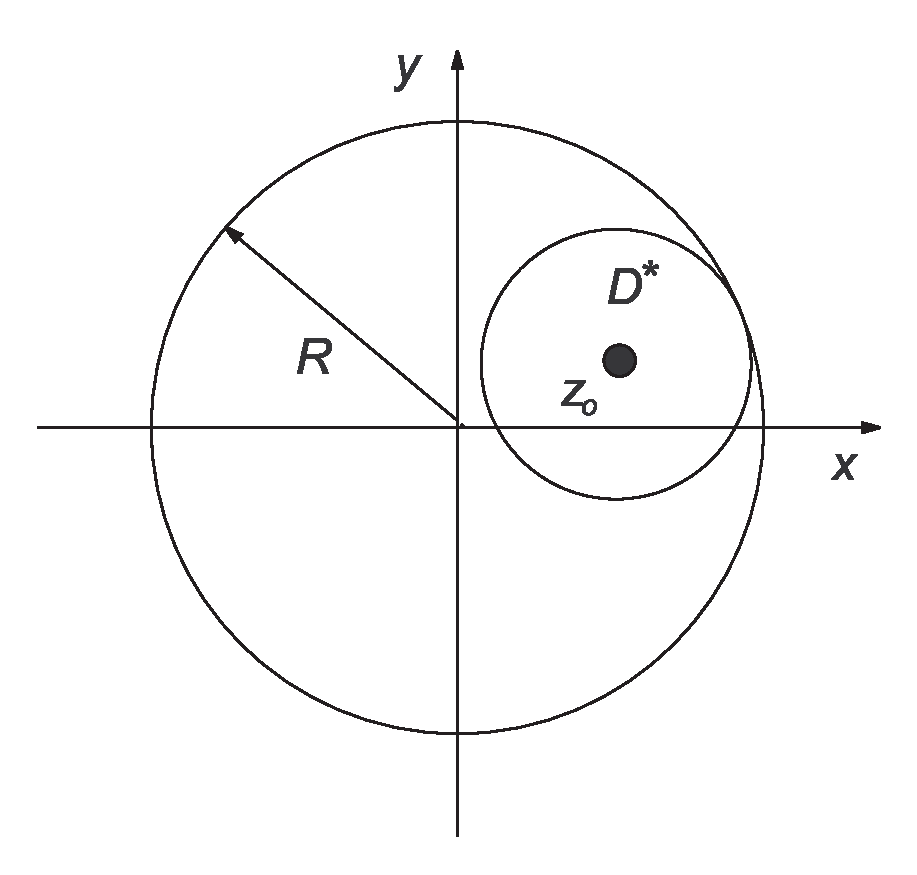
\includegraphics[width=0.4\textwidth]{fig-342.eps}
\caption{Centros diferentes}
\label{fig-342}
\end{figure}

Para estes valores de $z$ podemos, ordenar a s\'{e}rie no \'{u}ltimo
membro de \eqref{funre136:5} em fun\c{c}\~{a}o das pot\^{e}ncias de $Z =z -
z_o$, sem alterar sua soma. Desta maneira obtemos uma
representa\c{c}\~{a}o da forma
\begin{equation}\label{funre136:7}
  f(z)=\sum_{n\geq 0}a_n(z-z_o)^n
\end{equation}
v\'{a}lida (no m\'{\i}nimo) no disco
\begin{equation*}
  |z-z_o|<R-|z_o|.
\end{equation*}

Veremos mais tarde que, em geral, o raio de converg\^{e}ncia de
\eqref{funre136:7} ser\'{a} maior que $R- |z_o|$, de modo que
\eqref{funre136:7} fornece um \textit{prolongamento (continua\c{c}\~{a}o)}
da fun\c{c}\~{a}o $f$ em \eqref{funre136:1} para pontos fora do disco $|z|
< R$.

Este processo de prolongar uma fun\c{c}\~{a}o, dada inicialmente por uma
s\'{e}rie de pot\^{e}ncias v\'{a}lida em uma regi\~{a}o de converg\^{e}ncia $|z| < R$,
al\'{e}m desta regi\~{a}o \'{e} chamado prolongamento anal\'{\i}tico.

Pelo c\'{a}lculo direto segue-se que os coeficientes $a_n$ podem ser
representados em fun\c{c}\~{a}o dos coeficientes $a_n$, da representa\c{c}\~{a}o
original \eqref{funre136:1} sob a forma
\begin{equation}\label{funre136:8}
  a_n=\sum_{m\geq 0}{m+n\choose n }c_{m+n}b^m,\quad \text{ onde }\quad {m+n\choose n}=
  \frac{(m+n)!}{n!m!}
\end{equation}

A aplica\c{c}\~{a}o pr\'{a}tica de \eqref{funre136:8} ser\'{a} em geral dif\'{\i}cil.
Veremos ulteriormente, que no caso em que $f$ em
\eqref{funre136:1} \'{e} uma fun\c{c}\~{a}o conhecida, h\'{a} v\'{a}rios outros
m\'{e}todos de determinar os coeficientes da s\'{e}rie correspondente
\eqref{funre136:7}.

%%%%%%
\subsection{S\'{e}ries de Pot\^{e}ncias Representam Fun\c{c}\~{o}es Anal\'{\i}ticas}
%%%%%

Isto ser\'{a} o principal objetivo desta se\c{c}\~{a}o. Ap\'{o}s uma pequena
prepara\c{c}\~{a}o, deduziremos que cada fun\c{c}\~{a}o anal\'{\i}tica pode ser
representada por uma s\'{e}rie de pot\^{e}ncias, chamadas de S\'{e}ries de
Taylor.

\paragraph{Adi\c{c}\~{a}o ou Substra\c{c}\~{a}o de S\'{e}ries.}
A soma ou substra\c{c}\~{a}o de duas s\'{e}ries de pot\^{e}ncias com raios de
converg\^{e}ncia $R_1$ e $R_2$ respectivamente, fornecem uma s\'{e}rie de
pot\^{e}ncias com raio  menor o igual ao m\'{\i}nimo de $R_1$ e $R_2$.

\begin{prova} Consideremos as somas parciais $S_n(z)$ e $T_n(z)$. Somando termo
a termo e utilizando
\begin{equation*}
    \lim_{n\to\infty}\left\{S_n(z)\pm
    T_n(z)\right\}=\lim_{n\to\infty}S_n(z)\pm T_n(z),
\end{equation*}
com isso mostramos o que desejamos.\qed
\end{prova}

\paragraph{Multiplica\c{c}\~{a}o de S\'{e}ries de Pot\^{e}ncias.}
Consideramos duas s\'{e}ries de pot\^{e}ncias,
\begin{equation*}
    f(z)=\sum_{m\ge 0}a_mz^m\qquad g(z)=\sum_{m\ge 0}b_kz^k
\end{equation*}
e entendemos por multiplica\c{c}\~{a}o de s\'{e}ries de pot\^{e}ncias como a
multiplica\c{c}\~{a}o de cada termo da primeira s\'{e}rie com cada termo da
segunda s\'{e}rie, obtendo-se uma uma s\'{e}rie de pot\^{e}ncias em $z$
chamada de \textsc{Produto de Cauchy} das duas s\'{e}ries, e esta
representada por
\begin{equation*}
    f(z)g(z)=\sum_{n\ge 0}c_nz^n,\qquad c_n=\sum_{m+k=n}a_mb_k
\end{equation*}
onde
\begin{equation*}
c_n=\sum_{m+k=n}a_mb_k=a_ob_n+a_1b_{n-1}+\cdots+a_{n-1}b_1+a_nb_o
\end{equation*}

Esta s\'{e}rie converge absolutamente para cada $z$ que se encontra no
disco de converg\^{e}ncia de cada uma das s\'{e}ries dadas.

\paragraph{Deriva\c{c}\~{a}o e Integra\c{c}\~{a}o de S\'{e}ries de Pot\^{e}ncias.}
Examinamos a seguir a deriva\c{c}\~{a}o e a integra\c{c}\~{a}o termo a termo das
s\'{e}ries de pot\^{e}ncias. Derivando a s\'{e}rie $\dst{\sum_{n\geq 0}\,a_nz^n}$ obtemos a s\'{e}rie
\begin{equation}\label{funre136:9}
\sum_{n\geq 1}na_nz^{n-1}=a_1+2c_2z+3c_3z^2+\cdots
\end{equation}
que \'{e} chamada a s\'{e}rie derivada da s\'{e}rie dada.

\begin{theoc}{}{re136:3} 
A s\'{e}rie derivada de uma s\'{e}rie de pot\^{e}ncias possui o mesmo raio de converg\^{e}ncia 
que a s\'{e}rie original.
\end{theoc}

\prova Seja $na_n + a_n^*$. Ent\~{a}o $\sqrt[n]{|a_n^*|}
=\sqrt[n]{n}\sqrt[n]{|a_n|}$. Como $\sqrt[n]{n}$ vai para um
quando $n$ vai ao infinito segue-se que as sucess\~{o}es
$\sqrt[n]{|a_n^*|}$ e $\sqrt[n]{|a_n|}$, simultaneamente,
convergem para um mesmo limite ou ent\~{a}o divergem. Se elas
divergem, elas s\~{a}o ambas n\~{a}o-limitadas ou limitadas, e neste
\'{u}ltimo caso seus pontos de acumula\c{c}\~{a}o m\'{a}ximos s\~{a}o os mesmos. Da\'{\i} e
do Teorema~\ref{thm:re136:2} da \'{u}ltima se\c{c}\~{a}o decorre a validade do
presente teorema. \hfill $\square$

\begin{theoc}{}{re136:4}
A s\'{e}rie de potências,
\begin{equation*}
\sum_{n\geq 0}\frac{a_n}{n+1}z^{n+1}=a_{0}z+\frac{a_1}{2}z^2+\frac{a_2}{3}z^3+\cdots
\end{equation*}
obtida integrando a s\'{e}rie $a_{0} + a_1z + a_2z^2+\cdots$ termo a
termo possui o mesmo raio de converg\^{e}ncia que a s\'{e}rie original.
\end{theoc}

\begin{prova}
A demonstra\c{c}\~{a}o \'{e} semelhante \`{a} do Teorema~\ref{thm:re136:3}.\qed
\end{prova}

\begin{exer} Considere s\'{e}rie de pot\^{e}ncias
\begin{equation*}
  \sum_{n\geq 1}(n+1)\,z^{n}
\end{equation*}
encontre seu raio de converg\^{e}ncia.
\end{exer}

\begin{solo}
 Para encontrar o raio de converg\^{e}ncia, integramos termo a termo
 e obtemos a s\'{e}rie geom\'{e}trica $\sum_{}\,z^{n+1}$ com raio $R = 1$. \hfill \(\lozenge\)
\end{solo}

As s\'{e}ries de pot\^{e}ncias representam fun\c{c}\~{o}es anal\'{\i}ticas. Mais precisamente.

\begin{theoc}{}{re136:5} 
Uma s\'{e}rie de pot\^{e}ncias com raio de converg\^{e}ncia n\~{a}o-nulo
$R$, representa uma fun\c{c}\~{a}o anal\'{\i}tica em todos os pontos no
interior de seu disco de converg\^{e}ncia. As derivadas desta fun\c{c}\~{a}o
s\~{a}o obtidas, derivando a s\'{e}rie original termo a termo; todas as
s\'{e}ries assim obtidas possuem o mesmo raio de converg\^{e}ncia que a
s\'{e}rie original.
\end{theoc}

\begin{prova} Consideramos a representa\c{c}\~{a}o
\begin{equation*}
f(z)=\sum_{n\geq 0}a_nz^{n},
\end{equation*}
supondo que o raio de converg\^{e}ncia $R$ n\~{a}o \'{e} nulo. Ent\~{a}o podemos
representar $f$ sob a forma \eqref{funre136:7}, e do
Teorema~\ref{thm:re136:1} segue-se que $f$ \'{e} cont\'{\i}nua com centro em
$z_{0}$. Como $z_o$ \'{e} um ponto qualquer no disco $|z|< R$, a fun\c{c}\~{a}o
$f(z)$ \'{e} cont\'{\i}nua em todo o disco. De \eqref{funre136:7} obtemos
$f(z_{0})=a_{0}$ e, portanto,
\begin{equation*}
  \frac{f(z)- f(z_{0})}{z-z_{0}}=a_1 + a_2(z - z_{0}) + a_3(z - z_{0})^2 +
  \cdots
\end{equation*}

De acordo com o Teorema~\ref{thm:re136:1}, a fun\c{c}\~{a}o representada pela
s\'{e}rie de pot\^{e}ncias no segundo membro \'{e} cont\'{\i}nua em $z_o$. Assim,
de acordo com \eqref{funre136:8},
\begin{align}
  f'(z_{0})=\lim_{z\to z_{0}}\frac{f(z)-f(z_{0})}{z-z_{0}} =a_1&=\sum_{m\geq 0}(m+1)a_{m+1}z_{0}^{m}
  \nonumber\\[2ex]
   &=\sum_{k\geq 1}ka_kz_o^{k-1}\label{funre136:10}
\end{align}

Isto mostra que a primeira derivada de $f$ existe em um ponto $z = z_{0}$ do disco $|z|<R$, e pode ser obtida derivando 
a s\'{e}rie original termo a termo; de fato, a s\'{e}rie no \'{u}ltimo membro possui
raio de converg\^{e}ncia $R$, como foi demonstrado no
Teorema~\ref{thm:re136:3}.  Assim $f$ \'{e} anal\'{\i}tica no disco $|z|< R$ e
a demonstra\c{c}\~{a}o fica completa. \qed
\end{prova}

\begin{exer} Considere s\'{e}rie de pot\^{e}ncias
\begin{equation*}
\sum_{n\geq 2}\binom{n}{2}z^{n}=z^2+3z^3+6z^4+10z^5+\cdots
\end{equation*}
encontre seu raio de converg\^{e}ncia.
\end{exer}

\solo
 Para encontrar o raio de converg\^{e}ncia, derivamos duas vezes termo a termo
 a s\'{e}rie geom\'{e}trica $\sum_{}z^{n+1}$ com raio $R = 1$ e multiplicamos o resultado pelo
fator $z^2/2$ para obter a s\'{e}rie dada, logo o raio procurado \'{e}
$R=1$.\hfill \(\lozenge\)

Como a derivada da  fun\c{c}\~{a}o $f$ \'{e}
\begin{equation*}
  f'(z)= \sum_{n\,=\, 1}^{\infty}\, na_nz^{n-1}
\end{equation*}
e \'{e} representada por uma s\'{e}rie de pot\^{e}ncias, podemos aplicar o
Teorema~\ref{thm:re136:5} a $f'$, concluir que $f''$ existe no disco
$|z|<R$, e
\begin{equation*}
  f''(z)=\sum_{n\geq 2}n(n-1)\,a_{n}z^{n-2}
\end{equation*}

Mais geralmente, a derivada de ordem $m$, $f^{(m)}$, de $f$ existe
no disco e
\begin{equation}\label{funre136:11}
f^{(m)}(z)=\sum_{n\geq m} n(n - 1)\cdots(n - m + 1)a_nz^{n-m}.
\end{equation}

Isto significa que $f$ possui derivadas de todas as ordens no
disco. Veremos mais tarde  que toda fun\c{c}\~{a}o anal\'{\i}tica possui
derivadas de todas as ordens e, al\'{e}m disso, pode ser representada
por uma s\'{e}rie de pot\^{e}ncias.

%%%%%%%%%
\section*{Exercícios Propostos} 
%%%%%%%%%
Resolver os seguintes exerc\'{\i}cios sobre s\'{e}ries de fun\c{c}\~{o}es,
\begin{enumerate}[label=\rm{(\arabic*)},ref=\rm{(\arabic*)}]
\item Utilizando o Teorema~\ref{thm:re136:2}, provar que se $f(z)$ em \eqref{funre136:1} for uma
fun\c{c}\~{a}o \'{\i}mpar, ent\~{a}o $a_n =0$ para $n=0,2,4,\ldots$. Dar exemplos.
\item Mostrar que se $f(z)$ em \eqref{funre136:1} for par, ent\~{a}o $a_n = 0$ para $n = 1,
3, 5,\ldots$.
\item Mostrar que $\dst{f(z)=\sum_{n\geq 0}\frac{z^n}{n!}}$ n\~{a}o \'{e} nem par nem \'{\i}mpar.
\item  Utilizando a s\'{e}rie geom\'{e}trica, verificar as afirma\c{c}\~{o}es dos Teoremas~\ref{thm:re136:3}
e \ref{thm:re136:4}.
\item Verificar os Teoremas~\ref{thm:re136:3} e \ref{thm:re136:4} para a
s\'{e}rie$\dst{f(z)=\sum_{n\geq 0}\frac{z^n}{n!}}$.
\item Empregando a s\'{e}rie geom\'{e}trica e os Teoremas~\ref{thm:re136:3} e \ref{thm:re136:4}, determinar os
raios de converg\^{e}ncia das seguintes s\'{e}ries
\begin{tasks}[label=\rm{(\alph*)},item-indent=4em,label-width=4ex,ref=\rm{(\alph*)}](2)
\task  \(\dst \sum_{n\geq 0}\,n(z-j)^{n}\quad   R: \)
\task  \(\dst \sum_{n\geq k}{n\choose k}\,z^{n}\quad  R:\)
\task  \(\dst \sum_{n\geq k}{n\choose k}\left(\dfrac{z}{3}\right)^{n}\quad  R: \)
\task  \(\dst \sum_{n\geq 1}\frac{(-1)^n}{n}(z+1)^{n}\quad  R:\)
\task  \(\dst \sum_{n\geq 1}\frac{z^n}{2^n n(n-1)}\quad  R: \)
\task  \(\dst \sum_{n\geq 1}\frac{(z-2i)^n}{3^n n}\quad  R:\)
\end{tasks}
\item Utilizando o Teorema~\ref{thm:re136:5}, demonstrar as seguintes proposi\c{c}\~{o}es,
\begin{tasks}[label=\rm{(\alph*)},item-indent=4em,label-width=4ex,ref=\rm{(\alph*)}](1)
\task \(\dst{f(z)=\sum_{n\geq 0}\frac{z^n}{n!}}\quad \textrm{ satisfaz a }\quad  f'(z)-f(z)=0\)
\task \(\dst{f(z)=\sum_{n\geq 0}\frac{(-1)^n}{(2n)!}z^{2n}} \quad \textrm{satisfaz a} \quad  f''(z)+f(z)=0\)
\task \(\dst{f(z)=\sum_{n\geq 0}\frac{(-1)^n}{(2n+1)!}z^{2n+1}}\quad  \textrm{ satisfaz a } \quad  f''(z)+f(z)=0.\)
\end{tasks}
\end{enumerate}

%%%%%
\section{S\'{e}rie de Taylor}
%%%%
Na \'{u}ltima se\c{c}\~{a}o vimos que s\'{e}ries de pot\^{e}ncias com raio de converg\^{e}ncia n\~{a}o-nulo representam fun\c{c}\~{o}es anal\'{\i}ticas. Veremos agora que toda fun\c{c}\~{a}o anal\'{\i}tica pode ser representada por uma s\'{e}rie de pot\^{e}ncias. Estas representa\c{c}\~{o}es s\~{a}o chamadas s\'{e}ries de Taylor e s\~{a}o semelhantes \`{a}s s\'{e}ries de Taylor familiares das fun\c{c}\~{o}es reais. Na verdade, substituindo a vari\'{a}vel real nas s\'{e}ries reais por uma vari\'{a}vel complexa podemos prolongar fun\c{c}\~{o}es reais de maneira anal\'{\i}tica dentro do dom\'{\i}nio complexo.


O desenvolvimento familiar em s\'{e}rie de Taylor constitui uma ferramenta eficaz no c\'{a}lculo real e em suas aplica\c{c}\~{o}es. Veremos que na an\'{a}lise complexa o desenvolvimento de Taylor, que \'{e} uma generaliza\c{c}\~{a}o do desenvolvimento acima mencionado, \'{e} ainda mais importante.

Consideramos uma fun\c{c}\~{a}o $f$, que \'{e} anal\'{\i}tica em uma vizinhan\c{c}a de um ponto $z$. Seja $\mathcal{C}$  uma circunfer\^{e}ncia  nesta vizinhan\c{c}a e possui o centro $z$. Podemos ent\~{a}o aplicar a f\'{o}rmula integral de Cauchy,
\begin{equation}\label{tay141:1}
\oint_{\mathcal{C}}\frac{f(w)}{w-z}dw=(2\pi j)f(z)
\end{equation}
onde $z$ \'{e} um ponto fixo arbitr\'{a}rio no interior de $\mathcal{C}$ e
$w$ \'{e} a vari\'{a}vel complexa de integra\c{c}\~{a}o. Temos,
\begin{equation}\label{tay141:2}
 \frac{1}{w - z}=\frac{1}{w - a - (z- a)}= \frac{1}{(w - a)( 1 - \frac{z - a}{w -
 a})}
\end{equation}

Notamos que como $w$ est\'{a} sobre $ \mathcal{C}$ enquanto $z$ est\'{a}
no interior de $ \mathcal{C}$,
\begin{equation}\label{tay141:3}
 \left|\frac{z - a}{w-a}\right| < 1
\end{equation}

Da progress\~{a}o geom\'{e}trica
\begin{equation*}
  1 + q + q^2 +\cdots+ q^n=\frac{1-q^{n+1}}{1- q}=\frac{1}{1- q}-\frac{q^{n+1}}{1- q},\qquad q\neq 1
\end{equation*}
obtemos a rela\c{c}\~{a}o
\begin{equation*}
\frac{1}{1-q}=1 +q +\cdots + q^n + \frac{q^{n+1}} {1- q}
\end{equation*}

Fazendo $q =(z - a)/(w- a)$ segue-se que

\begin{align*}
\frac{1}{1-[(z-a)/(w-a)]} = 1 &+ \frac{z - a}{w-a} +
\left(\frac{z- a}{w-a}\right)^2 +\cdots\\[2ex]
&\cdots+ \left(\frac{z- a}{w - a}\right)^n+\frac{[(z - a)/(w -
a)]^{n+1}}{(w - z)/(w - a)}
\end{align*}

Substitu\'{\i}mos esta express\~{a}o em \eqref{tay141:2}, e ent\~{a}o
\eqref{tay141:2} em \eqref{tay141:1}. Como $z$ e $a$ s\~{a}o
constantes, podemos retirar do sinal de integral as pot\^{e}ncias de
$(z - a)$, e \eqref{tay141:1} passa a apresentar a forma
\begin{align}\label{tay141:4}
  f(z)&=\frac{1}{2\pi j}\oint_{\mathcal{C}}\frac{f(w)}{w-a}dw+
  \frac{z-a}{2\pi j}\oint_{\mathcal{C}}\frac{f(w)}{(w-a)^2}dw+\cdots \nonumber\\[2ex]
   &\quad\cdots + \frac{(z-a)^n}{2\pi j}\oint_{\mathcal{C}}\frac{f(w)}{(w-a)^{n+1}}dw+R_n(z)
\end{align}
onde o \'{u}ltimo termo \'{e} dado pela f\'{o}rmula
\begin{equation}\label{tay141:5}
R_n(z)=  \frac{(z- a)^{n+1}}{ 2\pi
j}\oint_{\mathcal{C}}\frac{f(w)}{(w-a)^{n+1}(w-z)}dw.
\end{equation}

Empregando a derivada geral,
\begin{equation*}
  f^{(n)}(a)=\frac{n!}{2\pi
  ij}\oint_{\mathcal{C}}\frac{f(w)}{(w-a)^{n+1}}dw,\qquad
  n=1,2,3,\ldots
\end{equation*}
podemos escrever \'{e}ste desenvolvimento sob a forma
\begin{align}\label{tay141:6}
f(z)= f(a)&+ \frac{(z-a)}{1!} f'(a)+\frac{(z - a)^2}{2!}f''(a)+\cdots\nonumber\\[2ex]
   &\cdots+ \frac{(z - a)^n}{n!} f^{(n)}(a) + R_n(z).
\end{align}

Esta representa\c{c}\~{a}o constitui a \textsc{F\'{o}rmula de Taylor}.
$R_n(z)$ \'{e} chamado o resto.

Como a fun\c{c}\~{a}o anal\'{\i}tica $f$ possui derivadas de todas as ordens,
podemos tomar $n$ em \eqref{tay141:6} arbitrariamente grande.

Fazendo $n$ se aproximar do infinito, obtemos de \eqref{tay141:6}
a s\'{e}rie de pot\^{e}ncias
\begin{equation}\label{tay141:7}
f(z)=\sum_{m\geq 0}\frac{f^{(m)}(a)}{m!}(z - a)^m.
\end{equation}

Esta s\'{e}rie \'{e} a chamada \textsc{S\'{e}rie de Taylor} de $f$ com centro
em $a$. O caso particular em que $a = 0$ constitui a chamada
\textsc{s\'{e}rie de Maclaurin} de $f$.

Evidentemente, a s\'{e}rie \eqref{tay141:7} converge e representa $f$
se, e somente, se,
\begin{equation}\label{tay141:8}
\lim_{n\to\infty} R_n(z) = 0.
\end{equation}

Para demonstrar \eqref{tay141:8}, consideramos \eqref{tay141:5}.
Como $w$ se encontra sobre $ \mathcal{C}$ enquanto $z$ est\'{a} no
interior de $ \mathcal{C}$, temos $|w - z|>0$. Como $f$ \'{e}
anal\'{\i}tica no interior de $ \mathcal{C}$ e sobre $\mathcal{C}$,
segue-se que o valor absoluto de $f(w)/(w-z)$ \'{e} limitado, digamos
\begin{equation*}
\left|\frac{f(w)}{w - z}\right|<T
\end{equation*}
para todo $w$ sobre $\mathcal{C}$. Seja $r$ o raio de $
\mathcal{C}$. Ent\~{a}o, $ \mathcal{C}$ possui o comprimento $2\pi r$,
e $|w - a | = r$ para todo $w$ sobre $\mathcal{C}$. Assim,
aplicando a f\'{o}rmula fundamental
\begin{equation*}
\left|\oint_{\mathcal{C}} f(z)dz \right|\leq M\cdot L
\end{equation*}
onde $L$ \'{e} o comprimento da tra\c{c}o da curva $\mathcal{C}$ e $M$ \'{e}
uma constante real tal que $|f(z)|\le M$ em qualquer ponto de
$\mathcal{C}$, a \eqref{tay141:5}, obtemos
\begin{align*}
|R_n| &= \frac{|z -a|^{n+1}}{2\pi}\left|\oint_{\mathcal{C}}
\frac{f(w)}{(w -a)^{n+1}(w-z)}dw\right|\\[2ex]
  &<\frac{|z -a|^{n+1}}{2\pi}T\frac{1}{r^{n+1}}2\pi r=T\,r\left|
  \frac{z-a}{r}\right|^{n+1}
\end{align*}

Observamos que $|z-a|<r$ para $z$ dentro ds circunf\^{e}rencia
$\mathcal{C}$, assim $|z-a|/r<1$. Fazendo $n$ se aproximar do
infinito,  a express\~{a}o \`{a} direita se aproxima de zero. Isto
demonstra \eqref{tay141:8} para todo $z$ no interior de $
\mathcal{C}$. Como, pelo Teorema~\ref{thm:re136:2}, a representa\c{c}\~{a}o de
$f$ sob a forma \eqref{tay141:7} \'{e} \'{u}nica, no sentido de que
\eqref{tay141:7} \'{e} a \'{u}nica s\'{e}rie de pot\^{e}ncias com centro em $a$,
que representa a fun\c{c}\~{a}o dada $f$, podemos resumir o resultado como
segue.

\begin{theoc}{Teorema de Taylor}{} Seja $f$ anal\'{\i}tica em um dom\'{\i}nio $\Om$ e seja
$z=a$ um ponto qualquer em $\Om$. Existe, ent\~{a}o, unicamente uma
s\'{e}rie de pot\^{e}ncias com centro em $a$ que representa $f$; esta
s\'{e}rie \'{e} da forma
\begin{equation}\label{tay141:9}
f(z)=\sum_{n\geq 0}b_n(z - a)^n,\quad \text{onde} \quad
b_n=\frac{1}{n!}f^{(n)}(a),\quad n=0,1,\ldots
\end{equation}

Esta representa\c{c}\~{a}o \'{e} v\'{a}lida no disco aberto m\'{a}ximo com centro $a$,
contido em $\Om$. O resto $R_n(z)$ de \eqref{tay141:9} pode ser
representado sob a forma \eqref{tay141:5}. Os coeficientes
satisfazem, \`{a} desigualdade
\begin{equation}\label{tay141:10}
|b_n|\le \frac{M}{r^n}
\end{equation}
onde $M$ \'{e} o m\'{a}ximo de $|f(z)|$  sobre o circunfer\^{e}ncia $|z - a|=
r$.
\end{theoc}

A rela\c{c}\~{a}o \eqref{tay141:10} decorre da desigualdade
\begin{equation*}
  |f^{(n)}(z)|\le \frac{n!M}{r^n}
\end{equation*}
chamada de Cauchy.

Em termos pr\'{a}ticos, \eqref{tay141:8} significa que para todo $z$
para o qual \eqref{tay141:9} converge, a soma parcial de ordem $n$
de \eqref{tay141:9} se aproxima de $f$ com qualquer precis\~{a}o
estabelecida; temos unicamente que escolher $n$ suficientemente
grande.

De acordo com o Teorema de Taylor vemos que o raio de converg\^{e}ncia
de \eqref{tay141:9} \'{e} no m\'{\i}nimo igual \`{a} menor dist\^{a}ncia de $a$ ao
contorno de $\Om$. Ele pode ser maior, mas ent\~{a}o a s\'{e}rie pode n\~{a}o
mais representar $f$ em todos os pontos de $\Om$ que se encontram
no interior do disco de converg\^{e}ncia.

\paragraph{Compara\c{c}\~{a}o com Fun\c{c}\~{o}es de Vari\'{a}vel Real.} Uma
propriedade surpreendente das fun\c{c}\~{o}es anal\'{\i}ticas complexas,
consiste em que elas possuem derivadas, de todas as ordens; outra,
que acabamos de expor, consiste em que elas podem ser sempre
representadas por s\'{e}ries de pot\^{e}ncias da forma \eqref{tay141:9}.
Esta propriedade em geral n\~{a}o \'{e} verdadeira para fun\c{c}\~{o}es reais; h\'{a}
fun\c{c}\~{o}es reais que possuem derivadas de todas as ordens mas n\~{a}o
podem ser representadas por s\'{e}ries de pot\^{e}ncias. Por exemplo a
seguinte fun\c{c}\~{a}o
\begin{equation*}
    f(x)=\left\{%
\begin{array}{ll}
    e^{-1/x^2} & \hbox{ se }\quad x\neq 0 \\[2ex]
    0 & \hbox{ se }\quad x=0 
\end{array}%
\right.
\end{equation*}
esta fun\c{c}\~{a}o n\~{a}o pode ser representada por uma s\'{e}rie de Taylor ao
redor de $z=0$ pois todas a sus derivadas s\~{a}o nulas no ponto
$z=0$.

A rela\c{c}\~{a}o entre o presente estudo e o assunto da se\c{c}\~{a}o anterior
sobre s\'{e}ries de pot\^{e}ncias, pode ser estabelecida pelo seguinte
teorema:

\begin{theoc}{}{ta141:2} 
Toda s\'{e}rie de pot\^{e}ncia com um raio de converg\^{e}ncia n\~{a}o
nulo \'{e} a s\'{e}rie de Taylor da fun\c{c}\~{a}o representada por esta s\'{e}rie.
\end{theoc}

\begin{prova}
Seja a s\'{e}rie de pot\^{e}ncias
\begin{equation*}
  \sum_{n\geq 0}b_n(z - a)^n
\end{equation*}
com um raio de converg\^{e}ncia n\~{a}o nulo $R$. Ent\~{a}o ela representa uma
certa fun\c{c}\~{a}o anal\'{\i}tica $f$ no disco $| z - a | < R$, isto \'{e},
\begin{equation*}
f(z) = b_o + b_1(z -a) + b_2(z - a)^2 +\cdots
\end{equation*}

Do Teorema~\ref{thm:re136:5} segue-se que
\begin{equation*}
  f'(z) = b_1 + 2b_2(z - a) +\cdots
\end{equation*}
e mais geralmente
\begin{equation*}
f^{(n)}(z) = n!\, b_n + (n + 1)\cdot n \cdots 3\cdot2\cdot1\,
b_{n+1}(z - a) +\cdots;
\end{equation*}
todas estas s\'{e}ries convergem no disco $| z - a | < R$. Fazendo $z
= a$ obtemos as seguintes representa\c{c}\~{o}es para os coeficientes da
s\'{e}rie de pot\^{e}ncias:
\begin{equation*}
f(a) = b_o,\quad f'(a) = b_1,\quad\ldots,\quad f^{(n)}(a) = n!
\,b_n,\ldots
\end{equation*}

Estas f\'{o}rmulas s\~{a}o id\^{e}nticas \`{a}s do teorema de Taylor, ent\~{a}o a
demonstra\c{c}\~{a}o est\'{a} completa. \qed
\end{prova}

A f\'{o}rmula da intergral de Cauchy ajuda para expressar os
coeficientes da S\'{e}rie de Taylor
\begin{equation*}
    b_n=\frac{f^{(n)}(a)}{n!}=\frac{1}{2\pi
    j}\oint_{\mathcal{C}}\frac{f(z)}{(z-a)^{n+1}}dz
\end{equation*}
onde se integra no sentido anti-hor\'{a}rio sobre a curva simples e
fechada $\mathcal{C}$, que contem em seu interior o ponto $z=a$.

O ponto em que uma fun\c{c}\~{a}o $f$ deixa de ser anal\'{\i}tica \'{e} chamado um
\textbf{ponto singular} de $f$; podemos tamb\'{e}m dizer que $f$
possui uma singularidade em tal ponto. Mais precisamente: um ponto
$z =z_o$ \'{e} chamado um \textbf{ponto singular} de $f$, se $f$ n\~{a}o
for deriv\'{a}vel em $z_o$ mas, qualquer vizinhan\c{c}a de $z_o$ cont\'{e}m
pontos em que $f$ \'{e} deriv\'{a}vel.

Empregando esse conceito, podemos dizer que existe no m\'{\i}nimo um
ponto singular de $f$ no disco de converg\^{e}ncia isto \'{e}, o raio de
converg\^{e}ncia de \eqref{tay141:9} \'{e}, em geral, igual \`{a} dist\^{a}ncia de
$a$ ao ponto singular de $f$ mais pr\'{o}ximo, mas pode ser maior; por
exemplo, $\ln z$ \'{e} singular ao longo do semi-eixo real negativo, e
a dist\^{a}ncia de $a = - 1 + j$ \`{a}quele eixo \'{e} $1$; entretanto a s\'{e}rie
de Taylor de $\ln z$ com $a = - 1 + j$ tem  raio de converg\^{e}ncia
$\sqrt{2}$.

\subsection{S\'{e}ries de Taylor das Fun\c{c}\~{o}es Elementares}

\begin{exer}[S\'{e}rie Geom\'{e}trica] Seja $f$ uma fun\c{c}\~{a}o complexa de vari\'{a}vel complexa  tal que
$f(z) = 1/(1-z)$. Encontre o seu desenvolvimento de Maclaurin.
\end{exer}

\solo Temos ent\~{a}o $f^{(n)}(z) =n! /(1 - z)^{n+1}$,
$f^{(n)}(z)=n!/(1-z)^{n+1}$. Assim o desenvolvimento de Maclaurin
de $1/(1 - z)$ \'{e} a s\'{e}rie geom\'{e}trica
\begin{equation}\label{elem142:1}
\frac{1}{1-z}=\sum_{n\geq 0}z^n=1 + z + z^2 +\cdots \qquad  |z|
<1,
\end{equation}
logo $f$ \'{e} singular em $z=1$;  este ponto se situa sobre o c\'{\i}rculo
de converg\^{e}ncia. \hfill \(\lozenge\)


\begin{exer}[Fun\c{c}\~{a}o Exponencial]
Considere a fun\c{c}\~{a}o exponencial $e^z$. Analizar suas propriedades.
\end{exer}

\solo  A fun\c{c}\~{a}o exponencial $e^z$
 \'{e} anal\'{\i}tica para qualquer $z$ e que $(e^z)'=e^z$.
Assim, de acordo com \eqref{tay141:9}, com $a = 0$, obtemos a
s\'{e}rie de Maclaurin
\begin{equation}\label{elem142:2}
 e^z =\sum_{n\geq 0}\frac{z^n}{n!}=1+z+z^2+z^3+\cdots
\end{equation}

Esta s\'{e}rie \'{e} tamb\'{e}m obtida quando substitu\'{\i}mos $x$ na s\'{e}rie de
Maclaurin de $e^x$, por $z$. Exprimimos isso afirmando que
prolongamos analiticamente a fun\c{c}\~{a}o exponencial real no dom\'{\i}nio
complexo. \hfill \(\lozenge\)

\bigskip
Provemos a f\'{o}rmula de multiplica\c{c}\~{a}o
\begin{equation}\label{elem142:3}
e^{z_1}e^{z_2}=e^{z_1+z_2}
\end{equation}
empregando \eqref{elem142:2}. Temos
\begin{equation*}
e^{z_1}e^{z_2}=\sum_{k\geq 0}\frac{z_1^k}{k!}\;\sum_{m\geq
0}\frac{z_2^m}{m!}
\end{equation*}

Como ambas as s\'{e}ries convergem absolutamente, podemos
multiplic\'{a}-las termo a termo; a soma dos produtos para os quais $k
+ m= n$ \'{e}
\begin{align*}
\frac{z_1^n}{n!}+\frac{z_1^{n-1}}{(n-1)!}\frac{z_2}{1!}+\cdots+
\frac{z_1}{1!}\frac{z_2^{n-1}}{(n-1)!}+\frac{z_2^n}{n!}&=\\[2ex]
\frac{1}{n!}\left[z_1^n+{n\choose 1}z_1^{n-1}z_2+{n\choose
2}z_1^{n-2}z_2^2+\cdots+z_2^n \right]&=\frac{(z_1+z_2)^n}{n!}
\end{align*}

Ent\~{a}o o produto das duas s\'{e}ries pode ser escrito
\begin{equation*}
\sum_{n\geq 0}\frac{(z_1+z_2)^n}{n!}=e^{z_1+z_2}
\end{equation*}
ficando \eqref{elem142:3} demonstrada.\qed

Al\'{e}m disso, fazendo $z =jy$ em \eqref{elem142:2} e aplicando a
propriedade de adi\c{c}\~{a}o das s\'{e}ries convergentes, obtemos
\begin{equation*}
e^{jy}=\sum_{n\geq 0}\frac{(jy)^n}{n!}=\sum_{k\geq 0}(-1)^k
\frac{y^{2k}}{(2k)!}+j\sum_{k\geq 0}(-1)^k
\frac{y^{2k+1}}{(2k+1)!}
\end{equation*}

Como as s\'{e}ries do segundo membro s\~{a}o os desenvolvimentos de
Maclaurin familiares das fun\c{c}\~{o}es reais $\cos y$ e $\sen y$, este
resultado representa a f\'{o}rmula de Euler
\begin{equation}\label{elem142:4}
e^{jy} = \cos y + j \sen y;
\end{equation}

Multiplicando por $e^x$ e empregando \eqref{elem142:3}, obtemos a
f\'{o}rmula,
\begin{equation*}
e^z=e^x(\cos y +j\sen y)
\end{equation*}
que foi empregada para definir $e^z$. A presente exposi\c{c}\~{a}o mostra
que \'{e} poss\'{\i}vel tamb\'{e}m empregar \eqref{elem142:2} para definir
$e^z$ e deduzir de \eqref{elem142:2} todas as f\'{o}rmulas obtidas nas
se\c{c}\~{o}es anteriores. \qed

\begin{exer}[Fun\c{c}\~{o}es Trigonom\'{e}tricas e Hiperb\'{o}licas]
Escrever as f\'{o}rmulas das fun\c{c}\~{o}es trigom\'{e}tricas e hiperb\'{o}licas em
s\'{e}ries de pot\^{e}ncias.
\end{exer}

\solo  Substituindo o desenvolvimento da exponencial \eqref{elem142:2} nas defini\c{c}\~{o}es de $\sen
z$ e $\cos z$ , obtemos
\begin{align}\label{elem142:5}
  \cos(z) & = \sum_{n\geq 0}(-1)^n\frac{z^{2n}}{(2n)!}=1-\frac{z^2}{2!}+\frac{z^4}{4!}+\cdots\\[2ex]
  \sen(z) &= \sum_{n\geq 0}(-1)^n\frac{z^{2n+1}}{(2n+1)!}=z-\frac{z^3}{3!}+\frac{z^5}{5!}+\cdots
\end{align}

Quando $z = x$ estas s\'{e}ries se transformam nas s\'{e}ries familiares
das fun\c{c}\~{o}es reais $\cos x$ e $\sen x$. Semelhantemente,
substituindo \eqref{elem142:2} em nas defini\c{c}\~{o}es de $\senh z$ e
$\cosh z$ obtemos
\begin{align}\label{elem142:6}
  \cosh(z) &=\sum_{n\geq 0}\frac{z^{2n}}{(2n)!}=1+\frac{z^2}{2!}+\frac{z^4}{4!}+\cdots \\[2ex]
  \senh(z) &=\sum_{n\geq
  0}\frac{z^{2n+1}}{(2n+1)!}=z+\frac{z^3}{3!}+\frac{z^5}{5!}+\cdots
\end{align}

Obtendo assim o que desejavamos. \hfill \(\lozenge\)

\begin{exer}[Logaritmo]
Escrever  a fun\c{c}\~{a}o complexa,  $\dst{\ln\left(\frac{1 +
z}{1-z}\right)}$ em s\'{e}ries de pot\^{e}ncias, utilizando propriedades.
\end{exer}

\solo Pelo Teorema de Taylor, equa\c{c}\~{a}o \eqref{tay141:9} decorre que
\begin{equation}\label{elem142:7}
\ln(1 + z) = z - \frac{z^2}{2} + \frac{z^3 }{3}- \cdots,\qquad
|z|<1.
\end{equation}

Substituindo $z$ por $-z$ e multiplicando ambos os lados por $-
1$, obtemos
\begin{equation}\label{elem142:8}
-\ln(1-z) = \ln \frac{1}{1-z} = z + \frac{z^2}{2} + \frac{z^3}{3}
+\cdots \qquad | z |<1.
\end{equation}

Adicionando ambas as s\'{e}ries obtemos
\begin{equation}\label{elem142:9}
\ln \left(\frac{1 + z}{1-z}\right) = 2
\left[z+\frac{z^3}{3}+\frac{z^5}{5}+\cdots \right]\qquad |z|<1,
\end{equation}
obtemos o que desejamos.\hfill \(\lozenge\)

%%%%%%%
\section*{Exerc\'{\i}cios Propostos} 
%%%%%%%
Resolva os seguintes exerc\'{\i}cios sobre s\'{e}ries de po\^{e}ncias complexas.
\begin{enumerate}[label=\rm{(\arabic*)},ref=\rm{(\arabic*)}]
\item Deduzir as s\'{e}ries de Taylor, em torno do ponto $z = a$, das
fun\c{c}\~{o}es seguintes, e determinar o raio de converg\^{e}ncia.
\begin{tasks}[label=\rm{(\alph*)},item-indent=3em,label-width=4ex,ref=\rm{(\alph*)}](2)
\task \(\cos(2z), \quad   a = 0 \)
\task \(\sen(z^2),\quad a = 0\)
\task \(e^{-z},\quad  a = 0 \)
\task \(e^z,\quad a = 1\)
\task \(e^z,\quad a= \pi i\)
\task \(\sen(z),\quad  a= \pi/2\)
\task \(\cos(z),\quad  a = - \pi/4\)
\task  \(1/(1-z),\quad   a =-1\)
\task \(1/z,\quad   a = 1\)
\task \(1/(1 - z),\quad   a = i\)
\task \(\cos^2(z),\quad   a = 0\)
\task \(\sen^2(z),\quad   a =0\)
\end{tasks}
\item Determinar os tr\^{e}s primeiros termos das s\'{e}ries de Maclaurin
das fun\c{c}\~{o}es seguintes.
\begin{tasks}[label=\rm{(\alph*)},item-indent=3em,label-width=4ex,ref=\rm{(\alph*)}](2)
\task \(\tan(z)\)
\task \(\tan(2z)\)
\task \(e^z \sen(z)\)
\task \(z \cot(z)\)
\end{tasks}
\item Determinar as s\'{e}ries de Maclaurin integrando termo a termo as
dos integrandos.
\begin{tasks}[label=\rm{(\alph*)},item-indent=3em,label-width=4ex,ref=\rm{(\alph*)}](2)
\task  \(\dst{\int_0^z e^t\, dt}\)
\task \(\dst{\int_0^z \cos(t)\, dt}\)
\task \(\dst{\int_0^z \sen(t)\, dt}\)
\task \(\dst{\int_0^z \frac{e^t-1}{t}\, dt}\)
\task \(\dst{\int_0^z e^{t^2}\,dt}\)
\task \(\dst{\int_0^z \frac{\sen t}{t}\, dt}\)
\task \(\dst{\int_0^z \cos(t^2)\, dt}\)
\task \(\dst{\int_0^z \sen(t^2)\, dt}\)
\end{tasks}
\end{enumerate}

%%%%%
\section{M\'{e}todos para Obten\c{c}\~{a}o de S\'{e}ries de Pot\^{e}ncias}
%%%%
Na maioria dos casos pr\'{a}ticos, a determina\c{c}\~{a}o dos coeficientes de
uma s\'{e}rie de Taylor por meio da f\'{o}rmula do teorema de Taylor \'{e}
complicada, ou consome muito tempo. Existe um certo n\'{u}mero de
processos pr\'{a}ticos mais simples para atingir tal fim, que podem
ser ilustrados pelos seguintes exemplos. A unicidade das
representa\c{c}\~{o}es assim obtidas decorre do Teorema da Unicidade de
s\'{e}ries de pot\^{e}ncias.

\begin{exer}[Substitui\c{c}\~{a}o]
Determinar a s\'{e}rie de Maclaurin de $f(z)=1/(1 + z^2)$.
\end{exer}

\solo Substituindo $-z^2$ por $z$ em \eqref{elem142:1}, obtemos
\begin{align}\label{pra143:1}
  \frac{1}{1+z^2}=\frac{1}{1-(-z^2)} &= \sum_{n\geq 0}(-z^2)^n=\sum_{n\geq 0}(-1)^nz^{2n}\\[2ex]
  &=1-z^2+z^4-z^6+\cdots,\qquad |z|<1\nonumber
\end{align}

Assim determinamos a s\'{e}rie pedida. \hfill \(\lozenge\)

\begin{exer}[Integra\c{c}\~{a}o] Seja $f(z)= \arctan z$. Escreva sua s\'{e}rie
de pot\^{e}ncias.
\end{exer}

\solo Temos $f'(z)= 1/(1 + z^2)$.

Integrando \eqref{pra143:1} termo a termo e notando que $f(0)= 0$,
encontramos
\begin{equation*}
\arctan z=\sum_{n\geq
0}\frac{(-1)^n}{2n+1}z^{2n+1}=z-\frac{z^3}{3}+\frac{z^5}{5}-+\cdots
\quad |z|<1
\end{equation*}
esta s\'{e}rie representa o valor principal de $w = u + jv = \arctan
z$, definido como o valor para o qual $|u|<\pi/2$. \hfill \(\lozenge\)


\begin{exer}[S\'{e}rie Geom\'{e}trica] Desenvolver
$1/(c - bz)$ em pot\^{e}ncias de $z - a$ onde $c - ab \neq 0$ e $b
\neq 0$.
\end{exer}

\solo Evidentemente
\begin{equation*}
\frac{1}{c - bz} = \frac{1}{c-ab-b(z - a)} = \frac{1}{(c -
ab)\left[1- \frac{b(z - a)}{c - ab}\right]}
\end{equation*}

\`{A} \'{u}ltima express\~{a}o aplicamos \eqref{elem142:1} com $z$ substitu\'{\i}do
por $b(z - a)/(c - ab)$, obtendo
\begin{equation*}
\frac{1}{c- bz}=\frac{1}{c-ab}\sum_{n\geq
0}\left[\frac{b(z-a)}{(c-ab)}\right]^n=\sum_{n\geq
0}\frac{b^n}{(c-ab)^{n+1}}(z-a)^n
\end{equation*}

Escrevendo a \'{u}ltima s\'{e}rie por extenso
\begin{equation*}
\frac{1}{c- bz}= \frac{1}{c - ab}+ \frac{b}{(c - ab)^2}(z - a)+
 \frac{b^2}{(c-ab)^3}(z - a)^2+\cdots
\end{equation*}

Esta s\'{e}rie converge para
\begin{equation*}
\left|\frac{b(z - a)}{c-ab}\right| < 1\quad\text{isto \'{e}},\quad |z
- a| < \left|\frac{c - ab}{b}\right|=\left|\frac{c}{b}-a\right|
\end{equation*}

Obtendo o desenvolvimento desejado. \hfill \(\lozenge\)

\begin{exer}[S\'{e}rie Binomial, Dedu\c{c}\~{a}o por Fra\c{c}\~{o}es Parciais]
Determinar a s\'{e}rie de Taylor da fun\c{c}\~{a}o
\begin{equation*}
f(z)= \frac{2z^2 +9z +5 }{z^3 + z^2 - 8z - 12}
\end{equation*}
com centro em $z = 1$.
\end{exer}

\solo Dada uma fun\c{c}\~{a}o racional, quando o grau do polin\^{o}mio do numerador \'{e} menor que o grau do
polin\^{o}mio do denominador podemos aplicar a t\'{e}cnica de fra\c{c}\~{o}es parciais, caso contr\'{a}rio fazemos uma divis\~{a}o de
polin\^{o}mios at\'{e} obter que o grau do polin\^{o}mio do numerador seja menor que o grau do denominador.

Podemos inicialmente representar a fun\c{c}\~{a}o $f$ como uma soma de fra\c{c}\~{o}es parciais da seguinte maneira,
\begin{equation}\label{troy}
  f(z)=\frac{2z^2 +9z +5 }{z^3 + z^2 - 8z - 12}=\frac{2z^2 +9z +5 }{(z-3)(z^2 +4z +4)}
  =\frac{A}{z-3}+\frac{Bz+C}{z^2+4z+4}
\end{equation}
onde $z=3$ \'{e} raiz do denominador. Devemos encontrar as constantes $A$, $B$ e $C$. A identiadade acima deve ser
v\'{a}lida para quaisquer $z$.

Para calcular o valor de $A$, multiplicamos a identidade acima por $z-3$ para obter
\begin{equation*}
\frac{2z^2 +9z +5 }{z^2 +4z +4}
  =A+\frac{(Bz+C)(z-3)}{z^2+4z+4}
\end{equation*}
e avaliando em $z=3$ encontramos que $A=2$.

Multiplicando a identidade \eqref{troy} acima por $z^2+4z+4$ temos
\begin{equation*}
\frac{2z^2 +9z +5 }{z-3}
  =\frac{A(z^2+4z+4)}{z-3}+Bz+C
\end{equation*}
e avaliando em $z=0$ temos $C=1$.

Finalmente avaliando em $z=4$ na express\~{a}o \eqref{troy}, temos $B=0$. Portanto escrevemos
\begin{equation*}
f(z) = \frac{1}{(z+2)^2} +\frac{2}{z-3}= \frac{1}{[3 + (z - 1)]^2}
-\frac{2}{2- (z - 1)}
\end{equation*}
e em seguida aplicar a s\'{e}rie binomial
\begin{align}\label{pra143:2}
  \frac{1}{(1+z)^m} &=\sum_{n\geq 0}{-m\choose n}z^n  \nonumber\\[2ex]
   & =1-mz+\frac{m(m+1)}{2!}z^2-\frac{m(m+1)(m+2)}{3!}z^3+\cdots
\end{align}
e como a fun\c{c}\~{a}o do primeiro membro \'{e} singular em $z=-1$, a s\'{e}rie
converge no disco $|z| < 1$.

No caso presente obtemos, escrevemos sob a forma
\begin{equation*}
f(z) = \frac{1}{9}\frac{1}{\dst{\left(1 + \frac{z - 1}{3}\right)^2}}-
\frac{1}{\dst{1 - \frac{z - 1}{2}}}.
\end{equation*}

Utilizando a s\'{e}rie do bin\^{o}mio obtemos
\begin{equation*}
f(z)=\frac{1}{9}\sum_{n\geq 0}{-2\choose n}
\left(\frac{z-1}{3}\right)^n - \sum_{n\geq 0}
\left(\frac{z-1}{2}\right)^n
\end{equation*}

Podemos adicionar termo a termo as duas s\'{e}ries do segundo membro.
Como o coeficiente binomial na primeira s\'{e}rie \'{e} igual
\begin{align*}
{-2\choose n}&=\frac{(-2)(-2-1)(-2-2)(-2-3)\cdots(-2-n+1)}{n!}\\[2ex]
&=(-1)^n\frac{(1)(2)(3)(4)(5)\cdots(n+1)}{n!}=(-1)^n\frac{n!(n+1)}{n!}=(- 1)^n(n + 1)
\end{align*}
obtemos
\begin{equation*}
f(z)=\sum_{n\geq
0}\left[\frac{(-1)^n(n+1)}{3^{n+2}}-\frac{1}{2^n}\right](z-1)^n.
\end{equation*}

Escrevendo este resultado por extenso temos
\begin{equation*}
  f(z)= -\frac{8}{9} - \frac{31}{54} (z -1) - \frac{23}{108} (z-
1)^2-\cdots
\end{equation*}

Devemos ressaltar que  $z = 3$ \'{e} o ponto singular de $f$ que se
encontra mais pr\'{o}ximo do centro $z=1$, ent\~{a}o a s\'{e}rie converge, por
propriedade de converg\^{e}ncia, no disco aberto $|z - 1|< 2$.\hfill
\(\lozenge\)


\begin{exer}[Equa\c{c}\~{o}es Diferenciais] Determinar a s\'{e}rie de
Maclaurin da fun\c{c}\~{a}o de vari\'{a}vel complexa, $f(z)=\tan(z)$.
\end{exer}

\solo Derivando temos $f'(z)= \sec^2(z)$, e utilizando a identidade
\begin{equation*}
f'(z) = 1 + f^2(z)\qquad\text{ ent\~{a}o }\qquad  f'(0) = 1.\quad \text{ onde }\quad  f(0)=0.
\end{equation*}

Derivamos sucessivamente a identidade
anterior
\begin{align*}
&f''(z)=2f(z)f'(z), && f''(0)=0, && \\[2ex]
&f'''(z)=2[f'(z)]^2+2f(z)f''(z), && f'''(0)=2,&& \frac{f'''(0)}{3!}=\frac{1}{3},\\[2ex]
&f^{(4)}(z)=6f'(z)f''(z)+2f(z)f'''(z), &&f^{(4)}(0)=0, &&\\[2ex]
&f^{(5)}(z)=6[f''(z)]^2+8f'(z)f'''(z)+2f(z)f^{(4)}(z), &&f^{(5)}(0)=16, &&\frac{f^{(5)}}{5!}=\frac{2}{15},
\end{align*}
de forma an\'{a}loga podemos seguir obtendo os demais coeficientes da
s\'{e}rie. Portanto, obtemos o resultado
\begin{equation}\label{pra143:3}
\tan(z) = \sum_{n\ge 0}\frac{f^{(n)}(0)}{n!}z^n=z + \frac{1}{3}z^3 + \frac{2}{15} z^5 +
\frac{17}{315}z^{17} +\cdots \qquad |z|<\pi/2.
\end{equation}

Obtemos assim o resultado desejado.\hfill \(\lozenge\)

\begin{exer}[Coeficientes a Determinar]
Calcular a s\'{e}rie de Maclaurin de $\tan z$ utilizando o desenvolvimento em s\'{e}ries de
$\sen(z)$ e $\cos(z)$.
\end{exer}

\solo Como $\tan(z)$ \'{e} fun\c{c}\~{a}o \'{\i}mpar, o desenvolvimento desejado ser\'{a} da
forma
\begin{equation*}
\tan(z) = b_1z + b_3z^3 + b_5z^5 +\cdots
\end{equation*}

Utilizando a rela\c{c}\~{a}o $\sen z =\tan z \cos z$, obtemos substituindo os
desenvolvimentos de seno, tangente e cosseno,
\begin{equation*}
  z - \frac{z^3}{3!} + \frac{z^5}{5!}- +\cdots= (b_1z + b_3z^3 + b_5z^5
  +\cdots)\left(1-\frac{z^2}{2!} + \frac{z^4}{4!}- +\cdots
  \right).
\end{equation*}

Como $\tan(z)$ \'{e} anal\'{\i}tica exceto em $z =\pm \pi/2,\pm
3\pi/2,\cdots$ sua s\'{e}rie de Maclaurin converge no disco $|z|
<\pi/2$, e para estes valores de $z$ podemos multiplicar as duas
s\'{e}ries no segundo membro, termo a termo, ordenando a s\'{e}rie
resultante segundo as pot\^{e}ncias crescentes de $z$ segundo o
produto de Cauchy das s\'{e}ries.

De acordo com o teorema de unicidade, Teorema~\ref{thm:re136:2}, o coeficiente de
cada pot\^{e}ncia de $z$ \'{e} o
mesmo em ambas as s\'{e}ries. Assim
\begin{align*}
&1= b_1, && -\frac{1}{3!}=-\frac{b_1}{2!}+ b_3,&& \frac{1}{5!} = \frac{b_1}{4!}- \frac{b_3}{2!}+ b_5
\end{align*}
Portanto, $b_1 = 1$, $b_3=1/3$, $b_5=2/15$,\; \ldots.

Mencionamos que existem tabelas dos chamados n\'{u}meros de Bernoulli
$B_n$ que permitem facilmente o c\'{a}lculo dos coeficientes da s\'{e}rie tangente
\eqref{pra143:3}.

Os n\'{u}meros $\dst{\frac{B_n}{n!}}$ s\~{a}o por defini\c{c}\~{a}o os
coeficientes da s\'{e}rie de Maclaurin
\begin{equation}\label{pra143:4}
\frac{z}{e^z-1} = 1 + B_1z + \frac{B_2}{2!}z^2 +
\frac{B_3}{3!}z^3+\ldots
\end{equation}

Pelo m\'{e}todo dos coeficientes a determinar obtemos
\begin{align}\label{pra143:5}
&B_1=-\frac{1}{2},&&  B_2= \frac{1}{6},&&
B_4=-\frac{1}{30}, &&  B_5=0, && B_6=\frac{1}{42},\ldots
\end{align}

Das defini\c{c}\~{o}es de $\cos(z)$ e $\tan(z)$  segue-se que
\begin{equation*}
  \tan(z) = \frac{2i}{e^{2iz}-1}- \frac{4j}{e^{4jz}-1}-i
\end{equation*}
como o estudante pode verificar. Pelo resultado anterior  e a rela\c{c}\~{a}o \eqref{pra143:4} obtemos
\begin{equation}\label{pra143:6}
\tan(z)= \frac{4\cdot
3}{2!}B_2z+\cdots+(-1)^{n-1}\frac{2^{2n}(2^{2n}-1)}{(2n)!}B_{2n}z^{2n-1}+\cdots
\end{equation}

Portanto obtemos a s\'{e}rie requisitada. \hfill \(\lozenge\)

%%%%
\section*{Exerc\'{\i}cios Propostos} 
%%%%%
Resolver as seguintes quest\~{o}es sobre s\'{e}ries num\'{e}ricas,
\begin{enumerate}[label=\rm{(\arabic*)}]
\item  Determinar as s\'{e}ries de Maclaurin das fun\c{c}\~{o}es seguintes
\begin{tasks}[label=\rm{(\alph*)},item-indent=3em,label-width=4ex,ref=\rm{(\alph*)}](2)
\task  \(\dst{\dfrac{1}{1-z^3}}\)
\task  \(\dst{\dfrac{1}{1+z^3}}\)
\task \(\dst{\dfrac{1}{1-z^6}}\)
\task  \(\dst{\dfrac{1}{(1+z^2)^2}}\)
\task  \(\dst{\sen(z^3)}\)
\task  \(\dst{\cos(z^2)}\)
\task  \(\dst{e^{z^2-z}}\)
\task  \(\dst{e^{z^4}}\)
\task  \(\dst{\dfrac{\sqrt{z}}{2}\int_0^z\frac{\cos t}{\sqrt{t}}dt}\)
\task  \(\dst{\dfrac{\sqrt{z}}{2}\int_0^z\frac{\sen(t)}{\sqrt{t}}dt}\)
\task \(\dst{e^{z^2}\int_0^ze^{-t^2}\,dt}\)
\end{tasks}

\item Desenvolvendo $1/\sqrt{1-z^2}$ e integrando, mostrar que
\begin{equation*}
\arcsen(z) = z + \left(\frac{1}{2}\right) \frac{z^3}{3}+
\left(\frac{1\cdot 3}{2\cdot 4 }\right)\frac{z^5}{5}+
\left(\frac{1\cdot 3\cdot 5}{2\cdot 4\cdot
6}\right)\frac{z^7}{7}+\cdots,\qquad |z|<1.
\end{equation*}
\item  Determinar os primeiros termos das s\'{e}ries de Maclaurin das fun\c{c}\~{o}es seguintes.
\begin{tasks}[label=\rm{(\alph*)},item-indent=3em,label-width=4ex,ref=\rm{(\alph*)}](3)
\task \(\dst{e^{e^z}}\)
\task  \(\dst{\cos \left(\frac{z}{1-z}\right)}\)
\task  \(\dst{e^{1/(1-z)}}\)
\end{tasks}
\item Determinar o desenvolvimento em s\'{e}rie de Taylor da fun\c{c}\~{a}o dada
em torno de $z=a$.
\begin{tasks}[label=\rm{(\alph*)},item-indent=3em,label-width=4ex,ref=\rm{(\alph*)}](2)
\task  \(\dst{\frac{1}{2z-j}},\quad a=-1\)
\task \(\dst{\frac{1}{4-3z}},\quad  a=1+i\)
\task  \(\dst{\frac{1}{1-z}},\quad a=2i\)
\task  \(\dst{\frac{1}{(1+z)^2}},\quad a=-i\)
\task  \(\dst{\frac{1}{(2+3z^3)^2}},\quad a=0 \)
\task  \(\tan(z),\quad a=\pi/4.\)
\end{tasks}
\item \textbf{(N\'{u}meros de Euler)} O desenvolvimento
\begin{equation*}
\sec(z) = E_{0}- \dfrac{E_2}{2!} z^2 + \dfrac{E_4}{4!}z^4 - +\cdots
\end{equation*}
define os n\'{u}meros de Euler $E_{2n}$. Mostrar que $E_{0} = 1$, $E_2=-
1$, $E_4 = 5$, $E_6=-61$.
\end{enumerate}

%%%%
\section{Converg\^{e}ncia Uniforme}
%%%%

Suponhamos que sabemos que uma dada s\'{e}rie converge em uma certa
regi\~{a}o $\Om$; a quest\~{a}o que resta examinar \'{e} se a converg\^{e}ncia \'{e}
suficientemente r\'{a}pida atrav\'{e}s de toda a regi\~{a}o ou se h\'{a} pontos em
cuja proximidade a converg\^{e}ncia se torna lenta. A import\^{a}ncia
pr\'{a}tica desta quest\~{a}o em problemas de c\'{a}lculo num\'{e}rico \'{e} evidente;
veremos entretanto que o aspecto te\'{o}rico da quest\~{a}o \'{e} at\'{e} mais
importante. Para ilustrar a situa\c{c}\~{a}o vamos iniciar com alguns
exemplos.

\begin{exer}\label{ex144:1}
Calcular uma tabela de $e^x$ para $x$ real no intervalo $0\le x
\le 1$.
\end{exer}

\solo Por exemplo, para $x= 0,\; 0,1,\; 0,2,\ldots$ devendo o
valor absoluto do erro de cada valor ser menor que um dado n\'{u}mero
$\vep$, digamos, menor que meia unidade do sexto algarismo
decimal. Podemos empregar uma soma parcial adequada
\begin{equation*}
s_n= 1 +x +\cdots + \frac{x^n}{n!}
\end{equation*}
da s\'{e}rie de Maclaurin. Ent\~{a}o o valor absoluto do erro \'{e} igual a
$|R_n|=|s - s_n|$ onde $s=e^x$ \'{e} a soma da s\'{e}rie, e devemos
escolher $n$ de tal maneira que
\begin{equation*}
|s(x) - s_n(x)| < \vep (= 5\times 10^{-7}).
\end{equation*}

Pela rela\c{c}\~{a}o, $|R_n|\leq |z_{n+1}|/(1-q)$ vemos que quando $x =
1$, para $n=10$, e portanto para qualquer $n > N = 9$, obtemos a
precis\~{a}o desejada. O resto diminui em valor absoluto quando $x\geq
0$ diminui, e portanto,
\begin{equation*}
| s(x) - s_n(x)| < \vep \quad \text{para}\quad  n > N(\vep) (=
9)\quad\text{e qualquer}\qquad x \in \mathbb{R}
\end{equation*}
sob considera\c{c}\~{a}o. Notamos que, naturalmente, $N$ depende de
$\vep$, e se desejarmos valores mais precisos de sorte que $\vep$
seja menor, ent\~{a}o $N$ ser\'{a} maior. \hfill \(\lozenge\)


\begin{exer}\label{ex144:2}
No caso da s\'{e}rie geom\'{e}trica $1 + z + z^2+\cdots$ Qual \'{e} a forma do resto?
\end{exer}

\solo Como a s\'{e}rie geometrica \'{e} convergente em $|z|<1$. O resto \'{e}
\begin{equation*}
R_n(z) = s(z) -
s_n(z)=\sum_{m=n+1}^{\infty}z^m=\frac{z^{n+1}}{1-z}
\end{equation*}

e se torna arbitrariamente grande para $z = x < 1$ real e
suficientemente pr\'{o}xima de um. Assim, sendo fixado um erro m\'{a}ximo
$\vep$, n\~{a}o podemos determinar um $N$ dependende unicamente de
$\vep$, tal que $|R_n(x)| = |s(x) - s_n(x)| < \vep$ para $n > N$ e
qualquer $x$ no intervalo $0 \le x < 1$. \hfill \(\lozenge\)


O resultado do Exemplo~\ref{ex144:2} anterior n\~{a}o \'{e} completamente
inesperado, porque a s\'{e}rie diverge para $z = 1$. Uma situa\c{c}\~{a}o
realmente surpreendente ocorre no caso da s\'{e}rie seguinte.

\begin{exer}\label{ex144:3}
Consideremos a s\'{e}rie
\begin{equation*}
x^2 + \frac{x^2}{1 + x} + \frac{x^2}{(1 + x^2)^2}+\frac{x^2}{(1 +
x^2)^3} +\cdots
\end{equation*}
Mostre que s\'{e}rie possui soma descont\'{\i}nua em $x=0$.
\end{exer}

\solo Empregando a f\'{o}rmula para a soma de uma progress\~{a}o
geom\'{e}trica, o leitor pode verificar prontamente que a soma parcial
de ordem $n$ \'{e}
\begin{equation*}
s_n(x)= 1 + x^2 -  \frac{1}{(1 + x^2)^n}
\end{equation*}

Assim, se $x\neq 0$ a s\'{e}rie possui a soma
\begin{equation*}
s(x)=\lim_{n\to\infty}s_n(x)=1+x^2
\end{equation*}

Se $x = 0$, ent\~{a}o $s_n = 0$ para todo $n$ e, portanto,
\begin{equation*}
s(0) = \lim_{n\to\infty}s_n( 0)=0
\end{equation*}

Isto mostra que a s\'{e}rie converge para todo $x$ (de maneira
absoluta), mas temos o resultado surpreendente de que a soma \'{e}
descont\'{\i}nua (em $x = 0$), se bem que todos os termos da s\'{e}rie
sejam fun\c{c}\~{o}es cont\'{\i}nuas. Al\'{e}m disso, quando $x\neq 0$ o valor
absoluto do resto \'{e}

\begin{equation*}
|R_n(x)| = |s(x) - s_n(x)|=\frac{1}{(1+x^2)^n}
\end{equation*}
e vemos que para um dado $\vep< 1$ n\~{a}o podemos encontrar um $N$
que dependa somente de $\vep$, e tal que $|R_n| < \vep$ para todo
$n> N(\vep)$ e todo $x$ no intervalo $0\le x \le 1$. \hfill
\(\lozenge\)

%%%%%%%%%%%%%
\section*{Converg\^{e}ncia Uniforme} 
%%%%%%
As s\'{e}ries nos exemplos s\~{a}o da
forma
\begin{equation}\label{form144:1}
\sum_{n\geq 0}f_n(z) = f_o(z) + f_1(z) + f_2(z)+\cdots
\end{equation}

Supomos que \eqref{form144:1} seja convergente para todo $z$ em
uma regi\~{a}o $\Om$. Seja $s(z)$ a soma e $s_n(z)$ a soma parcial de
ordem $n$ de \eqref{form144:1}. Sabemos que a converg\^{e}ncia de
\eqref{form144:1} em um ponto $z$ significa que, dado um $\vep >
0$, podemos determinar um $N(\vep, z)$ tal que
\begin{equation*}
|s(z)-s_n(z)| < \vep\qquad\text{para todo}\quad n > N(\vep, z).
\end{equation*}

$N$ depende de $\vep$ e depender\'{a}, em geral, tamb\'{e}m do ponto $z$
escolhido para exame. Casos h\'{a} em que sendo dado um $\vep > 0$
podemos encontrar um n\'{u}mero $N(\vep)$, \textit{independente} de
$z$, tal que
\begin{equation*}
| s(z) - s_n(z)| < \vep\quad \text{para todo}\quad n >N(\vep)\quad
\text{e todo}\quad z \in \Om.
\end{equation*}

A s\'{e}rie ent\~{a}o \'{e} dita \textit{uniformemente convergente} em $\Om$.

A uniformidade da converg\^{e}ncia \'{e} ent\~{a}o uma propriedade que depende
de todo um conjunto de valores de $z$, enquanto a converg\^{e}ncia de
uma s\'{e}rie pode ser considerada para v\'{a}rios valores particulares de
$z$ sem refer\^{e}ncia a outros valores.

A s\'{e}rie no Exemplo~\ref{ex144:1} \'{e} uniformemente convergente no
intervalo $0\le  x\le 1$ (e na realidade em qualquer regi\~{a}o
limitada do plano $\mathbb{C}$), enquanto a s\'{e}rie do
Exemplo~\ref{ex144:3} n\~{a}o \'{e} uniformemente convergente em uma
regi\~{a}o que cont\'{e}m o ponto $0$. Isto mostra que uma s\'{e}rie
absolutamente convergente pode n\~{a}o ser uniformemente convergente.
Reciprocamente, as s\'{e}ries uniformemente convergentes podem n\~{a}o ser
absolutamente convergentes. Este fato \'{e} ilustrado pelo

\begin{exer}\label{ex144:4} A s\'{e}rie de pot\^{e}ncias dada por,
\begin{equation*}
\sum_{n\geq 1}\frac{(-1)^{n-1}}{x^2+n}=
\frac{1}{x^2+1}-\frac{1}{x^2+2}+\frac{1}{x^2+3}-+\cdots,\qquad
x\in \mathbb{R}
\end{equation*}
\'{e} uniformemente convergente para todo $x$ real mas n\~{a}o \'{e}
absolutamente convergente.
\end{exer}

\solo Utilizando o crit\'{e}rio de Leibnitz o resto $R_n$ n\~{a}o excede
seu primeiro termo em m\'{o}dulo, pois temos uma s\'{e}rie alternada cujos
valores absolutos formam uma sequ\^{e}ncia decrescente  com limite
zero. Assim para $\varepsilon>0$ e apara qualquer $x$, temos que
\begin{equation*}
    |R_n(x)|\le \frac{1}{x^2+n+1}<\frac{1}{n}<\varepsilon,\quad
    n>N(\varepsilon)=\frac{1}{\varepsilon}
\end{equation*}
e como $N(\varepsilon)$ n\~{a}o depende de $x$, temos converg\^{e}ncia
uniforme.

Por outro lado a converg\^{e}ncia n\~{a}o \'{e} absoluta, pois
\begin{equation*}
    \left|\frac{(-1)^{n-1}}{x^2+n}\right|=\frac{1}{x^2+n}>\frac{k}{n}
\end{equation*}
para uma constante $k$ escolhida apropriadamente, e o termo
generico da direita na desigaualdade anterior faz parte da s\'{e}rie
num\'{e}rica harm\^{o}nica que \'{e} divergente.\hfill \(\lozenge\)


O Exemplo~\ref{ex144:2} \'{e} t\'{\i}pico das s\'{e}ries de pot\^{e}ncias porque
para tais s\'{e}ries a situa\c{c}\~{a}o \'{e} simples, como mostra o

\begin{teo}\label{orf144:1} Uma s\'{e}rie de pot\^{e}ncias
\begin{equation}\label{form144:2}
 \sum_{n\geq 0}b_n(z - a)^n
\end{equation}
com um raio de converg\^{e}ncia $R$ n\~{a}o nulo, \'{e} uniformemente
convergente em todo disco circular $|z-a|\le  r$ de raio $r < R$.
\end{teo}

\prova Para $|z - a|\le  r$ temos
\begin{align}
  |a_{n+1}(z-a)^{n+1}+\cdots+a_{n+p}(z-a)^{n+p}| & \nonumber \\
   &\le |a_{n+1}|r^{n+1}+\cdots+|a_{n+p}|r^{n+p}\label{form144:3}
\end{align}

Como \eqref{form144:2} converge absolutamente para $z = r$,
segue-se do Teorema de Cauchy para converg\^{e}ncia se s\'{e}ries que,
dado um $\vep
> 0$, podemos encontrar um $N(\vep)$ tal que
\begin{equation*}
|a_{n+1}|r^{n+1}+\cdots+|a_{n+p}|r^{n+p} < \vep\quad \text{
para}\quad n> N(\vep) \; e \; p = 1, 2,\ldots
\end{equation*}

Da\'{\i} e de \eqref{form144:3} inferimos que
\begin{equation*}
|a_{n+1}(z-a)^{n+1}+\cdots+a_{n+p}(z-a)^{n+p}| < \vep
\end{equation*}
para todo $z$ no disco $| z - a| \le r$, todo $n > N(\vep)$ e
qualquer $p = 1, 2,\ldots$. Como $N(\vep)$ \'{e} independente de $z$,
existe a converg\^{e}ncia uniforme, com o que o teorema fica provado.
\hfill $\Box$

Enquanto a soma de um n\'{u}mero finito de fun\c{c}\~{o}es cont\'{\i}nuas \'{e}
cont\'{\i}nua, o Exemplo~\ref{ex144:3}  mostra que a soma de uma s\'{e}rie
infinita de fun\c{c}\~{o}es cont\'{\i}nuas pode ser descont\'{\i}nua, mesmo que a
s\'{e}rie seja absolutamente convergente. Quando, por\'{e}m, a s\'{e}rie
converge de maneira uniforme isto n\~{a}o pode acontecer. De fato, \'{e}
v\'{a}lido o seguinte.

\begin{teo} \label{orf144:2}
Seja a s\'{e}rie de fun\c{c}\~{o}es,
\begin{equation*}
\sum_{m\geq 0}f_m(z)=f_o(z)+f_1(z)+\cdots,
\end{equation*}
uniformemente convergente em uma regi\~{a}o $\Om$ e seja $F(z)$ a sua
soma. Ent\~{a}o, se cada termo $f_n(z)$ for cont\'{\i}nuo em um ponto $z_o$
em $\Om$, a fun\c{c}\~{a}o $F(z)$ \'{e} cont\'{\i}nua em $z_o$.
\end{teo}

\prova Seja $s_n(z)$ a soma parcial de ordem $n$ da s\'{e}rie e
$R_n(z)$ o resto correspondente:
\begin{equation*}
s_n=f_o+f_1+f_2+\cdots+f_n,\qquad R_n=f_{n+1}+f_{n+2}+\cdots
\end{equation*}

Dado $\vep > 0$, podemos determinar um $n = N(\vep)$ tal que
\begin{equation*}
|R_N(z)| < \frac{\vep}{3}\quad \text{ para todo } z \in  \Om,
\end{equation*}
porque a s\'{e}rie converge uniformemente. Como $s_N(z)$ \'{e} uma soma de
um n\'{u}mero finito de fun\c{c}\~{o}es que s\~{a}o cont\'{\i}nuas em $z_o$, esta soma
\'{e} cont\'{\i}nua em $z_o$. Podemos portanto determinar um $\de > 0$ tal
que
\begin{equation*}
 |s_N(z) - s_N(z_o)| < \frac{\vep}{3}\quad \text{ para todo } z \in \Om\quad \text{tal que }
  |z- z_o| < \de
\end{equation*}

Pela desigualdade do tri\^{a}ngulo  para estes $z$ obtemos
\begin{align*}
|F(z)-F(z_o)| &=| s_N(z) + R_N(z) - [s_N(z_o) + R_N(z_o)]| \\[2ex]
&\le | s_N(z) - s_N (z_o)| + | R_N(z)| + | R_N(z_o)|\le
\frac{\vep}{3}+\frac{\vep}{3}+\frac{\vep}{3}=\vep
\end{align*}

Isto acarreta que $F(z)$ \'{e} cont\'{\i}nua em $z_o$, ficando o teorema
provado. \hfill $\Box$

Devemos mencionar que neste teorema a converg\^{e}ncia uniforme \'{e} uma
condi\c{c}\~{a}o suficiente em lugar de necess\'{a}ria. Isto pode ser
ilustrado pelo exemplo seguinte:


\begin{exer}\label{ex144:5}
Seja
\begin{equation*}
u_m(x)=\frac{mx}{1+m^2x^2}
\end{equation*}
e consideremos a s\'{e}rie
\begin{equation*}
\sum_{m\geq 1}f_m(x) \qquad \text{ onde }\quad f_m(x) = u_m(x) -
u_{m-1}(x)
\end{equation*}
\end{exer}

\solo A soma parcial de ordem $n$ \'{e}
\begin{equation*}
s_n=u_1-u_o+u_2-u_1+\cdots+u_m-u_{n-1}=u_n-u_o=u_n
\end{equation*}

Assim a s\'{e}rie possui para soma,
\begin{equation*}
F(x) = \lim_{n\to \infty}s_n(x) = \lim_{n\to\infty}u_n(x) = 0,
\end{equation*}
que \'{e} uma fun\c{c}\~{a}o cont\'{\i}nua. A s\'{e}rie, entretanto, n\~{a}o \'{e}
uniformemente convergente em um intervalo $0 \le x \le a$, onde $a
> 0$. De fato, da express\~{a}o
\begin{equation*}
|F(x)-s_n(x)|=\frac{nx}{1+n^2x^2}<\vep
\end{equation*}
obtemos
\begin{equation*}
\frac{nx}{\vep} < 1 + n^2x^2 \quad \text{ ou }\quad  n^2x^2
-\frac{nx}{\vep}+1>0
\end{equation*}
e da\'{\i}
\begin{equation*}
n > \frac{1}{2x\vep}(1 + \sqrt{1-4\vep^2}).
\end{equation*}

Para um $\vep$ fixo o segundo membro se aproxima do infinito
quando $x$ se aproxima de zero, o que mostra que a s\'{e}rie n\~{a}o \'{e}
uniformemente convergente naquele intervalo. \hfill \(\lozenge\)

Em que condi\c{c}\~{o}es podemos integrar uma s\'{e}rie termo a termo?

Iniciamos as considera\c{c}\~{o}es com um exemplo que ilustra o fato de
que a integra\c{c}\~{a}o termo a termo de uma s\'{e}rie nem sempre \'{e}
permiss\'{\i}vel.

\begin{exer}\label{ex144:6}
Seja o termo gen\'{e}rico
\begin{equation*}
u_m(x) = mxe^{-mx^2}
\end{equation*}
e consideremos a s\'{e}rie
\begin{equation}\label{gene}
\sum_{m\geq 1}f_m(x)\quad \text{ onde }\quad f_m(x) = u_m(x) -
u_{m-1}(x)
\end{equation}
no intervalo $0 \le x \le 1$.
\end{exer}

\solo A soma parcial de ordem $n$ \'{e}
\begin{equation*}
s_n=u_1-u_o+u_2-u_1+\cdots+u_m-u_{n-1}=u_n-u_o=u_n
\end{equation*}

Assim a s\'{e}rie possui a soma
\begin{equation*}
F(x) = \lim_{n\to \infty}s_n(x) = \lim_{n\to\infty}u_n(x) =
0,\quad 0\le x \le 1
\end{equation*}

Da\'{\i} obtemos
\begin{equation*}
\int_0^1F(x)dx = 0.
\end{equation*}

Por outro lado, mediante integra\c{c}\~{a}o termo a termo
\begin{equation*}
\sum_{m\geq 1}\int_0^1f_m(x)dx=\lim_{n\to\infty}\sum_{m=
1}^n\int_0^1f_m(x)dx=\lim_{n\to\infty}\int_0^1s_n(x)dx
\end{equation*}

Como $s_n =u_n$ a express\~{a}o no \'{u}ltimo membro se torna em
\begin{equation*}
\lim_{n\to\infty}\int_0^1u_n(x)dx=\lim_{n\to\infty}\int_0^1nxe^{-nx^2}dx=
\lim_{n\to\infty}\frac{1}{2}(1-e^{-n})=\frac{1}{2},
\end{equation*}
que \'{e} diferente de zero. Isto mostra que a s\'{e}rie considerada n\~{a}o
pode ser integrada termo a termo de $x =0$ a $x = 1$.\hfill
\(\lozenge\)

A s\'{e}rie do \eqref{gene} do Exemplo~\ref{ex144:6} n\~{a}o \'{e}
uniformemente convergente naquele intervalo, em seguida provaremos
que no caso de uma s\'{e}rie uniformemente convergente de fun\c{c}\~{o}es
cont\'{\i}nuas poderemos integrar termo a termo.

\begin{teo}\label{orf144:3}
Seja
\begin{equation*}
F(z) = \sum_{n\geq 0}f_n(z)=f_o(z)+f_1(z)+f_2(z)+\cdots
\end{equation*}
uma s\'{e}rie uniformemente convergente de fun\c{c}\~{o}es cont\'{\i}nuas em uma
regi\~{a}o $\Om$. Seja $\mathcal{C}$ qualquer caminho em $\Om$. Ent\~{a}o
a s\'{e}rie
\begin{equation}\label{form144:4}
\sum_{n\geq
0}\int_{\mathcal{C}}f_n(z)dz=\int_{\mathcal{C}}f_o(z)dz+\int_{\mathcal{C}}f_1(z)dz+\cdots
\end{equation}
\'{e} convergente e possui a soma $\dst{\int_{\mathcal{C}}F(z)dz}$.
\end{teo}

\prova Do Teorema~\ref{orf144:2} segue-se que $F(z)$ \'{e} cont\'{\i}nua.
Seja $s_n(z)$ a soma parcial de ordem $n$ da s\'{e}rie dada e $R_n(z)$
o resto correspondente. Ent\~{a}o $F=s_n+R_n$ e
\begin{equation*}
\int_{\mathcal{C}}F(z)dz=\int_{\mathcal{C}}s_n(z)dz+\int_{\mathcal{C}}R_n(z)dz
\end{equation*}

Seja $l$ o comprimento de $\mathcal{C}$. Como a s\'{e}rie dada
converge uniformemente, para um dado $\vep > 0$ qualquer, podemos
determinar um n\'{u}mero $N$ tal que
\begin{equation*}
|R_n(z)|<\frac{\vep}{l}\quad \text{para todo}\quad n> N\; \text{e
todo}\quad z\in \Om
\end{equation*}

Aplicando uma estimativa do valor absoluto de uma integral de
linha, obtemos
\begin{equation*}
\left|\int_{\mathcal{C}}R_n(z)dz\right| <
\frac{\vep}{l}l=\vep\quad \text{para todo}\quad n> N.
\end{equation*}

Como $R_n= F - s_n$, isto significa que
\begin{equation*}
\left|\int_{\mathcal{C}}F(z)dz - \int_{\mathcal{C}}s_n(z)dz\right|
< \vep\quad \text{para todo}\quad n> N.
\end{equation*}

Desta maneira a s\'{e}rie \eqref{form144:4} converge e possui a soma
indicada no teorema. Fica assim completa a demonstra\c{c}\~{a}o. \hfill
$\Box$


Os Teoremas~\ref{orf144:2} e \ref{orf144:3} caracterizam as duas
mais importantes propriedades das s\'{e}ries uniformemente
convergentes.

Naturalmente, como a deriva\c{c}\~{a}o e a integra\c{c}\~{a}o s\~{a}o processos
inversos, conclu\'{\i}mos prontamente do Teorema~\ref{orf144:3} que uma
s\'{e}rie convergente pode ser derivada termo a termo, desde que os
termos da s\'{e}rie dada possuam derivadas cont\'{\i}nuas e a s\'{e}rie
resultante seja uniformemente convergente; de maneira mais
precisa:

\begin{teo}\label{orf144:4}
Suponhamos que a s\'{e}rie $f_o(z) + f_1(z) + f_2(z)+\cdots$, seja
convergente em uma regi\~{a}o $\Om$ com soma $F(z)$, as derivadas
$f'_n(z)$ sejam cont\'{\i}nuas em $\Om$, e a s\'{e}rie $f_o'(z) + f_1'(z) +
f_2'(z) + \cdots$ seja uniformemente convergente em $\Om$. Ent\~{a}o
\begin{equation*}
F'(z) = f_o'(z) + f_1'(z)+ f_2'(z) +\cdots,\qquad    z \in \Om.
\end{equation*}
\end{teo}

\prova A demonstra\c{c}\~{a}o, que \'{e} simples, fica a cargo do leitor.\qed

Normalmente a converg\^{e}ncia uniforme \'{e} estabelecida por meio de um
crit\'{e}rio de compara\c{c}\~{a}o que \'{e} o

\paragraph{Crit\'{e}rio M de Weierstrass.} Considere uma s\'{e}rie de fun\c{c}\~{o}es
\eqref{form144:1} num dom\'{\i}nio $\Om$ do plano complexo. Suponhamos
que podemos exibir uma s\'{e}rie convergente de termos constantes,
\begin{equation}\label{form144:5}
\sum_{k\ge 0}M_k= M_o+M_1+M_2+\cdots,
\end{equation}
tal que $|f_k(z)|\le M_k\quad \forall\;z\in \Om\quad k\ge 0$.
Ent\~{a}o \eqref{form144:1} \'{e} uniformemente convergente em $\Om$.

Dito em outras palavras; se, para todos os valores de $z$ em uma
regi\~{a}o $\Om$, o valor absoluto dos termos de uma dada s\'{e}rie da
forma \eqref{form144:1} s\~{a}o, respectivamente, menores que os
termos correspondentes em uma s\'{e}rie convergente, de termos
constantes,
\begin{equation*}
M_o+M_1+M_2+\cdots,
\end{equation*}
ent\~{a}o a s\'{e}rie \eqref{form144:1} converge uniformemente em $\Om$.

\prova A demonstra\c{c}\~{a}o, que \'{e} simples, fica a cargo do leitor.\qed

\begin{exer}\label{exe144:7}
O crit\'{e}rio de Weierstras mostra que a s\'{e}rie
\begin{equation*}
\sum_{m\ge 1}\frac{\sen^{5}(mx)}{m^2},\qquad   x \in \mathbb{R}
\end{equation*}
converge de maneira uniforme em qualquer intervalo.
\end{exer}

\solo Para $x$ vari\'{a}vel real
\begin{equation*}
\left|\frac{\sen^{5}(mx)}{m^2} \right|\le \frac{1}{m^{2}}
\end{equation*}
obtemos uma s\'{e}rie num\'{e}rica cujos termos geradores s\~{a}o da s\'{e}rie
2-harm\^{o}nica $\dst{\sum m^{-2}}$, que \'{e} convergente. Portanto a
s\'{e}rie em quest\~{a}o converge uniformemente.\hfill \(\lozenge\)

\begin{obs}
Derivando a s\'{e}rie termo a termo, obtemos
\begin{equation*}
\sum_{m\geq 1}\frac{\cos(mx)}{m}
\end{equation*}

Para $x = 0$ esta s\'{e}rie se transforma na s\'{e}rie harm\^{o}nica que n\~{a}o \'{e}
convergente. Isto mostra que a \'{u}ltima hip\'{o}tese do
Teorema~\ref{orf144:4} n\~{a}o pode ser suprimida.
\end{obs}

\begin{exer}
Verificar se a seguinte s\'{e}rie,
\begin{equation*}
\sum_{k\, =\, 1}^{\infty}\dfrac{z^{k}-1}{k^{2}+\senh(k|z|)}
\end{equation*}
converge uniformemente no disco $|z|\le 1$.
\end{exer}

\solo Calculando o valor do m\'{o}dulo do termo geral da s\'{e}rie de
pot\^{e}ncias dada,
\begin{equation*}
    \left|\frac{z^k-1}{k^2+\senh k|z|}\right|\le
    \frac{|z|^k+1}{k^2}\le \frac{2}{k^2}
\end{equation*}
obtemos no lado direito um termo geral de uma s\'{e}rie num\'{e}rica
convergente, logo pelo crit\'{e}rio de M-Weierstrass, a s\'{e}rie dada
converge uniformemente.\hfill \(\lozenge\)

%%%%%
\section*{Exerc\'{\i}cios Propostos} 
%%%%%%%

Resolva os seguintes exerc\'{\i}cios sobre s\'{e}ries complexas,
\begin{enumerate}[label=\rm{(\arabic*)}]
\item Determinar o menor inteiro $n$ tal que $|R_n| < 0,01$ no
Exemplo~\ref{ex144:2}, quando se toma os valores $x=0,5,\; 0,6,\;
0,7,\; 0,8,\; 0,9$. Qual o significado do resultado no c\'{a}lculo de
$1/(1 - x)$ com um erro absoluto menor que $0,01$ por meio da
s\'{e}rie geom\'{e}trica?
\item Fazer o gr\'{a}fico de $s_1, s_2,\ldots, s_5$ e $s$ no Exemplo 2
para $- 1 < x < 1$.
\item No Exemplo~\ref{ex144:2}, mostrar que $\dst{\lim_{x\to-1}
R_{2n}(x)=-1/2}$ enquanto $\dst{\lim_{x\to -1} R_{2n+1}(x)=1/2}$ e
concluir do resultado que a converg\^{e}ncia da s\'{e}rie geom\'{e}trica n\~{a}o \'{e}
uniforme no intervalo $-1 < x < 0$.
\item Provar que a s\'{e}rie do Exemplo~\ref{ex144:3} n\~{a}o \'{e} uniformemente
convergente em qualquer intervalo que cont\'{e}m o ponto $x = 0$.
\item Provar que se a s\'{e}rie \eqref{form144:1} \'{e} uniformemente convergente em uma
dada regi\~{a}o $R$ ela \'{e} uniformemente convergente em qualquer por\c{c}\~{a}o
de $R$.
\item Demonstrar a afirma\c{c}\~{a}o feita no Exemplo~\ref{ex144:4}.
\item Dar uma demonstra\c{c}\~{a}o do crit\'{e}rio M de Weierstrass.
\item Deduzir o Teorema~\ref{orf144:4} do Teorema~\ref{orf144:3}.
\item Mostrar que $\dst{1 + \sum_{n\geq 1}(x^n - x^{n-1})}$ n\~{a}o \'{e} uniformemente convergente
em $0 \le x \le 1$. Fazer o gr\'{a}fico das somas parciais $s_1, s_2,
s_3, s_4$.
\item Mostrar que
\begin{equation*}
\sum_{n\geq
1}\left(\frac{x^{2n}}{1+x^{2n}}-\frac{x^{2n-2}}{1+x^{2n-2}}
\right)=
  \begin{cases}
    -1 & \text{ se } \quad |x|<1 \\[2ex]
    -\dfrac{1}{2} & \text{ se}  \quad x=\pm 1\\[2ex]
    \; 0&\text{ se}, \quad |x|>1
  \end{cases}
\end{equation*}

\textbf{Sugest\~{a}o.} Considerar as somas parciais. 
\item Demonstrar
que as s\'{e}ries seguintes convergem uniformemente nas regi\~{o}es dadas $\Om$, onde $x \in \mathbb{R}$.
\begin{tasks}[label=\rm{(\alph*)},item-indent=3em,label-width=4ex,ref=\rm{(\alph*)}](2)
\task  \(\dst{\sum_{n\geq 0}z^n},\quad \Om\colon |z|<0,99\)
\task  \(\dst{\sum_{n\geq 0}\dfrac{\cos nx}{2^n}},\quad  \Om\colon x\in \mathbb{R}\)
\task  \(\dst{\sum_{n\geq 0}\dfrac{\tanh^n x}{n!}}, \quad \Om\colon x\in \mathbb{R}\)
\task  \(\quad\dst{\sum_{n\geq 0}\frac{\cos^n x}{n^2}},\quad \Om\colon x\in \mathbb{R}\)
\task  \(\dst{\sum_{n\geq 1}\dfrac{1}{|z|+n^2}},\quad \Om\colon z\in \mathbb{C}\)
\task  \(\dst{\sum_{n\geq 1}\dfrac{\sen n|z|}{n(n+1)}},\quad \Om\colon z\in \mathbb{C}\)
\task  \(\dst{\sum_{n\geq 1}\dfrac{z^n}{n^2}},\quad  \Om\colon |z|\le 1 \)
\task  \(\dst{\sum_{n\geq 0}\dfrac{z^n}{n!}},\quad  \Om\colon |z|\le 10^{60}\)
\end{tasks}
\item Mostrar que a s\'{e}rie
\begin{equation}\label{difu:10}
v(x,t)=\sum_{n\geq 1}v_n(x,t)=\sum_{n\geq 1}B_n\sen \frac{n\pi
x}{L}e^{-\la_n^2\,t},\qquad \la_n=\frac{c\,n\pi}{L}
\end{equation}
com coeficientes
\begin{equation}\label{difu:11}
B_n=\frac{2}{L}\int_0^Lv_o(x)\sen \frac{n\pi x}{L}\,dx,\qquad
n\geq 1
\end{equation}
\'{e} uma solu\c{c}\~{a}o da equa\c{c}\~{a}o do calor para $t > 0$, supondo que a
temperatura inicial $v_o(x)$ \'{e} cont\'{\i}nua no intervalo $0\le x \le
L$ e possui derivadas unilaterais em todos os pontos interiores do
intervalo. Proceder da seguinte maneira.
\begin{enumerate}[label=(\alph*)]
\item Mostrar que $|B_n|$ \'{e} limitada, digamos, $| B_n| < K$ para
qualquer $n$. Concluir que
\begin{equation*}
|v_n| < Ke^{-\la_n^2 t_o}\qquad \text{quando}\qquad  t \geq t_o> 0
\end{equation*}
e, de acordo com o crit\'{e}rio de Weierstrass, a s\'{e}rie
\eqref{difu:10} converge de maneira uniforme em rela\c{c}\~{a}o a $x$ e
$t$ quando $t\geq t_o$, $0\le x \le L$. Empregando o
Teorema~\ref{orf144:2}, mostrar que $v(x, t)$ \'{e} cont\'{\i}nua quando $t
\geq t_o$ e ent\~{a}o satisfaz \`{a}s condi\c{c}\~{o}es de contorno
\begin{equation}\label{difu:2}
v(0,t)=0,\qquad v(L,t)=0,\quad \text{quando}\quad t\geq t_o
\end{equation}
\item Mostrar que $\dst{\left|\partial_t v_n\right|
<\la_n^2Ke^{-\la_{n}^2t_o}}$ quando $t\geq t_o$ e as s\'{e}ries
das express\~{o}es \`{a} direita convergem, de acordo com o crit\'{e}rio da
raz\~{a}o. Da\'{\i}, do crit\'{e}rio de Weierstrass, e do
Teorema~\ref{orf144:4} concluir que a s\'{e}rie \eqref{difu:10} pode
ser derivada termo a termo com rela\c{c}\~{a}o a $t$ e que a s\'{e}rie
resultante possui a soma $\dst{\partial_t v}$.
Mostrar que \eqref{difu:10} pode ser derivada duas vezes em
rela\c{c}\~{a}o a $x$ e que a s\'{e}rie resultante possui a soma
$\dst{\partial^2_x v}$. Concluir da\'{\i} e dos
resultados do problema anterior e o atual  que \eqref{difu:10} \'{e}
uma solu\c{c}\~{a}o da equa\c{c}\~{a}o do calor para todo $t\geq t_o$. Fica tamb\'{e}m
claro a demonstra\c{c}\~{a}o de que \eqref{difu:10} satisfaz \`{a} condi\c{c}\~{a}o
inicial dada.
\end{enumerate}
\end{enumerate}

%%%%%%
\section{S\'{e}ries de Laurent}
%%%%%
Em v\'{a}rias aplica\c{c}\~{o}es h\'{a} necessidade de desenvolver uma fun\c{c}\~{a}o
$f$ de vari\'{a}vel complexa em torno de pontos onde $f$ \'{e} singular. O Teorema de
Taylor n\~{a}o pode ser aplicado em tais casos. H\'{a} necessidade de um
novo tipo de s\'{e}rie, conhecida como s\'{e}rie de Laurent. Esta s\'{e}rie \'{e}
uma representa\c{c}\~{a}o que \'{e} v\'{a}lida em uma coroa limitada por duas
circunfer\'{e}ncias conc\'{e}ntricas $\mathcal{C}_1$, e $\mathcal{C}_2$
tal que $f$ seja anal\'{\i}tica no anel e em todos os pontos de
$\mathcal{C}_1$ e $\mathcal{C}_2$ ver Figura~\ref{fig-344}.
\begin{figure}[H]
\centering
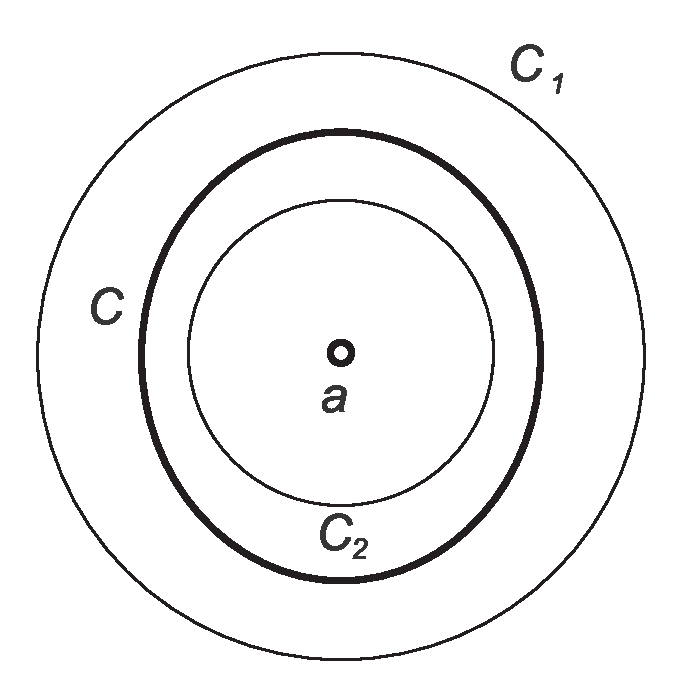
\includegraphics[width=0.35\textwidth]{fig-344.eps}
\caption{Teorema de Laurent}
\label{fig-344}
\end{figure}

Como no caso da s\'{e}rie de Taylor, $f$ pode ser singular em
alguns pontos no exterior de $\mathcal{C}_1$ e constituindo uma
caracter\'{\i}stica nova essencial $f(z)$ pode ser singular em alguns
pontos no interior de $\mathcal{C}_2$.

\begin{theoc}{Teorema de Laurent}{} Se $f$ for anal\'{\i}tica e un\'{\i}voca
sobre duas circunfer\^{e}ncias conc\^{e}ntricas $\mathcal{C}_1$, e
$\mathcal{C}_2$ com centro em $a$ e na coroa por elas limitada,
ent\~{a}o $f$ pode ser representada pela s\'{e}rie de Laurent
\begin{align}
  f(z) & =\sum_{n\geq 0}b_n(z-a)^n+\sum_{n\geq 1}\frac{c_n}{(z-a)^n}\nonumber\\[2ex]
   & =b_0+b_1(z-a)+b_2(z-a)^2+\cdots+\frac{c_1}{z-a}+\frac{c_2}{(z-a)^2}+\cdots\label{laure145:1}
\end{align}
onde
\begin{equation}\label{laure145:2}
b_n= \frac{1}{2\pi j}\int_{\mathcal{C}}\frac{f(w)}{(w -
a)^{n+1}}dw,\qquad  c_n=\frac{1}{2\pi j}\int_{\mathcal{C}}(w -
a)^{n-1}f(w)dw
\end{equation}
\end{theoc}
cada integral sendo calculada no sentido direto em torno de
qualquer caminho fechado simples $\mathcal{C}$, que se situa na
coroa e envolve a circunfer\^{e}ncia menor ver Figura~\ref{fig-344}.

Esta s\'{e}rie converge e representa $f(z)$ na coroa aberta que se
obt\'{e}m da coroa dada aumetando continuamente a circunfer\^{e}ncia
$\mathcal{C}_1$ e diminuindo $\mathcal{C}_2$ at\'{e} que cada uma
delas atinja um ponto onde $f$ seja singular.


\begin{obs} Evidentemente, em lugar de \eqref{laure145:1} e \eqref{laure145:2} podemos escrever
simplesmente
\begin{equation}\label{laure145:3}
f(z)=\sum_{n\in \mathbb{Z}}A_n(z-a)^n
\end{equation}
onde
\begin{equation}\label{laure145:4}
A_n=\frac{1}{2\pi j}\int_{\mathcal{C}}\frac{f(w)}{(w - a)^{n+1}}dw
\end{equation}
\end{obs}

\prova \textbf{do Teorema de Laurent.} Seja $z$ qualquer ponto na
coroa dada. Ent\~{a}o, de acordo com a f\'{o}rmula integral de Cauchy no
caso de um dom\'{\i}nio de conex\~{a}o m\'{u}ltipla segue-se que
\begin{equation}\label{laure145:5}
 f(z)=\frac{1}{2\pi j}\int_{\mathcal{C}_1}\frac{f(w)}{w -
z}dw-\frac{1}{2\pi j}\int_{\mathcal{C}_2}\frac{f(w)}{w - z}dw
\end{equation}
onde ambas as integrais s\~{a}o calculadas no sentido direto. Estas
integrais ser\~{a}o agora transformadas de uma maneira semelhante \`{a}
empregada no desenvolvimento de Taylor. Como $z$ se situa no
interior de $\mathcal{C}_1$ a primeira destas integrais \'{e}
precisamente do mesmo tipo que a integral \eqref{tay141:1}.
Desenvolvendo e estimando o resto, obtemos
\begin{equation}\label{laure145:6}
\frac{1}{2\pi j}\int_{\mathcal{C}_1}\frac{f(w)}{w -
z}dw=\sum_{n\geq 0}b_n(z-a)^n
\end{equation}
onde os coeficientes s\~{a}o dados pela f\'{o}rmula
\begin{equation}\label{laure145:7}
b_n=\frac{1}{2\pi j}\int_{\mathcal{C}_1}\frac{f(w)}{(w -
z)^{n+1}}dw,
\end{equation}
representamos a vari\'{a}vel de integra\c{c}\~{a}o por $w$, j\'{a} que $z$ \'{e}
empregada em $f(z)$, e a integral \'{e} tomada no sentido direto. Como
a n\~{a}o \'{e} um ponto da coroa, as fun\c{c}\~{o}es $f(w)/(w - a)^{n+1}$ s\~{a}o
anal\'{\i}ticas na coroa. Assim, podemos integrar ao longo do caminho
$\mathcal{C}$, em lugar de $\mathcal{C}_1$ sem alterar o valor de
$b_n$.\; Isto demonstra \eqref{laure145:2} para todo $n\geq 0$.

No caso da \'{u}ltima integral, a situa\c{c}\~{a}o \'{e} diferente j\'{a} que $z$ se
situa no exterior de $\mathcal{C}_2$. Em lugar de
\eqref{tay141:3}, temos que
\begin{equation}\label{laure145:8}
 \left|\frac{w - a}{z - a}\right| < 1
\end{equation}
isto \'{e}, temos que desenvolver $1/(w - z)$ em pot\^{e}ncias de $(w -
a)/(z - a)$ para a s\'{e}rie resultante ser convergente. Obtemos
\begin{equation*}
\frac{1}{w- z}= \frac{1}{w - a - (z - a)}= \frac{-1}{(z - a)
\left(1- \frac{w - z}{z - a}\right)}
\end{equation*}

Aplicando a f\'{o}rmula para uma progress\~{a}o geom\'{e}trica finita \`{a} \'{u}ltima
express\~{a}o ela se toma
\begin{align*}
\frac{1}{w - a}&=- \frac{1}{z- a}\left\{1+\frac{w-a}{z-a} +
\left(\frac{w - a}{z- a}\right)^2+\cdots+\left(\frac{w -
a}{z-a}\right)^n\right\}\\[2ex]
&\quad-\frac{1}{z-w}\left(\frac{w - a}{z-a}\right)^{n+1}
\end{align*}

Deste desenvolvimento prontamente obtemos
\begin{align*}
- \frac{1}{2\pi j}&\int_{\mathcal{C}_2}\frac{f(w)}{w -
z}dw \\[2ex]
   &=\frac{1}{2\pi
   j}\left\{\frac{1}{z-a}\int_{\mathcal{C}_2}f(w)dw+\frac{1}{(z-a)^2}
   \int_{\mathcal{C}_2}(w
   -a)f(w)dw+\cdots\right.\\[2ex]
   &\left.+ \frac{1}{(z-a)^{n+1}}\int_{\mathcal{C}_2}(w -
a)^{n}f(w)dw\right\}+R^*_n(z);
\end{align*}
nesta representa\c{c}\~{a}o o \'{u}ltimo termo \'{e} da forma
\begin{equation}\label{laure145:9}
 R_n(z)= \frac{1}{2\pi j(z - a)^{n+1}}\int_{\mathcal{C}_2} \frac{(w -a)^{n+1}}{z-w}
 f(w)dw
\end{equation}

Nas integrais do segundo membro podemos substituir a
circunfer\^{e}ncia $\mathcal{C}_2$ pelo anteriormente mencionado
caminho $\mathcal{C}$, sem alterar seus valores. Assim, o teorema
de Laurent fica demonstrado se provarmos que
\begin{equation}\label{laure145:10}
 \lim_{n\to\infty} R_n(z) = 0.
\end{equation}

Demonstremos \eqref{laure145:10}. Como $z - w \neq 0$ e $f$ \'{e}
anal\'{\i}tica na coroa e sobre $\mathcal{C}_2$, o valor absoluto da
express\~{a}o $f(w)/(z - w)$ \'{e} limitado, digamos
\begin{equation*}
\left|\frac{f(w)}{z - w}\right| < \tilde{M},\quad \text{para
qualquer } \quad w \in \mathcal{C}_2.
\end{equation*}

Aplicando estimativa de valor absoluto a uma integral de linha \`{a}
\eqref{laure145:9}, e representando o comprimento de
$\mathcal{C}_2$ por $l$, obtemos
\begin{equation*}
|R_n^*(z)| < \frac{1}{2\pi|z-a|^{n+1}} |w - a|^{n+1}\tilde{M}l =
\frac{\tilde{M} l}{2\pi} \left|\frac{w - a}{z - a}\right|^{n+1}
\end{equation*}

De \eqref{laure145:8} conclu\'{\i}mos que a express\~{a}o da direita se
aproxima de zero \`{a} medida que $n$ se aproxima do infinito. Assim,
\eqref{laure145:10} fica demonstrada. A representa\c{c}\~{a}o
\eqref{laure145:1} com coeficientes \eqref{laure145:2} fica
estabelecida na coroa dada.

Finalmente, vamos demonstrar a converg\^{e}ncia de \eqref{laure145:1}
na coroa aberta caracterizada no fim do teorema.

Representamos as somas das duas s\'{e}ries em \eqref{laure145:1} por
$g(z)$ e $h(z)$ e os raios de $\mathcal{C}_1$ e $\mathcal{C}_2$
por $r_1$ e $r_2$ respectivamente. Assim, $f = g + h$. A primeira
s\'{e}rie \'{e} uma s\'{e}rie de pot\^{e}ncias. De vez que ela converge na coroa,
ela deve convergir em todo o disco limitado por $\mathcal{C}_1$ e
$g$ \'{e} anal\'{\i}tica no disco.

Fazendo $Z = 1/(z - a)$, a \'{u}ltima s\'{e}rie se transforma numa s\'{e}rie
de pot\^{e}ncias em $Z$. A coroa $r_2 <| z - a | < r_1$, ent\~{a}o
corresponde \`{a} coroa $1/r_1 < | Z| < 1/r_2$, a nova s\'{e}rie converge
na coroa e, portanto, em todo o disco $| Z | < 1/r_2$. Agora, como
o disco corresponde a $|z- a| > r_2$, o exterior de
$\mathcal{C}_2$, a s\'{e}rie dada converge para todo $z$ no exterior
de $\mathcal{C}_2$ e $h$ \'{e} anal\'{\i}tica para todos estes valores de
$z$.

Como $f = g + h$, segue-se que $g$ deve ser singular em todos
aqueles pontos no exterior de $\mathcal{C}_2$, onde $f$ \'{e}
singular, e $h$ deve ser singular em todos aqueles pontos no
interior de $\mathcal{C}_2$ onde $f$ \'{e} singular. Conseq\"{u}entemente,
o raio de converg\^{e}ncia da primeira s\'{e}rie \'{e} igual \`{a} dist\^{a}ncia da
singularidade de $f$, no exterior de $\mathcal{C}_1$ que \'{e} mais
pr\'{o}xima de $a$. Semelhantemente, a segunda s\'{e}rie converge para
todo $z$ no exterior de uma circunfer\^{e}ncia com centro em a cujo
raio \'{e} igual \`{a} dist\^{a}ncia m\'{a}xima das singularidades de $f$ no
interior de $\mathcal{C}_2$.

O dom\'{\i}nio comum a ambos estes dom\'{\i}nios \'{e} a coroa aberta caracterizada
no fim do teorema; assim a demonstra\c{c}\~{a}o fica completa.

Segue-se que, se $f$ for anal\'{\i}tica no interior de
$\mathcal{C}_2$, a s\'{e}rie de Laurent se reduz \`{a} s\'{e}rie de Taylor de
$f$ com centro em $a$. Realmente, aplicando o teorema integral
de Cauchy a \eqref{laure145:2}, vemos que, neste caso, todos os
coeficientes das pot\^{e}ncias negativas em \eqref{laure145:1} s\~{a}o
zero.

Al\'{e}m disso, se $z = a$ for o \'{u}nico ponto singular de $f$ em
$\mathcal{C}_2$, ent\~{a}o o desenvolvimento de Laurent
\eqref{laure145:1} converge para todo $z$ em $\mathcal{C}_1$
exceto em $z = a$. Este caso ocorre freq\"{u}entemente e possui,
portanto, particular import\^{a}ncia.

A s\'{e}rie de Laurent de uma dada fun\c{c}\~{a}o anal\'{\i}tica $f$ em sua
coroa de converg\^{e}ncia \'{e} \'{u}nica (veja os exerc\'{\i}cios desta se\c{c}\~{a}o).
Entretanto, $f$ pode possuir s\'{e}ries de Laurent diferentes em
duas coroas com o mesmo centro (veja  Exemplo~\ref{xe145:2},
abaixo).

A unicidade \'{e} importante, porque a s\'{e}rie de Laurent em geral n\~{a}o \'{e}
obtida empregando \eqref{laure145:2} para calcular os
coeficientes, mas por v\'{a}rios outros m\'{e}todos. Alguns destes m\'{e}todos
s\~{a}o ilustrados nos exemplos que se seguem. Se uma s\'{e}rie de Laurent
for determinada por um destes processos, ela deve ser a s\'{e}rie de
Laurent da fun\c{c}\~{a}o dada na coroa fixada. \qed

\begin{exer}\label{xe145:1}
Obtenha a s\'{e}rie de Laurent de $z^2e^{1/z}$ com centro em $0$.
\end{exer}

 \solo Pode ser obtida de \eqref{elem142:2}. Substituindo $z$ por $1/z$ naquela
s\'{e}rie vem
\begin{align*}
  z^2e^{1/z} &=z^2\left( 1+\frac{1}{1!z}+\frac{1}{2!z^2}+\cdots \right) \\[2ex]
   &=z^2  + z + \frac{1}{2} + \frac{1}{3!z}+\frac{1}{4!z}+\cdots,  \qquad|z| >0.
\end{align*}

Assim obtemos a s\'{e}rie de Laurent.\hfill \(\lozenge\)

\begin{exer}\label{xe145:2}
Determinar todas as s\'{e}ries de Laurent de $f(z) =
1/(1-z^2)$ com centro em $z = 1$.
\end{exer}

\solo  Temos $1 - z^2= -(z - 1) (z + 1)$. Empregando a s\'{e}rie
geom\'{e}trica
\begin{equation*}
 \frac{1}{1-q} =\sum_{n\geq 0}q^n\qquad |q|<1,
\end{equation*}
empregamos
\begin{align}
  \frac{1}{z+1} &= \frac{1}{2+(z-1)}=\frac{1}{2}\frac{1}{\left[1-\left(-\frac{z-1}{2}
  \right)\right]}\nonumber\\[2ex]
   &= \frac{1}{2}\sum_{n\geq 0}\left(-\frac{z-1}{2} \right)^n=\sum_{n\geq 0}
   \frac{(-1)^{n+1}}{2^{n+1}}(z-1)^n\label{laure145:a}
\end{align}

esta s\'{e}rie converge no disco $|(z - 1)/2| < 1$, isto \'{e}, $|z-1| <
2$. Semelhantemente,
\begin{align}
\frac{1}{z+1} &=
\frac{1}{(z-1)+2}=\frac{1}{z-1}\frac{1}{\left[1+\left(\frac{2}{z-1}\right)\right]}
\nonumber\\[2ex]
&= \frac{1}{z-1}\sum_{n\geq 0}\left(-\frac{2}{z-1} \right)^n=\sum_{n\geq 0}
   \frac{(-2)^{n}}{(z-1)^{n+1}}\label{laure145:b}
\end{align}

esta s\'{e}rie converge para $|2/(z - 1)| < 1$, isto \'{e}, $|z - 1|>2$.
Portanto, de \eqref{laure145:a} obtemos
\begin{align*}
f(z) &=\frac{-1}{(z-1)(z+1)}=\sum_{n\geq 0}\frac{(-1)^{n+1}}{2^{n+1}}(z-1)^{n-1}\\[2ex]
   &=\frac{-1/2}{z-1}+\frac{1}{4}-\frac{1}{8}(z-1)+\frac{1}{16}(z-1)^2-+\cdots;
\end{align*}

esta s\'{e}rie converge no dom\'{\i}nio $0 < | z - 1| < 2$. De
\eqref{laure145:b}
\begin{equation*}
f(z) =-\sum_{n\geq
0}\frac{(-2)^{n}}{(z-1)^{n+2}}=-\frac{1}{(z-1)^2}+\frac{2}{(z-1)^3}-
\frac{4}{(z-1)^4}+-\cdots,
\quad |z-1|>2
\end{equation*}

Portanto existem varias s\'{e}ries de Laurent.\hfill \(\lozenge\)

\begin{exer}\label{xe145:3}
Utilizando o exerc\'{\i}cio do fim da se\c{c}\~{a}o s\'{e}ries de Taylor das
fun\c{c}\~{o}es elementares, obtenha a s\'{e}rie de Laurent da fun\c{c}\~{a}o $\cot
z$.
\end{exer}

\solo Com efeito,
\begin{equation*}
\cot(z)
=\frac{1}{z}-\frac{1}{3}z-\frac{1}{45}z^3-\frac{2}{945}z^5-\cdots,\quad
0<|z|<\pi.
\end{equation*}

Obtendo a s\'{e}rie pedida. \hfill \(\lozenge\)

%%%
\section*{Exerc\'{\i}cios Propostos} 
%%%
Resolver os seguintes exerc\'{\i}cios sobre fun\c{c}\~{o}es complexas
\begin{enumerate}[label=(\arabic*)]
\item Desenvolver as seguintes fun\c{c}\~{o}es em s\'{e}ries de Laurent;
convergentes para a desigualdade $0 <| z |<R$ e determinar
precisamente a regi\~{a}o de converg\^{e}ncia.
\begin{tasks}[](2)
\rm{(a)}&\quad \frac{e^{-z}}{z^3}
\rm{(b)}&\quad \frac{e^{1/z^2}}{z^6}
\rm{(c)}&\quad \frac{\cos(2z)}{z^2}
\rm{(d)}&\quad \frac{1}{z^4(1+z)}
\rm{(e)}&\quad \frac{1}{z^2(1-z^2)}
\rm{(f)}&\quad \frac{1}{z^2(z-3)}
\rm{(g)}&\quad \frac{\senh(3z)}{z^3}
\rm{(h)}&\quad \frac{1}{z^4+z^8}
\end{tasks}

\item Demonstrar que o desenvolvimento de Laurent de uma dada fun\c{c}\~{a}o
anal\'{\i}tica em uma dada coroa \'{e} \'{u}nico.

\item Determinar todas as s\'{e}ries de Taylor e de Laurent com centro
em $z = a$ e determinar precisamente as regi\~{o}es de converg\^{e}ncia:
\begin{tasks}[](2)
\rm{(a)}&\quad \dfrac{1}{z^2+1}, \quad  a=-j 
\rm{(b)}&\quad \dfrac{1}{z^4}, \quad a=1
\rm{(c)}&\quad \dfrac{1}{z^3}, \quad a=j 
\rm{(d)}&\quad \dfrac{7z^2+9z-18}{z^3-9z},quad  a=0
\rm{(e)}&\quad \dfrac{4z^2+2z-4}{z^3-4z},\quad a=2 
\rm{(f)}&\quad \dfrac{\sen(z)}{(z-\pi/4)},\quad a=\pi /4
\end{tasks}
\end{enumerate}

%%%%%
\section{Comportamento de Fun\c{c}\~{o}es no Infinito}
%%%%
Veremos na pr\'{o}xima se\c{c}\~{a}o que a s\'{e}rie de Laurent pode ser empregada
para classificar as singularidades das fun\c{c}\~{o}es anal\'{\i}ticas. Dentro
desta ordem de id\'{e}ias tamb\'{e}m consideraremos o comportamento das
fun\c{c}\~{o}es anal\'{\i}ticas $f$ quando $|z|$ se aproxima do infinito.

Para investigar o comportamento de uma fun\c{c}\~{a}o $f$ para $|z|$
grande, parece natural introduzir uma nova vari\'{a}vel $w$ fazendo
$z=1/w$ porque, ent\~{a}o, $|z|$ grande corresponde a $|w|$ pequeno, e
$|z|$ vai ao infinito  corresponde a $|w|$ vai ao zero.

A transforma\c{c}\~{a}o $w = 1/z$ foi considerada  no plano complexo
prolongado que foi obtido vinculando ao plano complexo finito, um
ponto impr\'{o}prio (o ponto no infinito). Podemos ent\~{a}o fazer $z
=\infty$ corresponder a $w = 0$ (e $w =\infty$ corresponder a $z =
0$). O procedimento de prolongar o plano complexo pode ser tamb\'{e}m
motivado pela considera\c{c}\~{a}o geom\'{e}trica simples que se segue.

A representa\c{c}\~{a}o usual dos n\'{u}meros complexos $\mathbb{C}$ no plano
complexo \'{e} conveniente enquanto os valores absolutos dos n\'{u}meros
n\~{a}o forem dema, siado grandes. Para $| z |$ grande a situa\c{c}\~{a}o se
toma inconveniente, e neste caso, podemos preferir uma
representa\c{c}\~{a}o dos n\'{u}meros complexos sobre uma esfera, a qual foi
sugerida por Riemann e se obt\'{e}m da seguinte maneira.

Seja $\mathcal{S}$ uma esfera de di\^{a}metro um que tangencia o plano
complexo $ \mathbb{C} $ na origem, ver Figura~\ref{fig-345}.
\begin{figure}[H]
\centering
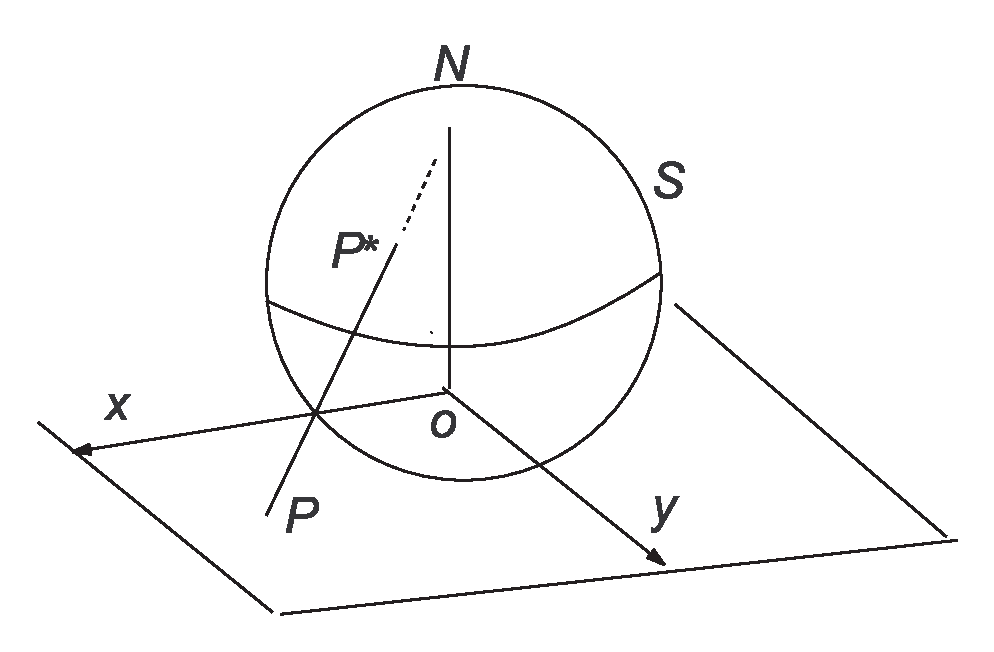
\includegraphics[width=0.5\textwidth]{fig-345.eps}
\caption{Esfera de Riemann} \label{fig-345}
\end{figure}

Seja $N$ o P\'{o}lo Norte de $\mathcal{S}$ (o ponto diametralmente
oposto ao ponto de contato entre a esfera e o plano). Seja $P$
qualquer ponto no plano complexo. Ent\~{a}o a reta definida por $P$ e
$N$ intercepta $\mathcal{S}$ no ponto $P^*$. Fazemos $P$ e $P^*$
corresponderem um ao outro. Desta maneira obtemos uma
correspond\'{e}ncia entre os pontos do plano complexo e os pontos
sobre $S$, e $P^*$ \'{e} a imagem do ponto $P$ nesta representa\c{c}\~{a}o. Os
n\'{u}meros complexos, primeiramente representados no plano, s\~{a}o
agora, representados por pontos sobre $\mathcal{S}$. A cada $z$
corresponde um ponto sobre $\mathcal{S}$. Reciprocamente, cada
ponto sobre $\mathcal{S}$ representa um n\'{u}mero complexo $z$,
exceto o ponto $N$ que n\~{a}o corresponde a nenhum ponto no plano
complexo.

Se, entretanto, introduzirmos o ponto impr\'{o}prio $z
=\infty$  e fizermos este ponto corresponder a $N$, a
representa\c{c}\~{a}o se transforma em uma representa\c{c}\~{a}o un\'{\i}voca do plano
prolongado sobre $\mathcal{S}$. A esfera $\mathcal{S}$ \'{e} chamada a
esfera dos n\'{u}meros de Riemann. A representa\c{c}\~{a}o particular que
empregamos \'{e} chamada uma proje\c{c}\~{a}o estereogr\'{a}fica.

Evidentemente, a circunfer\^{e}ncia unit\'{a}ria \'{e} representada sobre, o
``equador'' de $\mathcal{S}$. O interior da circunfer\^{e}ncia unit\'{a}ria
corresponde ao ``Hemisf\'{e}rio Sul" e o exterior ao ``Hemisf\'{e}rio
Norte'' Os n\'{u}meros $z$, cujos valores absolutos s\~{a}o grandes, se
situam pr\'{o}ximo ao P\'{o}lo Norte $N$. Os eixos dos $x$ e dos $y$ (e,
em geral, as retas que passam pela origem) s\~{a}o representadas sobre
os ``meridianos'', enquanto as circunfer\^{e}ncias com centro na origem
s\~{a}o representadas sobre os ``paralelos''.

Podemos demonstrar que qualquer circunfer\^{e}ncia ou reta no plano $\mathbb{C}$ \'{e}
representada sobre uma circunfer\^{e}ncia em $ \mathcal{S}$; al\'{e}m
disso, podemos provar que a \textit{proje\c{c}\~{a}o estereogr\'{a}fica} \'{e} conforme,
isto \'{e}, duas curvas quaisquer que se interceptam possuem imagens
cujo \^{a}ngulo de interse\c{c}\~{a}o \'{e} igual ao \^{a}ngulo de interse\c{c}\~{a}o das
curvas.

Dada uma fun\c{c}\~{a}o $f$ a ser investigada para $| z |$ grande,
podemos fazer $z =1/w$ e investigar $f(z) = f(1/w)\equiv g(w)$ em
uma vizinhan\c{c}a de $w = 0$. Definimos
\begin{equation*}
g(0) = \lim_{w\to 0} g(w),
\end{equation*}
e dizemos que $f(z)b$ \'{e} anal\'{\i}tica ou singular no infinito,
conforme $g(w)$ seja anal\'{\i}tica ou singular, respectivamente, em $w
= 0$.

\begin{exer}\label{infi146:1}
A fun\c{c}\~{a}o $f(z) = 1/z^2$ \'{e} anal\'{\i}tica no infinito, j\'{a} que $g(w) =
f(1/w)=w^2$ \'{e} anal\'{\i}tica em $w=0$. A fun\c{c}\~{a}o $f(z) = z^3$ \'{e} singular
no infinito porque $g(w) =f(1/w) = 1/w^2$ \'{e} singular em $w=0$. A
fun\c{c}\~{a}o exponencial $e^z$ \'{e} singular no infinito j\'{a} que $e^{1/w}$ \'{e}
singular em $w = 0$. Semelhantemente, as fun\c{c}\~{o}es trigonom\'{e}tricas
$\sen z$ e $\cos z$ s\~{a}o singulares no infinito.
\end{exer}

Seja $f(z)$ anal\'{\i}tica no exterior de uma circunfer\^{e}ncia
$\mathcal{C}$, digamos, no dom\'{\i}nio $|z - a| > R$, e tamb\'{e}m no
infinito. Se fizermos
\begin{equation*}
z= \frac{1}{w} + a,\quad \text{ ent\~{a}o }\quad z - a = \frac{1}{w}
\end{equation*}
e
\begin{equation*}
  f(z)=f\left(\frac{1}{w}+a \right)\equiv h(w)
\end{equation*}

\'{e} anal\'{\i}tica no disco $| w | < 1/R$. Seja a s\'{e}rie de Maclaurin de
$h(w)$
\begin{equation*}
h(w) =\sum_{n\geq 0}c_nw^n= c_o + c_1w + c_2w_2 + \cdots\qquad |w|
< \frac{1}{R}
\end{equation*}

Ent\~{a}o, substituindo $w = 1/(z - a)$ obtemos a s\'{e}rie de Laurent
\begin{equation}\label{infi146:2}
f(z) =\sum_{n\geq 0}\frac{c_n}{(z-a)^n}=c_o + \frac{c_1}{(z - a)}
+ \frac{c_2}{(z - a)^2}+\cdots,\quad |z-a|>R.
\end{equation}

Obtendo o que desejavamos.\hfill \(\lozenge\)

%%%
\section*{Exerc\'{\i}cios Propostos}
%%%% 
Resolver as quest\~{o}es a seguir sobre as fun\c{c}\~{o}es anal\'{\i}ticas
\begin{enumerate}[label=(\arabic*)]
\item As fun\c{c}\~{o}es seguintes s\~{a}o anal\'{\i}ticas no infinito ou n\~{a}o?
\begin{align*}
\rm{(a)}&\quad z^2 + z^{-2}   &\rm{(b)}&\quad  z^{-3}+z^{-1}\\[2ex]
\rm{(c)}&\quad e^z,\quad e^{z^2},\quad e^{-z} &\rm{(d)}& \quad e^{1/z},\quad e^{1/z^2}\\[2ex]
\rm{(e)}&\quad \cos(z),\quad \sen(z)  &\rm{(f)}&\quad \cosh(z),\quad\senh(z)\\[2ex]
\rm{(g)}&\quad ze^{1/z} &(h)&\quad 1/(z^2-3z)
\end{align*}

\item Descrever e esbo\c{c}ar as imagens das regi\~{o}es seguintes sobre a
esfera dos, n\'{u}meros de Riemann.
\begin{align*}
\rm{(a)}&\quad \textrm{Re}\; z\le 0  &\rm{(b)}&\quad \textrm{Im}\; z\geq 0\\[2ex]
\rm{(c)}&\quad  |z|\geq 5 &\rm{(d)}&\quad |z|\le 2\\[2ex]
\rm{(e)}&\quad 1/2\le |z|\le 2  &\rm{(f)}&\quad |z|\le 3,\quad |arg\; z|<\pi/2
\end{align*}

\item Empregando o m\'{e}todo descrito no fim desta se\c{c}\~{a}o, mostrar que
\begin{equation*}
\frac{1}{z^4}=\sum_{n\geq 0}{-4\choose n}(z-1)^{-n-4} =
\frac{1}{(z-1)^4}-\frac{4}{(z-1)^5}+\cdots,\qquad |z-1|>1
\end{equation*}
\end{enumerate}

%
\chapter{Sequências e Séries de Funções}

\section{Sequência de Funções: Converg\^encia  Pontual}
%%%
O tipo mais natural de converg\^encia para uma sucess\ao\ de fun\coes\ provavelmente \'e pontual 
(ou simples) converg\^encia, definido como segue.

\begin{defic}{Convergência Pontual de Sequência de Funções}{} 
Uma \seq\ de funções de $\mathbb{R}^p$ em
$\mathbb{R}^m$ é uma função cujo domínio é o conjunto dos interios
positivos e cuja imagem é um conjunto de funções de $\mathbb{R}^p$
em $\mathbb{R}^m$. A \seq\ de funções de $\mathbb{R}^p$ em
$\mathbb{R}^m$ é representada por $\{f_n\}$.

Para cada ponto $x$ do domínio de todos os termos da \seq\ de
funções $\{f_n\}$, existe uma \seq\ de pontos $\{f_n(x)\}$. Se
$\{f_n(x)\}$ converge para cada ponto $x$ de um conjunto
$\mathcal{E}$ e fazemos
\begin{equation*}
    f(x)=\lim_{n\to \infty}f_n(x),
\end{equation*}
então dizemos que $\{f_n\}$ \textbf{converge pontualmente}  a $f$
sobre $\mathcal{E}$.
\end{defic}

De forma equivalente em dimensões menores. Uma \seq\ $\{f_n\}$
onde cada elemento é uma função $f_n\colon I\subseteq
\mathbb{R}\to \mathbb{R}$, \textit{converge pontualmente em I} se
existe o limite
\begin{equation*}
  \lim_{n\to\infty}f_n(x_{0})
\end{equation*}
relativamente a cada $x_{0}$ de $I$.


\begin{exer} 
Seja $f_n(x) =x^n,\quad 0\leq x\leq 1$, $n= 1,\; 2,\;  3,\ldots$
Verifique a convergência pontual.
\end{exer}

\solo Para $0\leq x_{_{0}}<1$ temos
\begin{equation*}
  \lim_{n\to\infty} f_n(x_{_{0}}) = \lim_{n\to\infty} x_{_{0}}^n=0,
\end{equation*}
ao passo que, quando $x =1$, $\dst{\lim_{n\to\infty}f_n(1) = 1}$.

A sequência dada, portanto, converge pontualmente no intervalo $0
\leq  x \leq 1$ para a função
\begin{equation*}
  f(x) =
    \begin{cases}
      0 & \quad \text{ se } \quad 0\leq x < 1 \\[2ex]
      1 & \quad \text{ se }\quad x=1
    \end{cases}
\end{equation*}
veja o lado esquerdo da Figura~\ref{fig-1116-5}.
\begin{figure}[H]
\centering
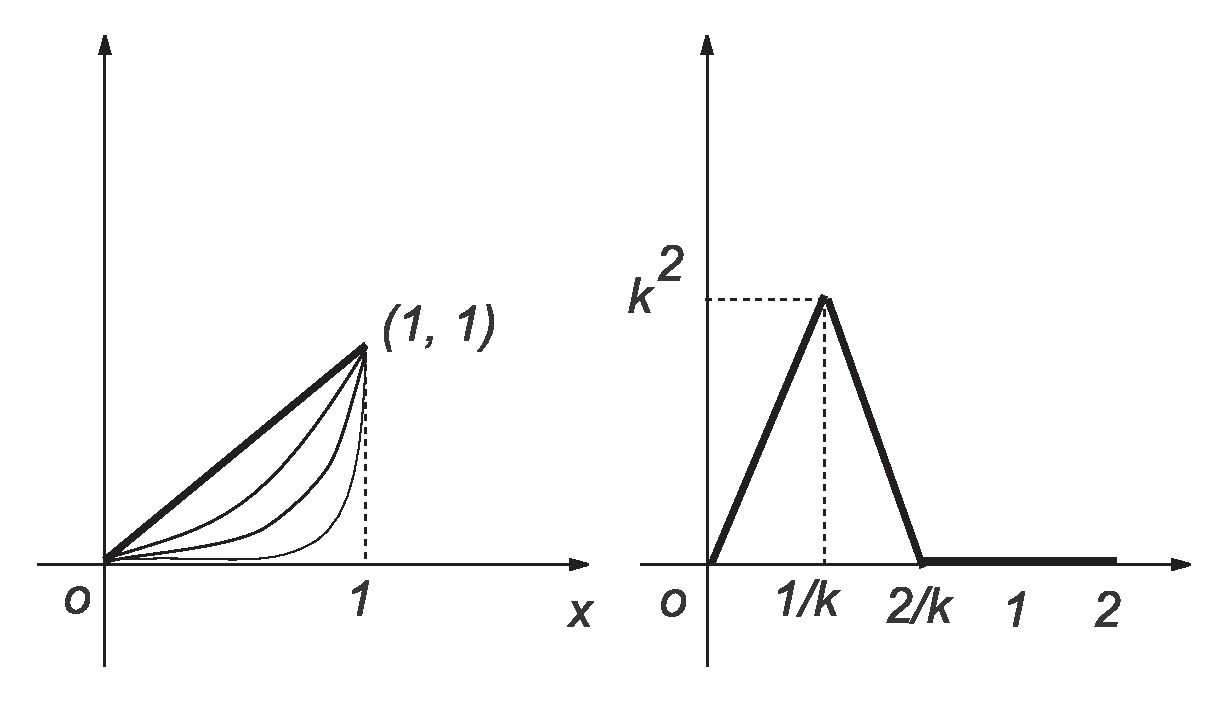
\includegraphics[width=0.6\textwidth]{fig-1116-5.eps}
\caption{Convergência Pontual}
\label{fig-1116-5}
\end{figure}

Observemos que, enquanto cada uma das $f_n$ é contínua no
intervalo inteiro $0 \leq x \leq 1$, a função limite $f$ não é
contínua neste intervalo (ela é descontínua em $x = 1$).

Em no caso geral a \seq\ $\{x^n\}$ para $x\in \mathbb{R}$ converge
para zero se $x\in ]-1, \; 1[$, converge para um se $x=1$, e diverge
se $x\in ]-\infty, \; -1]\cup ]1, \; \infty[$. Portanto a \seq\ converge
pontualmente sobre $\mathcal{E}=]-1,\; 1]$ para a função $f$ onde
\begin{equation*}
  f(x) =
    \begin{cases}
      0 & \text{ se } \quad -1< x < 1 \\[2ex]
      1 & \text{ se } \quad x=1
    \end{cases}
\end{equation*}

Observamos que cada termos da \seq\ de funções é uma função
contínua, a função limite $f$ não é contínua.\qed

Mesmo que a convergência uniforme é suficiente para garantir que o
limite de uma \seq\ de funções contínuas é contínua, não é uma
condição necessária para este resultado. No seguinte exemplo, a
\seq\ de funções contínuas não converge uniformemente e mesmo
assim a função limite $f$ é contínua

\begin{exer}\label{ex1116-2}
Seja a \seq\ $\{f_k\}$ onde cada função esta definida em $0\leq x
\leq 2$, onde
\begin{equation*}
    f_1(x)=k^2,\quad 0\le x\le 2
\end{equation*}
e para $k\ge 2$ seja
\begin{equation*}
  f_k(x) =
    \begin{cases}
      k^3x & \text{ se}, \quad 0\le x \le 1/k \\[2ex]
      2k^2-k^3x & \text{ se},\quad 1/k<x\le 2/k\\[2ex]
      0 &\text{ se}, \quad  2/k<x\le 2
    \end{cases}
\end{equation*}
cujo gráfico esta indicado no lado direito da
Figura~\ref{fig-1116-5}. Discutir a convergência pontual.
\end{exer}

\solo Evidentemente, $f_k(0)= 0$ para todo $k$, donde
$\dst{\lim_{n\to\infty}f_k(0) = 0}$. Mais ainda, se $0 < x_o\leq
2$, então existe algum valor de $k$, digamos $N$, tal que $2/N <
x_o$ e, assim, $f_k(x_o) = 0$ para todo $k \geq N(\varepsilon)$.

Portanto, $\dst{\lim_{k\to\infty} f_k(x_o) = 0}$, e concluímos que
$\{f_k(x)\}$ converge pontualmente para a função identicamente
nula no intervalo $0\leq x \leq 2$ e portanto contínua. Porém a
convergência não é uniforme, pois para qualquer $k$ se $x=1/k$,
então $|f_k(x)-f(x)|=k^2$.

Desta vez, a sequência de funções contínuas converge para um
\textit{limite contínuo}. Apesar disto, as funções $f_k$, não
importa a que distância elas estejam na sequência, podem diferir,
por grande margem, da função limite $f(x)\equiv 0$. Por
conseguinte, os elementos da sequência não são ``aproximações"\;
do limite da sequência no sentido que se espera do termo. E as
integrais dos termos da sequência refletem êste comportamento
peculiar, deixando de tender para a integral da função limite
$f(x)$.

De fato, $\dst{\int_0^2f(x)dx = 0}$, enquanto que
\begin{equation*}
  \int_0^2f_k(x)dx =\frac{1}{2}\cdot\frac{2}{k}\cdot k^2=k
\end{equation*}
e tendem para infinito, não-zero, quando $k$ vai ao infinito.\hfill \(\lozenge\)

A fim de eliminar esta espécie de comportamento, introduzamos
agora um tipo de convergência mais forte, denominada
\textit{convergência uniforme}.

%%%%
\section{Sequência de Funções: Convergência Uniforme}
%%%%

Muitas das fun\c c\~oes que n\'os estudamos serão definidas por
meio de sucess\oes\ infinitas ou s\'eries. Para estudar tais
fun\coes\ precisamos entender o conceito de converg\^encia
uniforme de uma sucess\ao\ ou s\'erie de  fun\coes\ (cont\ii
nuas). Para lidar efetivamente com situa\coes\ concretas e
exemplos, nós também consideraremos v\'arios importantes testes de
converg\^encia uniforme.

Talvez o teste mais \'util em exemplos particulares s\ao\ o
M-teste de Weierstrass para s\'eries. Outro teste \'e o Critério
de Cauchy que \'e principalmente de uso te\'orico. N\'os tamb\'em
inclu\ii mos os testes mais refinados de Dirichlet e Abel.

Em conexão  com a converg\^encia uniforme introduzimos um espa\co\
cujos pontos s\ao\ fun\coes.\ Neste espa\co\ n\'os introduzimos
uma norma e mostramos  que a converg\^encia nesta esta norma \'e
precisamente a converg\^encia uniforme. O espa\co\ é completo no
sentido que sucess\oes\ de Cauchy convergem. Uma segunda
propriedade b\'asica deste espaço, chamada de teorema de
Arzela-Ascoli, estabelece a compacidade de um subconjunto (no
sentido de possuir a propriedade de Bolzano-Weierstrass). Outro
resultado importante, chamado de teorema o Stone-Weierstrass
também é provado. Este teorema permite  aproximar fun\coes\
cont\ii nuas através de polin\^omios, ou por fun\coes\ de outras
classes apropriadas. Finalmente, algumas aplica\coes\ desta
maquinaria s\ao\ fornecidas para\ equa\coes\  diferenciais e
integrais.

\begin{defic}{}{} Uma sequência de funções $\{f_n\}$ \textbf{converge
uniformemente} para a função $f$ sobre o conjunto $\mathcal{E}=[a,
b]$, se para todo $\varepsilon > 0$ existe um número inteiro positivo
$N= N(\varepsilon) \in \mathbb{N}$, dependente de $\varepsilon$ mas não 
de $x$, tal que para todo $x\in \mathcal{E}$
\begin{equation*}
  |f_n(x) - f(x)|< \varepsilon\quad \text{ sempre que }\quad  n>
  N(\varepsilon).
\end{equation*}
\end{defic}

É claro, evidentemente, que, se $\{f_n\}$ converge uniformemente
para $f$ em $a\leq x\leq b$, então ela também converge
\textit{pontualmente} para $f$ neste intervalo. Porém a
convergência pontual de $\{f_n\}$ para $f$ sobre $\mathcal{E}$ não
implica a convergência uniforme da \seq\ para $f$ sobre
$\mathcal{E}$.

Realmente podemos alcançar a convergência uniforme
a partir da convergência pontual se e somente se para cada
$\varepsilon>0$ existe um conjunto de números $\{N(x)\colon x\in
\mathcal{E}\}$ superiormente limitado (acotado). Se $\{f_n\}$ converge
pontualmente para $f$ sobre $\mathcal{E}$ e $N$ é uma cota
superior (majorante) do conjunto $\{N(x)\colon x\in \mathcal{E}\}$, então para
todo $x\in \mathcal{E}$
\begin{equation*}
    |f_n(x)-f(x)|<\varepsilon\quad\text{sempre que }\quad n>N.
\end{equation*}

Assim, $\{f_n\}$ é uniformemente convergente para $f$ sobre
$\mathcal{E}$. Além disso, se $\{f_n\}$ é uniformemente
convergente a $f$ sobre $\mathcal{E}$ e $N$ corresponde para
$\varepsilon>0$, então para cada $x\in \mathcal{E}$ podemos tomar
$N(x)=N$ e o conjunto $\{N(x)\colon x\in \mathcal{E}\}$ ficara
(acotado) limitado superiormente por $N$.

No caso, da convergência uniforme, pode-se escolher $n$ de
modo tal que
\[
f(x) -\varepsilon<f_n(x)<f(x) +\varepsilon
\]
para cada $x$ no intervalo $a\leq x \leq b$. Portanto, $f_n$ é uma
aproximação de $f$ com diferença inferior a $\varepsilon$, no
intervalo todo, como o mostra a Figura~\ref{fig-1116-7}.
\begin{figure}[H]
\centering
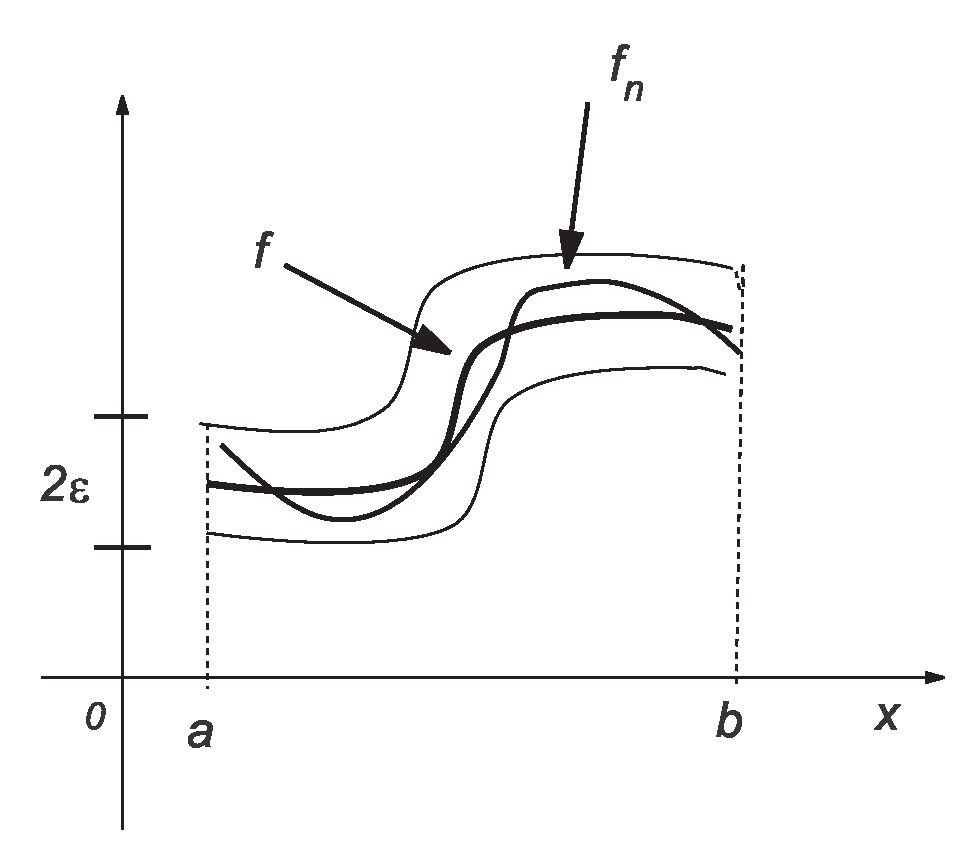
\includegraphics[width=0.45\textwidth]{fig-1116-7.eps}
\caption{Convergência Uniforme}
\label{fig-1116-7}
\end{figure}

Observamos, no Exemplo~\ref{ex1116-2}, que no caso de convergência
pontual nenhum dos termos da sequência é, necessáriamente, uma
aproximação da função limite, nesse sentido.

\begin{exer}
Escrever cuidadosamente as defini\coes\ de converg\^encia pontual
(ou simples) e converg\^encia uniforme. Com as defini\coes\
anteriores verifique a seguinte implicação,
\begin{center}
Converg\^encia uniforme $\ent$ Converg\^encia Pontual
\end{center}
\end{exer}

\solo A \seq\ de fun\coes\ $u_n\colon I\subset \R\to \R$ converge
pontualmente para a $u\colon I\subset \R\to \R $ ou $(u_n\to u)$
sobre o conjunto $I\subset \R$ se para cada $\mathbf{\varepsilon}$
e para cada $x\in I$ existe um n\'umero, $N=
N(x,\mathbf{\varepsilon})$ tal que,
\begin{equation*}
|u_n(x)-u(x)|<\mathbf{\varepsilon}\quad \text{ sempre que } \quad n>N.
\end{equation*}


Definimos a converg\^encia uniforme: a \seq\
de fun\coes\ $u_n\colon I\subset \R\to \R$ converge uniformemente
a $u\colon I\subset \R\to \R$ ($u_n\rightrightarrows u$) sobre o
conjunto $I\subset \R$ se para cada $\varepsilon$ existe um
n\'umero, $N= N(\mathbf{\varepsilon})$ tal que se para todo $x\in
I$,
\begin{equation*}
|u_n(x)-u(x)|<\mathbf{\varepsilon}\quad \text{ sempre que } \quad n>N.
\end{equation*}

Observamos que $u_n \uni u (\uni)$ implica $u_n \to u$. Pois se funciona para todo $x\in I$, em particular para cada $x\in I$, 
e para $\mathbf{\varepsilon}>0$ dado,  temos $N=N(x, \mathbf{\varepsilon})$ tal que
\begin{equation*}
|u_n(x)-u(x)|<\mathbf{\varepsilon}\quad \text{sempre que}\quad n>N.
\end{equation*}

Assim obtemos a converg\^encia simples, $u_n\to u$. \qed

No contexto da convergência uniforme temos que:
\begin{equation*}
    \text{Limite uniforme} = \text{Limite pontual}
\end{equation*}

Lembremos também que convergência pontual não implica convergência uniforme como será ilustrado no seguinte contra-exemplo;

\begin{exer}
Seja a seguinte \seq de funções $\{f_n\}$ aonde cada termo é
\begin{equation*}
    f_n(x)=\frac{nx}{1+(nx)^2},\qquad x\in \mathbb{R}.
\end{equation*}

Mostre que não converge uniformemente em qualquer intervalo
$[a,b]$ tendo o zero como seu ponto interior.
\end{exer}

\solo Como podemos ver, aplicando resultados de convergência
simples, a \seq $\{f_n\}$ converge pontualmente com limite pontual
$f$ tal que
\begin{equation*}
    f(x)=0,\qquad x\in \mathbb{R}.
\end{equation*}

A seguir mostramos que a convergência não é uniforme em qualquer
intervalo $[a,b]$ que contenha o ponto zero como ponto interior.

Suponhamos que a convergência seja uniforme sobre $[a,b]$ de forma
que o limite pontual seja também limite uniforme.

Seja $\varepsilon>0$ dado. Então existe $N$ tal que para todo $n>
N$ e para todo $x\in [a,b]$,
\begin{equation*}
    \left|\frac{nx}{1+(nx)^2}-0 \right|<\varepsilon.
\end{equation*}

Tomar $\varepsilon=1/8$. Também existe um $k\in \mathbb{Z}$  tal
que
\begin{equation*}
    k> N\quad \text{ e }\quad 1/k\in [a,b].
\end{equation*}

Tomando $n=k$ e $x=1/k$, temos
\begin{equation*}
    \frac{nx}{1+(nx)^2}=\frac{1}{2}
\end{equation*}
resultado que não é menor que $1/8$.

Assim chegamos a uma contradição e vemos que a convergência não é
uniforme em qualquer intervalo que contenha o ponto zero como
ponto interior, mesmo que nele exista a convergência clásica ou pontual. \hfill \(\lozenge\)

\begin{theoc}{Critério de Cauchy}{}
A condição necessária e suficiente para
que uma \seq de funções $\{f_n\}$ definidas em $I$ seja
\textit{uniformemente convergente} é que para cada
$\varepsilon>0$, existe $N=N(\varepsilon)\in \mathbb{N}$ tal que
\begin{equation*}
n \geq N,\quad \forall\; p\ge 0,\quad \forall\; x\in I,\quad \text{implica,}
\quad   |f_{n+p}(x)-f_n(x)|<\varepsilon.
\end{equation*}
\end{theoc}

\prova (A condição Necessária \((\Rightarrow)\)) Seja a \seq $\{f_n\}$
uniformemente convergente com $f$ como seu limite uniforme.

Seja $\varepsilon>0$ fornecido. Então existe $N$ tal que se $n\ge
N$ e para todo $x\in I$,
\begin{equation*}
    |f_n(x)-f(x)|<\varepsilon/2.
\end{equation*}

Também como $n> N$ e para todo $p\ge 0$ e para todo $x\in I$,
\begin{equation*}
    |f_{n+p}(x)-f(x)|<\varepsilon/2,
\end{equation*}
disto segue que para $n> N$, para todo $p\ge 0$ e para todo $x\in
I$,
\begin{align*}
|f_{n+p}(x)-f_n(x)|&=|f_{n+p}(x)-f(x)+f(x)-f_n(x)|\\[2ex]
&\le |f_{n+p}(x)-f(x)|+|f(x)-f_n(x)|<\varepsilon.
\end{align*}

(A condição Suficiente \((\Leftarrow )\))
Pelo princípio de
convergência de Cauchy, segue que a \seq converge pontualmente.
Todo o que temos a mostrar é que convergência seja uniforme.
Considere $f$ o limite pontual da \seq $\{f_n\}$. Seja
$\varepsilon>0$ dado, então existe $N$ tal que para $n> N$, para
todo $p\ge 0$ e para todo $x\in I$,
\begin{equation*}
|f_{n+p}(x)-f_n(x)|< \varepsilon/2\quad\textrm{ implica }\quad
f_n(x)-\varepsilon/2<f_{n+p}(x)<f_n(x)+\varepsilon/2.
\end{equation*}

Mantendo $n$ fixo e fazendo $p$ tender para o infinito, vemos que
para $n> N$ e para todo $x\in I$,
\begin{equation*}
    f_n(x)-\varepsilon/2\le f(x)\le f_n(x)+\varepsilon/2\quad
    \textrm{ implica }\quad
 |f_n(x)-f(x)|\le\varepsilon/2<\varepsilon.
\end{equation*}

Assim a convergência é uniforme. \hfill \(\square\)

\begin{exer}
Prove que a \seq\ de funções $\{x^n\}$ convergente uniformemente
sobre $[-a,\; a]$, onde $0<a<1$.
\end{exer}

\solo Para cada $x\in [-a,\; a]$ temos
\begin{equation*}
    \lim_{n\to\infty} x^n=0\quad \text{e }\quad |x^n-0|=|x^n|\leq
    a^n.
\end{equation*}

Para qualquer $\varepsilon>0$, temos que $a^n<\varepsilon$ sempre
que $n>\ln(\varepsilon)/\ln\, a$.

Assim, se escolhemos $N=ln(\varepsilon)/ln\, a$, temos que para
qualquer $x\in [-a,\; a]$,
\begin{equation*}
    |x^n-0|<\varepsilon\quad \text{sempre que }\quad n>N.
\end{equation*}

O que mostra que $\{x^n\}$ converge uniformemente para zero sobre
o conjunto $[-a, \; a]$. \hfill \(\lozenge\)

\begin{exer}
Prove que a \seq\ de funções $\{x^n\}$ não converge uniformemente
 sobre $]-1, \; 1[$.
\end{exer}

\solo Tomar um $\varepsilon$ qualquer tal que $0<\varepsilon<1$.
Para cada $x\in ]-1,1[$ temos que
\begin{equation*}
    \lim_{n\to\infty}x^n=0,
\end{equation*}
e portanto existe um número $N(\varepsilon,x)$ tal que
\begin{equation*}
    |x^n-0|=|x^n|<\varepsilon,\quad \text{sempre que}\quad n>N(\varepsilon, x).
\end{equation*}

Como a desigualdade $|x|^n=|x^n|<\varepsilon$, então se e somente se $n>\ln
\varepsilon/\ln |x|$ e como
\begin{equation*}
    \lim_{x\to 1^{-}}\frac{\ln \varepsilon}{\ln x}=\infty,
\end{equation*}
o conjunto $\{N(x)\colon x\in \mathcal{E}=]-1,1[\}$ não pode ser
acotado superiormente. Isto é, não pode existir nenhum número $N$
tal que para todo $x\in ]-1,1[$
\begin{equation*}
    |x^n-0|<\varepsilon\quad \text{ sempre que }\quad n>N.
\end{equation*}

Obtemos assim o resultado desejado. \hfill \(\lozenge\)

Agora provaremos que uma \seq\ uniformemente convergente de
funções contínuas converge a uma função contínua.

\begin{exer}
Considere a \seq\  de fun\coes\  $\{u_n(x)\}_{n\geq 1}$ onde o n-ésimo termo tem a seguinte lei
de forma\c c\~ao;
$$
u_n(x)= x^n \quad \text{ onde, }\quad 0\leq x \leq 0,888.
$$
Mostrar que converge uniformemente.
\end{exer}

\solo  Vejamos que tem convergência pontual; por propriedade
anteriormente estudada, tem-se
$$
u_n(x)\to u(x)=0\quad \text{ para } \quad 0<x<1
$$

Para encontrar convergência uniforme tomamos esse limite $u(x)=0$
e aplicamos defini\cao;\ no intervalo $[0, 0,888]$, isto \'e, para
$\varepsilon>0$, devemos mostrar a exist\^encia do número
$N(\varepsilon)>0$. Sendo assim, fazemos os seguintes cálculos
\begin{equation}\label{marisa1}
|u_n(x)-u(x)|=|u_n(x)-0|=|u_n(x)|=|x^n|=|x|^n<(0,888)^n
\end{equation}

Utilizando a rela\cao\ \eqref{marisa1} e resolvendo a inequa\cao\
$(0,888)^n<\varepsilon$ para $n$ temos; $$ (0,888)^n<\varepsilon
\ent n\ln 0,888<\ln \varepsilon \ent n>\frac{\ln \varepsilon}{\ln
0,888}, \quad \text{ pois }\quad \ln 0,888 <0 $$ e assim podemos
tomar o número $N(\varepsilon)=\dst{\frac{\ln \varepsilon}{\ln
0,888}}$. \hfill \(\lozenge\)

\begin{exer}
 Considere a \seq\ de fun\coes, $\{u_n\}$ onde,
$$
\left\{\Bigl(x-\frac{2}{n} \Bigr)^2\right\}_{n\geq 1},\qquad 0\le x\le 1
$$

Fazer os cálculos correspondentes para verificar a sua
converg\^encia uniforme.
\end{exer}

\solo Desenvolvendo o quadrado para melhor cálculo da convergência
pontual;
$$
u_n(x)=x^2-\frac{4x}{n}+\frac{4}{n^2}\to x^2,
$$
para cada $x$ fixo. Escolhemos a fun\cao\ limite $u(x)=x^2$. Para mostrar
convergência uniforme, utilizamos a defini\cao,\ isto \'e para $\varepsilon>0$, devemos mostrar a
existência do número $N(\varepsilon)>0$. Sendo assim, fazemos os
seguintes cálculos;
\begin{equation}\label{marisa}
\begin{split}
  |u_n(x)-u(x)|=\left|-\frac{4x}{n}+\frac{4}{n^2}\right|&\leq
  \frac{4|x|}{n}+\frac{4}{n^2}\\[2ex]
  &< \frac{4}{n}+\frac{4}{n}=\frac{8}{n}
 \end{split}
\end{equation}
sempre que $|x|\leq 1$ e $n^2>n$.

Da rela\cao\ \eqref{marisa} resolvendo uma inequa\cao\
$\dst{\frac{8}{n}< \varepsilon}$  para $n$, temos que
$$
\frac{8}{n}< \varepsilon\quad \ent \quad \frac{n}{8}>
\frac{1}{\varepsilon}\quad  \ent \quad n > \frac{8}{\varepsilon}
$$
e assim podemos tomar o número
$N(\varepsilon)=\dst{\frac{8}{\varepsilon}}$. \hfill \(\lozenge\)

\begin{theoc}{}{confora}
Se uma sequência $\{f_n\}$ de funções contínuas converge
uniformemente para $f$ sobre $\mathcal{E}=[a, b]$, então a função
limite $f$ é também contínua neste intervalo.
\end{theoc}

\prova Devemos mostrar que, para qualquer $x_o\in [a, b]$, e
qualquer $\varepsilon>0$, existe um $\de> 0$, tal que
$$
|f_n(x)-f(x_o)| < \varepsilon\quad \text{ quando}\quad  a\leq
x\leq b \quad \text{ e }\quad  |x-x_o| <\de.
$$

Agora
\begin{align}\label{conuni-1}
|f(x) - f(x_o)| &= |f(x) - f_n(x) + f_n(x) - f_n(x_o) + f_n(x_o)
-f(x_o)|\nonumber\\[2ex]
&\leq |f(x) -f_n(x)| + |f_n(x) - f_n(x_o)| + |f_n(x_o)- f(x_o)|.
\end{align}

Mas como a convergéncia é uniforme, podemos escolher um inteiro
$k$ de modo que o primeiro e o terceiro termo do segundo membro de
\eqref{conuni-1} sejam, cada um, menores que $\varepsilon/3$ para
todo $x$ no intervalo $a \leq x \leq b$. Mais ainda, como a função
escolhida $f_n$ é contínua, podemos também escolher $\de > 0$ tal
que
\[
|f_n(x)-f_n(x_o)| < \varepsilon/3\quad \text{ quando }\quad  a\leq
x\leq b \quad \text{ e }\quad  |x-x_o| <\de.
\]
A conclusão desejada é agora imediata. \qed

A convergência uniforme é suficiente porém não é necessária como
veremos no seguinte exemplo
\begin{exer}\label{reve-1}
Seja a \seq\ de funções $\{f_n\}$ tal que
\begin{align*}
    f_1(x)&=1,\quad x\in [0,2]\\
    \intertext{e para  $n\ge 2$}
f_n(x) &=
  \begin{cases}
    nx & \text{ se}, \quad 0\le x \le 1/n \\[2ex]
    2-nx & \text{ se},\quad 1/n<x\le 2/n\\[2ex]
    0 &\text{ se}, \quad  2/n<x\le 2
  \end{cases}
\end{align*}
\end{exer}

\solo Para cada $x\in [0,\; 2]$ temos
\begin{align*}
  f_n(x)=0,\quad \text{ para } &\quad n>2/x,\quad\text{com }\quad x\neq 0\\[2ex]
\lim_{n\to\infty}f_n(x)&=0\\
\intertext{ e para $x=0$ } f_n(0)=0\quad \text{para todo }\quad
n>1.
\end{align*}

Assim a função limite $f$ é a função zero sobre o conjunto
$\mathcal{E}=[0,1]$ e que é contínua. A convergência não é
uniforme, já que para qualquer $n$ se $x=1/n$ então
$|f_n(x)-f(x)|=1$. \hfill \(\lozenge\)

\begin{theoc}{}{conuni-2}
Se $\{f_n\}$ é uma sequência de funções contínuas a qual converge
uniformemente sobre $\mathcal{E}=[a, b]$ para a função limite
(contínua) $f$, então para todo $x$ deste intervalo
\[
\lim_{n\to\infty}\int_a^xf_n(t)dt=\int_a^xf(t) dt,
\]
e esta convergência é uniforme em $a \leq x \leq b$.
\end{theoc}

\prova Devemos mostrar que, para qualquer $\vep > 0$, existe um
$N$ tal que
\begin{equation*}
  \left|\int_a^xf_n(t)dt - \int_a^xf(t) dt\right|<\vep
\end{equation*}
quando $n > N$ e $x$ está no intervalo $a \leq x \leq b$. Para
éste fim, utilizamos a convergência uniforme de $\{f_n\}$ para
escolher $N$ de modo tal que
\begin{equation*}
  |f_n(x)-f(x_o)| < \varepsilon/(b-a)\quad \text{ quando }\quad  a \leq
x\leq b \quad \text{ e }\quad  n>N.
\end{equation*}

Então,
\begin{align*}
\left|\int_a^xf_n(t)dt - \int_a^xf(f) dt\right|
&=\left|\int_a^x[f_n(t)- f(t)]dt\right|\\[2ex]
 & \leq \int_a^x|f_n(t)- f(t)| dt\\[2ex]
 &< \int_a^b|f_n(t)- f(t)| dt\\[2ex]
 &< (b-a)= \frac{\vep}{ b -a}=\vep
\end{align*}
para todo $n>N$ e todo $x$ em $ a \leq x \leq b$.\qed

\begin{exer}
Mostrar que a \seq\  de funções $\{u_n\}_{n\geq 1}$, onde
$u_n(x)=n^3x^n(1-x)$ converge pontualmente para $u(x)=0$ no
intervalo $[0,1]$, e por intermédio do Teorema sobre integra\cao\
mostre que n\ao\ converge uniformemente.
\end{exer}

\solo Primeiro vamos calcular a sua convergência pontual;
\begin{enumerate}[label=(\alph*),leftmargin=1.5cm]
  \item Para $x=0,1\quad \ent\quad u_n(x)=n^3x^n(1-x)\to 0$
  \item Para $x<1$,  temos que mostrar
  que $\dst{\lim_{n\to\infty}n^3x^n=0}$, por\'em com ajuda das s\'eries
  numéricas, utilizando o teste da raz\ao\ para a s\'erie
  $\dst{\sum_{n\geq 1}n^3x^n}$, obtemos o limite anterior.
  \item Assim $u_n(x)\to u(x)=0$, pontualmente no intervalo
  $[0,1]$.
\end{enumerate}

Com o auxílio do Teorema de integra\cao,\ calculamos as seguintes
 quantidades;
 \begin{align*}
\int_0^1u_n(x)dx=\int_0^1n^3x^n(1-x)dx&=n^3\left(\frac{1}{n+1}-\frac{1}{n+2}\right)\\[2ex]
&= \frac{n^3}{(n+1)(n+2)}\to \infty
 \intertext{ e }
  \int_0^1u(x)dx&=\int_0^1
0\,dx=0
\end{align*}
logo n\ao\ existe a convergência uniforme, pois os limites n\ao\
s\ao\ iguais. \hfill \(\lozenge\)


Seria útil ter um resultado semelhante ao Teorema~\ref{thm:conuni-2},
que se aplicasse à derivação em vez da integração. Infelizmente,
isto é impossível, pois existem sequências uniformemente
convergentes de funções diferenciáveis cuja função limite, embora
contínua, não é diferenciável em \textit{nenhum} ponto (Veja,
Rudin~\cite{rudi}). No entanto, vale o seguinte teorema.

\begin{obs}
Lembramos que se $f_n$ é contínua sobre $[a,b]$, então $f_n$ é
integrável sobre $[a, b]$.
\end{obs}

 O Teorema~\ref{thm:conuni-2} mostra que a convergência uniforme de
 uma \seq\ de funções integraveis $\{f_n\}$ para $f$ sobre $[a,b]$
 implica que
 \begin{equation}\label{reve}
    \int_a^bf(x)dx=\int_a^b\lim_{n\to\infty}f_n(x)dx=\lim_{n\to\infty}\int_a^bf_n(x)dx.
\end{equation}

Porém \eqref{reve} pode ser verdadeiro para uma \seq\ de funções
que não converge uniformemente. Considere a \seq\ de funções
definida no Exemplo~\ref{reve-1}, então
\begin{equation*}
    \lim_{n\to\infty}\int_0^1f_n(x)dx=\lim_{n\to\infty}\frac{1}{n}=0=\int_0^1f(x)dx.
\end{equation*}


Considerando a diferenciação dos termos de uma \seq\ de funções,
encontramos que se $\{f_n\}$ é uma \seq\ de funções diferenciaveis
que converge uniformemente para uma função limite $f$, não
necessariamente é verdade que
$\dst{f'(x)=\lim_{n\to\infty}f_n'(x)}$.
\begin{exer}
Considere a \seq\ de funções $\{f_n\}$ tal que
\begin{equation*}
    f_n(x)=\frac{\sen nx}{n}.
\end{equation*}

Mostre que $\dst{f'(x)\neq\lim_{n\to\infty}f_n'(x)}$.
\end{exer}

\solo A \seq\ $\{f_n\}$ converge pontualmente para zero sobre
$\mathbb{R}$. Além disso, para todo $x\in \mathbb{R}$ e para
qualquer $\varepsilon>0$,
\begin{equation*}
    \left|\frac{\sen nx}{n}-0 \right|=\frac{1}{n}|\sen nx|\le
    \frac{1}{n}<\varepsilon\quad \text{ sempre que }\quad n>\frac{1}{\varepsilon}
\end{equation*}

Assim $\{f_n\}$ converge uniformemente para $f=0$ sobre
$\mathbb{R}$ e a função limite é $f'=0$. Por outro lado a derivada
$f'_n(x)=\cos nx$ e portanto a \seq\ de funções derivadas
$\{f_n'\}$ não converge sobre $\mathbb{R}$; isto é, para um valor
particular de $x=\pi/4$, a \seq\ $\{\cos (n\pi/4)\}$ não converge.
Com isto mostramos que $\dst{f'\neq\lim_{n\to\infty}f_n'}$. \qed

O seguinte Teorema fornece condições suficientes para que $f'$
seja o limite da \seq\ de funções $\{f'_n\}$.

\begin{theoc}{}{sicor}
Se $\{f_n\}$ é uma sequência de funções continuamente
diferenciáveis a qual converge pontualmente para um limite $f$
relativamente a $x\in [a,\, b]$, e se a sequência $\{f_n'\}$
converge uniformemente em $a \leq  x\leq  b$, então existe $f'$
para todo $x$ no intervalo e
\[
f'(x) =\lim_{n\to\infty} f_n'(x)
\]
\end{theoc}

\prova Seja $g$ a função limite para a qual $\{f'_n\}$ converge
uniformemente. Então, aplicando o Teorema~\ref{thm:conuni-2}, temos
\begin{align*}
\int_a^x g(t) dt &= \lim_{n\to\infty}\int_a^x  f'_n(t) dt \\[2ex]
&= \lim_{n\to\infty} [f_n(x) - f_n(a)]\\[2ex]
& = f(x) - f(a),
\end{align*}
e do teorema fundamental do Cálculo segue-se que
\[
f'(x) = g(x)=\lim_{n\to\infty}f_n'(x),
\]
como queríamos.\qed

\begin{exer}
A \seq\ de fun\coes\  $\{u_n(x)\}_{n\geq 1}$ tem a seguinte lei de
forma\c c\~ao;
$$u_n(x)= \frac{nx}{1+nx^2} \quad \text{ onde},\quad 0\leq x \leq 1,$$
Encontrar  o limite uniforme e logo calcular a sua integral.
\end{exer}

\solo Primeiro vamos a calcular a sua convergência pontual;
\begin{enumerate}[label=(\alph*),leftmargin=2.0cm]
  \item Para $x=0,\quad \ent\quad u_n(x)=nx/(1+nx^2)\to 0$
  \item Para $x=1$, \quad $\ent$ \quad $u_n(x)=nx/(1+nx^2)\to 1$
\item Para $0<x$ temos que encontrar
$\dst{\lim_{n\to\infty}\frac{nx}{1+nx^2}}$, Com efeito;
\begin{equation*}
  \begin{split}
\lim_{n\to\infty}\frac{nx}{1+nx^2}&=\lim_{n\to\infty}\frac{\frac{nx}{n}}{\frac{1+nx^2}{n}}\\[2ex]
&=\lim_{n\to\infty}\frac{x}{\frac{1}{n}+x^2}=\frac{x}{x^2}=\frac{1}{x}
  \end{split}
\end{equation*}
\end{enumerate}
logo  o candidato a ser limite uniforme seria de natureza
descont\ii nua;
\[u(x)=
  \begin{cases}
    0 & \text{se} \quad x=0 \\[2ex]
    \dst{\frac{1}{x}} & \text{se} \quad x\not=0,
  \end{cases}
 \]
 mesmo que cada termo da s\'erie \'e cont\ii nua no intervalo
 $[0,1]$, isto \'e um inconveniente da convergência pontual, ela
 n\ao\ garante que seu limite seja cont\ii nuo, assim
 n\ao\ temos convergência uniforme. Sendo assim n\ao\ podemos
calcular a integral, por exemplo em o intervalo fechado $[0,1]$.
Por\'em poderiamos calcular a integral no intervalo $[\delta, 1]$
com $\de>0$. \hfill \(\lozenge\)

Todos os resultados sobre \seq\ de funções podem ser revistos no
contexto de séries de funções. Como de costume, escrevemos
\begin{equation}\label{conuni-3}
f(x) =\sum_{n\geq 1} f_n(x),\qquad  a \leq x \leq b,
\end{equation}
e diremos que a série converge (pontualmente) para $f$, se a
sequência das suas somas parciais converge pontualmente para $f$.

Finalmente, se cada termo da série \eqref{conuni-3} é
contínuamente diferenciável, e se a série $\dst{\sum_{n\geq 1
}f_n'(x)}$ que se obtém derivando-se cada termo é uniformemente
convergente, então
\begin{equation*}
  f'(x) =\sum_{n\geq 1} f_n'(x).
\end{equation*}

Neste caso, resulta imediatamente do Teorema~\ref{thm:sicor} e
Teorema~\ref{thm:conuni-2} que, se cada termo da série é contínuo,
então sua soma $f$ também é contínua e
\begin{equation}\label{conuni-4}
\int^x_a f(t) dt =\sum_{n\geq 1}\int_a^xf_n(t)\,dt.
\end{equation}

Vejamos a seguir mais detalhes.

%%%%%%%%%%%%%%%%%%%
\section{Séries de Funções}
%%%%%%%%%%%%%%%%
A definição de uma série de funções é análoga a de uma série de
pontos ou números: se $\{f_n\}$ é uma \seq\ de funções de
$\mathbb{R}^p$ a $\mathbb{R}^m$, então a série $\sum_{}f_{n}$ é a \seq\ $\{s_n\}$ onde 
$\dst{s_n=\sum_{k= 1}^nf_k}$.
Observamos agora que $s_n$ é uma função: é a função com domínio
$\dst{\bigcap_{k=1}^{n} \mathcal{D}_{f_k}}$ e a regra de
correspondência $\dst{s_n(x)=\sum_{k=1}^nf_k(x)}$.

Se para cada $x$ num conjunto $\mathcal{E}$, a \seq\
$\{s_n(x)\}_{n\ge 1}$ converge para um ponto $f(x)$, então dizemos
que que a série $\sum_{}f_{n}$ converge pontualmente a
$f$ sobre $\mathcal{E}$.

\begin{exer}
Encontrar o conjunto sobre o qual a série $\sum_{}x^{n}$ converge e mostre o valor da soma.
\end{exer}

\solo Temos a série geométrica, que converge para $1/(1-x)$ sobre
o conjunto $]-1,\; 1[$ e diverge no complemento, $|x|>1$. Portanto a
série dada converge pontualmente sobre $]-1,\; 1[$ e a soma da série
é a função $f(x)=1/(1-x)$ com domínio restringido a $]-1,\; 1[$.
\hfill \(\lozenge\)

\begin{defic}{Convergência Uniforme sobre um Conjunto}{}
A série $\sum_{}f_{n}$ \textbf{converge
uniformemente} a $f$ sobre o conjunto $\mathcal{E}$ se para cada
$\varepsilon>0$, existe um número $N=N(\varepsilon)\in \mathbb{N}$ tal que para todo $x\in
\mathcal{E}$
\begin{equation*}
    |s_n(x)-f(x)|<\varepsilon\quad \text{sempre que}\quad n \geq N.
\end{equation*}
\end{defic}

Isto é, $\sum_{}f_{n}$ converge uniformemente a $f$
sobre $\mathcal{E}$ se a sequência das suas somas parciais,
$\{s_n\}_{n\ge 1}$ converge uniformemente a $f$ sobre
$\mathcal{E}$.

\begin{obs}
Por causa da íntima conexão entre a série de funções
$\dst{\sum_{n\geq 1}f_n}$ e as séries de valores de funções
$\dst{\sum_{n\geq 1}f_n(x)}$, frequentemente nos referimos as
séries de valores da função como se fossem séries de funções.
\end{obs}

\begin{exer}
Provar que a \sers\ de funções $\sum_{}\,e^{-nx}$
converge \unif para a função  $1/(1-e^{-x})$ sobre o conjunto
$\mathcal{E}=[1,\; 5]$.
\end{exer}

\solo Seja um $\varepsilon>0$ qualquer e $x\in [1,\; 5]$.
Consideremos o seguinte raciocínio
\begin{align*}
|s_n(x)-f(x)|&=\left|\frac{1-e^{-nx}}{1-e^{-x}}-\frac{1}{1-e^{-x}}\right|
=\left|\frac{-e^{-nx}}{1-e^{-x}}\right|\\[2ex]
&=\frac{e^{-nx}}{1-e^{-x}}\le \frac{e^{-n}}{1-e^{-1}}<2e^{-n},
\quad 1/(1-e^{-1})<2.
\end{align*}

Por outro lado $2e^{-n}<\varepsilon$ sempre que
$n>-\ln(\varepsilon/2)$. Logo se escolhemos
$N=-\ln(\varepsilon/2)$, para qualquer $x\in [1,5]$, temos
\begin{equation*}
    \left|s_n(x)-\frac{1}{1-e^{-x}}\right|<\varepsilon\quad
    \text{ sempre que }\quad n>N.
\end{equation*}

Isto mostra que a \sers de funções $\sum_{}e^{-nx}$ converge \unif sobre $[1,\; 5]$.\qed

\begin{theoc}{}{}
Suponhamos que $\{ f_n\}_{n\ge 1}$ uma sequência de funções
definidas em $I$ tal que $f_n$ converge pontualmente para $f$ em
$I$. Se fazemos
\begin{equation*}
    U_n=\sup_{x\in I}|f_n(x)-f(x)|.
\end{equation*}
Então $f_n$ converge uniformente para $f$ se e somente se $U_n$
converge para zero quando $n$ vai ao infinito. Ou equivalentemente
para cada $\varepsilon>0$ existe um número $N(\varepsilon)>0$ tal
que se
\begin{equation*}
n>N\qquad \textrm{ implica }\qquad \sup_{x\in I}|f_n(x)-f(x)|<\varepsilon
\end{equation*}
\end{theoc}

\begin{proof}[\textcolor{red}{Prova}]
Trata-se de uma consequência inmediata da definição de
convergência uniforme sobre o intervalo $I$.
\end{proof}

Em conclusão, estabelecemos o seguinte e importante critério de
convergência uniforme de séries, que análogo ao critério de
comparação para a convergência de uma série de pontos. Este
critério, chamado de \textit{Critério  M de Weierstrass}, se dâ na
seguinte forma,
\begin{theoc}{Teste M de Weierstrass}{} 
Se $\sum_{}\, M_{n}$ é
uma série convergente de números reais positivos e se
$\sum_{}f_{n}$  é uma série de funções tais que
$|f_{n}(x)|\leq M_n$ para todo $n$ e todo $x$ no intervalo $a \leq x
\leq b$, então 
\begin{equation*}
\sum_{n\,=\, 1}^{\infty}\,f_{n}\quad  \text{é uniforme e absolutamente convergente em}\quad  a \leq x \leq b.
\end{equation*}
\end{theoc}

\prova Decorre do \textit{critério de comparação} que para
qualquer $x_o$ no intervalo dado, a série $\dst{\sum_{n\geq
1}f_n(x_o)}$ converge absolutamente. Portanto, a série converge
para uma função limite $f$ em $a \leq x \leq  b$. Agora
\begin{align*}
\left|f_n(x)
-\sum_{n=1}^{k}f_n(x)\right|&=\left|\sum_{n=k+1}^{\infty}f_n(x)\right|
\leq\sum_{n=k+1}^{\infty}|f_n(x)|\\[2ex]
 &\leq \sum_{n=k+1}^{\infty}M_n= \sum_{n=1}^{\infty}M_n-\sum_{n=1}^{k}M_n
\end{align*}
e esta última expressão tende para zero quando $k$ vai ao
infinito. Como ela é independente de $x$, a convergência de
$\dst{\sum_{n\geq 1}f_n}$ é uniforme.\qed

\begin{obs}
O critério M de Weierstrass fornece uma condição suficiente pórem
não necessária para a convergência uniforme, isto é, a série pode
ser uniformemente convergente mesmo quando não possa ser aplicado
o critério. Podemos ser induzidos pelo critério a acreditar que a
convergência uniforme implica a convergência absoluta e
vice-versa. Não obstante, as duas propriedades são independentes,
isto é, a série pode ser uniformemente independente sem ser
absolutamente convergente e vice-versa.
\end{obs}

A seguir ilustramos com exemplos o teorema anterior,

\begin{exer} Consideremos a série
\begin{equation}\label{conuni-5}
\sum_{n\geq 1}\frac{\sen n^2 x}{n^2} = \sen x + \frac{\sen 4x}{4}
+ \frac{\sen 9x}{9}+\cdots
\end{equation}
Mostre que a série dada converge uniformemente em $\mathbb{R}$, e
examine os resultados de integração e derivação termo a termo
desta série.
\end{exer}

\solo Como é valida a seguinte relação
\begin{equation*}
  \left|\frac{\sen n^2x}{n^2 }\right|=\frac{|\sen n^2x|}{n^2}\leq \frac{1}{n^2}
\end{equation*}
para todo $x$, e como $\dst{\sum_{n\geq 1}\frac{1}{n^2}}$
converge, segue-se, do teste M de Weierstrass, que a série dada
converge uniformemente em $-\infty< x < \infty$.

Seja $f$ função limite, isto é
\begin{equation*}
  f(x)=\sum_{n\geq 1}\frac{\sen n^2 x}{n^2},\qquad x\in
  \mathbb{R}.
\end{equation*}

Então, pelo Teorema~\ref{thm:conuni-2},
\begin{align*}
\int_0^x f(t)dt &= \sum_{n\geq 1}\int_0^x\frac{\sen n^2 x}{n^2}dt
=1-\sum_{n\geq 1}\frac{\cos n^2 x}{n^4}\\[2ex]
  &=1-\cos x- \frac{\cos 4x}{16}-\frac{\cos 9x}{81}-\cdots
\end{align*}
onde a convergência é uniforme sobre $\mathbb{R}$.

Se, por outro lado, derivarmos os termos de \eqref{conuni-5},
obteremos a série
\begin{equation*}
  \sum_{n\geq 1}\cos n^2 x=\cos x + \cos 4x+\cdots,
\end{equation*}
que evidentemente não converge para alguns valores de $x$, por
exemplo $x=\pi/4$, portanto não existe convergência uniforme da
série formada pelas derivadas. \hfill \(\lozenge\)

\begin{exer}
 Verifique se a série de funções,
$$
\sum_{n\geq 1}\frac{x^{n}}{n^2}, \quad \text{ onde } \quad 0\leq x
\leq 1,
$$
possui converg\^encia uniforme.
\end{exer}

\solo Aplicaremos o teste de Weierstrass para o n-\'esimo termo da
s\'erie; onde para cada $n$ temos uma fun\cao\ cont\ii nua, assim;
$$
|u_n(x)|=\left|\frac{x^n}{n^2}\right|=\frac{|x|^n}{n^2}\leq
\frac{1}{n^2}=M_n \quad \forall\; x\in [0,1]
$$

Por outro lado tem-se;
$$
\sum_{n\geq 1} M_n=\sum_{n\geq 1} \frac{1}{n^2}
$$
\'e convergente.

Portanto obtemos a convergência uniforme da s\'erie dada.
\hfill \(\lozenge\)

\begin{exer}
Calcular converg\^encia uniforme da s\'erie;
$$
\sum_{n\geq 1}\frac{1}{x^2+n^2},\qquad x\in \mathbb{R}.
$$
\end{exer}

\solo Novamente pelo Critério M-Weierstrass para o n-\'esimo termo
da s\'erie; onde para cada $n$ temos uma fun\cao\ cont\ii nua,
assim;
\begin{equation*}
|u_n(x)|=\left|\frac{1}{x^2+n^2}\right|=\frac{1}{|x^2+n^2|}=\frac{1}{x^2+n^2}\leq
\frac{1}{n^2}=M_n \quad \forall\; x\in \R
\end{equation*}
 onde $x^2+n^2>n^2$ para $n\geq 1$, e para todo $x\in\R$. Por outro lado tem-se;
$$
\sum_{n\geq 1} M_n=\sum_{n\geq 1}\frac{1}{n^2}
$$
\'e convergente. Portanto obtemos a convergência uniforme da s\'erie dada. 
\hfill \(\lozenge\)


Agora provaremos que se uma série de funções contínuas converge uniformemente para uma função $f$ 
sobre algum conjunto $\mathcal{E}$, então $f$ é contínua sobre $\mathcal{E}$.

\begin{theoc}{}{}
Se a \sers de funções $\dst{\sum_{n\ge 1}f_n}$ \conve \unif sobre o conjunto $\mathcal{E}$ e cada um dos 
termos $f_n$ é uma função contínua sobre $\mathcal{E}$, então a soma da \ser é uma função contínua 
sobre $\mathcal{E}$.
\end{theoc}

\prova A convergência uniforme da $\dst{\sum_{n\ge 1}f_n}$ para $f$ é equivalente a convergência 
uniforme da \seq $\{s_n\}_{n\ge 1}$ para $f$. Como cada um dos termos $f_n$ da \ser é uma função contínua
sobre $\mathcal{E}$, disto resulta que cada um dos termos $s_n$ é uma função contínua
sobre $\mathcal{E}$, onde a continuidade de $f$ sobre $\mathcal{E}$ segue do Teorema~\ref{thm:confora}.\qed

\begin{exer}
Provar que a soma da \ser de \funs $\dst{\sum_{n\ge 1}\frac{x^n}{n^2}}$ é uma \fun contínua.
\end{exer}

\solo Determinamos o conjunto sobre o qual a série converge e os
valores de $x$ para os que a \ser $\dst{\sum_{n\ge
1}\frac{x^n}{n^2}}$ converge. Utilizando o critério da razão temos
\begin{equation*}
    \lim_{n\to \infty}\left|\frac{x^{n+1}}{(n+1)^2}\frac{n^2}{x^n}
    \right|=\lim_{n\to\infty}|x|\left(\frac{n}{n+1}\right)^2=|x|,
\end{equation*}
portanto, a \ser  \conve para $|x|<1$ e diverge para $|x|>1$. Se
$x=\pm 1$, o critério da razão falha. Porém sabemos que as \sers
\begin{equation*}
\sum_{n\ge 1}\frac{1}{n^2}, \qquad \sum_{n\ge 1}\frac{(-1)^n}{n^2}
\end{equation*}
convergem ambas. Assim a \ser $\dst{\sum_{n\ge 1}\frac{x^n}{n^2}}$
converge sobre o intervalo $[-1,1]$. Como cada um destos termos é
contínuo sobre o intervalo $[-1,1]$, se provarmos que a \conv é
uniforme sobre o intervalo $[-1,1]$, então saberemos que a soma é
contínua nesse intervalo.

Por outro lado como
\begin{equation*}
\left|\frac{x^n}{n^2} \right|=\frac{|x|^n}{n^2} \le \frac{1}{n^2}\qquad \text{ para todo } 
\quad x\in [-1, \; 1],\qquad n\ge 1
\end{equation*}
e além disso  a série numérica, $\dst{\sum_{n\ge 1}
\frac{1}{n^2}}$ converge. Logo pelo critério  M-Weierstrass a
série $\dst{\sum_{n\ge 1} \frac{x^n}{n^2}}$ converge \unif sobre o
intervalo $[-1,\; 1]$ e, portanto a soma é contínua sobre
$[-1,\; 1]$. \hfill \(\lozenge\)

\begin{exer}
Considere a s\'erie de funções,
\begin{equation*}
  u(x)= \sum_{n\geq 1}\frac{x^{n/2}}{n(n!)^2}, \quad \text{ onde
  }\qquad  0\leq x \leq 1.
\end{equation*}

Verifique que  a fun\cao\ $u(x)$ \'e cont\ii nua.
\end{exer}

\solo  Para provar que a func\ao\ $u(x)$ seja cont\ii nua, devemos
mostrar que as somas parciais convergem uniformemente para $u(x)$;
\begin{equation*}
  s_n(x)=\sum_{k=0}^{n}\frac{x^{k/2}}{k(k!)^2} 
\end{equation*}
\unif para a função $u(x)$.

Com efeito
\begin{equation}\label{marisa2}
\begin{split}
  |s_n(x)-u(x)|\leq \sum_{k\geq n+1}\frac{|x|^{k/2}}{k(k!)^2}&\leq
  \sum_{k\geq n+1}\frac{1}{k(k!)^2}\\[2ex]
  &< \sum_{k\geq n+1} \frac{1}{k^2}=R_k \to 0 \quad \text{ independente
  de } \quad x
 \end{split}
\end{equation}
onde $R_k$ \'e o resto da s\'erie convergente $\dst{\sum_{k\geq 1}
\frac{1}{k^2}}$  que resulta das seguintes estimativas,
\begin{align*}
k(k!)^2&=k\Bigl(1\cdot 2^2\cdot3^2\cdots
(k-1)^2\cdot k^2\Bigr) > k\cdot k^2> k^2\\
\intertext{ o que implica }
 \frac{1}{k(k!)^2}&<\frac{1}{k^2}.
\end{align*}

Tamb\'em as somas parciais $S_n(x)$ s\~ao  cont\ii nuas, logo a
fun\cao\ $u(x)$ \'e cont\ii nua. \qed

\begin{exer}
Examinar a convergência uniforme de
\begin{equation*}
    x^2+\frac{x^2}{1+x^2}+\frac{x^2}{(1+x^2)^2}+\cdots+\frac{x^2}{(1+x^2)^n}+\cdots
\end{equation*}
\end{exer}

\solo Suponhamos $x \neq 0$ não nulo. Então a série dada é uma série
geométrica cuja razão é $1/(1+x^2)$ e a soma dela é
\begin{equation*}
    s(x)=\frac{x^2}{1-1/(1+x^2)}=1+x^2
\end{equation*}

Se $x = 0$ for nulo temos que a n-ésima soma parcial é $s_n(0)=0$,
tomando limite, quando $n$ vai ao infinito
$\dst{s(0)=\lim_{n\to\infty} s_n(0)=0}$.

Por outro lado $\dst{\lim_{x\to 0}s(x)=1\neq s(0)}$, portanto
$s(x)$ é descontínuo em $x=0$. Assim a série não pode ser
uniformemente convergente em qualquer intervalo que contenha $x=0$
apesar de que ela convergente (absolutamente) em qualquer
intervalo. Entretanto, é \texttt{uniformemente convergente} em
qualquer intervalo que exclui $x=0$.\qed


\begin{theoc}{}{int-uni}
Se a \ser\ $\dst{\sum f_n}$ converge \unif a $f$ sobre o intervalo
fechado $[a, b]$ e cada um dos termos $f_n$ é integrável sobre
$[a,b]$, então $f$ é integrável sobre $[a, b]$. Além disso, se
$\dst{g_n(x)=\int_a^xf_n }$ e $\dst{g(x)=\int_a^xf}$  para $x\in
[a,\; b]$, então 
\begin{equation*}
\sum_{n\, =\, 0}^{\infty}\,g_{n} \quad \text{converge \unif à}\quad g \quad \text{em} \quad  [a, \;b].
\end{equation*}
\end{theoc}

\prova É uma consequência imediata do Teorema~\ref{thm:conuni-2} sobre
sequências de funções, usando o fato que de que cada $f_n$ é
integrável sobre $[a,b]$, então $\dst{s_n=\sum f_n}$ é integrável
sobre $[a,b]$  e 
\begin{equation*}
\int_a^x s_n=\sum_{n\ge 1}\int_a^x f_n
\end{equation*}
portanto concluído o teorema. \hfill \qed

O Teorema~\ref{thm:int-uni} implica que se $\dst{\sum f_n}$ converge
\unif para $f$ sobre $[a,b]$ e cada um dos termos $f_n$ é
integrável sobre $[a,b]$ e
\begin{equation*}
    \int_a^bf=\sum_{n\ge 1}\int_a^bf_n.
\end{equation*}

O resultado anterior é as vezes enunciado como segue: uma \ser
\unif convergente de funções integráveis sobre um intervalo fechado
pode integrar-se termo a termo sobre esse intervalo.

\begin{exer}
Provar que a seguinte igualdade é válida
\begin{equation*}
\ln \left(\frac{1}{1-x}\right)=\sum_{n\ge 1}\frac{x^n}{n},\qquad x\in\; ]-1, \; 1[.
\end{equation*}
\end{exer}

\solo Pela discusão sobre \ser geométrica sabemos que
\begin{equation*}
\frac{1}{1-x}=\sum_{n\ge 0}x^n,\qquad x \in\; ]-1, \; 1[.
\end{equation*}

Suponhamos que $x\in [0, \; 1[$. Para qualquer $t\in [0, \; x]$, temos
$|t^k|\le x^k$ e $\dst{\sum x^k}$ converge, portanto $\dst{\sum
t^k}$ é \unif convergente sobre $[0,x]$ segundo o critério
M-Weierstrass. Assim temos o caminho livre para integrar termo a
termo sobre o intervalo $[0,x]$ obtendo
\begin{align*}
    \int_0^x\frac{1}{1-t}dt&=\sum_{n\ge 0}\int_0^x t^n dt\\[2ex]
    \intertext{portanto }
\ln \left(\frac{1}{1-x}\right)&=\sum_{n\ge
0}\frac{x^{n+1}}{n+1}=\sum_{n\ge 1}\frac{x^{n}}{n}
\end{align*}

Trabalhando no complemento do intervalo em questão, se $x\in
]-1,0[$, então podemos provar que $\dst{\sum x^k}$ é \unif
convergente sobre $[x,0]$ de maneira análoga: para qualquer $t\in
[x,0]$, $|t^k|\le |x|^k$ e $\dst{\sum x^k}$ converge. Portanto
\begin{align*}
    \int^0_x\frac{1}{1-t}dt&=\sum_{n\ge 0}\int^0_x t^n dt=-\sum_{n\ge
0}\frac{x^{n+1}}{n+1}\\
    \intertext{ portanto }
\ln \left(\frac{1}{1-x}\right)&=\sum_{n\ge 1}\frac{x^{n}}{n}.
\end{align*}

\begin{exer}
Provar que a seguinte igualdade é válida
\begin{equation*}
    \ln \left(\frac{1}{1-x}\right)=\sum_{n\ge 1}\frac{x^n}{n},\qquad x\in
    [-1,0[.
\end{equation*}
\end{exer}

\solo De maneira semelhante, temos que a \ser\ geométrica,
\begin{equation*}
    \frac{1}{1-x}=\sum_{n\ge 0}x^n,\quad x \in\; [-1,\; 1[.
\end{equation*}

Neste exemplo quando incluímos o ponto $x=-1$ no intervalo, a
resolução exige mais que uma simples aplicação direta do
Teorema~\ref{thm:int-uni}.

Se $x\in [-1,\; 0[$, então a \ser $\dst{\sum_{n\ge 1}\frac{x^n}{n}}$
é uma \ser alternante que converge para alguma função $f$. De
acordo com propriedade de séries alternantes temos,
\begin{equation*}
    |f(x)-s_n(x)|<\frac{|x|^{n+1}}{n+1}\le \frac{1}{n+1}<\frac{1}{n}
\end{equation*}

Assim para, $\varepsilon>0$ existe um número
$N(\varepsilon)=1/\varepsilon$ tal que para todo $x\in [-1,\; 0[$
\begin{equation*}
    |f(x)-s_n(x)|<\varepsilon\quad\text{ sempre que }\quad n>N.
\end{equation*}

Isto prova que $\dst{\sum \frac{x^k}{k}}$ é \unif convergente sobre
$[-1,\; 0[$ e, portanto a soma é contínua sobre $[-1,0[$. Por isso,
\begin{equation*}
    f(-1)=\lim_{x\to -1^+}f(x)=\lim_{x\to -1^+}\ln
    \frac{1}{1-x}=\ln\frac{1}{2}.
\end{equation*}

Assim temos provado que
\begin{equation*}
    \ln \left(\frac{1}{1-x}\right)=\sum_{n\ge 1}\frac{x^n}{n},\qquad x\in
    [-1,0[,
\end{equation*}
em particular
\begin{align*}
    \ln \frac{1}{2}=\sum_{n\ge 1}\frac{(-1)^n}{n}\quad\text{ implica }\quad \ln 2=\sum_{n\ge 1}\frac{(-1)^{n+1}}{n}
\end{align*}
e assim encontramos o que desejávamos. \hfill \(\lozenge\)

\begin{exer}
 Verificar e justificar  a identidade,
$$
\int_0^x \sen t\, dt =1-\cos x,
$$
utilizando,
$$
\sen x =\sum_{n\geq 0}(-1)^n\frac{x^{2n+1}}{(2n+1)!}.
$$
\end{exer}

\solo Aplicaremos à risca o Teorema de integra\cao\ para s\'eries
de fun\coes,\ primeiro devemos mostrar que
$$
S_n(x)=\sum_{k= 0}^{n}(-1)^k\frac{x^{2k+1}}{(2k+1)!}
$$
converge uniformemente para a função $\sen x$ no intervalo $0\leq
x \leq a$ com o extremo $a$ arbitr\'ario. Para fazer isto
estimamos a diferen\c ca;

\[|S_n(x)-\sen x|=\left|\sum_{k\geq
n+1}(-1)^k\frac{x^{2k+1}}{(2k+1)!}\right|\leq\sum_{k\geq
n+1}(-1)^k\frac{(a)^{2k+1}}{(2k+1)!}=R_k\to 0
\]
onde $R_k$ \'e o resto de uma s\'erie convergente, independente de
$x$. Assim a convergência \'e uniforme e o $\sen x$ \'e cont\ii
nua em todo $\R$.

Calculando a integral tem-se;
\begin{align*}
\int_0^x \sen t\, dt&=\int_0^x \sum_{n\geq
0}(-1)^n\frac{t^{2n+1}}{(2n+1)!}  \, dt\\[2ex]
&=\sum_{n\geq
0}\int_0^x(-1)^n\frac{t^{2n+1}}{(2n+1)!}\,dt=\sum_{n\geq
0}(-1)^n\frac{x^{2n+2}}{(2n+2)!}
\end{align*}
fazendo uma mudan\c ca de índices, $u=n+1$ temos, $$ \sum_{n\geq
0}(-1)^n\frac{x^{2n+2}}{(2n+2)!}=\sum_{u\geq
1}(-1)^{u-1}\frac{x^{2u}}{(2u)!}=-\sum_{u\geq
1}(-1)^{u}\frac{x^{2u}}{(2u)!}=1-\cos x $$ assim concluímos a
aplicação do Teorema da integração.  \hfill \(\lozenge\)

\begin{theoc}{}{uni-der}
Se a \ser\ $\dst{\sum f_n}$ converge (pontualmente) a $f$  sobre o
intervalo fechado $[a, b]$, se cada uma das derivadas $f'_n$ é
contínua sobre $[a,b]$, e se $\dst{\sum f'_n}$ converge \unif sobre
$[a,\;  b]$, então 
\begin{equation*}
f'=\sum_{n\,=\, 0}^{\infty} f'_n \quad  \text{sobre} \quad [a,\; b].
\end{equation*}
\end{theoc}

\prova Como a derivada de uma soma é a soma de derivadas, este
teorema é uma consequência imediata do Teorema~\ref{thm:sicor} \qed

\begin{exer}
Verificar e justificar  a identidade,
$$
\sen' x= \cos x
$$

Utilizando a s\'erie do problema anterior e o Teorema da
deriva\cao.
\end{exer}

\solo Aplicando Teorema da derivação de s\'eries; ist\'o \'e, cada
termo da s\'erie;
$$
u_n(x)=(-1)^n\frac{x^{2n+1}}{(2n+1)!}
$$
\'e diferenciável e a derivada de $u_n(x)$ dada por;
$$
u'_n(x)=(-1)^n\frac{x^{2n}}{(2n)!}
$$
e \'e cont\ii nua. A s\'erie
$$
\sum_{n\geq 0}(-1)^n\frac{x^{2n+1}}{(2n+1)!}
$$
converge pontualmente (e converge uniformente) portanto a s\'erie
das derivadas;
$$
\sum_{n\geq 0}u'_n(x) =\sum_{n\geq
0}(-1)^n\frac{x^{2n}}{(2n)!}
$$
converge uniformente para a fun\cao\ $\cos x$, verifica-se isto
utilizando o mesmo argumento do $\sen x$, feito na quest\ao\
anterior.

Portanto,
\begin{align*} \frac{d}{dx}\sen x&=\left( \sum_{n\geq
0}(-1)^n\frac{x^{2n+1}}{(2n+1)!} \right)'\\[2ex]
 &=\sum_{n\geq
0}\left[(-1)^n\frac{x^{2n+1}}{(2n+1)!}\right]'=\sum_{n\geq
0}(-1)^n\frac{x^{2n}}{(2n)!}=\cos x
\end{align*}
assim temos nossa conclusão. \hfill \(\lozenge\)

\begin{exer}
Provar que
\begin{equation*}
    \frac{1}{(1-x)^2}=\sum_{n\ge 1}nx^{n-1},\qquad x\in [-1,1].
\end{equation*}
\end{exer}

\solo Sabemos que a \ser geométrica é convergente com soma,
\begin{equation*}
 \frac{1}{1-x}=\sum_{n\ge 0}x^{n},\qquad x\in ]-1,1[.
\end{equation*}

Consideramos a \ser de derivadas, $\dst{\sum nx^{n-1}}$. Pelo
critério da razão temos
\begin{equation*}
    \lim_{n\to\infty}\left|\frac{(n+1)x^n}{nx^{n-1}} \right|=\lim_{n\to\infty}\left(\frac{n+1}{n}
    \right)|x|=|x|
\end{equation*}
e, portanto, $\dst{\sum_{n\ge 1} nx^{n-1}}$ converge para $x\in
]-1, \; 1[$.

Agora tomemos um ponto qualquer $x\in ]-1,\; 1[$ e un número $a$ tal
que $|x|<a<1$. Como para qualquer $t\in [-a, \; a]$ temos $n\,t^{n-1}\le
n\,a^{n-1}$ e a série $\sum n\, a^{n-1}$ converge, logo o critério M-Weierstrass
diz que $\sum n\,x^{n-1}$ é uniformemente convergente sobre $[-a,\; a]$.
Portanto, pelo Teorema~\ref{thm:uni-der},
\begin{equation*}
    \frac{1}{(1-x)^2}=\sum_{n\,=\, 1}^{\infty}n\,x^{n-1},\qquad x\in [-a,\; a].
\end{equation*}

Assim, para cada $x\in\; ]-1,\; 1[$
\begin{equation*}
    \frac{1}{(1-x)^2}=\sum_{n\,=\, 1}^{\infty}nx^{n-1}.
\end{equation*}

Assim o exercício esta concluído. \hfill \(\lozenge\)

O critério M-Weierstrass é uma ótima ferramenta para estabelecer
convergência uniforme de algumas séries. Entretanto, ele só
resolve as situações aonde existe convergência absoluta.

Precisamos desenvolver critérios para decidir convergência
uniforme de sequências de funções que não convergem absolutamente.

\paragraph{Critério de Dirichlet.} Suponhamos que
\begin{enumerate}[label=(\alph*),leftmargin=1.5cm]
    \item A sequência $\{a_n\}_{n\ge 1} \subsetneq \mathbb{R}^{+}$ de termos não negativos seja
    descrescente com limite zero,
    \item  existe uma constante $K$ tal que para $x\in [a,\; b]$
    \begin{equation*}
    |f_1(x)+f_2(x)+\cdots+f_n(x)|<K \quad \textrm{para todo}\quad n>N.
\end{equation*}
Então a série,
\begin{equation*}
    a_1f_1(x)+a_2f_2(x)+\cdots =\sum_{n\,=\, 1}^{\infty}a_n\,f_n(x)
\end{equation*}
é uniformemente convergente em $[a,\;  b]$.
\end{enumerate}


%%%
\section*{Exercícios Propostos}
%%%
\begin{enumerate}[label=(\arabic*)]
\item Sejam as fun\coes\ $\dst{u_n(x)=\frac{\sen x}{x}}$. Mostre
  que $\dst{\{u_n(x)\}_{n\geq1}}$ converge \unif\ para zero quando
  $n\to\infty$.
\item Considere a \ser\ para o $\sen x$;
  $$
\sen x= x-\frac{x^3}{3!}+\frac{x^5}{5!}-\cdots
  $$
Verifique que converge \unif\ em $x$ no intervalo $[0,r]$.
\item Considere $\dst{u_n(x)=x^n}$, para $0\leq x\leq 1$. Em que
subintervalos converge \unif ?
\item Considere a \seq\ de fun\coes\
$\dst{u_n(x)=\Bigl(x-\frac{1}{n}\Bigr)^2}$ onde $0\leq x \leq 1$.
Verificar que $u_n$ converge \unif .
\item Considere a \seq\ de fun\coes\
$\dst{u_n(x)=x-x^{n}}$, onde $0\leq x \leq 1$. Verificar que $u_n$
converge \unif .
\item Considere a \seq\ de fun\coes\
$\dst{u_n(x)=x^{n}}$, onde $0\leq x \leq 0,999$. Verificar que
$u_n$ converge \unif .
\item Considere a \ser\ $\dst{u(x)=\sum_{n\geq 1}\frac{x^{n/2}}{n(n!)^2}}$, onde
$0\leq x \leq 1$. Discutir como podemos provar que $u$ seja
cont\ii nua.
\item Mostre que
  $$
\sum_{n\geq 1}u_n(x)=\sum_{n\geq 1}\frac{(\sen nx)^2}{n^2}
  $$
converge \unif .

\item Mostre que
  $$
u(x)=\sum_{n\geq 0}\Bigl(\frac{x^n}{n!}\Bigr)^2
  $$
\'e cont\ii nua em todo $\mathbb{R}$.
\item Suponha que \seq\ $\dst{\{u_n(x)\}_{n\geq 1}}$ com $0\leq
x\leq 1$ converge \unif\ onde $u_n$ \'e diferenci\'avel. Ser\'a que
$u'_n(x)$ converge \unif ?

\item Discutir a \conv\ uniforme das seguintes \seqs ,
\begin{tasks}[label=(\alph*),label-width=4ex,item-indent=2em,ref=(\alph*)](2)
\task  \(\displaystyle{u_n(x)=\dfrac{x^n}{n+x^n}},\quad x\geq 1,\quad n\geq 1 \)
\task \(\displaystyle{u_{n}=\dfrac{e^{-x^2/n}}{n}},\quad x\in \mathbb{R},\quad n\geq 1\)
\end{tasks}

\item Provar que $\dst{u(x)=\sum_{n\geq 1}\frac{x^n}{n^2}}$ \'e cont\ii
nua em $[0,\; 1]$.

\item Discutir a \conv\ uniforme de
\begin{equation*}
  \sum_{n\geq 1}\frac{x^n}{n^2}  \quad \text{em}\quad  [0,\; 1].
\end{equation*}

\item Discutir a \conv\ uniforme de
\begin{equation*}
  \sum_{n\geq 1}\frac{1}{x^2+n^2}
\end{equation*}

\item Se $\dst{\sum_{n\geq 1}a_n}$ \'e absolutamente convergente,
provar que $\dst{\sum_{n\geq 1}a_n\sen(nx)}$\'e \unif\
convergente.
\end{enumerate}

%%%%%
\section{Séries de Potências}
%%%%%%

São séries de potências as séries de funções do tipo,
\begin{equation*}
a_{0}+a_{1}(x-b)+a_{2}(x-b)^{2}+a_{3}(x-b)^{3}+a_{4}(x-b)^{4}+\cdots+ a_{n}(x-b)^{n}+\cdots 
\end{equation*}
representadas simbolicamente por,
\begin{equation*}
  \sum_{n\,=\, 0}^{\infty}a_{n}(x-b)^{n}
\end{equation*}
onde, por simplicidade, convencionamos \((x-b)^{0} = 1\), quando \(x = b\). Se considerarmos na série \(a_{n}=1\), para
todo \(n \in \mathbb{N}\), a série se torna uma série geométrica de razão \(x-b\), convergente quando \(|x-b| < 1\). O número real \(b\)
denomina-se centro da série e os números \(a_{n}\) os coeficientes. Um caso particular ocorre quando \(b=0\) e, neste
caso, a série de potências resultante será, particular importância, entre as séries de funções 
denominadas séries de potências
\begin{equation*}
  \sum_{n\geq 0}a_nx^n = a_o + a_1x + a_2x^2 +\cdots
\end{equation*}
 mais uma vez \(x^{0}=1\) quando \(x=0\), os valores $a_o$, $a_1,\ldots,$ são constantes. 

Quando estanos frente a séries de potências, duas perguntas naturais que surgem são: para que valores reais
atribuídos a \(x\) a série de potências é convergente? Se \(f\) é a função representada pela série, qual 
a relação entre \(f\) e os coeficientes \(a_{n}\) da série?

Por outro lado, é claro que toda série de potências,
\begin{equation}\label{eq:conver-01}
  \sum_{n\, =\, 0}^{\infty}a_{n}(x-b)^{n} < \infty,
\end{equation}
é convergente quando \(x=b\), sendo, neste caso, a soma da série igual a \(a_{0}\). 

O conjunto dos valores reais atribuídos a \(x\) que tornam a série de potências convergente é, portanto, 
não vazio e para tal \(x\) a série representa um número real que é a sua soma. Dessa forma, 
a série de potências \eqref{eq:conver-01} define uma função real \(f\) cujo valor em \(x\) é 
\begin{equation*}
  f(x)=\sum_{n\, =\, 0}^{\infty}a_{n}(x-b)^{n}
\end{equation*}
e cujo domínio \(D_{f}\) é precisamente o conjunto dos números \(x\) para os quais a série converge. Uma 
série de potências se assemelha a um polinômio, com a diferença de possuir uma infinidade de termos, e 
a função que ela representa é aproximada em seu domínio (intervalo de convergência) pelos polinômios 
\(s_{n}(x)\), que são as somas parciais da série. 

As relações entre a função \(f\) e os coeficientes \(a_{n}\) da série serão estabelecidas quando estudemos as
series de Taylor e MacLaurin.

Os valores de \(x\) que tornam uma série de potências convergente serão determinados pelo ``Critério da
Razão'', sendo o caso extremo (\(L = 1\)) analisado em separado. 

Para ilustrar algumas situações, admitiremos ``convergencia uniforme'' e as operações Derivação e Integração sejam possíveis termo a termo para séries. É claro que podemos
derivar e integrar termo a termo no caso de uma soma finita e as generalizações para somas infinitas 
são jutificadas. 

Estas séries de potências gozam de propriedades especiais de convergência, as quais provém do
seguinte teorema.
\begin{theoc}{}{1117-25}
 Se a série de potências $\sum a_n\,x^n$ converge
para algum valor de $x$, digamos $x = x_{0}$, então ela converge
absolutamente para todo $x$ que satisfaça $|x| < |x_{0}|$, e
\textbf{converge uniformemente} em todo intervalo definido por
\begin{equation*}
|x|\leq |x_{1}|< |x_{0}|.
\end{equation*}
\end{theoc}

\prova Como a série $\sum_{}a_n\,x^{n}$ converge, sabemos
que $a_nx^n\to 0$ quando $n$ vai ao infinito e, daí, que existe um
número $M$ tal que $|a_{n}\,x_{0}^{n}|<M$ com $n=0,\; 1,\; 2,\; 3,\ldots$. Agora,
se $|x| <|x_{0}|$, então temos
\begin{equation*}
  |a_{n}\,x^{n}| < M\left|\dfrac{x}{x_{0}}\right|^{n}
\end{equation*}

Logo, como a série $\sum M\left|{x}/{x_{0}}\right|^{n}$ é uma série geométrica
convergente, resulta, pelo teste de comparação, que
$\sum_{}a_nx^{n}$ converge absolutamente no intervalo
$|x| <| x_{0}|$. Em particular, para qualquer $x_1$ fixo, $|x_1| <
|x_{0}|$, a série $\sum_{}a_n\,x_1^{n}$ converge. Portanto,
para $|x|<|x_1|$, temos $|a_n\,x^n|\leq |a_nx_1^n|$, e pelo
critério M-Weierstrass temos que a série $\sum_{}a_{n}\,x^{n}$ converge uniformemente no intervalo 
$- x_{1}\leq x\leq  x_{1}$. \hfill $\square$


Ora, para qualquer série de potências $\sum_{}a_n\,x^{n}$ uma das seguintes afirmações é verdadeira,
\begin{enumerate}[label=(\alph*),leftmargin=2.0cm,ref=(\alph*)]
  \item $\dst{\sum_{n\geq 0}a_n\,x^n}$ converge, para todo valor de $x$.
  \item $\dst{\sum_{n\geq 0}a_n\,x^n}$ converge, apenas, para $x = 0$.
  \item $\dst{\sum_{n\geq 0}a_n\, x^n}$ converge, para algum valor não-nulo de $x$ mas não
 para todos os valores.
\end{enumerate}

No terceiro caso, o conjunto dos números positivos $x$, para os
quais $\sum a_{n}\,x^{n}$ converge, é limitado
superiormente, porque, em caso contrário, de acordo com o
Teorema~\ref{thm:1117-25}, verificai-se-ia o caso (a). Fazendo $R$ o
supremo deste conjunto, concluímos que 
\begin{equation*}
\sum_{n\,=\, 0}^{\infty}a_n\,x^n\quad  \text{converge se}\quad |x| < R\quad  \text{e diverge se}\quad  |x| > R.
\end{equation*}

Para as séries de potencias \(\sum a_{n}x^{n}\) onde o centro \(b=0\) 
o intervalo de convergência pode ser de qualquer um dos tipos 
\begin{equation*}
[-R,\; R], \quad  [R, \; R[,\quad ]-R,\; R],\quad  ]R,\; R[ \;  \subseteq \mathbb{R}. 
\end{equation*}

Na tabela abaixo ilustramos essas situações com algumas séries apresentadas na introdução, indicando as 
respectivas funções que elas representam no intervalo de convergência. 
\begin{table}[H]
\centering


\end{table}


Combinando os casos acima, temos o
\begin{theoc}{}{1117-26}Para qualquer série de potências
$\sum a_{n}\,x^{n}$ existe um número positivo $R$ ($R
= 0$ e $R =\infty$ inclusive), denominado \textbf{raio de convergência} da
série, tal que a série converge (absolutamente), se $|x|<R$ e
diverge, se $|x|> R$. Além disso, se $R_1$, é um número qualquer,
tal que $0 < R_1< R$, então 
\begin{equation*}
\sum_{n\, =\, 0}^{\infty}a_{n}x^{n}\quad  \text{converge uniformemente em} \quad -R_{1}\leq x \leq  R_{1}.
\end{equation*}
\end{theoc}

\begin{prvc}{}{}
Tarefa para o estudante \hfill \qed  
\end{prvc} 


Nos exercícios resolvidos apresentados nesta seção, verificamos que uma série de potências em geral,
\(\sum a_{n}\,(x-b)^{n}\) 
ou pode ser absolutamente convergente em um intervalo \(|x-b| < R\) e divergente quando 
\(|x-b| > R\), podendo
ser convergente ou não nos extremos desse intervalo. Esse número real \(R\), que é o raio do intervalo, é
denominado \textbf{raio de convergência} da série e o intervalo correspondente é o 
\textbf{intervalo de convergência}. O intervalo de convergência de uma série de potências pode ser de 
qualquer um dos seguintes tipos,
\begin{equation*}
]b-R,\; b+R[,\quad  [b-R,\; b+R[,\quad  ]b-R,\; b+R],\quad  [b-R,\; b+R] \subseteq \mathbb{R}
\end{equation*}
dependendo da convergência ou não da série nos \texttt{extremos do intervalo}. As informações fornecidas pelo
critério da razão estão ilustradas na Figura~\ref{fig:3-1B}
\begin{figure}[H]
\centering
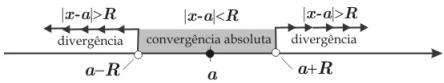
\includegraphics[width=0.7\textwidth]{intervalos-convergencia.jpg}
\caption{Intervalos de Convergência com centro \(a=b\)}
\label{fig:3-1B}
\end{figure}


\begin{theoc}{}{teorem-3-1}
As séries de potências \(\sum a_{n}(x-b)^{n}\) satisfazen apenas uma das seguintes condições
\begin{tasks}[label=(\alph*),item-indent=1.5cm, label-width=2em,ref=(\alph*)](1)
  \task a série converge apenas quando \(x=b\);
  \task a série converge absolutamente para qualquer valor que se atribua a \(x\);
  \task existe um número real \(R > 0\), denominado raio de convergência, tal que a série converge 
  absolutamente \(|x-b|<R\) e diverge quando \(|x-b| > R\).
\end{tasks}
\end{theoc}

Com relação ao raio de convergência \(R\) estabelecido no Teorema~\ref{thm:teorem-3-1}, nos casos em que 
ocorrer a condição (a) diremos que o raio de convergência é \(R = 0\) e quando a série for convergente em 
qualquer valor de \(x\) diremos que o raio de convergência da série é \(R = \infty\). Assim, toda série de 
potências tem um raio de convergência que pode ser zero, um número real positivo ou \(\infty\). 

Uma maneira prática de calcular o raio de convergência de uma série de potências é estabelecida no 
seguinte critério.

\begin{theoc}{Critério da Razão}{}
Se o limite do quociente
\begin{equation*}
l=\lim_{n\, \to\, \infty}\left|\dfrac{a_{n+1}}{a_{n}}\right| \neq 0 
\end{equation*} 
então o raio de convergência \(R\) da serie de potências 
\begin{equation*}
  \sum_{n\, =\, 0}^{\infty}a_{n}(x-b)^{kn+p} \quad\text{é}\quad  R=\left(\dfrac{1}{l}\right)^{1/k}, \quad k >0
\end{equation*}
\begin{tasks}[label=(\alph*),item-indent=3em,label-width=2em,ref=(\alph*)](2)
  \task  Se o valor de \(l=0\), então \(R=\infty\)
  \task Se o valor de \(l = \infty\), então \(R = 0\)
\end{tasks}
\end{theoc}

\begin{prvc}{}{}
Representando por \(a_{n}\) o termo geral da série, então \(z_{n}(x)=a_{n}(x-b)^{kn+p}\) e temos,
\begin{equation*}
L(x)=\lim_{n\, \to\, \infty}\left| \dfrac{z_{n+1}(x)}{z_{n}(x)}\right|=
\lim_{n\, \to \, \infty}\left|\dfrac{a_{n+1}(x-b)^{kn+k+p}}{a_{n}(x-b)^{kn+p}}\right| 
=|x-b|^{k}\lim_{n\, \to \, \infty}\left|\dfrac{a_{n+1}}{a_{n}}\right|=|x-b|^{k} \cdot l 
\end{equation*}
e usando o critério da razão deduzimos que,
\begin{tasks}[label=(\alph*),item-indent=3em,label-width=2em,ref=(\alph*)](1)
\task se \(l=0\), então \(L=0\) e a série converge absolutamente em
qualquer valor que se atribua a \(x\) e, neste caso, \(R= \infty\); 
\task se \(l=\infty\), então a única possibilidade  de se ter \(L < 1\) ocorre quando \(x=b\) e, 
neste caso, \(R=0\); 
\task finalmente, se \(0 < l < \infty\), então a série converge absolutamente se 
\(|x-b|^{k} \cdot l < 1\), isto é, \(|x-b| < (1/l)^{1/k}\) e diverge se 
\(|x-b|^{k} \cdot l > 1\), isto é, \(|x-b| \cdot  l > (1/l)^{1/k}\). 
Neste caso deduzimos que \(R = (1/l)^{1/k}\). \hfill \(\square\)
\end{tasks}
\end{prvc}

\begin{exer} Consideremos a série de potências,
\begin{equation*}
\sum_{n\geq 0}a_nx^n \quad  \text{onde} \quad a_n=\dfrac{1}{n!}. 
\end{equation*}
  
  Mostre que é absolutamente convergente em $\mathbb{R}$.
\end{exer}

\solo Aplicando o critério da razão, temos
\[
\left|\frac{[1/(n+1)!]x^{n+1}}{(1/n!)x^{n}}\right|=\frac{|x|}{n+1}
\]
e, para qualquer $x$, esta razão tende para zero quando $n$ vai ao
infinito. Portanto, a série dada converge absolutamente em
$-\infty < x < \infty$ e uniformemente em todo intervalo finito fechado
$-R_1\leq x \leq R_1$.\hfill \(\lozenge\)

\begin{exer}
Se para $\sum a_nx^n$ existe o limite
\begin{equation*}
  L = \lim_{n\to\infty}\left|\frac{a_{n+1}}{a_n}\right|
\end{equation*}
então o raio de convergência da série é $R = 1/L$.
\end{exer}

\solo Neste caso obtemos a razão
 \begin{equation*}
  \left| \frac{a_{n+1}x^{n+1}}{a_nx^n} \right|=\left| \frac{a_{n+1}}{a_n}\right||x|
 \end{equation*}
que converge para $L|x|$ quando $n$ vai ao infinito. Portanto, a
série converge se $L|x| <1$  e diverge se $L|x|>1$, isto e, converge se $|x| <R$ e 
diverge se $|x|>R$.\hfill \(\lozenge\)

\begin{exer}
Encontrar o intervalo de convergência das seguintes séries,
\begin{tasks}[label=(\alph*),label-width=4ex,ref=(\alph*)](3)
\task \(\dst \sum_{n\geq 0}(-2)^n\left(\frac{n+2}{n+1}\right)x^n\)
\task \(\dst \sum_{n\geq 0}\frac{(-1)^{n+1}\;x^{2n-1}}{(2n-1)!}\)
\task \(\dst \sum_{n\geq 0}\frac{(-1)^{n}\;x^n}{(2n-1)\,3^{2n-1}}\)
\end{tasks}
\end{exer}

\solo Resolveremos o primeiro, pelo critério da razão temos que o
quociente,
\begin{equation*}
    \left|(-2)^{n+1}\left(\frac{n+3}{n+2}\right)x^{n+1}\cdot\frac{1}{(-2)^n}
    \left(\frac{n+1}{n+2}\right)\frac{1}{x^n}
    \right|=2\frac{(n+3)(n+1)}{(n+2)^2}|x|,
\end{equation*}
converge para $2|x|$ quando $n$ vai ao infinito. Pelo critério
citado a série será absolutamente convergente quando $|x|<1/2$ e
diverge para $|x|>1/2$. Os casos onde $|x|=\pm 1/2$ são estudados
por separado.

Quando $x=\pm 1/2$ temos as séries numéricas:
\begin{align*}
    \sum_{n\ge 0}(-1)^n\left(\frac{n+2}{n+1}\right)\qquad \text{ e
    }\qquad \sum_{n\ge 0}\left(\frac{n+2}{n+1}\right)
\end{align*}
respectivamente, e pelo critério do limite do n-ésimo termo (critério da divergência) ambas são divergentes. Em conclusão a
série dada converge no intervalo $|x|<1/2$. Para as outras séries fazemos o mesmo estudo.\hfill \(\lozenge\)


Os teoremas concernentes à derivação e à integração de séries de potências são obtidos facilmente 
a partir do Teorema~\ref{thm:1117-26}.

\begin{theoc}{}{1117-27} Se a série de potências
\[
 F(x)=\sum_{n\geq 0}a_n\,x^n
\]
tem raio de convergência $R$, então $\dst{\int_c^dF(x)dx}$ existe para $-R < c < d < R$ \quad e
\begin{equation}\label{1117-12}
\int_c^dF(x)dx=\sum_{n\geq 0}\int_c^d a_nx^ndx=\sum_{n\geq
0}a_n\left(\frac{d^{n+1}-c^{n+1}}{n+1}\right).
\end{equation}
\end{theoc}

\prova Conforme o Teorema~\ref{thm:1117-26}, a série converge
uniformemente no intervalo $c< x <d$. Portanto, \eqref{1117-12}
decorre dos resultados gerais relativos à integração de séries
uniformemente convergentes.\qed

\begin{theoc}{}{1117-28}
Se a série de potências $F(x)=\sum_{}a_nx^{n}$ tem raio
de convergência $R$, então $F'(x)$ existe em $-R< x <R$  e sua derivada é,
\begin{equation}\label{1117-13}
 F'(x)= \sum_{n\,=\, 1}^{\infty}n\,a_n\,x^{n-1}.
 \end{equation}
\end{theoc}

\prova De acordo com o teorema geral sobre derivação de séries,
precisamos apenas mostrar que a série derivada \eqref{1117-13}
converge uniformemente em todo intervalo $- R_1 < x < R_1$, para
os quais $R_1 < R$. Para este fim, escolhamos $x_1$, tal que $R_1
< x_1< R$. Então, $\sum_{}a_n\,x^n_{1}$ converge
absolutamente, e, consequentemente, existe um número $M$, tal que
$|a_n\,x^n_1|<M$ para todo $n$. Então, para $|x_1| < R_1$, temos
\begin{align*}
   |na_nx^{n-1}|&=n|a_n||x|^{n-1}
   \leq n|a_n|R_1^{n-1}  \\[2ex]
  &\leq n\frac{M}{|x_1|^n}R_1^{n-1}=n\frac{M}{|x_1|}\left|\frac{R_1}{x_1}\right|^{n-1}
\end{align*}

No entanto, a série
\[
\sum_{n\geq 1}n\frac{M}{|x_1|}\left|\frac{R_1}{x_1}\right|^{n-1},
\]
converge pelo teste da razão, e a convergência uniforme de
\eqref{1117-13} resulta agora do critério M-Weierstrass. \qed

\begin{exer}
Encontre  uma  série de Maclaurin que defina a função dada, e determine o raio de convergência.
\begin{align*}
\rm{(a)}&\quad \ln(1+x)\quad &\rm{(b)}&\quad \frac{\ln(1+x)}{1+x^2} \quad &\rm{(c)}&\quad \int_o^x e^{-t^2}\,dt
\end{align*}
\end{exer}

\solo Resolvemos a primeira questão (a), lembrando a série geométrica
e integrando ambos lados,
\begin{align*}
    \frac{1}{1+t}&=\sum_{n\ge 0}(-1)^nt^n,\qquad |t|<1\\[2ex]
    \intertext{ integrando de \(0\) até \(x\), \(-1 <x <1\) }
    \int_{0}^{x}\dfrac{dt}{1+t}=\ln(1+x)=&\sum_{n\ge 1}\int_0^x(-1)^nt^n\,dt=\sum_{n\ge
    0}(-1)^n\frac{x^{n+1}}{n+1},\qquad |x|<1.
\end{align*}
onde seu raio de convergência é $R=1$. Para o segundo exercício (b)
tomamos a expressão acima obtida e multiplicamos pela série
geométrica,
\begin{align*}
\ln(1+x)=&\sum_{n\ge
    1}(-1)^n\frac{x^{n+1}}{n+1},\qquad |x|<1\\[2ex]
    \intertext{ por outro lado }
\frac{1}{1+x^2}&=\sum_{n\ge 0}(-1)^nx^{2n},\qquad |x|<1
\end{align*}

Multiplicando termo a termo obtemos,
\begin{equation*}
    \frac{\ln(1+x)}{1+x^2}=\sum_{k\ge
    0}c_k\,x^k=x-\frac{x^2}{2}-\frac{2}{3}x^3+\frac{1}{4}x^4-\frac{13}{15}x^5+\cdots,\quad
    |x|<1
\end{equation*}
onde $\dst{c_k=\sum_{l+m=k}a_lb_m}$ e o raio de convergência é
$R=1$. 

Finalmente no último exercício  (c) utilizamos a expressão da
série exponencial 
\begin{align*}
    e^{-x}=\sum_{n\ge 0}(-1)^n\frac{x^n}{n!},\qquad x\in
    \mathbb{R}\\
    \intertext{ substituindo o argumento }
e^{-t^2}=\sum_{n\ge 0}(-1)^n\frac{t^{2n}}{n!},\qquad x\in
\mathbb{R}.
\end{align*}

A seguir e integramos termo a termo, de \(0\) até \(x\), com \(x \in \mathbb{R}\)
\begin{align*}
    \int_0^xe^{-t^2}dt &= \sum_{n\, =\, 0}^{\infty}\dfrac{(-1)^{n}}{n!(2n+1)}x^{2n+1}\\[2ex]
    & =x-\frac{x^3}{3}+\frac{x^5}{2!5}+\frac{x^7}{3!7}+
    \cdots+\frac{(-1)^n}{n!}\frac{x^{2n+1}}{(2n+1)}+\cdots\quad
    x\in \mathbb{R}
\end{align*}
logo o raio de convergência é $R=\infty$. \hfill \(\lozenge\)

Informalmente, os dois teoremas precedentes afirmam que se pode integrar ou derivar uma série de potências, \textit{termo a termo}, sem afetar o raio de convergência. A convergência em $|x| = R$ pode ser desfeita por derivação ou adquirida por integração, mas isto só pode ser comprovado, examinando-se cada série, individualmente. \hfill \(\lozenge\)

\begin{exer}
Consideremos as seguintes séries de funções
\begin{tasks}[label=(\alph*),label-width=4ex,item-indent=2cm,ref=(\alph*)](2)
\task \(\dst{\sum_{n\,=\, 0}^{\infty}x^n=1+x+x^2+\cdots}\)
\task \(\dst{\sum_{n\, =\, 0}^{\infty}\dfrac{x^{n+1}}{n+1}=x+\dfrac{x^2}{2}+\cdots}\)
\task \(\dst{\sum_{n\, =\, 0}^{\infty}\dfrac{x^{n+2}}{(n+1)(n+2)}=
\dfrac{x^2}{2}+\dfrac{x^3}{2\cdot3}+\cdots}\)
\end{tasks}

Examine cada uma e responda sobre sua convergência ou divergência.
\end{exer}

\solo Cada uma destas séries tem raio de convergência $R = 1$,
porque (a) é uma série geométrica, (b) e (c) se obtém de (a) por
integração. Vemos, porém, que a série (a) diverge tanto em $x = 1$
como em $x=-1$, a série (b) converge em $x=-1$, mas diverge em $x
= 1$, e a série (c) converge nos dois extremos. \hfill \(\lozenge\)


Existem muitas implicações interessantes do teorema referente à  derivação de séries de 
potências. Se $\sum a_n\,x^n$ converge em $- R < x < R$, então ela representa 
(converge para) uma função contínua,
\begin{equation*}
  F(x) = \sum_{n\, =\, 0}^{\infty}a_n\,x^n.
\end{equation*}

E mais, $F'(x)$, \(F''(x)\ldots\) existem neste intervalo e
\begin{align*}
F'(x) &= \sum_{n\,=\,1}^{\infty}n\,a_{n}\,x^{n-1},\quad  -R < x < R,\\[2ex]
F''(x) &= \sum_{n\,=\,2}^{\infty}n\,(n-1)\,a_{n}\,x^{n-2},\quad  -R < x < R,\\[2ex]
F'''(x) &= \sum_{n\,=\,3}^{\infty}n\,(n-1)(n-2)\,a_{n}\,x^{n-3},\quad  -R < x < R,
\end{align*}

Repetindo o processo de derivação até a ordem \(n\), obtemos
\begin{equation*}
F^{(n)}(x) =\sum_{k\,=\, n}^{\infty} k(k - 1)(k - 2) ... (k - n + 1)a_k\,x^{k-n},\quad 
-R < x < R.
\end{equation*}
para $n\ge 1$  e, por conseguinte, $F^{(n)}(0)=n!\,a_n$. Com isto
demonstramos o

\begin{theoc}{}{1117-29}
Se uma função $F$ pode ser representada por uma série de potências
 $\sum_{}a_n\,x^{n}$ no intervalo $-R < x < R$, então $F$ tem
derivadas de todas as ordens em $- R < x < R$ e os coeficientes da
série são unívocamente determinados pela relação
\begin{equation*}
a_{n} = \dfrac{1}{n!}F^{(n)}(0),\quad  a_{0} = F(0).
\end{equation*}
\end{theoc}

O Teorema~\ref{thm:1117-29} estabelece a \textit{unicidade} do
desenvolvimento em série de potências de uma função $F$ num dado
intervalo $- R < x < R$. A existência de tal série é problema mais
difícil, e o estudaremos na próxima seção. Observamos,
naturalmente, que, para que uma função $F$ tenha uma representação
em série de potências, é necessário que $F$ tenha derivadas de
todas as ordens. Esta condição exclui, por exemplo, a função $\ln
|x|$ que não seja definida em $x = 0$ e a função $x^{8}/3$ para a
qual a derivada de terceira ordem deixe de existir em $x = 0$.
Infelizmente, a existência de uma infinidade de derivadas, de $F$
em $- R < x < R$ não é o suficiente para garantir a
representabilidade de $F$ por uma série de potências.

\begin{exer}
Seja  função $f$ definida por
\begin{equation*}
  f(x)=
    \begin{cases}
      e^{-1/x^2} & \quad  \text{ se }\quad x\neq 0 \\[2ex]
      \phantom{xx}0 & \quad \text{ se } \quad x=0.
    \end{cases}
\end{equation*}

Mostre que não converge para uma função não nula.
\end{exer}

\solo Vejamos que a função dada possui  derivadas de todas as
ordens em  $\mathbb{R}$. Todavia, 
\begin{equation*}
  f^{(n)}(0) = 0  \quad \text{para todo}\quad  n,
\end{equation*}
e a série de potências  
\begin{equation*}
\sum_{n\, =\, 0}^{\infty}\,\dfrac{f^{(n)}(0)}{n!}\,x^{n}
\end{equation*}
converge em $\mathbb{R}$ para a função que seja identicamente nula, e não
para $f$.\hfill \(\lozenge\)


Encerramos esta seção com vários resultados aritméticos
concernentes a séries de potências.

\begin{teo}\label{1117-30} Se a seguintes funções
\begin{equation*}
f(x) =\sum_{n\geq 0}a_nx^n \qquad \text{ e } \qquad g(x)=\sum_{n\geq 0}b_nx^n
\end{equation*}
em $- R < x < R$, então, para quaisquer constantes $\al$, $\be$ a
série $\sum_{}(\al a_n+\be b_n)x^n$ tem raio de
convergência pelo menos $R$ e representa a função $\al f(x) + \be
g(x)$ em $- R < x < R$.
\end{teo}

\prova A demonstração do teorema é uma consequência imediata do
Teorema de sequências convergentes.\hfill $\Box$

\begin{theoc}{}{1117-31} Se as funções
\begin{equation*}
  f(x) =\sum_{n\geq 0}a_nx^n \qquad \text{ e } \qquad g(x)=
  \sum_{n\geq 0}b_nx^n \quad \text{em}\quad - R < x < R,
\end{equation*}
então a série $\sum_{}c_n\,x^{n}$, onde
\begin{equation}\label{1117-14}
c_n =\sum_{k = 0}^{n}a_{k}b_{n-k}=a_{0}\,b_n+a_{1}\,b_{n-1}+\cdots+a_{n}b_{0},
\end{equation}
converge para o produto $fg$ em $- R < x < R$.
\end{theoc}

O leitor notará que os coeficientes \eqref{1117-14} são exatamente
aqueles que se obtém mediante a ``multiplicação formal'', das
séries dadas, considerando-as como polinômios.

\begin{exer}
Encontrar a expansão em séries de potências das funções
\begin{align*}
\rm{(a)}&\quad \quad e^{x^2-1}\quad &\rm{(b)}&\quad \frac{1-x}{1+2x+x^2}
\end{align*}
\end{exer}

\solo Resolvendo o primeiro item (a) por médio de
\begin{equation*}
    e^{x^2-1}=e^{x^2}e^{-1}=e^{-1}\sum_{n\ge
    0}\frac{x^{2n}}{n!},\qquad x\in \mathbb{R}
\end{equation*}
onde o raio de convergência é $R=\infty$. O segundo item (b) do exercício
exige alguma modificação antes de encontrar a série,
\begin{equation*}
\dfrac{1-x}{1+2x+x^2}=\dfrac{(1-x)(1+x)}{(1+2x+x^2)(1+x)}=\dfrac{1-x^2}{(1+x)^3}=
(1-x^2)(1+x)^{-3}.
\end{equation*}

Utilizando a série binômial, uma expansão em séries de potências, com \(\alpha\in \mathbb{R}\),
\begin{equation*}
  (1+x)^{\al}=1+\al x+\frac{\al(\al-1)}{2!}x^2+\cdots+\frac{\al(\al-1)(\al-2)\cdots(\al-n+1)}{n!}x^n+\cdots
\end{equation*}
válida no intervalo $|x|<1$. Usando \(\alpha=-3\) temos
\begin{align*}
\frac{1-x}{1+2x+x^2}&=(1-x^2)(1+x)^{-3} =(1-x^2)(1-3x+6x^{2}-10x^{3}+15x^{4}-84x^{5}+\cdots),\\[2ex]
&=1-3x+5x^{2}-16x^{3}+9x^{4}-74x^{5}+\cdots, \qquad |x|<1.
\end{align*}
com raio de convergência $R=1$.\hfill \(\lozenge\)

Como último comentário, observamos que, até agora, temos estudado série de potências 
$\sum_{}a_n\,x^{n}$ cujo intervalo de convergência se encontra centrado no ponto $x = 0$. Toda 
a discussão pode muito bem ser estendida a séries da forma $\sum_{}a_{n}(x-b)^{n}$. O intervalo 
de convergência destas séries é da forma $b - R < x < b + R$ (com ou sem os extremos) e se calcula o 
raio de convergência $R$ com as mesmas técnicas apresentadas anteriormente.

Em particular, se
\begin{equation*}
  f(x) =\sum_{n\,=\, 0}^{\infty} a_n(x - b)^n\quad \text{em}\quad b - R < x < b +R,
\end{equation*}
então $f$ possui uma infinidade de derivadas nesse intervalo e os coeficientes são 
\begin{equation*}
  a_{n} = \dfrac{1}{n!}\,f^{(n)}(b).
\end{equation*}

\begin{exer}
Encontrar as séries de potências para as funções dadas
\begin{tasks}[label=(\alph*),item-indent=1.5cm,label-width=4ex,ref=(\alph*)](2)
\task \(f(x)=\sen^2 x\quad  \text{em potências de} \quad  x.\) 
\task \(g(x)=\senh x\quad  \text{em potências de}  \quad  x.\)
\task \(h(x)=e^{x/2}\quad \text{em potências de}  \quad x-2.\)
\end{tasks}
\end{exer}

\solo Feito em sala de aula. \hfill \(\lozenge\)

%%%%%%
\section*{Exercícios Propostos}
%%%%%%%%%%%%%%
\begin{enumerate}[label=(\arabic*)]
\item Encontre um exemplo de uma  \seq\ $u_n\colon [0,1] \to
  \mathbb{R}$ que converge para zero pontualmente, por\'em a
  integral $\dst{\int_0^1u_n(x)\;dx}$ n\ao\ converge para zero.

\item Considere a \seq\ $u_n(x)=\dst{\frac{n x}{1+nx}},\quad 0\leq x\leq
  1$. Em que subintervalos existe a \conv\ da derivada? A
  func\ao\ limite \'e diferenci\'avel em $x=0$?

\item Verificar o valor de $\dst{\int_0^x e^t dt= e^x -1}$,
  usando $\dst{e^x=\sum_{n\geq1}\frac{x^n}{n!}}$.

\item Mostre que a \seq\ $\{u_n\}_{n\geq 1}$ definida por
  $$u_n(x)=n^3x^n(1-x),$$
converge pontualmente para $u=0$ no intervalo $[0,1]$ e mostre que
a \conv\ n\ao\ \'e uniforme.

\item Verificar que $\dst{\int_0^x\sen t dt=1-\cos x}$, utilizando
a seguinte rela\cao :
$$
\sen x = \sum_{n\geq 0}(-1)^n\frac{x^{2n+1}}{(2n+1)!}.
$$

\item Encontre o intervalo de converg\^encia das seguintes s\'eries,
\begin{tasks}[label=(\alph*),label-width=2em,ref=(\alph*)](2)
\task \(\dst\sum_{n\geq 0}\frac{x^n}{(n+1)} \)
\task \(\dst \sum_{n\geq 1}n!\, x^{n}\)
\task \(\dst \sum_{n\geq 1}(-1)^n\frac{x^n}{(2n-1)3^{2n-1}}\)
\task \(\dst \sum_{n\geq 1}(-1)^{n+1}\frac{(n+1)x}{n!}\)
\task \(\dst \sum_{n\geq 1}\dfrac{(x+2)^n}{(n+1)2^n}\)
\task \(\dst \sum_{n\geq 1}(-1)^{n+1}\dfrac{(n+1)x}{n!}\)
\task \(\dst \sum_{n\geq 1}(-1)^n\dfrac{x^n}{(2n-1)3^{2n-1}}\)
\task \(\dst \sum_{n\geq 1}(-1)^{n+1}\dfrac{(n+1)x}{n!}\)
\task \(\dst \sum_{n\geq 1}(-1)^n\dfrac{x^n}{(2n-1)3^{2n-1}}\)
\task \(\dst \sum_{n\geq 1}(-1)^{n+1}\dfrac{(n+1)x}{n!}\)
\end{tasks}

\item Mostre que se o raio da convergência da s\'erie
$\dst{\sum_{n\geq 1}u_n x^{n}}$ \'e igual a $r$, ent\ao\ o raio de \conv\ da \ser\ $\dst{\sum_{n\geq 1}u_n x^{2n}}$ \'e igual a
$\sqrt{r}$.

\item Mostre que se $\dst{\lim_{n\to \infty }\sqrt[n]{|u_n|}=L},\; (L\not= 0)$, ent\ao\ o raio de \conv\  da \ser\ $\dst{\sum_{n\geq 1}u_n x^{n}}$ \'e igual a $\dst{\frac{1}{L}}$.

\item Considere a fun\cao\ $f$ definida por uma \ser\ de pot\^encias, a seguir fa\ca\ o seguinte:

(a) Encontre o raio de \conv\ e o dom\ii nio de $f$; (b) Escreva a \ser\ que define a $f'$ e encontre seu raio de
\conv; (c) Encontre o dom\ii nio de $f'$.
\begin{tasks}[label=(\roman*),label-width=2em,ref=(\alph*)](2)
 \task \(f(x)=\dst\sum_{n\geq 1}(-1)^{n-1}\dfrac{x^n}{n} \)
 \task \(f(x)=\dst \sum_{n\geq 1}\dfrac{x^n}{\sqrt{n}}\)
 \task \(f(x)=\dst \sum_{n\geq 2}\dfrac{(x-2)^n}{\sqrt{n-1}}\)
 \task \(f(x)=\dst \sum_{n\geq 1}(-1)^{n-1}\dfrac{x^{2n-1}}{(2n-1)!}\)
 \task \(f(x)=\dst \sum_{n\geq 1}\dfrac{x^{2n-2}}{(2n-2)!}\)
 \task \(f(x)=\dst \sum_{n\geq 1}\dfrac{(x-1)^n}{n\,3^n}\)
\end{tasks}

\item Execute os seguintes passos;
\begin{enumerate}
\item Encontre uma \ser\ de pot\^encias representando a fun\cao\ $\dst{\frac{e^{x}-1}{x}}$.
\item Por diferencia\cao\ termo a termo da \ser\ de pot\^encias do
item anterior mostre que  a \ser\ $\dst{\sum_{n\geq
1}\frac{n}{(n+1)!}=1}$.
\end{enumerate}
\item Execute os seguintes passos;
\begin{enumerate}
\item Encontre uma \ser\ de pot\^encias representando a fun\cao\ $x^2 e^{-x}$.
\item Por diferencia\cao\ termo a termo da \ser\ de pot\^encias do
item anterior mostre que  a \ser\ $\dst{\sum_{n\geq
1}(-1)^{n+1}\frac{n+2}{n!}=4}$.
\end{enumerate}
\end{enumerate}

%%%%%%%%%%%%%
\section{Polinômios e Séries de Taylor}
%%%%%%%%%%%%%
Na seção anterior vimos que, se uma função $f$ puder ser desenvolvida em uma série de potências da seguinte forma
\begin{equation*}
  f(x) = \sum_{n\, =\, 0}^{\infty}a_n(x - b)^n
\end{equation*}
num intervalo $|x - b| < R$, então $f$ terá derivadas de todas as ordens, e
\begin{equation*}
  a_n= \frac{1}{n!}\,f^{(n)}(b),\qquad  n = 0, 1, 2, \ldots
\end{equation*}

Mas existem funções que não podem ser expandidas em séries de potências. Na verdade, as funções que
 podem ser representadas em séries de potências são as que possuem infinitas derivadas e que se 
 encontram bem próximas do seu \emph{polinômio de Taylor}.

\begin{defic}{Polinômio de Taylor}{}
Dada uma função $f$ real que possui derivadas até a ordem $n$ num intervalo contendo $b$, o polinômio de 
Taylor de $f$ de grau $n$ em torno de $x=b$ é o polinômio,
\begin{equation}\label{taita001}
P_n(x)=f(b)+\frac{f'(b)}{1!}(x-b)+\frac{f''(b)}{2!}(x-b)^2+\cdots+\frac{f^{(n)}(b)}{n!}(x-b)^n
\end{equation}
\end{defic}

Quando o centro $b=0$ obtemos a partir da equação \eqref{taita001} o polinômio de MacLaurin
\begin{equation}\label{taita002}
P_n(x)=f(0)+\frac{f'(0)}{1!}x+\frac{f''(0)}{2!}x^2+\cdots+\frac{f^{(n)}(0)}{n!}x^{n}
\end{equation}

\begin{exer}
Determinar o polinomio de Maclaurin e o resto da expansão da função real \(f\) dada por  \(f(x)=\exp(x)\).
\end{exer}

\solo
Na situação de ter a função $f(x)=\exp(x)$, o correspondente polinômio de Maclaurin esta dado por
\begin{equation}\label{taita003}
P_n(x)=1+\dfrac{1}{1!}x+\dfrac{1}{2!}x^2+\cdots+\dfrac{1}{n!}x^{n}=s_{n}(x)
\end{equation}
e coincide com a $n$-ésima reduzida ou soma parcial \(s_{n}(x)\), da série $\dst{\sum x^n/n!}$ que representa a 
função real $\exp(x)$. Para essa função exponencial, temos o fato
\begin{equation*}
  \lim_{n \to \infty}\frac{b^n}{n!} = 0 \quad \text{ para todo} \quad b \in \mathbb{R}
\end{equation*}

Deduzimos que para o número $\xi$ com $0<\xi <x$ o limite
\begin{equation}\label{taita004}
\lim_{n \to \infty} \frac{f^{(n+1)}(\xi)}{(n+1)!}(x-b)^{n+1}=e^{\xi}\lim_{n \to \infty} 
\dfrac{1}{(n+1)!}(x-b)^{n+1}=0.
\end{equation}

O termo dado pela expressão,
\begin{equation*}
  R_n(x,\;\xi)=\frac{f^{(n+1)}(\xi)}{(n+1)!}(x-b)^{n+1}
\end{equation*}
que aparece no limite \eqref{taita004} é chamado de \emph{resto da aproximação} da função $f$ pelo 
seu polinômio de Taylor. O resultado a seguir, conhecido como \emph{Fórmula de Taylor com Resto}, afirma
 que uma função derivável de classe $C^{n+1}$ em torno de um ponto tem a propriedade \eqref{taita004} se, 
 e somente se, ela puder ser aproximada pelo seu polinômio de Taylor. \hfill \(\lozenge\)


Consideremos agora a questão da \textit{existência} de uma tal representação em série de potências para 
uma dada função $f$.
\begin{theoc}{Fórmula de Taylor com Resto I}{taita005}
Seja $f$ uma função real de classe $C^{n+1}$ num intervalo que contém $b$. Dado qualquer $x$ nesse 
intervalo, existe um número $\xi$ entre $b$ e $x$ tal que
\begin{equation}\label{taita006}
  f(x)=P_n(x)+R_n(x,\;\xi)
\end{equation}
onde $P_n(x)$ ó polinômio de Taylor de $f$. Além disso para sequência $\{P_n(x)\}$, temos
\begin{equation}\label{taita007}
  P_n(x)\to f(x) \quad \text{ se e somente se }\quad \lim_{n \to \infty} 
  \dfrac{f^{(n+1)}(\xi)}{(n+1)!}(x-b)^{n+1}=0
\end{equation}
\end{theoc}

\prova Feito em sala de aula. \qed

Denotando pelo símbolo $\{s_n(x)\}$ a sequência de somas parciais da série,
\begin{equation*}
  \sum_{n \,=\, 0}^{\infty} \frac{f^{(n)}(b)}{n!}(x-b)^{n}\quad \text{ onde a função $f$ é de classe } 
  \quad C^{\infty}(I),\; b\in I
\end{equation*}
e assim deduzimos,
\begin{equation*}
  \lim_{n \to \infty}s_n(x)=\lim_{n \to \infty}P_n(x)=\lim_{n \to \infty}[f(x)-R_n(x)]=
  f(x)-\lim_{n \to \infty}R_n(x)=f(x)
\end{equation*}
isto quer dizer que a série converge para $f(x)$ em cada $x$ do intervalo de convergência. Assim sendo, temos
\begin{equation}\label{taita008}
f(x)=\sum_{n \, =\, 0}^{\infty}\dfrac{f^{(n)}(b)}{n!}(x-b)^{n}
\end{equation}

A série de potências \eqref{taita008}  é chamada de \emph{Série de Taylor} de $f$ em torno de $x=b$. Quando 
$b=0$, a série correspondente é chamada \emph{Série de Maclaurin} de $f$.

\begin{exer}
Ilustre o Teorema~\ref{thm:taita005} (Fórmula de Taylor com Resto) anterior considerando a função $f(x)=\exp(x)$
\end{exer}

\solo As derivadas da função $f$ no ponto $x=0$ é dada pela fórmula $f^{(k)}(0)=1$. Portanto o polinômio de Taylor e seu resto
\begin{equation*}
P_n(x)=1+x+\frac{1}{2!}x^2+\cdots+\frac{1}{n!}x^n, \quad  R_n(x,\;\xi)=\frac{e^{\xi}}{(n+1)!}(x-b)^{n+1}
\end{equation*}
para algum número $\xi$ entre $0$ e $x$. De maneira que
\begin{equation*}
  \exp(x)=1+x+\frac{1}{2!}x^2+\cdots+\frac{1}{n!}x^n+\frac{e^{\xi}}{(n+1)!}(x-b)^{n+1}
\end{equation*}

Aplicando limite quando $n$ vai ao infinito na seguinte diferença,
\begin{equation*}
  \exp(x)-\left(1+x+\dfrac{1}{2!}x^2+\cdots+\dfrac{1}{n!}x^n\right)=\dfrac{e^{\xi}}{(n+1)!}(x-b)^{n+1}
\end{equation*}
para obter,
\begin{equation*}
  \lim_{n\to \infty}[\exp(x)-P_n(x)]=0\quad \text{implica} \quad \lim_{n\to \infty}P_n(x)=\exp(x)
\end{equation*}


\begin{exer}
Ilustre o Teorema~\ref{thm:taita005} (Fórmula de Taylor com Resto) anterior considerando a função $f(x)=\sen(x)$.
\end{exer}

\solo Para a função $f(x)=\sen x$ temos as suas derivadas avaliadas no ponto $x=0$
\begin{align*}
 f(0)=0 && f'(0)=1 && f''(0)=0 && f'''(0)=-1 && f^{(iv)}(0)=0 &&\cdots
\end{align*}

Além disso o comportamento da derivada de ordem $n+1$ no ponto $\xi$ é,
\begin{equation*}
  f^{(n+1)}(\xi)=\left\{
                   \begin{array}{ll}
                   \pm \sen \xi & \quad \hbox{ se n for par }  \\[2ex]
                     \pm \cos \xi & \quad \hbox{ se n for ímpar }
                   \end{array}
                 \right.
\end{equation*}

Assim temos,
\begin{equation*}
  \sen x=x-\dfrac{x^3}{3!}+\dfrac{x^5}{5!}+\cdots+(-1)^n\dfrac{x^{2n+1}}{(2n+1)!}
  +\dfrac{f^{(n+1)}(\xi)}{(n+1)!}(x-\xi)^{n+1}
\end{equation*}

Aplicando limite a diferença em valor absoluto, quando $n$ vai ao infinito
\begin{equation*}
\left|\sen x -\left(x-\dfrac{x^3}{3!}+\dfrac{x^5}{5!}+\cdots+(-1)^n\dfrac{x^{2n+1}}{(2n+1)!}\right)\right|=
\left|\dfrac{f^{(n+1)}(\xi)}{(n+1)!}(x-\xi)^{n+1}\right|
\end{equation*}

Portanto o resto,
\begin{equation*}
R_n(x,\; \xi)=\left|\dfrac{f^{(n+1)}(\xi)}{(n+1)!}(x-\xi)^{n+1}\right|\leq 
\dfrac{|x-\xi|^{n+1}}{(n+1)!} \to 0
\end{equation*}
quando $n$ vai ao infinito.  Verificando que a série de Maclaurin da função $f(x)=\sen x$. Ou seja,
\begin{equation*}
  \lim_{n\to \infty}\left|\sen x -\sum_{k\,=\,0}^{n}(-1)^k\frac{x^{2k+1}}{(2k+1)!}\right|=0\quad 
  \text{ implica }\quad
  \sen x=\lim_{n\, \to\, \infty}\sum_{k\,=\, 0}^{n}(-1)^k\frac{x^{2k+1}}{(2k+1)!}
\end{equation*}
 com isto, fica concluído o exercício. \hfill \(\lozenge\)

 \begin{exer}
Encontre as séries das funções reais dadas por,
\begin{tasks}[label=(\alph*),item-indent=3em,label-width=4ex,ref=(\alph*)](3)
  \task \(f(x)=\sen^{2}(x)\)
  \task \(g(x)=\cos^{2}(x)\)
  \task \(h(x)=x^{2}\sen(x)\)
\end{tasks}
 \end{exer}

 \solo
Combinando as séries de \(sen(x)\) e \(cos(x)\) e usando alguns artifícios simples encontramos séries que
representam as funções dos itens deste exercicio, no item (a) é resolvido usando a relação
\begin{equation*}
  \sen^{2}(x)=\dfrac{1}{2}\left[1-\cos(2x)\right]
\end{equation*}
que lineariza a função \(\sen^2(x)\) juntamente com a série de potencias que representa \(cos(x)\), com o 
argumento \(2x\) no lugar de \(x\). 

Para item (b) usamos a linearização da função cosseno dada por,
\begin{equation*}
\cos^{2}(x)=\dfrac{1}{2}\left[1+\cos(2x)\right]
\end{equation*} 

Finalmente para o item (c) a série de potencias da função \(h\) 
é obtida simplesmente multiplicando a série de \(sen(x)\) por \(x^{2}\). Neste caso, obtemos,
\begin{equation*}
h(x)=x^{2}\,\sen(x)=x^{2}\sum_{n\, =\, 0}^{\infty}\dfrac{(-1)^{n}}{(2n+1)!}x^{2n+1}=
\sum_{n\, =\, 0}^{\infty}\dfrac{(-1)^{n}}{(2n+1)!}x^{2n+3}
\end{equation*}
e isso conclui o exercício. \hfill \(\lozenge\)

\begin{exer}
A partir da série geométrica no intevalo \(|x|<1\) obtenha a representação em séries de poteêcias
da função 
\begin{tasks}[label=(\alph*),item-indent=3em,label-width=4ex,ref=(\alph*)](2)
\task \(w(x)=\dfrac{1}{(1-x)^{2}}\) 
\task \(\theta(x)=\dfrac{x}{(1-x)^{2}}\)   
\end{tasks}
\end{exer}

\solo
Considerando a série geométrica, para o item (a),
\begin{equation*}
  \dfrac{1}{1-x}=\sum_{n\,=\,0}^{\infty}x^{n} \quad |x| < 1.
\end{equation*}

Derivando termo a termo num subintervalo fechado de \(|x|<1\),
\begin{equation*}
\dfrac{d}{dx}\left( \dfrac{1}{1-x}\right)=\dfrac{d}{dx}\left(\sum_{n\,=\,0}^{\infty}x^{n}\right)
=\sum_{n\,=\,0}^{\infty}\dfrac{d}{dx}\left(x^{n}\right)=\sum_{n\,=\,0}^{\infty}n\,x^{n-1}
\end{equation*}
e assim obtemos a representação,
\begin{equation*}
w(x)=\dfrac{1}{(1-x)^{2}}= \sum_{n\,=\,0}^{\infty}n\,x^{n-1}, \quad |x|<1.
\end{equation*} 

Finalmente o item (b) é obtido multiplicando a última série por \(x\), 
\begin{equation*}
\theta(x)=\dfrac{x}{(1-x)^{2}}= \sum_{n\,=\,0}^{\infty}n\,x^{n}, \quad |x|<1.
\end{equation*}
e assim concluimos o exercício. \hfill \(\lozenge\)


\begin{theoc}{Fórmula de Taylor com Resto II}{1118-32}
Suponhamos que $f$ e suas $n + 1$ derivadas sejam definidas e contínuas no intervalo $I$ definido por $|x - a| < R$. Então, para todo $x$ em $I$, temos
\begin{equation}\label{1118-15}
  f(x)=\sum_{k\, =\, 0}^{n}\dfrac{f^{(k)}(b)}{k!}(x-b)^k+R_n(x),  
\end{equation}
onde o resto é dado por
\begin{equation}\label{1118-16}
R_n(x)=\dfrac{1}{n!}\int_{b}^x(x-t)^n\,f^{(n+1)}(t)\,dt.
\end{equation} 
\end{theoc}

\prova Comecemos com a fórmula
\begin{equation*}
  f(x) - f(a)=\int_a^xf'(t) dt.
\end{equation*}

Transpondo $f(b)$ para o segundo membro desta equação e integrando
por partes [com $u = f'(t),\quad dv = dt$] obtemos
\begin{equation*}
  f(x) = f(a) + [f'(t)(t - x)]^x_a - \int_a^x(t-x)f^{(2)}(t)\, dt
\end{equation*}
ou
\begin{equation*}
  f(x) = f(a) + f'(a)(x - a) +\int_a^x(t-x)f^{(2)}(t) dt
\end{equation*}
onde a fórmula de integração por partes foi escrita na forma
$\dst{\int u dv = u(v + c) - \int(v + c)du}$ em que $c$ e é uma
constante arbitrária.

Integremos novamente por partes, fazendo $u=f^{(2)}(t)$ e $dv =(x
- t) dt$, para obter
\begin{align*}
  f(x)&=f(b)+ f'(b)(x - a)+\left[ f^{(2)}(t)\cdot\frac{-(x-t)^2}{2!} \right]_a^x
  -\int_b^x\frac{-(x-t)^2}{2!}f^{(3)}(t)\, dt  \\[2ex]
   & =f(b)+f'(b)(x-b)+\dfrac{f^{(2)}(b)}{2!}(x-b)^2+
   \int_a^x\frac{(x-t)^2}{2!}f^{(3)}(t)\, dt.
\end{align*}

Continuando a integrar por partes (demonstração por indução
matemática), chegaremos às fórmulas desejadas, depois de $n$
integrações. (Observemos que se podem efetuar as integrações,
desde que os integrandos sejam contínuos.) \qed


\begin{exer} A função $f(x) = x^{8/3}$ tem derivadas contínuas até a ordem
dois no intervalo $-\infty < x < \infty$.
\end{exer}

\solo Portanto, quando $b = 8$, a fórmula de Taylor fornece
\begin{align*}
f(x) = x^{8/3}&=f(8)+f'(8)(x-8)+\int_8^x(x-t)f^{(2)}(t)\, dt \\[2ex]
    &=256+\dfrac{256}{3}(x-8)+\dfrac{40}{9}\int_8^x(x-t)t^{2/3}\, dt
\end{align*}

Se $f$ tem derivadas de todas as ordens no ponto \(b\) é 
natural considerar a série de \textit{Taylor infinita}
\begin{equation}\label{1118-17}
\sum_{n\, =\, 0}^{\infty}\dfrac{f^{(n)}(b)}{n!}(x-b)^{n}
\end{equation}
e perguntar se esta série converge para $f$ num intervalo $|x - b|
< R$. Aplicando o Teorema~\ref{thm:1118-32}, podemos afirmar que
\eqref{1118-17} converge para $f$ quando $|x - b| < R$ se, e
somenente se,
\begin{equation*}
  \lim_{n\to\infty} R_n(x) = 0,
\end{equation*}
para todo $x$ do intervalo. Logo, para resolver esta questão, basta determinar o comportamento 
de $R_n(x)$ quando $n$ vai ao infinito.
\hfill \(\lozenge\)

Para isto, o seguinte resultado é particularmente útil.

\begin{theoc}{}{1118-33}
Se $f$ satisfizer às condições do Teorema~\ref{thm:1118-32} e se
existir um número $M$ positivo, tal que $|f^{(n+1)}(x)|\leq M$ para $|x-b| < R$, então
\begin{equation}\label{1118-18}
|R_n(x)|\leq M \frac{|x - b|^{n+1} }{(n + 1 )!}
\end{equation}
\end{theoc}

\prova Suponhamos, primeiro, que $x\geq b$; então,
\begin{align*}
  |R_n(x)|=\left|\dfrac{1}{n!}\int_{b}^x(x-t)^nf^{(n+1)}(t)\, dt \right|
  =M\frac{(x-b)^{n+1}}{(n+1)!}
\end{align*}

Se, por outro lado, $x\leq b$, então
\begin{equation*}
  |R_n(x)|\leq \dfrac{M}{n!}\int^{b}_x(t-x)^n\,dt =M\,\dfrac{(b-x)^{n+1}}{(n+1)!}
\end{equation*}

A combinação destes resultados dá \eqref{1118-18}.\hfill $\square$

\begin{exer}\label{exem-2}
Se $f(x)= e^x$, a fórmula de Taylor fornecerá
\begin{equation*}
 e^x=1+ x + \frac{x^2}{2!}+\cdots+\dfrac{x^n}{n!} + R_n(x) \quad 
 \text{ com }\quad  R_n(x)=\dfrac{1}{n!}\int_0^x (x-t)^n\,e^t\, dt.
\end{equation*}

Como $|f^{n+1}(x)| =|e^x|\leq e^R$ no intervalo $|x| < R$, o Teorema~\ref{thm:1118-33} fornece
\begin{equation}\label{1118-19}
|R_n(x)|\leq e^R\frac{|x|^{n+1}}{(n+1)!},\qquad -R<x<R.
\end{equation}

Portanto, para qualquer $x$ desse intervalo,
\begin{equation*}
  \lim_{n\to\infty} R_n(x) = 0
\end{equation*}

Pois, para $x$ fixo, a série
\begin{equation*}
  \sum_{n\, =\, 0}^{\infty}\dfrac{|x|^{n+1}}{(n+1)!} < \infty
\end{equation*}
converge pelo teste da razão. Logo, seu termo geral tende para zero.

Como $R$ é arbitrário, segue-se que
\begin{equation}\label{1118-20}
e^x=\sum_{n, =\, 0 }^{\infty}\frac{x^n}{n!},\qquad x\in \mathbb{R}
\end{equation}
isto é, que o número $e$, é representado pela sua série de Taylor
na reta real.
\end{exer}

Pode-se aplicar a, estimativa \eqref{1118-19} também para efeito de cálculos. Por exemplo, encontremos o 
número de termos de \eqref{1118-20} necessários para calcular e com uma precisão de
sete casas decimais. Neste caso, temos (com $R = 1$)
\begin{align*}
e = e^1=\sum_{n\, =\, 0}^{\infty}\dfrac{1}{n!} +R_n(1) \quad \text{ e } 
\quad |R_n(1)|\leq \dfrac{e}{(n+1)!} < \dfrac{3}{(n+1)!}
\end{align*}


Podemos fazer esta última expressão tornar-se menor do que $10^{-7}$, escolhendo $n = 10$.

\begin{exer} 
Como as derivadas de $\sen x$ e $\cos x$ são limitadas,
cada uma, por $M = 1$ em $\mathbb{R}$, os restos de suas séries de
Taylor são limitados por $|x|^{}/(n + 1)!$. Portanto, a série de
Taylor converge, em cada caso, para a respectiva função no
intervalo $-\infty < x < \infty$.

O leitor pode, com facilidade, mostrar que as séries resultantes são
\begin{equation*}
\sen x =  x +\dfrac{x^3}{3!} +\dfrac{x^5}{5!}-\cdots,\quad 
\cos x =1-\dfrac{x^2}{2!}+\dfrac{x^4}{4!}-\cdots
\end{equation*}
\end{exer}

\begin{exer} Combinando o Exemplo~\ref{exem-2} com o Teorema~\ref{1117-30}, obtemos
\begin{align*}
\senh x = \dfrac{1}{2}(e^x - e^{-x}) = x +\dfrac{x^3}{3!} +\dfrac{x^5}{5!}+\cdots,\quad &&
\quad \cosh x = \dfrac{1}{2}(e^x + e^{-x})=1+\dfrac{x^2}{2!}+\dfrac{x^4}{4!}+\cdots
\end{align*}
\end{exer}

%%%%
\subsection{Aproximação por Polinômios}
%%%
Ao aproximar uma função real \(f(x)\) pelo polinômio de Taylor \(P_{n}(x)\) gerado por ela devemos ter 
em mente dois aspectos: (a) se a aproximação atende as expectativas e (b) que grau deve ter o polinômio 
\(P_{n}(x)\) para obtermos a precisão desejada. 

O grau do polinômio determina o número de termos que devem ser considerados na aproximação e o erro 
é estimado usando relação
\begin{equation*}
\left|R_{n}(x)\right| =\left|f(x)-P_{n}(x)\right|.
\end{equation*}

Se a série for alternada a estimativa de Leibniz para séries alternadas pode ser utilizada para medir o
tamanho do erro. Em qualquer caso podemos usar a Fórmula de Taylor para obtermos,
\begin{equation*}
\left|R_{n}(x)\right| \leq \dfrac{M\,|x-b|^{n+1}}{(n+1)!} \quad\text{onde}\quad |f^{(n+1)}| \leq M.
\end{equation*}

\begin{exer}[Aproximação Linear]
Encontrar os valores positivos de \(x\)  de maneira que ao aproximar \(\ln(1+x)\) pela função \(g(x)=x\)
o erro cometido não ultrapasse \(1\%\) do valor de \(g(x)\).
\end{exer}

\solo
Sabemos que a identidade pontual 
\begin{equation*}
\ln(1+x)=\sum_{n\, =\, 0}^{\infty}\dfrac{(-1)^{n}}{n+1}x^{n+1} \quad  \text{em}\quad |x| <1.
\end{equation*}

se fazemos \(f(x)=\ln(1+x)\) e escolhemos \(\xi\) entre \(0\) e \(x\) tal que \(0 <\xi < x <1\), então 
obtemos 
\begin{equation*}
  f(x)=P_{1}(x)+R_{1}(x,\; \xi) \quad \text{ou}\quad f(x)-P_{1}(x)=R_{1}(x,\; \xi)
\end{equation*}

a seguir calculamos a a seguinte estimativa 
\begin{equation*}
\left|R_{1}(x)\right|=\left|\dfrac{f''(\xi)}{2!}\,x^{2}\right|=\left|\dfrac{1}{(1+\xi^{2})}\cdot 
\dfrac{x^{2}}{2!}\right| =\dfrac{1}{1+\xi^{2}}\cdot 
\dfrac{x^{2}}{2!} \leq \dfrac{x^{2}}{2!},
\end{equation*}
pois, \(1+\xi^{2}>1\) para todo \(\xi \in \mathbb{R}\).

Finalizando de acordo as hipoteses, não superar o \(1\%\) de \(g(x)\) é o mesmo que
\begin{equation*}
  \dfrac{x^{2}}{2} < 1\%\cdot g(x)=\dfrac{1}{100}\cdot x=\dfrac{x}{100}\quad \Leftrightarrow \quad
  \dfrac{x^{2}}{2} < \dfrac{x}{100},
\end{equation*}
e isso implica resolver a desigualdade anterior, isto é, \(x < 0,02\). \hfill \(\lozenge\)

\begin{exer}[Aproximação Quadrática]
Estimar o erro ao aproximar a função \(f(x)=\exp(x)\) por polinômio quadrático em \(|x|<0,1\).
\end{exer}

\solo
Sabemos pela fórmula de Taylor I,
\begin{equation*}
f(x)=P_{2}(x)+R_{2}(x,\; \xi)\quad \text{ou}\quad f(x)-P_{2}(x)=R_{2}(x,\; \xi), \quad 
\text{no intervalo} \quad |x| <0,1.
\end{equation*}
com \(\xi\) que esta entre \(b\) e \(x\). Ou seja,
\begin{equation*}
f(x)=e^{x}=P_{2}(x)+R_{2}(x)=1+x+\dfrac{1}{2}x^{2}+\dfrac{f'''(\xi)}{3!}x^{3}\quad |x|< 0,1.
\end{equation*}

Portanto devemos estimar o resto 
\begin{equation*}
\left|R_{2}(x,\;\xi)\right| =\left|\dfrac{f'''(\xi)}{3!}x^{3}\right|=
\dfrac{e^{\xi}}{3!}x^{3} \leq e^{0,1}\dfrac{1}{6}(0,1)^{3}\approx (1,77)\cdot 10^{-4}
\end{equation*}
e oisso conclui o exercício. \hfill \(\lozenge\)


\begin{exer}[Critério da Segunda Derivada]
Utilizando aproximação por polinomios deduzir o Critério da segunda derivada para extremos locais,
\end{exer}

\solo
Pelas hipoteses da Fórmula de Taylor I, temos \(f \in C^{2}(E)\) tal que \(b \in E\) e consideremos 
a relação de aproximação linear com seu respectivo resto,
\begin{equation}\label{eq:aprox-taylor}
f(x)=P_{1}(x)+R_{1}(x,\; \xi)\quad \text{ou}\quad f(x)-P_{1}(x)=R_{1}(x,\; \xi)
\end{equation}
com \(\xi\) que esta entre \(b\) e \(x\). Ou seja,
\begin{equation*}
  f(x)=f(b)+f'(b)(x-b)+\dfrac{1}{2!}f''(\xi)(x-b)^{2}
\end{equation*}

Observando a expressão acima \eqref{eq:aprox-taylor} deduzimos o critério da Segunda 
Derivada para extremos locais,
\begin{tasks}[label=(\alph*),item-indent=3.0em,label-width=4ex,ref=(\alph*)](1)
\task Se \(f'(b)=0\) e \(f''(\xi)<0\) em \(E\) então \(f(x)\leq f(b)\) para todo \(x\in E\), logo a função 
real \(f\) tem um máximo local no ponto \(x=b\);
\task Se \(f'(b)=0\) e \(f''(\xi) >0 \) em \(E\) então \(f(x)\geq f(b)\) para todo \(x\in E\), logo a função 
real \(f\) tem um mínimo local no ponto \(x=b\).
\end{tasks}
com isso concluimos o exercício. \hfill \(\lozenge\)

Uma função real \(f\) denomina-se analítica em \(x=b\) quando ela puder ser representada
por sua Série de Taylor em algum intervalo aberto contendo \(b\). De acordo com o Teorema de
Taylor, uma função infinitamente derivável em uma vizinhança de \(b\) é aí analítica se, e
somente se, o resto de sua aproximação de Taylor tende para zero, com \(n \to \infty\).

Assim, a soma e o produto de funções analíticas são analíticas, como também são analíticas, além dos
polinômios, as demais funções elementares, 
\begin{equation*}
\exp(x),\quad  \ln(x),\quad  \sen(x),\quad  \cos(x), \quad \senh(x), \quad \cosh(x),\quad \text{etc.}
\end{equation*} 
em seus respectivos domínios. Um fato crucial, porém não tão óbvio, é que se uma função \(f\) é
analítica em um intervalo \(E\), onde ela nunca se anula, então a função \(1/f\) é também analítica em
\(E\). Com isto queremos enfatizar que as funções racionais são analíticas em todo intervalo onde
o denominador é diferente de zero.


%%%%
\section*{Exercícios Propostos}
%%%%
\begin{enumerate}[label=(\arabic*)]
\item Encontrar a \ser\ de Taylor com centro fornecido abaixo, e dar a resposta na forma de som\'atorio,
\begin{tasks}[label=(\alph*),item-indent=1.0cm,label-width=4ex,ref=(\alph*)](2)
\task \(\ln(1+x),\quad \text{com centro em}\quad  x_{0}=0\)
\task \((1+x)^{-3},\quad \text{com centro em}\quad  x_{0}=0\)
\task \((1+x)^{1/2},\quad \text{com centro em}\quad x_{0}=0\)
\task \(\ln x,\quad \text{com centro em}\quad  x_{0}=2\)
\task \(\sen x,\quad  \text{com centro em}\quad  x_{0}=1\)
\task \(e^{x},\quad  \text{com centro em}\quad  x_{0}=1\)
\task \((1+x)^{-1},\quad  \text{com centro em}\quad  x_{0}=1\).
\end{tasks}
\item Seja a fun\cao\ definida por
\begin{equation*}
f(x)=\begin{cases}
e^{-1/x^2} & \text{ para }\quad x\not= 0 \\[2ex]
\phantom{xx} 0 & \text{ para }\quad x=0.
\end{cases}
\end{equation*}

Encontre a \ser\ de Maclaurin para $f$ e mostre que ela converge
para todo valor de $x$, mas que representa $f(x)$ s\'o quando
$x=0$.

\item Demonstre que a \ser\ $\dst{\sum_{n\geq
0}(-1)^{n}\frac{x^{2n}}{(2n)!}}$ representa $\cos x$ para todo
$x\in \mathbb{R}$

\item Demonstre que a \ser\ $\dst{\sum_{n\geq
0}\frac{x^{2n+1}}{(2n+1)!}}$ representa $\senh x$ para todo $x\in
\mathbb{R}$

\item Demonstre que a \ser\ $\dst{\sum_{n\geq
0}\frac{x^{2n}}{(2n)!}}$ representa $\cosh x$ para todo $x\in
\mathbb{R}$

\item Obtenha  \ser\ de Maclaurin para a fun\cao\
$\cos x$, por diferencia\cao\ da \ser\ de Maclaurin da fun\cao\
$\sen x$. Depois obtenha a \ser\ de Maclaurin para a fun\cao\
$\sen x$, diferenciando a \ser\ de Maclaurin da fun\cao\  $\cos
x$.

\item Encontre a \ser\ de Taylor para $e^{x}$ centrada em $4$,
usando a \ser\ de Maclaurin da função exponencial  $e^x$.

\item Use a \ser\
de Maclaurin de $\ln(1+x)$, para encontrar a \ser\ de Taylor de $\ln x$ centrada no ponto $2$.
\end{enumerate}


%%%%%
\section{Série Binomial}
%%%%%

A partir da expansão binomial, para cada $n\in \mathbb{N}$ obtemos a fórmula,
\begin{equation*}
  (x+y)^n=x^n+nx^{n-1}y+\frac{n(n-1)}{2!}x^{n-2}y+\frac{n(n-1)(n-2)}{3!}x^{n-3}y^3+\cdots +y^n
\end{equation*}
de maneira mais compacta a fórmula fica reduzida para,
\begin{equation*}
  (x+y)^n=\sum_{j=0}^{n}\binom{n}{j} x^jy^{n-j}
\end{equation*}

Substituindo $y=1$ na fórmula obtemos uma versão modificada
\begin{align*}
  (1+x)^n&=\sum_{j=0}^{n}\binom{n}{j} x^j&\\[2ex]
         & =1+nx+\frac{n(n-1)}{2!}x^2+\cdots +  \frac{m(m-1)(m-2)\cdots(m-j+1)}{j!}x^j+\cdots+x^n
\end{align*}
que serve de motivação para procurar uma expansão em séries de potências da seguinte função
\begin{equation*}
f(x)=(1+x)^{\al} \quad \text{ onde  } \quad  \al\in \mathbb{R}
\end{equation*}

Para a série binomial,
\begin{equation}\label{taita009}
1+\al x+\frac{\al(\al-1)}{2!}x^2+\cdots+\frac{\al(\al-1)(\al-2)\cdots(\al-n+1)}{n!}x^n+\cdots
\end{equation}
aplicando o critério da razão absoluta
\begin{equation*}
  \lim_{n\to \infty}\left|\frac{u_{n+1}(x)}{u_n(x)} \right|=\lim_{n\to \infty}|x|\left|\frac{\al-n}{n+1} \right|=|x|
\end{equation*}
onde o termo $n$-ésimo é dado por $u_n(x)=\dfrac{\al(\al-1)(\al-2)\cdots(\al-n+1)}{n!}x^n$. Assim, a  série binomial pelo critério da razão, converge quando $|x|<1$ e diverge quando $|x|>1$.

Se a função $h$ é representada pela série de potências \eqref{taita009} no intervalo $-1<x<1$, escrevemos da seguinte forma
\begin{equation*}
  h(x)=1+\sum_{n \geq 1}\dfrac{\al(\al-1)(\al-2)\cdots(\al-n+1)}{n!}x^n
\end{equation*}
e derivando termo a termo deduzimos que,
\begin{equation*}
  h'(x)=\al+\al(\al-1)x+\cdots+\dfrac{\al n(\al-1)(\al-2)\cdots(\al-n+1)}{n!}x^{n-1}+\cdots
\end{equation*}

Assim formamos a seguinte equação,
\begin{equation}\label{quip001}
  (1+x)h'(x)-\al h(x)=0
\end{equation}

Para mostrar que $h(x)=(1+x)^{\al}$ fazemos o seguinte, primeriro derivamos o quociente em relação a variável $x$
\begin{equation*}
  \frac{d}{dx}\left[ \frac{h(x)}{(1+x)^{\al}}\right]=\frac{(1+x)h'(x)-\al h(x)}{(1+x)^{\al+1}}=0\quad \text{ em } \quad -1<x <1
\end{equation*}

Portanto,
\begin{equation*}
  \frac{h(x)}{(1+x)^{\al}}=C\quad \text{ como } \quad h(0)=1\quad \text{ temos } \quad C=1
\end{equation*}
e portanto, $h(x)=(1+x)^{\al}$. Com isso, obtemos a expansão em séries de potências,
\begin{equation*}
  (1+x)^{\al}=1+\al x+\frac{\al(\al-1)}{2!}x^2+\cdots+\frac{\al(\al-1)(\al-2)\cdots(\al-n+1)}{n!}x^n+\cdots
\end{equation*}
válida no intervalo $|x|<1$.

\begin{exer}
Obter um valor aproximado da função $f(x)=\sqrt{1+x}$ no intervalo $|x|<1$.
\end{exer}

\solo Utilizando a série binomial, identificamos $\al=1/2$ e portanto obtemos
\begin{equation*}
  \sqrt{1+x}=(1+x)^{1/2}=1+\frac{1}{2}x-\frac{1}{8}x^2+\frac{1}{16}x^3+\cdots
\end{equation*}
e dependendo do problema podemos considerar apenas os dois ou três primeiros termos da série para a aproximação. Seja $x=0,3$ e aproximando a série por esu três termos,
\begin{equation*}
  \sqrt{1,3}=1+\frac{1}{2}(0,3)-\frac{1}{8}(0,3)^2\thickapprox 1,13875
\end{equation*}

%%%%%%%%%%%
\section*{Exercícios Propostos}
%%%%%%%%%%%%
\begin{enumerate}[label=(\arabic*)]
  \item Utilizando a série binomial para a função $f(x)=(1-x^2)^{-1/2}$, mostre que,
  \begin{equation*}
    \arcsen x = x+\sum_{n \geq 1} \dfrac{1\cdot 3\cdot 5\cdots (2n-1)}{n!(2n+1)2^n}x^{2n+1}   \quad \text{ para } \quad |x|<1
  \end{equation*}
\item Utilzando a série binomial $(1+x)^{1/3}$, calcule o valor aproximado de $\sqrt[3]{25}$ com quatro
casas decimais e compare o valor com o resultado obtido numa calculadora.
\item Calcule a integral definida,
  \begin{equation*}
    \int_{0}^{1}\sqrt{1-x^3}\,dx
  \end{equation*}
  com três casas decimais
\item Para que valores de $x$ podemos substituir a função $\sen x$ pela função $x$, sem que o 
  erro exceda $5\times 10^{-4}$?
\item Substituindo a função $\cos x$ pela soma $1-x^2/2$ no intervalo $|x|<0,1$, qual a estimativa do erro?
\item Se $|x|<0,001$, qual o erro cometido ao substituir $(1+x)^{1/2}$ por $1+x/2$?
\end{enumerate}

%Local Variables:
%TeX-master: "cale"
%End:

%
\chapter{Funções a Valores Vetoriais}
%\pagenumbering{arabic}
%
Muitas vezes pensamos em uma curva como uma linha desenhada no papel, como uma reta, um círculo ou uma curva de seno. É útil pensar em uma curva matematicamente como o conjunto de valores de uma função que aplica um intervalo de números reais no plano ou espaço.

Chamaremos tal aplicação de percurso ou caminho. Na maioria das vezes denotamos um caminho por \(\alpha\) ou pelo símbolo $\mathbf{c}$. A imagem do caminho corresponde então a uma reta que vemos no papel (ver Figura~\ref{fig:241}).

Frequentemente, escrevemos \(t\) para a variável independente e imaginamos que seja o tempo, de modo que \(\alpha(t)\) é a posição no tempo \(t\) de uma partícula em movimento, que traça uma curva \(\mathcal{C}\) à medida que \(t\) varia.

\begin{figure}[!ht]
  \centering
  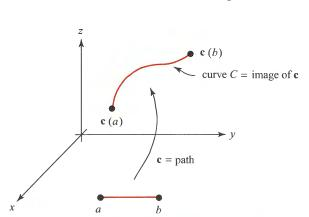
\includegraphics[width=0.6\linewidth]{figura-marsden241.jpg}
  \caption{O percurso é \(\alpha\); a sua imagem é a curva \(\mathcal{C}\)}\label{fig:241}
\end{figure}

Enfatizando estritamente, devemos distinguir entre \(\alpha(t)\) como um ponto no espaço e como um vetor baseado na origem. No entanto, não fazer isso não deve causar confusão. Vejamos algumas ideias,

Diz-se que um vetor \(\alpha\) é a função vetorial
de um argumento escalar \(t\) se cada valor do escalar escolhido
do domínio de valores admissíveis estiver associado a
um valor definido do vetor \(\alpha\). Isso pode ser escrito da seguinte forma,
\begin{equation*}
\alpha= \alpha(t). 
\end{equation*}

Se o vetor \(\alpha\) for uma função do argumento escalar \(t\),
\(\alpha =\alpha(t)\), então as coordenadas \(x\), \(y\), \(z\) do vetor \(r\) também são funções de \(t\) com valores em \(\mathbb{R}\), 
\begin{equation*}
x = x(t),\;  y = y(t),\;  z = z(t). 
\end{equation*}

Por outro lado, se as coordenadas do vetor \(\alpha\) são funções de \(t\), então o próprio vetor \(\alpha\) também é uma função de \(t\),
\begin{equation*}
\alpha = x(t)e_{1} + y(t)e_{2} + z(t)e_{3}. 
\end{equation*}

Portanto, determinar uma função vetorial \(\alpha(t)\) é o mesmo que
determinar três funções escalares ou reais \(x(t)\), \(y(t)\), \(z(t)\).

Um caminho ou percurso em \(\mathbb{R}^{n}\) é uma aplicação \(\alpha \colon [a,\; b] \to  \mathbb{R}^{n}\); é um caminho no plano se \(n=2\) e um caminho no espaço se \(n = 3\). A coleção de pontos \(\alpha(t)\) quando \(t\) varia no intervalo fechado \([a,\; b]\) é chamada de curva, e \(\alpha(a)\) e \(\alpha(b)\) são seus pontos finais. Diz-se que o caminho \(\alpha\) parametriza essa curva.

Se \(\alpha\) é um caminho em \(\mathbb{R}^{3}\), podemos escrever \(\alpha(t) = \langle x(t),\; y (t),\; z (t)\rangle \) e chamar
\(x(t)\), \(y (t)\) e \(z(t)\) de funções componentes de \(\alpha\). Distinguimos as funções de componentes de forma semelhante em \(\mathbb{R}^{2}\) ou, geralmente, em \(\mathbb{R}^{n}\).

\begin{defi}[Hodógrafo]
O hodógrafo da função vetorial \(\alpha(t)\) de um argumento escalar é o lugar geométrico descrito pelo extremo do vetor \(\alpha(t)\), à medida que o escalar 
\(t\) varia, quando a origem do vetor \(\alpha(t)\) é fixada em um ponto \(0\) no espaço. Veja Figura~\ref{fig:1-1}
\end{defi}
\begin{figure}[H]
\centering
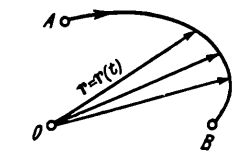
\includegraphics[width=0.5\textwidth]{hodografo-01.jpg}
\caption{Hodógrafo de uma função vetorial \(r=\alpha\)}
\label{fig:1-1}
\end{figure}

O hodógrafo de um raio vetor \(\alpha = \alpha(t)\) de um ponto em movimento é a trajetória \(\mathcal{C}\) desse ponto.
Outra reta \(\mathcal{C}_{1}\)  é o hodógrafo da velocidade \(v = v(t)\) daquele ponto. Veja a Figura~\ref{fig:1-2}
 \begin{figure}[H]
 	\centering
 	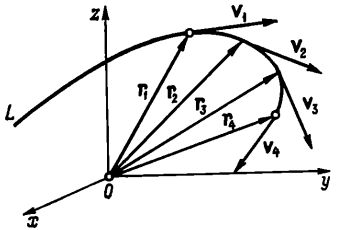
\includegraphics[width=0.5\textwidth]{hodografo-raio-vetor-01.jpg}
 	\caption{Hodógrafo \(\mathcal{C}=L\) de um raio vetor \(\alpha=\alpha(t)=r(t)\)}
 	\label{fig:1-2}
 \end{figure}

Assim, se um ponto material (partícula) está em movimento ao redor de um círculo com velocidade constante, \(\|v\|\; = \; \text{constante}\), então seu hodógrafo de velocidades é igualmente um circunferência com centro em \(0_{1}\) e raio igual a \(\|v\|\). Veja a Figura~\ref{fig:1-3}
 \begin{figure}[H]
	\centering
	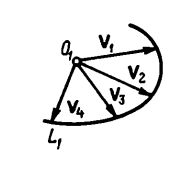
\includegraphics[width=0.5\textwidth]{hodografo-raio-vetor-02.jpg}
	\caption{Hodógrafo \(\mathcal{C}_{1}=L_{1}\) de um raio vetor \(\alpha=\alpha(t)=\text{constante}\)}
	\label{fig:1-3}
\end{figure}



\begin{exc}\label{exem:1-01}
Encontre a função vetorial que descreve 
a linha reta \(\mathcal{L}\) em \(\mathbb{R}^{3}\)  que passa
através do ponto \(P_{0}=(x_{0},\; y_{0},\; z_{0})\) na direção do vetor \(\boldsymbol{\nu}\).
\end{exc}

\solo Trata-se da  imagem do caminho ou percurso
\begin{equation*}
  \alpha(t)=P_{0}+t\,\boldsymbol{\nu}
\end{equation*}
para \(t \in \mathbb{R}\), utilizando ideias de geometria analitica, forma ponto vetor direção. Veja a Figura~\ref{fig:162}). Assim, nossa noção de curva inclui linhas retas como casos especiais. \hfill \(\lozenge\)

\begin{figure}[H]
  \centering
  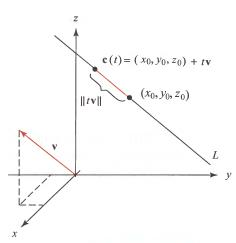
\includegraphics[width=0.45\linewidth]{figura-marsden242.jpg}
  \caption{\(\mathcal{L}\) é a linha reta no espaço através de \(P_{0}\) e na direção \(\boldsymbol{\nu}\); sua equação é
  \(\alpha(t) = P_{0} + t\,\boldsymbol{\nu}.\)}\label{fig:162}
\end{figure}

\begin{exc}\label{exe:1-02}
Encontre a função vetorial da circunferência unitária \(\mathcal{C} \colon x^{2}+y^{2}=1\) no plano \(\mathbb{R}^{2}\).
\end{exc}

\solo
Trata-se a imagem do caminho ou percurso, \(\alpha \colon \mathbb{R} \to \mathbb{R}^{2}\) definido por
\begin{equation*}
\alpha(t) =\langle \cos t, \; \sen t \rangle, \quad 0 \leq t \leq 2\pi
\end{equation*}
(veja a Figura~\ref{fig:243}).

O círculo unitário também é a imagem do caminho \(\widetilde{\alpha}(t) =
\langle \cos 2t,\; \sen 2t\rangle \), \(0 \leq t \leq \pi\). Assim, caminhos diferentes podem parametrizar a mesma curva.
\hfill \(\lozenge\)
\begin{figure}[H]
  \centering
  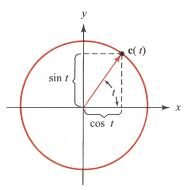
\includegraphics[width=0.3\linewidth]{figura-marsden243.jpg}
  \caption{\(\alpha(t) = \langle\cos t,\; \sen t\rangle\) é um caminho cuja imagem \(\mathcal{C}\) é a circunferência unitária.}\label{fig:243}
\end{figure}


\begin{exc}\label{exe:1-03}
O caminho o percurso \( \alpha(t) =\langle t,\; t^{2}\rangle\) traça um arco parabólico. Esta curva coincide com o gráfico de \(f(x) = x^{2}\). Veja a Figura~\ref{fig:164}.
\end{exc}

\begin{figure}[H]
  \centering
  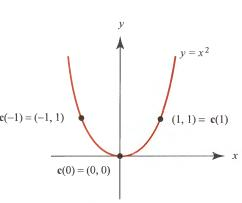
\includegraphics[width=0.4\linewidth]{figura-marsden244.jpg}
  \caption{A imagem de \(\alpha(t) =\langle t,\; t^{2}\rangle \) é a parábola \(y = x^{2}\).}\label{fig:164}
\end{figure}


\begin{exc}
Construa o hodógrafo do vetor \(\alpha=\alpha(t)\) onde 
\begin{equation*}
	\alpha(t) = t\,e_{1}+ t\,e_{2} + t^{2}e_{3}.
\end{equation*}
\end{exc}

\solo
Esta construção pode ser realizada usando pontos e montando uma tabela,
\begin{table}[H]
	\centering
	\begin{tabular}{cccccc}
		\toprule[2pt]
	\(t\)	& 0  & 1 &2  &3  &4  \\
		\midrule
	\(\alpha\)	& 0 & \(\langle 1,\; 1,\; 1 \rangle\) & \(\langle 2,\; 2,\; 4 \rangle\)  & \(\langle 3,\; 3,\; 9 \rangle\) & \(\langle 4,\; 4,\; 16 \rangle\) \\
		\bottomrule[2pt]
	\end{tabular}
\end{table}


Solução alternativa. Denote por \(x\), \(y\), \(z\) as coordenadas do vetor 
\(\alpha\); temos
\begin{equation*}
	x = t,\quad  y = t,\quad  z=t^{2}.
\end{equation*}

Eliminando o parâmetro \(t\) dessas equações, obtemos as equações das superfícies 
\begin{equation*}
	y = x, \quad  z = x^{2}, 
\end{equation*}
cuja reta \(\mathcal{L}\) de intersecção define o hodógrafo do vetor \(\alpha(t)\) Veja a Figura~\ref{fig:1-4}.
\begin{figure}[H]
\centering
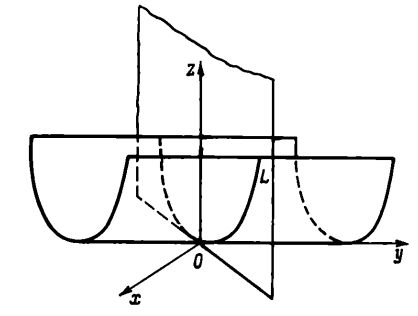
\includegraphics[width=0.5\textwidth]{curve-intersection-two-superficie.jpg}
\caption{Reta \(\mathcal{L}\) de intersecção que define o hodógrafo do vetor}
\label{fig:1-4}
\end{figure}


\begin{exc}\label{exer:5-01}
Seja \(\alpha\) uma função vetorial definida por
\begin{equation*}
\alpha(t)=\sqrt{t-3}\,\boldsymbol{i}+(t-2)^{-1}\, \boldsymbol{j}.
\end{equation*}

Identifique as funções componente e encontre o domínio comum a ambas.
\end{exc}

\solo
(a) As funções componentes \(f(t) = \sqrt{t-3}\) e \(g(t) = (t-2)^{-1}\), são funções reais.

(b) O domínio de \(\alpha\) é o conjunto de valores de \(t\) para os quais as funções \(f\)  e \(g\)
são definidas. O valor da função \(f\) é definido para t \(\geq 3\) e \(g \) é definida para todos os números reais, exceto \(2\).

Portanto, o domínio de \(\alpha\) é dado por conjunto
\begin{equation*}
\{t \; \colon \;  t \geq 3\} \cap \{t \; \colon\;  t \neq 2\}=\{t\; \colon \;  t \geq 3\quad \text{e} \quad  t \neq 2\} = \{t \in \mathbb{R}\colon t \geq 3\}.
\end{equation*}

\begin{exc}\label{exer:5-02}
Seja dada uma função vetorial definida por
\begin{equation*}
  \alpha(t)=2\cos t\,\boldsymbol{i}+ 2\sen t\, \boldsymbol{j}.
\end{equation*}

\rm{(a)} Encontre o domínio da função vetorial;  \rm{(b)} Faça um esboço do gráfico dessa equação;  \rm{(c)} Encontre a equação cartesiana do gráfico.
\end{exc}

\solo
(a) O domínio de \(\alpha\) é o conjunto de todos os números reais. Poderíamos tabular os valores de \(x\) e \(y\) para valores particulares de \(t\).

(b) Calculemos a magnitude ou módulo  do vetor posição, temos para cada \(t\)
\begin{equation*}
\|\alpha(t)\| = \sqrt{4 \cos^{2} t + 4 \sen^{2} t} = 2 \sqrt{\cos^{2} t + \sen^{2} t} = 2.
\end{equation*}

Portanto, o ponto final da representação da posição de cada vetor \(\alpha(t)\) está a duas unidades da origem.

Ao deixar \(t\) assumir todos os números no intervalo fechado \([0,\; 2\pi]\), obtemos uma circunferência com seu centro na origem e raio \(2\). Com isto completamos o gráfico inteiro porque qualquer valor de \(t\) dará um ponto nesta circunferência. Um esboço do círculo é mostrado na Figura~\ref{fig:1541}.

As equações paramétricas do gráfico são
\begin{equation*}
x = 2 \cos t \quad \text{e}\quad  y = 2\sen t
\end{equation*}

(c) Uma equação cartesiana do gráfico pode ser encontrada eliminando o parâmetro \(t\) das duas equações paramétricas, que ao elevar os dois lados de cada equação ao quadrado e adicionar
\begin{equation*}
x^{2} + y^{2} = 4
\end{equation*}

\begin{figure}[H]
  \centering
  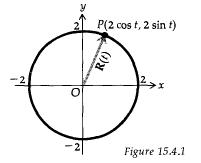
\includegraphics[width=0.4\linewidth]{figura-leithold1541.jpg}
  \caption{Esboço da curva circunferência com \(\alpha(t)=R(t)\)}\label{fig:1541}
\end{figure}


\begin{exc}\label{exer:5-03}
Dadas as equações paramétricas
\begin{equation*}
  x=\cosh t \quad \text{e}\quad y = \senh t
\end{equation*}
\((a)\) Faça um esboço do gráfico dessa equação \((b)\) Encontre a equação cartesiana do gráfico \((c)\) Encontre o domínio
da função vetorial dada.
\end{exc}

\solo
(a) Elevando ao quadrado em ambos os lados das equações dadas e subtraindo, teremos
\begin{equation*}
x^{2}-y^{2} = \cosh^{2} t - \senh^{2} t
\end{equation*}

A partir da identidade \(\cosh^{2} t - \senh^{2} t = 1\), esta equação torna-se
\begin{equation*}
x^{2}-y^{2} = 1
\end{equation*}

A equação resultante é uma equação de uma hipérbole equilátera. Entretanto observe que para todo \(t\) número real,
\(\cosh t\) nunca é menor do que \(1\).

Assim, a curva definida pelas equações paramétricas consiste apenas nos pontos do ramo direito da hipérbole. Um esboço dessa curva é mostrado na Figura~\ref{fig:1543}.

(b) Uma equação cartesiana é
\begin{equation*}
x^{2} - y^{2} = 1, \quad  \text{onde} \quad  x> 1.
\end{equation*}

\begin{figure}[H]
  \centering
  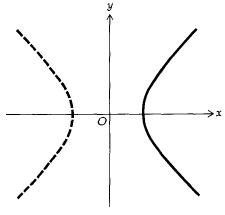
\includegraphics[width=0.4\linewidth]{figura-leithold1543.jpg}
  \caption{Equação Cartesiana do gráfico}\label{fig:1543}
\end{figure}


\bigskip
\noindent\textbf{Observação.}
Conforme afirmado anteriormente, ao eliminar \(t\) das equações paramétricas obtemos uma equação cartesiana. A equação cartesiana resultante, implícita ou explicitamente, define \(y\) como uma ou mais funções dependentes de \(x\).

Ou seja, se \(x = f(t)\) e \(y = g(t)\), então \(y = h(x)\). Se \(h\) é uma função diferenciável de \(x\) e \( f\) é uma função diferenciável de \(t\), segue-se da regra da cadeia usando operadores
\begin{equation*}
D_{t}y = \left(D_{x}y\right)\, \left( D_{t}x\right)
\end{equation*}
ou
\begin{equation*}
g'(t) = (h'(x))\,(f'(t))
\end{equation*}
ou, usando notação diferencial,
\begin{equation*}
\frac{dy}{dt}=\frac{dy}{dx}\,\frac{dx}{dt}
\end{equation*}

Se \(dx/dt \neq 0\), podemos dividir em ambos os lados da equação acima por \(dx/dt\) e obter
\begin{equation}\label{eq:14-3-2}
\frac{dy}{dx}= \dfrac{\dfrac{dy}{dt}}{\dfrac{dx}{dt}}
\end{equation}

A equação \eqref{eq:14-3-2} nos permite encontrar a derivada de \(y\) em relação a \(x\) diretamente a partir das equações paramétricas.

Por outro lado, obtemos a segunda derivada de \(y\) utilizando as equações paramétricas
\begin{equation*}
  \frac{d^{2}y}{dx^{2}}= \frac{d}{dx}\left(\frac{dy}{dx} \right)
\end{equation*}
então
\begin{equation*}
  \frac{d^{2}y}{dx^{2}}=\frac{d}{dx}\left( y'\right)
\end{equation*}

Assim, substituindo a fórmula da primeira derivada, obtemos a fórmula para a segunda derivada,
\begin{equation*}
  \frac{d^{2}\,y}{dx^{2}}= \dfrac{\dfrac{dy'}{dt}}{\dfrac{dx}{dt}}
\end{equation*}

\begin{exc}\label{exer:14-3-3}
Dados as equações paramétricas
\begin{equation*}
x = 3t^{2}\quad \text{e} \quad y = 4t^{3},
\end{equation*}
encontre \(dy/dx\) e \(d^{2}y/dx^{2}\) sem eliminar o parâmetro \( t\).
\end{exc}

\solo
Calculando as derivadas do numerador e denominador da fórmula,
\begin{equation*}
\frac{dy}{dt}= 12t^{2}, \qquad \frac{dx}{dt}=6t \neq 0
\end{equation*}

Substituindo na fórmula deduzida anteriormente,
\begin{equation*}
  \frac{dy}{dx}=\frac{12t^{2}}{6t}=2t.
\end{equation*}

Para calcular a segunda derivada, usando o resultado da primeira derivada \(dy/dx=y'=2t\) e assim,
\begin{equation*}
  \frac{d\, y'}{dt}=\frac{d}{dt}2t=2.
\end{equation*}

Então, novamente substituindo na fórmula,
\begin{equation*}
  \frac{d^{2}}{dx^{2}}=\dfrac{\dfrac{d(y')}{dt}}{\dfrac{dx}{dt}}=\frac{2}{6t}=\frac{1}{3t}, \quad t \neq 0
\end{equation*}


\begin{exc}\label{exer:14-3-4}
Escreva os detalhes da resolução dos itens
\begin{enumerate}
  \item[\rm{(a)}]
Desenhe um esboço do gráfico da curva definida por as equações paramétricas
\begin{equation*}
x = f(t) = 3t^{2} \quad \text{e}\quad y = g(t)=4t^{3}
\end{equation*}
  \item[\rm{(b)}] Encontre uma equação cartesiana do gráfico.
\end{enumerate}
\end{exc}

\solo
Sabemos a forma das equações paramétricas, a saber,
\begin{equation*}
x=f(t)= 3t^{2} \quad \text{e}\quad y = g(t)=4t^{3}
\end{equation*}

\begin{enumerate}
\item[(a)]
Como \(x = 3t^{2}\), concluímos que \(x\) nunca é negativo. Assim o gráfico esta confinado no primeiro e quarto quadrante. A Tabela~\ref{tab:1541}
fornece os valores de \(x\) e\(y\) para valores particulares de \(t\).
\begin{table}[H]
\centering
\begin{tabular}{m{5em} m{5em} m{5em}}
	\toprule[2pt]
\(t\)	& \(x\) & \(y\) \\
	\midrule[1.5pt]
0	& 0 & 0  \\
	\midrule
1/2	& 3/4 & 1/2  \\
	\midrule
1	& 3 & 4 \\
	\midrule
2	& 12 & 32  \\
	\midrule
-1/2	&3/4  & -1/2  \\
	\midrule
-1	&3  & -4 \\
	\midrule
-2	& 12 & -32 \\
	\bottomrule[2.0pt]
\end{tabular}
 \caption{Tabela com valores particulares de \(t\)}\label{tab:1541}
\end{table}

Como \(D_{x}y = 2t\), então que quando \(t = 0\), obtemos \(D_{x}y = 0\); portanto, a reta tangente é horizontal no ponto origem \((0,\; 0)\). Um esboço do gráfico é mostrado na Figura~\ref{fig:1542}.
\begin{figure}[H]
\centering
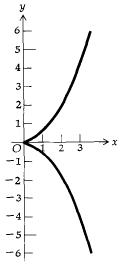
\includegraphics[width=0.2\linewidth]{figura-leithold1542.jpg}
\caption{Esboço do Gráfico das equações Paramétricas}\label{fig:1542}
\end{figure}

\item[(b)]
A partir das duas equações paramétricas \(x = 3t^{2}\) e \(y = 4t^{3}\), obtemos
\begin{equation*}
x^{3} = 27\,t^{6} \quad \text{e} \quad y^{2} = 16\,t^{6}.
\end{equation*}

Resolvendo essa equações para o valor \(t^{6}\) e posteriormente eliminado \( t^{6}\), obtemos,
\begin{equation*}
  \frac{x^{3}}{27}=\frac{y^{2}}{16} \quad \Rightarrow \quad 16\, x^{3} = 27\, y^{2}
\end{equation*}
qual é a equação cartesiana desejada.
\end{enumerate}

O que acontece se derivamos implicitamente a equação cartesiana obtida no item (b)
\begin{equation*}
  48x^{2}=54\,y\,\frac{dy}{dx}\quad \Rightarrow \quad \frac{dy}{dx}=\frac{8x^{2}}{9y}
\end{equation*}

Substituindo \(x\) e \(y\) em termos do parâmetro \(t\) a partir das equações paramétricas fornecidas, obtemos
\begin{equation*}
  \frac{dy}{dx}=\frac{8x^{2}}{9y}=\frac{8(3t^{2})^{2}}{9(4t^{3}}=\frac{72t^{4}}{36t^{3}}=2t
\end{equation*}
o resultado obtido coincide com el valor fornecido pela fórmula de derivação  a 
partir das equações paramétricas, isto é sem conhecer o formato cartesiano da 
função.

%
\section{Cálculo com Funções Vetoriais}
%
Todas as definições de limites, continuidade, derivação e integração indefinida de funções com valores vetoriais envolvem as definições
correspondentes para funções reais do Cálculo Diferencial.

Suponha que uma função vetorial \(\alpha=\alpha(t)\) de um argumento escalar \(t\) 
seja definida em alguma vizinhança do valor \(t_{1}\) do argumento \(t\), exceto 
talvez para o próprio valor \(t_{1}\).

Um vetor constante \(B\) é dito ser o limite do vetor \(\alpha(t)\), quando  
\(t\to t_{1}\), se para qualquer \(\varepsilon > 0\) existe um \(\delta > 0\) tal que para todos os \(t \neq  t_{1}\) que satisfazem a condição \(0< |t-t_{1}|< \delta\) a seguinte desigualdade é verdadeira,
\begin{equation*}
\left|\alpha(t)-B\right| < \varepsilon.
\end{equation*}

Como no caso do cálculo I, escrevemos
\begin{equation*}
 \lim_{t \to t_{1}}\alpha(t)=B.
\end{equation*}

Geometricamente, isso significa que o vetor \(\alpha(t)\) tende, quando \(t\to t_{1}\), ao vetor B tanto em comprimento quanto em direção. Veja a Figura~\ref{fig:1-5}
\begin{figure}[H]
\centering
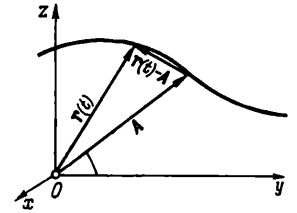
\includegraphics[width=0.5\textwidth]{limite-vetorial.jpg}
\caption{Interpretação geometricamente do limite}
\label{fig:1-5}
\end{figure}

\begin{defi}[Limite em termos de Componentes]\label{def:14-4-1}
Seja \(\alpha\) uma função com valor vetorial, cujos valores de função são dados por
\begin{equation*}
\alpha(t) = f(t)\,e_{1} + g(t)\,e_{2}= f(t)\,\boldsymbol{i} + g(t)\, \boldsymbol{j}.
\end{equation*}

Então, o limite de \(\alpha(t)\) quando \(t\) se aproxima de \(t_{1}\) é definido por
\begin{equation*}
  \lim_{t \to t_{1}}\alpha(t) =\left[\lim_{t \to t_{1}}f(t)\right]e_{1}+ \left[ \lim_{t \to t_{1}}g(t)\right]e_{2}
\end{equation*}
se \(\lim f (t)\) e \(\lim g (t)\) existem quando \( t \to t_{1}\).
\end{defi}

\begin{exc}
  Encontre o limite função vetorial,
  \begin{equation*}
    \alpha(t) = \frac{1-\sqrt{t+1}}{1-t}e_{1} + \frac{t}{t+1}e_{2}\quad \text{ quando} \quad t_{1}=0
  \end{equation*}
\end{exc}

\solo
Como cada função componente possui limite em \(t_{1}\), logo existe o limite da função vetorial, isto,
\begin{equation*}
  \lim_{t \to t_{1}}\frac{1-\sqrt{t+1}}{1-t}=\lim_{t \to 0}\frac{1-\sqrt{t+1}}{1-t}=0
\end{equation*}

Por outro lado calculamos o limite da função racional
\begin{equation*}
\lim_{t \to t_{1}}\frac{t}{t+1}=\lim_{t \to 0}\frac{t}{t+1}=0
\end{equation*}

Finalmente o limite da função vetorial
\begin{equation*}
\lim_{t \to 0}\alpha(t) = \lim_{t \to 0}\frac{1-\sqrt{t+1}}{1-t}\,e_{1} + \lim_{t \to 0}\frac{t}{t+1}\, e_{2}
\end{equation*}
e como cada limite da funções componentes foi calculado temos,
\begin{equation*}
\lim_{t \to 0}\alpha(t) = 0\,e_{1}+0\,e_{2}=(0, \; 0).
\end{equation*}

\begin{defi}[Continuidade]\label{def:14-4-2}
A função de valor vetorial \(\alpha\) é contínua no ponto \(t_{1}\) se e somente se as três condições a seguir forem
satisfeitas;
\begin{tasks}[label=(\alph*),item-indent=4em,label-width=4ex,ref=(\alph*)](2)
\task \(\alpha(t_{1})\) existe;
\task existe \(\lim \alpha(t)\), quando \(t \to t_{1}\);
\task \(\lim \alpha(t) =\alpha(t_{1})\) quando \( t \to t_{1}\).
\end{tasks}
\end{defi}

%
\subsection*{Observação Importante}
%
A partir  Definição~\ref{def:14-4-1} e Definição~\ref{def:14-4-2}, segue-se que a função vetorial \(\alpha\), definida por
\begin{equation*}
\alpha(t) = f(t)\, e_{1} + g(t)\, e_{2},
\end{equation*}
é contínua em \(t_{1}\) se e somente se \(f\) e \(g\) forem contínuas em \(t_{1}\).

Suponha que uma função vetorial \(\alpha = \alpha(t)\) seja definida para todo \(t\) no intervalo \(]a,\; b[\). Tome algum valor \(t \in\; ]a,\; b[\), então dê a \(t\) um incremento \(\Delta t\) tal que \(t+\Delta t \in\; ]a,\; b[\) e encontre o incremento correspondente 
\(\Delta \alpha = \alpha(t + \Delta t) - \alpha(t)\) na função vetorial \(\alpha(t)\). Agora considere a razão 
\begin{equation*}
	\dfrac{\Delta \alpha }{\Delta t}.
\end{equation*}

Se, a razão \(\Delta \alpha/\Delta t\) tem um limite, quando  \(\Delta t\to 0\) então esse limite é chamado de \texttt{derivada} da função vetorial \(\alpha = \alpha(t)\) em relação ao argumento escalar \(t\) para um dado valor \(t\) do argumento e é denotado como \(d\alpha(t)/dt\) ou \(\alpha'(t)\) ou \(\dot{\alpha}(t)\). Assim,
\begin{equation*}
\dfrac{d}{dt}\alpha(t) = \lim_{\Delta t \to 0}\dfrac{\Delta \alpha }{\Delta t}=
\lim_{\Delta t \to 0}\dfrac{\alpha(t+\Delta t)-\alpha(t)}{\Delta t}.
\end{equation*}

Neste caso, a função vetorial \(\alpha=\alpha(t)\) é dita diferenciável.


\begin{defi}[Derivada]\label{def:14-4-3}
Se \(\alpha\) é uma função vetorial, então a derivada de \(\alpha\) é outra função  vetorial, denotada por \(\alpha'\) e definida por
\begin{equation*}
  \alpha'(t)= \lim_{\Delta t\to 0}\frac{\alpha(t+\Delta t) -\alpha(t)}{\Delta t}
\end{equation*}
se esse limite existir.
\end{defi}

Na definição anterior, a expressão
\begin{equation*}
\frac{\alpha(t+\Delta t) -\alpha(t)}{\Delta t}
\end{equation*}
foi usada para representar divisão de um vetor por um escalar que ainda não foi definida. Por esta expressão queremos
dizer
\begin{equation*}
  \frac{1}{\Delta t}\left[\alpha(t+\Delta t) -\alpha(t)\right]
\end{equation*}

A notação com operadores \(D_{t}\alpha(t)\) às vezes é usada no lugar de \(\alpha'(t)\).

Uma interpretação geométrica da Definição~\ref{def:14-4-3} é obtida por considerando representações dos vetores
\(\alpha(t)\), \(\alpha(t + h)\) e \( \alpha'(t)\). Consulte a Figura~\ref{fig:1551}.

\begin{figure}[!h]
  \centering
  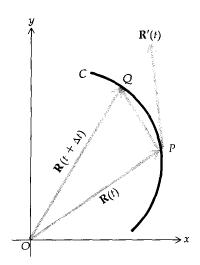
\includegraphics[width=0.3\linewidth]{figura-leithold1551.jpg}
  \caption{Representação Geométrica da derivação de funções Vetoriais}\label{fig:1551}
\end{figure}

A curva \( \mathcal{C}\) é traçada pelo ponto final da representação da posição de \(\alpha(t)\), pois \(t\) assume todos os valores no domínio de \(\alpha\). Seja \(\overrightarrow{OP}\) a representação da posição de \(\alpha(t)\) e \(\overrightarrow{OQ}\) seja a representação da posição de \(\alpha(t+\Delta t)\). Então \(\alpha(t + \Delta t)-\alpha(t)\) é um vetor para o qual \(\overrightarrow{PQ}\) é uma representação. Se o vetor \(\alpha(t + \Delta t)-\alpha(t)\) é multiplicado pelo escalar \(1/\Delta t\), obtemos um vetor com a mesma direção e cuja magnitude é \(1/\Delta t\) vezes a magnitude de \(\alpha(t + \Delta t) - \alpha(t)\).

À medida que \(\Delta t\) se aproxima de zero, o vetor \([\alpha(t + \Delta t)-\alpha(t)]/\Delta t\) se aproxima de um vetor tendo uma de suas representações tangente à curva \( \mathcal{C}\) no ponto \(P\).

O seguinte teorema segue da Definição~\ref{def:14-4-3} e da definição da derivada de uma função real.
\begin{teo}\label{thm:14-4-4}
Se \(\alpha\) é uma função  vetorial definida por
\begin{equation*}
\alpha(t) = f(t)\,e_{1} + g(t)\,e_{2}
\end{equation*}
então
\begin{equation*}
\alpha'(t) = f'(t)\,e_{1} + g'(t)\,e_{2}
\end{equation*}
se \(f'(t)\) e \(g'(t)\) existirem.
\end{teo}

Derivadas de ordem superior de funções com valor vetorial são definidas como derivadas de ordem superior de funções com valor real. Portanto, se \(\alpha\) é uma função de valor vetorial definida por
\begin{equation*}
\alpha(t) = f(t)\,i + g(t)\, j,
\end{equation*}
a segunda derivada de \( \alpha\), denotada por \( \alpha''(t)\), é dada por
\begin{equation*}
\alpha''(t) = D_{t}[\alpha'(t)]
\end{equation*}

Também temos a notação \(D_{t}^{2}\alpha(t)\) no lugar de \(\alpha''(t)\). Aplicando o Teorema~\ref{thm:14-4-4} a \(\alpha'(t)\), obtemos
\begin{equation*}
\mathbf{a}(t)=\alpha''(t) = f''(t)\, i + g''(t)\,j
\end{equation*}
se \(f''(t)\) e \(g''(t)\) existirem.

Se pensarmos em \(\alpha(t)\) como o caminho traçado por uma partícula e como \(t\) é o tempo, é razoável definir o vetor velocidade da seguinte
maneira.

\noindent\textbf{Vetor de Velocidade.}
A velocidade de um caminho \(\alpha\) é definida por
\begin{equation*}
  \alpha'(t)=\lim_{\Delta t \to 0}\frac{\alpha(t+\Delta t)-\alpha(t)}{\Delta t}
\end{equation*}

Normalmente desenhamos o vetor \(\alpha'(t)\) com seu inicio no ponto \(\alpha(t)\). A velocidade do caminho \(\alpha(t)\) é \(s =|\alpha'(t)|\), o comprimento do vetor velocidade. Se \(\alpha(t) = \langle x(t), \; y(t) \rangle\) em \(\mathbb{R}^{2}\), então
\begin{equation*}
\alpha'(t) = \langle x'(t),\; y'(t)\rangle = x'(t)\,i+ y'(t)\,j=x'(t)\,e_{1}+ y'(t)\,e_{2}
\end{equation*}
e se \(\alpha(t) = \langle x(t), \; y (t), \; z'(t)\rangle\) em \(\mathbb{R}^{3}\), então
\begin{equation*}
\alpha'(t) = \langle x'(t),\; y'(t),\; z(t)\rangle= x'(t)\,i+ y'(t)\,j+z'(t)\, k=x'(t)\,e_{1}+ y'(t)\,e_{2}+z'(t)\,e_{3}
\end{equation*}

A teoria dos limites segue a ideia do cálculo de uma variável. Aqui, \(x'(t)\) é a derivada de uma variável comum \(dx/dt\). Se aceitarmos limites de vetores interpretados por componentes, as fórmulas para o vetor velocidade vêm da definição da derivada.

No entanto, o limite também pode ser interpretado no sentido de vetores. Na Figura~\ref{fig:248}, vemos que
\begin{equation*}
\frac{\alpha(t + \Delta t)-\alpha(t)}{\Delta t}\quad  \text{se torna tangente à curva quando}\quad  \Delta t \to 0.
\end{equation*}

\begin{figure}[!h]
  \centering
  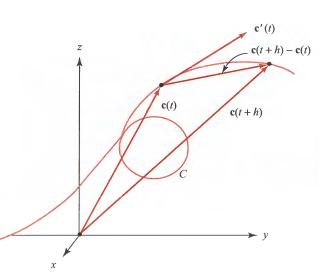
\includegraphics[width=0.5\linewidth]{figura-marsden248.jpg}
  \caption{O vetor \(\alpha'(t)\) é tangente ao caminho \(\alpha(t)\).}\label{fig:248}
\end{figure}

%
\noindent\textbf{Vetor Tangente.}
%
A velocidade \(\alpha'(t)\) é um vetor tangente ao caminho \(\alpha(t)\) no tempo \(t\). Se \(\mathcal{C}\) for uma curva traçada por \(\alpha\) e se \(\alpha'(t)\) não for igual a \(0\), então \(\alpha'(t)\) é um vetor tangente à curva \(\mathcal{C}\) no ponto \(\alpha(t)\).

A velocidade \(\alpha'(t)\) é um vetor tangente ao caminho \(\alpha(t)\). Se pensarmos na derivada \(D\alpha(t)\) como uma matriz, ela será um vetor coluna com as entradas \(x'(t)\), \(y'(t)\) e \(z'(t)\), isto é,
\begin{equation*}
  D\alpha(t)=\left[
  \begin{array}{c}
  x'(t)\\
  y'(t)\\
  z'(t)
  \end{array}
  \right]
\end{equation*}

Lembre-se de que um caminho em $\mathbb{R}^{n}$ é uma função $\alpha$ de $\mathbb{R}$ ou um intervalo $J$ de $\mathbb{R}$ a $\mathbb{R}^{n}$. Se o
caminho é diferenciável, sua derivada em cada instante $t$ é uma matriz $n\times 1$. Especificamente, se $x_{1}(t),\ldots,x_{n}(t)$ são as funções componentes de $\alpha$, a matriz derivada é
\begin{equation*}
\alpha'(t)=\begin{bmatrix}
               \dfrac{d}{dt}x_{1}(t) \\[2ex]
               \dfrac{d}{dt}x_{2}(t)\\[2ex]
               \vdots \\[2ex]
               \dfrac{d}{dt}x_{n}(t)
             \end{bmatrix}
\end{equation*}
que também pode ser escrito em forma de vetor como
\begin{equation*}
\left\langle \frac{d}{dt}x_{1}(t),\; \frac{d}{dt}x_{2}(t), \ldots, \frac{d}{dt}x_{n}(t)\right\rangle \quad \text{ou}\quad \left\langle x'_{1}(t), \; x'_{2}(t), \ldots, x'_{n}(t)\right\rangle.
\end{equation*}

Lembre-se de que $\alpha'(t)$ é o vetor tangente ao percurso no ponto $\alpha(t)$. Lembre-se também de que se $\alpha$ representa o percurso de uma
partícula em movimento, então seu vetor de velocidade é
\begin{equation*}
  v=\alpha'(t)
\end{equation*}
e sua velocidade é $s =\|v\|$. Portanto, a derivada pensada é consistente com nossa noção anterior.

\bigskip
\begin{exc}\label{exer:1-05}
Calcule o vetor tangente ao caminho
\begin{equation*}
\alpha(t) =\langle t,\; t^{2},\; e^{t}\rangle \quad \text{em}  \quad t = 0;
\end{equation*}
\end{exc}

\solo
Derivando uma vez \(\alpha\) obtemos
\begin{equation*}
\alpha'(t) = \langle 1,\; 2t,\; e^{t}\rangle,
\end{equation*}
e assim em \(t=0\) obtemos o vetor tangente representado pela tripla \(\langle 1,\;0,\;1\rangle\).

\begin{exc}\label{exer:1-06}
Descreva o caminho $\alpha(t) = \langle \cos t,\; \sen t,\; t \rangle$. Encontre o vetor de velocidade no ponto da curva imagem onde \(t = \pi/2\).
\end{exc}

\solo Para um dado \(t\), o ponto \((\cos t,\; \sen t,\; 0)\) está no círculo \(x^{2} + y^{2} = 1\) no plano \(xy\). Portanto, o ponto \(\langle \cos t,\; \sen t,\; t\rangle \) encontra-se \(t\) unidades acima do ponto \(\langle \cos t,\; \sen t,\; 0\rangle \) se \(t\) for positivo e \(-t\) unidades abaixo \(\langle \cos t,\; \sen t,\; 0\rangle\) se \(t\) for negativo.

À medida que \(t\) aumenta, \(\langle \cos t,\; \sen t,\; t\rangle \) envolve o cilindro \(x^{2} + y^{2} = 1\) com o aumento da coordenada \(z\).

A curva que isso traça é chamada de \textbf{hélice}, que é representada na Figura~\ref{fig:249}. Em \(t = \pi/2\),
\begin{equation*}
\alpha'(\pi/2) = \left\langle -\sen \frac{\pi}{2}, \cos \frac{\pi}{2},\; 1\right\rangle=\langle-1,\; 0,\; 1\rangle = -i + k.
\end{equation*}

\begin{figure}[H]
  \centering
  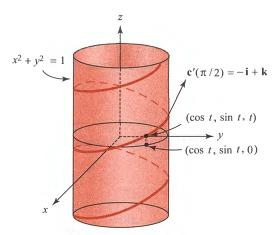
\includegraphics[width=0.5\linewidth]{figura-marsden249.jpg}
  \caption{A hélice \(\alpha(t) = (\cos t,\; \sen t,\; t)\) envolve o cilindro \(x^{2}+y^{2} = 1\).}
  \label{fig:249}
\end{figure}

%
\subsection*{Reta Tangente a um Percurso.}
%
A reta tangente a um caminho em um ponto é a reta que passa pelo ponto na direção do vetor tangente. Usando a forma ponto-direção da equação de uma reta, obtemos a equação paramétrica para a reta tangente.

Se \(\alpha(t)\) é um caminho, sua reta tangente no ponto \(\alpha(t_{0})\) é
\begin{equation*}
l(t) =\alpha(t_{0}) + (t-t_{0})\alpha'(t_{0}).
\end{equation*}

Por conveniência, escrevemos a equação de forma que \(l\) passe por \(\alpha(t_{0})\) em \(t = t_{0}\) (em vez de \(t = 0\)). Veja a Figura~\ref{fig:2411}

\begin{figure}[H]
  \centering
  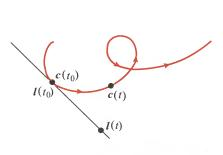
\includegraphics[width=0.5\linewidth]{figura-marsden2411.jpg}
  \caption{A reta tangente a um caminho.}\label{fig:2411}
\end{figure}

\begin{exc}\label{exer:1-07}
Um caminho em \(\mathbb{R}^{3}\) passa pelo ponto \((3,\; 6,\; 5)\) em \(t = 0\) com vetor tangente \(i -j\). Encontre a equação da reta tangente.
\end{exc}

\solo A equação da reta tangente pela definição é
\begin{equation*}
l(t) = (3,\; 6,\; 5) + t(i - j) = (3,\; 6,\; 5) + t (1,\; -1,\; 0) = (3 + t,\; 6 - t,\; 5).
\end{equation*}

Nas coordenadas \((x,\; y,\; z)\), a reta tangente é \(x = 3 + t\), \(y = 6 - t\), \(z = 5\).

Fisicamente, podemos interpretar o movimento ao longo da reta tangente como o caminho que uma partícula em uma curva seguiria se fosse liberada em um determinado momento.

\begin{exc}\label{exer:1-08}
Suponha que uma partícula siga o caminho \(\alpha(t)=\langle e^{t},\; e^{-t},\; \cos t\rangle \) até que voe pela tangente em \(t=1\). Onde se encontra em \(t=3\)?
\end{exc}

\solo Após a derivação de \(\alpha\) obtemos o vetor velocidade,
\begin{equation*}
(e^{t}, \; -e^{-t},\;  -\sen t),
\end{equation*}
que em \(t = 1\) é o vetor \((e,\; -1/e, -\sen 1)\). A partícula está em \((e,\; 1/e,\; \cos 1)\) em \(t=1\).

A equação da reta tangente é
\begin{equation*}
l(t) = \left(e,\; \frac{1}{e}, \cos 1\right) + (t - 1) \left(e,\; -\frac{1}{e},\; -\sen 1\right).
\end{equation*}

Em \(t = 3\), a posição nesta linha é
\begin{equation*}
l(3)=\left(e,\; \dfrac{1}{e},\; \cos 1 \right)+2\left( e,\; \dfrac{1}{e},\; -\sen 1 \right)=\left(3e,\;-\frac{1}{e}, \; \cos 1-2\sen 1  \right)
\end{equation*}
e assim conclui-se o exercício. \hfill $\lozenge$


\begin{exc}
Calcular a segunda derivada das seguintes funções vetoriais,
\begin{align*}
\rm{(a)} & \quad \alpha(t)=(4+\sen t)\, i + \cos t\, j \quad &\rm{(b)}&\quad \beta(t)=\ln t\, i + (1/t) \, j
\end{align*}
\end{exc}

\solo
Derivando as funções vetoriais utilizando as regras de derivação
\begin{enumerate}
  \item[(a)]
  \begin{equation*}
    \alpha'(t)=\cos t\, i -\sen t\, j
  \end{equation*}
  e segunda derivada resulta em
\begin{equation*}
    \alpha''(t)=-\sen t\, i -\cos t\, j
  \end{equation*}

  \item[(b)]
  \begin{equation*}
\beta'(t)=(1/t)\, i - (1/t^{2}) \, j
  \end{equation*}
e a sua segunda derivada,
  \begin{equation*}
\beta''(t)=-(1/t^{2})\, i +(2/t^{3}) \, j
  \end{equation*}
\end{enumerate}


\begin{defi}\label{def:14-5-5}[Derivada num intervalo]
Uma função de valor vetorial \(\alpha\) é dita como diferenciável em um intervalo se \(\alpha'(t)\) existe para todos
os valores de \(t\) no intervalo.
\end{defi}

Os teoremas a seguir fornecem fórmulas de diferenciação para funções com valor vetorial. As provas são baseadas no
Teorema~\ref{thm:14-4-4} e teoremas sobre diferenciação de funções de valor real.
\begin{teo}[Derivada da Soma]\label{thm:14-5-6}
Se \(\alpha\) e \(\beta\) são funções com valor vetorial diferenciável em um intervalo, então \(\alpha + \beta\) é
diferenciável no intervalo, e
\begin{equation*}
D_{t}[\alpha(t) +\beta(t)] = D_{t}\alpha(t) + D_{t}\beta(t)
\end{equation*}
\end{teo}

A prova desse teorema é deixada para o estudante da disciplina.

\begin{exc}
Calcule por separado cada lado da conclusão do Teorema~\ref{thm:14-5-6} para duas funções vetoriais dadas por,
\begin{equation*}
\alpha(t)=t^{2}\, i +(t-2)\,j \quad \text{e} \quad  \beta(t)=\sen t\, i+\cos t\, j.
\end{equation*}
\end{exc}

\solo
Primeiro somando a duas funções vetoriais, componente a componente
\begin{equation*}
  \alpha(t)+\beta(t)=(t^{2}+\sen t)\, i + (t-2+\cos t)\,j
\end{equation*}

Derivando a soma \( \alpha+ \beta\) temos,
\begin{equation*}
D_{t}[\alpha(t)+\beta(t)]=D_{t}[\alpha(t)]\, i +D_{t}[\beta(t)]\, j=(2t+\cos t)\, i +(1-\sen t)\, j
\end{equation*}

Por outro lado derivando separadamente cada função vetorial,
\begin{equation*}
  D_{t}[\alpha(t)]=(2t)\, i + j\quad \text{e}\quad D_{t}[\beta(t)]=\cos t\, i -\sen t\, j
\end{equation*}

Calculando a soma de derivadas,
\begin{equation*}
  D_{t}[\alpha(t)]+D_{t}[\beta(t)] = (2t+\cos t)\, i +(1-\sen t)\, j
\end{equation*}

Assim sendo temos verificado a válido a fórmula da conclusão do Teorema, isto é,
\begin{equation*}
D_{t}[\alpha(t) +\beta(t)] = D_{t}\alpha(t) + D_{t}\beta(t)
\end{equation*}


\begin{teo}\label{thm:14-4-7}
Se \( \alpha\) e \(\beta\) são funções com valor vetorial diferenciável em um intervalo, então \(\alpha \cdot \beta\)
é diferenciável no intervalo, e
\begin{equation*}
D_{t}[\alpha(t) \cdot \beta(t)] = [D_{t}\alpha(t)]\cdot \beta(t) + \alpha(t)\cdot  [D_{t}\beta(t)]
\end{equation*}
\end{teo}

\begin{exc}
Considere as funções vetoriais dadas por,
\(\alpha(t)=t^{2}\, i +(t-2)\,j \) e \(\beta(t)=\sen t\, i+\cos t\, j \). Verificar a validade da conclusão do Teorema~\ref{thm:14-4-7}
\end{exc}

\solo
Se observa que nas hipóteses do teorema existe a operação de produto interno de funções vetoriais. Portanto devemos calcular o produto interno logo derivar, isto é,
\begin{equation*}
\alpha(t) \cdot \beta(t)=(t^{2},\; (t-2))\cdot (\sen t, \;\cos t )=t^{2}\sen t+(t-2)\cos t
\end{equation*}

A seguir derivamos a função real  resultante,
\begin{equation*}
D_{t}[\alpha(t) \cdot \beta(t)]=D_{t}[t^{2}\sen t+(t-2)\cos t]=(t^{2}+1)\cos t +(t+2)\sen t
\end{equation*}

Derivando por separado cada função vetorial, obtemos
\begin{equation*}
D_{t}[\alpha(t)]=2t\,i+j \quad \text{e}\quad D_{t}[\beta(t)]=\cos t\, i -\sen t\, j
\end{equation*}

Logo temos a soma derivadas das funções vetoriais com as funções respectivamente, isto é,
\begin{equation*}
[D_{t}\alpha(t)]\cdot \beta(t)=(2t\, i +j)\cdot(\sen t\, i+ \cos t\, j )=2t\sen t+ \cos t
\end{equation*}
e o segundo produto,
\begin{equation*}
\alpha(t)\cdot  [D_{t}\beta(t)]=[t^{2}\, i +(t-2)\, j]\cdot (\cos t\, i-\sen t\, j)=t^{2}\cos t-(t-2)\sen t
\end{equation*}

Somando os resultados obtido em cada somando,
\begin{equation*}
[D_{t}\alpha(t)]\cdot \beta(t)+\alpha(t)\cdot  [D_{t}\beta(t)]=(t^{2}+1)\cos t + (t+2)\sen t.
\end{equation*}

Assim obtemos a igualdade desejada.

\begin{teo}\label{thm:14-4-8}
Se \(\alpha\) é uma função com valor vetorial diferenciável em um intervalo e \(f\) é uma função com valor real diferenciável no intervalo, então
\begin{equation*}
D_{t}({[f(t)][\alpha(t)]} = [D_{t}f(t)]\alpha(t) + f(t)D_{t}\alpha(t)
\end{equation*}
\end{teo}

A prova é deixada para o estudante da disciplina.

A seguir temos a regra da cadeia para funções vetoriais, sua justificação esta baseada na derivada de uma função vetorial e a regra da cadeia de funções reais.

\begin{teo}[Regra da Cadeia]\label{thm:14-4-9}
Suponha que \(F\) seja uma função vetorial, considere \(h\) uma função real e \(G\), uma função vetorial definida por
\begin{equation*}
  G(t) = F(h(t)).
\end{equation*}
 Se \(\phi = h(t)\) e ambas \( \phi'(t)\) e \(D{\phi}G(t)\) existirem, então \(D_{t}G(t)\) existe e é dada por
 \begin{equation*}
   D_{t}G(t)= [D_{\phi}G(t)]\, \phi'(t)
 \end{equation*}
\end{teo}

\begin{exc}
Seja  \(F\) uma função vetorial e considere uma segunda função \(h\) real, definidas por
\begin{equation*}
  F(\phi)=\phi^{2}\, i + e^{\phi}\, j\quad \text{e}\quad h(t) = \sen t
\end{equation*}
Se \(\phi =h(t)\) e \(G(t)=F(h(t))\). Calcular a derivada \( D_{t}G(t)\).
\end{exc}

\solo
Pelas hipóteses temos \( \phi =\sen t\) a função vetorial \( G(t)=\sen^{2} t\, i + e^{\sen t}\, j\). Calculando a derivada de \( G(t)\) usando a definição, obtemos
\begin{equation}\label{eq:14-9-3}
  D_{t}G(t)=2 \cos t \sen t\, i + e^{\sen t}\cos t\, j
\end{equation}

Resta verificar o resultado anterior usando a regra da cadeia para funções vetoriais, Devemos obter o mesmo resultado como e \eqref{eq:14-9-3}. Tarefa para o estudante da disciplina.

\bigskip
A diferenciação de caminhos ou percursos planos ou tridimensionais é facilitada pelas seguintes regras.

%
\noindent\textbf{Resumo das Regras de Diferenciação.}
%
Sejam $\alpha(t)$ e $\beta(t)$ funções diferenciáveis em $\mathbb{R}^{3}$ e $p(t)$ e $q(t)$ sejam funções escalares diferenciáveis
\begin{table}[!h]
  \centering
\begin{tabularx}{\textwidth} { >{\raggedright\arraybackslash}X | >{\raggedright\arraybackslash} X }
 \hline
Soma &   \(\dfrac{d}{dt}\left[\alpha(t)+\beta(t) \right]=\alpha'(t)+\beta'(t)\) \\[2ex]
 \hline
Multiplicação por escalar &   \(\dfrac{d}{dt}\left[p(t)\beta(t) \right]=p'(t)\beta(t)+p(t)\alpha'(t)\)\\[2ex]
\hline
Produto Ponto & \(\dfrac{d}{dt}\left[\alpha(t)\cdot \beta(t) \right]=\alpha'(t)\cdot \beta(t)+\alpha(t)\cdot \beta'(t) \)\\[2ex]
\hline
Produto Cruz & \(\dfrac{d}{dt}\left[\alpha(t)\times \beta(t) \right]=\alpha'(t)\times \beta(t)+\alpha(t)\times \beta'(t) \)\\[2ex]
\hline
Regra da Cadeia &  \(\dfrac{d}{dt}\left[\alpha\left(q(t)\right)\right]=q'(t)\alpha'(q(t))\)\\[2ex]
\hline
\end{tabularx}
\caption{Resumo de Regras de Derivação}
\label{tab:1-1}
\end{table}

Essas regras se justificam aplicando as regras usuais de diferenciação as funções componentes da função vetorial.

%
\subsection*{Integrais de Funções Vetoriais}
%
Uma função vetorial diferenciável $\psi(t)$ é uma antiderivada de uma função vetorial $\alpha(t)$ em um intervalo $J$ se
\begin{equation*}
\frac{d\, \psi}{dt} = \alpha \quad \text{ em cada ponto de } \quad  J.
\end{equation*}

Se $\psi$ é uma antiderivada de $\alpha$ em $J$, pode-se mostrar, mostrando cada componente por vez, que toda antiderivada de $\alpha$ em $J$ tem a
forma $\psi+C$ para algum vetor constante $C$. O conjunto de todas as antiderivadas de $\alpha$ em $J$ é a integral indefinida de $\alpha$ em $J$.

A integral indefinida de $\alpha$ com respeito a $t$ é o conjunto de todas as antiderivadas de $\alpha$, denotadas por
\begin{equation*}
\int \alpha(t)\, dt.
\end{equation*}

Se $\psi$ for qualquer antiderivada de $\alpha$, então
\begin{equation*}
  \int \alpha(t)\, dt = \psi(t) + C.
\end{equation*}


Agora definimos uma integral indefinida (ou antiderivada) de uma função com valor vetorial.
\begin{defi}[Integral Indefinida]\label{def:14-4-10}
Se \(\psi\) é a função de valor vetorial dada por
\begin{equation*}
\psi(t) = f(t)\, e_{1} + g(t)\,e_{2}
\end{equation*}
então a integral indefinida de \(\psi(t)\) é definida por
\begin{equation}\label{eq:14-4-4}
\int \psi(t)\,dt = e_{1}\int f(t)dt + e_{2}\int g(t)\,dt
\end{equation}
\end{defi}

Esta definição é consistente com a definição de uma integral indefinida de uma função de valor real porque se tomarmos a derivada em ambos os lados de \eqref{eq:14-4-4} em relação a \(t\), temos
\begin{equation*}
D_{t} \int \psi(t)\;dt = e_{1}\,D_{t}\int f(t)dt + e_{2}\, D_{t} \int g(t)dt
\end{equation*}
o que fornece
\begin{equation*}
D_{t}\int \psi(t)\; dt = e_{1}\, f(t) + e_{2}\, g(t)= \psi(t)
\end{equation*}

Para cada uma das integrais indefinidas no lado direito de \eqref{eq:14-4-4}, ocorre uma constante escalar arbitrária. Quando cada um desses escalares
é multiplicado por \(i=e_{1}\) ou \(j=e_{2}\), ocorre um vetor constante arbitrário na soma. Então obtemos
\begin{equation*}
\int \psi(t) dt = \alpha(t) + C,
\end{equation*}
onde \(D_{t}\alpha(t) = \psi(t)\) e \(C\) é um vetor constante arbitrário.

As regras aritméticas usuais do cálculo diferencial para integrais indefinidas se aplicam.

Integrais definidas de funções vetoriais são definidas em termos de componentes.
\begin{defi}[Integral Definida]
Se os componentes de $\alpha(t) = f(t)\,i+g(t)\,j+h(t)\,k$ são integráveis sobre $[a,\; b]$, então $\alpha$ também é, e a \textsf{integral definida}
de $\alpha$ de $a$ para $b$ é
\begin{equation*}
\int_{a}^{b}\alpha(t)\, dt=\left(\int_{a}^{b}f(t)\, dt \right)i+\left(\int_{a}^{b}g(t)\, dt \right)j+\left(\int_{a}^{b}h(t)\, dt \right)k
\end{equation*}
\end{defi}

As regras aritméticas usuais do cálculo diferencial para integrais definidas se aplicam
\begin{exc}
Encontre a função de valor vetorial mais geral cuja derivada é
\begin{equation*}
  \psi(t) = \cos t\, e_{1}+ 5\sen t\, e_{2}
\end{equation*}
\end{exc}

\solo
Se  \(D_{t}\alpha(t)=\psi(t)\), então \(\alpha(t) = \displaystyle{\int \psi(t)\, dt}\), ou seja,
\begin{align*}
\alpha(t)&= i\, \displaystyle{\int \cos t\, dt}-5j\,\displaystyle{ \int \sen t\, dt}\\[2ex]
   &= i(\sen t + C_{1}) - 5j(-\cos t + C_{2})\\[2ex]
   &= \sen t\, i +5 \cos  t\, j + (C_{1}\,i - 5C_{2}\,j)\\[2ex]
   &= \sen t\, i + 5 \cos t\, j + C,
\end{align*}
onde \(C\) é uma constante vetorial. \hfill $\lozenge$

\begin{exc}
Encontre o vetor \(\alpha(t)\) para o qual
\begin{equation*}
D_{t}\alpha(t) = e^{-t}\, i + e^{t}\, j \quad \text{e}\quad \alpha(0) = i + j
\end{equation*}
\end{exc}

\solo
Integrando indefinidamente,
\begin{equation*}
\alpha(t) = i\,\int e^{-t}\, dt + j\,\int e^{t}\, dt
\end{equation*}

Então obtemos
\begin{equation*}
\alpha(t) = i\int e^{-t}\,dt +j \int e^{t}\,dt =i\, (-e^{-t}+C_{1}) + j\,(e^{t} + C_{2})
\end{equation*}

Because \(\alpha(0) = i + j\), temos
\begin{equation*}
i + j = i\,(-1 + C_{1}) + j\,(1 +C_{2})
\end{equation*}

Assim
\begin{equation*}
C_{1}-1 = 1 \quad \text{ e } \quad  C_{2} + 1 = 1
\end{equation*}

Portanto,
\begin{equation*}
C_{1} = 2 \quad \text{ e } \quad  C_{2} = 0
\end{equation*}

Assim sendo
\begin{equation*}
\alpha(t) = (-e^{-t} + 2)\,i + e^{t}\,j
\end{equation*}
é o resultado da integração. \hfill $\lozenge$

\begin{exc}
Calcular a integral definida de uma função vetorial,
\begin{equation*}
\int_{0}^{\pi} \left( \cos t\, i+j-2t\, k \right)\, dt
\end{equation*}
\end{exc}

\solo
Aplicando a definição de integral definida de funções vetoriais,
\begin{align*}
\int_{0}^{\pi} \left( \cos t\, i+j-2t\, k \right)\, dt &= \left(\int_{0}^{\pi} \cos t\, dt\right)i+\left(\int_{0}^{\pi} 1 dt\right)j+
\left(\int_{0}^{\pi} -2t\, dt\right)k  \\[2ex]
&=\sen t\Big|_{0}^{\pi}\, i +t\Big|_{0}^{\pi}-t^{2}\Big|_{0}^{\pi}\\[2ex]
&=[0-0]\,i+[\pi -0]\, j-[\pi^{2}-0^{2}]\, k\\[2ex]
&=\pi\,j-\pi^{2}\,k,
\end{align*}
e isso conclui e exercício. \hfill $\lozenge$

\begin{exc}
Encontrar a função de posição de uma partícula a partir de sua função de velocidade e posição inicial.
A velocidade de uma partícula se movendo no espaço é
\begin{equation*}
\frac{d}{dt}\alpha =(\cos t)\, i-(\sen t)\, j + k.
\end{equation*}

Encontre a posição da partícula em função de $t$ se $\alpha(t)=2\,i+k$ quando $t=0$.
\end{exc}

\solo
Nosso objetivo é resolver o problema de valor inicial que consiste em
\begin{equation*}
\frac{d}{dt}\alpha =(\cos t)\, i-(\sen t)\, j + k, \qquad \alpha(0)= 2\,i+k.
\end{equation*}

Integrar ambos os lados da equação diferencial em relação a $t$ fornece
\begin{equation*}
\alpha(t) = (\sen t)\,i+ (\cos t)\,j +t\,k+ C.
\end{equation*}

Em seguida, usamos a condição inicial para encontrar o valor certo para $C$,
\begin{equation*}
(\sen 0)\,i + (\cos 0)\,j + (0)\, k + C = 2\,i + k = \alpha(0)
\end{equation*}
logo
\begin{equation*}
j+C=2\,i+k \quad \text{implica}\quad C=2\,i-j+k.
\end{equation*}

A posição da partícula em função de $t$ é
\begin{equation*}
\alpha(t) = (\sen t+2)\, i + (\cos t-1)\, j + (t+1)\, k.
\end{equation*}

Para verificar (sempre uma boa ideia), podemos ver a partir desta fórmula que
\begin{align*}
D_{t}\alpha(t) &= (\cos t + 0)\, i + (- \sen t - 0)\, j + (1 + 0)\, k\\[2ex]
&= (\cos t)\, i-(\sen t)\, j + k
\end{align*}
portanto,
\begin{equation*}
\alpha(0) = (\sen 0 + 2)\, i + (\cos 0 - 1)\, j + (0 + 1)\, k = 2\, i + k.
\end{equation*}
e isto conclui o exercício. \hfill $\lozenge$

O seguinte teorema será útil mais adiante para entender novos conceitos e resolver alguns exercícios.

\begin{teo} \label{thm:14-4-11}
Se \(\alpha\) é uma função com valor vetorial diferenciável em um intervalo e \(|\alpha(t)|\) é um vetor diferente de
zero de magnitude constante  para todo \(t\) no intervalo, então os vetores \(\alpha(t)\) e \(D_{t}\alpha(t)\) são
ortogonais, isto é,
\begin{equation*}
  \alpha(t)\; \perp\; D_{t}\alpha(t).
\end{equation*}
\end{teo}

\prova
Pela hipóteses $|\alpha(t)|=k$ é constante, então o seu quadrado $|\alpha(t)|^{2}= \alpha(t)\cdot \alpha(t)=k^{2}$. A derivada a ambos os lados desta
e  portanto, pela regra do produto escalar,
\begin{equation*}
0= \frac{d}{dt}\left[\alpha(t)\cdot\alpha(t) \right]=D_{t}\alpha(t)\cdot \alpha(t)+\alpha(t)\cdot D_{t}\alpha(t)=2\alpha(t)D_{t}\alpha(t);
\end{equation*}
então $\alpha(t)\cdot D_{t}\alpha(t)=0$, ou seja, $D_{t}\alpha(t)$ é perpendicular a $\alpha(t)$. \hfill $\square$

\bigskip
A interpretação geométrica do Teorema~\ref{thm:14-4-11} é evidente. Se o vetor \(\alpha(t)\) tem magnitude constante, então a representação da
posição \(\overrightarrow{OP}\) de \(\alpha(t)\) tem seu ponto terminal \(P\) na circunferência com seu centro na origem e raio \(k\). Portanto, o
gráfico de \(\alpha\) é esta circunferência. Como \(D_{t}\alpha(t)\) e \(\alpha(t)\) são ortogonais, \(\overrightarrow{OP}\) é perpendicular a uma
representação de \(D_{t}\alpha(t)\).

A Figura~\ref{fig:1552} mostra um esboço de um quarto da circunferência, a representação de posição \(\overrightarrow{OP}\) de \(\alpha(t)\) e a
representação \(PB\) de \(D_{t}\alpha(t)\).

\begin{figure}[!h]
  \centering
  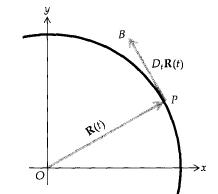
\includegraphics[width=0.4\linewidth]{figura-leithold1552.jpg}
  \caption{Esboço de um parte da Circunferência}\label{fig:1552}
\end{figure}

Para uma curva que descreve um movimento retilíneo uniforme, o vetor velocidade é constante. Em geral, o vetor velocidade é uma função vetorial
$v =\alpha'(t)$ que depende de $t$. A derivada $a=dv/dt =\alpha''(t)$ é chamada de vetor de aceleração da curva. Se a curva for $(x(t),\, y(t),\,
z(t))$, então o vetor de aceleração é
\begin{equation*}
\boxed{\quad \mathbf{a}=x''(t)e_{1}+y''(t)e_{2}+z''(t)e_{3} \quad}
\end{equation*}

\begin{exc}
Uma partícula se move de tal maneira que sua aceleração é constantemente igual a $-e_{3}$. Se a posição quando $t=0$ é $(0,\, 0,\, 1)$ e a
velocidade em $t=0$ é $e_{1}+e_{2}$, quando e onde a partícula cai abaixo do plano $z=0$? Descreva o caminho percorrido pela partícula.
\end{exc}

\solo
Seja $(x(t),\, y(t),\, z(t))$ a curva paramétrica traçada pela partícula, de modo que o vetor velocidade seja
\begin{equation*}
\alpha'(t)=x'(t)e_{1} + y'(t)e_{2}+z'(t)e_{3}.
\end{equation*}

Com a aceleração é  $\alpha''(t)=-e_{3}$, então $x''(t) = 0$, $y''(t) = 0$ e $z''(t)=-1$. Segue-se que $x'(t)$ e $y'(t)$ são funções constantes e
$z'(t)$ é uma função linear com inclinação $-1$.

Como $\alpha'(0)=e_{1}+e_{2}$, obtemos $\alpha'(t)=e_{1}+e_{2}-t\,e_{3}$.

Integrando novamente e usando a posição inicial $(0,\, 0,\, 1)$, encontramos que
\begin{equation*}
(x(t),\; y(t),\; z (t)) = \left(t,\; t,\; 1-(1/2)t^{2}\right).
\end{equation*}

A partícula cai abaixo do plano $z=0$ quando $1-(1/2)t^{2}=0$; ou seja, $t = 2$. Nesse momento, a posição é $\left(\sqrt{2},\, \sqrt{2},\,
0\right)$.

O caminho percorrido pela partícula é uma parábola no plano $y=x$ (ver Figura~\ref{fig:4-1-11-jerrold}) porque neste plano a equação dessa parábola é
descrita por $z=1-(1/2)x^{2}$. \hfill $\lozenge$

\begin{figure}[!h]
  \centering
  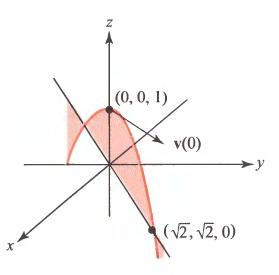
\includegraphics[width=0.45\linewidth]{graphics-4-1-11-jerrold.jpg}
  \caption{O caminho da parábola com posição inicial \((0,\, 0,\, 1)\), velocidade inicial \(e_{1}+e_{2}\) e a aceleração constante \(-e_{3}\) é uma parábola no plano \(y = x\).}
  \label{fig:4-1-11-jerrold}
\end{figure}


A imagem de um caminho $C^{1}$ não é necessariamente ``muito regular''; na verdade, ele pode ter curvas acentuadas ou mudanças de direção.

Por exemplo, o cicloide $\alpha(t) = (t-\sen t,\; 1-\cos t)$ mostrado na Figura~\ref{fig:2-4-6} tem cúspides em todos os pontos onde $\alpha$ toca o
eixo $x$ (isto é, quando $1-\cos t=0$, que acontece quando $t = 2\pi\,n$ com $n = 0, \pm 1, \ldots$).

Outro exemplo é o hipocicloide de nossas cúspides, $\alpha \colon [0,\; 2\pi] \to \mathbb{R}^{2}$, $t \mapsto (\cos^{3} t,\; \sen^{3} t)$, que possui
cúspides em quatro pontos (Figura~\ref{fig:4-1-2-jerrold}).
\begin{figure}[h!]
  \centering
  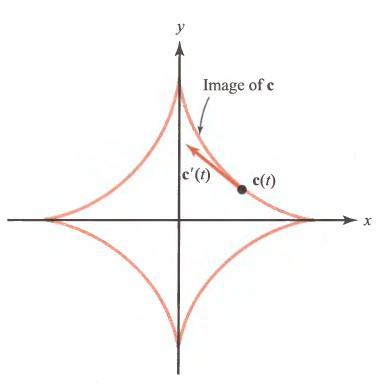
\includegraphics[width=0.45\linewidth]{graphic-4-1-2-jerrold.jpg}
  \caption{A imagem do caminho regular \(\alpha(t) = (\cos 3 t,\; \sen 3 t)\), um hipocicloide, não ``parece regular''.}
  \label{fig:4-1-2-jerrold}
\end{figure}

Em todos esses pontos, entretanto, $\alpha'(t) = 0$, e a reta tangente não está bem definida. Evidentemente, a direção de $\alpha'(t)$ pode mudar
abruptamente em pontos onde ele desacelera para o repouso.

Um caminho diferenciável $\alpha$ é considerado regular em $t=t_{0}$ se $\alpha'(t_{0}) \neq 0$. Se $\alpha'(t) \neq 0$ para todo $t$, dizemos que
$\alpha$ é um caminho regular. Nesse caso, a curva da imagem parece bem regular.

\begin{exc}
Uma partícula se move ao longo de um hipocicloide de acordo com as equações paramétricas,
\begin{equation*}
x = \cos^{3} t, \qquad  y = \sen^{3} t, \quad  a \leq  t \leq  b.
\end{equation*}

Quais são a velocidade e velocidade da partícula?
\end{exc}

\solo
O vetor velocidade da partícula é
\begin{equation*}
 v= \frac{d\, x}{dt}\,i+\frac{d\, y}{dt}\,j=-\left(3\sen t \cos^{2} t\right)\,i + \left(3 \cos t\sen^{2} t\right)\,j,
\end{equation*}
e sua velocidade escalar, o modulo do vetor velocidade, é
\begin{equation*}
s = |v| = \left(9\sen^{2} t \cos^{4} t + 9\cos^{2} t \sen^{4} t\right)^{1/2} = 3|\sen t||\cos t|.
\end{equation*}
e assim conclui-se o exercício. \hfill $\lozenge$

\noindent\textbf{Segunda Lei de Newton.}
Se uma partícula de massa $m$ se move em $\mathbb{R}^{3}$, a força $\mathbf{F}$ agindo sobre ela no ponto $\alpha(t)$ está relacionada à aceleração
pela segunda lei de Newton,
\begin{equation*}
\mathbf{F}(\alpha(t))=m\, \mathbf{a}(t).
\end{equation*}

Em particular, se nenhuma força atuar sobre uma partícula, então $\mathbf{a}(t)=0$, então $\alpha'(t)$ é constante e a partícula segue uma linha
reta.

\noindent\textbf{Aceleração e Segunda Lei de Newton.}
A aceleração de um percurso $\alpha(t)$ é
\begin{equation*}
  \mathbf{a}(t)=\alpha''(t).
\end{equation*}

Se $\mathbf{F}$ é a força atuante e $m$ é a massa da partícula, então
\begin{equation*}
  \mathbf{F}=m\, \mathbf{a}
\end{equation*}

No problema de determinar o caminho $\alpha(t)$ de uma partícula, a lei de Newton torna-se uma equação diferencial (ou seja, uma equação envolvendo
derivadas) para $\alpha(t)$.

\begin{exem}
Um planeta se movendo em torno do Sol (considerado como localizado na origem em $\mathbb{R}^{3}$) ao longo de um caminho $r(t)$ obedece à lei
\begin{equation*}
  m\, \mathbf{r}''=-\frac{G\, m\, M}{r^{3}}\, \mathbf{r}
\end{equation*}
onde $M$ é a massa do sol, $m$ a do planeta, $r = |r|$ e $G$ é a constante gravitacional.
\end{exem}

\solo
A relação usada na determinação da força,
\begin{equation*}
\mathbf{F} = -\frac{G\,m\, M}{r^{3}}\,\mathbf{r},
\end{equation*}
é chamada de lei da gravitação de Newton (ver Figura~\ref{fig:4-1-3-jerrold}).

\begin{figure}[h!]
  \centering
  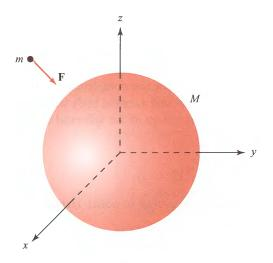
\includegraphics[width=0.45\linewidth]{graphics-4-1-3-Jerrold.jpg}
\caption{Uma massa \(M\) atrai uma massa \(m\) com uma força \(\mathbf{F}\) dada pela lei da gravitação de Newton:
\(\mathbf{F} = -G\,m\,M\, \mathbf{r}/r^{3}\).}
  \label{fig:4-1-3-jerrold}
\end{figure}


Não faremos um estudo geral de tais equações neste texto guia, mas nos contentaremos com o caso especial das órbitas circulares.
(Órbitas mais gerais -as seções cônicas- são discutidas e estudadas num suplemento mais avançado.)

\noindent\textbf{Órbitas Circulares.}
Considere uma partícula de massa $m$ movendo-se a velocidade constante $s$ em um caminho circular de raio $r_{0}$. Supondo que ele se mova no plano
$xy$, podemos suprimir a terceira componente e escrever
\begin{equation*}
\mathbf{r}(t)=\left(r_{0}\cos \dfrac{s\, t}{r_{0}}, \; r_{0}\sen \dfrac{s\,t}{r_{0}}\right),
\end{equation*}
uma vez que este é um círculo de raio $r_{0}$ e $|\mathbf{r}'(t)|=s$. Então
\begin{equation*}
\mathbf{a}(t)=\mathbf{r}''(t)=\left(-\frac{s^{2}}{r_{0}}\cos \frac{s\,t}{r_{0}}, \; -\frac{s^{2}}{r_{0}}\sen \frac{s\,t}{r_{0}} \right)= -\frac{s^{2}}{r_{0}^{2}}\, \mathbf{r}(t).
\end{equation*}

Assim, a aceleração está na direção oposta a $\mathbf{r}(t)$; isto é, ele é direcionado para o centro do círculo (veja a Figura~\ref{fig:4-1-4-jerrold}).

\begin{figure}[h!]
  \centering
  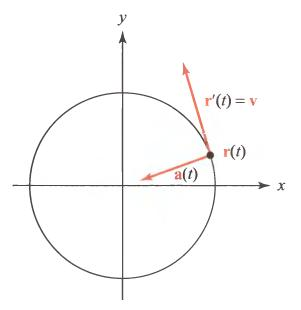
\includegraphics[width=0.35\linewidth]{graphics-4-1-4-jerrold.jpg}
  \caption{A posição, velocidade e aceleração de um partícula em movimento circular.}
  \label{fig:4-1-4-jerrold}
\end{figure}

Essa aceleração multiplicada pela massa da partícula é chamada de \textsf{força centrípeta}. Mesmo que a velocidade escalar é constante, a direção da
velocidade está mudando continuamente, a aceleração é uma taxa de mudança na velocidade escalar ou direção ou em ambas.

A lei de Newton nos ajuda a descobrir uma relação entre o raio da órbita de um corpo giratório e o período, ou seja, o tempo que leva para uma
revolução completa. Considere um satélite de massa $m$ movendo-se com velocidade escalar $s$ em torno de um corpo central de massa $M$ em uma órbita circular de raio $r_{0}$ (distância do centro do corpo central esférico). Pela segunda lei de Newton, $\mathbf{F}= m\, \mathbf{a}$, obtemos
\begin{equation*}
-\frac{s^{2}\, m}{r^{2}_{0}}\, \mathbf{r}(t)= -\dfrac{G\, m\, M}{r_{0}^{3}}\,\mathbf{r}(t).
\end{equation*}

Os comprimentos dos vetores em ambos os lados desta equação devem ser iguais. Por isso
\begin{equation*}
s^{2}= \frac{G\, M}{r_{0}}.
\end{equation*}

Se $T$ denota o período, então $s=2\pi\, r_{0}/T$, substituindo este valor por $s$ na equação acima e resolvendo para $T$, obtemos a seguinte lei,

\noindent\textbf{Lei de Kepler.}
\begin{equation*}
  T^{2}=r_{0}^{3}\,\dfrac{(2\pi)^{2}}{G\, M}.
\end{equation*}

Assim, o quadrado do período é proporcional ao cubo do raio.

Definimos dois conceitos básicos associados a um caminho ou percurso; sua velocidade e sua aceleração. Ambos envolvem cálculo \textsf{diferencial}. O
conceito básico do \textsf{comprimento de um caminho}, que envolve cálculo \textsf{integral}, será abordado na próxima seção.

\begin{exc}
Suponha que um satélite esteja em uma órbita circular em torno da Terra de forma que fique fixo no céu sobre um ponto no equador. Qual é o raio dessa órbita geossíncrona? (A massa da Terra é $5.98 \times 10^{24}$ quilogramas e $G=6.67 \times 10^{-11}$ no sistema de unidades metro-quilograma-segundo.)
\end{exc}

\solo
O período do satélite deve ser de $1$ dia, então $T = 60 \times 60 \times 24 = 86,400$ segundos. Da fórmula
\begin{equation*}
T^{2} = \dfrac{r^{3}_{0}\, (2\pi)^{2}}{G\,M}\quad \text{obtemos}\quad r^{3}_{0} = \dfrac{T^{2}\,G\, M}{(2\pi)^{2}}
\end{equation*}
e assim substituindo os valores dados,
\begin{align*}
r_{0}^{3} &= \frac{T^{2}\, G\, M}{(2\pi)^{2}}= \dfrac{(86,400)^{2}\times (6.67\times 10^{-11})\times (5.98\times 10^{24})}{(2\pi)^{2}}\\[2ex]
      & \approx 7.54 \times 10^{22}\, metros^{3}
\end{align*}

Assim, o raio da órbita é $r_{0} \approx 4.23 \times 10^{7}$ metros $= 42,300$ quilômetros $\approx 26,200$ milhas.


%
\section{Comprimento de Arco}
%
Na disciplina de Cálculo Diferencial obtivemos uma fórmula para encontrar o comprimento do arco de uma curva com uma equação da forma \(y=f(x)\). Este
é um tipo especial de curva porque o gráfico de uma função \(f\) não pode ser cruzado por uma linha vertical em mais de um ponto.

Qual é o comprimento de um percurso $\alpha(t)$? Já que a velocidade escalar $\|\alpha'(t)\|$ é a taxa de variação da distância percorrida em relação ao
tempo, a distância percorrida por um ponto que se move ao longo da curva é a integral da velocidade escalar em relação ao tempo no intervalo
$[t_{0},\; t_{1}]$ do tempo de viagem; ou seja, o comprimento do caminho, também chamado de comprimento do arco, é
\begin{equation*}
\int_{t_{0}}^{t_{1}}\|\alpha'(t)\|\, dt.
\end{equation*}

A seguir desenvolvemos um método para encontrar o comprimento do arco de alguns outros tipos de curvas. Seja \(\mathcal{C}\) a curva com equações
paramétricas
\begin{equation*}
x = f(t) \quad \text{e} \quad   y = g(t)
\end{equation*}
e suponha que \(f\) e \(g\) são contínuas no intervalo fechado \([a,\; b]\).

Desejamos atribuir um número \(L\) para representar o número de unidades para o comprimento do arco de \( \mathcal{C}\) de \(t = a\) a \(t = b\).

Seja \(P\)  uma partição do intervalo fechado \([a,\; b]\) formado pela divisão do intervalo em \(n\) subintervalos escolhendo \(n-1\) números entre \(a\) e \(b\).

Associado a cada número \(t_{i}\) está um ponto \(P_{i}(f(t_{i}),\; g(t_{i}))\) em \( \mathcal{C}\). De cada ponto \(P_{i-1}\) se desenha um segmento
de reta para o próximo ponto \(P_{i}\) (veja a Figura~\ref{fig:1561}).
\begin{figure}[!h]
  \centering
  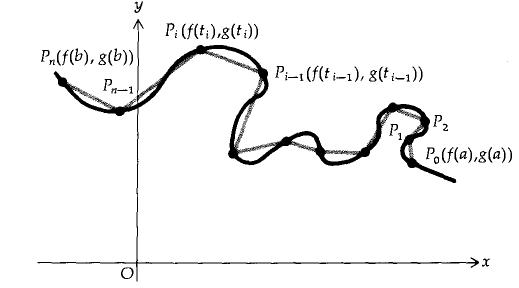
\includegraphics[width=0.6\linewidth]{figura-leithold1561}
  \caption{Noção Geométrica de Comprimento de Arco}\label{fig:1561}
\end{figure}

O número de unidades para comprimento do segmento de reta de \(P_{i-1}\) a \(P_{i}\) é denotado por \(\|\overline{P_{i-1}P_{i}}\|\). Da fórmula da distância temos
\begin{equation*}
\|\overline{P_{i-1}P_{i}}\|=\sqrt{[f(t_{i})-f(t_{i-1})]^{2}+[g(t_{i})-g(t_{i-1})]^{2}}
\end{equation*}

A soma dos números das unidades de comprimento dos $n$ segmentos de linha é
\begin{equation*}
  \sum_{i=1}^{n}\|\overline{P_{i-1}P_{i}}\|
\end{equation*}


\begin{defi}[Comprimento de Arco]\label{def:14-5-1}
	Suponha que a curva \( \mathcal{C}\) tenha equações paramétricas \(x = f (t)\) e \(y = g (t)\). Então, se existe um número \(L\) tendo a propriedade de que para qualquer \(\varepsilon > 0\) existe um \( \delta> 0\) tal que
	\begin{equation*}
		\left|\sum_{i=1}^{n}\|\overline{P_{i-1}P_{i}}\|- L \right| < \varepsilon
	\end{equation*}
	para cada partição \(P\) do intervalo \([a,\; b]\) para a qual a norma \(\|{P}\| <\delta\), escrevemos
	\begin{equation*}
		L=\lim_{|{P}| \to 0}\sum_{i=1}^{n}\|\overline{P_{i-1}P_{i}}\|
	\end{equation*}
	e \(L\) é denominado comprimento do arco da curva \(\mathcal{C}\) do ponto \((f(a),\; g (a))\) ao ponto
	\((f(b),\; g (b))\).
\end{defi}

O arco da curva é \textbf{retificável} se o limite na Definição~\ref{def:14-5-1} existir. Se \(f'\) e \(g'\) são contínuas em \([a,\; b]\), podemos
encontrar uma fórmula para calcular o limite \(L\).

Nossa noção intuitiva do \emph{comprimento do arco} de \(t = a\) até \(t = b\) nos leva a definir o número 
de unidades do comprimento do arco como o limite da soma quando a norma da partição \(|{P}|\) se aproxima de zero.  Uma outra forma mais analítica é a seguinte.

Seja \(\mathcal{C}\) uma curva descrita pela transformação \(\alpha\) de um intervalo fechado 
\([a,\; b]\) em \(\mathbb{R}^{n}\). Considere uma partição \(P =\{t_{i} \in E\vcentcolon i = 0,\ldots, 
k \}\) de \([a, \; b]\) onde \(a = t_{0} < t_{1} <\cdots < t_{k}= b\). Toda partição \(P\) de 
\([a,\; b]\) define uma poligonal  que consiste nos segmentos de reta de \(f(t_{0})\) a \(f(t_{1})\), de \(f(t_{1})\) a \(f(t_{2}),\ldots\), de \(f(t_{k-1})\) a \(f(t_{k})\). (Isso é ilustrado na Figura~\ref{fig:10-1} para o caso \(P=\{t_{0},\; t_{1},\; t_{2},\; t_{3},\; t_{4},\; t_{5}\}\).) Denotamos o  comprimento deste arco poligonal por \(L_{P}\), ou seja,
\begin{equation*}
L_{P} = \sum_{i\,=\, 1}^{n}\|\alpha(t_{i})- \alpha(t_{i-1})\|.
\end{equation*}
\begin{figure}[H]
\centering
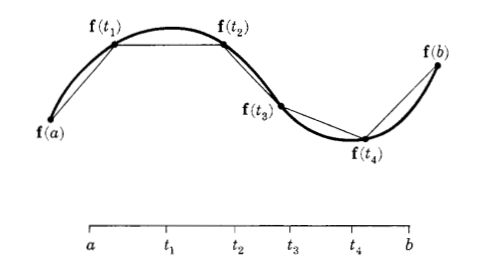
\includegraphics[width=0.5\textwidth]{partition-curve.jpg}
\caption{Um partição \(P\) do intervalo \(E\) com \(\boldsymbol{f}=\alpha\)}
\label{fig:10-1}
\end{figure}

Nossa ideia intuitiva de qual será o comprimento de \(\mathcal{C}\) nos diz que deveríamos ser
capazes de aproximar o comprimento de \(\mathcal{C}\) o máximo que desejarmos medindo os 
comprimentos \(L_{P}\) de arcos poligonais como os descritos. Além disso, como a distância ao 
longo de uma reta deve ser a  menor distância entre pontos, \(L_{P}\) ela deve ser menor que o 
comprimento de \(\mathcal{C}\), e se adicionarmos  pontos à partição \(P\), o comprimento do novo 
arco poligonal deve ser uma aproximação melhor do que  o original para o comprimento do arco 
\(\mathcal{C}\). Isso sugere a seguinte definição. Denotemos por \(\mathcal{P}\) o  conjunto de todas as partições do intervalo \([a,\; b]\).

\begin{defi}[Curva Retificável]
A curva \(\mathcal{C}\) descrita por uma transformação \(\alpha\) de \([a, \; b]\) é dita 
retificável se \(\{L_{P} \vcentcolon P \in \mathcal{P}\}\) tem um limite superior. Se \(\mathcal{C}\) é retificável, o comprimento \(L\) de \(\mathcal{C}\) é o 
supremo de \(\{L_{P} \vcentcolon P \in \mathcal{P}\}\); ou seja,
\begin{equation*}
 L = \sup \{L_{P} \vcentcolon P \in \mathcal{P}\}.
\end{equation*}
\end{defi}	

Este comprimento de uma curva está em conformidade com as ideias intuitivas mencionadas acima. 
Como \(L\) é um limite superior em \(\{L_{P} \vcentcolon P \in \mathcal{P}\}\), \(L\) é maior ou igual ao comprimento \(L_{P}\) de qualquer arco poligonal obtido tomando uma partição \(P\) de \([a,\; 
b]\). Além disso, para qualquer \(\varepsilon > 0\), existe 
uma partição \(P\) de \([a,\;b]\) tal que \(L-\varepsilon < L_{P} \leq  L\); caso contrário, 
\(L\) não seria o supremo (o menor limite superior) de \(\{Lp \vcentcolon P \in \mathcal{P}\}\).
	
Agora mostramos que, se obtivermos uma partição \(P_{2}\) de \([a,\; b]\) adicionando alguns 
pontos à partição \(P_{1}\) de \([a,\;b]\), então \(L_{P_{1}}\leq L_{P_{2}}\). Chamamos \(P_{2}\) 
de \texttt{refinamento} de \(P_{1}\).

\begin{lema}
Se \(P_{2}\) é um refinamento de \(P_{1}\), então 
\begin{equation*}
L_{P_{1}} \leq  L_{P_{2}}.
\end{equation*}
\end{lema}

\prova Este lema é uma consequência simples da desigualdade triangular. Seja \(\tau_{j}\) o primeiro ponto em \(P_{2}\) que não está em \(P_{1}\). Então, para algum \(i\), temos  \(t_{i-1} < \tau_{j} < t_{i}\) e
\begin{align*}
\|\alpha(t_{i})-\alpha(t_{i-1})\|&=\|\alpha(t_{i})-\alpha(\tau_{j}) +\alpha(\tau_{j})-\alpha(t_{i-1})\| \\[2ex]
& \leq \|\alpha(t_{i})-\alpha(\tau_{j})\|+ \|\alpha(\tau_{j})-\alpha(t_{i-1})\|
\end{align*}

Por um número finito de passos, podemos adicionar todos os pontos em \(P_{2}\) a \(P_{1}\) e obter \(L_{P_{1}} \leq  L_{P_{2}}\). \hfill \(\square\)

Se tivéssemos que usar a definição para calcular o comprimento de uma curva, nossa tarefa não 
seria fácil. No entanto, para a maioria das curvas de interesse, podemos encontrar o comprimento 
calculando uma integral.

Consideremos a curva \(\mathcal{C}\) descrita pela transformação \(\alpha\) de \([a,\; b]\) como 
a trajetória de uma partícula, onde $\alpha(t)$ é a posição da partícula no instante \(t\). 
Suponha que \(\alpha\) seja diferenciável em \([a,\; b]\). Então \(\alpha'(t)\) é a velocidade da 
partícula no instante \(t\) e \(|\alpha'(t)|\) é a ``velocidade'' da partícula no instante \(t\). 

Suponhamos que tomemos uma partição \(P\) de \([a,\; b]\) tal que a velocidade ``muda muito 
pouco'' em cada arco de \(f(t_{i-1})\) a \(f(t_{i})\); digamos que seja aproximadamente 
\(\alpha'(t^{\ast})\) neste arco, onde \(t^{\ast} \in [t_{i-1},\; t_{i}]\).

Então, usando a noção elementar de que distância é igual a ``velocidade'' multiplicada pelo 
tempo, o comprimento de \(\mathcal{C}\) é aproximadamente
\begin{equation*}
S_{P}=\sum_{i\,=\, 1}^{k}\|\alpha'(\tau^{\ast})\|(t_{i}-t_{i-1}).
\end{equation*}

Reconhecemos a \(S_{P}\) como a soma aproximada da integral \(\dst \int\|\alpha'(t)\|\,dt\), isto é,
\begin{equation*}
\int_{a}^{b}\|\alpha'(t)\|\,dt=\lim_{|P|\to 0}\, S_{P}
\end{equation*}
onde \(|P|\) denota a norma da partição \(P\),
\begin{equation*}
|P|=\max \{t_{i}-t_{i-1}\vcentcolon i = 1,\ldots, k\},
\end{equation*}
e esse limite significa,

Para \(\varepsilon >0\) existe um \(\delta =\delta(\varepsilon) >0\) tal que se
\begin{equation*}
|P| < \delta \quad \text{implica}\quad \left|S_{P}-\int_{a}^{b}\|\alpha'(t)\|\,dt\right| < \varepsilon
\end{equation*} 

Na discussão anterior, era necessário que a velocidade ``mudasse muito pouco'' no arco. Isso 
significa que precisamos que \(\alpha'\) seja contínua em \([a,\; b]\). Para funções do mundo 
real, sabemos que se uma função \(g\) é contínua em um intervalo fechado, então \(g\) é 
\texttt{uniformemente contínua} em \([a,\; b]\): isto é, para qualquer \(\varepsilon > 0\), 
existe um \(\delta=\delta(\varepsilon) > 0\) tal que
\begin{equation*}
\|g(x)-g(y)\| < \varepsilon\quad  \text{para todo}\quad  x,\; y \in [a,\; b]\quad  \text{sempre que}\quad  |x-y| < \delta.
\end{equation*}

Definimos \texttt{continuidade uniforme} para funções vetoriais da mesma forma e podemos provar 
que, se uma função vetorial é contínua em um intervalo fechado \([a,\; b]\), então ela é uniformemente  contínua  em \([a,\; b]\).

Agora estamos em condições de provar a fórmula integral para o comprimento de uma curva.


\begin{teo}[Curva Retificável]\label{thm:10-4}
Se \(\alpha\) tem uma derivada contínua em \([a,\; b]\), então a curva \(\mathcal{C}\) descrita por \(\alpha\) é retificável e
\begin{equation*}
L(\mathcal{C})=L=\int_{a}^{b}\|\alpha'(t)\|\,dt.
\end{equation*}
\end{teo}

\prova 
Na demonstração, consideramos \(\mathcal{C}\) como uma curva em \(\mathbb{R}^{3}\), embora o 
método possa ser aplicado independentemente da dimensão do espaço em que a curva é definida. Seja 
\(P = \{t_{0},\ldots,t_{k}\}\) uma partição de \([a,\; b]\). Pelo teorema do valor médio, 
\hfill \(\square\)

Formulamos um resultado particular do Teorema~\ref{thm:10-4} que fornece a fórmula do cálculo 
na forma de um teorema em \(\mathbb{R}^{2}\)
\begin{framed}
\begin{teo}\label{thm:15-6-3}
Seja  \( \mathcal{C}\) a curva com equações paramétricas \(x = f(t)\) e \(y = g(t)\), e suponha que \(f'\) e \(g'\)
sejam contínuas no intervalo fechado \([a,\, b]\). Então, o comprimento do arco \(L\)  da curva \(\mathcal{C}\) do
ponto \((f(a),\; g(a))\) ao ponto \((f(b),\; g(b))\) é determinado por
\begin{equation*}
\boxed{\quad  L = L(\mathcal{C})= \int_{a}^{b}\sqrt{[f'(t)]^{2}+[g'(t)]^{2}}\, dt \quad}
\end{equation*}
\end{teo}
\end{framed}


\begin{exc}
Seja \(\mathcal{C}\) a hélice cilíndrica descrita por
\begin{equation*}
\alpha(t) =\langle \cos t,\; \sen t, \; t/2\rangle. 
\end{equation*}
Determine o comprimento \(L\) do arco de \(\mathcal{C}\) de \((1,\; 0,\; 0)\) a 
\((-1,\; 0,\; \pi/2)\).
\end{exc}

\solo
Como \(\alpha(0) = \langle 1,\; 0,\; 0\rangle\) e \(\alpha(\pi) = \langle -1,\; 0,\; 
\pi/2\rangle\), aplicando a fórmula,
\begin{equation*}
L=L(\mathcal{C})=\int_{0}^{\pi}\|\alpha'(t)\|\,dt=\int_{0}^{\pi}\sqrt{\sen^{2}t+\cos^{2} t+1/4}\, dt = \int_{0}^{\pi}\dfrac{\sqrt{5}}{2}\,dt= \dfrac{\sqrt{5}}{2}\,\pi.
\end{equation*} 
 e isso concluí o exercício. \hfill \(\lozenge\) 
 
\begin{exc}
Determine o comprimento da curva \(\mathcal{C}\) descrita por
\begin{equation*}
\alpha(t) =\langle \cos t,\; \sen t \rangle, \quad  t \in [0,\; 4\pi].
\end{equation*}
\end{exc}

\solo 
A curva \(\mathcal{C}\) é o círculo unitário \(C(0,\; 1)\) percorrido duas vezes sob a 
transformação \(\alpha\) de \([0,\; 4\pi]\). Usando o Teorema~\ref{thm:10-4}, obtemos
\begin{equation*}
L=L(\mathcal{C})=\int_{0}^{4\pi}\sqrt{\sen^{2}t+\cos^{2} t}=\int_{0}^{4\pi}\,dt=
4\pi.
\end{equation*}
logo obtemos o resultado desejado. \hfill \(\lozenge\)


\begin{exc}
Encontre o comprimento do arco da curva com equações paramétricas
\begin{equation*}
x = t^{3} \quad \text{e} \quad y = 2\,t^{2},
\end{equation*}
em cada um dos seguintes casos: 
\begin{tasks}[label=(\alph*),item-indent=4em,label-width=4ex,ref=(\alph*)](2)
\task de \(t = 0\) a \(t = 1\);
\task de \(t = -2\) a \(t = 0\).
\end{tasks}
\end{exc}

\solo
Um esboço da curva é mostrado na Figura~\ref{fig:1562}.

\begin{figure}[H]
  \centering
  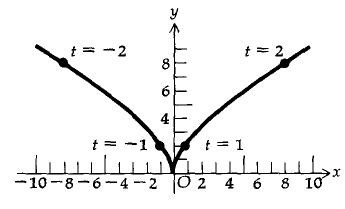
\includegraphics[width=3.0 in]{figura-leithold1562.jpg}
  \caption{Esboço da Curva}\label{fig:1562}
\end{figure}

(a) Fazendo \(x =f(t)\), derivando \(f'(t) = D_{t}x = 3t^{2}\); de forma semelhante \(y = g(t)\), derivando
\(g'(t) = D_{t}y = 4t\).

Portanto, a partir da fórmula dada no Teorema~\ref{thm:15-6-3}, se \(L\)  é o comprimento do arco da curva de \(t = 0\) a \(t = 1\),
\begin{align*}
  L & = \int_{0}^{1}\sqrt{9t^{4}+16t^{2}}\, dt=\int_{0}^{1}\sqrt{t^{2}}\sqrt{9t^{2}+16}\, dt \\[2ex]
    & = \int_{0}^{1}t\,\sqrt{9t^{2}+16}\, dt= \frac{1}{18}\frac{2}{3}\left(9t^{2}+16\right)^{3/2}\Bigg\vert_{t=0}^{1}\\[2ex]
    & =\frac{1}{27}\left[(25)^{3/2}+(16)^{3/2}\right]= \frac{1}{27}\left(125-64\right)=\frac{61}{27}
\end{align*}


(b) Se \(L\)  for o comprimento do arco da curva de \(t = -2\) a \(t = 0\), obtemos novamente usando a fórmula do Teorema~\ref{thm:15-6-3}
\begin{align*}
  L & = \int_{-2}^{0}\sqrt{9t^{4}+16t^{2}}\, dt=\int_{-2}^{0}\sqrt{t^{2}}\sqrt{9t^{2}+16}\, dt \\[2ex]
    & = \int_{-2}^{0}-t\,\sqrt{9t^{2}+16}\, dt=
-\frac{1}{18}\frac{2}{3}\left(9t^{2}+16\right)^{3/2}\Bigg\vert_{t=-2}^{0}\\[2ex]
&=-\frac{1}{27}\left[(16)^{3/2}-(52)^{3/2}\right]= \frac{1}{27}\left(104\sqrt{13}-64\right)\approx 11,5
\end{align*}

Utilizamos no item (a) a propriedade \(\sqrt{t^{2}}=t\) pois \( 0 \leq t \leq 1 \) e no item (b) o fato \( \sqrt{t^{2}}=-t\), pois \( -2 \leq t \leq 0\). \hfill \(\lozenge\)



Para a curva \(\mathcal{C}\) tendo como equações paramétricas \(x=f(t)\) e \(y=g(t)\), seja \(s\)  o comprimento do
arco de \( \mathcal{C}\)  do ponto \((f(t_{0}),\; g (t_{0}))\) ao ponto \((f(t),\; g (t))\), e vamos supor que \(s\)
seja crescente  à medida que \(t\) aumenta. Então \(s=s(t)\) é uma função de \(t\) e é dado por
\begin{equation*}
  s=s(t)=\int_{t_{0}}^{t}\sqrt{[f'(u)]^{2}+[g'(u)]^{2}}\,du
\end{equation*}

Pelo primeiro Teorema fundamental do Cálculo
\begin{equation}\label{eq:4-arc}
  \frac{ds}{dt}=\sqrt{[f'(t)]^{2}+[g'(t)]^{2}}
\end{equation}

A equação vetorial \(\alpha\) da curva \( \mathcal{C}\) e a sua derivada \(\alpha'\) são dadas por
\begin{equation}\label{eq:5-arc}
\alpha(t)=f(t)\, e_{1}+g(t)\, e_{2}\quad \text{e}\quad \alpha'(t)=f'(t)\, e_{1}+g'(t)\, e_{2}
\end{equation}
então o modulo do vetor velocidade é,
\begin{equation}\label{eq:6-arc}
  \|\alpha'(t)\|= \sqrt{[f'(t)]^{2}+[g'(t)]^{2}}.
\end{equation}

Substituindo o resultado dado em \eqref{eq:6-arc} num resultado prévio \eqref{eq:4-arc} obtemos uma nova fórmula
\begin{equation*}
  \boxed{\quad
  \|\alpha'(t)\|=\frac{ds}{dt}. \quad }
\end{equation*}

Da fórmula acima concluímos que se \(s\) for  o comprimento do arco da curva \(\mathcal{C}\) tendo a equação vetorial
\(\alpha\) medido entre algum ponto fixo ao ponto \((f(t),\; g(t))\) onde \(s\) é crescente à medida que \(t\)
aumenta, então a derivada de \(s\) em relação a \(t\) é a magnitude da derivada do vetor posição no ponto \((f(t),\;
g(t))\).

Se substituímos a relação \eqref{eq:6-arc} na fórmula proposta pelo Teorema~\ref{thm:15-6-3}, obtemos
\begin{equation*}
L=L(\mathcal{C}) = \int_{a}^{b} \|\alpha'(t)\|\, dt.
\end{equation*}

Então o Teorema~\ref{thm:15-6-3} pode ter seu formato vetorial proposto no seguinte teorema,

\begin{teo}\label{thm:15-6-4}
Seja a curva \(\mathcal{C}\) com equação vetorial \(\alpha(t) = f(t)\, e_{1} + g (t)\, e_{2}\), e suponha que \(f'\) e \(g'\) sejam contínuos no intervalo fechado \([a,\; b]\). Então, o comprimento do arco de \( \mathcal{C} \), traçado pelo ponto terminal da representação  posicional de \(\alpha(t)\) conforme \(t\) cresce a partir do extremo \(a\) para o extremo \(b\), é determinado por
\begin{equation*}
L = \int_{a}^{b} \|\alpha'(t)\|\, dt.
\end{equation*}
\end{teo}

\prova Tarefa para o leitor. \hfill \(\lozenge\)

\begin{exc}
Encontre o comprimento do arco traçado pelo ponto terminal da representação da posição de \(\alpha(t)\) quando \(t\) cresce de \(t=1\) para \(t=4\) se
\begin{equation*}
\alpha(t) = e^{t} \sen t \, i + e^{t} \cos t \, j
\end{equation*}
\end{exc}

\solo
Calculando o vetor velocidade,
\begin{equation*}
\alpha'(t)= \left(e^{t} \sen t + e^{t} \cos t\right)\, i + \left(e^{t} \cos t -e^{t} \sen t\right)\, j.
\end{equation*}

A seguir calculamos a velocidade escalar,
\begin{align*}
  \|\alpha'(t)\|^{2}&=\left(e^{t} \sen t + e^{t} \cos t\right)^{2} + \left(e^{t} \cos t -e^{t} \sen t\right)^{2}\\[2ex]
  &=e^{2t}\left(\sen^{2} t + 2\sen t \cos t + \cos^{2} t + \cos^{2} t - 2 \sen t \cos t + \sen^{2} t \right)\\[2ex]
  &= 2\,e^{2t}
\end{align*}

Aplicado a fórmula na forma vetorial
\begin{align*}
L&= \int_{1}^{4}\|\alpha'(t)\|\, dt=\int_{1}^{4}\sqrt{ 2\,e^{2t}}\, dt=\int_{1}^{4}\sqrt{2}\,e^{t}\, dt\\[2ex]
&= \sqrt{2}\,e^{t}\Bigg\vert_{t=1}^{4}=\sqrt{2}\,\left(e^{4}-e^{1}\right)=\sqrt{2}\,\left(e^{4}-e\right).
\end{align*}
 e isso concluí o exercício. \hfill \(\lozenge\)


Uma forma alternativa da fórmula dada pelo Teorema~\ref{thm:15-6-3} para o comprimento de um arco de uma curva \(\mathcal{C}\), tendo equações paramétricas \(x = f(t)\) e \(y = g(t)\), é obtida substituindo \(f'(t)\) por \(dx/ dt\) e \(g'(t)\) por \(dy/dt\), ou seja, pelo formato diferencial, o que fornece,
\begin{equation*}
L=\int_{a}^{b}\sqrt{\left( \frac{dx}{dt}\right)^{2}+\left(\frac{dy}{dt}\right)^{2}}\;dt
\end{equation*}


\begin{exc}
Calcular comprimento do arco do caminho
\begin{equation*}
\alpha(t) =\langle r \cos t,\; r \sen t \rangle \quad \text{para} \quad 0 \leq t \leq 2\pi.
\end{equation*}
\end{exc}

\solo
Aplicando a fórmula de comprimento de arco uma vez calculo as derivadas das funções componentes obtemos,
\begin{equation*}
L =\int_{0}^{2\pi}\sqrt{[-r \sen t]^{2} + [r\cos t]^{2}} \, dt = 2\pi r,
\end{equation*}
a circunferência de um círculo de raio \(r\).

Se tivéssemos permitido um domínio de \(0 \leq t \leq 4\pi\), teríamos obtido \(L=4\pi r\), porque o caminho
percorre a mesma circunferência duas vezes (ver Figura~\ref{fig:421})

\begin{figure}[H]
  \centering
  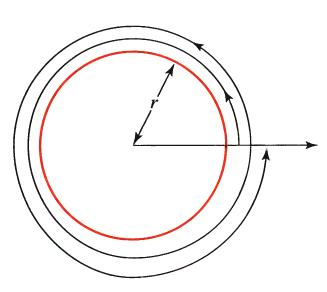
\includegraphics[width=0.3\linewidth]{figura-marsden421.jpg}
  \caption{O comprimento do arco de uma circunferência percorrido duas vezes é \(4\pi r\)}\label{fig:421}
\end{figure}

\bigskip
\noindent\textbf{Comprimento do Arco no Espaço.}
O comprimento da curva (caminho)  \(\alpha(t) =\langle x(t),\; y (t),\; z (t)\rangle \) para \(t_{0} \leq t \leq t_{1}\), é
\begin{equation*}
L=\int_{t_{0}}^{t_{1}}\sqrt{[x'(t)]^{2}+[y'(t)]^{2}+[z'(t)]^{2}}\, dt
\end{equation*}

Para curvas planas, omite-se o termo \(z'(t)\).


\begin{exc}
Encontre o comprimento do arco da curva representada por
 \begin{equation*}
 \alpha(t)=\langle \cos t,\; \sen t,\; t^{2} \rangle,\quad\text{para todo}\quad   0 \leq t  \leq \pi.
 \end{equation*}
\end{exc}

\solo
A função vetorial \(\alpha(t) = \langle \cos t,\; \sen t,\; t^{2}\rangle \) tem o vetor velocidade dado por
\(v =\alpha'(t)= \langle -\sen t, \; \cos t,\;  2t\rangle \). Posto que
\begin{equation*}
  \|\alpha(t)\|=\sqrt{\sen^{2} t+\cos^{2} t+4t^{2}}=\sqrt{1+4t^{2}}=2\sqrt{t^{2}+(1/2)^{2}}
\end{equation*}
o comprimento do arco é
\begin{equation*}
L=\int_{0}^{\pi}2\sqrt{t^{2}+(1/2)^{2}}\, dt.
\end{equation*}

Para calcular a integral usamos a seguinte formula
\begin{equation*}
\int \sqrt{x^{2}+a^{2}}\, dx =\frac{1}{2}\left[x\sqrt{x^{2}+a^{2}}+a^{2}\ln\left(x+\sqrt{x^{2}+a^{2}}  \right) \right]+C
\end{equation*}

Assim
\begin{align*}
  L & = 2\cdot\frac{1}{2}\left[t\sqrt{t^{2}+a^{2}}+(1/2)^{2}\ln \left(t+\sqrt{t^{2}+a^{2}} \right) \right]\Bigg\vert_{t=0}^{\pi} \\[2ex]
   & = \pi \sqrt{\pi^{2}+1/4}+\frac{1}{4}\ln \left(\pi+\sqrt{\pi^{2}+1/4}\right)-\frac{1}{4}\ln\left(\sqrt{{1}/{4}} \right)\\[2ex]
   & = \frac{\pi}{2}\sqrt{1+4\pi^{2}}+\frac{1}{4}\ln\left(2\pi +\sqrt{1+4\pi^{2}}\right) \approx 10,63.
\end{align*}

Para verificar nossa resposta, podemos notar que o caminho \(\alpha\) conecta os pontos \((1,\, 0,\, 0)\) e \((-1,\,
0,\, \pi^{2})\). A distância entre esses pontos é \(\sqrt{4 + \pi^{4}} \approx 10,06\), que é menor que \(10, \, 63\),
como deveria ser.

\bigskip
Se uma curva é composta por um número finito de peças, cada uma das quais \(C^{1}\) (com derivada limitada), calculamos o comprimento do arco adicionando os comprimentos das peças componentes. Essas curvas são chamadas de \(C^{1}\) por partes. Às vezes, apenas dizemos por ``regular por partes''.

\bigskip
\begin{exc}
Uma bola de bilhar em uma mesa quadrada segue o caminho $\alpha \colon [-1,\; 1] \to \mathbb{R}^{3}$ definido por $\alpha(t) =\langle x(t),\; y (t),\; z (t)\rangle =\langle |t|,\; |t-1/2|,\; 0\rangle $. Encontre a distância percorrida pela bola.
\end{exc}

\solo
Este percurso não é regular, porque $x(t) = |t|$ não é diferenciável em $0$, nem é $y(t) = |t-1/2|$ diferenciável em $1/2$. No entanto, se dividirmos o intervalo $[-1,\; 1]$ em partes ou subintervalos,
\begin{equation*}
[-1, \; 0], \quad  [0, \; 1/2], \quad  [1/2, \; 1],
\end{equation*}
vemos que $x(t)$ e $y(t)$ têm derivadas contínuas em cada um dos intervalos $[-1,\; 0]$, $[0,\; 1/2]$ e $[1/2,\; 1]$, (Veja a Figura~\ref{fig:4-2-2-jerrold})

Em $[-1,\; 0]$, $x(t) =-t$, $y(t) =-t + 1/2$ e $z (t) = 0$, então $\|\alpha'(t)\|=\sqrt{2}$. Portanto, o comprimento do arco de $\alpha$ entre $-1$ e
$0$ é dado pela integral definida,
\begin{equation*}
\int_{-1}^{0} \|\alpha'(t)\|\, dt=\int_{-1}^{0} \sqrt{2}\, dt = \sqrt{2}.
\end{equation*}

Da mesma forma, em $[0,\; 1/2]$, $x(t) = t$, $y(t)=-t + 1/2$, $z(t)=0$, e novamente $|\alpha'(t)|=\sqrt{2}$, de modo que o comprimento do arco de
$\alpha$ entre $0$ e $1/2$ é,
\begin{equation*}
\int_{0}^{1/2} \|\alpha'(t)\|\, dt=\int_{0}^{1/2} \sqrt{2}\, dt = \dfrac{1}{2}\sqrt{2}.
\end{equation*}

Finalmente, em $[1/2,\; 1]$ temos $x(t) = t$, $y(t)=t-1/2$, $z(t)=0$, então $|\alpha'(t)|=\sqrt{2}$, de modo que o comprimento do arco de $\alpha$ entre
$1/2$ e $1$ é,
\begin{equation*}
\int_{1/2}^{1} \|\alpha'(t)\|\, dt=\int_{1/2}^{1} \sqrt{2}\, dt = \dfrac{1}{2}\sqrt{2}.
\end{equation*}

Assim, o comprimento total do arco de $\alpha$,
\begin{equation*}
\int_{-1}^{1}\|\alpha'(t)\|\, dt=\int_{-1}^{0}\sqrt{2}\, dt+\int_{0}^{1/2}\sqrt{2}\, dt + \int_{1/2}^{1}\sqrt{2}\, dt =2\sqrt{2},
\end{equation*}
é o resultado que procuramos. \hfill $\lozenge$

\begin{figure}[H]
  \centering
  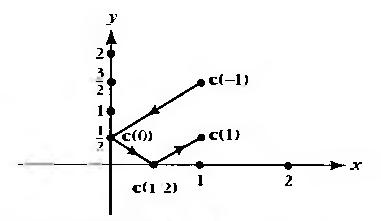
\includegraphics[width=0.6\linewidth]{graphics-4-2-2-jerrold.jpg}
  \caption{Percurso regular por partes}
  \label{fig:4-2-2-jerrold}
\end{figure}

\bigskip
\begin{exc}
Considere o ponto com função de posição
\begin{equation*}
\alpha(t) =\langle t-\sen t,\; 1-\cos t \rangle,
\end{equation*}
que traça o cicloide (veja a Figura~\ref{fig:2-4-6}). Encontre o vetor velocidade, a velocidade escalar e o comprimento de um arco.
\end{exc}

\solo
O vetor velocidade é \(\alpha'(t) =\langle 1- \cos t,\; \sen t\rangle \), então a velocidade escalar do ponto \(\alpha(t)\) é
\begin{equation*}
\|\alpha'(t)\| = \sqrt{(1-\cos t)^{2} + \sen^{2} t} = \sqrt{2 - 2 \cos t}.
\end{equation*}

Consequentemente, \(\alpha(t)\) se move a uma velocidade variável, embora o círculo role a uma velocidade constante.
Além disso, a velocidade de \(\alpha(t)\) é zero quando \(t\) é um múltiplo inteiro de \(2\pi\). Com esses valores de
\(t\), a coordenada \(y\) do ponto \(\alpha(t)\) é zero e, portanto, o ponto está no eixo \(x\). O comprimento do
arco de um ciclo é
\begin{align*}
  L& =\int_{0}^{2\pi}\sqrt{2-2\cos t}\,dt=2\int_{0}^{2\pi}\sqrt{\frac{1-\cos t}{2}}\, dt \\[2ex]
   &= 2\int_{0}^{2\pi}\sen \frac{t}{2}\; dt=4\left(-\cos \frac{t}{2}\right)\Bigg\vert_{t=0}^{2\pi}=8
\end{align*}

Utilizamos a seguintes identidades trigonométricas
\begin{equation*}
1-\cos t=2\sen^{2} \frac{t}{2}\quad \text{e} \quad  \sen \frac{t}{2} \geq 0 \quad  \text{sobre}\quad [0,\; 2\pi]
\end{equation*}

\begin{figure}[H]
  \centering
  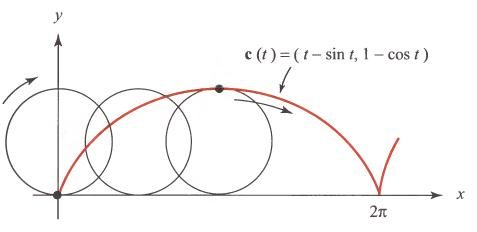
\includegraphics[width=0.6\linewidth]{figura-marsden246.jpg}
  \caption{A curva traçada por um ponto que se move na borda de um círculo rolante é chamada de cicloide.}
  \label{fig:2-4-6}
\end{figure}

\bigskip
\noindent\textbf{O Diferencial do Comprimento do Arco.}
A fórmula do comprimento do arco sugere que se introduza a seguinte notação, que será útil em nossa discussão sobre integrais de linha.

Um \emph{deslocamento infinitesimal} de uma partícula seguindo um caminho
\begin{equation*}
\alpha(t) = x(t)\,e_{1} + y(t)\,e_{2} + z(t)\, e_{3}
\end{equation*}
é
\begin{equation*}
ds=dx\,e_{1}+dy\,e_{2}+dz\,e_{3}=\left(\frac{dx}{dt}e_{1}+\frac{dy}{dt}e_{2}+\frac{dz}{dt}e_{3} \right)\,dt
\end{equation*}
e seu comprimento
\begin{equation*}
\|ds\|=\sqrt{dx^{2}+dy^{2}+dz^{2}}=\sqrt{\left( \frac{dx}{dt}\right)^{2}+\left(\frac{dy}{dt}
\right)^{2}+\left(\frac{dz}{dt} \right)^{2}}\,dt
\end{equation*}
é o diferencial do comprimento do arco. Veja a Figura~\ref{fig:4-2-3}.

\begin{figure}[H]
  \centering
  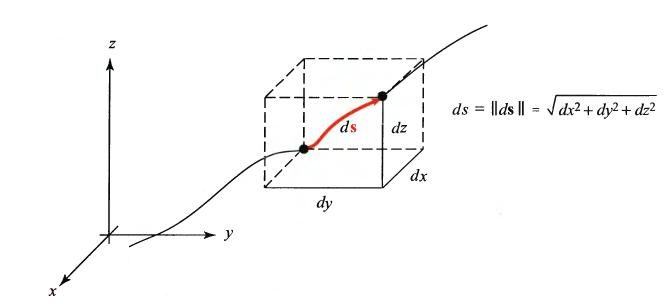
\includegraphics[width=0.7\linewidth]{figura-marsden423.jpg}
  \caption{Diferencial do comprimento do arco.}\label{fig:4-2-3}
\end{figure}

Essas fórmulas nos ajudam a lembrar a fórmula do comprimento do arco como
\begin{equation*}
\boxed{\quad   \text{comprimento do arco}\; = \; \int_{t_{0}}^{t_{1}}\,\|ds\|. \quad}
\end{equation*}

Como fizemos antes com conceitos geométricos como comprimento e ângulo, podemos estender a noção de comprimento do arco para funções vetoriais no espaço \(n\)-dimensional.

\bigskip
\noindent\textbf{Comprimento de Arco n-dimensional.}
Considere \(\alpha\colon [t_{0},\; t_{1}] \to \mathbb{R}^{n}\) uma função vetorial. Seu comprimento é definido
\begin{equation*}
  L=\int_{t_{0}}^{t_{1}}\|\alpha'(t)\|\,dt
\end{equation*}

O integrando é a raiz quadrada da soma dos quadrados das funções coordenadas de \(\alpha'(t)\); se
\begin{equation*}
\alpha(t) = \left\langle x_{1}(t),\;x_{2}(t), \ldots, x_{n}(t) \right\rangle,
\end{equation*}
então
\begin{equation*}
L=\int_{t_{0}}^{t_{1}}\sqrt{[x'_{1}(t)]^{2}+[x'_{2}(t)]^{2}+\cdots+[x'_{n}(t)]^{2}}\;dt
\end{equation*}

\begin{exc}
Encontre o comprimento do caminho
\begin{equation*}
\alpha(t) = \left\langle\cos t,\; \sen t,\; \cos 2t,\; \sen 2t\right\rangle\quad \text{em}\quad \mathbb{R}^{4}
\end{equation*}
definido no intervalo de \(0\) a \(\pi\).
\end{exc}

\solo
Temos a derivada da função vetorial,  \(\alpha'(t) =\langle -\sen t,\; \cos t,\; -2 \sen 2t, \; 2 \cos 2t \rangle\), e assim
\begin{equation*}
\|\alpha'(t)\| = \sqrt{\sen^{2} t + \cos^{2} t + 4 \sen^{2} 2t + 4 \cos^{2} 2t} =  \sqrt{1+4} = \sqrt{5},
\end{equation*}
uma constante, então
\begin{equation*}
\int_{0}^{\pi}\sqrt{5} \, dt = \sqrt{5}\pi,
\end{equation*}
é o comprimento do caminho dado. \hfill $\lozenge$

\bigskip
É comum introduzir a função de comprimento de arco \(s(t)\) associada a um caminho \(\alpha(t)\) definido por
\begin{equation*}
s(t) =\int_{a}^{t} \|\alpha'(u)\|\, du,
\end{equation*}
de modo que (pelo teorema fundamental do cálculo)
\begin{equation*}
s'(t) = \|\alpha'(t)\|,
\end{equation*}
integrando de forma definida e usando a definição da função $s(t)$,
\begin{equation*}
  \int_{a}^{b}s'(t)\,dt=s(b)-s(a) = s(b).
\end{equation*}

\begin{exc}
Considere o gráfico de uma função de uma variável \(y = f (x) \) para \(x\) no intervalo \([a, \;  b]\).  Encontre  seu comprimento de arco.
\end{exc}

\solo
Podemos considerá-la uma curva parametrizada por \(t = x\), ou seja,
\begin{equation*}
\alpha (x) = \langle x, \; f (x)\rangle \quad \text{para} \quad  x \in  [a,\;  b].
\end{equation*}

Aplicando a fórmula  do comprimento do arco  encontramos,
\begin{equation*}
 L= \int_{a}^{b}\|\alpha'(x)\|\, dx =\int_{a}^{b}\sqrt{1 +[f'(x)]^{2}]}\, dx
\end{equation*}
o que concorda com a fórmula para o comprimento de um gráfico do cálculo de uma variável.


%%%
\subsection{Derivadas de um vetor em relação ao comprimento do arco de uma Curva}
%%%%
Considere uma curva \(L\) no espaço. Nela, escolha um ponto \(M_{0}\) como origem e também uma 
direção ao longo de \(L\) que será considerada positiva. Como parâmetro, tome o comprimento de 
arco \(s\) calculado a partir de \(M_{0}\) da curva, veja a Figura~\ref{fig:3-2-9}. Então, o raio  vetor  de um ponto 
\(M\) da curva é
\begin{equation*}
\alpha= \alpha(s).
\end{equation*}

Com essa escolha de parâmetro,
\begin{equation*}
\dfrac{d\alpha}{ds}=\tau
\end{equation*}
onde \(\tau\) é um vetor unitário direcionado ao longo da tangente à curva \(L\) na direção dos valores crescentes do parâmetro \(s\).
\begin{figure}[H]
\centering
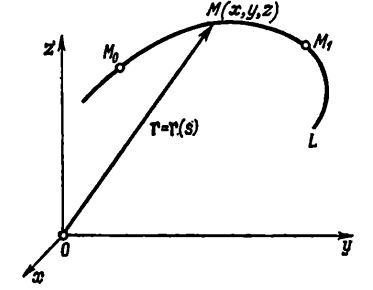
\includegraphics[width=0.5\textwidth]{comprimento-curva-parametro.jpg}
\caption{O raio vetor \(\alpha\) de um ponto \(M\) da curva \(L\)}
\label{fig:3-2-9}
\end{figure}


\subsection{A curvatura de uma Curva}

Se o vetor \(\alpha\) é dado pelas coordenadas
\begin{equation*}
	\alpha = x\,e_{1} + y\,e_{2} + z\, e_{3},
\end{equation*}
então
\begin{equation*}
	\tau = \dfrac{dx}{ds}\, e_{1} + \dfrac{dy}{ds}\, e_{2} + \dfrac{dz}{ds}\,e_{3}
\end{equation*}
e
\begin{equation*}
	\sqrt{\left(\dfrac{dx}{ds}\right)^{2}+\left(\dfrac{dy}{ds}\right)^{2}+\left(\dfrac{dz}{ds}\right)^{2}}=1.
\end{equation*}

Como \(\|\tau\| = 1\), o vetor \(d\tau/ds\) é \texttt{ortogonal} ao vetor \(\tau\).

O módulo do vetor \(d\tau/ds\) é
\begin{equation*}
	\left\|\dfrac{d\tau}{ds}\right\| = K.
\end{equation*}

Aqui, \(K\) é a curvatura da curva \(L\) no ponto \(M\).

A reta que tem a direção do vetor \(d\tau/ds\) e passa pelo ponto \(M\) da curva é denominada 
\texttt{normal principal} da curva no ponto \(M\).

Denotando o vetor unitário dessa direção por \(\boldsymbol{\nu}\), temos
\begin{equation}\label{eq:3-2-1}
	\dfrac{d\tau}{ds}= K\, \boldsymbol{\nu}.
\end{equation}

O inverso da curvatura de uma curva em um determinado ponto
é chamado de \texttt{raio de curvatura} da curva naquele ponto
e é denotado por \(R\),
\begin{equation*}
R=\dfrac{1}{K}.
\end{equation*}

Assim, a fórmula \eqref{eq:3-2-1} pode ser reescrita como
\begin{equation*}
\dfrac{d^{2}\alpha}{ds^{2}}=\dfrac{d\tau}{ds}=\dfrac{\boldsymbol{\nu}}{R}.
\end{equation*}

A partir disso,
\begin{equation*}
K=\dfrac{1}{R}=\left\|\dfrac{d^{2}\alpha}{ds^{2}}\right\|
\end{equation*}
ou
\begin{equation}\label{eq:3-2-2}
K=\dfrac{1}{R}=\sqrt{\left(\dfrac{d^{2}x}{ds^{2}}\right)^{2}+\left(\dfrac{d^{2}y}{ds^{2}}\right)^{2}+\left(\dfrac{d^{2}z}{ds^{2}}\right)^{2}}
\end{equation}

Usando a fórmula \eqref{eq:3-2-2}, podemos calcular a curvatura de uma curva em qualquer
ponto se a curva for especificada por equações paramétricas em
que o parâmetro é o comprimento do arco \(s\).

No caso particular de uma curva plana, um círculo de raio \(a\),
\begin{equation*}
\left\{
\begin{array}{cl}
x = & a \cos \dfrac{s}{a}\\[2ex]
y =& a \sen \dfrac{s}{a}
\end{array}
\right.
\end{equation*}
temos
\begin{equation*}
\dfrac{d^{2}x}{ds^{2}}=-\dfrac{1}{a}\cos\left(\dfrac{s}{a}\right), \quad
\dfrac{d^{2}y}{ds^{2}}=-\dfrac{1}{a}\sen \left(\dfrac{s}{a}\right)
\end{equation*}
e a fórmula \eqref{eq:3-2-2} produz
\begin{equation*}
K=\dfrac{1}{R}=\sqrt{\dfrac{1}{a^{2}}\cos^{2} \frac{s}{a}+ 
\dfrac{1}{a^{2}}\sen^{2} \frac{s}{a}}= \dfrac{1}{a}.
\end{equation*}

Isso significa que a curvatura de um círculo de raio \(a\) é constante e é igual ao inverso do 
raio do círculo.

Se a curva \(L\) for dada pela equação vetorial paramétrica \(\alpha=\alpha(t)\), onde o parâmetro \(t\) é arbitrário, então
\begin{equation}\label{eq:3-2-3}
K = \dfrac{1}{R}=\dfrac{\left\|\dfrac{d\alpha}{dt}\times \dfrac{d^{2}\alpha}{dt^{2}} \right\|}{\left\|\dfrac{d\alpha}{dt}\right\|^{3}}
\end{equation}

A fórmula \eqref{eq:3-2-3} permite calcular a curvatura da curva em qualquer ponto, desde que tenhamos uma especificação paramétrica arbitrária dessa curva.

\begin{exc}
Calcule a curvatura da curva helicoidal
\begin{equation*}
\alpha(t) = a\cos t\,e_{1} + a\sen t\, e_{2} + ht\, e_{3}.
\end{equation*}
\end{exc}

\solo Como a primeira e segunda derivada são dadas por,
\begin{align*}
\dfrac{d\alpha}{dt}&=  -a\sen t\,e_{1} + a\cos t\, e_{2} + h\, e_{3}.\\[2ex]
\dfrac{d^{2}\alpha}{dt^{2}}&= -a\cos t\,e_{1} - a\sen t\, e_{2} + 0\, e_{3}.
\end{align*}
e seu produto vetorial
\begin{equation*}
\dfrac{d\alpha}{dt}\times \dfrac{d^{2}\alpha}{dt^{2}}=
\begin{vmatrix}
e_{1} & e_{2} & e_{3}\\
-a\sen t& a\cos t & h\\
-a\cos t& -a\sen t & 0
\end{vmatrix}=ah\sen t\, e_{1}-ah\cos t\,e_{2}+a^{2}\,e_{3}.
\end{equation*}

Consequentemente,
\begin{equation*}
\left\|\dfrac{d\alpha}{dt}\times \dfrac{d^{2}\alpha}{dt^{2}}\right\|=a\sqrt{a^{2}+h^{2}} \quad \text{e}\quad 
\left\|\dfrac{d\alpha}{dt}\right\|= \sqrt{a^{2}+h^{2}}. 
\end{equation*}

Em virtude da fórmula \eqref{eq:3-2-3},
\begin{equation*}
K=\dfrac{1}{R}=\dfrac{a}{a^{2}+h^{2}}
\end{equation*}
ou
\begin{equation*}
R= \dfrac{a^{2}+h^{2}}{a}=\text{constante}.
\end{equation*}

Assim, uma curva helicoidal tem um raio de curvatura constante. \hfill \(\lozenge\)

%%%%
\section*{Exercícios Propostos}
%%%%
\begin{enumerate}[label=(\arabic*),ref=(\arabic*)]
\item Encontre o raio de curvatura de cada uma das curvas fornecidas.
\begin{enumerate}
\item \(\alpha =\ln \cos t\, e_{1} +\ln \sen t\, e_{2} +\sqrt{2t}\, e_{3}.\)
\item \(\alpha =t^{2}\,e_{1} + 2t^{3}\,e_{2}\)	
\item  \(\alpha =3t^{2}\, e_{1}+(3t-t^{3})\,e_{2}+2\, e_{3}\)\quad  para\quad  \(t=1\).
\item \(\alpha = a (\cos t + t \sen t)\,e_{1} + a (\sen t - t \cos t)\, e_{3}\)\quad  para \quad  \(t=\pi/2\).
\item \(\alpha =a \cosh t\, e_{1} +a\senh t\,e_{2} + at\,e_{3}\) \quad  em qualquer ponto \quad \(t\).
\end{enumerate}	
\end{enumerate}


%%
\chapter{Funções Reais de Várias Variáveis}
%%
%%%%%%%%%
\section{Derivadas Direcionais e Vetor Gradiente}
%%%%%
Sabemos pela da regra da cadeia que se \(f(x,\; y)\) é diferenciável, então a taxa com que \(f\) varia em
relação a \(t\) ao longo de uma curva diferenciável \(x=g(t)\), \(y = h(t)\) é,
\begin{equation*}
	\frac{df}{dt}=\frac{df}{dx}\,\frac{dx}{dt}+\frac{df}{dy}\,\frac{dy}{dt}
\end{equation*}

Em qualquer ponto \(P_{0}= (x_{0},\;y_{0}) = P_{0}(g(t_{0}),\; h(t_{0}))\), essa equação fornece a taxa de variação de \(f\) em relação a \(t\) e, portanto, depende, entre outras coisas, do sentido do movimento ao longo da curva.

Essa observação e particularmente importante quando a curva é uma reta e \(t\) é o parâmetro de comprimento de arco
ao longo da reta medida de \(P_{0}\) na direção de dado vetor unitário, ou versor, \(u\), pois, nesse caso, \(df/dt\) é a taxa de variação de \(f\) em relação à distância em seu domínio na direção de \(u\). Variando \(u\), encontramos as taxas com que \(f\) varia em relação à distancia quando nos movemos por \(P_{0}\) em direções diferentes. Nesta seção mostremos uma formula para calculá-las e a partir disto podemos encontra fórmulas de equações de planos tangentes e retas normais a superfície $S$ no espaço.

%
\subsection{Derivadas Direcionais no Plano}
%

A seguir desenvolveremos  essa ideia com maior precisão. Suponha que a função \(f(x,\; y)\) seja definida em uma
região \(\Omega\) no plano \(xy\), que \(P_{0}=(x_{0},\; y_{0})\), seja um ponto em \(\Omega\) e que \(u = u_{1}e_{1}
+ u_{2}e_{2}\)  seja um vetor unitário. Então as equações
\begin{equation*}
	x = x_{0}+su_{1}, \quad \text{e}\quad y=y_{0}+su_{2}
\end{equation*}
parametrizam a reta que passa por \(P_{0}\) paralelamente a \(u\). Se o parâmetro \(s\) mede o comprimento de arco de
\(P_{0}\) na direção de \(u\), encontramos a taxa de variação de \(f\) em \(P_{0}\) e na direção de \(u\) calculando
\(df/ds\) em \(P_{0}\).  Veja a Figura~\ref{fig:14-26-thomas}

\begin{defi}[Derivada Direcional]
	A derivada de \(f\)em \(P_{0}(x_{0},\; y_{0})\) na direção do versor \(u = u_{1}e_{1} + u_{2}e_{2}\) é o número
	\begin{equation*}
		(D_{u}f)_{P_{0}}=\left(\frac{df}{ds}\right)_{u,\, P_{0}}=\lim_{s \to 0}
		\dfrac{f(x_{0}+su_{1}, \; y_{0}+su_{2})-f(x_{0},\; y_{0})}{s}
	\end{equation*}
	desde que o limite exista.
\end{defi}

A derivada direcional é denotada também pelo símbolo,
\begin{equation*}
	\left(D_{u}f \right)_{P_{0}} \quad \text{``Derivada de \(f\) em \(P_{0}\) na direção de \(u\)'' }
\end{equation*}

\begin{figure}[!h]
	\centering
	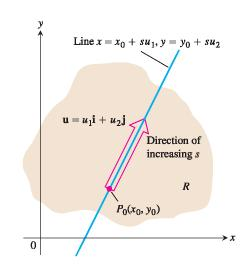
\includegraphics[width=0.4\linewidth]{graphics-14-26-thomas.jpg}
	\caption{A taxa de variação de \(f\) em a direção de \(u\) no ponto \(P_{0}\) é a taxa com que \(f\) varia ao longo desta reta em \(P_{0}\).}
	\label{fig:14-26-thomas}
\end{figure}

A seguir resolveremos um exercício utilizando a definição de derivada direcional,
\begin{exc}
	Encontre a derivada da função,
	\begin{equation*}
		f(x,\; y)=x^{2}+xy
	\end{equation*}
	em \(P_{0}(1,\; 2)\) na direção do vetor unitário \(u = (1/\sqrt{2})\,e_{1}+(1/\sqrt{2})\,e_{2}\)
\end{exc}

\textbf{Solução.}
Calculando o quociente da definição,
\begin{align*}
	\dfrac{f(x_{0}+su_{1}, \; y_{0}+su_{2})-f(x_{0},\; y_{0})}{s} &= \frac{f\left(1+s\cdot \dfrac{1}{\sqrt{2}},\;
		2+s\cdot \dfrac{1}{\sqrt{2}} \right)-f(1,\; 2)}{s} \\
	&=\dfrac{(1+s/\sqrt{2})^{2}+(1+s/\sqrt{2})(2+s/\sqrt{2}))-(1^{2}+1\cdot 2)}{s}\\
	&=\dfrac{\left(1+\dfrac{2s}{\sqrt{2}}+\dfrac{s^{2}}{2}\right)+\left(2+\dfrac{3s}{\sqrt{2}}+\dfrac{s^{2}}{2}\right)-3}{s}\\
	&=\dfrac{s^{2}+\dfrac{5s}{\sqrt{2}}}{s}
\end{align*}

Aplicando limite quando \(s \to 0\) no calculo anterior
\begin{equation*}
	\lim_{s \to 0} \dfrac{s^{2}+\dfrac{5s}{\sqrt{2}}}{s}=\lim_{s \to 0}\left(\dfrac{5}{\sqrt{2}}+s \right)=
	=\left(\frac{5}{\sqrt{2}}+0\right)=\frac{5}{\sqrt{2}}
\end{equation*}

A taxa de variação de \(f(x,\; y) = x^{2} + xy\) em \(P_{0}(1,\; 2)\) na direção de \(u\) é dada por \(D_{u}f((1,\;
2))= 5/\sqrt{2}\).



%
\subsection{Interpretação Geométrica}
%
A equação $z = f(x,\, y)$ representa uma superfície $S$ no espaço. Se $z_{0} = f(x_{0},\, y_{0})$, então o ponto $P(x_{0},\, y_{0},\, z_{0})$ está em
$S$. O plano vertical que passa por $P$ e $P_{0}(x_{0},\, y_{0})$ paralelo a $u$ intercepta $S$ em uma curva $\mathcal{C}$ (Veja
Figura~\ref{fig:14-27-thomas}). A taxa de variação de $f$ na direção de $u$ é a inclinação da tangente a $\mathcal{C}$ em $P$ no sistema destro
formado pelos vetores $u$ e $k$.

Quando $u=i$, a derivada direcional em $P_{0}$ é $\partial_{x}f$ calculada em $(x_{0},\, y_{0})$. Quando $u=j$, a derivada direcional em $P_{0}$ é
$\partial_{y}f$ avaliada em $(x_{0},\, y_{0})$. A derivada direcional generaliza as duas derivadas parciais. Agora podemos pedir a taxa de variação de
$f$ em qualquer direção $u$, não apenas as direções dos versores $i$ e $j$.

\begin{figure}[!h]
	\centering
	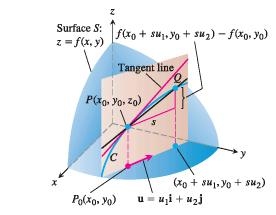
\includegraphics[width=0.65\linewidth]{graphics-14-27-thomas.jpg}
	\caption{A inclinação da curva \(\mathcal{C}\) em \(P_{0}\) é \(\dst{\lim_{p\to Q}}\text{coeficiente angular\,(PQ)}\); esta é a derivada direcional
		\(\left(\dfrac{df}{ds} \right)_{u,\; P_{0}} = (D_{u}f)_{P_{0}}\)}
	\label{fig:14-27-thomas}
\end{figure}

%
\subsection{Cálculos com Derivadas Direcionais}
%

Podemos formular uma segunda definição equivalente,
\begin{defi}[Derivada Direcional]
	Se \(f (x,\; y)\) é uma função de \(x\) e \(y\), e se \(u = u_{1}\,i + u_{2}\, j\) é um vetor unitário, então a derivada direcional de \(f\) na direção de \(u\) em \((x_{0},\; y_{0})\) é denotada por \(D_{u}f (x_{0}, \; y_{0})\) e é definido por
	\begin{equation}\label{eq:2-def}
		D_{u}f(x_{0}, \; y_{0}) =\frac{d}{ds}\bigl[f(x_{0} + su_{1},\;  y_{0} + su_{2})  \bigr]\bigg\vert_{s=0}
	\end{equation}
	desde que esta derivada exista.
\end{defi}


\begin{exc}
	Seja \(f(x,\; y) = xy\). Encontre e interprete \(D_{u}f (1, \; 2) \) para o vetor unitário
	\begin{equation*}
		u = \frac{\sqrt{3}}{2}\, i + \frac{1}{2}\, j.
	\end{equation*}
\end{exc}

\textbf{Solução.}
Conclui-se  a partir  da equação \eqref{eq:2-def} que
\begin{equation*}
	D_{u}f(1,\; 2) =\frac{d}{ds}\left[ f\left(1+\frac{\sqrt{3}}{2}s, \; 2+\frac{1}{2}s \right) \right]\Bigg\vert_{s=0}.
\end{equation*}

Posto que,
\begin{equation*}
	f\left(1+\frac{\sqrt{3}}{2}s, \; 2+\frac{1}{2}s \right)=\left(1+\frac{\sqrt{3}}{2}s \right) \left( 2+\frac{1}{2}s\right)
	=\frac{\sqrt{3}}{4}s^{2}+\left(\frac{1}{2}+\sqrt{3} \right)s + 2,
\end{equation*}
temos
\begin{equation*}
	D_{u}f(1, \; 2) = \frac{d}{ds}\left[ \frac{\sqrt{3}}{4}s^{2}+\left(\frac{1}{2}+\sqrt{3} \right)s + 2 \right]\Bigg\vert_{s=0}=
	\left[ \frac{\sqrt{3}}{2}s+\frac{1}{2} + \sqrt{3}\right]\bigg\vert_{s=0} =\frac{1}{2} + \sqrt{3}.
\end{equation*}

Como \(1/2 + \sqrt{3} \approx 2,23\), concluímos que se movermos uma pequena distância do ponto \((1,\, 2)\) na direção de \(u\), a função
\(f(x,\; y) = xy\) aumentará cerca de \(2,23\) vezes a distância deslocada.

%
\subsection{Cálculos e Gradientes}
%

Agora, vamos desenvolver uma fórmula mais eficiente para calcular a derivada direcional para uma função diferenciável \(f\). Começamos com a reta
\begin{equation}\label{eq:2-thom}
	x=x_{0}+su_{1} \quad \text{e}\quad y=y_{0}+su_{2}
\end{equation}
por \(P_{0}(x_{0},\; y_{0})\), parametrizada pelo comprimento do arco \(s\) aumentando na direção do vetor unitário
\(u =u_{1}e_{1}+u_{2}e_{2}\). Então, utilizando a regra da cadeia
\begin{align}
	(D_{u}f)_{P_{0}} &=\left(\frac{\partial f }{\partial x}\right)_{P_{0}}\frac{dx}{ds}+\left(\frac{\partial f }{\partial
		x} \right)_{P_{0}}\frac{dy}{ds} \notag\\
	&= \left(\frac{\partial f }{\partial x} \right)_{P_{0}}\cdot u_{1}+\left(\frac{\partial f }{\partial y}
	\right)_{P_{0}}\cdot u_{2}\notag\\
	&= \left[\left(\frac{\partial f }{\partial x}\right)_{P_{0}}\,e_{1}+\left(\frac{\partial f }{\partial y}
	\right)_{P_{0}}e_{2}\right]\cdot \left[u_{1}e_{1}+u_{2}e_{2} \right] \label{eq:3-thom}
\end{align}

\begin{defi}[Vetor Gradiente]
	O vetor gradiente (gradiente) de \(f(x,\; y)\) no ponto \( P_{0}(x_{0},\; y_{0}) \) é o vetor
	\begin{equation*}
		\nabla f = \frac{\partial f }{\partial x}\, e_{1}+\frac{\partial f }{\partial y}\, e_{2}=
		\partial_{x}f\, e_{1}+\partial_{y}f\, e_{2}
	\end{equation*}
	obtido por intermédio do calculo de derivadas parciais da função \(f\) no ponto \(P_{0}\).
\end{defi}

A notação \(\nabla f\) e lida tanto como ``\(\rm{grad}\,f\)'' quanto como ``gradiente de \(f\)''. O símbolo
\(\nabla\) isolado é lido como ``nabla''. Outra notação para o gradiente é \( \rm{grad}\, f\), lida da maneira como é
escrita.

A equação \eqref{eq:3-thom} diz que a derivada de \(f\) na direção de \(u\) em \(P_{0}\) é o produto escalar de \(u\)
com o gradiente de \(f\) em \(P_{0}\).

\begin{teo}[Derivada Direcional é um Produto Escalar]
	Se \(f(x,\; y)\) for diferenciável em uma região aberta contendo \(P_{0}(x_{0},\; y_{0})\), então
	\begin{equation}\label{eq:4-thom}
		\left(\frac{df}{ds}\right)_{u,\;P_{0}}=\left(D_{u}f\right)_{P_{0}}=(\nabla f)_{P_{0}}\cdot u
	\end{equation}
	o produto escalar do gradiente de \(f\) em \(P_{0}\) e o vetor \(u\).
\end{teo}


\begin{exc}[Derivada Direcional usando o Gradiente]
	Encontre a derivada de \( f(x,\; y)= xe^{y} +\cos xy\) no ponto \((2,\; 0)\) na direção de \(v = 3\,i -4\,j\),
\end{exc}

\textbf{Solução.}
A direção de \(v\) obtida dividindo-se \(v\) por seu comprimento;
\begin{equation*}
	u=\frac{v}{|v|}=\frac{v}{5}=\frac{3}{5}\, i-\frac{4}{5}\, j
\end{equation*}

As derivadas parciais de \(f\) são contínuas cm todos os pontos e em \((2,\; 0)\) sao dadas por
\begin{align*}
	\partial_{x}f(2,\; 0) & = \left(e^{y}-y\sen(xy)\right)\Big\vert_{(2,\; 0)}=e^{0}-0=1 \\[2ex]
	\partial_{y}f(2,\; 0) & =  \left(xe^{y}-x\sen(xy)\right)\Big\vert_{(2,\; 0)}=2e^{0}-2\cdot 0=2
\end{align*}

O gradiente de \(f\) em \((2,\; 0)\) é
\begin{equation*}
	\nabla f\Big\vert_{(2,\; 0)}=\partial_{x}f(2,\; 0)\, i +\partial_{y}f(2,\; 0)\, j = i+2\, j
\end{equation*}
Veja a Figura~\ref{fig:14-28-thomas}

A derivada de \(f\) em \((2,\; 0)\) na direção de \( v \) é, portanto,
\begin{equation*}
	(D_{u}f)_{(2,\;0)}=\nabla f\Big|_{(2,\; 0)}\cdot u =(i+2\,j)\cdot\left(\frac{3}{5}\, i-\frac{4}{5}\, j \right)=\frac{3}{5}-\frac{8}{5}=-1
\end{equation*}
e isso conclui o exercício. \hfill $\lozenge$

\begin{figure}[!h]
	\centering
	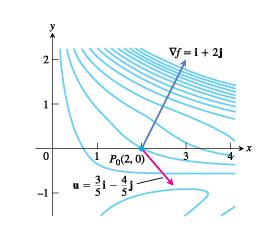
\includegraphics[width=0.45\linewidth]{graphics-14-28-thomas.jpg}
	\caption{A taxa com que $f$ varia na direção de $u$ é \(\nabla f\cdot u=-1$}
	\label{fig:14-28-thomas}
\end{figure}


%
\subsection{Propriedades da Derivada Direcional}
%

O cálculo do produto escalar na formula
\begin{equation*}
	D_{u}f = \nabla f\cdot u = |\nabla f||u|\cos \theta =|\nabla f| \cos \theta
\end{equation*}
onde \(\theta\) é o ângulo entre os vetores \(u\) e \(\nabla f\) revela-nos as propriedades a seguir.

\begin{figure}[!h]
	\centering
	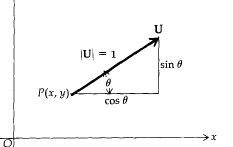
\includegraphics[width=0.3\linewidth]{calculus-directions-leithold.png}
	\caption{\(U\) é o vetor unitário \(\cos \theta \, i + \sen \theta\, j\) }\label{fig:17-7-1}
\end{figure}

\begin{figure}[!h]
	\centering
	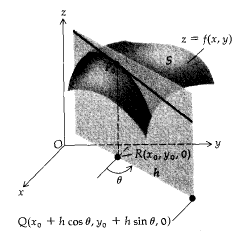
\includegraphics[width=0.3\linewidth]{calculus-directions-leithold01.png}
	\caption{Definição de derivada direcional com vetor unitário \(u=\cos\theta\,i +\sen \theta\, j\)}
	\label{fig:17-7-2}
\end{figure}

\begin{itemize}
	\item A função \(f\) aumenta mais rapidamente quando \(\cos \theta = 1\) ou quando \(u\) é a direção de \(\nabla f\).
	Isto é, a cada ponto \(P\) no seu domínio, \(\nabla\, f\) cresce mais rapidamente na direção  e no sentido do vetor gradiente \(\nabla f \) em \(P\). A derivada nessa direção é
	\begin{equation*}
		D_{u}f=|\nabla\, f|\cos 0 = |\nabla\, f|.
	\end{equation*}
	
	\item De maneira similar, \(f\) decresce mais rapidamente na direção e no sentido de \(-\nabla f \). A derivada nessa direção é
	\begin{equation*}
		D_{u}f=|\nabla f|\cos \pi = -|\nabla f|.
	\end{equation*}
	
	\item Qualquer direção \(u\) ortogonal ao gradiente \(\nabla\, f \neq 0\) é uma direção de variação zero em \(f\) porque \(\theta\) é então igual a \( \pi/2\) e
	\begin{equation*}
		D_{u}f=|\nabla\, f|\cos\left(\frac{\pi}{2} \right) = |\nabla\, f|\cdot 0= 0.
	\end{equation*}
\end{itemize}

Como veremos mais à frente, essas propriedades são verdadeiras tanto em três dimensões como em duas.
\begin{exc}[Direções de Variação Máxima, Mínima e Zero]
	Encontre as direções nas quais
	\begin{equation*}
		f(x,\; y) = \frac{x^{2}}{2} + \frac{y^{2}}{2}.
	\end{equation*}
	\begin{tasks}[label=(\alph*),item-indent=3em,label-width=4ex,ref=(\alph*)](2)
		\task Cresce mais rapidamente no ponto \((1,\; 1)\);
		\task Decresce mais rapidamente em \((1,\; 1)\);
		\task! Quais são as direções de variação zero de \(f\) em \((1,\; 1)\)?
	\end{tasks}
\end{exc}

\textbf{Solução.}

(a) A função aumenta mais rapidamente na direção e no sentido de \(\nabla f\) em \( (1,\; 1)\). O gradiente nesse ponto é
\begin{equation*}
	(\nabla f)_{(1,\; 1)}=(x\, i + y\, j)\Big\vert_{(1,\; 1)}=i+j.
\end{equation*}

Sua direção ou versor é,
\begin{equation*}
	u=\dfrac{(\nabla f)_{(1,\; 1)}}{|(\nabla f)_{(1,\; 1)}|} =\dfrac{i+j}{|i+j|}=\dfrac{i+j}{\sqrt{(1)^{2}+(1)^{2}}}=\frac{1}{\sqrt{2}}\, i + \frac{1}{\sqrt{2}}\, j
\end{equation*}

(b) A função decresce mais rapidamente na direção e no sentido de \(-\nabla f\) em \((1,\; 1)\), e sua direção ou versor é,
\begin{equation*}
	-u =-\dfrac{(\nabla f)_{(1,\; 1)}}{|(\nabla f)_{(1,\; 1)}|} =-\frac{1}{\sqrt{2}}\, i - \frac{1}{\sqrt{2}}\, j
\end{equation*}

(c) As direções de variação zero em \((1,\; 1)\) são as direções ortogonais a \(\nabla f\),
\begin{equation*}
	n=-\frac{1}{\sqrt{2}}\, i + \frac{1}{\sqrt{2}}\, j \quad \text{ e }\quad -n=\frac{1}{\sqrt{2}}\, i - \frac{1}{\sqrt{2}}\, j
\end{equation*}
Veja a Figura~\ref{fig:14-29-thomas}.

\begin{figure}[!h]
	\centering
	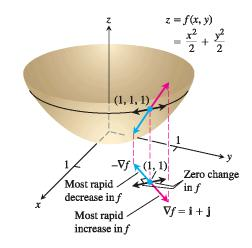
\includegraphics[width=0.4\linewidth]{graphics-14-29-thomas.jpg}
	\caption{A direção em que $f(x,\, y)$ aumenta mais rapidamente em \((1,\; 1)\) é
		a direção de \((\nabla f)_{(1,\, 1)}=i+j\). Corresponde à direção e ao sentido de subida mais íngreme na superfície em \((1,\, 1,\, 1)\)}
	\label{fig:14-29-thomas}
\end{figure}



%
\subsection*{Gradientes e Reta Tangente a Curvas de Nível}
%

Se uma função diferenciável \(f(x,\; y)\) tiver um valor constante \(C\) ao longo de uma curva lisa
\(\alpha(t) = g(t)\,i + h(t)\, j)\) (fazendo da curva uma curva de nível de \(f\)), então \(f(g(t),\; h(t))=C\).

Derivar ambos os lados dessa equação em relação a \(t\), usando a regra da cadeia leva às equações
\begin{equation*}
	\frac{d}{dt}f(g(t),\; h(t))  =\frac{d}{dt}\, C,
\end{equation*}
e pela regra da cadeia,
\begin{equation*}
	\frac{\partial\, f}{\partial x}\frac{dg}{dt}\, i + \frac{\partial\, f}{\partial y}\frac{dh}{dt}\, j  = 0.
\end{equation*}

Portanto,
\begin{equation}\label{eq:5-thom}
	\left(\frac{\partial f}{\partial x}\, i+\frac{\partial f}{\partial y}\, j \right)\cdot \left(\frac{dg}{dt}\, i + \frac{dh}{dt}\, j \right) = 0.
\end{equation}

A equação \eqref{eq:5-thom} diz que \(\nabla\, f\) é normal ao vetor tangente \(\alpha'(t)\), portanto é normal à curva.


Em todo ponto \((x_{0},\; y_{0})\) no domínio de uma função diferenciável \(f(x,\; y)\) o gradiente d e \(f\) normal à curva de nível que passa por \((x_{0},\; y_{0})\).

A equação \eqref{eq:5-thom} confirma nossa observação dc que os córregos correm perpendicularmente às curvas de nível em mapas topográficos.

Como o córrego deve alcançar seu destino da maneira mais rápida, deve correr na direção oposta á dos gradientes, devido a Propriedade 2 da derivada direcional. A equação \eqref{eq:5-thom} nos diz que essas direções são perpendiculares às curvas de nível.

Essa observação também nos permite encontrar equações para retas tangentes às curvas de nível. Elas são as retas normais aos gradientes. A reta que passa por um ponto \(P_{0}(x_{0},\;y_{0})\) normal a um vetor \(N = A\,i +B\,j\) tem a equação
\begin{equation*}
	A(x-x_{0})+B(y-y_{0})=0
\end{equation*}

Se \(N\) é o gradiente
\begin{equation*}
	(\nabla f)_{P_{0}}= \partial_{x}f(P_{0})\, i +\partial_{y}f(P_{0})\, j
\end{equation*}
a equação torna-se
\begin{equation}\label{eq:6-thom}
	\partial_{x}f(x_{0},\; y_{0})(x-x_{0})+\partial_{y}f(x_{0},\; y_{0})(y-y_{0})=0
\end{equation}

\begin{exc}[Reta Tangente a uma Elipse]
	Encontre uma equação para a tangente à elipse
	\begin{equation*}
		\frac{x^{2}}{4}+y^{2} =2
	\end{equation*}
	no ponto \((-2, \; 1)\).
\end{exc}

\solo
A elipse é uma curva de nível da função
\begin{equation*}
	f(x,\; y) = \frac{x^{2}}{4}+y^{2}
\end{equation*}

O gradiente de \(f\) em \((-2,\;  1)\)  é,
\begin{equation*}
	\nabla f\Big\vert_{(-2,\; 1)}=\left(\frac{x}{2}\, i + 2y\, j \right)\Bigg\vert_{(-2,\; 1)}= -i+2\, j
\end{equation*}

A tangente é a reta
\begin{equation*}
	(-1)(x+2)+(2)(y-1)=0
\end{equation*}

Assim
\begin{equation*}
	x-2y = -4
\end{equation*}

Se soubermos os gradientes de duas funções \(f\) e \(g\), automaticamente saberemos os gradientes de sua soma e diferença, de seu produto e quociente e da multiplicação por uma constante.

O estudante deverá justificar essas propriedades nas listas de Exercícios Propostos. Observe que elas tem a mesma forma que as propriedades correspondentes para derivadas de funções de uma variável

%
\subsection{Propriedades Algébricas do Vetor Gradiente}
%
Multiplicação por constante,
\begin{equation*}
	\nabla ( k\, f ) = k\, \nabla f \quad \text{para qualquer número}\quad  k.
\end{equation*}

Regra da Adição
\begin{equation*}
	\nabla( f+g) = \nabla f + \nabla g
\end{equation*}

Regra do produto
\begin{equation*}
	\nabla (fg) = f\, \nabla g + g\nabla\, f
\end{equation*}

Regra do Quociente
\begin{equation*}
	\nabla \left(\frac{f}{g} \right) = \frac{g\nabla f - f \nabla g}{g^{2}}
\end{equation*}

\bigskip
\begin{exc}
	Verificar as propriedades do gradiente utilizando as seguintes funções escalares,
	\begin{equation*}
		f(x,\, y)=x-y \quad \text{e} \quad g(x,\; y)=3y
	\end{equation*}
\end{exc}

\solo
Calculamos o gradiente de cada função rela de duas variáveis,
\begin{equation*}
	\nabla f = i-j\quad \text{ e } \quad \nabla g =3\,j.
\end{equation*}

Para uma constante qualquer \( k =2\),
\begin{equation*}
	\nabla(2f) = \nabla (2x-2y)=i+ 2\,j=2\,\nabla f
\end{equation*}

O gradiente da soma,
\begin{equation*}
	\nabla(f+g)= \nabla(x+2y) = i + 2\, j=\nabla f + \nabla g
\end{equation*}

O gradiente da soma,
\begin{equation*}
	\nabla(f-g)= \nabla(x-4y) = i -4\, j=\nabla f - \nabla g
\end{equation*}

O gradiente do produto,
\begin{align*}
	\nabla(f\, g) &= \nabla (3xy-3y^{2}) = 3y\, i +(3x-6y)\, j \\[2ex]
	&= 3y(i-j)+3y\,j+(3x-6y)\,j\\[2ex]
	&= 3y(i-j)+(3x-3y)\,j\\[2ex]
	&= 3y(i-j)+(x-y)3\,j = g\nabla f+ f\, \nabla g
\end{align*}

O gradiente do quociente
\begin{align*}
	\nabla\left(\frac{f}{g}\right) & = \nabla \left(\frac{x-y}{3y} \right)= \nabla \left(\frac{x}{3y}-\frac{1}{3}\right) \\
	& = \frac{1}{3y}\, i -\frac{x}{3y^{2}}\,j\\
	&=\dfrac{3y\,i-3x\,j}{9y^{2}}=\frac{3y(i-j)-(3x-3y)\, j}{9y^{2}}\\
	&=\frac{3y(i-j)-(x-y)3j}{9y^{2}}=\frac{g\nabla f-f\nabla g}{g^{2}}.
\end{align*}

%
\subsection{Funções Reais de Três Variáveis}
%
Para uma função diferenciável \(f(x,\; y,\; z)\) e um vetor unitário \(u = u_{1}\,i +u_{2}\,j+u_{1}\,k\) no espaço, temos
\begin{equation*}
	\nabla f = \frac{\partial f}{\partial x}\, e_{1}+\frac{\partial f}{\partial y}\, e_{2} +
	\frac{\partial f}{\partial z}\, e_{3}
\end{equation*}
e
\begin{equation*}
	D_{u}f= \nabla f \cdot u =\frac{\partial f}{\partial x}u_{1}+\frac{\partial f}{\partial x}u_{2}
	+\frac{\partial f}{\partial z}u_{3}
\end{equation*}

A derivada direcional pode ser escrita novamente na forma
\begin{equation*}
	D_{u}f= \nabla f \cdot u =|\nabla f||u| \cos \theta= |\nabla f|\cos \theta
\end{equation*}
assim as propriedades relacionadas anteriormente para funções de duas variáveis continuam valendo. Em qualquer ponto
dado, \(f\) aumenta mais rapidamente na direção de \(\nabla f\) e decresce mais rapidamente na direção de \(-\nabla
f\). Em qualquer direção ortogonal a \(\nabla f\) a derivada é zero,

\begin{exc}[Direções de variação máxima, mínima e zero]
	Resolva em detalhes as seguintes questões
	\begin{enumerate}
		\item[\rm{(a)}] Encontre a derivada de \(f(x,\; y,\; z) = x^{3}-xy^{2}-z\) em \(P_{0}(1,\; 1,\; 0)\) na direção de \(v = 2i
		-3j + 6\, k\).
		\item[\rm{(b)}] Em que direções \(f\) varia mais rapidamente em \(P_{0}\) e quais são as taxas de variação nessas direções?
	\end{enumerate}
\end{exc}

\solo
A direção de \(v\) é obtida dividindo-se \(v\) pelo seu comprimento,
\begin{equation*}
	|v|=\sqrt{(2)^{2}+(-3)^{2}+(6)^{2}}=\sqrt{49}=7
\end{equation*}
logo,
\begin{equation*}
	u=\frac{v}{|v|}=\frac{2}{7}\, i -\frac{3}{7}\, j+\frac{6}{7}\,k
\end{equation*}

As derivadas parciais de \(f\) em \(P_{0}\), são
\begin{equation*}
	\partial_{x}f=(3x^{2}-y^{2})\Big\vert_{(1,\;1, \; 0)}=2, \quad \partial_{y}f=-2xy\Big\vert_{(1,\;1, \; 0)}=-2, \quad \partial_{z}f=-1\Big\vert_{(1,\;1, \; 0)}=-1
\end{equation*}

O gradiente de \(f\) em \(P_{0}\) é
\begin{equation*}
	\nabla f\Big\vert_{(1,\; 1, \; 0)}=2\,i-2\,j-k.
\end{equation*}

A derivada direcional de \(f\) em \(P_{0}\) na direção de \(v\) é, portanto,
\begin{align*}
	(D_{u}f)_{(1,\;1,\; 0)} & = \nabla f\Big\vert_{(1,\; 1, \; 0)}\cdot u =(2i-2j-k)\cdot \left(\frac{2}{7}i-\frac{3}{7}\,j+\frac{6}{7}\, k \right) \\[2ex]
	&=\frac{4}{7}+\frac{6}{7}-\frac{6}{7}=\frac{4}{7}.
\end{align*}

(b) A função cresce mais rapidamente na direção de \( \nabla f = 2i - 2j-k\) e decresce mais rapidamente na direção
do vetor \(-\nabla f\). As taxas de variação nas direções são, respectivamente,
\begin{equation*}
	|\nabla f|=\sqrt{(2)^{2}+(-2)^{2}+(-1)^{2}}=\sqrt{9}=3 \quad \text{e} \quad -|\nabla f| =-3.
\end{equation*}

%
\section{Campos Vetoriais}
%

Um \textsf{campo vetorial} em \(\mathbb{R}^{n}\) é uma função \(\mathbf{F} \colon  A \subset \mathbb{R}^{n} \to  \mathbb{R}^{n}\) que atribui a cada
ponto \(\mathbf{x}\) em seu domínio \(A\) um vetor \(\mathbf{F}(\mathbf{x})\).  Se \(n = 2\), a função \(F\) é chamada de \textsc{campo vetorial no
	plano} e se \(n = 3\), a função \(\mathbf{F}\) é um \textsc{campo vetorial no espaço}.

O campo \(\mathbf{F}\) figura como anexado uma seta em cada ponto (Veja a Figura~\ref{fig:4-3-1}).
\begin{figure}[h]
	\centering
	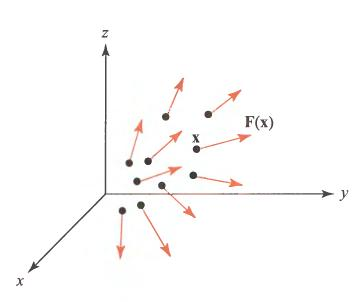
\includegraphics[width=3.0in]{figura-calculus-marsden431-col.jpg}
	\caption{Um campo vetorial \(\mathbf{F}\) atribui um vetor \(\mathbf{F}(\mathbf{x})\) a cada ponto \(\mathbf{x}\) de seu domínio }\label{fig:4-3-1}
\end{figure}

Em contraste, uma função \(f \colon  A \subset  \mathbb{R}^{n} \to \mathbb{R}\) que atribui um número a cada ponto de seu domínio é um \textsc{campo
	escalar}.

Um campo vetorial \(\mathbf{F}(x,\, y,\, z) \) em \(\mathbb{R}^{3} \)  tem \textsf{três campos escalares} componentes \(F_{1}\),  \(F_{2}\) e \(F_{3}\) de modo
que
\begin{equation*}
	\mathbf{F}(x,\, y,\, z) =\left(F_{1} (x, \, y,\,  z),\; F_{2} (x, \, y,\,  z),\;  F_{3} (x,\,  y,\,  z)\right).
\end{equation*}

Se cada uma das componentes \(F_{1}\), \(F_{2}\) e \(F_{3}\) é uma função de classe \(C^{k}\), dizemos que o campo vetorial \(\mathbf{F}\) é da classe \(C^{k}\), os campos vetoriais serão assumidos no que segue como sendo pelo menos da classe \(C^{1}\), a menos que indicado de outra forma.

Em muitas aplicações, \(\mathbf{F}(\mathbf{x})\) representa uma grandeza vetorial física (força, velocidade, etc.) associada à posição \(\mathbf{x}\).

Visualizamos campos vetoriais traçando a seta que representa $\mathbf{F}(x,\; y)$ no ponto $(x,\; y)$ ou $\mathbf{F}(x,\; y,\; z)$ em cada ponto
$(x,\; y,\; z)$.

Obviamente, não podemos fazer isso para todos os pontos, então fazemos isso para alguns pontos representativos. Também podemos usar software
matemático para plotar um campo vetorial. O comando em cada software para plotar um campo vetorial depende se é um campo vetorial em $\mathbb{R}^{2}$
ou $\mathbb{R}^{3}$.

%
\section{Operações de Divergência e Rotacional}
%

Para cada uma das operações de divergência e rotacional, faremos uso do operador ``del'', definido por
\begin{equation*}
	\nabla = i\, \partial_{x}+j\, \partial_{y}+k\, \partial_{z}
\end{equation*}

Para funções de uma variável, a obtenção de uma derivada pode ser considerada uma operação ou processo; isto é, dada uma função \(y = f (x)\), sua derivada é o resultado da operação em \(y\) pelo operador derivação \(D=d/dx\). Da mesma forma, podemos escrever o gradiente de \(f\) como
\begin{equation*}
	\nabla f =\left(i\, \partial_{x}+j\, \partial_{y}\right)\, f = i\, \partial_{x} f+j\, \partial_{y} f,
\end{equation*}
para funções de duas variáveis, e
\begin{equation*}
	\nabla f =\left( i\, \partial_{x}+j\, \partial_{y}+k\, \partial_{z}\right)\, f= i\, \partial_{x} f+j\, \partial_{y}f+k\, \partial_{z} f
\end{equation*}
para três variáveis. Em termos operacionais, \textsf{o gradiente de} \(f\) é obtido tomando o operador \(\nabla\) e aplicando-o para o \textsf{campo
	escalar} \(f\).

%
\subsection*{Definição da Divergência}
%

Definimos a divergência de um campo vetorial \(\mathbf{F}\) tomando o produto escalar do operador  \(\nabla\) com o campo vetorial \(\mathbf{F}\).

\begin{defi}[Divergência]
	Se \(\mathbf{F} =F_{1}\, i + F_{2}\, j + F_{3}\, k\) campo vetorial em $\mathbb{R}^{3}$, a divergência de \( \mathbf{F}\) é o campo escalar
	\begin{equation*}
		\mathrm{div}\, \mathbf{F}= \nabla\cdot \mathbf{F} = \partial_{x}F_{1}+ \partial_{y}F_{2}+\partial_{z}F_{3}
	\end{equation*}
\end{defi}

Da mesma forma, se \(\mathbf{F} = (F_{1},\ldots, F_{n})\) é um campo vetorial em \(\mathbb{R}^{n}\), sua divergência é
\begin{equation*}
	\mathrm{div}\, \mathbf{F} = \nabla \cdot F= \sum_{i=1}^{n}\partial_{x_{i}}F_{i}=\partial_{x_{1}}F_{1}+ \partial_{x_{2}}F_{2}+\cdots+\partial_{x_{n}}F_{n}
\end{equation*}

\begin{exc}
	Calcular a divergência do seguinte campo vetorial
	\begin{equation*}
		\mathbf{F}(x,\, y,\, z) = x^{2}y\,i + z\, j + xyz\, k.
	\end{equation*}
	em $\mathbb{R}^{3}$.
\end{exc}

\solo
Ao aplicar a definição de divergência devemos calcular primeiro as derivadas parciais na direção se sentido dos versores ou vetores
unitários canônicos, isto é,
\begin{equation*}
	\partial_{x}F_{1}(x,\, y, \, z)= 2xy ;  \quad \partial_{y}F_{2}(x,\, y, \, z)=0 ; \quad \partial_{z}F_{3}(x,\, y, \, z)=xy
\end{equation*}

Logo obtemos,
\begin{equation*}
	\mathrm{div}\, \mathbf{F} = \nabla \cdot \mathbf{F} = \partial_{x}F_{1}+\partial_{y}F_{2}+\partial_{z}F_{3} =2xy+0+xy=3xy
\end{equation*}
que é o \textsf{campo escalar divergência}. \hfill $\lozenge$

\bigskip
A divergência tem uma importante interpretação física. Se imaginarmos \(\mathbf{F}\) para ser o campo de velocidade de um gás (ou um fluido), então
\(\mathrm{div}\; \mathbf{F}\) representa a \textit{taxa de expansão por unidade de volume sob o fluxo do gás} (ou fluido). Se \(\mathrm{div}\; \mathbf{F} < 0\), o gás
(ou fluido) está comprimindo. Para um campo vetorial \(\mathbf{F}(x,\; y) = F_{1}\,i + F_{2}\, j\) no plano, a divergência,
\begin{equation*}
	\nabla\cdot \mathbf{F} = \partial_{x}F_{1}+\partial_{y}F_{2}
\end{equation*}
mede a taxa de expansão da área.

Esta interpretação é explicada graficamente, como segue. Escolha uma pequena região \(W\) com um ponto \(\mathbf{x}_{0}\). Para cada ponto
\(\mathbf{x}\) em \(W\), defina \(\mathbf{x}(t)\) ser a linha de fluxo emanando de \(\mathbf{x}\). O conjunto de pontos \(\mathbf{x}(t)\) descreve
como o conjunto \(W\) flui após o tempo \(t\) (veja a Figura~\ref{fig:4-4-1}).

\begin{figure}[H]
	\centering
	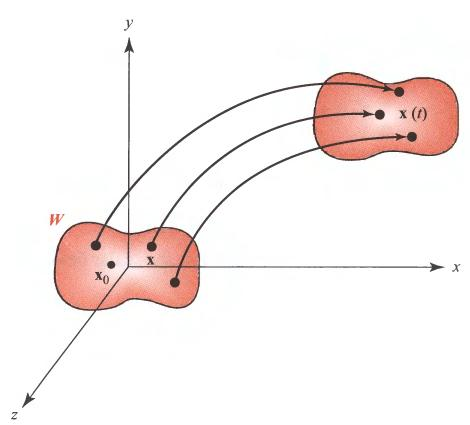
\includegraphics[width=0.4\linewidth]{figura-marsden441.jpg}
	\caption{ Uma região \(W\) fluindo ao longo das linhas de fluxo de um campo vetorial.}
	\label{fig:4-4-1}
\end{figure}

Denota-se para a região que resulta depois que o tempo \(t\) decorreu com \(W (t)\), e seja \(V(t)\)  seu volume (ou área em duas
dimensões). Então a \textit{taxa relativa de mudança de volume} é a divergência; mais precisamente,
\begin{equation*}
	\dfrac{1}{V(0)}\dfrac{d}{dt}V(t)\Bigg{\vert}_{t=0}\approx \mathrm{div\,}\mathbf{F}(0)
\end{equation*}
com a aproximação sendo mais exata quando \(W\) encolhe cada vez mais para \(\mathbf{x}_{0}\).

\begin{exc}
	Considere o campo vetorial num avião dado por \(\mathbf{V}(x,\; y) = x\, i\). Relacionar o sinal da divergência de \(\mathbf{V}\) com a taxa de mudança de
	áreas sob o fluxo.
\end{exc}

\solo Pensamos no campo vetorial \(\mathbf{V}\)  como o campo de velocidade de um fluido no plano. O campo vetorial \(\mathbf{V}\) aponta para a
direita quando \(x>0\) e à esquerda se \(x<0\), como vemos na Figura~\ref{fig:4-4-2}.

\begin{figure}[H]
	\centering
	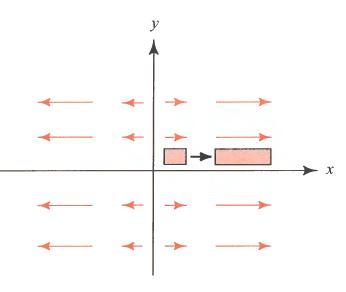
\includegraphics[width=0.5\linewidth]{figura-marsden442}
	\caption{O fluido está se expandindo.}
	\label{fig:4-4-2}
\end{figure}

O comprimento de \(\mathbf{V}\) fica mais curto em direção à origem. Como o fluido se move, ele se expande (a área do retângulo sombreado
aumenta), então esperamos \(\mathrm{div}\; \mathbf{V} > 0\). De fato, efetuando-se o calculo do campo escala divergência, valida-se a nossa conjectura,
isto é,
\begin{equation*}
	\mathrm{div}\; \mathbf{V} =\nabla\cdot \mathbf{V} = \partial_{x}V_{1}(x,\; y)+\partial_{y}V_{2}(x,\; y)=1+0=1 > 0
\end{equation*}

\begin{exc}
	As linhas de fluxo do campo vetorial \(\mathbf{F} = x\, i + y\, j\) são linhas retas direcionadas para longe da origem, relacionar o sinal do
	campo escalar divergência  com a taxa de expansão se as linhas de fluxo fossem de um fluído.
\end{exc}

\solo
Como linhas de fluxo são de um fluido, observamos que o fluido está se expandindo, pois se move afastando-se da origem, de modo que
\(\mathrm{div}\; \mathbf{F}\) deve ser positivo. Na verdade, calculando o divergente usando a definição obtemos,
\begin{equation*}
	\mathrm{div}\; \mathbf{F} =\nabla \cdot \mathbf{F}= \partial_{x}F_{1}(x,\; y)+\partial_{y}F_{2}(x,\; y)=1+1=2>0,
\end{equation*}
o que confirma a nossa afirmação. Veja a Figura~\ref{fig:4-4-3}.

\begin{figure}[H]
	\centering
	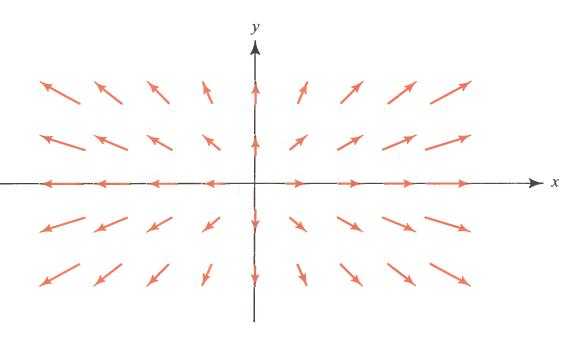
\includegraphics[width=0.5\linewidth]{figura-marsden443}
	\caption{O campo vetorial \(\mathbf{F}(x,\; y) = x\, i + y\, j\)}
	\label{fig:4-4-3}
\end{figure}

%
\section{O Rotacional de um Campo Vetorial}
%
Para calcular o rotacional, a segunda operação básica realizada em campos vetoriais, aplicamos o produto cruz do operador \(\nabla\) com o campo vetorial \(\mathbf{F}\).

\begin{defi}[Rotacional]
	Se \(\mathbf{F} = F_{1}\, i + F_{2}\, j + F_{3}\, k\) é um campo vetorial em $\mathbb{R}^{3}$,  o rotacional de \(\mathbf{F}\) é o campo vetorial em $\mathbb{R}^{3}$ dado por,
	\begin{align*}
		\nabla\times F &= \left(\partial_{y}F_{3}-\partial_{z}F_{2}\right)\,i +\left(\partial_{z}F_{1}-\partial_{x}F_{3}\right)\, j
		+\left(\partial_{x}F_{2}-\partial_{y}F_{1} \right)\, k \\[3ex]
		&=\left|\begin{array}[c]{ccc}
			i& j & k\\
			\partial_{x} & \partial_{y} & \partial_{z}\\
			F_{1} & F_{2} & F_{3}		
		\end{array}
		\right|.
	\end{align*}
\end{defi}

Se escrevermos o campo vetorial por \(\mathbf{F} = P\,i + Q\,j + R\,k\) em $\mathbb{R}^{3}$, que é notação alternativa, a mesma fórmula para o rotacional será,
\begin{align*}
	\nabla\times F &= \left(\partial_{y}R-\partial_{z}Q\right)\,i +\left(\partial_{z}P-\partial_{x}R\right)\, j
	+\left(\partial_{x}Q-\partial_{y}P \right)\, k \\[3ex]
	&=\left|\begin{array}[c]{ccc}
		i& j & k\\
		\partial_{x} & \partial_{y} & \partial_{z}\\
		P & Q & R		
	\end{array}
	\right|.	
\end{align*}

A seguir resolvemos alguns exercícios para fixar e reforçar algumas ideias e conceitos.
\begin{exc}
	Considere o campo vetorial em $\mathbb{R}^{3}$, \(\mathbf{F}(x,\; y,\; z) = x\, i + xy\, j + k\). Encontre o rotacional \(\nabla \times \mathbf{F}\).
\end{exc}

\solo
Usamos a fórmula do rotacional anterior,
\begin{equation*}
	\nabla \times \mathbf{F} =
	\left|\begin{array}[c]{ccc}
		i & j & k\\
		\partial_{x} & \partial_{y} & \partial_{z}\\
		x & xy & 1		
	\end{array}
	\right|	= (0-0)\, i - (0-0)\, j + (y-0)\, k= y\, k.
\end{equation*}

Assim,
\begin{equation*}
	\nabla \times \mathbf{F} = y\, k.
\end{equation*}
é o rotacional procurado. \hfill $\lozenge$


\begin{exc}
	Encontre o rotacional do campo vetorial  \(\mathbf{F}=xy\, i -\sen z\, j + k\) em $\mathbb{R}^{3}$.
\end{exc}

\solo
Aplicando a definição de rotacional ao campo vetorial,
\begin{equation*}
	\nabla \times \mathbf{F} =
	\left|\begin{array}[c]{ccc}
		i & j & k\\
		\partial_{x} & \partial_{y} & \partial_{z}\\
		xy & -\sen z & 1		
	\end{array}
	\right|	= \left|\begin{array}{cc}
		\partial_{y} & \partial_{z}\\
		-\sen z & 1
	\end{array} \right|\, i - \left|\begin{array}{cc}
		\partial_{x} & \partial_{z}\\
		xy & 1
	\end{array} \right|\, j + \left|\begin{array}{cc}
		\partial_{x} & \partial_{y}\\
		xy & -\sen z
	\end{array} \right|\, k
\end{equation*}

Portanto,
\begin{equation*}
	\nabla\times \mathbf{F} = \cos z\, i -x\, k,
\end{equation*}
é a resposta do rotacional procurado. \hfill $\lozenge$

Ao contrário da divergência, que pode ser definida em \(\mathbb{R}^{n}\) para qualquer \(n\), definimos o rotacional apenas no espaço
tridimensional (ou para campos vetoriais planares, em relação ao terceiro componente como zero).

O significado físico do rotacional será discutido no Capítulo posterior, quando estudarmos o teorema de Stokes. No entanto, podemos agora considerar
uma situação específica, em que o \textsf{rotacional} está associada a \textsf{rotações}.

\bigskip
A seguinte identidade é uma relação básica entre o gradiente e o rotacional, que deve ser comparada com o fato de que para qualquer vetor $\mathbf{v}$, temos que seu produto cruz resulta em  \(\mathbf{v} \times \mathbf{v} = 0\).

%
\subsection*{Rotacional de um Gradiente}
%
Para quaisquer campo escalar $f$ de classe $C^{2}$
\begin{equation*}
	\mathrm{rot}\; \nabla f = \nabla \times (\nabla f)= \mathbf{0}.
\end{equation*}

Ou seja, o \textsf{rotacional} de qualquer campo gradiente é o vetor zero.

\prova
Pela definição $\nabla f=(\partial_{x}f, \; \partial_{y}f, \; \partial_{z}f )$, assim outra vez pela definição de rotacional,
\begin{align*}
	\mathrm{rot}\; \nabla f =\nabla \times \nabla f &=
	\begin{vmatrix}
		i & j & k \\
		\partial_{x} & \partial_{y} & \partial_{z} \\
		\partial_{x}f & \partial_{y}f & \partial_{z}f
	\end{vmatrix}\\[2ex]
	&=\left(\partial_{yz}^{2}f-\partial_{zy}^{2}f \right)\,i+\left(\partial_{zx}^{2}f-\partial_{xz}^{2}f \right)\,j+\left(\partial_{xy}^{2}f
	-\partial_{yx}^{2}f \right)\,k=\mathbf{0}.
\end{align*}

Cada componente é zero devido à igualdade das derivadas parciais mistas. \hfill $\square$

\begin{exc}
	Seja o campo vetorial $\mathbf{V}(x,\; y, \; z)=y\, i-x\, j$ em $\mathbb{R}^{3}$. Mostre que $\mathbf{V}$ não é um campo gradiente
\end{exc}

\solo
Se o campo vetorial $\mathbf{V}$ fosse um campo gradiente, então ele satisfaria $\nabla\times \mathbf{V} = \mathbf{0}$ pela afirmação mostrada anteriormente. Mas o rotacional de $\mathbf{V}$ é,
\begin{equation*}
	\mathrm{rot}\, \mathbf{V} = \nabla\times V=
	\begin{vmatrix}
		i & j & k \\
		\partial_{x} & \partial_{y} & \partial_{z} \\
		y & -x & 0
	\end{vmatrix}= -2\,k  \neq \mathbf{0}
\end{equation*}
que é  contraditório, logo $\mathbf{V}$ não e um campo gradiente. \hfill $\lozenge$

\bigskip
Existe uma operação em campos vetoriais no plano que está intimamente relacionada ao rotacional. Se $\mathbf{F} = P(x,\; y)\,i + Q(x,\; y)\,j$ é um campo
vetorial no plano, ele também pode ser considerado como um campo vetorial no espaço para o qual o componente $k$ é zero e os outros dois componentes são independentes de $z$. O rotacional de $F$ então se reduz a
\begin{equation*}
	\nabla \times \mathbf{F} = \Bigl(\partial_{x}\, Q(x,\; y) -\partial_{y}\, P(x,\; y)\Bigr)\, k
\end{equation*}
e sempre aponta na direção de $k$. A função
\begin{equation*}
	\partial_{x}\, Q(x,\; y) -\partial_{y}\, P(x,\; y)
\end{equation*}
de $x$ e $y$ é chamado de \textsf{rotacional escalar} de $\mathbf{F}$.

\begin{exc}
	Encontre o rotacional escalar do campo vetorial plano, dado por $\mathbf{V}(x,\; y) = -y^{2}\,i + x\, j$
\end{exc}

\solo
O rotacional é
\begin{equation*}
	\mathrm{rot}\; \mathbf{V} =\nabla \times \mathbf{V}=
	\begin{vmatrix}
		i & j & k \\
		\partial_{x} & \partial_{y} & \partial_{z} \\
		-y^{2} & x & 0
	\end{vmatrix}= (1+2y)\, k
\end{equation*}
então o \textsf{rotacional escalar}, que é o coeficiente do versor $k$, é dada pela relação $1+2y$. \hfill $\lozenge$

\bigskip
Uma relação básica entre as operações de divergência e rotacional é fornecida a seguir.
%
\subsection*{Divergência de um Rotacional}
%

Para qualquer campo vetorial $\mathbf{F}$ em $\mathbb{R}^{3}$ de classe $C^{2}$,
\begin{equation*}
	\mathrm{div}\;\mathrm{rot}\; \mathbf{F}=\nabla\cdot (\nabla\times \mathbf{F})=0.
\end{equation*}

Ou seja, a divergência de qualquer rotacional é zero.

Tal como acontece com a rotacional de um gradiente, a prova baseia-se na igualdade das derivadas parciais mistas. O estudante da disciplina deve
escrever os detalhes.

\bigskip
\begin{exc}
	Mostre que o campo vetorial $\mathbf{V}(x,\; y,\; z) = x\,i + y\,j + z\,k$  em $\mathbb{R}^{3}$ não pode ser o rotacional de algum campo vetorial $\mathbf{F}$, ou seja, não existe $\mathbf{F}$ tal que  $\mathbf{V} = \mathrm{rot}\; \mathbf{F}= \nabla\times \mathbf{F}$
\end{exc}

\solo
Se fosse assim, $\mathrm{div}\; \mathbf{V}$ seria zero pela propriedade mostrada anteriormente. Mas
\begin{equation*}
	\mathrm{div}\; \mathbf{V}= \nabla\cdot \mathbf{V}=\partial_{x}\, x + \partial_{y}\, y+ \partial_{z}\, z=1+1+1=3 \neq 0,
\end{equation*}
então $\mathbf{V}$ não pode ser $\mathrm{rot}\; \mathbf{F}$ para qualquer $\mathbf{F}$. \hfill $\lozenge$

%
\section{O Operador Laplaciano}
%

O operador de Laplace \(\nabla^{2}\), que opera em campos escalares \(f\), é definido para ser a divergência do gradiente,
\begin{equation*}
	\nabla^{2}f = \mathrm{div}\; \nabla f=\nabla\cdot \left( \nabla f\right) = \partial_{x}^{2}f+ \partial_{y}^{2}f+\partial_{z}^{2}f
\end{equation*}

Este operador desempenha um papel importante em muitas leis físicas.
\begin{exc}\label{exer:1-4}
	Mostre que \(\nabla^{2}f = 0\) para o campo escalar
	\begin{equation*}
		f(x,\; y, \; z)=\dfrac{1}{\sqrt{x^{2}+y^{2}+z^{2}}}=\dfrac{1}{|r|}\quad \text{ e } \quad (x,\; y,\; z) \neq (0,\; 0,\; 0)
	\end{equation*}
	onde \(r =x\, i + y\, j+ z\, k\)
\end{exc}

\solo
As primeiras derivadas parciais são,
\begin{equation*}
	\partial_{x}f=\dfrac{-x}{(x^{2}+y^{2}+z^{2})^{3/2}}, \quad \partial_{y}f=\dfrac{-y}{(x^{2}+y^{2}+z^{2})^{3/2}},
	\quad \partial_{z}f=\dfrac{-z}{(x^{2}+y^{2}+z^{2})^{3/2}}.
\end{equation*}

Computando as segundas derivadas, obtemos
\begin{align*}
	\partial^{2}_{x}f=\dfrac{3x^{2}}{(x^{2}+y^{2}+z^{2})^{5/2}}-\dfrac{1}{(x^{2}+y^{2}+z^{2})^{3/2}}\\[2ex]
	\partial^{2}_{x}f=\dfrac{3y^{2}}{(x^{2}+y^{2}+z^{2})^{5/2}}-\dfrac{1}{(x^{2}+y^{2}+z^{2})^{3/2}}\\[2ex]
	\partial^{2}_{x}f=\dfrac{3z^{2}}{(x^{2}+y^{2}+z^{2})^{5/2}}-\dfrac{1}{(x^{2}+y^{2}+z^{2})^{3/2}}
\end{align*}

Assim obtemos,
\begin{align*}
	\partial_{x}^{2}f+\partial_{y}^{2}f+\partial_{z}^{2}f &=
	\dfrac{3(x^{2}+y^{2}+z^{2})}{(x^{2}+y^{2}+z^{2})^{5/2}}-\dfrac{3}{(x^{2}+y^{2}+z^{2})^{3/2}}\\[2ex]
	&=\dfrac{3}{(x^{2}+y^{2}+z^{2})^{3/2}}-\dfrac{3}{(x^{2}+y^{2}+z^{2})^{3/2}}
\end{align*}


\begin{exc}\label{exer:1-5}
	Justifique a seguinte identidade,
	\begin{equation*}
		\mathrm{div}\left(f\, \mathbf{F} \right)= f\, \mathrm{div}\, \mathbf{F}+ \mathbf{F}\cdot \nabla f
	\end{equation*}
\end{exc}

\solo
O campo vetorial \(f\,\mathbf{F}\) tem componentes \(f\,F_{i}\), para \(i = 1,\; 2,\; 3\) e assim
\begin{equation*}
	\mathrm{div}\,\left(f\, \mathbf{F}\right) = \partial_{x}\left(f\, F_{1} \right)+\partial_{y}\left(f\, F_{2}\right)+\partial_{z}\left(f\,F_{3}\right).
\end{equation*}

Contudo,
\begin{equation*}
	\partial_{x}\left(f\, \mathbf{F}\right) = f\, \partial_{x}F_{1}+F_{1}\partial_{x}f
\end{equation*}
pela regra do produto, com expressões semelhantes para os demais termos. Portanto,
\begin{align*}
	\mathrm{div}\,\left(f\, \mathbf{F}\right) = f\Bigl(\partial_{x}F_{1}+\partial_{y}F_{2}+\partial_{z}F_{3}\Bigr) +
	F_{1}\partial_{x}f+F_{2}\partial_{x}f+F_{3}\partial_{z}f
\end{align*}

Vamos usar essas identidades para refazer o Exercício~\ref{exer:1-4}.

\begin{exc}\label{exer:1-6}
	Mostre ou justifique a seguinte identidade,
	\begin{equation*}
		\nabla^{2}\left(\dfrac{1}{|r|}\right) =0,
	\end{equation*}	
	sendo a função de posição \(r=x\, i+y\, j + z\, k \neq 0\,i + 0\, j+ 0\, k=\mathbf{0}\) é não nula.
\end{exc}

\solo
Como no caso do potencial gravitacional,
\begin{equation*}
	\nabla\left(\dfrac{1}{|r|} \right) =\dfrac{-r}{|r|^{3}}
\end{equation*}
em geral, \(\nabla(|r|^{n})=n\, |r|^{n-2}\,r\), com $n \in \mathbb{Z}$.

Utilizando a identidade
\begin{equation*}
	\nabla\cdot \left(f\, \mathbf{F} \right) =f\, \nabla\cdot \mathbf{F} + \nabla f \cdot \mathbf{F}
\end{equation*}
e identificando $f=-1/|r|^{3}$  e $\mathbf{F}= r$, obtemos
\begin{align*}
	\nabla\cdot \left(-\dfrac{r}{|r|^{3}} \right) &=-\dfrac{1}{|r|^{3}}\nabla\cdot r + r\cdot \nabla\left(-\dfrac{1}{|r|^{3}}\right)\\[2ex]
	&=-\dfrac{3}{|r|^{3}} + r \cdot \left(\dfrac{3\,r}{|r|^{5}} \right)=-\dfrac{3}{|r|^{3}}+\dfrac{3}{|r|^{3}}= 0.
\end{align*}
e isso mostra a identidade requerida. \hfill $\lozenge$

%
\subsection*{Identidades Básicas de Análise Vetorial}
%
Agora temos essas operações básicas em mãos: gradiente, divergência, rotacional e o operador de Laplace. A tabela a seguir contém algumas
fórmulas gerais básicas que são úteis ao calcular com campos vetoriais.
\begin{table}[H]
	\centering
	\begin{tabular}{>{\centering}m{1cm}|l}
		\toprule[2pt]
		1	&  \(\nabla\, (f + g) = \nabla f + \nabla g \) \\
		\midrule
		2	&  \(\nabla (cf) = c \nabla f\),  para uma constante \(c\)   \\
		\midrule
		3	& \( \nabla (fg) = f\, \nabla g + g\, \nabla f \)  \\
		\midrule
		4	& \(\nabla(f/g) = (g \nabla f - f \nabla g)/g^{2} \), em pontos \(x\) onde  \(g(x)\neq  0\) \\
		\midrule
		5	& \(\mathrm{div} (F + G) = \mathrm{div}\; F + \mathrm{div}\; G\) \\
		\midrule
		6	& \( \mathrm{rot}\; (F + G) = \mathrm{rot}\; F + \mathrm{rot}\; G \) \\
		\midrule
		7	& \( \mathrm{div}\; (f\,F) = f\; \mathrm{div}\; F + F \cdot \nabla f \) \\
		\midrule
		8	& \(\mathrm{div} (F \times G) = G \cdot \mathrm{rot}\; F - F \cdot \mathrm{rot}\; G\)\\
		\midrule
		9	& \(\mathrm{div}\; \mathrm{rot}\; F = 0\) \\
		\midrule
		10	& \(\mathrm{rot}\; (f\,F) = f \;\mathrm{rot}\; F + \nabla f \times F\) \\
		\midrule
		11	&  \(\mathrm{rot}\; \nabla f = 0\) \\
		\midrule
		12	&  \(\nabla^{2} (f\,g) = f\, \nabla^{2} g + g \nabla^{2} f + 2(\nabla f \cdot \nabla g)\) \\
		\midrule
		13	&  \(\mathrm{div}\; (\nabla f \times \nabla g) = 0\)\\
		\midrule
		14	& \(\mathrm{div}\; (f\; \nabla g - g \nabla f) = f \nabla^{2} g - g\nabla^{2} f\) \\
		\bottomrule[2pt]
	\end{tabular}
\end{table}

%%%%
\chapter{Funções Reais de Várias Variáveis}\label{chap:02}
%%%%%
Uma função $f$ real de várias variáveis, $f\colon D\subset \mathbb{R}^n\to B\subset\mathbb{R}$ é uma correspondência de um conjunto $D$ de vetores de 
$\mathbb{R}^n$ (ou uma \(n\)-upla de números reais) para um conjunto $B$ de números reais, de maneira que para cada vetor $\mathbf{x}=(x^1,\; x^2,\; x^3,\ldots,x^{n-1},\; x^n)\in D$ 
existe um único elemento $f(\mathbf{x})\in B$. O conjunto \(D=D_{f}\) é chamado de \textit{domínio da função} e o conjunto \(B\) é chamado de \textit{contradomínio da função} ou imagem.


O conjunto de todos os valores possíveis de \(\mathbf{x}\) (no caso, o conjunto
\(D\)) é chamado de domínio da função. O conjunto de todos os valores possíveis para \(f(\mathbf{x})\) é chamado de imagem da função.

%-----------
\subsection{\textcolor[rgb]{0.98,0.00,0.00}{Notações e Nomenclatura}}
%
O valor real da função $f$ de denota por $z=f(\mathbf{x})$. As variáveis $\mathbf{x}=(x^1,\; x^2,\ldots,x^{n})$ são chamadas de variáveis 
\emph{independentes} da função. Finalmente a variável $z$ é chamada de variável \emph{dependente}.

Em particular se \(n=1\), \(\mathbf{x}=x\); se \(n=2\), \(\mathbf{x}=(x,\; y)\); se \(n=5\), \(\mathbf{x}=(x^{1},\; x^{2},\; x^{3},\; x^{4},\; x^{5})\), e assim por diante.

\begin{defi}\label{new01}
	O conjunto dado por,
	\begin{equation*}
		D_{f}=\Bigl\{ \mathbf{x}\in \mathbb{R}^n \; \colon \; z=f(\mathbf{x})\in \mathbb{R} \Bigr\},
	\end{equation*}
	é chamado domínio de definição ou domínio de existência da função $f$.
\end{defi}

\begin{exer}\label{exe:1-1} 
	Considere a função $f\colon \mathbb{R}^2\to \mathbb{R}$ definida pela lei de correspondência.
	\begin{equation*}
		f(x, \;y)=\sqrt{9-x^2-y^2}
	\end{equation*}
	Determine seu domínio e faça o gráfico	
\end{exer}

\solo
A cada ponto \(\mathbf{x}=(x, y)\) pertencente a \(D_{f}\subsetneq \mathbb{R}^{2}\) podemos fazer corresponder um número \(z \in \mathbb{R}\), dado por
\begin{equation*}
	z=f(x,\;y)=(9-x^{2}-y^{2})^{1/2}
\end{equation*}

Neste caso, estamos diante de uma função real de duas variáveis reais denotada por
\begin{align*}
	f \; \colon D_{f} &\longrightarrow \mathbb{R}\\
	(x,\; y) &\longmapsto z=f(x,\; y)
\end{align*}

Esta função pode representar, por exemplo, a temperatura em uma chapa circular de raio \(r=3\). 


Pela definição de raiz quadrada, temos que a seguinte desigualdade é válida,
\begin{equation*}
	9-x^2-y^2\geq 0\quad \text{ logo}\quad 9\geq x^2+y^2.
\end{equation*}

O conjunto \(D_{f} \subsetneq \mathbb{R}^{2}\), isto é, o conjunto de pontos \((x,\;y)\in \mathbb{R}^{2}\) tais que 
\(9-x^{2}-y^{2}  \geq 0\) ou \(x^{2}+y^{2} \leq  9\) é chamado o domínio dessa função, e é denotado por
\begin{equation*}
	D_{f}=\Bigl\{(x, \; y)\in \mathbb{R}^2\; \colon\; x^2+y^2\leq 9 \Bigr\}
\end{equation*}


A representação geométrica deste domínio esta dado pelo círculo fechado de raio três. Veja a Figura~\ref{fig:dom-01} 

A imagem dessa função é o conjunto dos números \(z \in \mathbb{R}\), tais que \(0 \leq  z \leq 3\), e é denotada por
\begin{equation*}
	\mathrm{Im}(f)=\Bigl\{ z \in \mathbb{R}\;\colon\; 0 \leq z \leq 3 \Bigr\}
	\quad \text{ou} \quad \mathrm{Im}(f)=[0,\; 3]
\end{equation*}
e assim esta concluído o exercício. \hfill \(\lozenge\)
%
\begin{figure}[H]
	\centering
	\begin{subfigure}[b]{0.45\textwidth}
		\centering
		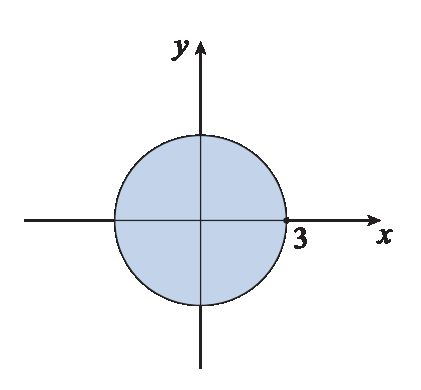
\includegraphics[width=0.7\textwidth]{circle-function01.jpg}
		\caption{Domínio da função \(f\)}
		\label{fig:dom-01-1}
	\end{subfigure}
	\hfill
	\begin{subfigure}[b]{0.45\textwidth}
		\centering
		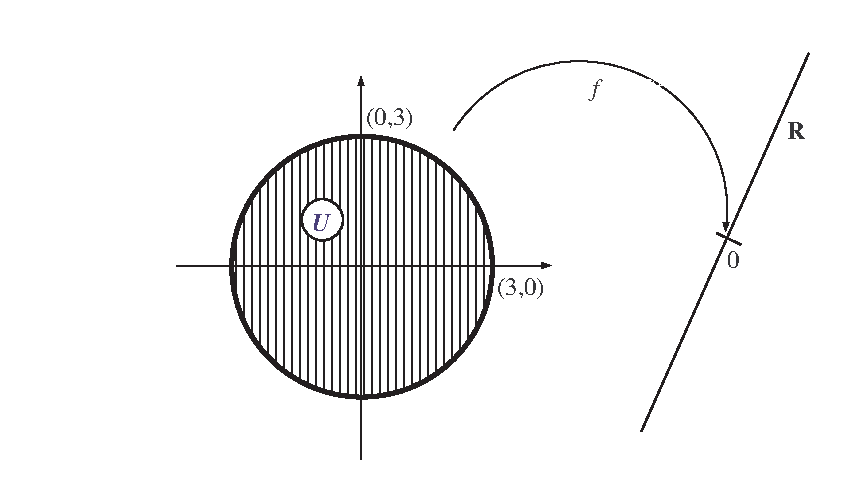
\includegraphics[width=\textwidth]{dominio01.eps}
		\caption{A correspondência $f$}
		\label{fig:dom-01-2}
	\end{subfigure}
	\caption{Domínio e correspondência da função \(f\)}
	\label{fig:dom-01}
\end{figure}
%

Salientamos que, para que tenhamos uma função, cada ponto \(\mathbf{x}\)
do conjunto \(D\) deve ser associado a apenas um número real \(z\).  De outra forma, se 
\(f(\mathbf{x}_{1}) = z_{1}\) e \(f(\mathbf{x}_{1}) = z_{2}\) , e \(f\) é uma função, então obrigatoriamente \(z_{1} = z_{2}\) .

Quando uma função \(f\) é dada através de alguma expressão termos \(\mathbf{x}\) de e nada é dito 
sobre seu domínio, entende-se que o domínio  é o maior conjunto de no qual a expressão dada faz
sentido como um número real.

\begin{exer}\label{exe:1-2-1}
	Encontre  o domínio da função real de duas variáveis definida por 
	\begin{equation*}
		f(x,\; y)= \ln(x-y)
	\end{equation*}
\end{exer}

\solo
A função real definida por \(f(x,\; y)= \ln(x-y)\)  é uma função de duas variáveis. Portanto, o seu domínio \(D_{f}\) é um subconjunto do \(\mathbb{R}^{2}\).

Pela definição da função logaritmo, temos que \(z=\ln(x-y)\) é um número real quando \(x-y>0\) ou
\(x>y\).

Assim, o domínio da função real \(f\) é 
\begin{equation*}
	D_{f} =\Bigl\{(x,\;y)\in \mathbb{R}^{2}\; \colon \; x>y \Bigr\}
\end{equation*}
e assim obtemos o conjunto desejado. \hfill \(\lozenge\)

A figura~\ref{fig:1-5} mostra a região do \(\mathbb{R}^{2}\) que representa graficamente esse domínio
\begin{figure}[H]
	\centering
	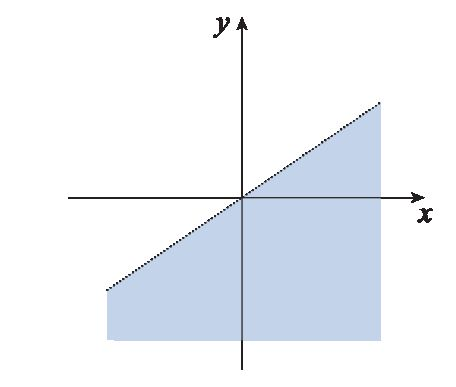
\includegraphics[width=0.5\textwidth]{logarihtmic-function01.jpg}
	\caption{Domínio da função \(\ln(x-y)\)}
	\label{fig:1-5}
\end{figure}

\begin{exer}\label{exe:1-3-1}
	Encontre o domínio da função real \(g\) de três variáveis definida por 
	\begin{equation*}
		g(x,\; y,\; z)= (25-x^{2}-y^{2}-z^{2})^{1/2}
	\end{equation*}
\end{exer}

\solo
A função real \(g\) possui  três variáveis independentes, logo seu domínio \(D_{g}\)é um subconjunto do \(\mathbb{R}^{3}\).

Pela definição da raiz quadrada podemos afirmar que \(z=g(\mathbf{x})\) é um numero real sempre 
\begin{equation*}
	25-x^{2}-y^{2}-z^{2} \geq 0  \quad \text{ou}\quad  x^{2}+y^{2}+z^{2} \leq 25
\end{equation*}

Assim, o domínio da função real \(g\) é dado por
\begin{equation*}
	D_{g} = \Bigl\{ \mathbf{x} \in \mathbb{R}^{3} \; \colon\; x^{2}+y^{2}+z^{2} \leq 25 \Bigr\}
\end{equation*}
e é representado pela região esférica do \(\mathbb{R}^{3}\) de raio \(r=5\), mostrada na figura~\ref{fig:1-6-1}
\begin{figure}[H]
	\centering
	\includegraphics[width=0.5\textwidth]{spheric-function01.jpg}
	\caption{Domínio da função \(z=g(\mathbf{x})\)}
	\label{fig:1-6-1}
\end{figure}
%
\begin{exer}\label{exe:1-2}
	Considere a função $g\colon \mathbb{R}^2\to \mathbb{R}$ definida por
	\begin{equation*}
		g(x,\;y)=\dfrac{1}{3}\sqrt{36-4x^{2}-9y^{2}}
	\end{equation*}
	Encontre seu domínio e imagem. Depois esboce seu gráfico.
\end{exer}

\solo Pela definição de raiz quadrada $36-4x^2-9y^2\geq 0$. Então o domínio da função $g$ esta definida pelo conjunto
\begin{equation*}
	D_{g}=\Bigl\{(x,\; y)\in \mathbb{R}^2\; \colon\; 36-4x^2-9y^2\geq 0\; \Bigr\}=\left\{(x,\; y)\in \mathbb{R}^2\; \colon\;  \frac{x^2}{3^2}+\frac{y^2}{2^2}\leq 1 \right\}.
\end{equation*}

A imagem ou o conjunto imagem é obtida pela manipulação algébrica da relação,
\begin{equation*}
	z=\dfrac{1}{3}\sqrt{36-4x^{2}-9y^{2}}\quad \Leftrightarrow \quad z=\sqrt{\dfrac{36-4x^{2}-9y^{2}}{9}}=\sqrt{4-(4/9)x^{2}-y^{2}}
\end{equation*}  
logo podemos determinar a variação da variável \(z\) da seguinte maneira,
\begin{equation*}
	z=\sqrt{4-(4/9)x^{2}-y^{2}} \geq 0 \quad \Leftrightarrow \quad 4-(4/9)x^{2}-y^{2} \geq 0
\end{equation*}
e observamos as possibilidades
\begin{equation*}
	z= 0 \quad \Leftrightarrow \quad  4-(4/9)x^{2}-y^{2}=0 \quad \Leftrightarrow\quad 4=(4/9)x^{2}+y^{2}
	\quad \Leftrightarrow \quad 1= \dfrac{x^{2}}{3^{2}}+\dfrac{y^{2}}{2^{2}}
\end{equation*}
ou seja atingimos o valor mínimo da superfície na fronteira da elipse, também
\begin{equation*}
	z > 0 \quad \Leftrightarrow \quad \dfrac{x^{2}}{3^{2}}+\dfrac{y^{2}}{2^{2}} <1
\end{equation*}
em pontos no interiores da elipse, nos pontos \((x,\; 0)\) dos eixos coordenados
\begin{equation*}
	z=\sqrt{4-(4/9)x^{2}}\quad \Leftrightarrow\quad (4/9)x^{2} +z^{2}=4 \quad 
	\Leftrightarrow\quad \left(\dfrac{x}{3}\right)^{2}+\left(\dfrac{z}{2}\right)^{2}=1
\end{equation*} 
temos uma elipse no eixos \(xz\) e nos pontos \((0,\; y)\) obtemos,
\begin{equation*}
	z=\sqrt{4-y^{2}}\quad \Leftrightarrow\quad y^{2}+z^{2}=4
\end{equation*}
que é uma circunferência no plano \(yz\) de raio \(2\).

Nos pontos da diagonal \((x,\; x)\) obtemos
\begin{equation*}
	z = \sqrt{4-(13/9)x^{2}} \quad \Leftrightarrow \quad \frac{13}{36}\,x^{2}+\dfrac{1}{4}\,z^{2}=1,
\end{equation*}
que é uma elipse no plano \(x=y\). 

Finalmente no ponto \((0,\; 0)\)
\begin{equation*}
	z=\sqrt{4-(4/9)x^{2}-y^{2}} \quad \Leftrightarrow\quad z= \sqrt{4} =2 
\end{equation*}
ou seja atingimos o valor máximo da superfície no ponto \((0,\; 0)\). 

A partir dessas informações podemos formular conjunto imagem
\begin{equation*}
	\textrm{Im}(g)=\Bigl\{z\in \mathbb{R} \; \colon \;  0\leq z \leq 2 \; \Bigr\}.
\end{equation*}

O gráfico é mostrada na Figura~\ref{dom_03} \hfill \(\lozenge\)

\begin{exer}
	Determine o domínio ``mais amplo'' das seguintes funções com leis de correspondência
	\begin{align*}
		\rm{(a)} & \quad  f(x,\; y)= \sqrt{x^{2}\,y\;}   \quad & \rm{(b)}& \quad f(x,\; y)= \ln\Bigl[(x-1)(y-1)\Bigr]
	\end{align*}
\end{exer}

\solo (a)  O valor da imagem \(z\) é um número real quando \(x^{2}y \geq 0\), isto é, pela lei de sinas no produto, \( y \geq 0\) e \( x \in \mathbb{R}\). Portanto obtemos
\begin{equation*}
	D_{f} = \left\{(x,\; y) \in \mathbb{R}^{2}\; \colon \; y \geq 0  \right\}
\end{equation*}

O semi-plano superior esta mostrado na seguinte Figura~\ref{fig:1-57} 
%
\begin{figure}[H]
	\centering
	\includegraphics[width=0.55\textwidth]{dominio-2d.jpg}
	\caption{Domínio da função de duas variáveis}
	\label{fig:1-57}
\end{figure}
%

(b)
O valor da imagem \(z\) é um número real  se \( (x-1)(y-1) > 0\). Assim sendo,
\begin{equation*}
	D_{f} = \Bigl\{(x,\; y) \in \mathbb{R}^{2}\; \colon\; (x-1)(y-1) > 0\; \Bigr\}
\end{equation*}

Pela lei de sinais no produto de fatores dados, obtemos a partir do conjunto  
\begin{equation*}
	\left\{(x,\; y)\in \mathbb{R}^{2}\colon x-1>0, \; y-1 > 0  \right\} \cup \left\{ (x,\; y)\in \mathbb{R}^{2}\colon x-1 < 0, \; y-1 < 0 \right\}
\end{equation*} 
a descrição do domínio \(D_{f}\) esta dada na Figura~\ref{fig:1-55} \hfill \(\lozenge\)
%
\begin{figure}[H]
	\centering
	\includegraphics[width=0.7\textwidth]{dominio-2d-02.jpg}
	\caption{}
	\label{fig:1-55}
\end{figure}
%

\begin{exer}
	Determine o domínio ``mais amplo'' das seguintes funções com leis de correspondência
	\begin{align*}
		\rm{(a)} & \quad  f(x,\; y)= \sqrt{y^{2}-4x^{2}}   \quad & \rm{(b)}& \quad f(x,\; y)= \dfrac{2}{xy-1}
	\end{align*}
\end{exer}

\solo (a)  A partir da definição da raiz temos \(y^{2}-4x^{2} \geq 0\) para que  \(z\) seja um numero real. Portanto
\begin{equation*}
	D_{f} = \Bigl\{(x,\; y) \in \mathbb{R}^{2}\; \colon\; y^{2}-4x^{2} \geq 0 \; \Bigr\}.
\end{equation*} 

Por outro lado a inequação,
\begin{equation*}
	y^{2}-4x^{2} \geq 0 \quad \Leftrightarrow \quad (y-2x)(y+2x) \geq 0
\end{equation*}
que também equivalente à
\begin{equation}\label{eq:1-3-1}
	y-2x \geq 0 \quad \textrm{e} \quad y+2x \geq 0
\end{equation}
ou 
\begin{equation}\label{eq:1-3-2}
	y-2x \leq 0 \quad \textrm{e} \quad y+2x \leq 0
\end{equation}

O gráfico cartesiano da relação \eqref{eq:1-3-1} juntamente com a segunda relação \eqref{eq:1-3-2} é nado no seguinte Figura~\ref{fig:1-6}
%
\begin{figure}[H]
	\centering
	\includegraphics[width=0.6\textwidth]{dominio-2d-03.jpg}
	\caption{}
	\label{fig:1-6}
\end{figure}
%

Assim o domínio \(D_{f}\) é o conjunto dos pontos \(\mathbb{R}^{2}\) da seguinte forma
\begin{equation*}
	D_{f} = \Bigl\{(x,\; y) \in \mathbb{R}^{2}\; \colon \; \left(y \geq 2x \quad \textrm{e} \quad y \geq -2x\right)
	\quad \textrm{ou}\quad \left(y \leq 2x \quad \textrm{e} \quad y \leq -2x\right) \Bigr\}
\end{equation*}

(b) A partir do denominador \( xy-1 \neq 0\) temos que \(f(x,\; y)\) é valor real. Assim, podemos escrever o domínio,
\begin{equation*}
	D_{f}= \Bigl\{(x,\; y)\in \mathbb{R}^{2}\; \colon\; xy \neq 1\; \Bigr\}
\end{equation*}
é um conjunto de pontos em \(\mathbb{R}^{2}\), excepto os pares que formam a hipérbole equilátera cuja equação cartesiana é \(xy=1\).  \hfill \(\lozenge\)

\begin{exer}\label{exe:1-3}
	Calcular a regra de correspondência $f(x)$ sempre que
	\begin{equation*}
		f(y/x)=\dfrac{\sqrt{x^2+y^2}}{y}, \quad x,\;  y>0.
	\end{equation*}	
\end{exer}

\solo Arranjando o quociente sob o radical e fazendo $v=y/x$ teremos,
\begin{equation*}
	f(y/x)=\sqrt{(y/x)^2+1}\quad \text{logo}\quad f(v)=\sqrt{1/v^2+1}=\frac{\sqrt{1+v^2}}{|v|}
\end{equation*}

Portanto temos a fórmula de correspondência
\begin{equation*}
	f(x)=\frac{\sqrt{1+x^2}}{|x|}, \quad x \neq 0
\end{equation*}
e isso conclui o exercício. \hfill \(\lozenge\)

\begin{exer}\label{exe:1-4}
	%\textbf{\textcolor[rgb]{0.98,0.00,0.00}{Exercício.}}
	Encontre a fórmula para $f(x,\; y)$ sempre que 
	\begin{equation*}
		f(x+y,\; x-y)=xy+y^2.
	\end{equation*}
\end{exer}

\solo Resolvendo os seguintes sistemas,
\begin{align*}
	w=x+y\quad \text{ e }\quad \theta=x-y
	\intertext{ teremos, }
	x=\frac{1}{2}(w+\theta)\quad \text{ e}\quad y=\frac{1}{2}(w-\theta)
\end{align*}

Nas variáveis  $w$ e $\theta$  teremos,
\begin{equation*}
	f(w, \; \theta)=\dfrac{1}{4}(w+\theta)(w-\theta)+\dfrac{1}{4}(w-\theta)^2=\dfrac{1}{2}(w^2-w\theta)
\end{equation*}

Voltando as variáveis originais
\begin{equation*}
	f(x,\; y)=\dfrac{1}{2}\Bigl(x^2-xy\Bigr) \quad \textrm{para todo}\quad  (x, \; y) \in \mathbb{R}^{2}
\end{equation*}
e assim concluí o exercício. \hfill \(\lozenge\)

\begin{exer}\label{exe:1-5}
	Considere a seguinte relação 
	\begin{equation*}
		z=\sqrt{y}+f(\sqrt{x}-1).
	\end{equation*} 
	Calcular as funções $f$ e $z$ sempre que $z=x$ quando $y=1$.
\end{exer}

\solo Aplicando a hipótese dada, temos
\begin{equation*}
	x=1+f(\sqrt{x}-1)\quad \text{ então }\quad f(\sqrt{x}-1)=x-1
\end{equation*}

A seguir fazemos uma mudança de variável $w=\sqrt{x}-1$ reescrevemos a equação anterior em termos de $w$,
\begin{equation*}
	f(w)=(w+1)^2-1=w^2+2w \quad \text{ então }\quad f(x)=x^2+2x
\end{equation*}

Portanto, a segunda função procurada é dada por,
\begin{equation*}
	z=x^2+2x+\sqrt{y}, \quad y \geq 0
\end{equation*}
e isso concluí o exercício. \hfill \(\lozenge\)

\begin{exer}\label{exe:1-6}
	%\textbf{\textcolor[rgb]{0.98,0.00,0.00}{Exemplo 6.}} 
	Considere $z=xf(y/x)$. Calcular $z$ e $f$, sempre que 
	\begin{equation*}
		z=\sqrt{1+y^2}\quad  \textrm{para}  \quad x=1.
	\end{equation*}
\end{exer}

\solo Aplicando a hipótese fornecida temos,
\begin{equation*}
	\sqrt{1+y^2}=f(y),
\end{equation*}
assim obtemos
\begin{equation*}
	f(y/x)=\sqrt{1+(y/x)^2}=\frac{1}{|x|}\sqrt{x^2+y^2}
\end{equation*}

Consequentemente, substituindo a relação anterior na expressão inicial, obtemos a segunda função,
\begin{equation*}
	z=xf(y/x)=\frac{x}{|x|}\sqrt{x^2+y^2}, \quad x \neq 0
\end{equation*}
obtendo assim o requerido. \hfill \(\lozenge\)

%
\section*{\textcolor[rgb]{0.98,0.00,0.00}{Exercícios Propostos}}
%
\begin{enumerate}
	\item Determinar o domínio e o conjunto imagem das seguintes funções,
	\begin{tasks}[](2)
		\task[(a)] \; \(z=5-x-y\)
		\task[(b)] \; \(z=\sqrt{x^{2}+y^{2}-16}\)
		\task[(c)] \;\(z=4+x^{2}+y^{2}\)
		\task[(d)] \; \(z=\dfrac{x\,y}{\sqrt{x^{2}-y^{2}}}\)
	\end{tasks}
\end{enumerate}

%
\subsection{\textcolor[rgb]{0.98,0.00,0.00}{Esboços de Gráficos e Curvas de Nível}}
%
Da mesma forma que no estudo de funções reais de uma variável, a noção de gráfico desempenha um papel importante no estudo das funções de várias variáveis.

\begin{defi}[Gráfico de uma Função]\label{new02}
	Considere a função $f\colon \mathbb{R}^n\to \mathbb{R}$ com domínio $D_f$. O gráfico da função $f$ esta definido como um subconjunto de
	$\mathbb{R}^{n+1}$ denotado por
	\begin{equation*}
		\textrm{Graf}(f)=\Bigl\{(\mathbf{x},\; f(\mathbf{x}))\in \mathbb{R}^{n+1}\; \colon\;  \mathbf{x}\in D_f \Bigr\} \subsetneq \mathbb{R}^{n+1}.
	\end{equation*}
\end{defi}

Se \(f\) é uma função de duas variáveis, então o gráfico de \(f\) é o conjunto de todos os pontos (x,\; y,\; z) em \(\mathbb{R}^{3}\) para os quais \((x,\; y)\) é um ponto no domínio de \(f\) e \(z=f(x,\; y)\),
\begin{equation*}
	\textrm{Graf}(f)=\Bigl\{(\mathbf{x},\; f(\mathbf{x}))\in \mathbb{R}^{2+1}\; \colon\;  \mathbf{x}\in D_f \Bigr\} \subsetneq \mathbb{R}^{3}.
\end{equation*}

Assim, o gráfico de uma função \(f\) de duas variáveis é uma \textit{superfície} que é o conjunto de todos os pontos no espaço tridimensional cujas 
coordenadas cartesianas são dadas pelos triplas ordenadas de números reais \((x,\; y,\; z)\). Como o domínio de \(f\) é um conjunto de pontos no plano 
\(xy\), e porque para cada par ordenado \((x,\; y)\) no domínio de \(f\) corresponde um valor único de \(z\), nenhuma reta perpendicular ao plano \(xy\) 
pode interceptar o gráfico de \(f\) em mais de um ponto.

Usaremos principalmente o caso onde a função tem duas variáveis independentes. O gráfico para essas funções, em geral, representa uma superfície no espaço tridimensional.

\begin{rema}
	Para o caso $n=1$ o gráfico da função é uma curva, porém para $n=2$ é uma superfície.
\end{rema}

\begin{exer}
	Esboçar o gráfico da equação 
	\begin{equation*}
		x+3y+3z = 3.
	\end{equation*}
\end{exer}

\solo
A equação \(x + 3y + 3z = 3\) é a equação de um plano inclinado que corta os eixos coordenados em 
\begin{equation*}
	x = 3, \qquad y =1 \qquad \text{e}\qquad z =1.
\end{equation*}

Resolvendo essa equação para \(z\) em função de \((x,\; y)\), obtemos a função 
\begin{equation*}
	z= f(x,\; y) = \dfrac{1}{3}\Bigl(3-x-3y\Bigr) 
\end{equation*}
cujo domínio é todo o plano \(xy\) e cuja imagem é todo o eixo \(z\).

Nesta situação de forma analítica temos a expressão do gráfico,
\begin{align*}
	\mathrm{Graf}(f)&=\Bigl\{\mathbf{x} \in \mathbb{R}^{3}\; \colon\; z=\dfrac{3-x-3y}{3},\quad \mathbf{x} \in D_{f}=\mathbb{R}^{2} \Bigr\}\\[2ex]
	& = \Bigl\{\mathbf{x} \in \mathbb{R}^{3}\; \colon\; x+3y+3z+3=3\Bigr\}
\end{align*}

Assim, o gráfico de \(f\) é o plano acima representado. Resumidamente, dizemos que o gráfico da função é descrito pela equação \(x + 3y + 3z = 3\). 

A figura~\ref{fig:1-8-1} representa a parte do plano que está no primeiro octante.
\begin{figure}[H]
	\centering
	\includegraphics[width=0.6\textwidth]{linear-function01.jpg}
	\caption{Gráfico da função \(z=f(\mathbf{x})\) no primeiro octante}
	\label{fig:1-8-1}
\end{figure}

\begin{exer}
	Faça um esboço do gráfico da função,
	\begin{equation*}
		z=f(x,\; y)=\sqrt{9-x^2-y^2}
	\end{equation*}
\end{exer}

\solo
A função \(f\) que é o conjunto de todos os pares ordenados da forma \((\mathbf{x},\; z)\) tal que
\begin{equation*}
	z = \sqrt{9-x^{2}-y^{2}}
\end{equation*}

Assim, o gráfico de \(f\) é o hemisfério sobre e acima do plano \(xy\) com um raio de \(3\) e seu centro na origem. Um esboço do gráfico deste hemisfério 
superior da esfera centrada na origem, $x^{2}+y^{2}+z^{2}=9$. Veja o gráfico na Figura~\ref{dom_02}
\hfill \(\lozenge\)
%
\begin{figure}[H]
	\centering
	\begin{minipage}[t]{0.5\linewidth}
		\includegraphics[width=3in]{dominio02.eps}
		\caption{Hemisfério Superior}
		\label{dom_02}
	\end{minipage}%
	\begin{minipage}[t]{0.5\linewidth}
		\includegraphics[width=3in]{dominio03.eps}
		\caption{Semi-elipsoide superior}
		\label{dom_03}
	\end{minipage}
\end{figure}
%

\begin{exer}
	Faça um esboço do gráfico da função \(f\) tendo valores dados pela correspondência,
	\begin{equation*}
		f(x,\; y) = x^{2}+y^{2}.
	\end{equation*}
\end{exer}

\solo
O gráfico de \(f\) é a superfície com a equação \(z = x^{2}+y^{2}\). O traço da superfície no plano \(xy\) é encontrado usando a equação \(z=0\) 
simultaneamente com a equação da superfície. Obtemos \(x^{2}+y^{2}=0\), que é a origem.

Os traços nos planos \(xz\) e \(yz\) são encontrados usando as equações \(y=0\) e \(x=0\), respectivamente, com a equação \(z=x^{2}+y^{2}\).
Obtemos as parábolas \(z=x^{2}\) e \(z = y^{2}\). A seção transversal da superfície em um plano \(z = k\), paralelo ao plano \(xy\), é um círculo com 
centro no eixo \(z\) e raio \(\sqrt{k}\). Com esta informação temos o esboço requerido que pode ser  mostrado na Figura~\ref{fig:17-1-6}.
\hfill \(\lozenge\)

%
\begin{figure}[H]
	\centering
	\includegraphics[width=0.42\textwidth]{esboco-paraboloide.jpg}
	\caption{Esboço da função \(f(x,\; y) = x^{2}+y^{2}\)}
	\label{fig:17-1-6}
\end{figure}
%


%-----------
\section{\textcolor[rgb]{0.98,0.00,0.00}{Conjuntos de Nível}}
%
Um forma conveniente de visualizar o gráfico de uma função de várias variáveis é por intermédio da ideia de conjunto de nível. Podemos ilustrar 
considerando a função $z=f(x,\; y)$ onde $f(x,\; y)=x^2+y^2$. Então seu conjunto de nível se encontra ou é um subconjunto de $\mathbb{R}^2$, onde variável 
$z$ toma o valor contante $k$, isto é, $x^2+y^2=k$. Isto representa uma circunferência de raio $k>0$ em $\mathbb{R}^2$, o qual é chamado de \emph{curva de 
	nível} da função $f$ correspondente ao valor $z=k$.

Explanando melhor este método importante de representa uma função de duas variáveis geometricamente. Trata-se de um método semelhante ao de representar 
uma paisagem tridimensional por um mapa topográfico bidimensional.

Suponha que a superfície \(z = f(x, \; y)\) seja interceptada pelo plano \(z=k\), e a curva de interseção seja projetada no plano \(xy\). Esta curva 
projetada tem \(f(x,\; y) = k\) como uma equação, e a curva é chamada de \textit{curva de nível} (ou curva de contorno) da função \(f\) em \(k\). Cada 
ponto na curva de nível corresponde ao único ponto na superfície que está \(k\) unidades acima dele se \(k\) for positivo, ou \(k\) unidades abaixo dele 
se \(k\) for negativo.

Considerando diferentes valores para a constante \(k\), obtemos um conjunto de curvas de nível. Este conjunto de curvas é chamado de mapa de contorno. O 
conjunto de todos os valores possíveis de \(k\) é o intervalo da função \(f\), e cada curva de nível, \(f(x,\; y) = k\), no mapa de contorno consiste nos 
pontos \((x,\; y)\) no domínio de \(f\) com igual valores da função de \(k\). Por exemplo, para a função \(f(x,\; y)=x^2+y^2\), as curvas de nível são 
círculos com o centro na origem. As curvas de nível particulares para \(z=1,\; 2,\;3, \; 4,\; 5\) e \(6\) são mostradas na Figura~\ref{fig:17-1-7}.
%
\begin{figure}[H]
	\centering
	\begin{subfigure}[b]{0.45\textwidth}
		\centering
		\includegraphics[width=0.8\textwidth]{esboco-paraboloide.jpg}
		\caption{Esboço do gráfico}
		\label{fig:}
	\end{subfigure}
	\hfill
	\begin{subfigure}[b]{0.45\textwidth}
		\centering
		\includegraphics[width=0.8\textwidth]{level-curves01.jpg}
		\caption{Varias Curvas de Nível}
		\label{fig:17-1-7}
	\end{subfigure}
	\caption{Dois gráficos pela Curvas de Nível}
	\label{fig:two graphs}
\end{figure}
%
Um mapa de contorno mostra a variação de \(z\) com \(x\) e \(y\). As curvas de nível geralmente são mostradas para valores de z em intervalos constantes, 
e os valores de \(z\) estão mudando mais rapidamente quando as curvas de nível estão próximas umas das outras do que quando estão distantes; isto é, 
quando as curvas de nível estão próximas, a superfície é íngreme, e quando as curvas de nível estão distantes, a elevação da superfície está mudando 
lentamente.

Em um mapa topográfico bidimensional de uma paisagem, uma noção geral de sua declividade é obtida considerando-se o espaçamento de suas curvas de nível. 
Também em um mapa topográfico, se o caminho de uma curva de nível for seguido, a elevação permanece constante.

Para ilustrar o uso de curvas de nível, suponha que a temperatura em qualquer ponto de uma placa de metal plana seja dada pela função \(f\); isto é, se 
\(t\) graus é a temperatura, então no ponto \((x,\; y)\), \(t=f(x,\; y)\). Então as curvas com equações da forma \(f(x,\; y)=k\), onde \(k\) é uma 
constante, são curvas nas quais a temperatura é constante. Estas são as curvas de nível de f e são chamadas de isotérmicas. Além disso, se V volts fornece 
a quantidade de potencial elétrico em qualquer ponto \((x,\; y)\) do plano \(xy\), e \(V = f(x,\; y)\), então as curvas de nível de \(f\) são chamadas de 
\textit{curvas equipotenciais} porque o potencial elétrico em cada ponto de tal curva é o mesmo.

O comportamento ou estrutura de uma função esta parcialmente determinada pelo aspecto de seus \emph{conjuntos de nível}, portanto, entender esses conjuntos ajuda a entender a função em questão.

\begin{defi}\label{new03}
	Considere $f\colon D_f\subset \mathbb{R}^n\to \mathbb{R}$ uma função e a constante $k\in \mathbb{R}$. Então o conjunto de nível
	esta definido pelo conjunto
	\begin{equation*}
		\left\{\mathbf{x}=(x^{1}, \; x^{2},\ldots,x^{n})\in \mathbb{R}^{n} \; \colon\;  f(\mathbf{x})=k \right\}
	\end{equation*}
\end{defi}

\begin{rema}
	Se $n=2$ nos referimos a uma \emph{curva de nível} (de valor $k$). Chamaremos de curva de nível de uma função \(f\) de duas variáveis a projeção sobre plano \(xy\) de cada curva obtida pela interseção de \(z=k\), para algum \(c \in \mathbb{R}\) com a superfície de \(f\).
	
	As curvas de nível de uma função \(f\) são constituídas pelos pontos do domínio \(f\)
	que satisfazem a equação \(f(x,\;y)=k\) com \( k \in \mathbb{R}\), de outra forma, é o conjunto dos pontos do domínio para os quais  o valor se \(f\) é constante e é igual a \(k\).
	
	Se $n=3$ nos referimos a uma \emph{superfície de nível}.
	
	Sempre o conjunto de nível se encontra no domínio da função.
\end{rema}

\begin{exer}\label{exe:2-1}
	Considere a  função real 
	\begin{equation*}
		z=f(x, \; y)=(x-1)^2+(y-1)^{2}.
	\end{equation*} 
	Identifique suas curvas de nível.
\end{exer}

\solo A função $f$ possui as seguintes curvas de nível, mostrados na figura~\ref{niv_01},
\begin{equation*}
	(x-1)^2+(y-1)^2=k\quad \text{ onde }\quad k=0,\; 1, \; 2,\ldots
\end{equation*}

Para cada valor de $k$ obtemos circunferências concêntricas centradas no ponto $(1,\;1)$

A superfície correspondente para $f$,
\begin{equation*}
	z=(x-1)^2+(y-1)^2
\end{equation*}
é um paraboloide elíptico mostrado na Figura~\ref{super_01} \hfill \(\lozenge\)
%
\begin{figure}[H]
	\begin{minipage}[t]{0.5\linewidth}
		\centering
		\includegraphics[width=0.7\textwidth]{nivel01.eps}
		\caption{Curvas de Nível}
		\label{niv_01}
	\end{minipage}%
	\begin{minipage}[t]{0.5\linewidth}
		\centering
		\includegraphics[width=0.7\textwidth]{superficie01.eps}
		\caption{Superfície}
		\label{super_01}
	\end{minipage}
\end{figure}

%
\begin{exer}\label{exe:2-2}
	%\textbf{\textcolor[rgb]{0.98,0.00,0.00}{Exemplo 8.}}
	Considere a função real
	\begin{equation*}
		z=f(x, \; y)=(x-1)^2-(y-1)^2.
	\end{equation*} 
	
	Identifique suas curvas de  nível.
\end{exer}

\solo As curvas de nível da função $f$, são da forma
\begin{equation*}
	(x-1)^2-(y-1)^2=k\quad \text{ onde }\quad k=0,\pm 1, \pm 2,\ldots
\end{equation*}

A cada valor escolhido para $k$ obtemos hiperbólas mostradas no seguinte gráfico. O desenho da Figura~\ref{niv_02} mostra o gráfico da superfície
\begin{equation*}
	z=(x-1)^2-(y-1)^2 \quad \textrm{para todo}\quad (x,\; y) \in \mathbb{R}^{2}
\end{equation*}
que é um paraboloide  hiperbólico ou uma cela centrada no ponto $(1,\;1,\;0)$. \hfill \( \lozenge\)
%

\begin{figure}[H]
	\begin{minipage}[t]{0.5\linewidth}
		\centering
		\includegraphics[width=\textwidth]{nivel02.eps}
		\caption{Curvas de Nível}
		\label{niv_02}
	\end{minipage}%
	\begin{minipage}[t]{0.5\linewidth}
		\centering
		\includegraphics[width=\textwidth]{superficie02.eps}
		\caption{Superfície sela}
		\label{super_02}
	\end{minipage}
\end{figure}

\begin{exer}
	Seja a função \(f\; \colon\; \mathbb{R}^{2} \to \mathbb{R}\) definida por
	\begin{equation*}
		f(x,\; y)= x^{2}+y^{2}+1,
	\end{equation*}
	e os planos \(z=3\), \(z=4\) e \( z=5\).
\end{exer}

\solo
As projeções sobre o plano \(xy\) das interseções do gráfico de \(f\) com os planos 
\(z=3\), \(z=4\) e \(z=5\) dados são as curvas de nível \(k_{1}\), \(k_{2}\) e \( k_{3}\).

As curvas de nível \(k_{1}\), \(k_{2}\) e \(k_{3}\) são circunferências, respectivamente, das equações 
\begin{equation*}
	x^{2}+y^{2}+1=3, \quad x^{2}+y^{2}+1=4, \quad x^{2}+y^{2}+1=5
\end{equation*}
e assim concluímos o exercício. \hfill \(\lozenge\) 

\begin{exer}
	Seja \(f\) a função real para a qual
	\begin{equation*}
		f(x,\; y) = 8-x^{2}-2y.
	\end{equation*}
	Desenhe um esboço do gráfico de \(f\) e um mapa de contorno de \(f\) mostrando as curvas de nível de \(f\) em 
	\(10,\; 8,\; 6,\; 4,\; 2,\; 0,\; -2,\; -4,\; -6\) e \(-8\).
\end{exer}

\solo
Um esboço do gráfico de \(f\) é mostrado na Figura~\ref{fig:17-1-8}. Isto é, a superfície dada por \(z=8-x^{2}-2y\). 
%
\begin{figure}[H]
	\centering
	\includegraphics[width=0.45\textwidth]{level-curves02.jpg}
	\caption{}
	\label{fig:17-1-8}
\end{figure}
%

O traço no plano \(xy\) é obtido estabelecendo 
\(z=0\), que dá a parábola  
\begin{equation*}
	x^{2}=-2(y-4).
\end{equation*} 

Definindo \(y=0\) e \(x=0\), obtemos os traços nos planos \(xz\) e \(yz\), que são, respectivamente, a parábola 
\begin{equation*}
	x^{2} =-(z-8)\quad  \textrm{e a reta}\quad  2y+z=8.
\end{equation*}

A seção transversal da superfície feita pelo plano \(z=k\) é uma parábola que tem seu vértice na reta 
\begin{equation*}
	2y+z=8
\end{equation*} 
no plano \(yz\) e se abre para a esquerda. As seções transversais para \(z = 8,\; 6,\; 4,\; 2,\; -2,\; -4,\; -6\) e \(-8\) são mostradas na figura.

As curvas de nível de \(f\) são as parábolas 
\begin{equation*}
	x^{2}=-2\left(y-4+\frac{1}{2}\,k\right).
\end{equation*} 

O mapa de contorno de \(f\) com esboços das curvas de nível necessárias é mostrado  na seguinte  Figura~\ref{fig:17-1-9}. \hfill \(\lozenge\)
%
\begin{figure}[H]
	\centering
	\includegraphics[width=0.45\textwidth]{level-curves03.jpg}
	\caption{Curvas de nível}
	\label{fig:17-1-9}
\end{figure}
%

Análoga às curvas de nível para uma função de duas variáveis é uma situação semelhante para funções de três variáveis. Se \(f\) é uma função cujo domínio 
é um conjunto de pontos em \(\mathbb{R}^{3}\), então se \(k\) é um número no intervalo de \(f\), o gráfico da equação \(f(x,\; y,\; z) = k\) é uma 
superfície. Essa superfície é chamada de \textit{superfície de nível} de \(f\) em \(k\).

Cada superfície no espaço tridimensional pode ser considerada como uma superfície nivelada de alguma função de três variáveis. Por exemplo, se a função 
\(h\) é definida pela equação \(h(x,\; y,\; z)=x^{2}+y^{2}-z\), então a superfície mostrada na Figura~\ref{fig:17-1-6} é a superfície de nível de \(h\) em 
\{0\}. Da mesma forma, a superfície com a equação \(z-x^{2}-y^{2}+5=0\) é a superfície de nível de \(h\) em \(5\).

\begin{defi}[Método de Seções]
	Por uma seção do gráfico de \(f\) queremos dizer a interseção do gráfico e um plano (vertical).
\end{defi}

Aplicaremos a definição do Método de Seções no seguintes exercícios resolvidos
\begin{exer}\label{exe:2-1-3}
	Descreva o gráfico da função quadrática dada por
	\begin{equation*}
		f(x,\; y) = x^{2}+y^{2}.
	\end{equation*} 	
\end{exer}

\solo
O gráfico é o paraboloide de revolução
\begin{equation*}
	z = x^{2}+y^{2},
\end{equation*}
orientado para cima a partir da origem, em torno do eixo \(z\).

A curva de nível de valor \(k\) está vazia para \(k < 0\); para \(k > 0\) a curva de nível de valor \(k\) é o conjunto
\begin{equation*}
	\Bigl\{(x,\; y) \in \mathbb{R}^{2}\; \colon\;  x^{2}+y^{2}= k  \Bigr\},
\end{equation*}
um círculo de raio \(\sqrt{k}\) centrado na origem.

Assim, elevado à altura \(k\) acima do plano \(xy\), o conjunto do nível definido é um circunferência  de raio \(\sqrt{k}\), indicando uma forma parabólica (ver Figura~\ref{fig:2-1-6} e 
Figura~\ref{fig:2-1-7}) 
%
\begin{figure}[H]
	\centering
	\begin{subfigure}[b]{0.45\textwidth}
		\centering
		\includegraphics[width=0.7\textwidth]{curvas-nivel03.jpg}
		\caption{Algumas curvas de Nível da função \(f\)}
		\label{fig:2-1-6}
	\end{subfigure}
	\hfill
	\begin{subfigure}[b]{0.45\textwidth}
		\centering
		\includegraphics[width=0.7\textwidth]{curvas-nivel04.jpg}
		\caption{Curvas de nível no gráfico da função \(f\)}
		\label{fig:2-1-7}
	\end{subfigure}
\end{figure}

Aplicando seções, se \(\mathcal{P}_{1}\) é o plano \(xz\) em \(\mathbb{R}^{3}\), definido por \(y = 0\), então a seção de \(f\) no Exercício~\ref{exe:2-1-3} é o conjunto
\begin{equation*}
	\mathcal{P}_{1} \cap \mathrm{Graf}[f] = \Bigl\{(x,\; y,\;  z)\in \mathbb{R}^{3}\; \colon \;  y = 0,\quad z=x^{2}\Bigr\},
\end{equation*}
que é uma parábola no plano \(xz\). Da mesma forma, se \(\mathcal{P}_{2}\) denota o plano \(yz\), definido por \(x=0\), então a seção
\begin{equation*}
	\mathcal{P}_{2} \cap \mathrm{Graf}[f] = \Bigl\{(x,\; y,\;  z)\in \mathbb{R}^{3}\; \colon \;  x = 0,\quad z = y^{2}\Bigr\}
\end{equation*}
é uma parábola no plano \(yz\) (ver Figura~\ref{fig:2-1-8}). Geralmente é útil calcular pelo menos uma seção para complementar as informações fornecidas pelos conjuntos de níveis
\hfill \(\lozenge\) 
%
\begin{figure}[H]
	\centering
	\includegraphics[width=0.45\textwidth]{secoes-graphics03.jpg}
	\caption{}
	\label{fig:2-1-8}
\end{figure}
%

\begin{exer}\label{exe:2-1-4}
	O gráfico da função quadrática
	\begin{equation*}
		f(x,\; y)=x^{2}-y^{2}
	\end{equation*}
	é chamado de paraboloide hiperbólico, ou sela, centrado na origem. Esboce o gráfico.
\end{exer}

\solo
Para visualizar esta superfície, primeiro desenhamos as curvas de nível. Para determinar as curvas de nível, resolvemos a equação \(x^{2}-y^{2} = k\). Considere os valores \(k = 0,\; \pm 1,\;  \pm 4\). Para \(k=0\), temos \(y^{2}=x^{2}\), ou \(y = \pm x\), de modo que esse conjunto de níveis consiste em duas  retas que passam pela origem.

Para \(k=1\), a curva de nível é \(x^{2}-y^{2} = 1\), ou \(y=\pm \sqrt{x^{2}-1}\), que é uma hipérbole que passa verticalmente pelo eixo \(x\) nos pontos \((\pm 1,\; 0)\) 
(consulte a Figura~\ref{fig:2-1-9}). De forma similar, para \(k =4\), a curva de nível é definida por \(y= \pm \sqrt{x^{2}-4}\), a hipérbole passando verticalmente pelo eixo \(x\) 
em \((\pm 2,\; 0)\). 


Para \(k =-1\), obtemos a curva \(x^{2}-y^{2}=-1\), isto é, \(x= \pm \sqrt{y^{2}-1}\), a hipérbole passando horizontalmente pelo eixo \(y\) em \((0,\; \pm 1)\). E para \(k =-4\), a hipérbole 
por \((0,\; \pm 2)\) é obtida.

Essas curvas de nível são mostradas na Figura~\ref{fig:2-1-9}. 
% 
\begin{figure}[H]
	\centering
	\includegraphics[width=0.5\textwidth]{curvas-nivel01.jpg}
	\caption{Curvas de nível da função \(f\)}
	\label{fig:2-1-9}
\end{figure}
%

Como não é fácil visualizar o gráfico de \(f\) apenas a partir desses dados, vamos calcular duas seções, como no exercício  anterior. Para a seção no plano \(xz\), temos
\begin{equation*}
	\mathcal{P}_{1} \cap \mathrm{Graf}[f] = \Bigl\{(x,\; y,\; z) \in \mathbb{R}^{3}\; \colon\; y=0,\quad z= x^{2}\Bigr\}
\end{equation*}
que é uma parábola com abertura para cima; e para o plano \(yz\),
\begin{equation*}
	\mathcal{P}_{2} \cap \mathrm{Graf}[f] = \Bigl\{(x,\; y,\; z) \in \mathbb{R}^{3}\; \colon\; x=0,\quad z= -y^{2}\Bigr\}
\end{equation*}
que é uma parábola com abertura para baixo. O gráfico agora pode ser visualizado levantando as curvas de nível para as alturas apropriadas e suavizando a superfície resultante. Sua 
localização é auxiliada pelo cálculo das seções parabólicas. Este procedimento gera a ``sela hiperbólica'' indicada na Figura~\ref{fig:2-1-10}. \hfill \(\lozenge\)
%
\begin{figure}[H]
	\centering
	\includegraphics[width=0.7\textwidth]{curvas-nivel02.jpg}
	\caption{Algumas curvas de nível sobre o gráfico da função \(f\)}
	\label{fig:2-1-10}
\end{figure}
%


\begin{exer}\label{exe:2-1-5}
	Descreva os conjuntos de níveis da função
	\begin{equation*}
		f \; \colon \;  \mathbb{R}^{3} \to \mathbb{R}, \quad (x,\; y,\; z)\mapsto x^{2}+y^{2}+z^{2}.
	\end{equation*}	
\end{exer}

\solo
Este é o análogo tridimensional do Exercício~\ref{exe:2-1-3}. Neste contexto, os conjuntos de níveis são superfícies no domínio tridimensional \(\mathbb{R}^{3}\). O gráfico, em 
\(\mathbb{R}^{4}\), não pode ser visualizado diretamente, mas as seções podem ser calculadas.

O conjunto de nível definido com valor \(k\) é o conjunto
\begin{equation*}
	S_{k} = \Bigr\{(x,\; y,\; z)\; \colon \; x^{2}+y^{2}+z^{2}=k \Bigr\},
\end{equation*}
que é a esfera centrada na origem com raio \(\sqrt{k}\) para \(k > 0\), é um único ponto na origem para \(k=0\) e está vazia para \(k<0\). O nível define para 
\(k = 0,\; 1,\; 4\) e \(9\) estão indicados na  Figura~\ref{fig:2-1-12}. \hfill \(\lozenge\)
% 
\begin{figure}[H]
	\centering
	\includegraphics[width=0.65\textwidth]{nivel-surface01.jpg}
	\caption{Algumas Superfícies de nível para \(f\)}
	\label{fig:2-1-12}
\end{figure}
%

\begin{exer} \label{exe:2-1-6}
	Descreva o gráfico da função \(f\;\colon \; \mathbb{R}^{3}\to  \mathbb{R}\) definido por
	\begin{equation*}
		f(x,\; y,\; z) = x^2+y^2-z^2,
	\end{equation*}
	que é o análogo tridimensional do Exercício~\ref{exe:2-1-4}, e também é chamado de ``sela''.	
\end{exer}

\solo
Formalmente, o gráfico de \(f\) é um subconjunto do espaço quadridimensional. Se denotarmos pontos neste espaço por \((x,\;y,\; z,\; t)\), então o gráfico é dado por
\begin{equation*}
	\Bigl\{(x,\; y,\; z,\; t)\; \colon \;  t =x^2+y^2-z^2\Bigr\}.
\end{equation*}

As superfícies de nível de \(f\) são definidas por
\begin{equation*}
	S_{k} = \Bigl\{(x,\; y,\; z)\; \colon \; x^2+y^2-z^2 = k \Bigl\}.
\end{equation*}

Para \(k=0\), este é o cone \(z =\pm \sqrt{x^2+y^2}\) centrado no eixo \(z\). Para \(k\) negativo, digamos, \(k =-a^2\), obtemos \(z =\pm \sqrt{x^2+y^2+a^2}\), que é um hiperboloide de duas 
folhas ao redor do eixo \(z\), passando pelo eixo \(z\) nos pontos \((0,\; 0,\; \pm a)\). 

Para \(k\) positivo, digamos, \(k=b^2\), a superfície de nível é o hiperboloide de folha única de revolução em torno do
eixo \(z\) definido por \(z = \pm \sqrt{x^2+y^2-b^2}\), que intercepta o plano \(xy\) na circunferência de raio \(|b|\). Essas superfícies de nível são esboçadas na 
Figura~\ref{fig:2-1-13}.
%
\begin{figure}[H]
	\centering
	\includegraphics[width=0.5\textwidth]{level-surface01.jpg}
	\caption{Algumas superfícies de nível da função \(f\)}
	\label{fig:2-1-13}
\end{figure}
%

Outra visão do gráfico pode ser obtida a partir de uma seção. Por exemplo, o subespaço
\begin{equation*}
	S_{y=0} = \Bigl\{(x,\; y,\; z,\; t)\; \colon\; y = 0\Bigr\} 
\end{equation*}
intersecta  o gráfico na seção
\begin{equation*}
	S_{y=0} \cap \mathrm{Graf}[f] = \Bigl\{(x,\; y,\; z,\; t)\; \colon \;  y = 0,\;  t = x^2-z^2\Bigr\},
\end{equation*}
ou seja, o conjunto de pontos da forma 
\begin{equation*}
	\Bigl(x,\; 0,\; z,\; x^2-z^2\Bigr), 
\end{equation*}
que pode ser considerada uma superfície no espaço \(xzt\) (ver Figura~\ref{fig:2-1-14}). \hfill \(\lozenge\)
%
\begin{figure}[H]
	\centering
	\includegraphics[width=0.5\textwidth]{section-graphic01.jpg}
	\caption{A seção \(y=0\) do gráfico da função \(f\)}
	\label{fig:2-1-14}
\end{figure}
%

Vimos como os métodos de seções e conjuntos de níveis podem ser usados para entender o comportamento de uma função e seu gráfico; essas técnicas podem ser bastante úteis para estudantes que 
desejam uma visualização abrangente de dados complicados. Existem muitos programas de computador disponíveis para fazer isso, como o MATLAB e mostramos os resultados de desse programa 
posteriormente.


\begin{defi}[Composição de Funções de duas Variáveis]\label{def:17-1-3}
	Se \(f\) é uma função de uma única variável e \(g\) é uma função de duas variáveis, então a função composta \(f\circ g\) é a função de duas variáveis 
	definidas por
	\begin{equation*}
		(f\circ g)(x,\; y)=f(g(x,\; y))
	\end{equation*}
	e o domínio de \(f\circ g\) é o conjunto de todos os pontos \((x,\; y)\) no domínio de \(g\) tal que \(g(x,\; y)\) está no domínio de \(f\).
\end{defi}

\begin{exer}
	Dado \(f(t) = \ln t\) e \(g(x,\; y) = x^{2}+y\), encontre \(h(x,\; y)\) se \(h = f\circ g\), e encontre o domínio de \(h\).
\end{exer}

\solo
Pela definição de composição de funções,
\begin{align*}
	h(x,\; y) & = (f\circ g)(x,\; y) = f(g(x,\; y))\\[2ex]
	&= f(x^{2}+y)\\[2ex]
	& = \ln\left(x^{2}+y\right)
\end{align*}

O domínio de \(g\) é o conjunto de todos os pontos em \(\mathbb{R}^{2}\), e o domínio de \(f\) é \(]0,\; +\infty[\). Portanto, o domínio de \(h\) é o 
conjunto de todos os pontos \((x,\; y)\) para os quais \(x^{2}+y>0\). \hfill \(\lozenge\)

A Definição~\ref{def:17-1-3} pode ser estendida para uma função composta de \(n\) variáveis como segue.

\begin{defi}[Composição de Funções]
	Seja a função $f\; \colon\;  D_{f}\subset \mathbb{R}^n\to \mathbb{R}$ e uma segunda função $g \; \colon\; D_{g}\subset \mathbb{R}\to \mathbb{R}$, então a função composta $g\circ f$ esta dada por,
	\begin{equation*}
		g\circ f(\mathbf{x})=g(f(\mathbf{x}))=g\Bigl(f\left(x^{1}, \; x^{2},\; x^{3},\ldots,x^{n}\right)\Bigr)
	\end{equation*}
	e seu domínio é o conjunto,
	\begin{equation*}
		D_{g\circ f}=\Bigl\{\mathbf{x}\in D_{f} \; \colon\;  f(\mathbf{x})\in D_{g}\;\Bigr\}
	\end{equation*}
\end{defi}
Veja a Figura~\ref{comp_01}
%
\begin{figure}[H]
	\centering
	\includegraphics[width=0.6\textwidth]{compo01.eps}
	\caption{Composição de funções}
	\label{comp_01}
\end{figure}
%

Uma \textbf{função polinomial} de duas variáveis \(x\) e \(y\) é uma função \(f\) tal que \(f(x,\; y)\) é a soma dos termos da forma \(dx^{n}y^{m}\), onde 
\(d\) é um número real e \(n\) e \(m\) são inteiros não negativos. O grau da função polinomial é determinado pela maior soma dos expoentes de \(x\) e 
\(y\) que aparecem em qualquer termo. Assim, a função \(f\) definida por
\begin{equation*}
	f(x,\; y) = 5x^{3}y^{2}-6xy^{3} +2x^{2}y-7x^{2} + y
\end{equation*}
é uma função polinomial de grau \(5\).

Uma \textbf{função racional} de duas variáveis é uma função \(h\) tal que \(h(x,\; y) =f(x,\; y)/g(x,\; y)\), onde \(f\) e \(g\) são duas funções 
polinomiais. Por exemplo, a função \(f\) definida por
\begin{equation*}
	f(x,\; y)=\dfrac{x^{3}y^{3}}{x^{3}+y^{3}}
\end{equation*}
é uma função racional.


\begin{exer}\label{exe:2-3}
	Dadas as funções $g$ e $f$, definidas pelas fórmulas,
	\begin{equation*}
		g(x)=\arccos(x)\quad \text{ e }\quad f(x,\; y,\; z)=\sqrt{x^2+y^2+z^2-9}.
	\end{equation*}
	Encontrar a função $g\circ f$ e seu correspondente domínio.
\end{exer}

\solo
Primeiro calculamos os domínios das funções $f$ e $g$ denotados por $D_f$ e $D_g$ respectivamente,
\begin{equation*}
	D_f=\Bigl\{(x,\; y,\; z)\in \mathbb{R}^3 \; \colon\; x^2+y^2+z^2\geq 9 \Bigr\} \quad \text{ e } \quad D_g=\Bigl\{ x\in \mathbb{R} \; \colon\; -1 \leq x \leq 1 \Bigr\}
\end{equation*}

Assim sendo podemos construir a função composta,
\begin{equation*}
	g\circ f(x,\; y,\; z)=g\left(f(x,\; y,\; z)\right)=\arccos\left(\sqrt{x^2+y^2+z^2-9}\right).
\end{equation*}

A  seguir calculamos o domínio da função composta,
\begin{align*}
	D_{g\circ f}&=\{(x,\; y,\; z)\in D_f\subset \mathbb{R}^3  \; \colon\;  f(x,\; y,\; z)\in D_g \}\\[2pt]
	& =\{(x,\; y,\; z)\in D_f\subset \mathbb{R}^3 \; \colon \; -1\leq f(x,y,z)\leq 1 \}\\[2pt]
	&=\{(x,\; y,\; z)\in \mathbb{R}^3 \; \colon\;  -1\leq \sqrt{x^2+y^2+z^2-9} \leq 1 \}\\[2pt]
	&=\{(x,\; y,\; z)\in \mathbb{R}^3\; \colon\; 0 \leq x^2+y^2+z^2-9 \leq 1 \}\\[2pt]
	&=\{(x,\; y,\; z)\in \mathbb{R}^3\; \colon\;  9 \leq x^2+y^2+z^2\leq 10 \}
\end{align*}

Portanto o domínio procurado é,
\begin{equation*}
	D_{g\circ f}=\Bigl\{(x,\; y,\; z)\in \mathbb{R}^3 \; \colon \;  9 \leq x^2+y^2+z^2\leq 10\; \Bigr\}.
\end{equation*}

Veja se gráfico na Figura~\ref{comp_02}.
\begin{figure}[H]
	\centering
	\includegraphics[width=0.8\textwidth]{compo02.eps}
	\caption{Domínio Esférico}
	\label{comp_02}
\end{figure}

\begin{exer}
	Dadas duas funções definidas por
	\begin{equation*}
		f(x) = \arcsen x \quad \textrm{e}\quad  g(x,\; y,\; z) = \sqrt{x^{2}+y^{2}+z^{2}-4},
	\end{equation*} 
	encontre a função \(f\circ g\) e seu domínio.
\end{exer}

\solo
Utilizando a definição de composição de funções
\begin{align*}
	(f\circ g)(x,\; y, \; z)&= f\left(g(x,\; y,\; z)\right)\\[2ex]
	& = f\left(\sqrt{x^{2}+y^{2}+z^{2}-4}\right)\\[2ex]
	& = \arcsen\left(\sqrt{x^{2}+y^{2}+z^{2}-4}\right)
\end{align*}

O domínio de \(g\) é o conjunto de todos os pontos \((x,\; y,\; z)\) em \(\mathbb{R}^{3}\) tal que \(x^{2}+y^{2}+z^{2}-4 \geq  0\), e o domínio de \(f\) é 
\([-1,\; 1]\). Assim, o domínio de \(f \circ g\) é o conjunto de todos os pontos \((x,\; y,\; z)\) em \(\mathbb{R}^{3}\) tal que 
\(0 \leq  x^{2}+y^{2}+z^{2}-4 \leq 1\) ou, equivalentemente, \(4 \leq  x^{2}+y^{2}+z^{2} \leq  5\). \hfill \(\lozenge\)

%--------
\subsection*{\textcolor[rgb]{0.98,0.00,0.00}{Exercícios Propostos}}
%
Em cada um dos seguintes exercícios determinar o domínio e esboçar sua gráfica
\begin{enumerate}
	\item $f(x, \; y)=\sqrt{1-x^2-y^2}$ \hfill Resp: $D_f=\{(x,\; y)\in \mathbb{R}^2\colon x^2+y^2\leq 1 \}$
	\item $f(x,\; y)=3-\sqrt{-(y-x)^2}$ \hfill Resp: $D_f=\{(x,\; y)\in \mathbb{R}^2\colon x=y \}$
	\item $f(x,\; y)=x+\arcsen(y)$ \hfill Resp: $D_f=\{(x,\; y)\in \mathbb{R}^2\colon -1\leq y\leq 1 \}$
	\item $f(x,\; y)=\sqrt{1-x^2}+\sqrt{1-y^2}$ \hfill Resp: $D_f=\{(x,y)\in \mathbb{R}^2\colon x\geq 2,\; -2\leq y\leq 2\}$
	\item $f(x,\; y)=\arcsen(y/x)$ \hfill Resp: $D_f=\{(x,\; y)\in \mathbb{R}^2\colon -1\leq y/x\leq 1 \}$
	\item $f(x,\; y)=\sqrt{x^2-4}+\sqrt{4-y^2}$ 
	\begin{equation*}
		\textrm{Resp:}\; D_f =\Bigl\{(x,\; y)\in \mathbb{R}^2\colon x\geq 2,\; -2\leq y\leq 2\Bigr\}\cup \Bigl\{(x, \; y)\in \mathbb{R}^2\colon x\leq -2,\; -2\leq y\leq 2 \Bigr\}
	\end{equation*}
	\item $f(x, \; y)=\sqrt{y\sen(x)}$
	\begin{align*}
		\textrm{Resp:}\;D_f&=\Bigl\{(x,\; y)\in \mathbb{R}^2 \; \colon\;  2\pi n\leq x \leq (1+2n)\pi,\quad y\geq 0 \Bigr\}\\[2pt]
		&\quad \cup \Bigl\{(x,\; y)\in \mathbb{R}^2 \; \colon\;  (1+2\pi)n\leq x \leq (2+2n)\pi,\quad  y\leq 0, \quad n\in \mathbb{Z}\Bigr\}
	\end{align*}
	\item $f(x,\; y)=\dfrac{1}{\sqrt{y-\sqrt{x}}}$ \hfill Resp: $D_f=\{(x,\; y)\in \mathbb{R}^2\; \colon\;  x\geq 0,\; y>\sqrt{x} \}$
	\item $f(x,\; y)=\ln(x^2-y)$ \hfill Resp: $D_f=\{(x,y)\in \mathbb{R}^2 \; \colon\;  y>-x^2 \}$
	\item $f(x,\; y)=\arctan[(x-y)/(1+x^2y^2)]$ \hfill Resp: $D_f=\mathbb{R}^2$
	\item $f(x,\; y)=\sqrt{\sen(x^2+y^2)}$
	\begin{equation*}
		\textrm{Resp:}\; D_f=\Bigl\{(x,\; y)\in \mathbb{R}^2\;  \colon\; 2k\pi\leq x^2+y^2\leq (1+2k)\pi,\; k\in \mathbb{Z}\Bigr\}
	\end{equation*}
\end{enumerate}	
\appendix
%
%%
\chapter{Noções Elementares de Cálculo}
\section{Preliminares}
%%%%
Antes de estudar as sequências e séries de funções, recordamos alguns dos fatos básicos concernentes às funções contínuas e diferenciáveis, aos quais fizemos 
referências. Não apresentaremos demonstrações, embora tais demonstrações possam facilmente se basear nas, propriedades mais profundas do sistema de números reais 
tratadas em disciplinas de análise. Para um estudo completo, o leitor poderá se reportar a qualquer texto de Cálculo Avançado (ver, Marsden~\cite{mars}).

%%%%%
\section{Propriedades das Funções Elementares}
%%%%%%
\begin{defic}{Continuidade Pontual}{1115-6}
Dizemos que uma função $f$, definida num intervalo $I$ do eixo dos $x$, é \texttt{contínua} num ponto $x_{0}$ de $I$ se para todo $\vep > 0$ existe um $\de > 0$, dependente em geral 
de $\vep$ e $x_{0}$, tal que
\begin{equation*}
|f(x)-f(x_{0})| <\vep \quad \text{ para todos os pontos } \quad x \in I,
\end{equation*}
para os quais
\begin{equation*}
\|x-x_{0}\| <\de.
\end{equation*}
Se a função $f$ é contínua em todo ponto de $I$, dizemos que $f$ é contínua em $I$.
\end{defic}


Este é o conceito clássico de continuidade, fundamental para qualquer curso de cálculo elementar. Entretanto, não é geralmente introduzido nesse nível a seguinte noção de continuidade uniforme.

O conceito de continuidade de uma função num ponto é essencialmente de natureza local, o mesmo não se pode afirmar sobre a continuidade uniforme. A noção de continuidade uniforme de uma função é de caráter global porque afirmamos continuidade uniforme de uma função sobre seu domínio e não num ponto de seu domínio.

\begin{defic}{Continuidade Uniforme num Intervalo}{1115-7}
Uma função $f$ diz-se \texttt{uniformemente contínua} num intervalo $I$ se para todo $\vep > 0$ existe um $\de > 0$, dependente, em geral, de $\vep$  mas não de $x$, e tal que
\begin{equation*}
|f(x_1)-f(x_2)| < \vep \quad \text{ quando } \quad x_1, \;  x_2 \in I
\end{equation*}
e para os quais
\begin{equation*}
|x_1- x_2| < \de.
\end{equation*}
\end{defic}

É claro que uma função \texttt{uniformemente contínua} num intervalo é também \texttt{contínua} nesse intervalo. Porém, o seguinte exemplo mostra que a recíproca é falsa.

\begin{exer}
Seja a função $f$ real definida pela regra de correspondência,
\begin{equation*}
f(x) = \frac{1}{x}, \qquad 0 < x \le 1.  
\end{equation*}

Mostre que a função $f$ não é uniformemente contínua.
\end{exer}

\solo Seja $x_{_{0}}$ um ponto qualquer do intervalo $]0, \;1]$, isto é, fixamos $x_{_{0}}>0$. Para decidir como escolher $\delta$ devemos examinar a expressão
\begin{equation*}
  \left|\frac{1}{x}-\frac{1}{x_{0}}\right|=\frac{|x-x_{0}|}{|xx_{0}|}.
\end{equation*}

Se $|x-x_{_{0}}|<\de$, então teremos
\begin{equation*}
  \left|\frac{1}{x}-\frac{1}{x_{_{0}}}\right|=\frac{\de}{|xx_{_{0}}|}=\frac{\de}{xx_{_{0}}}.
\end{equation*}

Se verificarmos $\de<x_{_{0}}/2$, então deveríamos ter, $x-x_{_{0}}>x_{_{0}}/2$, portanto $x >x_{_{0}}/2$, de maneira  a ter que
\begin{equation*}
\frac{\de}{xx_{_{0}}}<\frac{2\de}{x_{_{0}}^2}.
\end{equation*}

Agora para cada $\varepsilon>0$, escolhemos
\begin{equation*}
  \delta=\min\left[\frac{x_{_{0}}}{2}, \;\frac{x_{_{0}}^2}{2}\vep \right]
\end{equation*}

Pelos argumentos anteriores mostramos que
\begin{equation*}
  \left|\frac{1}{x}-\frac{1}{x_{_{0}}}\right|<\vep\quad \text{sempre que }
  \quad |x-x_{_{0}}|<\de.
\end{equation*}

Assim temos satisfeitas as condições da Definição~\ref{def:1115-6}, e $f(x) = 1/x$ é contínua
em $x_{0}$, em decorrência no intervalo $0 < x \le 1$. Porém, o valor dado de $\de$ 
depende de $\vep$ e de $x_o$, e examinando a Figura~\ref{fig-111-3},
\begin{figure}[H]
\centering
\includegraphics[width=0.5\textwidth]{fig-111-3.eps}
\caption{Continuidade Uniforme}
\label{fig-111-3}
\end{figure}
convencemo-nos de que este é, necessariamente o caso.

Porque, dado qualquer $\vep > 0$ pode-se fazer com que os pontos $x'$, $x''$ da figura 
fiquem tão próximos de $x_{0}$ quanto se deseje, simplesmente escolhendo-se 
$x_{0}$ suficientemente próximo de $0$. Como se deve escolher $\de$ não maior do 
que $|x_{_{0}}- x'|$, tal fato mostra que ele não pode depender apenas de $\vep$. 
Portanto, $f$ \textit{não é uniformemente contínua} em $0 < x \le 1$. \hfill \(\lozenge\)

\bigskip
 A dificuldade neste exemplo provém, de que o intervalo $0 < x \le 1$ em consideração 
 não é um conjunto fechado. Isto é uma consequência do seguinte teorema geral.

\begin{theoc}{}{1115-13}
Se $f$ é uma função contínua num intervalo fechado $a \le x \le b$, então ela é 
uniformemente contínua neste intervalo.
\end{theoc}

Todos os conceitos expostos acima se estendem facilmente a funções de várias 
variáveis. Antes de iniciar, os enunciamos a seguir para fins de referência.

\begin{defic}{Continuidade de uma função escalar}{1115-8}
Uma função de valor real $f$ definida numa região $\Om$ de $\mathbb{R}^n$ é contínua 
no ponto $\mathbf{y} = (y_1,\ldots, y_n)$ de $\Om$ se para todo $\vep> 0$ existe 
um $\de> 0$, dependente, em geral, de $\vep$ e de
$\mathbf{y}$, tal que
\begin{equation*}
  |f(\mathbf{x}) - f(\mathbf{y})| = |f(x_1,\ldots, x_n)-f(y_1,\ldots, y_n) | < \vep
\end{equation*}
quando $\mathbf{x}$, $\mathbf{y}$ estão em $\Om$  e
\begin{equation*}
  \|\mathbf{y}-\mathbf{x}\|= \sqrt{(x_1-y_1)^2+\cdots+(x_n-y_n)^2} <\de.
\end{equation*}

Dizemos que $f$ é contínua em $\Om$ se ela é contínua em todo ponto de $\Om$.
\end{defic}

\begin{defic}{Continuidade Uniforme}{1115-9} 
Uma função $f$ é uniformemente contínua em $\Om$  se para 
todo $\vep >0$ existe um $\de > 0$, dependente, em geral, de $\vep$ mas não 
de $\mathbf{x}$, tal que
\begin{equation*}
  |f(\mathbf{x})-f(\mathbf{y}) |< \vep \quad \text{ quando } 
  \quad \mathbf{x}, \; \mathbf{y} \in \Om
\end{equation*}
sempre que
\begin{equation*}
  \|\mathbf{x}-\mathbf{y}\|<\de.
\end{equation*}
\end{defic}

Se considerarmos funções definidas em regiões $\Om$ limitadas e fechadas, teremos o 
seguinte teorema.
\begin{obs}
Uma região $\Om$ de $\mathbb{R}^n$ é fechada se ela contém todos os seus pontos 
limites. É limitada, se existe um número real $M$ tal que, para todo
 ponto $\mathbf{x} = (x_1,\ldots,  x_n)$ de $\Om$, temos
\begin{equation*}
\|\mathbf{x}\|=\sqrt{x_1^2+\cdots+x_n^2} \leq M.
\end{equation*}
\end{obs}

\begin{theoc}{}{1115-14} 
Se a função $f$ é contínua numa região $\Om$ limitada e fechada, então é uniformemente
contínua em $\Om$.
\end{theoc}

Duas propriedades das funções contínuas, são dadas pelos dois seguintes teoremas.

\begin{theoc}{Propriedade do Máximo e do Mínimo}{1115-15}
Se $f$ é contínua num intervalo fechado $a \le x \le b$, então ela assume aí um, valor máximo e um valor mínimo. De modo mais geral, se $f$ é contínua numa 
egião $\Om$ de $\mathbb{R}^n$ limitada e fechada, então existem números reais $m$, $M$ e pontos $\mathbf{y}=(y_1,\ldots y_n)$, $\mathbf{z} = (z_1,\ldots, z_n)$ em $\Om$, tais que
\begin{equation*}
  m \le f(\mathbf{x}) \le M
\end{equation*}
para todo $\mathbf{x} = (x_1,\ldots,x_n)$ em $\Om$, e tais que $f(\mathbf{y}) = m$ e $f(\mathbf{z})=M$.
\end{theoc}

\begin{theoc}{Propriedade do Valor Intermediário}{1115-16}
Se a função $f$ é contínua no intervalo $a \le x \le b$ e $f(a)\neq f(b)$, então para qualquer número 
real $M$ entre $f(a)$ e $f(b)$ existe um, ponto $x_o$, $a \le x_{_{0}} \le b$, tal 
que $f(x_{_{0}}) = M$. Enunciado análogo vale para funções de várias variáveis.
\end{theoc}

Embora estejamos familiarizados com os problemas de máximo e mínimo, pode passar despercebida a 
importância do Teorema~\ref{thm:1115-16}. Simplesmente, este teorema poderá, sem dúvida, ser 
utilizado para dar como certa a existência de raízes de equações; por exemplo, 
se $f(a) < 0$ e $f(b) > 0$ e se $f$ é contínua em $a \le x \le b$, então $f(x_{_{0}}) = 0$ 
para algum $x_{_{0}}$ deste intervalo. Mas a um nível mais profundo, o Teorema~\ref{thm:1115-16} 
é uma consequência das propriedades básicas do próprio sistema de números reais e pode ser 
interpretado como a de relacionar a noção intuitiva que temos de continuidade, com a definição
 abstrata de continuidade dada na Definição~\ref{def:1115-6}.

Passando agora às definições e teoremas relativos à derivação e à integração, enunciamos, primeiramente, a
\begin{defic}{Derivada de uma função real}{1115-10} 
Seja a função $f$ definida num intervalo aberto que contenha $x_{_{0}}$. Se existe
\begin{equation*}
  \lim_{h\to 0} \frac{f(x_o + h) - f(x_o)}{h}
\end{equation*}
chama-se ele derivada de $f$ em $x_{_{0}}$ e é representado por $f'(x_{_{0}})$ ou por $\dst{\frac{d}{dx}f(x_{_{0}})}$. Se $f$ tem derivada em cada ponto de um intervalo aberto $a < x < b$, então dizemos que $f$ é diferenciável neste intervalo.
\end{defic}

\begin{obs}
Mais adiante necessitaremos estender este conceito, para incluir também os extremos de um intervalo.
\end{obs}

Constitui simples exercício mostrar que, se $f$ \textit{é diferenciável num intervalo} $a < x < b$, \textit{então ela também é contínua neste intervalo}. Enunciemos, para referência, o teorema mais importante, em certo sentido.

\begin{theoc}{Teorema do Valor Médio}{1115-17} Se $f$ é contínua no intervalo 
fechado dado $a \le x \le b$ e diferenciável no intervalo aberto $a < x < b$, então 
existe um ponto $x_o$, $a < x_o < b$, tal que
\begin{equation*}
  \frac{f(b)-f(a)}{b-a}= f'(x_{0}).
\end{equation*}
\end{theoc}

A interpretação geométrica deste resultado acha-se ilustrada na Figura~\ref{fig-1115-4}.
\begin{figure}[H]
\centering
\includegraphics[width=0.45\textwidth]{fig-1115-4.eps}
\caption{Valor Médio} 
\label{fig-1115-4}
\end{figure}

Significa que existe pelo menos um ponto no intervalo aberto $a < x < b$, onde a tangente à curva $y = f(x)$ é paralela à secante 
que liga os pontos $(a, \; f(a)),\; (b, \;  f(b))$.


Passando agora à integração, supomos que o leitor tenha já algum treinamento sobre a integral 
definida $\dst{\int_a^b f(x) dx}$ de uma função contínua $f$. Uma definição detalhada seria demasiado longa para ser apresentada. Embora, dada uma função contínua $f$, é útil recordar a seguinte nomenclatura,

\begin{enumerate}[label=(\alph*),leftmargin=2.0cm]
\item  $\dst{\int_a^b f(x)\, dx}$ chama-se \texttt{integral definida} de $f$ no intervalo $a \le x \le b$, a ao passo que
\item  se $x_{0}$ está no intervalo $a \le x \le b$, então a função
\begin{equation*}
  F(x)= \int_{x_{0}}^{x} f(x)\, dx,\quad a \le x \le b,
\end{equation*}
denomina-se a \texttt{integral indefinida} de $f$ em $a \le x \le b$.
\end{enumerate}

A conexão básica e importante entre derivação e integração é fornecida pelo Teorema Fundamental 
do Cálculo (Teorema~\ref{thm:1115-18}).

\begin{theoc}{}{1115-18} Se a função $f$ é contínua em $a \le x \le b$ e
\begin{equation*}
  F(x) = \int_{x_{0}}^x f(x)\, dx
\end{equation*}
é uma \texttt{integral indefinida} de $f$ em $a \le x \le b$, então $F$ é diferenciável e $F'(x) = f(x)$.
\end{theoc}

Resulta quase que imediatamente do Teorema do Valor Médio (Teorema~\ref{thm:1115-17}) que duas integrais indefinidas de $f$ em $a \le x \le b$ diferem no máximo por uma constante aditiva. Assim, chegamos  à fórmula
\begin{equation*}
\int_a^b f(x)\, dx = F(b) - F(a),
\end{equation*}
onde $F$ é qualquer ``antiderivada'' da função $f$ em $a \le x \le b$.

Enunciamos, por fim, duas propriedades das integrais.

\begin{theoc}{}{1115-19} Se a função $f$ é contínua em $a \le x \le b$, então
\begin{equation*}
  \left|\int_a^b\,f(x)\, dx  \right|\leq \int_a^b |f(x)|\, dx.
\end{equation*}
\end{theoc}

\begin{theoc}{Teorema do Valor Médio para Integrais}{1115-20} 
Se a função $f$ é contínua em $a \le x \le b$, então existe um $x_o$ no intervalo aberto $a < x < b$, tal que
\begin{equation*}
  \int_a^b f(x)\, dx = (b - a)f(x_{_{0}}).
\end{equation*}
\end{theoc}

Geometricamente, $f(x_{_{0}})$ é a altura média de $f$ neste intervalo.

Existem três conceitos diferentes de convergência estudados em conexão com \seq\ e séries de funções. Dentre dos quais a convergência pontual e a uniforme trataremos 
a seguir. Finalmente temos um terceiro chamado de convergência em media.
%
\chapter{Noções Elementares de Cálculo}
\section{Preliminares}
%%%%
Antes de estudar as sequências e séries de funções, recordamos alguns dos fatos básicos concernentes às funções contínuas e diferenciáveis, aos quais fizemos 
referências. Não apresentaremos demonstrações, embora tais demonstrações possam facilmente se basear nas, propriedades mais profundas do sistema de números reais 
tratadas em disciplinas de análise. Para um estudo completo, o leitor poderá se reportar a qualquer texto de Cálculo Avançado (ver, Marsden~\cite{mars}).

%%%%%
\section{Propriedades das Funções Elementares}
%%%%%%
\begin{defic}{Continuidade Pontual}{1115-6}
Dizemos que uma função $f$, definida num intervalo $I$ do eixo dos $x$, é \texttt{contínua} num ponto $x_{0}$ de $I$ se para todo $\vep > 0$ existe um $\de > 0$, dependente em geral 
de $\vep$ e $x_{0}$, tal que
\begin{equation*}
|f(x)-f(x_{0})| <\vep \quad \text{ para todos os pontos } \quad x \in I,
\end{equation*}
para os quais
\begin{equation*}
\|x-x_{0}\| <\de.
\end{equation*}
Se a função $f$ é contínua em todo ponto de $I$, dizemos que $f$ é contínua em $I$.
\end{defic}


Este é o conceito clássico de continuidade, fundamental para qualquer curso de cálculo elementar. Entretanto, não é geralmente introduzido nesse nível a seguinte noção de continuidade uniforme.

O conceito de continuidade de uma função num ponto é essencialmente de natureza local, o mesmo não se pode afirmar sobre a continuidade uniforme. A noção de continuidade uniforme de uma função é de caráter global porque afirmamos continuidade uniforme de uma função sobre seu domínio e não num ponto de seu domínio.

\begin{defic}{Continuidade Uniforme num Intervalo}{1115-7}
Uma função $f$ diz-se \texttt{uniformemente contínua} num intervalo $I$ se para todo $\vep > 0$ existe um $\de > 0$, dependente, em geral, de $\vep$  mas não de $x$, e tal que
\begin{equation*}
|f(x_1)-f(x_2)| < \vep \quad \text{ quando } \quad x_1, \;  x_2 \in I
\end{equation*}
e para os quais
\begin{equation*}
|x_1- x_2| < \de.
\end{equation*}
\end{defic}

É claro que uma função \texttt{uniformemente contínua} num intervalo é também \texttt{contínua} nesse intervalo. Porém, o seguinte exemplo mostra que a recíproca é falsa.

\begin{exer}
Seja a função $f$ real definida pela regra de correspondência,
\begin{equation*}
f(x) = \frac{1}{x}, \qquad 0 < x \le 1.  
\end{equation*}

Mostre que a função $f$ não é uniformemente contínua.
\end{exer}

\solo Seja $x_{_{0}}$ um ponto qualquer do intervalo $]0, \;1]$, isto é, fixamos $x_{_{0}}>0$. Para decidir como escolher $\delta$ devemos examinar a expressão
\begin{equation*}
  \left|\frac{1}{x}-\frac{1}{x_{0}}\right|=\frac{|x-x_{0}|}{|xx_{0}|}.
\end{equation*}

Se $|x-x_{_{0}}|<\de$, então teremos
\begin{equation*}
  \left|\frac{1}{x}-\frac{1}{x_{_{0}}}\right|=\frac{\de}{|xx_{_{0}}|}=\frac{\de}{xx_{_{0}}}.
\end{equation*}

Se verificarmos $\de<x_{_{0}}/2$, então deveríamos ter, $x-x_{_{0}}>x_{_{0}}/2$, portanto $x >x_{_{0}}/2$, de maneira  a ter que
\begin{equation*}
\frac{\de}{xx_{_{0}}}<\frac{2\de}{x_{_{0}}^2}.
\end{equation*}

Agora para cada $\varepsilon>0$, escolhemos
\begin{equation*}
  \delta=\min\left[\frac{x_{_{0}}}{2}, \;\frac{x_{_{0}}^2}{2}\vep \right]
\end{equation*}

Pelos argumentos anteriores mostramos que
\begin{equation*}
  \left|\frac{1}{x}-\frac{1}{x_{_{0}}}\right|<\vep\quad \text{sempre que }
  \quad |x-x_{_{0}}|<\de.
\end{equation*}

Assim temos satisfeitas as condições da Definição~\ref{def:1115-6}, e $f(x) = 1/x$ é contínua
em $x_{0}$, em decorrência no intervalo $0 < x \le 1$. Porém, o valor dado de $\de$ 
depende de $\vep$ e de $x_o$, e examinando a Figura~\ref{fig-111-3},
\begin{figure}[H]
\centering
\includegraphics[width=0.5\textwidth]{fig-111-3.eps}
\caption{Continuidade Uniforme}
\label{fig-111-3}
\end{figure}
convencemo-nos de que este é, necessariamente o caso.

Porque, dado qualquer $\vep > 0$ pode-se fazer com que os pontos $x'$, $x''$ da figura 
fiquem tão próximos de $x_{0}$ quanto se deseje, simplesmente escolhendo-se 
$x_{0}$ suficientemente próximo de $0$. Como se deve escolher $\de$ não maior do 
que $|x_{_{0}}- x'|$, tal fato mostra que ele não pode depender apenas de $\vep$. 
Portanto, $f$ \textit{não é uniformemente contínua} em $0 < x \le 1$. \hfill \(\lozenge\)

\bigskip
 A dificuldade neste exemplo provém, de que o intervalo $0 < x \le 1$ em consideração 
 não é um conjunto fechado. Isto é uma consequência do seguinte teorema geral.

\begin{theoc}{}{1115-13}
Se $f$ é uma função contínua num intervalo fechado $a \le x \le b$, então ela é 
uniformemente contínua neste intervalo.
\end{theoc}

Todos os conceitos expostos acima se estendem facilmente a funções de várias 
variáveis. Antes de iniciar, os enunciamos a seguir para fins de referência.

\begin{defic}{Continuidade de uma função escalar}{1115-8}
Uma função de valor real $f$ definida numa região $\Om$ de $\mathbb{R}^n$ é contínua 
no ponto $\mathbf{y} = (y_1,\ldots, y_n)$ de $\Om$ se para todo $\vep> 0$ existe 
um $\de> 0$, dependente, em geral, de $\vep$ e de
$\mathbf{y}$, tal que
\begin{equation*}
  |f(\mathbf{x}) - f(\mathbf{y})| = |f(x_1,\ldots, x_n)-f(y_1,\ldots, y_n) | < \vep
\end{equation*}
quando $\mathbf{x}$, $\mathbf{y}$ estão em $\Om$  e
\begin{equation*}
  \|\mathbf{y}-\mathbf{x}\|= \sqrt{(x_1-y_1)^2+\cdots+(x_n-y_n)^2} <\de.
\end{equation*}

Dizemos que $f$ é contínua em $\Om$ se ela é contínua em todo ponto de $\Om$.
\end{defic}

\begin{defic}{Continuidade Uniforme}{1115-9} 
Uma função $f$ é uniformemente contínua em $\Om$  se para 
todo $\vep >0$ existe um $\de > 0$, dependente, em geral, de $\vep$ mas não 
de $\mathbf{x}$, tal que
\begin{equation*}
  |f(\mathbf{x})-f(\mathbf{y}) |< \vep \quad \text{ quando } 
  \quad \mathbf{x}, \; \mathbf{y} \in \Om
\end{equation*}
sempre que
\begin{equation*}
  \|\mathbf{x}-\mathbf{y}\|<\de.
\end{equation*}
\end{defic}

Se considerarmos funções definidas em regiões $\Om$ limitadas e fechadas, teremos o 
seguinte teorema.
\begin{obs}
Uma região $\Om$ de $\mathbb{R}^n$ é fechada se ela contém todos os seus pontos 
limites. É limitada, se existe um número real $M$ tal que, para todo
 ponto $\mathbf{x} = (x_1,\ldots,  x_n)$ de $\Om$, temos
\begin{equation*}
\|\mathbf{x}\|=\sqrt{x_1^2+\cdots+x_n^2} \leq M.
\end{equation*}
\end{obs}

\begin{theoc}{}{1115-14} 
Se a função $f$ é contínua numa região $\Om$ limitada e fechada, então é uniformemente
contínua em $\Om$.
\end{theoc}

Duas propriedades das funções contínuas, são dadas pelos dois seguintes teoremas.

\begin{theoc}{Propriedade do Máximo e do Mínimo}{1115-15}
Se $f$ é contínua num intervalo fechado $a \le x \le b$, então ela assume aí um, valor máximo e um valor mínimo. De modo mais geral, se $f$ é contínua numa 
egião $\Om$ de $\mathbb{R}^n$ limitada e fechada, então existem números reais $m$, $M$ e pontos $\mathbf{y}=(y_1,\ldots y_n)$, $\mathbf{z} = (z_1,\ldots, z_n)$ em $\Om$, tais que
\begin{equation*}
  m \le f(\mathbf{x}) \le M
\end{equation*}
para todo $\mathbf{x} = (x_1,\ldots,x_n)$ em $\Om$, e tais que $f(\mathbf{y}) = m$ e $f(\mathbf{z})=M$.
\end{theoc}

\begin{theoc}{Propriedade do Valor Intermediário}{1115-16}
Se a função $f$ é contínua no intervalo $a \le x \le b$ e $f(a)\neq f(b)$, então para qualquer número 
real $M$ entre $f(a)$ e $f(b)$ existe um, ponto $x_o$, $a \le x_{_{0}} \le b$, tal 
que $f(x_{_{0}}) = M$. Enunciado análogo vale para funções de várias variáveis.
\end{theoc}

Embora estejamos familiarizados com os problemas de máximo e mínimo, pode passar despercebida a 
importância do Teorema~\ref{thm:1115-16}. Simplesmente, este teorema poderá, sem dúvida, ser 
utilizado para dar como certa a existência de raízes de equações; por exemplo, 
se $f(a) < 0$ e $f(b) > 0$ e se $f$ é contínua em $a \le x \le b$, então $f(x_{_{0}}) = 0$ 
para algum $x_{_{0}}$ deste intervalo. Mas a um nível mais profundo, o Teorema~\ref{thm:1115-16} 
é uma consequência das propriedades básicas do próprio sistema de números reais e pode ser 
interpretado como a de relacionar a noção intuitiva que temos de continuidade, com a definição
 abstrata de continuidade dada na Definição~\ref{def:1115-6}.

Passando agora às definições e teoremas relativos à derivação e à integração, enunciamos, primeiramente, a
\begin{defic}{Derivada de uma função real}{1115-10} 
Seja a função $f$ definida num intervalo aberto que contenha $x_{_{0}}$. Se existe
\begin{equation*}
  \lim_{h\to 0} \frac{f(x_o + h) - f(x_o)}{h}
\end{equation*}
chama-se ele derivada de $f$ em $x_{_{0}}$ e é representado por $f'(x_{_{0}})$ ou por $\dst{\frac{d}{dx}f(x_{_{0}})}$. Se $f$ tem derivada em cada ponto de um intervalo aberto $a < x < b$, então dizemos que $f$ é diferenciável neste intervalo.
\end{defic}

\begin{obs}
Mais adiante necessitaremos estender este conceito, para incluir também os extremos de um intervalo.
\end{obs}

Constitui simples exercício mostrar que, se $f$ \textit{é diferenciável num intervalo} $a < x < b$, \textit{então ela também é contínua neste intervalo}. Enunciemos, para referência, o teorema mais importante, em certo sentido.

\begin{theoc}{Teorema do Valor Médio}{1115-17} Se $f$ é contínua no intervalo 
fechado dado $a \le x \le b$ e diferenciável no intervalo aberto $a < x < b$, então 
existe um ponto $x_o$, $a < x_o < b$, tal que
\begin{equation*}
  \frac{f(b)-f(a)}{b-a}= f'(x_{0}).
\end{equation*}
\end{theoc}

A interpretação geométrica deste resultado acha-se ilustrada na Figura~\ref{fig-1115-4}.
\begin{figure}[H]
\centering
\includegraphics[width=0.45\textwidth]{fig-1115-4.eps}
\caption{Valor Médio} 
\label{fig-1115-4}
\end{figure}

Significa que existe pelo menos um ponto no intervalo aberto $a < x < b$, onde a tangente à curva $y = f(x)$ é paralela à secante 
que liga os pontos $(a, \; f(a)),\; (b, \;  f(b))$.


Passando agora à integração, supomos que o leitor tenha já algum treinamento sobre a integral 
definida $\dst{\int_a^b f(x) dx}$ de uma função contínua $f$. Uma definição detalhada seria demasiado longa para ser apresentada. Embora, dada uma função contínua $f$, é útil recordar a seguinte nomenclatura,

\begin{enumerate}[label=(\alph*),leftmargin=2.0cm]
\item  $\dst{\int_a^b f(x)\, dx}$ chama-se \texttt{integral definida} de $f$ no intervalo $a \le x \le b$, a ao passo que
\item  se $x_{0}$ está no intervalo $a \le x \le b$, então a função
\begin{equation*}
  F(x)= \int_{x_{0}}^{x} f(x)\, dx,\quad a \le x \le b,
\end{equation*}
denomina-se a \texttt{integral indefinida} de $f$ em $a \le x \le b$.
\end{enumerate}

A conexão básica e importante entre derivação e integração é fornecida pelo Teorema Fundamental 
do Cálculo (Teorema~\ref{thm:1115-18}).

\begin{theoc}{}{1115-18} Se a função $f$ é contínua em $a \le x \le b$ e
\begin{equation*}
  F(x) = \int_{x_{0}}^x f(x)\, dx
\end{equation*}
é uma \texttt{integral indefinida} de $f$ em $a \le x \le b$, então $F$ é diferenciável e $F'(x) = f(x)$.
\end{theoc}

Resulta quase que imediatamente do Teorema do Valor Médio (Teorema~\ref{thm:1115-17}) que duas integrais indefinidas de $f$ em $a \le x \le b$ diferem no máximo por uma constante aditiva. Assim, chegamos  à fórmula
\begin{equation*}
\int_a^b f(x)\, dx = F(b) - F(a),
\end{equation*}
onde $F$ é qualquer ``antiderivada'' da função $f$ em $a \le x \le b$.

Enunciamos, por fim, duas propriedades das integrais.

\begin{theoc}{}{1115-19} Se a função $f$ é contínua em $a \le x \le b$, então
\begin{equation*}
  \left|\int_a^b\,f(x)\, dx  \right|\leq \int_a^b |f(x)|\, dx.
\end{equation*}
\end{theoc}

\begin{theoc}{Teorema do Valor Médio para Integrais}{1115-20} 
Se a função $f$ é contínua em $a \le x \le b$, então existe um $x_o$ no intervalo aberto $a < x < b$, tal que
\begin{equation*}
  \int_a^b f(x)\, dx = (b - a)f(x_{_{0}}).
\end{equation*}
\end{theoc}

Geometricamente, $f(x_{_{0}})$ é a altura média de $f$ neste intervalo.

Existem três conceitos diferentes de convergência estudados em conexão com \seq\ e séries de funções. Dentre dos quais a convergência pontual e a uniforme trataremos 
a seguir. Finalmente temos um terceiro chamado de convergência em media.
\cleardoublepage
%
%%%%%%%
\chapter{Funções Definidas por Integrais}
%%%%%%%%%%%%%

 A definição de funções por integrais é análoga, sob muitos aspectos, a suas definições
por séries, e nesta seção consideraremos os problemas de derivação
e integração de tais funções.

Seja a função $f(x,\; t)$ definida e contínua no retângulo $\Om
\colon a < s < b,\quad c < t < d$. Então, a integral
$\dst{\int_c^d f(s,\; t)\, dt}$ existe para $a \leq s \leq b$ e define
uma função $F(s)$.

\begin{theoc}{}{1119-34} Dentro das condições enunciadas acima, a
função
 \begin{equation*}
    F(s) =\int_c^d f(s,\; t)\,dt
 \end{equation*}
é contínua em $a < s < b$ ou em símbolo \(F\in C(]a,\; b[)\)
\end{theoc}

\prova Temos
\begin{align*}
|F(s+h)-F(s)|&=\left|\int_c^d[ f(s+h,\; t)-f(s,\; t)]dt \right| \\[2ex]
   & \leq \int_c^d |f(s+h,\; t)-f(s,\;t)|\,dt
\end{align*}

Como $f(s,\; t)$ é \textit{uniformente} contínua no retângulo, ver
Teorema~\ref{thm:1115-14}, podemos, para qualquer $\varepsilon>0$,
exibir um $\de>0$, tal que
\begin{equation*}
  |f(s+h,\; t)-f(s,\; t)|\leq \frac{\varepsilon}{d-c}\quad \text{ quando }
  \quad |h|<\de
\end{equation*}
e com $s$ e $s+h$ no retângulo $R$. Então, $|h|<\de$ implica que
\begin{equation*}
  |F(s+h)-F(s)|\leq \int_c^d\frac{\varepsilon}{d-c}=\varepsilon
\end{equation*}
com isto temos o resultado desejado.\hfill $\square$

Perguntamos, a seguir, se $F(s)$ é diferenciável e se vale a
fórmula natural
\begin{equation*}
 F'(s)=\int_c^d \frac{\partial}{\partial s}f(s,\; t)\, dt
\end{equation*}

Com pequenas restrições, isto resulta verdadeiro.

\begin{theoc}{}{1119-35}
Se $f(s,\; t)$ for contínua em $R$ e se $\dst{\frac{\partial f
}{\partial s}}$ existir e for contínua em $R$, então
\begin{equation*}
F'(s) =\frac{d}{ds}\int_c^d f(s,\; t) dt=\int_c^d \frac{\partial}{\partial s}f(s,\; t)\, dt.
\end{equation*}
\end{theoc}

\prova Calculemos
\begin{equation*}
  \frac{1}{h}[F(s+h,\; t)-F(s)]=\int_c^d\frac{1}{h}[f(s+h,\; t)-f(s)]\,dt.
\end{equation*}

Pelo teorema do valor médio
\begin{equation*}
  \frac{1}{h}[f(s+h,\; t)-f(s,\; t)]=\frac{\partial f(s+\te h,\; t)}{\partial s},
\end{equation*}
em que $\te$ é algum número entre $0$ e $1$. Portanto,
\begin{equation*}
F'(s) = \lim_{h\to 0}\dfrac{F(s + h) - F(s)}{h} = 
\lim_{h \to 0}\int_c^d\dfrac{\partial f (s+\te h,\; t)}{\partial s}\,dt,
\end{equation*}
e como $\dst{\frac{\partial f(s,\; t)}{\partial s} }$ foi suposta
contínua, o Teorema~\ref{thm:1119-34} produz o resultado
desejado.\hfill $\square$

A fórmula do Teorema~\ref{thm:1119-35} pode ser estendida de modo a
permitir limites variáveis na integral, como segue.

\begin{theoc}{}{1119-36}
Sejam $f(s,\; t)$ e $\dst{\frac{\partial\, f}{\partial s}} $
contínuas no retângulo $R\colon a \leq s \leq b$, $c \leq t \leq
d$, e sejam $c(s)$ e $d(s)$ funções continuamente diferenciáveis
com imagem no intervalo fechado $c \leq t \leq d$ (veja a
Figura~\ref{fig-1119-8}). Então,
\begin{align*}
  \frac{d\, F(s)}{ds}=\frac{d}{ds}\int_{c(s)}^{d(s)}f(s,\; t)dt&=\int_{c(s)}^{d(s)}
  \frac{\partial\, f(s,\; t)}{\partial s}dt \\[2ex]
   &\quad+f(s,\; d(s))d'(s)-f(s,\; c(s))c'(s)
\end{align*}
\end{theoc}

\begin{figure}[H]
\centering
\includegraphics[width=0.65\textwidth]{fig-1119-8.eps}
\caption{Imagem das funções c e d}
\label{fig-1119-8}
\end{figure}

\prova Seja $G (s,\; u,\; v)$ a função definida por
 \begin{equation*}
  G(s,\; u,\;  v)=\int^v_u f(s,\; t)\, dt.
 \end{equation*}

Então, $F(s) = G (s,\; c(s),\; d(s))$, e a regra da cadeia para
funções de várias variáveis fornece,
\begin{align}
 F'(s)=\frac{\partial\, G}{\partial s}(s,\; c(s),\; d(s))&+\frac{\partial\, G}
 {\partial u}(s,\;c(s),\; d(s))\, c'(s)\nonumber  \\[2ex]
   &+\frac{\partial\, G}{\partial v}(s,\;c(s),\; d(s))\, d'(s).\label{1119-21}
\end{align}

Mas, pelo Teorema fundamental do cálculo,
\begin{align*}
  \frac{\partial\, G}{\partial v}(s,c(s),\; d(s)) &= f(s,\; d(s))\\[2ex]
  \frac{\partial\, G}{\partial u}(s,c(s),\; d(s)) &=-f(s,\; c(s))
\end{align*}

e aplicando o Teorema~\ref{thm:1119-35}, obtemos
\begin{equation*}
  \dfrac{\partial\, G}{\partial s}(s,\; c(s),d(s))=\int_{c(s)}^{d(s)}
    \dfrac{\partial\, f(s,\; t)}{\partial s}\, dt
\end{equation*}

Estas equações, juntamente com \eqref{1119-21}, dão a fórmula
desejada, conhecida na literatura como fórmula de Leibnitz.\hfill
$\square$

Voltemos agora nossa atenção para as integrais impróprias; seja
$f$ contínua por partes no intervalo $0\leq x \leq \infty$. Veja também a
seção, espaço das funções contínuas por partes.


\begin{defic}{Convergência}{1119-13} Díz-se que a integral imprópria
$\dst{\int_0^\infty f(x)dx}$ converge, se existe o limite
\begin{equation*}
  \lim_{B\to \infty} \int_0^Bf(x)\, dx
\end{equation*}

Mais precisamente, diz-se que a integral dada converge para $L$, e
escrevemos $\dst{L = \int_0^\infty f(x) dx}$, se para todo $\vep >
0$ existir um número positivo $M$ (dependente, em geral, de
$\vep$), tal que
\begin{equation*}
  \left|L - \int_0^Bf(x)\, dx\right| < \vep\quad  \text{quando}\quad B> M.
\end{equation*}
\end{defic}

De forma semelhante, $\dst{\int_{\mathbb{R}}f(x)\, dx}$ é definida
para funções contínuas por partes em $\mathbb{R}$, pelo limite
duplo
\begin{equation}
\lim_{\substack{A\to\infty\\B\to\infty}}\int_A^B f(x)\, dx
\end{equation}

Agora, se existe $\dst{\int_0^\infty f(s, t) dt}$ para cada valor
de $s$ no intervalo $I$, então ela definirá uma função
\begin{equation*}
  F(s)=\int_0^\infty f(s,\; t)\, dt
\end{equation*}
neste intervalo. A situação aqui, é análoga àquela que se
apresenta ao se definir uma função como o limite (soma) pontual de
uma série infinita; por exemplo, a continuidade de $f(s,\; t)$ na
região $0 \leq t < \infty$, $s$ em $I$, não implica a continuidade
de $F(s)$ em $I$. Por esta razão, estendemos o conceito de
convergência uniforme, como segue.

\begin{defic}{Convergência Uniforme}{1119-14}
A integral $\dst{\int_0^\infty f(s,\; t) dt}$, diz-se convergir
uniformemente para $F(s)$ em $I$ se para todo $\vep > 0$ existir
um número positivo $M$, dependente em geral de $\vep$ mas não de
$s$, tal que
\begin{equation*}
  \left|F(s) - \int^B_0 f(s,\; t) dt\right| < \vep
\end{equation*}
quando $B > M$, e $s$ estiver em $I$.
\end{defic}

Se $\dst{F(s) = \int_0^\infty f(s,\; t)\, dt}$ uniformemente em $I$,
então a integral $\dst{\int_0^B\, f(s,\; t)\, dt}$ poderá ser
compreendida como uma aproximação de $F(s)$ neste intervalo (veja
a discussão correspondente, relativa à convergência uniforme de
séries). Temos, além disso, o

\begin{theoc}{}{1119-37}
Se $f(s,\; t)$ for contínua para $s$ em $I$ e $0 \leq t < \infty$, e
se $\dst{F(s) =\int_0^\infty f(s,\; t)\, dt}$ convergir uniformemente
em $I$, então $F(s)$ será contínua em $I$.
\end{theoc}

\prova Dado $\vep > 0$, escolhamos $B > 0$, tal que
\begin{equation*}
  \left|F(s) - \int^B_A f(s,\; t)\, dt\right| < \vep/3
\end{equation*}
para todo $s$ em $I$. Então,
\begin{align*}
  |F(s+h)-F(s)| & \leq \left|F(s+h) - \int^B_0 f(s+h,\; t)\, dt\right|  \\[2ex]
   &\quad +\left|\int^B_0 f(s+h,\; t)\, dt - \int^B_0 f(s,\; t)\, dt\right| \\[2ex]
   &\quad + \left|\int^B_0 f(s,\; t)\, dt-F(s)\right| \\[2ex]
   &\leq \frac{2\vep}{3}\left|\int_0^B\, f(s+h,\; t)-\int_0^B\, f(s,\; t)\, dt
   \right|.
\end{align*}

Escolhamos agora $\de> 0$ de modo tal que o último termo seja
menor que $\vep/3$ quando $|h| < \de$. (O Teorema~\ref{thm:1119-34}
fornece tal $\de$).\hfill $\square$

O problema de integrar uma função da forma
\begin{equation*}
  F(s)= \int_0^\infty f(s, t)dt, \quad s\quad \text{ em }\quad I,
\end{equation*}
obriga-nos a considerar a questão da permutação da ordem de
integração em integrais iteradas. Recordemos que, para o retângulo
finito $R\colon a \leq s \leq b,\quad c \leq t \leq d$, temos
sempre
\begin{equation*}
  \int_a^b\int_c^d  f(s, t) dt ds =   \int_c^d \int_a^bf(s, t)\, dsdt
\end{equation*}
(contanto que $f$ seja contínua, é claro). Entretanto, este
resultado, em geral, é falso quando as integrações são efetuadas
em intervalos ilimitados.

Para examinar mais de perto esta situação, devemos definir o que
se entende por integrais duplas impróprias e explicar sua relação
com as integrais impróprias iteradas.

\begin{defic}{Convergência de Integral Dupla}{1119-15}
Seja $R$ o primeiro quadrante do plano $s\,t$. Dizemos que a
integral dupla imprópria
\begin{equation*}
  \iint_{R}f (s,\; t)\, dsdt
\end{equation*}
converge para $L$, se para todo $\vep > 0$ existir um número
positivo $M$, tal que
\begin{equation*}
  \left|L -\int_0^B\int_0^A f(s,\; t)\, dsdt\right| < \vep
\end{equation*}
quando $A$, $B$ forem ambos maiores que $M$.
\end{defic}

(Definições análogas são dadas quando $R$ é um semiplano ou plano
inteiro.)

Portanto, se fizermos
\begin{equation*}
  F(A,\; B)=\int_0^B\int_0^A f(s,\, t)\, dsdt
\end{equation*}
então,
\begin{enumerate}[label=(\alph*),leftmargin=1.5cm,ref=(\alph*)]
\item a integral dupla $\dst{\iint_{R}f(s, t)\,dsdt}$ será o limite duplo
\begin{equation*}
  \lim_{\substack{A\to\infty\\B\to \infty}} F(A,\; B);
\end{equation*}
\item  as integrais iteradas serão dadas pelos
limites iterados
\begin{align*}
  \int_0^\infty\int_0^\infty f(s,\; t)\, dsdt &=\lim_{\substack{A\to\infty\\B\to \infty}}  F(A,\; B)\\[2ex]
  \int_0^\infty\int_0^\infty f(s,\; t)\, dtds&=\lim_{\substack{A\to\infty\\B\to \infty}}  F(A,\; B)
\end{align*}
\end{enumerate}

A questão da igualdade das três integrais, então, é justamente um
caso particular do problema correspondente para limites. Portanto,
o seguinte resultado é de interesse neste contexto.

\begin{theoc}{}{1119-38}
Suponhamos exista o duplo limite $\dst{L =
\lim_{\substack{A\to\infty\\ B\to\infty}}F(A,\; B)}$, isto é,
suponhamos que, para todo $\vep > 0$, exista um $M>0$, tal que
$|L-F(A,\; B)| <\vep$ quando $A\geq M$ e $B\geq M$.
\begin{enumerate}[label=(\arabic*)]
\item Se existir $\dst{\lim_{A\to\infty}F(A,\;  B)= L(B)}$ para todo $B$, então
\begin{equation*}
  \lim_{B\to\infty} L(B)= L.
\end{equation*}
\item  Se existir $\dst{\lim_{B\to\infty}F(A,\; B)= L(A)}$ para todo $A$, então
\begin{equation*}
  \lim_{A\to\infty} L(A)= L.
\end{equation*}
\end{enumerate}
\end{theoc}

\prova Basta provar o primeiro item. Ora,
\begin{equation}\label{1119-22}
|L - L(B)| \leq |L - F(A,\; B)| + |F(A,\; B) - L(B)|.
\end{equation}

Assim, dado $\vep >0$, escolhemos $M_1$ de modo tal que $|L - F(A,\; B)| < \vep/2$, quando 
$A \geq M_1$ e $B \geq M_1$. Mantendo $B > M_1$ fixo, podemos encontrar um $M\geq M_1$, tal que 
$|F(A,\; B) - L(B)| < \vep/2$ quando $B\geq M$. Logo, $|L - L(B)| < \vep$, e
como tal pode ser efetuado para qualquer $B \geq M_1$ a
demonstração está encerrada.\hfill $\square$


Reformulado em termos de integrais, o Teorema~\ref{thm:1119-38} afirma
que, se existe  $\dst{L =\iint_{R}f(s,\; t)\, dsdt}$,
então a existência de $\dst{\int_0^\infty f(s,t) dt}$ para todo
$s$ implica que a integral iterada
$\dst{\int_0^\infty\int_0^\infty f(s,\; t)\, dtds}$ existe e é igual a
$L$ (e analogamente ocorre isto com a outra ordem de integração).
Mais interessante, porém, é o problema, inverso, de inferir a
existência da integral dupla a partir da existência, de uma das
integrais iteradas. Para isto, entra mais uma vez a noção de
convergência uniforme e reformulamos a Definição~\ref{def:1119-14} de
maneira apropriada para limites.

\begin{defic}{Convergência Uniforme}{1119-16}
Se $F(A,\; B)$ converge uniformemente para
$L(B)$ quando $A$ vai ao infinito, se para todo $\varepsilon > 0$
existir um número $M> 0$ (dependente, em geral, de $\varepsilon$
mas não de $B$), tal que
\begin{equation*}
  |F(A,\;B)-L(B)| < \varepsilon,\quad \text{ quando }\quad A\geq M
\end{equation*}
\end{defic}

Podemos agora enunciar a principal consequência.

\begin{theoc}{}{1119-39}
Suponhamos que $F (A,\; B)$ convirja uniformemente para $L(B)$
quando $A$ vai ao infinito e que exista $\dst{L =
\lim_{B\to\infty}L(B)}$. Então,
\begin{enumerate}[label=(\arabic*)]
\item $\dst{\lim_{\substack{A\to\infty\\B\to\infty}}F(A,\; B) = L}$, e
\item se existe $\dst{\lim_{B\to\infty}F(A,\; B)=L(A)}$ para todo $A$, então
$\dst{ \lim_{A\to\infty}L(A)=L}$
\end{enumerate}
\end{theoc}

\prova Provaremos o primeiro item. Temos
\begin{equation*}
  |L - F(A,\; B)|\leq |L - L(B)| + |L(B) - F(A,\; B)|.
\end{equation*}

Dado $\varepsilon> 0$, escolhamos $M_1$ de modo que o primeiro
termo do segundo membro seja menor que $\varepsilon/2$ quando $B >
M_1$, e escolhamos $M_2$ (Utilizando-nos da convergência
uniforme), de modo que o segundo termo seja menor que
$\varepsilon/2$ quando $A\geq M_2$. Com $M =\max\{M_1,\; M_2\}$,
teremos $|L - F(A,\; B)| < \varepsilon$, quando $A$, $B$ forem ambos
maiores que $M$.

O segundo item  decorre agora do Teorema~\ref{thm:1119-38}.\hfill
$\square$

Para o caso particular das integrais iteradas impróprias, o teorema acima assume a seguinte forma.
\begin{theoc}{}{1119-40}
Se a integral $\dst{\int_0^\infty f(s,\; t) dt}$ convergir
uniformemente, e se existir a integral iterada
\begin{equation*}
  L = \int_0^\infty\int_0^\infty f (s,\; t) \,dtds
\end{equation*}
então a integral dupla existirá também e satisfará
\begin{equation*}
  \iint_{R}f(s,\; t)\,dsdt=\int_0^\infty\int_0^\infty f(s,\; t)\,dtds.
\end{equation*}

Se, além disso, existir também a integral $\dst{\int_0^\infty f(s,\; t)\, ds}$, então teremos
\begin{equation*}
  \int_0^\infty \int_0^\infty f(s,\; t)\, dtds=\int_0^\infty\int_0^\infty f(s,\; t)\,dsdt
\end{equation*}
\end{theoc}

\begin{coro} Se $f(s,\; t)$ for contínua em $a \leq s \leq b$, $0 \leq t <\infty$, e se
\begin{equation*}
  F(s)=\int_0^\infty f(s, t) dt, \quad a \leq  s \leq  b,
\end{equation*}
sendo a convergência para $F(s)$ uniforme em $ a \leq s \leq b$, então
\begin{equation*}
\int_a^b F(s)\, ds = \int_a^b\int_0^\infty f(s,\; t)\,dtds
=\int_0^\infty \int_a^b f(s,\; t)\, dsdt.
\end{equation*}
\end{coro}

\prova Precisaremos apenas aplicar o teorema à função
$\hat{f}(s,\; t)$, definida em $0 \leq s < \infty$, $0 \leq t<\infty$
por
\begin{equation*}
 \hat{f}(s,\; t)=
  \begin{cases}
    f(s,\; t) & \text{ se},\quad a\leq s\leq b \\[2ex]
    0 & \text{ para outros valores de} \quad s
  \end{cases}
\end{equation*}

Porque, então, $\dst{\int_0^\infty\hat{f}(s,\; t)\, dt}$  convergirá
uniformemente em $0 \leq s <\infty$  para a função
\begin{equation*}
 \hat{F}(s)=
  \begin{cases}
    F(s) & \text{ se},\quad a\leq s\leq b \\[2ex]
    0 & \text{ para outros valores de} \quad s
  \end{cases}
\end{equation*}
e
\begin{equation*}
  \int_0^\infty\hat{f}(s,\; t)ds=\int_a^b\hat{f}(s,\; t)ds=\int_a^b f(s,\; t)\, ds
\end{equation*}
existirá.\hfill $\square$

Os teoremas apresentados acima tratam do problema de integrar
funções definidas por integrais impróprias. Uma consequência útil,
concernente à derivação de tais funções, é a seguinte,
\begin{theoc}{}{1119-41}
Se $\dst{\frac{\partial f(s,\; t)}{\partial s}}$ for contínua por
partes em, $a \leq s \le b$ para cada $t$, e se
\begin{equation*}
F(s)=\int_0^\infty\,f(s,\; t)\,dt \quad \text{ e }\quad
\int_0^\infty \frac{\partial f(s,\; t)}{\partial s}\, dt
\end{equation*}
convergirem uniformemente em $a \leq s \leq b$, então
\begin{equation*}
  F'(s)=\int_0^\infty \frac{\partial f(s,\; t)}{\partial s}\, dt
\end{equation*}
\end{theoc}

\prova Seja
$\dst{H(s)=\int_0^\infty\frac{\partial f(s,\; t)}{\partial s}\, dt }$.
Então,
\begin{align*}
  \int_a^u\,H(s)ds &=\int_a^u\int_0^\infty \frac{\partial\,f(s,\; t)}{\partial s}\, dtds
  = \int_0^\infty\int_a^u \frac{\partial\,f(s,t)}{\partial s}\, dsdt   \\[2ex]
  & =\int_0^\infty [f(u,\; t) - f(a,\; t)] dt  \\[2ex]
   &=F(u) - F(a),
\end{align*}
donde $H(u) = F'(u)$ por derivação.\hfill $\square$

%%%%%
\section{Aplicações}
%%%%%

Um dos principais exemplos no texto de uma função definida por uma
integral é a transformada de, Laplace
\begin{equation}\label{1119-23}
\mathcal{L}[f](s)= \int_0^\infty e^{-st}f(t)\,dt = F(s)
\end{equation}
de uma função contínua por partes. Como $f$ não precisa de ser
contínua, a convergência uniforme de \eqref{1119-23} (estabelecida
abaixo) não é suficiente para estabelecer a continuidade de
$F(s)$. Contudo, para funções $f$ de ordem exponencial, temos,
para $h > 0$,
\begin{align*}
  |F(s+h)-F(s)| & =\left|\int_0^\infty (e^{-(s+h)t}-e^{-st})f(t)\, dt  \right|\\[2ex]
  &= \left|\int_0^\infty (e^{-ht}-1)e^{-st}f(t)\, dt  \right|\\[2ex]
  &\leq \int_0^\infty (1-e^{-ht})e^{-st}|f(t)|\, dt
\end{align*}

Portanto, se $\al$, $M$ são constantes quaisquer escolhidas de
modo que $|f(t)| \leq  Me^{s_1t}$ segue-se que, para $s > \al$,
\begin{align*}
  |F(s+h)-F(s)| &\leq M \int_0^\infty (1-e^{-ht})e^{-(s-\al)t}dt  \\[2ex]
   &=M\left[\frac{1}{s-h}-\frac{1}{h+s-\al} \right],
\end{align*}
 e, consequentemente, que $F(s + h) - F(s)$ tende para zero, quando
$h$ vai ao zero por valores positivos. Ligeira modificação no
argumento dá o mesmo resultado, se $h$ vai ao zero por valores
negativos, e assim estará comprovada a continuidade de $F(s)$ para
$s> \al$. Demonstramos, assim, o seguinte teorema.

\begin{theoc}{}{1119-42} 
Se $f$ for contínua por partes em $0 \leq t <\infty$
e for de ordem exponencial, e se $\al_o$ for o ínfimo do conjunto
de números reais a para os quais $|f(t)|\leq Me^{s_1t}$ (para
alguma constante $M$), então $\mathcal{L}[f]$ será contínua em
$\al_{0} < s < \infty$
\end{theoc}

\begin{obs} O número $\al_o$, chamado, algumas vezes, de ordem de $f$, é
maior ou igual à abscissa de convergência $s_{0}$ de $f$. No
entanto, como foi mostrado em seu lugar, podemos ter $s_{0}<\al_{0}$.
\end{obs}

Finalmente, justifiquemos a fórmula
\begin{equation*}
  \dfrac{d^n}{ds^n}\mathcal{L}[f](s)=\dfrac{d^n}{ds^n}\int_0^\infty e^{-st}f(t)\, dt
  =(-1)^n\int_0^\infty t^ne^{-st}f(t)\,dt
\end{equation*}
 dada em seção anterior desta obra, mostrando que cada uma das integrais
\begin{equation}\label{1119-24}
  \int_0^\infty t^ne^{-st}f(t)\, dt,\quad n = 0,\; 1,\; 2,\ldots
\end{equation}

converge uniformemente em $\al \leq  s < \infty$ onde $\al <
\al_o$ (veja Teorema~\ref{thm:1119-42} para a definição de $\al_{0}$).
De fato, escolhendo $s_1$ ($\al_{0} < s_1 < \al$) e $M$, de modo que
$|f(t)|\leq Me^{s_1t}$, temos, para $s> \al$,

\begin{align*}
\left|\int_A^\infty t^n e^{-st}f(t)\, dt \right| &\leq M\int_A^\infty t^n e^{(s-s_1)t}\, dt\\[2ex]
&\leq M\int_A^\infty t^n e^{(\al-s_1)t}\, dt
\end{align*}


Mas a última expressão tende para zero quando $A$ vai ao infinito
($t^n$ é de ordem exponencial), e como ela não depende de $s$,
está demonstrada a convergência uniforme de \eqref{1119-24} em
$\al \leq s < \infty$. Em vista do Teorema~\ref{thm:1119-41}, pode-se
efetuar qualquer quantidade de derivações, de $\mathcal{L}[f](s)$
derivando-se sob o sinal de integral. \hfill $\square$
%%%%%%
\chapter{Funções Definidas por Integrais}
%%%%%%%%%%%%%

 A definição de funções por integrais é análoga, sob muitos aspectos, a suas definições
por séries, e nesta seção consideraremos os problemas de derivação
e integração de tais funções.

Seja a função $f(x,\; t)$ definida e contínua no retângulo $\Om
\colon a < s < b,\quad c < t < d$. Então, a integral
$\dst{\int_c^d f(s,\; t)\, dt}$ existe para $a \leq s \leq b$ e define
uma função $F(s)$.

\begin{theoc}{}{1119-34} Dentro das condições enunciadas acima, a
função
 \begin{equation*}
    F(s) =\int_c^d f(s,\; t)\,dt
 \end{equation*}
é contínua em $a < s < b$ ou em símbolo \(F\in C(]a,\; b[)\)
\end{theoc}

\prova Temos
\begin{align*}
|F(s+h)-F(s)|&=\left|\int_c^d[ f(s+h,\; t)-f(s,\; t)]dt \right| \\[2ex]
   & \leq \int_c^d |f(s+h,\; t)-f(s,\;t)|\,dt
\end{align*}

Como $f(s,\; t)$ é \textit{uniformente} contínua no retângulo, ver
Teorema~\ref{thm:1115-14}, podemos, para qualquer $\varepsilon>0$,
exibir um $\de>0$, tal que
\begin{equation*}
  |f(s+h,\; t)-f(s,\; t)|\leq \frac{\varepsilon}{d-c}\quad \text{ quando }
  \quad |h|<\de
\end{equation*}
e com $s$ e $s+h$ no retângulo $R$. Então, $|h|<\de$ implica que
\begin{equation*}
  |F(s+h)-F(s)|\leq \int_c^d\frac{\varepsilon}{d-c}=\varepsilon
\end{equation*}
com isto temos o resultado desejado.\hfill $\square$

Perguntamos, a seguir, se $F(s)$ é diferenciável e se vale a
fórmula natural
\begin{equation*}
 F'(s)=\int_c^d \frac{\partial}{\partial s}f(s,\; t)\, dt
\end{equation*}

Com pequenas restrições, isto resulta verdadeiro.

\begin{theoc}{}{1119-35}
Se $f(s,\; t)$ for contínua em $R$ e se $\dst{\frac{\partial f
}{\partial s}}$ existir e for contínua em $R$, então
\begin{equation*}
F'(s) =\frac{d}{ds}\int_c^d f(s,\; t) dt=\int_c^d \frac{\partial}{\partial s}f(s,\; t)\, dt.
\end{equation*}
\end{theoc}

\prova Calculemos
\begin{equation*}
  \frac{1}{h}[F(s+h,\; t)-F(s)]=\int_c^d\frac{1}{h}[f(s+h,\; t)-f(s)]\,dt.
\end{equation*}

Pelo teorema do valor médio
\begin{equation*}
  \frac{1}{h}[f(s+h,\; t)-f(s,\; t)]=\frac{\partial f(s+\te h,\; t)}{\partial s},
\end{equation*}
em que $\te$ é algum número entre $0$ e $1$. Portanto,
\begin{equation*}
F'(s) = \lim_{h\to 0}\dfrac{F(s + h) - F(s)}{h} = 
\lim_{h \to 0}\int_c^d\dfrac{\partial f (s+\te h,\; t)}{\partial s}\,dt,
\end{equation*}
e como $\dst{\frac{\partial f(s,\; t)}{\partial s} }$ foi suposta
contínua, o Teorema~\ref{thm:1119-34} produz o resultado
desejado.\hfill $\square$

A fórmula do Teorema~\ref{thm:1119-35} pode ser estendida de modo a
permitir limites variáveis na integral, como segue.

\begin{theoc}{}{1119-36}
Sejam $f(s,\; t)$ e $\dst{\frac{\partial\, f}{\partial s}} $
contínuas no retângulo $R\colon a \leq s \leq b$, $c \leq t \leq
d$, e sejam $c(s)$ e $d(s)$ funções continuamente diferenciáveis
com imagem no intervalo fechado $c \leq t \leq d$ (veja a
Figura~\ref{fig-1119-8}). Então,
\begin{align*}
  \frac{d\, F(s)}{ds}=\frac{d}{ds}\int_{c(s)}^{d(s)}f(s,\; t)dt&=\int_{c(s)}^{d(s)}
  \frac{\partial\, f(s,\; t)}{\partial s}dt \\[2ex]
   &\quad+f(s,\; d(s))d'(s)-f(s,\; c(s))c'(s)
\end{align*}
\end{theoc}

\begin{figure}[H]
\centering
\includegraphics[width=0.65\textwidth]{fig-1119-8.eps}
\caption{Imagem das funções c e d}
\label{fig-1119-8}
\end{figure}

\prova Seja $G (s,\; u,\; v)$ a função definida por
 \begin{equation*}
  G(s,\; u,\;  v)=\int^v_u f(s,\; t)\, dt.
 \end{equation*}

Então, $F(s) = G (s,\; c(s),\; d(s))$, e a regra da cadeia para
funções de várias variáveis fornece,
\begin{align}
 F'(s)=\frac{\partial\, G}{\partial s}(s,\; c(s),\; d(s))&+\frac{\partial\, G}
 {\partial u}(s,\;c(s),\; d(s))\, c'(s)\nonumber  \\[2ex]
   &+\frac{\partial\, G}{\partial v}(s,\;c(s),\; d(s))\, d'(s).\label{1119-21}
\end{align}

Mas, pelo Teorema fundamental do cálculo,
\begin{align*}
  \frac{\partial\, G}{\partial v}(s,c(s),\; d(s)) &= f(s,\; d(s))\\[2ex]
  \frac{\partial\, G}{\partial u}(s,c(s),\; d(s)) &=-f(s,\; c(s))
\end{align*}

e aplicando o Teorema~\ref{thm:1119-35}, obtemos
\begin{equation*}
  \dfrac{\partial\, G}{\partial s}(s,\; c(s),d(s))=\int_{c(s)}^{d(s)}
    \dfrac{\partial\, f(s,\; t)}{\partial s}\, dt
\end{equation*}

Estas equações, juntamente com \eqref{1119-21}, dão a fórmula
desejada, conhecida na literatura como fórmula de Leibnitz.\hfill
$\square$

Voltemos agora nossa atenção para as integrais impróprias; seja
$f$ contínua por partes no intervalo $0\leq x \leq \infty$. Veja também a
seção, espaço das funções contínuas por partes.


\begin{defic}{Convergência}{1119-13} Díz-se que a integral imprópria
$\dst{\int_0^\infty f(x)dx}$ converge, se existe o limite
\begin{equation*}
  \lim_{B\to \infty} \int_0^Bf(x)\, dx
\end{equation*}

Mais precisamente, diz-se que a integral dada converge para $L$, e
escrevemos $\dst{L = \int_0^\infty f(x) dx}$, se para todo $\vep >
0$ existir um número positivo $M$ (dependente, em geral, de
$\vep$), tal que
\begin{equation*}
  \left|L - \int_0^Bf(x)\, dx\right| < \vep\quad  \text{quando}\quad B> M.
\end{equation*}
\end{defic}

De forma semelhante, $\dst{\int_{\mathbb{R}}f(x)\, dx}$ é definida
para funções contínuas por partes em $\mathbb{R}$, pelo limite
duplo
\begin{equation}
\lim_{\substack{A\to\infty\\B\to\infty}}\int_A^B f(x)\, dx
\end{equation}

Agora, se existe $\dst{\int_0^\infty f(s, t) dt}$ para cada valor
de $s$ no intervalo $I$, então ela definirá uma função
\begin{equation*}
  F(s)=\int_0^\infty f(s,\; t)\, dt
\end{equation*}
neste intervalo. A situação aqui, é análoga àquela que se
apresenta ao se definir uma função como o limite (soma) pontual de
uma série infinita; por exemplo, a continuidade de $f(s,\; t)$ na
região $0 \leq t < \infty$, $s$ em $I$, não implica a continuidade
de $F(s)$ em $I$. Por esta razão, estendemos o conceito de
convergência uniforme, como segue.

\begin{defic}{Convergência Uniforme}{1119-14}
A integral $\dst{\int_0^\infty f(s,\; t) dt}$, diz-se convergir
uniformemente para $F(s)$ em $I$ se para todo $\vep > 0$ existir
um número positivo $M$, dependente em geral de $\vep$ mas não de
$s$, tal que
\begin{equation*}
  \left|F(s) - \int^B_0 f(s,\; t) dt\right| < \vep
\end{equation*}
quando $B > M$, e $s$ estiver em $I$.
\end{defic}

Se $\dst{F(s) = \int_0^\infty f(s,\; t)\, dt}$ uniformemente em $I$,
então a integral $\dst{\int_0^B\, f(s,\; t)\, dt}$ poderá ser
compreendida como uma aproximação de $F(s)$ neste intervalo (veja
a discussão correspondente, relativa à convergência uniforme de
séries). Temos, além disso, o

\begin{theoc}{}{1119-37}
Se $f(s,\; t)$ for contínua para $s$ em $I$ e $0 \leq t < \infty$, e
se $\dst{F(s) =\int_0^\infty f(s,\; t)\, dt}$ convergir uniformemente
em $I$, então $F(s)$ será contínua em $I$.
\end{theoc}

\prova Dado $\vep > 0$, escolhamos $B > 0$, tal que
\begin{equation*}
  \left|F(s) - \int^B_A f(s,\; t)\, dt\right| < \vep/3
\end{equation*}
para todo $s$ em $I$. Então,
\begin{align*}
  |F(s+h)-F(s)| & \leq \left|F(s+h) - \int^B_0 f(s+h,\; t)\, dt\right|  \\[2ex]
   &\quad +\left|\int^B_0 f(s+h,\; t)\, dt - \int^B_0 f(s,\; t)\, dt\right| \\[2ex]
   &\quad + \left|\int^B_0 f(s,\; t)\, dt-F(s)\right| \\[2ex]
   &\leq \frac{2\vep}{3}\left|\int_0^B\, f(s+h,\; t)-\int_0^B\, f(s,\; t)\, dt
   \right|.
\end{align*}

Escolhamos agora $\de> 0$ de modo tal que o último termo seja
menor que $\vep/3$ quando $|h| < \de$. (O Teorema~\ref{thm:1119-34}
fornece tal $\de$).\hfill $\square$

O problema de integrar uma função da forma
\begin{equation*}
  F(s)= \int_0^\infty f(s, t)dt, \quad s\quad \text{ em }\quad I,
\end{equation*}
obriga-nos a considerar a questão da permutação da ordem de
integração em integrais iteradas. Recordemos que, para o retângulo
finito $R\colon a \leq s \leq b,\quad c \leq t \leq d$, temos
sempre
\begin{equation*}
  \int_a^b\int_c^d  f(s, t) dt ds =   \int_c^d \int_a^bf(s, t)\, dsdt
\end{equation*}
(contanto que $f$ seja contínua, é claro). Entretanto, este
resultado, em geral, é falso quando as integrações são efetuadas
em intervalos ilimitados.

Para examinar mais de perto esta situação, devemos definir o que
se entende por integrais duplas impróprias e explicar sua relação
com as integrais impróprias iteradas.

\begin{defic}{Convergência de Integral Dupla}{1119-15}
Seja $R$ o primeiro quadrante do plano $s\,t$. Dizemos que a
integral dupla imprópria
\begin{equation*}
  \iint_{R}f (s,\; t)\, dsdt
\end{equation*}
converge para $L$, se para todo $\vep > 0$ existir um número
positivo $M$, tal que
\begin{equation*}
  \left|L -\int_0^B\int_0^A f(s,\; t)\, dsdt\right| < \vep
\end{equation*}
quando $A$, $B$ forem ambos maiores que $M$.
\end{defic}

(Definições análogas são dadas quando $R$ é um semiplano ou plano
inteiro.)

Portanto, se fizermos
\begin{equation*}
  F(A,\; B)=\int_0^B\int_0^A f(s,\, t)\, dsdt
\end{equation*}
então,
\begin{enumerate}[label=(\alph*),leftmargin=1.5cm,ref=(\alph*)]
\item a integral dupla $\dst{\iint_{R}f(s, t)\,dsdt}$ será o limite duplo
\begin{equation*}
  \lim_{\substack{A\to\infty\\B\to \infty}} F(A,\; B);
\end{equation*}
\item  as integrais iteradas serão dadas pelos
limites iterados
\begin{align*}
  \int_0^\infty\int_0^\infty f(s,\; t)\, dsdt &=\lim_{\substack{A\to\infty\\B\to \infty}}  F(A,\; B)\\[2ex]
  \int_0^\infty\int_0^\infty f(s,\; t)\, dtds&=\lim_{\substack{A\to\infty\\B\to \infty}}  F(A,\; B)
\end{align*}
\end{enumerate}

A questão da igualdade das três integrais, então, é justamente um
caso particular do problema correspondente para limites. Portanto,
o seguinte resultado é de interesse neste contexto.

\begin{theoc}{}{1119-38}
Suponhamos exista o duplo limite $\dst{L =
\lim_{\substack{A\to\infty\\ B\to\infty}}F(A,\; B)}$, isto é,
suponhamos que, para todo $\vep > 0$, exista um $M>0$, tal que
$|L-F(A,\; B)| <\vep$ quando $A\geq M$ e $B\geq M$.
\begin{enumerate}[label=(\arabic*)]
\item Se existir $\dst{\lim_{A\to\infty}F(A,\;  B)= L(B)}$ para todo $B$, então
\begin{equation*}
  \lim_{B\to\infty} L(B)= L.
\end{equation*}
\item  Se existir $\dst{\lim_{B\to\infty}F(A,\; B)= L(A)}$ para todo $A$, então
\begin{equation*}
  \lim_{A\to\infty} L(A)= L.
\end{equation*}
\end{enumerate}
\end{theoc}

\prova Basta provar o primeiro item. Ora,
\begin{equation}\label{1119-22}
|L - L(B)| \leq |L - F(A,\; B)| + |F(A,\; B) - L(B)|.
\end{equation}

Assim, dado $\vep >0$, escolhemos $M_1$ de modo tal que $|L - F(A,\; B)| < \vep/2$, quando 
$A \geq M_1$ e $B \geq M_1$. Mantendo $B > M_1$ fixo, podemos encontrar um $M\geq M_1$, tal que 
$|F(A,\; B) - L(B)| < \vep/2$ quando $B\geq M$. Logo, $|L - L(B)| < \vep$, e
como tal pode ser efetuado para qualquer $B \geq M_1$ a
demonstração está encerrada.\hfill $\square$


Reformulado em termos de integrais, o Teorema~\ref{thm:1119-38} afirma
que, se existe  $\dst{L =\iint_{R}f(s,\; t)\, dsdt}$,
então a existência de $\dst{\int_0^\infty f(s,t) dt}$ para todo
$s$ implica que a integral iterada
$\dst{\int_0^\infty\int_0^\infty f(s,\; t)\, dtds}$ existe e é igual a
$L$ (e analogamente ocorre isto com a outra ordem de integração).
Mais interessante, porém, é o problema, inverso, de inferir a
existência da integral dupla a partir da existência, de uma das
integrais iteradas. Para isto, entra mais uma vez a noção de
convergência uniforme e reformulamos a Definição~\ref{def:1119-14} de
maneira apropriada para limites.

\begin{defic}{Convergência Uniforme}{1119-16}
Se $F(A,\; B)$ converge uniformemente para
$L(B)$ quando $A$ vai ao infinito, se para todo $\varepsilon > 0$
existir um número $M> 0$ (dependente, em geral, de $\varepsilon$
mas não de $B$), tal que
\begin{equation*}
  |F(A,\;B)-L(B)| < \varepsilon,\quad \text{ quando }\quad A\geq M
\end{equation*}
\end{defic}

Podemos agora enunciar a principal consequência.

\begin{theoc}{}{1119-39}
Suponhamos que $F (A,\; B)$ convirja uniformemente para $L(B)$
quando $A$ vai ao infinito e que exista $\dst{L =
\lim_{B\to\infty}L(B)}$. Então,
\begin{enumerate}[label=(\arabic*)]
\item $\dst{\lim_{\substack{A\to\infty\\B\to\infty}}F(A,\; B) = L}$, e
\item se existe $\dst{\lim_{B\to\infty}F(A,\; B)=L(A)}$ para todo $A$, então
$\dst{ \lim_{A\to\infty}L(A)=L}$
\end{enumerate}
\end{theoc}

\prova Provaremos o primeiro item. Temos
\begin{equation*}
  |L - F(A,\; B)|\leq |L - L(B)| + |L(B) - F(A,\; B)|.
\end{equation*}

Dado $\varepsilon> 0$, escolhamos $M_1$ de modo que o primeiro
termo do segundo membro seja menor que $\varepsilon/2$ quando $B >
M_1$, e escolhamos $M_2$ (Utilizando-nos da convergência
uniforme), de modo que o segundo termo seja menor que
$\varepsilon/2$ quando $A\geq M_2$. Com $M =\max\{M_1,\; M_2\}$,
teremos $|L - F(A,\; B)| < \varepsilon$, quando $A$, $B$ forem ambos
maiores que $M$.

O segundo item  decorre agora do Teorema~\ref{thm:1119-38}.\hfill
$\square$

Para o caso particular das integrais iteradas impróprias, o teorema acima assume a seguinte forma.
\begin{theoc}{}{1119-40}
Se a integral $\dst{\int_0^\infty f(s,\; t) dt}$ convergir
uniformemente, e se existir a integral iterada
\begin{equation*}
  L = \int_0^\infty\int_0^\infty f (s,\; t) \,dtds
\end{equation*}
então a integral dupla existirá também e satisfará
\begin{equation*}
  \iint_{R}f(s,\; t)\,dsdt=\int_0^\infty\int_0^\infty f(s,\; t)\,dtds.
\end{equation*}

Se, além disso, existir também a integral $\dst{\int_0^\infty f(s,\; t)\, ds}$, então teremos
\begin{equation*}
  \int_0^\infty \int_0^\infty f(s,\; t)\, dtds=\int_0^\infty\int_0^\infty f(s,\; t)\,dsdt
\end{equation*}
\end{theoc}

\begin{coro} Se $f(s,\; t)$ for contínua em $a \leq s \leq b$, $0 \leq t <\infty$, e se
\begin{equation*}
  F(s)=\int_0^\infty f(s, t) dt, \quad a \leq  s \leq  b,
\end{equation*}
sendo a convergência para $F(s)$ uniforme em $ a \leq s \leq b$, então
\begin{equation*}
\int_a^b F(s)\, ds = \int_a^b\int_0^\infty f(s,\; t)\,dtds
=\int_0^\infty \int_a^b f(s,\; t)\, dsdt.
\end{equation*}
\end{coro}

\prova Precisaremos apenas aplicar o teorema à função
$\hat{f}(s,\; t)$, definida em $0 \leq s < \infty$, $0 \leq t<\infty$
por
\begin{equation*}
 \hat{f}(s,\; t)=
  \begin{cases}
    f(s,\; t) & \text{ se},\quad a\leq s\leq b \\[2ex]
    0 & \text{ para outros valores de} \quad s
  \end{cases}
\end{equation*}

Porque, então, $\dst{\int_0^\infty\hat{f}(s,\; t)\, dt}$  convergirá
uniformemente em $0 \leq s <\infty$  para a função
\begin{equation*}
 \hat{F}(s)=
  \begin{cases}
    F(s) & \text{ se},\quad a\leq s\leq b \\[2ex]
    0 & \text{ para outros valores de} \quad s
  \end{cases}
\end{equation*}
e
\begin{equation*}
  \int_0^\infty\hat{f}(s,\; t)ds=\int_a^b\hat{f}(s,\; t)ds=\int_a^b f(s,\; t)\, ds
\end{equation*}
existirá.\hfill $\square$

Os teoremas apresentados acima tratam do problema de integrar
funções definidas por integrais impróprias. Uma consequência útil,
concernente à derivação de tais funções, é a seguinte,
\begin{theoc}{}{1119-41}
Se $\dst{\frac{\partial f(s,\; t)}{\partial s}}$ for contínua por
partes em, $a \leq s \le b$ para cada $t$, e se
\begin{equation*}
F(s)=\int_0^\infty\,f(s,\; t)\,dt \quad \text{ e }\quad
\int_0^\infty \frac{\partial f(s,\; t)}{\partial s}\, dt
\end{equation*}
convergirem uniformemente em $a \leq s \leq b$, então
\begin{equation*}
  F'(s)=\int_0^\infty \frac{\partial f(s,\; t)}{\partial s}\, dt
\end{equation*}
\end{theoc}

\prova Seja
$\dst{H(s)=\int_0^\infty\frac{\partial f(s,\; t)}{\partial s}\, dt }$.
Então,
\begin{align*}
  \int_a^u\,H(s)ds &=\int_a^u\int_0^\infty \frac{\partial\,f(s,\; t)}{\partial s}\, dtds
  = \int_0^\infty\int_a^u \frac{\partial\,f(s,t)}{\partial s}\, dsdt   \\[2ex]
  & =\int_0^\infty [f(u,\; t) - f(a,\; t)] dt  \\[2ex]
   &=F(u) - F(a),
\end{align*}
donde $H(u) = F'(u)$ por derivação.\hfill $\square$

%%%%%
\section{Aplicações}
%%%%%

Um dos principais exemplos no texto de uma função definida por uma
integral é a transformada de, Laplace
\begin{equation}\label{1119-23}
\mathcal{L}[f](s)= \int_0^\infty e^{-st}f(t)\,dt = F(s)
\end{equation}
de uma função contínua por partes. Como $f$ não precisa de ser
contínua, a convergência uniforme de \eqref{1119-23} (estabelecida
abaixo) não é suficiente para estabelecer a continuidade de
$F(s)$. Contudo, para funções $f$ de ordem exponencial, temos,
para $h > 0$,
\begin{align*}
  |F(s+h)-F(s)| & =\left|\int_0^\infty (e^{-(s+h)t}-e^{-st})f(t)\, dt  \right|\\[2ex]
  &= \left|\int_0^\infty (e^{-ht}-1)e^{-st}f(t)\, dt  \right|\\[2ex]
  &\leq \int_0^\infty (1-e^{-ht})e^{-st}|f(t)|\, dt
\end{align*}

Portanto, se $\al$, $M$ são constantes quaisquer escolhidas de
modo que $|f(t)| \leq  Me^{s_1t}$ segue-se que, para $s > \al$,
\begin{align*}
  |F(s+h)-F(s)| &\leq M \int_0^\infty (1-e^{-ht})e^{-(s-\al)t}dt  \\[2ex]
   &=M\left[\frac{1}{s-h}-\frac{1}{h+s-\al} \right],
\end{align*}
 e, consequentemente, que $F(s + h) - F(s)$ tende para zero, quando
$h$ vai ao zero por valores positivos. Ligeira modificação no
argumento dá o mesmo resultado, se $h$ vai ao zero por valores
negativos, e assim estará comprovada a continuidade de $F(s)$ para
$s> \al$. Demonstramos, assim, o seguinte teorema.

\begin{theoc}{}{1119-42} 
Se $f$ for contínua por partes em $0 \leq t <\infty$
e for de ordem exponencial, e se $\al_o$ for o ínfimo do conjunto
de números reais a para os quais $|f(t)|\leq Me^{s_1t}$ (para
alguma constante $M$), então $\mathcal{L}[f]$ será contínua em
$\al_{0} < s < \infty$
\end{theoc}

\begin{obs} O número $\al_o$, chamado, algumas vezes, de ordem de $f$, é
maior ou igual à abscissa de convergência $s_{0}$ de $f$. No
entanto, como foi mostrado em seu lugar, podemos ter $s_{0}<\al_{0}$.
\end{obs}

Finalmente, justifiquemos a fórmula
\begin{equation*}
  \dfrac{d^n}{ds^n}\mathcal{L}[f](s)=\dfrac{d^n}{ds^n}\int_0^\infty e^{-st}f(t)\, dt
  =(-1)^n\int_0^\infty t^ne^{-st}f(t)\,dt
\end{equation*}
 dada em seção anterior desta obra, mostrando que cada uma das integrais
\begin{equation}\label{1119-24}
  \int_0^\infty t^ne^{-st}f(t)\, dt,\quad n = 0,\; 1,\; 2,\ldots
\end{equation}

converge uniformemente em $\al \leq  s < \infty$ onde $\al <
\al_o$ (veja Teorema~\ref{thm:1119-42} para a definição de $\al_{0}$).
De fato, escolhendo $s_1$ ($\al_{0} < s_1 < \al$) e $M$, de modo que
$|f(t)|\leq Me^{s_1t}$, temos, para $s> \al$,

\begin{align*}
\left|\int_A^\infty t^n e^{-st}f(t)\, dt \right| &\leq M\int_A^\infty t^n e^{(s-s_1)t}\, dt\\[2ex]
&\leq M\int_A^\infty t^n e^{(\al-s_1)t}\, dt
\end{align*}


Mas a última expressão tende para zero quando $A$ vai ao infinito
($t^n$ é de ordem exponencial), e como ela não depende de $s$,
está demonstrada a convergência uniforme de \eqref{1119-24} em
$\al \leq s < \infty$. Em vista do Teorema~\ref{thm:1119-41}, pode-se
efetuar qualquer quantidade de derivações, de $\mathcal{L}[f](s)$
derivando-se sob o sinal de integral. \hfill $\square$
\cleardoublepage
%
%\input{index-cdi2-ct}
\include{index-cdi2-ct}
%-----------------------------------------------------------
\addcontentsline{toc}{chapter}{Bibliografia}
%--------------------------------------------------------------------
\bibliographystyle{plain}
\begin{thebibliography}{99}
\bibitem{lince} Ince, E. L., \emph{Ordinary Differential Equations}, New York:Dover, (1953).
\bibitem{chur} Churchill, V. R. \emph{Fourier Series and Boundary Value Problems},
MacGraw-Hill, New York, (1990).
\bibitem{krey} Kreyszig, E. \emph{Advanced Engineering Matemathematics},
Seven edition, John Wiley \& Sons, Inc, New York, (1993).
\bibitem{boy-prim} Boyce, E. W. \& DiPrima, C. \emph{Elementary Differential Equations and
Boundary Value Problems}, Seven Edition, John Wiley \& Sons, Inc, New York, (2001).
\bibitem{cou_hil} Courant, R. \& Hilbert, D. \emph{
Methods of Mathematical Physics}, Vol. 2 ,
Springer-Verlag, Berlin, (1980).
\bibitem{joh} John, Fritz. \emph{Partial Differential Equations},
Springer-Verlag, Berlin, (1990).
\bibitem{rudi} Rudin, Walter \emph{Principles of Mathematical Analysis},
MacGraw-Hill, 1976.
\bibitem{mars} Marsden, J \& Hofman M., \emph{Elementary Classical Analysis}, Addison-Wesley, (1998)
\end{thebibliography}
\begin{theindex}
\item comandos,
\subitem
\subitem
\indexspace
\item
\end{theindex}
\end{document}
%Local Variables:
%Tex-master:''master''
%End: